\input preamble
% if you want to know what this is good for, look at kai.tex.  kai, oct'14
%%%%%%%%%%%%%%%%%%%%%%%%%%%%%%%%%%%%%%%%%%%%%%%%%%%%%%%%%%%%%%%%%%%%%%
\raggedbottom % to put white spaces onto bottom of pages
\begin{document}
% \ah{Structure follows \url{http://www.thebookdesigner.com/2009/09/parts-of-a-book/}
% There are differing rules out there! ... and there also seems to be differing styles between old and new world}

% --------------------------------------------------------
\lstset{language=Java}
\pagenumbering{gobble}

% ===========================================================================
% book frontmatter

\phantomsection
%\addcontentsline{toc}{chapter}{Title Page}
\createtitlepage
\pagenumbering{roman}

%\section*{Style Guide}
\label{sec:styleguide}

Please ...

\begin{itemize}\styleItemize

\item write in American English.

\item use the symbols and adhere to the conventions formulated in Chapter~\ref{ch:conventionsSymbols}.

\item reference chapters, sections, figures, tables etc. as "Section~\ref{sec:trafficflowmodel}", Figure~\ref{fig:matsimcycle} etc.

\item reference equations as ``Equation~(\ref{eq:matsimUTF})''

\item do not use MATSim-$\{T\lvert F\}$ anymore. It is a framework not a toolkit. Just use ``MATSim''. \url{http://matsim.org/conceptual-meeting/2012/notes}

\item write units as full word, as long as they are not in an equation: ``meters'' instead of ``m''. \ah{check this! with \url{http://people.physics.illinois.edu/Celia/Lectures/Numbers.pdf}}

\item Write numbers 1-9 as words, if they are counted (not measured nor calculated ... on the base of whatever is seen as the fundamental difference between counting an calculating by the rule makers.) \url{http://people.physics.illinois.edu/Celia/Lectures/Numbers.pdf}

\item write 100\,000 (with a small ``\textbackslash,'' space between the thousands)

\item use ``$x$\,unit'' (with a small ``\textbackslash,'' space between the number and the unit) (unless unit is a single superscript character) space is also required for \% (DIN 5008))

\item do not use ``(\eg citet\{x,y,z\})'' but rather ``citep[e.g.,][]\{x,y,z\}''

\item write time data like 8\,am, or 1:30\,pm

\item Capitalize words in item lists, except when splitting a single sentence by ``,''

\item no comma after cf. \url{http://blog.apastyle.org/apastyle/2010/05/its-all-latin-to-me.html}. Use macro \cf

\item normal (in-sentence) space after i.e.,\ and e.g.,\ \url{http://tex.stackexchange.com/questions/2229/is-a-period-after-an-abbreviation-the-same-as-an-end-of-sentence-period}. Use the macros \eg \ie 

\item use ``abc'' and not "abc"

\item make sure you distinguish  \gls{microsimulation} vs. \gls{mobsim} (Mail Kai, 19.11.)

\item make sure to include both males and females (he/she ...)

\item \gls{senozon} logo only required on detailed figures (acc to mr)

\item place footnotes after punctuation, see \eg \url{https://hamilton.edu/documents/Footnotes.pdf} 

\item put references for acronyms in acronyms.tex

\end{itemize}
%\section*{Todo}

\begin{itemize}\styleItemize

\item clean destination innovation

\item harmonize numbers ``9'' versus ``nine'' \url{http://people.physics.illinois.edu/Celia/Lectures/Numbers.pdf}: Write numbers 1-9 as words, if they are counted (not measured nor calculated ... on the base of whatever is seen as the fundamental difference between counting an calculating by the rule makers?)

\item finish glossary

\item make ``silly details'' list

\item style inline listings (remove colors, keepspaces! (protect), ...)

\item handle gls() - arcshort() in section/chapter titles (fancyheaders)

\item quality and content of chapter title figures

\item copy scenarios from using to ``scenarios'' without loosing history

\item merge in research avenues snippets by kwa

\item Begründung warum e-book für SNF-Antrag.

\item Übergänge im Buch beachten! Einleitung/Conclusions. Remember Semesterarbeit Maderanertal. Kapitel war jeweils abrupt fertig!

\item Tetris-Bild anpassen, so dass die Steine in ein Buch reinfallen

\item review scoring chapter

\item describe factory concept

\item timeVariantNetworkExample

\item vehicles (extending+multimodal.qsim)

\item double-queuesim

\item extension vs. contrib

\item handy and/or mokhtarian into bibtex

\item BrainExpBeta explain

\item describe Planned Vehicle Id

\item households file listing

%\item decide on order between configuring and scoring in part~I

%\item evacuation, business analytics, poznan, and quito: correct libpng warning: iCCP: known incorrect sRGB profile (convert pngs)

%\item merge the bibliographies somehow. \kai{warum?  Wir müssen doch nur Doppelungen vermeiden.  Alle Referenzen, in denen ``Nagel'' vorkommt, kommen aus tub.bib.  Alles andere kommt aus ivt.bib.} \ah{Momentan kommt nicht alles andere aus ivt.bib, finde ich auch nicht nötig. Aber wir werden sehen ;)}

\end{itemize} \clearpage

% \ah{``Half Title'' and ``Frontispiece'' are skipped}

\phantomsection
\thispagestyle{plainstyle}
\begin{center}
      \bigskip
      
      \bigskip

      \bigskip
      
		
      {\textbf{\Large{The Multi-Agent Transport Simulation MATSim}}}

      \bigskip

      \bigskip
      
      \bigskip

      edited by

      Andreas Horni, Kai Nagel, Kay W. Axhausen

      \bigskip

      \bigskip
      
      \bigskip
      
      \includegraphics[width=0.8\textwidth]{figures/matsimcycle}
			
    \end{center}
		
		
			\vskip 10cm

\emph{How to Cite this Book ...}
{\scriptsize
\begin{description}\styleDescription
\item[\imp{MLA:}] Horni, Andreas, Kai Nagel, and Kay W. Axhausen, eds. \emph{The Multi-Agent Transport Simulation MATSim}. Publisher,~2015.
%
\item[\imp{APA:}] Horni, A., Nagel, K., \& Axhausen, K.~W. (Eds.). (2015). \emph{The Multi-Agent Transport Simulation MATSim}. Publisher.
%
\item[\imp{Chicago:}] Horni, Andreas, Kai Nagel, and Kay W. Axhausen, eds. \emph{The Multi-Agent Transport Simulation MATSim}. Publisher,~2015.
%
%\item[IVT house style:] Horni, A., K.~Nagel, and K. W. Axhausen (eds.) (2015) \emph{The Multi-Agent Transport Simulation MATSim}, Publisher, Location.
%
\end{description}
}

% ################################################################################################################## \clearpage

\phantomsection
\thispagestyle{plainstyle}
\section*{Impressum}
\ah{Impressum to be added by the publisher}


% ##################################################################################################################
%\url{http://www.thebookdesigner.com/2009/09/parts-of-a-book/}:
%``Copyright page: Usually the verso of the title page, this page carries the copyright notice, edition information, publication information, printing history, cataloging data, legal notices, and the books ISBN or identification number. In addition, rows of numbers are sometimes printed at the bottom of the page to indicate the year and number of the printing. Credits for design, production, editing and illustration are also commonly listed on the copyright page.''
 \cleardoublepage

% \ah{``Dedication'' and ``Epigraph'' are skipped}

\phantomsection
%\addcontentsline{toc}{chapter}{Table of Contents}
{\parskip0pt %hack to get toc condensed; please replace by cleaner 
% syntax if you know it.  kai, oct'14

\glsunsetall % no gls expansions in toc
\tableofcontents \cleardoublepage
\glsresetall % -------------------------
}

% \ah{I think, that we should skip this info as it is actually of little to no use} --------
%\addcontentsline{toc}{chapter}{List of Figures}
%\listoffigures \cleardoublepage

%\addcontentsline{toc}{chapter}{List of Tables}
%\listoftables \cleardoublepage
% -------------------------------------------------------------------------------------------

\addcontentsline{toc}{chapter}{Cover Photos}
\chapter*{Cover Photos}
Following cover photos have been provided by Dr.~Marcel Rieser, \gls{senozon}.

%\bgroup
%\def\arraystretch{4}%
\begin{tabular}[c]{m{3cm}m{10cm}}
		\raisebox{-.0\height}{\includegraphics[width=0.15\textwidth]{figures/titlepage}} & \copyright Dr.~Marcel Rieser, \gls{senozon} \\
%		
		\raisebox{-.0\height}{\includegraphics[width=0.15\textwidth]{images/DSCF2906.jpg}} & Portland, Oregon. View from the south to the city center, out of the Portland Aerial Tram. June 2008. \copyright Dr. Marcel Rieser, \gls{senozon} \\
%		
		\raisebox{-.0\height}{\includegraphics[width=0.15\textwidth]{images/DSCF5871.jpg}} & Zürich, Switzerland. Tracks at Zürich Main Station. May~2011. \copyright Dr.~Marcel Rieser, \gls{senozon} \\
%		
		\raisebox{-.0\height}{\includegraphics[width=0.15\textwidth]{images/DSCF5900.jpg}} & Berne, Switzerland. Car and bike park at Berne Main Station. June~2011. \copyright Dr.~Marcel Rieser, \gls{senozon} \\
%		
		\raisebox{-.0\height}{\includegraphics[width=0.15\textwidth]{images/DSC00233.jpg}} & Gotthard railway model at the Swiss Museum of Transport, Lucerne, Switzerland. February~2004. \copyright Dr.~Marcel Rieser, \gls{senozon} \\
\end{tabular}
%\egroup \cleardoublepage

\addcontentsline{toc}{chapter}{Editors Foreword}
\chapter*{Editors' Foreword}

%%\kaitodo[inline]{read chapter/section}
% done.  kai, jan'16

\editdone{This text has undergone the professional edit.}

% ##################################################################################################################
Developing complex software for over a decade with a heterogeneous group of engineers and scientists---each with widely different skill levels and expertise across multiple locations around the world---requires dedication and mechanisms unusual for a university environment. 

This book is one of these mechanisms. It allows us, collectively, to take stock and present a coherent state-of-the-system: for us and anyone interested in this approach. It highlights  basics for the student who wants to undertake a small first research project as part of his or her degree, provides description of the main functionalities, in detail, for the engineer setting up \gls{matsim} to conduct a policy analysis and, finally, fits the approach into the theoretical background of complex systems in computer science and physics. 

The choice of the additional e-book format is an advantage, as it allows us to keep the book up-to-date with future chapters, revisions and, if necessary, errata. Equally importantly it allows you, the readers, to select those sections relevant to your needs. 

The book comes at an important time for the system; for most of the first decade, its use was limited to the original developers and users in Berlin and Zürich. It is now much more widely consulted around the world, as we document in the chapter summarizing contributions on \glspl{scenario} so far. 

\Gls{scenario}: this term will occur again and again. In \gls{matsim} context, it is defined as the combination of specific agent populations, their initial \glspl{plan} and \glspl{activitylocation} (home, work, education), the network and facilities where, and on which, they compete in time-space for their slots and modules, \ie behavioral dimensions, which they can adjust during their search for equilibrium. Within these \glspl{scenario}, the user can experiment and explore with behavioral \gls{utilityfunction} parameters, with the sampling rate of the population between 1\,\% and 100\,\%, with algorithm parameters, \eg the share of the sample engaged in \gls{replanning} in any \gls{iteration}, or behavioral dimensions or exact settings necessary to avoid gridlock due to the traffic flow dynamics.
%simulation artifacts. 
The creation of a \gls{scenario} is a substantial effort, and the \gls{framework} makes a number of tools available to accelerate it: population synthesizers, network editors, network converters between popular formats and the \gls{matsim} representation---\eg \gls{osm} or \gls{gtfs}, semi-automatic network matching to join information, among others.

A large group of colleagues has been involved and many of them are contributors to this book; this is a list of those involved, other than ourselves,
%---both in the past and currently---
in Berlin, Singapore and Zürich.  
%
\begin{multicols}{3}
Amit Agarwal \\
Milos Balac  \\
Dr.~Michael Balmer \\
Henrik Becker \\
Joschka Bischoff \\
Patrick Bösch \\
Dr.~David Charypar \\
Dr.~Nurhan Cetin  \\
Dr.~Artem Chakirov \\
Dr.~Yu Chen \\
Dr.~Francesco Ciari \\
Dr.~Christoph Dobler \\
Thibaut Dubernet\\
Dr.~Alexander Erath \\
Dr.~Matthias Feil \\
Prof.~Dr.~Gunnar Flötteröd \\
Pieter J. Fourie\\
Dr.~Christian Gloor \\
Dr.~Dominik Grether \\
Dr.~Jeremy K. Hackney \\
Dr.~Johannes Illenberger \\
Prof.~Dr.~Johan W. Joubert\\
Ihab Kaddoura \\
Dr.~Benjamin Kickhöfer \\
Dr.~Gregor Lämmel\\
Nicolas Lefebvre \\
Dr.~Michal Maciejewski \\
Dr.~Fabrice Marchal \\
Alejandro Marmolejo \\
Dr.~Konrad Meister \\
Dr.~Manuel Moyo Oliveros \\
Kirill Müller \\
Dr.~Andreas Neumann \\
Dr.~Thomas Nicolai \\
Sergio A. Ordóñez Medina \\
Dr.~Bryan Raney \\
Dr.~Marcel Rieser\\
Dr.~Nadine Rieser-Schüssler \\
Daniel Röder \\
Mohit Shah \\
Dr.~Lijun Sun \\
Alexander Stahel \\
Prof.~Dr.~David Strippgen \\
Theresa Thunig \\
Dr.~Basil Vitins \\
Michael Van Eggermond \\
Dr.~Rashid Waraich\\
Dominik Ziemke \\
Michael Zilske\\
\end{multicols}
% 
Additional contributors are mentioned as authors of their respective chapters in this book.  We hope to acknowledge the contributions of more colleagues from other groups in future versions of this book and in the software.   

%%Special thanks to members of the ``committee'' (marked with an \mbox{*}), which makes 
%%%%%the final 
%%decisions on the \gls{matsim} core, allocation between core and \glspl{contribution} and software engineering of the \gls{framework}.
%%%
%%%kwa und ich (und m.E. mb) haben veto-Rechte ... die wir allerdings bisher noch nie genutzt haben und deren Nutzung wir auch nicht planen.  kai, jan'16
%%%
%%This committee meeting is a further coordination mechanism; without regular face-to-face meetings, one cannot maintain the necessary trust, communication and understanding. So far, an annual user meeting to report on progress, a week-long developer meeting to jointly advance the system and a conceptual meeting to set the medium and longer-term agenda have worked as our approach. The user meeting is open to everyone interested, but we co-opt developers and users into the two other meetings to ensure they are contributing effectively and efficiently to their tasks. 

%%\kai{Wenn wir das Committee hier weglassen, dann stimmt der Übergang nicht mehr.}

Special thanks go to a number of people who greatly helped improving this book beyond their own chapters.
Benjamin Kickhöfer's deep knowledge of \gls{matsim}'s mathematical base, particularly its interpretation within the discrete choice framework, made the discussions accompanying the writing of this book very fruitful. 
Thibaut Dubernet's, Marcel Rieser's and Michael Zilske's outstanding expertise on software core development helped us very much and also improved the software structure during the writing of this book.
Marcel Rieser's layout and illustration greatly improved the book's appearance.
Joschka Bischoff's effort to document basic information about every module will greatly help readers make a quick step into respective functionality.
%\gunnar{Ich habe mich aus dem obigen Absatz herausgenommen, hoffe das ist OK.}
%\ah{Muss man das gar nicht mehr erwähnen ;) oder Bescheidenheit? ;)}

The very precise and productive copy editing by Karen Ettlin is gratefully acknowledged. %It is funded by the \gls{snf}-grant number \ah{...} and the \gls{tu} Berlin grant \ah{...}

The reported effort was funded and supported over the years by numerous agencies. Several particularly important sources are: \gls{eth} Zürich and \gls{tu} Berlin,
% through the base funding of the two current core groups, 
the \gls{dfg}, the \gls{snf}, the Swiss \gls{astra}, 
and the \gls{nrf}, through their repeated grants and projects supporting different dissertations over the years.  A more complete list is provided 
%in Chapter~\ref{ch:acks} % does not have a number so cannot be referenced. kai, jan'16
on pages~\pageref{ch:acks}\,ff.  This support is gratefully acknowledged by all researchers. 

\atend{Somewhere here: Acknowledge specific publication funding by EU, DFG, SNF.}


We hope this book captures the interest of more researchers and engineers and encourages them to get involved in this joint effort. This would enable us to provide this \gls{framework}, which has to be continuously adapted to our policy needs, together and ensure that it stays at the forefront of travel behavior modeling.

The editors

Andreas Horni, 	Kai Nagel,	Kay W.\ Axhausen

%\ah{Reihenfolge diskutieren.}

Zürich and Berlin, January 2016

% ##################################################################################################################
% \ah{We merge somehow, ``Foreword'', ``Preface'' and ``Acknowledgements'', but it is much nicer like that, than split}
%\url{http://www.thebookdesigner.com/2009/09/parts-of-a-book/}:
%``Foreword: Usually a short piece written by someone other than the author, the Foreword may provide a context for the main work. Remember that the Foreword is always signed, usually with the author’s name, place and date.
%
%Preface: Written by the author, the Preface often tells how the book came into being, and is often signed with the name, place and date, although this is not always the case.''

 \cleardoublepage

% \ah{list of contributors is often in backmatter. However, I would prefer to have it here, as it really was a community project}
\addcontentsline{toc}{chapter}{Contributors}
\chapter*{Contributors}
% ##################################################################################################################
Photo? \\
Bio and interests, main competences \\


\section*{Editors (alphabetical)}
\begin{tabular}[width=0.48\textwidth]{l}
\textbf{Kay W. Axhausen} \\
Institute for Transport Planning and Systems (IVT) \\
ETH Z�rich \\
axhausen@ivt.baug.ethz.ch \\
\end{tabular}

\begin{tabular}[width=0.48\textwidth]{l}
\textbf{Andreas Horni} \\
Institute for Transport Planning and Systems (IVT) \\
ETH Z�rich \\
horni@ivt.baug.ethz.ch \\
\end{tabular}

\begin{tabular}[width=0.48\textwidth]{l}
\textbf{Kai Nagel} \\
Department of Transportation System Planning and Telematics \\
Berlin Institute of Technology \\
nagel@vsp.tu-berlin.de \\
\end{tabular}

% ##################################################################################################################
\section*{Authors (alphabetical)}

\begin{tabular}[width=0.48\textwidth]{l}
\textbf{Amit Agarwal} \\
Department of Transportation System Planning and Telematics \\
Berlin Institute of Technology \\
amit.agarwal.iitd@gmail.com \\
\end{tabular}

\begin{tabular}[width=0.48\textwidth]{l}
\textbf{Michael Balmer} \\
Senozon AG \\
balmer@senozon.com \\
\end{tabular}

\begin{tabular}[width=0.48\textwidth]{l}
\textbf{Joschka Bischoff} \\
Department of Transportation System Planning and Telematics \\
Berlin Institute of Technology \\
bischoff@vsp.tu-berlin.de \\
\end{tabular}

\begin{tabular}[width=0.48\textwidth]{l}
\textbf{Artem Chakirov} \\
Future Cities Laboratory \\
Singapore-ETH Centre\\
chakirov@ivt.baug.ethz.ch \\
\end{tabular}

\begin{tabular}[width=0.48\textwidth]{l}
\textbf{Francesco Ciari} \\
Institute for Transport Planning and Systems (IVT) \\
ETH Z�rich \\
ciari@ivt.baug.ethz.ch \\
\end{tabular}

\begin{tabular}[width=0.48\textwidth]{l}
\textbf{Christoph Dobler} \\
Senozon AG \\
dobler@senozon.com \\
\end{tabular}

\begin{tabular}[width=0.48\textwidth]{l}
\textbf{Thibaut Dubernet} \\
Institute for Transport Planning and Systems (IVT) \\
ETH Z�rich \\
dubernet@ivt.baug.ethz.ch \\
\end{tabular}

\begin{tabular}[width=0.48\textwidth]{l}
\textbf{Alexander Erath} \\
Future Cities Laboratory \\
Singapore-ETH Centre\\
erath@ivt.baug.ethz.ch \\
\end{tabular}

\begin{tabular}[width=0.48\textwidth]{l}
\textbf{Gunnar Fl�tter�d} \\
Division of Traffic and Logistics (ToL) \\
KTH Royal Institute of Technology \\
gunnar.floetteroed@abe.kth.se \\
\end{tabular}

\begin{tabular}[width=0.48\textwidth]{l}
\textbf{Pieter Fourie} \\
Future Cities Laboratory \\
Singapore-ETH Centre\\
fourie@ivt.baug.ethz.ch \\
\end{tabular}

\begin{tabular}[width=0.48\textwidth]{l}
\textbf{Dominik Grether} \\
??? \\
??? \\
dominik.grether@gmail.com \\
\end{tabular}

\begin{tabular}[width=0.48\textwidth]{l}
\textbf{Johan W. Joubert} \\
Department of Industrial and Systems Engineering \\
University of Pretoria \\
johan.joubert@up.ac.za  \\
\end{tabular}

\begin{tabular}[width=0.48\textwidth]{l}
\textbf{Khandker M. Nurul Habib} \\
Department of Civil Engineering \\
University of Toronto \\
khandker.nurulhabib@utoronto.ca  \\
\end{tabular}

\begin{tabular}[width=0.48\textwidth]{l}
\textbf{Benjamin Kickh�fer} \\
Department of Transportation System Planning and Telematics \\
Berlin Institute of Technology \\
kickhoefer@vsp.tu-berlin.de \\
\end{tabular}

\begin{tabular}[width=0.48\textwidth]{l}
\textbf{Gregor L�mmel} \\
Institute for Advanced Simulation (IAS) \\
Forschungszentrum J�lich GmbH \\
g.laemmel@fz-juelich.de \\
\end{tabular}

\begin{tabular}[width=0.48\textwidth]{l}
\textbf{Lee} \\
Departement of Transportation Engineering \\
University of Seoul \\
sjlee@uos.ac.kr \\
\end{tabular}

\begin{tabular}[width=0.48\textwidth]{l}
\textbf{Maciejewski} \\
Department of Motor Vehicles and Road Transport \\
Poznan University of Technology \\
michal.maciejewski@put.poznan.pl \\
\end{tabular}

\begin{tabular}[width=0.48\textwidth]{l}
\textbf{Andreas Neumann} \\
Department of Transportation System Planning and Telematics \\
Berlin Institute of Technology \\
neumann@vsp.tu-berlin.de \\
\end{tabular}

\begin{tabular}[width=0.48\textwidth]{l}
\textbf{Sergio Arturo Ord��ez Medina} \\
Future Cities Laboratory \\
Singapore-ETH Centre\\
ordonez@ivt.baug.ethz.ch \\
\end{tabular}

\begin{tabular}[width=0.48\textwidth]{l}
\textbf{Miguel Picornell} \\
Nommon Solutions and Technologies \\
miguel.picornell@nommon.es \\
\end{tabular}

\begin{tabular}[width=0.48\textwidth]{l}
\textbf{Pozdnukhov} \\
CEE Systems and Transportation \\
UC Berkeley \\
alexeip@berkeley.edu \\
\end{tabular}

\begin{tabular}[width=0.48\textwidth]{l}
\textbf{Marcel Rieser} \\
Senozon AG \\
senozon@senozon.com \\
\end{tabular}

\begin{tabular}[width=0.48\textwidth]{l}
\textbf{Joan Serras} \\
Centre for Advanced Spatial Analysis (CASA) \\
University College London \\
j.serras@ucl.ac.uk \\
\end{tabular}

\begin{tabular}[width=0.48\textwidth]{l}
\textbf{Theresa Thunig} \\
Department of Transportation System Planning and Telematics \\
Berlin Institute of Technology \\
thunig@vsp.tu-berlin.de \\
\end{tabular}

\begin{tabular}[width=0.48\textwidth]{l}
\textbf{Rashid A. Waraich} \\
Institute for Transport Planning and Systems (IVT) \\
ETH Z�rich \\
waraich@ivt.baug.ethz.ch \\
\end{tabular}

\begin{tabular}[width=0.48\textwidth]{l}
\textbf{Zhang} \\
Transport Information Engineering \\
Tongji University Shanghai \\
lun\_zhang@tongji.edu.cn \\
\end{tabular}

\begin{tabular}[width=0.48\textwidth]{l}
\textbf{Dominik Ziemke} \\
Department of Transportation System Planning and Telematics \\
Berlin Institute of Technology \\
ziemke@vsp.tu-berlin.de \\
\end{tabular}

\begin{tabular}[width=0.48\textwidth]{l}
\textbf{Michael Zilske} \\
Department of Transportation System Planning and Telematics \\
Berlin Institute of Technology \\
zilske@vsp.tu-berlin.de \\
\end{tabular}

% ##################################################################################################################
\section*{Copy-Editing}

\begin{tabular}[width=0.48\textwidth]{l}
\textbf{Karen Ettlin} \\
??? \\
karen.ettlin@datazug.ch \\
\end{tabular}

% ##################################################################################################################
%\section*{Cover Designer}
%\section*{Fachgutachter?}

% ################################################################################################################## \cleardoublepage

\addcontentsline{toc}{chapter}{Introduction}
\chapter*{Introduction}
%
%% \kaitodo[inline]{read chapter/section}
% done jan'16. kai
% ##################################################################################################################

\begin{center} \includegraphics[width=0.3\textwidth, angle=0]{frontmatter/figures/MATSimBook} \end{center}

% ##################################################################################################################
%The intense \gls{matsim} development and research during the last few years has generated an extensive body of knowledge with numerous studies, dissertations and projects in research and practice. It is time to put together all the floating pieces and contextualize them in a consistent and coherent manner, as illustrated by the figure above. 
%
%There have been many authors and three editors contributing to this book. Authors come from the \gls{matsim} team but also from the wider community. Chapters have been written by the respective software contributor or researcher whenever possible, which ensures capturing the most complete and detailed knowledge.
%
The book is intended to give new \gls{matsim} users a quick start in running \gls{matsim}. It also provides more experienced \gls{matsim} users and \gls{matsim} developers with 
%details 
information on how to extend \gls{matsim} by plugging in available modules (\eg 
% I changed \ie to \eg since there are extensions beyond the contributions. kai, jan'16
the \glspl{contribution}),  or by programming against the \gls{matsim} \gls{api} to implement their own \gls{matsim} \glspl{extension}. Another of this book's 
%most important 
goals is to 
contextualize % wohl sehr deutsches Wort. kai, jan'16
%embed 
the methods used in \gls{matsim} within a broader theoretical background. By compiling our conceptual insights on \gls{matsim} gained over the years, the book also contributes to methodological discussions on joint \gls{microsimulation} of travel demand and traffic flow, a relatively new field, or---more generally---spatial demand and its congestion generation.

The book is divided into four parts, focused on \emph{using} (Part~\ref{part:using-matsim}), \emph{extending} (Part~\ref{part:extending-matsim}), and \emph{understanding} (Part~\ref{part:understanding-matsim}) \gls{matsim}, 
%as well as 
while simultaneously providing practical, technical, and methodological information. The last part of the book (Part~\ref{part:scenarios}) then presents an impressive array of  \gls{matsim} scenarios that have 
%now 
been created around the world. %\ah{beschreiben, wie man nach und nach inhaltlich tiefer geht. Verwobenheit des Buches ansprechen.}

\clearpage
% -----------------
\begin{wrapfigure}[6]{r}{0.17\textwidth}
\vspace{-5pt}
  \begin{center}
    \includegraphics[width=0.15\textwidth]{images/DSCF2906.jpg}
  \end{center}
\end{wrapfigure}
\textbf{Part~\ref{part:using-matsim}: Using \acrshort{matsim}}\\
This part enables users to run \gls{matsim} with only the \gls{configfile}, a population and a network. They are given general information to assess whether \gls{matsim} is a suitable tool and method for their specific research question.

Chapter~\ref{ch:introducing} introduces the \gls{matsim} basics, including its underlying co-evolutionary principle and its traffic flow model. 
Chapter~\ref{ch:lgstarted} shows the \gls{matsim} novice how to set up and run a basic \gls{matsim} \gls{scenario}. 
Scoring is central to \gls{matsim}; a full chapter, Chapter~\ref{ch:scoring}, scrutinizes scoring. 
Chapter~\ref{ch:configuring} lists the \gls{configfile}'s options available for basic scenarios containing \gls{configfile}, a population and a network.  


% -----------------
\begin{wrapfigure}[6]{r}{0.17\textwidth}
\vspace{-10pt}
  \begin{center}
    \includegraphics[width=0.15\textwidth]{images/DSCF5871.jpg}
  \end{center}
\end{wrapfigure}
\textbf{Part~\ref{part:extending-matsim}: Extending \acrshort{matsim}}\\
This part
%, divided into 13 sub-parts, % finde ich gefährlich: bleibt es bei 13?  kai, jan'16
presents 
%significant 
technical information on how to extend the base functionality of \gls{matsim} by additional input data beyond \gls{configfile}, population and network, as well as by programming against the \gls{api}. 

Chapter~\ref{ch:modules} introduces \gls{matsim}'s modular architecture. It als explains how to use the available \glspl{module} introduced in Chapters~\ref{ch:first-after-intro-chapter} through \ref{sec:matsim4urbansim}. 
%This is followed by 
Chapter~\ref{ch:discontinued} describes modules that were important in the past but whose development was discontinued.
Chapter~\ref{ch:developmentprocess} briefly describes \gls{matsim} organization, \ie its development process, code structure, the team and the community, and summarizes their development tools. 
Chapter~\ref{ch:extensionpoints} goes one step further and explains to readers how to write their own \gls{matsim} \glspl{extension}, and how to then contribute them to \gls{matsim}, including details about points where \gls{matsim} can be extended; it also digs a bit deeper and provides details about the very central \gls{matsim} concept of \glspl{event}. Explanation about how to 
%add a \lstinline|Listener| and 
%this is really not general enough. kai, jan'16
inject alternative or additional modules and 
%write a customized \lstinline|Controler| 
% Controler is no longer extended/customized. kai, jan'16
how in general to write \gls{matsim} scripts in \gls{java} is also found here.

% -----------------
\begin{wrapfigure}[7]{r}{0.17\textwidth}
\vspace{-10pt}
  \begin{center}
    \includegraphics[width=0.15\textwidth]{images/DSCF5900.jpg}
  \end{center}
\end{wrapfigure}
\textbf{Part~\ref{part:understanding-matsim}: Understanding \acrshort{matsim}}\\
%\ah{Gunnar fragen, ob er hier eine gehaltvollere Zusammenfassung/Vorschau machen möchte}
%\gunnar{Von mir aus ist das hinreichend, es sei denn, jemand m\"ochte, dass ich den kommenden Abschnitt irgendwie ausbaue.}
%\ah{ok, then let us keep it like that}
%
This part presents theoretical aspects underlying the previous two parts. For example, the \gls{matsim} \gls{score} is no longer simply denoted by $S$ without interpretation, but is here contextualized within the discrete choice framework (Chapter~\ref{ch:discretechoice}) and becomes related to \gls{utility}, commonly denoted by $U$. 
The first chapter, Chapter~\ref{ch:history} starts with a summary of \gls{matsim}'s history, written by Kai Nagel and Kay W.\ Axhausen
%, \gls{matsim}'s ``fathers''. 
Chapter~\ref{ch:abta} then elaborates on agent-based traffic assignment and qualitatively contextualizes \gls{matsim} within classical concepts. Here, the focus is on development from static to dynamic \gls{trafficassignment} and, finally, agent-based \gls{trafficassignment}.  
Chapter~\ref{ch:montecarlo} quantitatively contextualizes \gls{matsim} within classical concepts by presenting it as a fundamentally stochastic tool, based on random distributions and understandable as a Monte Carlo engine.
Chapter~\ref{ch:kinematicwaves} analyzes \gls{matsim}'s traffic flow model in relation to kinematic waves, while Chapter~\ref{ch:economicEval} provides an economic view on \gls{matsim}. 

% -----------------
\begin{wrapfigure}[7]{r}{0.17\textwidth}
\vspace{-10pt}
  \begin{center}
    \includegraphics[width=0.15\textwidth]{images/DSC00233.jpg}
  \end{center}
\end{wrapfigure}
\textbf{Part~\ref{part:scenarios}: Scenarios}\\
At this point, when readers have a complete picture of \gls{matsim} and are ready to set up their own real-world \gls{matsim} \gls{scenario}, Chapters~\ref{ch:scenarios} through~\ref{ch:yokohama} show them the numerous and highly varied scenarios that have been implemented around the world.

% -----------------
\vskip 1cm
The book concludes with a discussion of promising research avenues (Chapter~\ref{ch:researchavenues}).

% ##################################################################################################################
\section*{Related Material}

The book concentrates on the more stable aspects of \gls{matsim} application and development.  In the future, revisions of Chapters~\ref{ch:introducing} to~\ref{ch:modules} will be presented once a year.  Additional material is referenced from \url{http://matsim.org}, for example under \url{http://matsim.org/docs}, \url{http://matsim.org/javadoc}, \url{http://matsim.org/extensions}, \url{http://matsim.org/faq}, or \url{http://matsim.org/issuetracker}.


%% , while the practical issues, such as specific configurations or code details---usually being part of manuals---can primarily be found in the \gls{matsim} user guide (shipped with the \gls{matsim} releases) and provided on the \gls{matsim} web page \citep[][]{MATSim_Userguide_2015}. \todokai{rm usrguide}

% ##################################################################################################################

% Local Variables:
% mode: latex
% mode: reftex
% mode: visual-line
% TeX-master: "../main"
% comment-padding: 1
% fill-column: 9999
% End: 
 \cleardoublepage

\addtocontents{toc}{\bigskip}

% \ah{``Second Half Title'' is skipped}

\pagenumbering{arabic}

% ===========================================================================
% book body

% -----------------------
\ThisURCornerWallPaper{1.1}{images/DSCF2906.jpg}
\part{Using MATSim} \cleardoublepage
\chapter{Introducing MATSim}
\label{ch:introducing}
% ##################################################################################################################
\hfill \textbf{Author:} Kay W. Axhausen, Andreas Horni, ...

\begin{center} \includegraphics[width=0.7\textwidth, angle=0]{figures/matsimcycle.pdf} \end{center}

% ##################################################################################################################

%\ah{The development of the multi-agent transport simulation MATSim \citep[][]{MATSIM-T_Webpage_2014, BalmerEtAl_TRR_2006} has started approximately a decade ago as a collaborative effort of Prof.\ Nagel (now: TU Berlin) and Prof.\ Axhausen (ETH Zurich). It has its roots in \citet[][]{Axhausen_PhDThesis_1988} and in the transport simulation TRANSIMS \citep[][]{RaneyEtAl_LNCS_2002}, which was developed by Prof.\ Nagel as research team leader at the Los Alamos National Laboratory.}

% ##################################################################################################################
\section{How It Started}
The multi-agent transport simulation MATSim \citep[][]{MATSIM-T_Webpage_2014} started with the wish of Prof.\ Nagel, then at ETH Zurich, to improve on his work with and for the TRANSIMS project \citep[][]{SmithEtAl_NTRPAC_1995} and to make the resulting code open-source. His background in traffic flow, complex adaptive systems, and large scale computation was complemented with experience in the agent-based modeling of travel demand when after Prof.\ Nagel's departure to Berlin in 2004 Prof.\ Axhausen joined the effort in earnest. 

\kai{Besteht jemand auf den ``Prof'' in obigem Text?  In wissenschaftlichen Texten m.E.\ eher unüblich.}

It is this merger of two, actually three large and old streams of research, which has made the system unique from the start: 
\begin{compactitem}
\item microscopic description of demand by \emph{tracing the daily schedule} and the decisions involved of the agents modeled, 
%
\item integral microscopic \emph{simulation of the resulting traffic flows} and the resulting congestion (see Section~\ref{sec:trafficflowmodel}), and
%
\item  \emph{optimization of the experienced utilities} of the whole schedule through the co-evolutionary search for the resulting equilibrium or steady state (see Section~\ref{sec:co-ev}). 
%
\end{compactitem}
The robustness of this framework for the description of all congested spatial behaviors became clear, as the development progressed to include the congestion inside facilities and buildings or as parking was added. 

Agent-based modeling had been the basis of traffic flow simulation from the start in the 1970’s, e.g., \citet[][]{Wiedemann_PhDThesis_1974} or \citet[][]{Seddon_Simulation_1972}, but the work on traffic flow limited itself to individual links or small sequences of links and could therefore not address equilibrium as the aggregate assignment models could do from the 1970’s onward \citep[see][]{OrtuzarWillumsen_2011}. The expansion to whole and large networks came with the increasingly more powerful computers in the 1980’s and fast and accurate enough flow models (e.g. \citet[][]{NagelSchreckenberg_JdPI_1992, Schwerdtfeger_VolmulerHamerslag_1984, Daganzo_TransResPartB_1994}), but these agent-based simulations were not used to find an equilibrium at first. 

Agent-based modeling of travel demand had been developed in Germany \citep[][]{AxhausenHerz_JTE_1989}, but then also in English speaking countries after the seminal book of \citet[][]{JonesEtAl_1983}.  \kai{Da steht ``then'', aber das Datum bei Jones ist deutlich früher. ??}  While the Anglophone authors focused on sample enumeration methods to estimate the total demand with their agent-based demand models (see \citet[see][]{BradleyBowman_TRBTDF_2006} for the North American, mostly discrete choice model based, developments, and \citet[][]{ArentzeTimmermans_2000} for an alternative Dutch approach), the simpler German approach was linked with an integral mesoscopic traffic flow simulation in \citet[][]{Axhausen_PhDThesis_1988}, but not used for equilibrium search. It had already a simple description of the total utility of the daily schedule.

\kai{according to Russel and Norvig, an agent is ``something that perceives and acts''.  Ich würde insbesondere ``perception'' bei fast allen der Arbeiten oben bezweifeln.  Außer vielleicht bei Wiedemann, aber dort richtet sich die Perzeption auch auf einen anderen Aspekt (nämlich driving). Darf ich durch die Absätze nochmal durchgehen und sie etwas abschwächen/differenzieren?}

Nash-equilibrium like approaches had been developed in transport assignment since the seminal \citet[][]{Wardrop_PICE_1952} paper, these aggregate flow based approaches were expanded to account for perception errors of the user and for the social optimum \citep[see][]{DaganzoSheffi_TransScience_1977}, but their reformulation for an disaggregate agent-based solution had to wait until the late 1990’s with \citet[][]{Gawron_IJMPC_1998} and TRANSIMS \citep[][]{SmithEtAl_NTRPAC_1995}. These approaches translated the logic of genetic algorithms into co-evolutionary search scheme, which efficiently identified the optima of each agent’s daily schedule.

At the end of 1990’s the scene was set for a merger of these strands into a computationally efficient, modular and open-source software enabling further development on travel behavior, network response and efficient computation. 

As shown on the web page \citep[][]{MATSIM-T-Scenarios_Webpage_2015} and detailed in Chapter \ref{ch:scenarios}, MATSim has been applied by local research groups world-wide for multiple different regions.

\kai{Wie gesagt, ich wäre gegen ``MATSim-T'' und für einfach nur ``MATSim''.  Siehe \url{http://matsim.org/conceptual-meeting/2012/notes}.}

% ##################################################################################################################
\section{In Brief}
MATSim is an activity-based, extendable, multi-agent simulation toolkit \kai{m.E.\ framework} implemented with the current version of the programming language \gls{java}. It is open-source and can be downloaded at \citep[][]{MATSIM-T_Webpage_2015, SourceForge_Webpage_2015}. The framework is especially designed for large-scale scenarios, meaning that the features of all models are generally stripped down to efficiently handle the targeted functionality, where emphasis has been also been laid on parallelization \citep[e.g.,][]{Dobler_TechRep_IVT_2011, Charypar_PhDThesis_2008}. For the network loading simulation, for example, a queue-based model is implemented, leaving out the very complex and computationally expensive car-following behavior (see Section~\ref{sec:trafficflowmodel}).

For now, MATSim is conceptually designed to model a \emph{single day}, the common unit of analysis for activity-based models (see, for example, the review in \citet[][]{Bowman_TEC_2009_1}). In other words, MATSim is limited to the dynamics within that day. Nevertheless, in principle a multi-day model could be implemented \citep[][]{HorniEtAl_TechRep_IVT_2012_a}.

As shown in Section~\ref{sec:co-ev}, MATSim is based on the co-evolutionary principle. While being in a competition for space-time slots on the transportation infrastructure with all the other agents, every agent iteratively optimizes its daily activity schedule. Figure~\ref{fig:matsimcycle} shows the iterative \index{MATSim loop}, whose details are explained below. 

% ------------
\createfigure%
{MATSim Cycle}%
{MATSim Cycle}%
{\label{fig:matsimcycle}}%
{\includegraphics[width=0.99\textwidth, angle=0]{figures/matsimcycle.pdf}}%
{}
% ------------

MATSim starts with an initial demand, which arises from the study area population's daily activity chains. The modeled persons are called agents in MATSim. The activity chains are usually derived from empirical data through sampling or discrete choice modeling. A variety of approaches is suitable as can be seen in the scenarios' chapter (Chapter~\ref{ch:scenarios}). During the iterations this initial demand is optimized. Every agent possesses a memory of a fixed number of day plans, where each plan is composed of a daily activity chain and an associated utility value (in MATSim called \emph{plan score}).

In every iteration, prior to the simulation of the network loading with the MATSim \gls{mobsim} \citep[e.g.,][]{Cetin_PhDThesis_2005} (\emph{execution}), every agent selects a plan from its memory. This selection is dependent on the plan utility. A certain share of the agents 
%$\varphi$ 
(often 10$\%$) is allowed to clone the selected plan and modify this clone (\emph{replanning}). With the method of successive averages (MSA) usually a decreasing share of travelers is reallocated to a new plan to avoid oscillations. For MATSim, it has been shown that a variable replanning share over the course of the iterations can be productive and \emph{``increases overall performance of the system by a factor of three or more''} \citep[][p.7f]{CharyparEtAl_IATBR_2006}. For the network loading microsimulation step multiple simulations are available and configurable \citep[][p.10f]{HorniEtAl_TechRep_IVT_2011_a}. 

Plan modification is performed by the \emph{replanning} modules. Four dimensions are usually considered for MATSim at this time: departure time (and implicitly activity duration) \citep[][]{BalmerEtAl_Timmermans_2005}, route \citep[]{LefebvreBalmer_STRC_2007}, mode, and destination. Further dimensions such as activity adding or dropping or parking and group choices are currently under development and only available experimentally. % Siehe Tabelle MATSim-Präsentationen Prof.\ Axhausen.
MATSim replanning offers different strategies to adapt plans ranging from random mutation to approximate suggestions, to best response answers, where in every iteration the currently optimal choice is searched. Usually, routing and destination replanning are best response modifications, while time and mode replanning are random mutations. 

The initial day chains do not need to be very carefully defined for the replanning dimensions that are included in the optimization process. Plausible values just speed-up the optimization process. 

If an agent ends up with too many plans (configurable), the plan with the lowest score (configurable) is removed from the memory of this agent. The agents that have not undergone replanning select between existing plans. The selection model is configurable; in many MATSim investigations, a model that generates a logit distribution for plan selection is used.

An iteration is completed by evaluating the agents' day experience of the selected day plans (\emph{scoring}). The applied utility function is described in detail in Chapter \ref{ch:scoring}.

The iterative process is repeated until the average population score stabilizes, where the definition of the stopping criterion is subject of research initialized by \citet[][]{Meister_PhDThesis_2011, NagelFloetteroed_IATBR_2009}. The typical score development curve (Figure~\ref{fig:scoreprogress}, taken from \citet[][]{HorniEtAl_TRR_2009}) has the form of an evolutionary optimization progress \citep[][p.]{EibenSmithJE_2003}.

MATSim offers considerable customizability through its modular design. Although replacing core modules, such as the network loading simulation is associated with a substantial effort \citep[][Section 2.4]{MATSim_Userguide_2014}, in principle every module of the framework can be exchanged. MATSim modules are described in Chapter \ref{ch:modules} and following.

MATSim is heavily based on events. Every action in the simulation generates an event, which is recorded for analysis. These event records can be aggregated to evaluate any measure at the desired resolution. The event architecture is detailed in Section~\ref{sec:events-extension-point}.

% ------------
\createfigure%
{Typical Score Progress \kwaah{replace by single line plot}}%
{Typical Score Progress}%
{\label{fig:scoreprogress}}%
{\includegraphics[width=0.99\textwidth, angle=0]{using/figures/scores.pdf}}%
{}
% ------------

% ##################################################################################################################
\section{MATSim's Traffic Flow Model}
\label{sec:trafficflowmodel}
MATSim provides two internal mobility simulations (called \emph{mobsims}): \emph{Qsim} and \emph{JDEQSim}. Furthermore, external mobility simulations can be plugged in. Some years ago the DEQSim written in C++ and described by \citet[][]{Charypar_PhDThesis_2008, CharyparEtAl_TRR_2007, CharyparEtAl_TRB_2009, CharyparEtAl_WCTRS_2007} was plugged into MATSim and frequently used. The multi-threaded Qsim is the default mobsim \citep[][]{MATSim_Userguide_2014}. % commit 29999 michaz

\citet[][]{CharyparEtAl_TRB_2009} distinguishes between 
\begin{compactitem}
\item physical microsimulation models, featuring detailed car following models,
\item cellular automata, in which roads are discretized into cells,
\item queue-based simulations, where traffic dynamics are modeled with waiting queues,
\item mesoscopic models, using aggregates to determine travel speeds, and
\item macroscopic models, based on flows rather than single traveler units (e.g., cars).
\end{compactitem}

As MATSim is designed for large-scale scenarios it adopts the computationally efficient queue-based approach (see Figure \ref{fig:queue}). A car entering a network link (i.e., a road segment) is added to the tail of the waiting queue. It remains there until the time for traveling the link with free flow has passed and until he or she is the head of the waiting queue and until the next destination link allows entering. The approach is very efficient, but clearly it comes at the price of reduced resolution, i.e., car following effects are not captured.   

\createfigure%
{Traffic Flow Model}%
{Traffic Flow Model}%
{\label{fig:queue}}%
{\includegraphics[width=0.99\textwidth, angle=0]{using/figures/queue.pdf}}%
{}

For computational reasons the waiting-queue approach is combined with an event-based update step \citep[][]{CharyparEtAl_TRB_2009}. In other words, there is no time-step-based updating process of any agent in the scenario.\footnote{%
%
\kwaah{We should add at the start that 'scenario' is the combination of case study data (population size, initial plans, networks and facilities), policies, the selected replanning modules and the selected traffic flow simulation.} 
%
\kai{I have to admit that I have that differently in my head.  
%
In the code, scenario is only the first, and this is also how I always had it in my own head: The ``XXX'' scenario is a collection of files.  
%
Selected replanning modules and selected traffic flow simulation is config; a sceanrio preferably comes together with a config that makes it runnable, but it is a different thing.  
%
And policy is policy; essentially the difference between (base case scenario | base case config) and (policy case scenario | policy case config).  
%
All three things together are a study for me.} 
%
\kai{Wobei ``scenario'' so wie hier im ursprünglichen Text benutzt m.E.\ stehen bleiben kann.}
%
}
%
\kai{Aber in der QSim ist das nicht so; die ist ganz normal time-stepped.  Sie schaltet nur Kanten ab, die nicht ``aktiv'' sind.} 
%
Instead agents are only touched if they actually require an action. For example, during the time an agent needs to pass a link (i.e., he is waiting in the queue), he does not need to be processed.  \kai{Ich kriege Ärger, wenn agents immer nur männlich sind.  Ist kein Witz; wurde mir bei meinen ersten öffentlichen Auftritten in Berlin sehr deutlich bedeutet.}  Triggering of update events is managed by a global scheduler.

The MATSim traffic flow model, and as we will see also gridlock modeling, is heavily based on the two attributes of a link: storage capacity and flow capacity. Storage capacity defines the number of cars fitting onto a network link. It is a physical property and thus fixed in the simulation. 
%% For scenarios with a population smaller then the full population, say a 10\% sample, however, it needs to be scaled down, since otherwise there will be no spill-back any more.

Flow capacity specifies the outflow capacity of a link, i.e., how many travelers can leave the respective link. It is an individual attribute of the link. In the earlier DEQSim and in the current JDEQSim an additional inflow capacity can be specified in addition to capture breakdowns at link entries \citep[][p.99]{Charypar_PhDThesis_2008}. The many simulation experiments with Qsim (and queueSimulation) have shown that neglecting inflow capacity does not have a substantial effect but further reduces model complexity. 

An important property of the queue model \kai{...}



This basic traffic flow model has been extended with various modules: signals and multiple lane modeling have been added (Chapter~\ref{ch:signalslanes}), backward-moving gaps as realized by \citet[][]{Charypar_PhDThesis_2008} are included in Qsim. Interactions between different modes are described in Chapter~\ref{ch:multimodalsim}. Limitations of the traffic flow model concern link dynamics (in particular overtaking and slow drivers) and intersection dynamics (in particular turn restrictions not explicitly modeled in the network). 


% ##################################################################################################################
\section{MATSim's Co-Evolutionary Algorithm}
\label{sec:co-ev}


% ------------
\createfigure%
{The Co-Evolutionary Algorithm in MATSim}%
{The Co-Evolutionary Algorithm in MATSim \kai{Nett.  Gibt es eine Quelle für den ``co-evolutionary algorithm''?}}%
{\label{fig:ea}}%
{\includegraphics[width=0.99\textwidth, angle=0]{using/figures/MATSimVSea.pdf}}%
{}
% ------------

As illustrated in Figure \ref{fig:ea}, the MATSim equilibrium is searched by a \emph{\index{co-evolutionary algorithm}}. These algorithms co-evolve different species subject to interaction (e.g., competition). In MATSim, the individuals are represented by their plans, where a person represents a species. With the co-evolutionary algorithm, optimization is performed in terms of agents' plans , i.e. across the whole daily plan of activities and travel. It achieves more then the standard traffic flow equilibria, which ignore the activities. Eventually, an equilibrium is reached subject to constraints, where the agents cannot further improve their plans unilaterally. Strictly speaking, there is a difference between application of an evolutionary algorithm and a \emph{co}-evolutionary algorithm. An evolutionary algorithm would lead to a system optimum as optimization is applied with a global (or population) fitness function. The co-evolutionary algorithm instead leads to a (stochastic) user equilibrium as optimization is performed in terms of \emph{individual} utility functions and within an agent's set of plans. At the moment, the MATSim co-evolutionary algorithm only includes mutation; recombination may come into play when co-ordinated day plans of family members, for example, are included in the future.


% ##################################################################################################################

% Local Variables:
% mode: latex
% mode: reftex
% mode: visual-line
% TeX-master: "../main"
% comment-padding: 1
% fill-column: 9999
% End: 
 \cleardoublepage
\chapter{Let's Get Started}
\label{ch:lgstarted}
% ##################################################################################################################
\hfill \textbf{Authors:} Andreas Horni, Kai Nagel, Marcel Rieser

\begin{center} \includegraphics[width=0.7\textwidth, angle=0]{using/figures/config.png} \end{center}

% ##################################################################################################################
This chapter explains how to set up and run \gls{matsim} and it describes the requirements of building a basic \gls{scenario}. As this book tries to be as stable and timeless as possible, the \gls{matsim} user guide \citep[][]{MATSim_Userguide_2015} needs to be consulted in addition to this chapter for doing an actual installation; frequently changing and detailed information such as download paths or version-dependent configurations are omitted here as far as possible and left to the user guide. 

Getting the source code into different computing environments and extending \gls{matsim} through the \gls{api} is described in the second part of the book in Chapter~\ref{ch:extensionpoints}.

%% \kai{Ich würde bei den xml snippets gerne überall den header entfernen, überall eine Formulierung benuzten in etwa wie ``a minimal config file approximately looks as follows'', und überall zusätzlich eine stabile(!!) Referenz auf Versionen im Repository geben (muss noch schauen, wie wir das machen).  Z.B.\ ist config inzwischen bereits v2, und hat an manchen Stellen eine modernere Syntax; das fällt nur deshalb nicht auf, weil die alte Syntax noch überall akzeptiert wird.}

%% \ah{klingt gut.}

% ##################################################################################################################
\section{Running MATSim}
\label{sec:runningmatsim}

% ================================================================================================
\subsection{Setting Up MATSim}
\label{sec:settingUpMatsim}

To run \gls{matsim} you have to install the \gls{javase} that complies with the \gls{matsim} version to be run. At the time of writing this book, this is \gls{javase}~7.

Furthermore you need the official \emph{\gls{matsim} release,} which comes as a zip file (usually named with the version number \lstinline|matsim-yy.yy.yy.zip|) including everything that is required to run it. It can be downloaded following the ``release'' link under \url{http://matsim.org/downloads}.
%on the \gls{matsim} web page. 
Unzipping it results in the \textbf{\gls{matsim} directory tree}.   Continue with Section~\ref{sec:runexample}.

If you prefer to use the more up to date \emph{nightly builds,} you need to download
\begin{compactitem}
\item the \gls{matsim} \gls{jar} file (usually named with the revision number \lstinline|MATSim_ryyyy.jar|), and

\item the required external \glspl{library} (\lstinline|MATSim_libs.zip|). 

Unzipping this collection of 3rd-party libraries, you should then get a directory \lstinline|libs| with several \gls{jar} files inside. If the directory \lstinline|libs| is in the same directory as the \gls{matsim} \gls{jar} file, the libraries are found automatically and do not have to be added to the \lstinline|classpath| manually.
\end{compactitem}

% ================================================================================================
\subsection{Running MATSim}
\label{sec:runexample}
At the time of writing this book, the nightly built \gls{matsim} \gls{jar} file is executable by double-clicking. A minimal \gls{gui} as shown in Figure~\ref{fig:matsimgui} opens and the \gls{matsimrun} can be configured and started. 
This feature is expected to be in the releases starting with version 0.7.
%
% ----------
\createfigure[!h!]%
{Minimal MATSim GUI}%
{Minimal MATSim GUI}%
{\label{fig:matsimgui}}%
{\includegraphics[width=0.8\textwidth, angle=0]{using/figures/matsimgui.png}}%
{}
% ----------

For the release 0.6, \gls{matsim} does not provide a \gls{gui}, thus, you need to be able to handle and access a command line tool.\footnote{%
%
\parskip0.3\baselineskip
\parindent0pt
%
In Linux or Mac OS X, this is typically a Terminal application, and in Windows, the Power Shell or Command Prompt.
%
On the command prompt type the following command as one line, but substitute the correct paths: 
\lstinline|java -Xmx512m -cp /path/to/matsim.jar org.matsim.run.Controler /path/to/config.xml|

As an example, on Linux this could look like: 
\lstinline|java -Xmx512m -cp /path/to/matsim.jar org.matsim.run.Controler /path/to/config.xml|

On Mac OS X, it could look like this: 
\lstinline|java -Xmx512m -cp /path/to/matsim.jar org.matsim.run.Controler /path/to/config.xml|

On Windows, an example command could be: 
\lstinline{java -Xmx512m -cp C:}$\backslash$\lstinline{MATSim}$\backslash$\lstinline{matsim.jar org.matsim.run.Controler C:}$\backslash$\lstinline{MATSim}$\backslash$\lstinline{input}$\backslash$\lstinline{config.xml}
% problems with the combination of lstinline, backslash, and footnote. :-(  kai, jan'15

Such a command consists of multiple parts:
\begin{compactitem}
\item \lstinline|java| tells the system that you want to run \gls{java}.
\item \lstinline|-Xmx512m| tells \gls{java} that it should use up to 512\,\gls{mb} of memory. This is typically enough to run the small examples. For larger \glspl{scenario}, you might need more memory, e.g., \lstinline|-Xmx3g| would allow \gls{java} to use up to 3\,\gls{gb} of \gls{ram}.
\item \lstinline|-cp /path/to/matsim.jar| tells Java where to find the \gls{matsim} code.
\item \lstinline|org.matsim.run.Controler| specifies which class (think of an "entry point") should be run. In most cases, the default \gls{matsim} \lstinline|Controler| is the class you will need to run simulations.
\item \lstinline|/path/to/config.xml| tells \gls{matsim} which \gls{configfile} is to be used. 
\end{compactitem}

}

% ================================================================================================
\subsection{Configuring \protect\gls{matsim}}
\label{sec:lgs-config}
Configuring \gls{matsim} is 
%(at this stage) only 
% KISS.  kai, jan'15
done via the \gls{configfile}. It builds the connection between the user and \gls{matsim}. It contains a list of settings which influence how the simulation behaves.
%% In the second part of the book we will learn how \gls{matsim} can be configured and extended by programming against its API. \kai{Andreas, hier brauchen wir eine Entscheidung.  Derzeit enthält ``extending matsim'' auch Material, welches alleine durch die Config angesprochen werden kann, ohne contrib und ohne programming.  Beispiele sind time-dep network, andere strategy modules, oder observational modules.  Mit ``transit'' wird das nochmal deutlich mehr.  Nichts davon ist somit ``programming against its API''.  Möglichkeiten aus meiner Sicht: 
% (1) Wir verstehen unter ``extending'' auch solche Dinge, die alleine durch die config (und evtl. zusätzliche Input-Dateien) angesprochen werden können.  
% (2) Wir packen Dinge, die über die config ansprechbar sind, aber zusätzliche Dateien benötigen, nach ``extending'', alles andere nach ``using''.  
% (3) Wir packen \emph{nur} die Dinge, bei denen man programmieren muss, nach ``extending''. --  Im Moment ist es m.E.\ (1).  -- Wenn es (1) oder (2) sind/werden, müsste man obigen Satz anpassen.}
%
%\kai{Habe einen Satz, der eine Vorschau auf Part~II gibt, mal rausgestrichen.  Part~II enthält auf jeden Fall auch (viele) Dinge, die man machen kann, ohne dass man programmiert.}
%\ah{Die nur grob definierte Einteilung machte mir im Modules-Chapter auch schon grosse Bauchschmerzen.
%
%Grundidee war mal (3). Doch dann landet viel zu viel, was den Anfänger überfordert in Teil I. Das Modules-Kapitel müsste komplett auseinandergerissen werden.
%(1) ist noch keine klare Grenze, was wir im Moment ja auch nicht haben. 
%So was wie (2) müsste es m.E. sein, um eine didaktisch sinnvolle Einteilung zu haben. Aber auch hier, muss das Modules-Kapitel auseinandergerissen werden. Wir sollten wohl noch ein Using-Kapitel einfügen mit dem Titel "Configuring MATSim" o.ä., und da alles reinpacken, was momentan im Modules-Kapitel nur über Config angesprochen werden kann.
%} \ah{Kaüitel eingefügt}

All configuration parameters are simple pairs of a \gls{parameter} \lstinline|name| and a \gls{parameter} \lstinline|value|. The \glspl{parameter} are grouped into logical groups. For example, there is a group with settings related to the \lstinline|Controler| like the number of \glspl{iteration}, or there is another group with settings related to the \gls{simulation}, e.g., the end time of the simulation. As shown in Chapter~\ref{ch:modules}, a whole bunch of \gls{matsim} modules can be added to \gls{matsim} and configured by specifying the respective section of the configuration file.

The list of available parameters and valid parameter values may vary from release to release. Although we try to keep this stable,
%due to
because of changes in the software, most notably by new features, settings may change. To get a list of all available settings currently available, run the following command:
\begin{lstlisting}
java -cp matsim.jar org.matsim.run.CreateFullConfig fullConfig.xml
\end{lstlisting}
%
This command will create a new \gls{configfile} \lstinline|fullConfig.xml|, which contains the full list of available parameters along with their default values. This makes it easy to see what settings are available. To use and modify certain settings, the lines with the corresponding parameters can be copied to the \gls{configfile} specific for the \gls{scenario} to be simulated and the parameter values be modified in that file. 

A fairly minimal \gls{configfile} approximately contains the following information:
\begin{xml}
<module name="network">
   <param name="inputNetworkFile" value="<path-to-network-file>" />
</module>

<module name="plans">
   <param name="inputPlansFile" value="<path-to-plans-file" />
</module>

<module name="controler">
   <param name="firstIteration" value="0" />
   <param name="lastIteration" value="0" />
</module>

<module name="planCalcScore" >
   <parameterset type="activityParams" >
      <param name="activityType" value="h" />
      <param name="typicalDuration" value="12:00:00" />
   </parameterset>
   <parameterset type="activityParams" >
      <param name="activityType" value="w" />
      <param name="typicalDuration" value="08:00:00" />
   </parameterset>
</module>
\end{xml}
A working example can be found in the \gls{matsim} directory tree (cf.~\ref{sec:settingUpMatsim}) under \lstinline{examples/tutorial/config/example1-config.xml}.
 
In the example, supply is given by 
the network and demand is given in the plans file (typical input data produced is described in Section~\ref{sec:inputdata}). 
%
The specification that the first iteration and the last iteration are the same means that no \gls{replanning} of the demand is performed.  
%
What \emph{is} executed is the \gls{mobsim} (Figure~\ref{fig:matsimcycle}), followed by the scoring of each executed plan's performance.
%
The scoring, in order to work, minimally needs to know all activity types that are used in the plans, and the typical duration for each such activity type.

Further configuration possibilities are described in Chapter~\ref{ch:configuring}.

% ##################################################################################################################
\section{Building and Running a Basic Scenario}
\label{sec:buildingbasicscenario}
% ===============================================================================================
This section provides information on the typical input data files used for a \gls{matsim} experiment, and the standard output files generated. It presents a parsimonious example scenario and shortly explains units, conventions and coordinate systems used in \gls{matsim}. Finally some hints on practical data requirements and how to perform calibration, verification and validation are given.

% ===============================================================================================
\subsection{Typical Input Data}
\label{sec:inputdata}
Minimally \gls{matsim} needs the files
\begin{compactitem}
	\item \lstinline|config.xml|, containing the configuration options for \gls{matsim} and presented above,
	\item \lstinline|network.xml|, with the description of the (road) network, and
	\item \lstinline|population.xml|, providing information about	the travel demand, i.e.,\,the list of agents and their day plans.
\end{compactitem}

%% \kai{Andreas, eigentlich würde ich `facilities', `vehicles', und `transit' gerne nach ``extending matsim'' verschieben: (1) `facilities' kann man nur mit core matsim und config file m.E. gar nicht benutzen, (2) schedule-based pt ist ein fehler-anfälliger plug-in, mit dem man nicht gleich ``starten'' muss.  Ok?} \ah{ok}
%% \kai{clean this out (facilities, pt, etc.} \ah{done}

\lstinline|population.xml| and \lstinline|network.xml| 
% or \lstinline|facilities.xml| \kai{chk if already known here}, \ah{cleaned}
might get quite large. To save space, \gls{matsim} supports reading and writing the data in a compressed format. \gls{matsim} uses GZIP-compression for this. Thus, in many cases, the file names have the additional suffix \lstinline|.gz|, as in \lstinline|population.xml.gz|. \gls{matsim} automatically detects if files are compressed or should be written compressed based on the file name.

% --------------------------------------------------------------------
\subsubsection{An Outlook to Extending MATSim in Part II of this Book}
\ah{nicht sicher, ob es das braucht, aber vielleicht hilft es die Ungeduld des eher fortgeschrittenen Anwenders zu kanalisieren, wenn er z.B. Pt simulieren will.}
With this setting, \gls{matsim} agents perform their activities on a specific \gls{link}. If further information about \glspl{activitylocation} needs to be specified, this can be done with facilities as shown later in Section~\ref{sec:extending-facilities}. Likewise, for the \emph{simulation} of public transport the base scenario needs to be extended by additional files as shown in Section~\ref{sec:inputdata:transitvehicles} and Chapter~\ref{ch:pt}. Count data are a common evaluation measure in transport planning. In \gls{matsim}, count data can be provided to the simulation as shown in Section~\ref{sec:extending-counts}.
 
In more detail, the network and population files look as follows; for the \gls{configfile}, see Section~\ref{sec:lgs-config} above.

\makeatletter
\newcommand\thefontsize{{The current font size is: \f@size pt\par}}
\makeatother

% -----------------------------------------------------------------------
\subsubsection{\lstinline{network.xml}}
\label{sec:lgstarted-network-file}
The network describes the infrastructure on which the agents (or the vehicles, respectively), can move around. The network consists of \glspl{node} and \glspl{link} (in graph theory, these are typically called vertices and edges). A simple example for a description of a network in \gls{matsim}'s \gls{xml} data format 
%can look as follows.
approximately contains the following information:
%% <?xml version="1.0" encoding="utf-8"?> 
%% <!DOCTYPE network SYSTEM "http://www.matsim.org/files/dtd/network_v1.dtd"> 
\begin{xml}
<network name="example network"> 
   <nodes> 
      <node id="1" x="0.0" y="0.0"/> 
      <node id="2" x="1000.0" y="0.0"/> 
      <node id="3" x="1000.0" y="1000.0"/> 
   </nodes> 
   <links> 
      <link id="1" from="1" to="2" length="3000.00" capacity="3600" 
            freespeed="27.78" permlanes="2" modes="car" /> 
      <link id="2" from="2" to="3" length="4000.00" capacity="1800" 
            freespeed="27.78" permlanes="1" modes="car" /> 
      <link id="3" from="3" to="2" length="4000.00" capacity="1800" 
            freespeed="27.78" permlanes="1" modes="car" /> 
      <link id="4" from="3" to="1" length="6000.00" capacity="3600" 
            freespeed="27.78" permlanes="2" modes="car" /> 
   </links> 
</network>
\end{xml}
For a working example, check the \lstinline{examples/equil} directory in the \gls{matsim} directory tree (cf.\ Section~\ref{sec:settingUpMatsim}).

Each element has an identifier \lstinline|id|. Nodes are described by an \lstinline|x| and a \lstinline|y| coordinate value. Links have more attributes: The \lstinline|from| and \lstinline|to| attribute reference nodes and describe the geometry of the network. Additional attributes describe the traffic-related aspects of the links:
%network:
\begin{compactitem}
    \item the \lstinline|length| of the link, typically in meters (see Section~\ref{sec:unitsconventions}).
    \item the flow \lstinline|capacity| of the link, \ie the number of vehicles that can pass the link, typically in vehicles per hour.
    \item the \lstinline|freespeed| is the maximum speed at which vehicles are allowed to travel along the link, typically in meters per seconds.
    \item the number of lanes (\lstinline|permlanes|) available in the direction specified by the from and to nodes.
    \item the list of \lstinline|modes| allowed on the link. This is a comma-separated list, e.g., \lstinline|modes="car, bike, taxi"|.
\end{compactitem}
%Note that
All links are uni-directional. If a road can be traveled in both directions, two links have to be defined with alternating \lstinline|to| and \lstinline|from| attributes (see links with id 2 and 3 in the example given in the listing above). Thus, the network can be seen as a directed graph. 

% -----------------------------------------------------------------------
\subsubsection{\lstinline|population.xml|}
\label{sec:lgstarted-population-file}
% ........................................................
\paragraph{File Format}

The travel demand for \gls{matsim} is described by the agents' day plans. The full set of agents is typically the population, hence the file name \lstinline|population.xml|. Alternatively, \lstinline|plans.xml| is also commonly used in \gls{matsim}, as the population file essentially contains a list of day plans.

The population contains the data in a hierarchical structure as shown in the following small example.  This example is meant to illustrate the data structure; minimal input files can do with less information, see a bit later.
%% <?xml version="1.0" encoding="utf-8"?> 
%% <!DOCTYPE population SYSTEM "http://www.matsim.org/files/dtd/population_v5.dtd"> 
\begin{xml}
<population> 
   <person id="1"> 
      <plan selected="yes" score="93.2987721"> 
         <act type="home" link="1" end_time="07:16:23" /> 
         <leg mode="car"> 
            <route type="links">1 2 3</route> 
         </leg> 
         <act type="work" link="3" end_time="17:38:34" /> 
         <leg mode="car"> 
            <route type="links">3 1</route> 
         </leg> 
         <act type="home" link="1" /> 
      </plan> 
   </person> 
   <person id="2"> 
      <plan selected="yes" score="144.39002"> 
         ...
      </plan> 
   </person> 
</population>
\end{xml}
For a working example, check the \lstinline{examples/equil} directory in the \gls{matsim} directory tree (cf.\ Section~\ref{sec:settingUpMatsim}).

The population contains a list of persons, each person contains a list of plans, and each plan contains a list of activities and legs.

Exactly one \gls{plan} per person is marked as selected. The selected plan of each agent is the plan that gets executed by the mobility simulation. During the \gls{replanning} stage, a different plan might get marked as being selected. A \gls{plan} can contain a score as attribute. The score gets calculated and stored in the plan during the scoring stage, after the plan was executed by the mobility simulation.

The list of activities and legs in each plan describe the planned actions by each agent. Activities have a type assigned and have---except for the last activity in a day plan---an end time defined (there are some exceptions where activities have a duration instead of an end time. Such activities are often automatically generated by routing algorithms and are thus not described in this guide). To describe the location where an activity takes place, the activity is either assigned a coordinate by giving an \lstinline|x| and \lstinline|y| attribute value, or has a link assigned which describes from which link the activity can be reached. As the simulation requires the link attribute, the \lstinline|Controler| calculates the nearest link for a given coordinate in the case the attribute is missing and only an \lstinline|x| and \lstinline|y| coordinate value is given or any activity.

A \gls{leg} describes how agents plan to travel from one location to the next one. Each \gls{leg} must have a transport mode assigned. Optionally, legs may have an attribute \lstinline|trav_time| which describes the expected travel time for this leg. For a leg to be simulated, it must contain a route. The format of a route depends on the mode of a leg. For car-legs, the route lists the links that the agent has to travel along in the given order, while for transit-legs information about the stop locations and expected transit services are stored.

An agent starts a leg directly after the previous activity (or leg) has ended. Depending on the mode, the \gls{mobsim} might handle the agent differently. By default, car- and transit-legs are well-supported by the \gls{mobsim}. If the \gls{mobsim} encounters a mode it does not know, it defaults to \gls{teleportation}: In this case, the agent is removed from the simulated reality, and after the leg's expected travel time has passed, re-inserted at the agent's target location.

% ........................................................
\paragraph{A Minimal Population File}

The population data format is one of the most central data structures in \gls{matsim} and might be a bit overwhelming at first. Luckily, to get started, only a small subset must be known of it.  A population file approximately needs the following information:
%% The following listing shows how a minimal population file could look like. 
%% <?xml version="1.0" encoding="utf-8"?> 
%% <!DOCTYPE population SYSTEM "http://www.matsim.org/files/dtd/population_v5.dtd"> 
\begin{xml}
<population> 
   <person id="1"> 
      <plan> 
         <act type="home" x="5.0" y="8.0" end_time="08:00:00" /> 
         <leg mode="car" /> 
         <act type="work" x="1500.0" y="890.0" end_time="17:30:00" /> 
         <leg mode="car" /> 
         <act type="home" x="5.0" y="8.0" /> 
      </plan> 
   </person> 
   <person id="2"> 
      ... 
   </person> 
</population>
\end{xml}
For a working example, check the \lstinline{examples/equil} directory in the \gls{matsim} directory tree (\cf Section~\ref{sec:settingUpMatsim}).

Notably, the following simplifications can be made:
\begin{compactitem}
\item Each person needs exactly one plan.
\item The plan does not need to be selected or have a score.
\item Activities can be located just by their coordinates.
\item Activities should have a somewhat meaningful end-time.
\item Legs only need a mode, but no routes.
\end{compactitem}
When a simulation is started, \gls{matsim}'s \lstinline|Controler| will load such a file and then automatically assign the nearest link to each activity and calculate a suitable route for each leg. This makes it easy to get started quickly. 

% ===============================================================================================
\subsection{Typical Output Data}
\label{sec:outputdata}
\gls{matsim} creates
%a bunch of
output data, which can be used to analyze the results but also to monitor the correct working of the current simulation setup. Some of the files summarize a complete \gls{matsimrun}, while others are created for a specific \gls{iteration} only. The first ones go directly to the top level of the output folder, which can be specified in the \lstinline|controler| section of the config file. The latter ones are stored in iteration-specific folders \lstinline|ITERS/it.{iteration number}| continuously created in the output folder. For some files (typically for the large ones, such as the population) the output frequency can be specified in the \gls{configfile}. They go to the respective iteration folder. The files that summarize the complete \gls{matsimrun} are built up on the fly, i.e.,\,after every iteration the currently computed iteration values are stored, such that a continuous monitoring of the run is possible. There are files that are created by default (such as the score statistics files) and there are files that need to be triggered by a respective configuration file section (such as count data files).

%\kai{Sollten wir (1) den Unterschied zwischen ``main'' und ``ITERS'' directory beschreiben, und (2) darauf hinweisen, wo die folgenden Dateien jeweils sind?}
%\ah{sollte jetzt erledigt sein}

The following output files are continuously built up to summarize the complete run.
\begin{description}

  \item[Log File:]
During a \gls{matsimrun}, a log file is printed. This file contains information that you might need later for your analyses. Additionally, it might be helpful if a run has crashed for some unknown reason. 

\item[Warnings and Errors Log File:]
Sometimes, \gls{matsim} recognizes problems in the simulation or the configuration of it. It will then write warnings and errors to the log file. As the log file contains a lot of information, such warnings might get overlooked. For this reason, a separate log file is generated in the output directory of a run containing only warnings and error messages. It is advised to have a look during/after a run into this file to see if there have been any major problems.

\item[Score Statistics:]
Score statistics are available as picture (\lstinline|scorestats.png|) as well as a text file (\lstinline|scorestats.txt|). They show the average best, worst, executed and average of all plans of an agent for every iteration. An example score plot is shown in Figure~\ref{fig:scoreprogress}.

\item[Leg Travel Distance Statistics:]
Leg travel distance statistics are comparable to the score statistics, but instead of the score, the travel distance is plotted. The files are named \lstinline|traveldistancestats.png| and \lstinline|traveldistancestats.txt|.

\item[Stopwatch:]
The stopwatch file (\lstinline|stopwatch.txt|) contains the computer time (so-called wall clock time) of actions like the replanning or the execution of the mobility simulation for every iteration. This data might be helpful for performance analyses (e.g., how long does the replanning take compared to the mobility simulation?).

\end{description}

%\kai{``run'' vs ``iterations'': Wir benutzen normalerweise die Semantik, dass ein ``run'' die Summe aller ``iterations'' ist.  Dann wäre das oben ``Once per iteration''.  Oder ``At the end of each run'', obwohl das technisch nicht richtig ist, weil es tatsächlich am Ende einer jeden Iteration neu erzeugt wird; so kann man alles bereits während der Iterationen mitverfolgen.}
%\ah{sollte jetzt erledigt sein}

The following output files are created for specific iterations:
\begin{description}

\item[Events:] Every action in the simulation is recorded as a so-called \gls{matsim} \gls{event}, be it the starting of an activity or the change of a network link. Each \gls{event} hosts one or multiple attributes. By default, the time when the \gls{event} occurred is contained. Additionally, information like the id of the agent who caused the event or the id of the link where the \gls{event} occurred could be included. By default, the \gls{matsim} simulation module creates a so called events-file in every 10th iteration. This file contains every single \gls{event} that has been created by the simulation. The events file is thus a formidable base for post-analyses for example with the visualizers. Events are discussed in detail in Section~\ref{sec:events-extension-point}.

\item[Plans:] At configurable iterations the current state of the population with the agents' plans is printed.
%
The final iteration's plans 
%and events % nicht per default. kai, jan'15
are also generated on the top level of the output folder.

\item[Leg Histogram:]
In every iteration, a leg histogram is plotted. A leg histogram depicts the number of agents that arrive, depart or are en route per time unit. Histograms are created for each transport mode and, additionally, for the sum of all transport modes. Each file starts with the iteration number and ends with the transport mode (\eg \lstinline|1.legHistogram_car.png| or \lstinline|1.legHistogram_all.png|). Moreover, a text file is created (\eg \lstinline|1.legHistogram.txt|) that contains the data for all transport modes.

\item[Trip Durations:]
Per iteration, a \gls{trip} durations text file (e.g.\ \lstinline|1.tripdurations.txt|) listing the number of trips and their durations on a time bin level for each activity pair (\eg from work to home or from home to shopping) is put out.

\item[Link Stats:] In every iteration, a link stats file containing hourly count values and travel times on every network link is printed. Link stats are particularly important for the comparison with real-world count data as introduced in Section~\ref{sec:extending-counts}.

%\item[Link Volumes:]
%The printing of the link volume comparison (between simulated and counted volumes) needs to be triggered by a config file entry. 
%\ah{This has to be in the extending part. Moved figure and some text there}
%
\end{description}

% ===============================================================================================
\subsection{An Example Scenario}
The \gls{matsim} release is shipped with an example scenario named \lstinline|equil| in the folder \lstinline|examples/equil|. The scenario contains the following files \lstinline|config.xml|, \lstinline|network.xml| and \lstinline|plans100.xml|, \lstinline|plans2000.xml.gz| containing 100 and 2000\,persons respectively with their day plans using the car mode only. A tiny population containing only 2\,persons (\lstinline|plans2.xml|) one using public transport, the other person using car mode, is also provided. Furthermore, an example for count data can be found in the folder (\lstinline|counts100.xml|). 

%% or trips with taxi mode is also provided (\lstinline|plans-w-taxi.xml|). 
%% A tolls file can be used for road pricing scenarios not discussed here (\lstinline|toll.xml|).

%\kai{Habe da neulich, als Resultat einer Diskussion, etwas ausgedünnt.  Müssen wir ggf.\ anpassen, aber m.E.\ stimmt es so nun.}
%\ah{https://matsim.atlassian.net/browse/MATSIM-286}

There is also a file with a demand of 
%exactly 
% KISS.  kai, jan'15
100~\emph{trips} (\lstinline|plans100trips.xml|), \ie demand just going from one location to another, using a \lstinline$dummy$ activity type at each end.  This is provided to show that \gls{matsim} can also be run as a fully trip-based approach, \ie completely without considering activities. Clearly, it loses some of its expressiveness, but the basic concepts, including route and even departure time adaptation, still work in exactly the same way.

The network of the scenario is shown in Figure~\ref{fig:equil}.

% ----------
\createfigure%
{Equil scenario network}%
{Equil scenario network}%
{\label{fig:equil}}%
{\includegraphics[width=0.8\textwidth, angle=0]{using/figures/equil.png}}%
{}
% ----------

The following lines explain the scenario by picking and discussing most important sections from the \gls{configfile} \lstinline|config.xml|.


\paragraph{"strategy" Section of the \protect\gls{configfile}}

As shown in the listing below, this scenario uses replanning. 10\,\% of the agents reroute their current route (module \lstinline|ReRoute|). The remaining 90\,\% select their highest score plan for re-execution in the current iteration (module \lstinline|BestScore|). Plans get deleted from the agent's memory if it is full defined by \lstinline|maxAgentPlanMemorySize|. By default, the plan with the lowest score is removed, while this is configurable and currently subject of
%intense % kein funding. kai, jan'15
research (see Section~\ref{sec:choicesets}).
%
\begin{xml}
<module name="strategy">
	<param name="maxAgentPlanMemorySize" value="5" /> <!-- 0 means unlimited -->
	
	<parameterset type="strategysettings" >
		<param name="strategyName" value="SelectExpBeta" />
		<param name="weight" value="0.9" />
	</parameterset>
	
	<parameterset type="strategysettings" >
		<param name="strategyName" value="ReRoute" />
		<param name="weight" value="0.1" />
	</parameterset>
	
</module>
\end{xml}


%% \kai{I think there is a better syntax for the above now (without the numbering); should we use that?}
%% \ah{ersetzt}

\paragraph{"planCalcScore" Section of the \protect\gls{configfile}}

The section \lstinline|planCalcScore| defines the parameters used for scoring. The parameters are explained in Chapter~\ref{ch:scoring}. As can be seen in the example, the two activity types \lstinline|h| (home) and \lstinline|w| (work) are specified.  All activity types contained in the population file (\cf Section~\ref{sec:lgstarted-population-file}) need to be defined in the \lstinline{planCalcScore} section of the \gls{configfile}.
\begin{xml}
<module name="planCalcScore" >
   <parameterset type="activityParams" >
      <param name="activityType" value="h" />
      <param name="typicalDuration" value="12:00:00" />
   </parameterset>
   <parameterset type="activityParams" >
      <param name="activityType" value="w" />
      <param name="typicalDuration" value="08:00:00" />
   </parameterset>
</module>
\end{xml}

\paragraph{"controler" Section of the \protect\gls{configfile}}

The scenario is run for 10\,iterations, writes the output files to \lstinline|./output/equil| (Section~\ref{sec:outputdata}), and uses \gls{qsim} as the \gls{mobsim} (more on \glspl{mobsim} in Section~\ref{sec:trafficflowmodel}, \ref{sec:using-mobsims} and \ref{sec:extending-mobsims}).
\begin{xml}
<module name="controler">
	<param name="outputDirectory" value="./output/equil" />
	<param name="lastIteration" value="10" />
	<param name="mobsim" value="qsim" />	
</module>
\end{xml}

%% \kai{I would suggest to say something about via already at this point.  There is a free educational version so I think that this would be ok.}
%% \ah{ok}

\paragraph{Visualization}

Simulation results can be comfortably analyzed using one of the visualizers, via (Chapter~\ref{ch:via}) or \gls{otfvis} (Chapter~\ref{ch:otfvis}).

% ===============================================================================================
\subsection{Units, Conventions, and Coordinate Systems}
\label{sec:unitsconventions}
% ----------------------------------------------------------------------------
\subsubsection{Units}
\gls{matsim} tries to make as few assumptions about actual units as is possible, but at some places it cannot be done without any. In general, \gls{matsim} expects similar values (e.g., all distances) to be in the same unit wherever they are used. In the following, the most important (expected) units are listed in a short overview. 

% .......................................................
\paragraph{Distance}

Distance units are most prominently used in links' length. They should be specified in the same unit that the coordinate system uses. This allows \gls{matsim} to use simple triangulation, e.g., with the nodes' coordinates, to calculate beeline distances. As most of the typically used, projected coordinate systems (see Section~\ref{sec:coordinatesystems}) use meters as unit of distance, this is the most common used unit of distance in \gls{matsim}. 

% .......................................................
\paragraph{Time}

While \gls{matsim} supports an hour:minute:second notation in several places, internally it uses seconds as the default time unit. This implies that for example link speeds must be specified in distance per second, typically meters per second. One notable exception from this rule are scoring parameters, where \gls{matsim} expects values per hour. This is due to the fact that most behavioral parameters like value of time are typically estimated per minute or hour, and that the corresponding values for seconds are very small and thus error prone to be configured. 

% .......................................................
\paragraph{Money}

Money is unit-free. The units are implicitly given by the marginal utility of money (cf.\ Equation~(\ref{eq:tdisutility}) below). That is when, say, one moves from Germany to Switzerland, then the parameter $\beta_c$ has to be changed from "utility per Euro" to "utility per Swiss Franc".

% ----------------------------------------------------------------------------
\subsubsection{Conventions}
\gls{matsim} makes heavy use of identifiers, short \lstinline|Id|s. These identifiers can be arbitrary strings, with the following exceptions: Ids should not contain any spaces (incl. tabs, new lines, etc) or commas, as those characters are typically used for separating different Ids from each other in \lstinline|Id| lists. 

% ----------------------------------------------------------------------------
\subsubsection{Coordinate Systems}
\label{sec:coordinatesystems}
\paragraph{Preparing Your Data in the Appropriate Coordinate System:}
In several input files, you need to specify coordinates, \eg for the nodes of the network. It is strongly suggested not to use WGS84 coordinates (\ie \gls{gps} coordinates) or any other kind of spherical coordinates (coordinates ranging from $-180$ to $+180$ in west-east direction and from $-90$ to $+90$ in south-north direction). \gls{matsim} needs to calculate distances between two points in several places of the code. The calculation of distances between spherical coordinates is very complex and potentially slow. Instead, \gls{matsim} uses the simple Pythagoras' theorem, but this requires the coordinates to be in a Cartesian coordinate system. Thus is is strongly advised to use a Cartesian coordinate system along with \gls{matsim}, preferably one where the distance unit corresponds to one meter.

Many countries and regions have custom coordinate system defined, optimized for usages in their appropriate areas. It might be best to ask some \gls{gis} specialists in your region of interest what the most commonly used local coordinate system is and use that as well for your data.

If you do not
%have any clue about what
know which coordinate system is used in your region, it might be best to use the \gls{utm} coordinate system. This coordinate system divides the world into multiple bands, each six degrees wide, and separated into a northern and southern part, which it calls \gls{utm} zones. For each zone, an optimized coordinate system is defined. Choose the \gls{utm} zone which covers your region (Wikipedia has a nice map showing the zones) and use its coordinate system. 

\paragraph{Telling \protect\gls{matsim} About Your Coordinate System:}

For some operations, \gls{matsim} must know the coordinate system your data is in. For example, some analyses may create output to be visualized in \gls{googleearth} or by \gls{qgis}.
%, where the coordinates need to be converted back to WGS84.
The coordinate system used by your data can be specified in the \gls{configfile}:
\begin{xml}
<module name="global"> 
  <param name="coordinateSystem" value="EPSG:32608" /> 
</module>
\end{xml}
This allows \gls{matsim} to work with your coordinates and convert them whenever needed. 

You have multiple ways to specify the coordinate system you use. The easiest one is to use the so-called "\gls{epsg} codes". Most of the commonly used coordinate systems got standardized and numbered. The \gls{epsg} code uniquely identifies a coordinate system and can be directly used by \gls{matsim}. To find the correct \gls{epsg} code for your coordinate system (\eg for one of the \gls{utm} zones), the website \url{http://www.spatialreference.org} is of great use. Search on this website for your coordinate system, \eg for "WGS84 / \gls{utm} Zone 8N" (for the northern-hemisphere \gls{utm} Zone 8) to find a list of matching coordinate systems along with their \gls{epsg} codes.

As an alternative, \gls{matsim} can also parse the description of a coordinate system in the so-called \gls{wkt} format. 
% As the \gls{wkt} format is more error prone 
% \kai{Andreas, gibt es eine Referenz oder einen anderen Grund dafür?  Falls nicht, dann können wir vielleicht ohne diese Empfehlung auskommen?} \ah{grosse Teile dieses Kapitels sind - in Absprache mit Marcel - aus Userguide übernommen. Diese Empfehlung auch.} 
%it is suggested to use \gls{epsg} codes whenever possible.

% ===============================================================================================
\subsection{Data Requirements}
% ----------------------------------------------------------------------------
\subsubsection{Population and Activity Schedules}
Demand estimation is 
%the main 
an important purpose of \gls{matsim}. That means that---in theory---only these demand components have to be provided to \gls{matsim} that in reality typically do \emph{not} change
%during the
from one simulated average working day to the next. Examples are the population and its residential and working locations. In practice, however, \gls{matsim} is not quite there yet to endogenously model the complete travel demand. The sequence and preferred durations of activities for example have to be provided as input. In consequence all travel demand choices, which are not covered by the \gls{matsim} loop, have to be endogenously estimated. 

For population generation, basically two possibilities exist. The comfortable way is to translate full population census and the slightly more demanding way is synthetic population generation \citep[e.g.,][]{GuoBhat_TRR_2007} based on sample or structure surveys. For \gls{matsim} both ways have been implemented based on \citet[][]{BfS_VZ_2000} and \citet[][]{Mueller_unpub_STRC_2011} respectively.

The travel demand is usually derived from surveys; for Switzerland from the \gls{microcensus} \citep[][]{BfS-MZ2005_manual_2006}. Newer data sources, such as \gls{gps} or smartphone travel diaries might be an interesting future possibility.

A critical topic in demand and population generation is work place assignment, as commuting traffic is still dominant in particular in peak hours. In Switzerland's full census work location was asked at municipality level. Such comfortable data base is seldom however, and, thus, commuter matrix estimation or work place choice models should be urgently researched.

Having generated the residential population of the study area, additional demand components might need to be added, for example cross-border and freight traffic. As these components often cannot be endogenously modeled, \gls{matsim} offers the feature to handle different subpopulations differently (Section~\ref{sec:strategymodules}). It can be specified, that border-crossing agents, for example, are not allowed to do destination choice within the study area, or that freight agents are not allowed to change their delivery activity to a leisure activity.

% ----------------------------------------------------------------------------
\subsubsection{Network}
%\subsubsection{Supply Side}
%With the exception of some experimental work \citep[][]{HorniEtAl_TechRep_IVT_2012}, supply side is not changed by \gls{matsim}. \kai{Andreas, what about 
%\begin{itemize}
%\item network change events
%\item signals
%\item emissions/exposure internalization durch roadpricing (m.E.\ ist die Bepreisung des supplies immer noch eine supply side decision)
%\item Andreas Neumann minibus contrib
%\item Taxis (ist das demand side oder supply side?)
%\end{itemize}
%Ich bin ja ohnehin kein großer Anhänger dieser demand/supply side Unterscheidung; sollten wir hier nicht lieber einfach ``network'' in die Überschrift schreiben?}  
%
%\ah{Hab dann auch gleich die Facility Info verschoben}
%
In simulation practice, two different network types are in use, planning networks and navigation networks (compare the Swiss examples in Figure~\ref{fig:planningnetwork} and Figure~\ref{fig:navigationnetwork} for the Zürich region). The former are thinned out and serve for initial explorative simulation runs, while the later are used for policy runs usually offering much more details such as bike and even pedestrian links. Data are available from official sources like federal offices, free sources, such as \gls{osm} \citep[][]{OpenStreetMap_Webpage_2015}, and commercial sources, such as navigation network providers.
%
\createfigure%
{Zürich networks}%
{Zürich networks}%
{\label{fig:zhnetwork}}%
{%
  \createsubfigure%
  {Planning network}%
  {\includegraphics[width=0.8\textwidth,angle=0]{using/figures/planning.png}}%
  {\label{fig:planningnetwork}}%
  {}%
  \createsubfigure%
  {Navigation network}%
	{\includegraphics[width=0.8\textwidth,angle=0]{using/figures/navigation.png}}%
  {\label{fig:navigationnetwork}}%
  {}%
}%
{}

% ===============================================================================================
\subsection{The Modeling Process: Implementation, Verification, Validation, and Calibration}

%% \kai{Andreas, re Typographie: Es gibt die Theorie, dass Text bzgl.\ seiner ``grayness'' gleichmäßig aussehen sollte.  Daraus folgt, dass ``emph'' typischerweise Text in der gleichen ``Graustufe'' erzeugt wie normal. -- Ich persönlich habe es manchmal allerdings ganz gerne, wenn bestimmte Ausdrücke tatsächlich herausgehben sind ... wie im folgenden ``calibration'', ``verification'', ...  Bessere Lesbarkeit um den Preis der schlechteren Typographie.  Definiere dazu oft ``imp'', analog zu ``emph''.  Bin da allerdings nicht militant; wenn das einer Mehrheit nicht passt, ziehe ich mich hier zurück.}

%% \ah{Finde ich gut. Einige "imp"s sind jetzt halt wieder rausgeflogen, wegen dem Einfügen von paragraphs.}

% --------------------------------------
\kai{Hallo Andreas,

In Deinem Text plus dazugehörigem Bild steht, dass verification \emph{nach} calibration kommt.

Ist das auch so in der originalen Quelle (Petty)?

Ich hatte das immer umgekehrt gesehen.  Auch technisch machen wir es nahezu zwangsläufig umgekehrt: "verification" entspricht (meinem Verständnis nach) den regression tests, und die sind sinvollerweise im development process, und calibration kann erst danach kommen, nämlich wenn die user übernehmen.

Auch \url{http://en.wikipedia.org/wiki/Verification_and_validation_of_computer_simulation_models} hat verification am Anfang; dort folgt interessanterweise gleich validation, und 
calibration nur dann, wenn die validation scheitert (so würde ich das eigentlich auch sehen; wir haben in der Meteorologie nie kalibriert).

Auch die NASA kennt nur verification und validation:  \url{http://www.grc.nasa.gov/WWW/wind/valid/tutorial/tutorial.html} .  (Calibration 
wird dort im glossary genannt.)

\url{http://www.streamnologies.com/support/pdfs/Calibration.pdf}
hat verification \emph{nach} calibration ... verwechselt aber m.E. verification mit validation.

\url{http://www.webpages.uidaho.edu/niatt_labmanual/chapters/traveldemandforecasting/professionalpractice/ModelCalibrationAndValidation.htm} : Verifying a calibrated model in this manner is commonly called "validation." :-)

Viele Grüße

Kai
}

\kai{Go through text after above issue is resolved.}

\ah{Obige Punkte sind jetzt berücksichtigt. Man kann wohl noch gewaltig ausdünnen und mehr auf MATSim practice zuschneiden.}

% --------------------------------------

Designing a \gls{microsimulation} scenario requires knowledge of the general modeling process, \ie a clear understanding of the required steps. Thus, this section aims at giving the novice modeler a guide through the modeling process. It is skteched in Figure~\ref{fig:modeling}---loosely based on \citet[][Figure 10.2]{Petty_SokolowskiBanks_2010}. Modeling starts with observation and measurement of reality (in \citet[][]{Petty_SokolowskiBanks_2010} called "\emph{simuland}") for acquisition of knowledge (in \citet[][]{Petty_SokolowskiBanks_2010} called "\emph{referent}"). Model creation---in a strict sense usually referred to as \emph{modeling}---is based on the modeler's knowledge about the world. Based on a conceptual model, an executable model is implemented. The executable model is evaluated in a verification step in terms of "\emph{was the model made right?}" \citep[][p.332]{Petty_SokolowskiBanks_2010}. Validation compares results with the referent in the sense of "\emph{was the right model made?}" \citep[][p.332]{Petty_SokolowskiBanks_2010}. Transferring a model from one domain to another---in transport planning for example applying the simulation for a different population---usually requires calibration.

Verification and validation, are of more concern for the \gls{microsimulation} developers. Given a valuable estimate for demand and supply including a properly estimated utility function, from customer's perspective the simulation can be expected to generate valuable single run results out of the box for the design domain.

Besides possibly calibrating the model for different application domains, the user's or customer's responsibility is asked, at another place: \Glspl{microsimulation} are basically a sampling tool, just as a survey (see Section~\ref{sec:variability}). A single run represents the sampling unit, the individual in surveys. This obviously means that \gls{microsimulation} results must not to be presented as single runs but with the help of the usual statistical tools, \eg by parameters with the common measures of spread or confidence intervals. That basically means that the user/customer is responsible to specify the sample size, the number of simulation runs initialized with different random seeds. 

%Policy evaluations are often based on count data, usually widely available but also showing substantial temporal variability. For \gls{matsim}, the count data need to be converted to match the simulated period of the day.

% ...................................................................
\paragraph{Verification:}
Verification is the procedure to test if a "\emph{product is consistent with its specifications [...]}" \citet[][p.330]{Petty_SokolowskiBanks_2010}. In verification, a perfect match can be achieved comparing the conceptual and the executable model (see Figure~\ref{fig:modeling}) in contrast to validation, where the model is always an approximation to reality \citep[][p.145]{Kleijnen_EJOR_1995}. 

% ...................................................................
\paragraph{Validation:}
According to \citet[][p.331]{Petty_SokolowskiBanks_2010}, "\emph{validation is the process of determining the degree to which the model is an accurate representation of the simuland.}" Validation is difficult to standardize due to the variety of models and model purposes. Some measures, tests, and applications relevant to transport modeling are given by \citet[][Table 2]{MilamChao_TRBATPM_2001}, \citet[][]{Lima_TechRep_LMPO_2006}, \citet[][p.155]{KurthEtAl_TRBTDF_2006}, \citet[][p.157]{PendyalaBhat_TRBTDF_2006}, \citet[][p.8]{WegmannEverett_TechRep_CTRUT_2008}, \citet[][]{MilamChao_TRBATPM_2001, RoordaEtAl_TransResA_2008, HawasHameed_TPT_2009, SadekEtAl_TRR_2003, GouliasKitamura_TRR_1992}, \citet[][p.25]{CambridgeSystematics_manual_2008}, \citet[][p.145]{Kleijnen_EJOR_1995} (see also \citet[][]{David_EACSSS_2009}, \citet[][p.56]{SbaytiRoden_ResRep_AASHTO_2010}, \citet[][]{SchifferRossi_TRB_2009}). While for the 4-step procedure some validation standards have emerged \citep[e.g.,][]{BartonAschmanCambridgeSystematics_manual_1997}, a lack of standardization exists for activity-based models. \citet[][]{PendyalaBhat_TRBTDF_2006} say that "\emph{despite the appeal of these models,}" [activity- and tour-based travel demand modeling systems] \emph{"their widespread implementation appears to be hindered by the absence of a detailed validation and assessment of this new wave of model systems. Many MPOs will not adopt such models until they are tested.}" \citet[][]{KurthEtAl_TRBTDF_2006} cites a statement made by Chandra Bhat and Frank Koppelman in a DRCOG e-mail discussion: "\emph{Researchers and practitioners have not thought carefully enough about the criteria for validation of models. Researchers have the habit of asking practitioners to believe that activity- based methods will produce better impact assessment and forecasts because such models more appropriately represent the actual decision process (we plead guilty to this charge). There is a good basis for this line of thought, but researchers need to go beyond this argument. They need to develop clear validation criteria and demonstrate the value of activity-based methods in ways that are easily understood.}"

Often neglected, but important, is performing \imp{sensitivity analysis} (sometimes dubbed "what-if analysis" \citep[][p.155]{Kleijnen_EJOR_1995}) \citep[][]{KurthEtAl_TRBTDF_2006, CambridgeSystematics_manual_2008, CFD_TRB_2007}. Sensitivity analysis is similar to assessing elasticity of a variable \citep[][p.3f]{WegmannEverett_TechRep_CTRUT_2008} and it tests reaction of the model to changed parameters including model input. This includes both testing the range of parameters for a given point in time, and analysis of the system's fore- and backcasting abilities \citep[e.g.,][p.56]{CFD_TRB_2007}, \citep[][]{CambridgeSystematics_manual_2008}. As forecasting is a vital objective of most transport models, this test is crucial. \citet[][p.158]{PendyalaBhat_TRBTDF_2006} puts it succinctly: "\emph{There is no doubt that any model can be adjusted, refined, tweaked, and---if all else fails---hammered to replicate base-year conditions.}" and concludes that "\emph{the quality of a travel demand model system is better judged on its ability to respond to a range of scenarios and policies of interest.}" In \gls{matsim}, a natural and interesting sensitivity test would be to compare the \gls{matsim} forecasts with the current actual state of Zürich network after addition of the bypass "Westumfahrung" in 2009 \citep[][]{BalmerEtAl_ResRep_bdktzrh_2009, Westumfahrung_Webpage_2008}.

% ...................................................................
\paragraph{Calibration:}
Calibration is the process of adjusting model parameters to increase consistency of model outputs and observed target values \citep[][p.348]{HollanderLiu_Transportation_2007} \citep[see also][]{TrucanoEtAl_RESS_2006}. \citet[][Table 1]{HollanderLiu_Transportation_2007} list numerous studies that each calibrate a specific transport microsimulation. Further examples are \citet[][]{SmithEtAl_JTE_2008, KimEtAl_TRR_2005, RutterEtAl_JASA_2009}, microsimulation calibration guidelines are provided by \citet[][]{MilamChao_TRBATPM_2001, WegmannEverett_TechRep_CTRUT_2008, DowlingEtAl_manual_2002}. \citet[][Table 2]{HollanderLiu_Transportation_2007} describe measures of goodness-of-fit, that are productive for calibration. 

The main calibration component for \gls{matsim} is the \gls{utilityfunction}; it needs to reflect the preferences of the study area's population.

A second prominent calibration screw is in particular used for sample runs: To reduce the computational effort, initial explorative simulation runs are often performed on samples of the full population. In this case, either the flow and storage capacity values of the mobility simulation or the network capacities need to be adapted accordingly. \kai{described where?}

Due to the usually large number of model parameters, an automated process is favorable as far as possible. Essentially this is an optimization process \citep[][p.353]{HollanderLiu_Transportation_2007}, for which various established procedures exist \citep[e.g.,][p.41ff]{ZhangMa_ResRep_PATH_2008}. For \gls{matsim}, an automatic procedure adapting the plans to road counts was developed by \citet[][]{floetteroed-2010e}. It is unclear however, if a certain loss of behavioral soundness is caused by adapting plans according to statistical matching. On the other hand, it is unclear anyway, to date, if the \gls{matsim} relaxation transitions should be given a behavioral meaning.

% ...................................................................

As mentioned above, models are in general flexible enough to be calibrated to target data. Thus, validation \emph{must} be performed using a different data set than for creating or calibrating the model \citep[][p.1]{CambridgeSystematics_manual_2008}, \citep[][p.56]{CFD_TRB_2007}, \citep[][p.18]{OrtuzarWillumsen_2001}. In statistics, this is called cross-validation. It is particularly important for forecasting models, which need to be general enough to capture temporal changes. Calibration and validation should thus be strictly separated. Due to the vast amount of data required for model implementation and calibration this is not an easy endeavor for \gls{microsimulation} practice. In \gls{matsim}, for example, after model creation often only road count data is left for validation \citep[][]{HorniEtAl_STRC_2009}. New data sources, such as road speed analyses based on \gls{gps} \citep[][]{HackneyEtAl_JGS_2007}, should be included.

Furthermore, many central and comfortable characteristics of systems known from natural sciences are only seldom available for the social science, such as path-independence, decomposability, isolation, and on top of that repeatability of experiments. As a result, there is still a debate if social science actually can provide something similar as laws. \citet[][p.107ff]{Abel_1976} lists and discusses the 12\,claims of the "\emph{Verstehen Position}"; although, he finds contrary arguments to every claim, nevertheless, something definitely remains true, making social science model validation exceptionally difficult. 

%\ah{Latte zu hoch gelegt und wohl gerissen:}
%For microsimulation results interpretation and model validation, it helps to visualize the following example. A microsimulation forecast (or backcast) regarding the construction of the "Westumfahrung Zürich" provides a probability distribution of scenarios, and it is essentially an exercise in Monte Carlo sampling (see also Chapter~\ref{ch:montecarlo}). 4\,years later we have exactly one actual state, and there is no way to assess the forecasted (or backcasted) probability distribution beyond checking that this actual state is contained in the probability distribution, and hopefully with high probability. There is nothing like Monte Carlo sampling when it comes to aggregate real system states. In other words the existing state is \emph{unique}. In essence, we thus compare an observed Dirac impulse with a computed probability distribution, which is a difficult undertaking.

% ----------
\createfigure%
{Modeling process}%
{Modeling process}%
{\label{fig:modeling}}%
{\includegraphics[width=0.8\textwidth, angle=0]{using/figures/modeling.pdf}}%
{}
% ----------

% ##################################################################################################################
\section{MATSim Survival Guide}
\label{sec:survival}

\kai{Wenn wir in Teil I hinter ``scoring'' noch ein Kapitel bauen, welches sozusagen ``configurations which are not extensions'' enthält, dann könnte survival guide an dessen Ende. (??)}

\ah{Chapter~\ref{ch:configuring}, ist momentan vor Scoring. Finde den MATSim Survival Guide hier eigentlich auch ganz passend.}

There are already many options and possibilities available with \gls{matsim}, and finding them can be a taunting exercise.  Here are a couple of recommendations, derived from our own frequent use of the system.
\begin{enumerate}

\item Always start and test with a small example.

\item Always test large scenarios with one percent runs first (\eg a randomly drawn 1\,\% subsample of your initial demand). \kai{this needs to be described somewhere.  flowcap; storcap larger (see matsim4urbansim); counts}

\item If your set-up does not work any more, \emph{immediately} go back to a working version and proceed from there in small steps.

\item Check \lstinline{logfileWarningsErrors.log}.

\item Check the comments that are attached to the config options.

One finds them in the file \lstinline{output_config.xml.gz}, or near the beginning of \lstinline{logfile.log}.

\item Search for documentation via \url{http://matsim.org/javadoc}.

\end{enumerate}



% ##################################################################################################################

% Local Variables:
% mode: latex
% mode: reftex
% mode: visual-line
% TeX-master: "../main"
% comment-padding: 1
% fill-column: 9999
% End: 
 \cleardoublepage
\chapter{A Closer Look at Scoring}
\label{ch:scoring}
% ##################################################################################################################

\hfill \textbf{Author:} ..., Andreas Horni, ...

\begin{center} \includegraphics[width=0.3\textwidth, angle=0]{using/figures/utf.png} \end{center}

% ##################################################################################################################
MATSim scoring is a central element of MATSim. The user has the possibility to configure numerous parameters to calibrate the choice behavior. \ah{Kann man jetzt UTF im Config zusammensetzen? Rashid?} When the user is ready to extend MATSim in the next book part, he will also be able to plug in his own customized utility function.

MATSim is based on utility-maximization. Thus, estimated discrete choice models can be applied in MATSim. However, due to MATSim's iterative structure, and because it is based on complete day plans, the application of models for parts of day plans only (for example mode choice) is not straight forward as detailed in Section~\ref{sec:estimation}.

Due to the absence of a complete-day-utility function, MATSim has been started with the so-called Charypar-Nagel utility function (Section~\ref{sec:charyparnagel}) and extended for some purposes (Section~\ref{sec:utfextensions}). Readily applicable estimates for a full-day utility function is not yet available. 

% ##################################################################################################################
\section{The Current Charypar-Nagel Utility Function}
\label{sec:charyparnagel}
The first and still basic MATSim utility function was formulated by \citet[][]{CharyparNagel_Transportation_2005} from the \emph{Vickrey} model for road congestion as described in \citet[][]{Vickrey_TAER_1969} and \citet[][]{ArnottEtAl_TAER_1993}. Originally, this formulation was established for departure time choice. However, all studies performed so far, indicated that the MATSim function is also appropriate for modeling the further choice dimensions.

As in the discrete choice modeling framework (see Chapter~\ref{ch:discretechoice}), the utility $U$ is composed of a deterministic part $V$ and a random error term $\varepsilon$, i.e., $U = V + \varepsilon$. Except for destination choice the error term is not explicitly generated but stems from the random noise produced by the co-evolutionary process. Randomness is added in various ways in the process, an example is the order in which agents undergo the replanning (e.g., in which iteration choices are modified). \ah{Hier Diskussion Section~\ref{sec:discussion_scoring} noch weiter vertiefen}.

For the basic function, the utility of a plan $U_{plan}$ is computed as the sum of all activity utilities $U_{act,q}$ plus the sum of all travel (dis)utilities $U_{trav,mode, q}$:
%
\begin{equation}
\label{eq:matsimUTF}
U_{plan}=\sum^N_{q=1} U_{act,q} + \sum^{N-1}_{q=1} U_{trav, mode, q}
\end{equation}
with $N$ as the number of activities. Note that trip $q$ is the trip that follows activity $q$. The last activity does not have an associated trip, thus the sum goes only up to $N-1$

The utility of an activity $q$ is defined as follows (see also \citet[][p.377ff]{CharyparNagel_Transportation_2005}):
\begin{equation*}
U_{act,q} = U_{dur,q} + U_{wait,q} + U_{late.ar,q} + U_{early.dp, q} + U_{short.dur, q},
\end{equation*}
where:
\begin{itemize}
\item $U_{dur,q}= \beta_{dur,q} \cdot t_{typ,q} \cdot \ln(t_{dur,q}/t_{0,q})$ is the utility of performing activity $q$, where opening times of activity locations are taken into account. $t_{dur,q}$ is performed activity duration, $\beta_{dur,q}$ is marginal utility of activity duration for its typical duration $t_{typ,q}$ and $t_{0,q}$ is minimal duration, or in other words, the duration for which utility starts to be positive. 

\item $ U_{wait,q} = \beta_{wait, q} \cdot t_{wait,q}$ 

denotes the waiting time spent for example in front of a yet closet store, where $\beta_{wait,q}$ is marginal utility of waiting and $t_{wait,q}$ is the waiting time.
		
\item $U_{late.ar,q}= \left\{
  \begin{array}{l l}
    \beta_{late.ar,q} \cdot (t_{start,q} - t_{latest.ar,q}) & \quad \text{if $t_{start,q} > t_{latest.ar,q}$}\\
    0 & \quad \text{else}
  \end{array} \right.$
  
  specifies the late arrival penalty, where $t_{start,q}$ is the starting time of activity $q$ and $t_{latest.ar}$ is the latest possible starting time of that activity for example given by opening times.

\item $U_{early.dp} = \left\{
  \begin{array}{l l}
    \beta_{early.dp,q} \cdot (t_{earliest.dp, q} - t_{end,q}) & \quad \text{if $t_{end,q} > t_{earliest.dp,q}$}\\
    0 & \quad \text{else}
  \end{array} \right.$

defines the penalty for staying not long enough, where $t_{end,q}$ is the ending time of the activity and $t_{earliest.dp,q}$ is the earliest possible end time for activity $q$.

\item $ U_{short.dur, q} = \left\{
  \begin{array}{l l}
    \beta_{short.dur,q} \cdot (t_{short.dur, q} - t_{dur,q}) & \quad \text{if $t_{dur,q} < t_{short.dur,q}$}\\
    0 & \quad \text{else}
  \end{array} \right.$
  
  is the penalty for a too short activity, where $t_{short.dur}$ is the shortest possible duration for the activity.
\end{itemize}
%
Travel disutility is given as 
\begin{equation}
\label{eq:tdisutility}
U_{trav, mode, q} = C_{mode} + \beta_{trav, mode, q} \cdot t_{trav, q} + \beta_{c} \cdot c  + (\beta_{d, mode, q} + \beta_{c} \gamma_{d, mode}) \cdot d_{trav,q} + V_{transfer,q} \,
\end{equation} 
where:
\begin{compactitem} 
\item $C_{mode}$ is a mode-specific constant,
\item $\beta_{trav, mode, q}$ is the marginal utility of travel by mode (normally negative or zero),
\item $t_{trav, q}$ gives the travel time between location of activity $q$ and $q+1$,
\item $\beta_{c}$ is the marginal utility of money (normally positive),
\item $c$ are the monetary costs of the complete leg such as tolls or fares (normally negative),
\item $\beta_{d, mode}$ is the  marginal utility of distance (normally negative),
\item $\gamma_{d, mode}$ is the mode-specific distance cost rate (normally negative),
\item $d_{trav, q}$ is the distance traveled, and,
\item $V_{transfer, mode, q}$ are transfer penalties in public transport (normally negative).
\end{compactitem}
%
Note that the distance contributes to disutility in two ways. First, it is included in a direct manner via $\beta_{d, mode,q}$, which is natural for modes with physical efforts such as walking or cycling. Second, distance is also included monetarily via $\beta_c \cdot \gamma_{d, mode}$ which is natural for mode car or pt, where monetary costs increase dependent on distance.

Further note that travel receives an additional implicit penalty from the opportunity cost of time: If a travel time could be reduced by $\Delta t_{trav}$, the person would not only gain from avoiding $\beta_{trav}~\cdot~\Delta t_{trav}$, but also from making activities longer. The marginal utility of travel time savings is thus:
%
\[
mUTTS = - \frac{\partial}{\partial t_{trav}} U_{trav} + \frac{\partial}{\partial t_{dur}}U_{dur} 
\]
which is 
\[
mUTTS = - \frac{\partial}{\partial t_{trav}} U_{trav} +  \beta_{dur} \cdot \frac{t_{typ,q}}{t_{dur,q}} 
\]
and at the typical duration of an activity
\[
mUTTS = \beta_{trav} + \beta_{dur}.
\]
The marginal utility of travel time savings at the typical duration can be transformed to the more common value of travel time savings by division with $\beta_{c}$:
\[
VTTS = \frac{mUTTS}{\beta_{c}} = \frac{\beta_{trav} - \beta_{dur}}{\beta{c}}
\]
This is important for calibration of the utility function.

The extensions made over time to the original utility function are described in the next section. Clearly, only a few extensions made it into the default current utility function.

% ======================================================================================================================
\subsection{Parameters}
\label{sec:paramset}
The basic Charypar-Nagel scoring function is inspired by \citet[][]{ArnottEtAl_TAER_1993}, which provides an extension of the Vickrey model \citep[][]{Vickrey_TAER_1969}. Parameters are thus derived from this model by also consulting \citet[][]{ChaumetEtAl_2006}. A frequently applied parameter set is the following 
%
\begin{compactitem}
\item $\beta_{dur,q}= 6\ utils/h$,
\item $\beta_{trav, mode, q}= -6\ utils/h$,
\item $U_{wait,q}=0\ utils/h$,
\item $\beta_{short.dur,q} = 0 utils/h$
\item $\beta_{late.ar,q}=-18\ utils/h$,
\item $\beta_{early.dp,q}=-18\ utils/h$.
\end{compactitem}
%
Nowadays the utility function measures in the unit $utils$, where an earlier interpretation was based on monetary terms (e.g., $\EUR$).

%\citet[][p.164, p.173]{ArnottEtAl_TAER_1993} defines 
%$\alpha=5.00\ \$/h$ the shadow cost of travel time,
%$\beta=3.05\ \$/h$ the unit cost of arriving early at work, and
%$\gamma=11.88\ \$/h$ the unit cost of arriving late based on the estimations reported by \citet[][Table 2 on p.473]{Small_AER_1982}.
%Derived from this initial values \citet[][p.382]{CharyparNagel_Transportation_2005} define the MATSim utility function as follows, where they consider the opportunity costs of $20\ EUR/h$, i.e., the costs for doing nothing. \ah{wie genau kam man auf die Werte? \\ In \citet[][p.122]{ArnottEtAl_JUE_1990}, they are defined as $\alpha=6.40\ \$/h$, $\beta=3.90\ \$/h$ and $\gamma=15.21\ \$/h$.
%
%Bernhard and Axhausen: Metaanalysis. Normwerk. Verlässlichkeit ...
% Chaumet, R., P. Locher, F. Bruns, D. Imhof, M. Bernard and K.W. Axhausen (2007) Verfahren zur Berücksichtigung der Zuverlässigkeit in Evaluationen, final report for VSS 2002/002, Schriftenreihe, 1176, Bundesamt für Strassen, UVEK, Bern. 
%}

% ##################################################################################################################
\section{Extensions}
\label{sec:utfextensions}
The following paragraphs describe, how the basic utility function explained in \citet[][]{CharyparNagel_Transportation_2005} has been extended by monetary and distance costs and mode-specific travel parameters including constants. Please be aware, that the MATSim code base and in particular the scoring functionality has changed a lot in recent years, e.g., the scoring is now based on events rather than on plans \ah{...}. Thus, the historical development is accompanied by various conceptual and technical modifications leading to the current utility function described above. This also means, that the reported parameter settings are an indication not a direct recommendation.

% ======================================================================================================================
\paragraph{Project Westumfahrung Zürich:}
Project Westumfahrung \citep[][]{BalmerEtAl_ResRep_bdktzrh_2009} used the Zürich scenario version 1 \citep[][]{HorniEtAl_TechRep_IVT_2011_a}. Only car traffic was simulated with $\beta_{perf,q}=6.0\ utils/h$ and $\beta_{trav,q}=-6.0\  utils/h$. No further penalties were applied. Typical activity durations were provided with the config with half-hour resolution and empirically derived from the Swiss microcensus.

% ======================================================================================================================
\paragraph{Kickhöfer:}
\citet[][]{Kickhoefer_MastersThesis_2009} added monetary variables and income to the MATSim utility function and performed a mode-specific estimation based on the survey by \citet[][]{VrticEtAl_ResRep_SVI_2007}. The utility function extended by monetary factors was linear, both in the variables and the parameters. Estimated parameters are given in Table 3 of \citet[][]{Kickhoefer_MastersThesis_2009}. The income-dependent utility function was based on \citet[][]{Franklin_PhDThesis_2006}.

% ======================================================================================================================
\paragraph{Project Location-Based Services:}
\citet[][]{BalmerEtAl_ResRep_datapuls_2010} was simulated on the Swiss scenario version 2 \citep[][]{HorniEtAl_TechRep_IVT_2011_a}. Innovations related to the utility function are agent-specific typical activity durations and facility-specific opening hours. Summation of activity duration for activities of the same duration (denoted as $U_{cum}$) was added by \citet[][p.9 and p.28]{BalmerEtAl_ResRep_datapuls_2010}. Facility-loading penalties were included as detailed below. The parameters \citep[][Table 2 on p.31]{BalmerEtAl_ResRep_datapuls_2010} of the multi-modal utility function including monetary costs was heavily based on the estimates by Kickhöfer \citep[][]{Kickhoefer_MastersThesis_2009}. Egress and access times to and from public transport stops was included, public transport travel times were not simulated but imputed. Due to problems with spreading of many plans into the next day a penalty for too long day plans was added.

% ======================================================================================================================
\paragraph{Project Herbie Mode Choice:}
Project Herbie \citep[][]{VitinsEtAl_VW_2012} provided a thorough calibration of the multi-modal Zürich scenario extended by public transport simulation, cross-border and freight traffic, tolling, parking pricing, park \& ride and joint riding. The mode-share calibration targeting on distances and shares was based on the Swiss microcensus \citep[][p.18]{VitinsEtAl_VW_2012}.   

% ======================================================================================================================
\paragraph{Project Tel-Aviv:}
\citet[][]{BekhorEtAl_TRB_2011, DoblerEtAl_TechRep_IVT_2014} combine MATSim with the Tel-Aviv activity-based model \citep[][]{CambrigeSystemsInc_ResRep_TelAviv_2008}. Its multi-nomial zone-based utility function is integrated into MATSim by disaggregating the zones into facilities.

% ======================================================================================================================
\paragraph{Project MATSim 2030:}
Switzerland. \ah{wait for working paper}

% ======================================================================================================================
\paragraph{Singapore:}
In the Singapore scenario \citep[][]{ErathEtAl_IATBR_2012} the basic multi-modal Charypar-Nagel utility function is applied. Its parameters derived from the Singapore Land Transport Authority (LTA) model. The utility function is measured in SGD rather than utils.

% ======================================================================================================================
\paragraph{Car Sharing:}
\citet[][p.10]{CiariEtAl_TechRep_IVT_2014} used the following car sharing specific utility function terms: access and egress time costs for walking, monetary cost of distance, and rental costs (constant and time-dependent). Simulations were performed for the multi-modal Zürich scenario with the parameter set described in Table 1.

% ======================================================================================================================
\paragraph{Parking:}
\citet[][]{WaraichAxhausen_TechRep_IVT_2012} extended the utility function by a parking term including walking to and from the parking lot (p.7) and parking costs (p.9). Simulations were run for the Zürich car traffic scenario. \citet{WaraichEtAl_unpub_TRB_2013} implemented a parking location choice model based on parameters estimated by \citet[][]{WeisEtAl_TechRep_TSMS_2013}.

% ======================================================================================================================
\paragraph{Road Pricing:}
Road pricing is a MATSim extension. It can be added by an event listener to the controler. The utility function then gets money events, converts them, and accumulates them to the rest of the score which is given in utils.

% ======================================================================================================================
\paragraph{Social Contacts and Joint Trips:}
There are two approaches modeling social contacts in MATSim, \citet[][]{Hackney_PhDThesis_2009} and the work performed by Thibaud Dubernet. Both modify scoring in a similar way; by increasing each individuals score if they coincidently perform an activity of the same type in the same facility. Both restricted the type to leisure to begin with. Dubernet also includes joint car rides in that calculation; but sometimes instead the marginal utility of travel is modified (Thubaud Dubernet, personal communication, March 2014). Linear and logarithmic functions have been tried by Dubernet, where recent experiments showed that, as expected, a logarithmic function increases the number of friend contacts, giving the microsimulation user another calibration parameter. 

% ======================================================================================================================
\paragraph{Destination Choice:}
Goal of the estimation described by \citet[][]{Horni_PhDThesis_2013} were first indications about quantitative relation of MATSim time parameters and further choice attributes. Focusing on destination choice, attributes used for estimation were \emph{store size} (in categories), \emph{price level} (in categories) and \emph{additional linear distance} to the store similar to the detour distance defined in \citet[][]{ArentzeTimmermans_TRR_2007}.

Clearly, for direct application in MATSim, travel times rather than distances would have been better, but this information was not available consistently. A minimal set of variables was chosen due to data availability and as the main goal was laying an instructive base for future MATSim utility function estimations and their application in the MATSim Zürich scenario. Alternative-specific constants were not assigned to destinations to prevent over-fitting \citep[][]{BierlaireEtAl_TransScience_1997}.

Although the estimated parameters had to be enlarged to show significant effects, their relation was correct as experiments with this extended and adapted model showed a surprisingly substantial decrease of the relative error in count data.

Non-linear estimated models containing travel time are scarce as travel time is an unreliable information in surveys. A way to approximately applying simple linear distance models to the non-linear time-based MATSim utility function is discussed in Section 5.5.1 of \citet[][]{Horni_PhDThesis_2013}.

% ======================================================================================================================
\paragraph{Facility Load:}
The influence of interaction in \emph{transport} infrastructure for people's route and departure time choice has been recognized early \citep[e.\,g.,][]{Pigou_1920, Knight_QJE_1924, Wardrop_PICE_1952}. Similarly, it can be reasonably assumed that agent interaction in \emph{activities} infrastructure affects travel choices \citep[][]{Axhausen_SSRL_2006}. Marketing science provides ample evidence that agent interactions influence utility of performing an activity, where it can have both, positive or negative influence \citep[][p.331]{BakerJEtAl_JAMS_1994}, \citep[][]{ErogluAndHarrell_JR_1986, ErogluAndMachleit_JR_1990, ErogluEtAl_JBR_2005, HarrellEtAl_JMR_1980, HuiAndBateson_JCR_1991, PonsEtAl_PsychMark_2006}.

In \citet[][]{HorniEtAl_TRR_2009}, based on the Zürich scenario, a singly-constrained model is presented that introduces competition for space-time slots on the activity infrastructure. The actual load is coupled with time-dependent capacity restraints for every activity location and incorporated explicitly into the agent's destination choice process as detailed below. 

Activity location load, computed for time bins of 15 minutes, is derived from events that are delivered by the Mobsim. The load of one particular iteration combined with time-dependent activity location capacity restraints is considered in the agents' choice process of the succeeding iteration. In detail, this means that the utility function term $U_{dur,q}$, described above, is multiplied by $max(0; 1 - f_{load\ penalty})$ penalizing the agents dependent on the load of the location they frequented. $f_{load\ penalty}$ is a power function, as this has shown to be a good choice for modeling capacity restraints (remember that the well-known cost-flow function by \citet[][]{TA_manual_1964} is a power function). To introduce additional heterogeneity regarding the activity locations, an attractiveness factor $f_{attractiveness}$ is introduced that is defined to be logarithmically dependent on the store size given by the official census of workplaces.

Likewise for demonstration purposes, capacity restraints are exclusively applied to shopping locations, where in principle leisure activity locations could be handled similarly. However, deriving capacity restraints for leisure activity locations is expected to be much more difficult than for shopping locations because data availability is much smaller for leisure locations and capacity restraints vary much more between different leisure locations than between different shopping activities (hiking versus going to the movies might be an illustrative example).

The model allows the assignment of individual time-dependent capacities to the activity locations. For the sake of demonstration, the capacities of all shopping facilities are set equal, where the values are derived from the shopping trip information given in the National Travel Survey of 2005. The total daily capacity is set so that the activity locations located in the region of Zurich satisfy the total daily demand with a reserve of 50\%. In detail, the capacity restraint function for a location $l$ is as follows:

\[
f_{load\ penalty, \ell}=\alpha_l \cdot \Bigg(\frac{load_{\ell}}{capacity_{\ell}}\Bigg)^{\beta_\ell}
\]
with $\alpha_\ell=1/1.5^{\beta_\ell}$, $\beta_\ell=5$. $f_{load\ penalty, \ell}$ is the penalty factor for location $\ell$ as described above.

The simultaneous computation of the score reduction for all agents avoids the last-record problem discussed in \citet[][]{VovshaEtAl_TRR_2002}. Therein, a sequential choice process is proposed where alternatives are removed from the choice set of the later travelers if the locations are already occupied by the earlier travelers. Thereby, the order of the travelers is specified arbitrarily and thus the last-record problem (the last travelers have to travel far to find an available location) is not negligible when modeling heterogeneous travelers. 

As expected, the constrained model improves results' quality by reducing the number of implausibly overcrowded activity locations.

% ======================================================================================================================
\paragraph{Error Terms:}
MATSim as a utility-maximizing model is strongly related to the discrete choice framework, meaning that this framework might guide the MATSim utility function specification. Utility in discrete choice models is composed of a deterministic part and a random error term. The random error term represents the unobserved heterogeneity, i.e., it subsumes, both, truly, i.e., inherently random decisions and the modeler's missing knowledge about the choice and its context. 

In MATSim, the utility function for route, mode and time choice does not contain a random error term (yet). This can be regarded as a shortcoming of the model. However, this is at least partially compensated through the stochasticity of the replanning. First, route and time choices are usually subject to significant competition. The co-evolutionary algorithm of MATSim, detailed below, essentially assigns the resources in a random manner to the persons. For example, two identical persons may end up with different routes according to the order in which they undergo the replanning. Essentially, this means that a random term is present in the choice modeling. However, this randomness is introduced implicitly and not in a systematic manner. In other words, choice outcomes do not only depend on implemented choice model, but are also implicitly influenced by the implementation of the algorithm to find the solutions of the utility-maximization. This is difficult to interpret, and, furthermore, replanning did up to now not add enough unobserved heterogeneity to destination choice. Thus, an explicit random error term $\varepsilon_{n\ell q}$ for every person $n$, alternative $\ell$ and activity $q$, held stable over the iterations, is added to the destination choice utility function \citep[][]{Horni_PhDThesis_2013}. Research about the necessity of error terms for the remaining choice dimensions is required.

% ======================================================================================================================
\paragraph{S-Shaped Function and Its Estimates:}
Both \citet[][p.127f]{Feil_PhDThesis_2010} and \citet[][p.32]{MATSim_Userguide_2014} report that the standard logarithmic function of MATSim is not suitable for modeling activity sequence choice. Due to the log form very short activities are favored, which means that the schedule is filled-up with numerous short activities, where the usually long home activities are replaced first. Since this is unrealistic behavior, a new function was introduced by \citet[][p.129ff]{Feil_PhDThesis_2010}. The function is based on \citet[][]{Joh_PhDThesis_2004} and is asymmetrically S-shaped. First estimates of the new function based on the Swiss microcensus were provided, which were calibrated for the schedule recycling functionality by \citet[][p.152f]{Feil_PhDThesis_2010}. The function was not developed further.

% ======================================================================================================================
\paragraph{Agent-Specific Preferences:}
In project Surprice \citet[][]{HorniEtAl_TechRep_IVT_2012_a, HorniAxhausen_TechRep_IVT_2014}, agent-specific travel preferences and individual income-dependent marginal utilities of money are incorporated. It is simulated with a 1\% multi-modal Zürich scenario, the preference values however, are assigned randomly. 

% ##################################################################################################################
\section{Estimating a Utility Function}
\label{sec:estimation}
With the exception of \citet[][]{BalmerEtAl_ResRep_datapuls_2010}, the estimates by \citet[][]{Kickhoefer_MastersThesis_2009} has not been considered for the various calibrations and extensions mentioned above although it represents a valuable base for further estimations. Having such a base at hand is important as estimating and applying a MATSim utility function is non-trivial due to the following. 

The agents optimize complete day plans (see also \citet[][Section 6.3.1]{MATSim_Userguide_2014}). This means that the single choice dimension utility terms need to neatly fit into the complete function. It is not possible to apply functions estimated independently for only a single choice dimensions. If for example all alternatives for destination choice evaluated with an inappropriate utility function generate negative utility, then the complete activity is simply dropped. This correlation or dependency between choice dimensions is also the reason why a day plan equilibrium does not necessarily include a Nash equilibrium for every single choice dimensions. The inseparability of choice dimensions means that in MATSim we can only consistently handle choices if we assume an absolute utility level rather than a relative level usually assumed for discrete choice models. 

Incorporating an extension, for example for parking or destination choice, in combination with absolute utilities becomes even more tricky as the Charypar-Nagel function is non-linear, which means that available models very often being linear, need to be incorporated by workarounds such as approximation procedures and distinction of cases as described in \citet[][p.75ff]{Horni_PhDThesis_2013}. Furthermore, it is based on travel times, which is usually seen as an unreliable information gathered from classical surveys. GPS or smartphone-based surveys, however, provide this information with great precision and, thus, they are advantageously used for future estimations.

Furthermore, travel time and activity duration estimations including income need to carefully consider the parameters' relation to the value of travel time savings. \citet[][p.276]{MeisterEtAl_SVT_2009} for example argues that the average Swiss hourly earnings are much higher than $6\ EUR/h$. However, the MATSim is measured in utils not monetary units anymore. But still, the parameters in utils and monetary terms (such as tolls, parking costs, fares etc., or income-dependent attributes) are often interacted and thus their relation needs to be consistent.

A numerical problem, particularly relevant for activity choice, concerns the functional form of the utility function. As argued in \citet[][p.33]{MATSim_Userguide_2014}, a function offering an additional degree of freedom (the curvature at the typical duration) would be better.

Estimating a utility function for MATSim is associated with another problem. The function is applied iteratively for a travel demand which is in the beginning of the relaxation process usually not very similar to the situation where the function was estimated. In other words, the function is used for a whole range of working points, where it has been estimated for only one  possibly completely different working point. The MATSim function thus must be also correct in the elasticities, to be able to efficiently drive the relaxation process toward the final relaxation point, where the estimated function is valid by construction. 

% ##################################################################################################################
\section{Discussion and TODOs}
\label{sec:discussion_scoring}
Will be commented, when chapter is finished. Make final results traceable.

\benjamin{noch was (relativ wichtiges):

Wir notieren die Nutzenfunktionen in MATSim immer als $V_{i,car} = ...$ etc. Ich würde sehr empfehlen, das im Buch auch so zu machen.

Habe gerade (im noch nicht committeten economic eval Kapitel folgenden Kommentar von mir gesehen, und dachte ich teile das mal:

"I would strongly recommend to use $V_p$ instead of $U_p$ for an agent's plan even though this is not entirely the same as in Discrete Choice Theory, since some of the $\varepsilon$ is already captured by the simulation noise that Gunnar called $\eta$...In consequence, the score is NOT equal to $V_p$. 
We should explain that in more detail."

Bei deinen frozen epsilon und BestSelect ist $U$ dann zwar wahrscheinlich richtig, aber so wie es jetzt in dem Kapitel über Charypar-Nagel steht ist es m.E. falsch.

Was meinst du/ihr?
}

\gunnar{ja, zugestimmt. Vielleicht

     \[U = V + eps\]

wie üblich beibehalten und dann

     \[V = \sum_i b_i E\{x_i\}\]

schreiben, wobei $x_i$ weiterhin stochastische Attribute aus der mobsim sein können (und der Erwartungswert-Operator bei deterministischen Attributen ja nicht schadet). Das ist dann vermutlich auch konsistent mit der Weise, auf die die Modelle geschätzt wurden. Das eps würde dann alles mögliche absorbieren können (gumble, frozen, mobsim).
}


\ah{Dinge, welche man m.E. dabei irgenwie noch einbeziehen müsste:

-$\varepsilon$ gibt es explizit momentan nur für Destination Choice (Mail Gunnar).

-ohne $E\{.\}$ ist man mit $U$ wohl mindestens so nahe an der Wahrheit dran wie mit $V$ (wegen $\eta$) (Mail Benjamin).

- Konsistenz: in sehr vielen Publ. kommt seit Jahren $U_{plan}=U_{act}+U_{travel}$ vor. Könnte mir vorstellen, dass gerade neue User verwirrt sind, wenn wir davon abrücken (ohne grosse Not?-> $\eta$!).
}

\ah{Gunnars Mail doch noch kapiert. So müsste es gehen.}

% ################################################################################################################## \cleardoublepage
\chapter{More About Configuring MATSim}
\label{ch:configuring}
% ##################################################################################################################

\hfill \textbf{Author:} Andreas Horni, Kai Nagel

\begin{center} \includegraphics[width=0.3\textwidth, angle=0]{using/figures/strategy.png} \end{center}

\editdone{This text has undergone the professional edit. Please no grammatical changes anymore! They are most-probably wrong.}

% ##################################################################################################################
This chapter describes configuration options that can be used together with the three basic elements: \gls{configfile}, population and network.
%are exclusively done by the \gls{configfile}. \gls{matsim} configuring  requiring
%% Aspects that require further input data are described in Chapter~\ref{ch:modules}. The technical details for module usage, in particular the parameter sets are described in \citep[][]{MATSim_Userguide_2015} and in the \gls{javadoc}.
%
Part~\ref{part:extending-matsim} discusses various options to extend \gls{matsim} beyond these three elements, sometimes using only additional files, or using additional \gls{jar} files beyond the \gls{matsim} core \gls{jar} file, or by writing so-called ``scripts in \gls{java}'', or by adding or replacing functionality.

\gls{matsim} writes configuration files in several location; for example, in the logfile, in the iteration output directory, or the \lstinline{CreateFullConfig} functionality described in Section~\ref{sec:lgs-config}.  As explained in Section~\ref{sec:survival}, these files come with comments explaining configuration options.  This is often the best source for configuration options.  %\kai{Andreas, meinem Eindruck nach geht der user guide hier auch nicht weiter als das Buch -- und soll es derzeit auch gar nicht.  Unsere Javadoc sagt m.E.\ traditionell sehr wenig bis gar nichts über config.} \ah{ok}

% ##################################################################################################################
\section{MATSim Data Containers}
\label{sec:using-data-containers}
%% \kai{Eigentlich steht das alles schon in Section~\ref{sec:inputdata}.  Ist es wirklich sinnvoll, das zu doppeln?  Oder schreiben wir hier halt die ``weiteren'' Container rein (dann sollten wir aber einiges weitere von oben hier runter holen).}
%% \ah{M.E. jetzt ok.}

% ===================================================================================
\subsection{Network}
\label{sec:using-network}
The \gls{configfile} section \lstinline|network|
%amongst other
specifies which network file will be used in the simulation (Section~\ref{sec:lgs-config} and \ref{sec:lgstarted-network-file}). Further configuration options, \eg specification of time-variant networks, are presented in Section~\ref{sec:extending-network}.

% ===================================================================================
\subsection{Population}
\label{sec:using-population}
The \gls{configfile} section \lstinline|plans| allows population specifiction with its day plans (Section~\ref{sec:lgs-config} and \ref{sec:lgstarted-population-file}). Further configuration options, \eg specification of arbitrary agent attributes or subpopulations, are presented in Section~\ref{sec:extending-population}.

Further \gls{matsim} containers are described in Section~\ref{sec:extending-data-containers}.

%##################################################################################################################
\section{Global Modules and Global Aspects}
\label{sec:using-globalmodules}
% ===================================================================================
\subsection{Controler}
\label{sec:using-controler}
The controler is an indispensable module for running \gls{matsim}; its parameters are set in the \lstinline|controler| \gls{configfile} section. The \gls{matsimrun}'s output directory, its number of iterations and the plans and events ouput interval can be specified here. and the expected \gls{mobsim} can be defined (Section~\ref{sec:using-mobsims}). Importantly, the routing algorithm is defined here by using
%
\begin{xml}
<module name="controler" >
    <param name="routingAlgorithmType" value="{Dijkstra | FastDijkstra |
    		AStarLandmarks | FastAStarLandmarks}" />
    [...]
</module>
\end{xml}
%
%In Section~\ref{sec:extending-controler}, the
Possibilities for extending the \lstinline|Controler| functionality is given in %Section~\ref{sec:extending-controler} and % da steht nichts mehr. kai, jan'15
Chapter~\ref{ch:extensionpoints}.

% ===================================================================================
\subsection{Events}
\label{sec:using-events}

Events are continuously generated, reporting on all activities in the \gls{mobsim}, as discussed in Section~\ref{}. 
%% The core module, not having its own \gls{configfile} section, also contains readers and writers.
% 
% I don't think that the above sentence is interesting at the "using" level. kai, mar'15

% ===================================================================================
\subsection{Parallel Computing}
\label{sec:using-parallel-computing}

\gls{matsim} uses multi-threading to accelerate computing speeds.  Related configuration parameters can be found in several config modules; they are combined into one section here.

% ...................................
\paragraph{Global Setting}

The \lstinline{global} section contains
\begin{xml}
<module name="global" >
    <param name="numberOfThreads" value="2" />
    [...]
</module>
\end{xml}
This number is used in several places; most importantly, innovative strategies, where multiple routing requests are distributed to multiple threads.

A good starting point is using the number of available cores.

% ...................................
\paragraph{Parallel Event Handling}
\label{sec:using-paralleleventhandling}

The \gls{configfile} section \lstinline|parallelEventHandling| is used to define the number of threads used for event handling. 
As described in \citet[][]{WaraichEtAl_TechRep_IVT_2009, WaraichEtAl_STRC_2009}, the simulation can be substantially accelerated when using multiple threads for the events handling, which can be a bottleneck in \gls{matsim} simulation runs.
% Clearly, the number of threads should correspond with available processor cores.  \kai{Meine Erfahrung ist eine andere, und je nach Maschine kann man das manchmal überauslasten und manchmal sollte man es eher unterauslasten.}  
%% In our experience, the optimal degree of capacity utilization (threads versus cores) is highly machine-dependent.
%% As mentioned above, the \gls{mobsim} \gls{qsim} is running parallel by default.

%% Being able to speed up scenarios might become even more important in the future, when additional innovation (choice) dimensions are added with large parameter variability, necessitating ensemble runs. % (see Section~\ref{sec:variability}).

% ...................................
\paragraph{Parallel QSim}

The number of threads for the parallel \gls{qsim} (\cf \cite{Dobler_PhDThesis_2013}) can be configured by
\begin{xml}
<module name="qsim" >
    <param name="numberOfThreads" value="10" />
    [...]
</module>
\end{xml}

%\ah{Marcel hatte mal Testreihe mit Identifikation der Laufzeit einzelner Module (QSim, Eventshandling etc.) geplant. Nachfragen, ob schon was vorhanden}

% ...................................
\paragraph{General Recommendations}

Generally, computations using threads are not necessarily faster with more threads, which is also true for \gls{matsim}. Some experimentation is necesary for each combination of scenario and hardware.  Here are some recommendations:
\begin{itemize}\styleItemize

\item For the ``global'' number of threads, a good starting point is the number of available cores.

\item It is no longer possible to switch off parallel event handling completely; setting it to `0' or `null' or `1' eventually achieves the same result.  Setting it to values larger than one sometimes leads to performance gains, but they are rarely significant.

\item The most sensitive parameter is that for the \gls{qsim}.
  %
  For somewhat older hardware (\eg Apple Macbook Pro from~2010), using all three remaining cores -  in addition to the parallel event handling - led to negligible performance gains and left the machine useless, even for normal office tasks.
  %
  For new hardware (\eg Apple Macbook Pro from~2014), using six of the available eight cores for the \gls{qsim} can make the \gls{mobsim} more than a factor of two faster and the machine can still be used for office tasks.
  %
  Experiences with older servers shows that one must carefully investigate the number of threads for the \gls{mobsim}, since using more threads often slows it down \citep{Dobler_PhDThesis_2013}.
  %
  No experiences with new servers are currently available. 
%% \kai{or are there?  where?} \ah{Gemäss Patrick ist Sergio was am Basteln mit Desktop-Clustern.}
  \item High Performance Computing Clusters are often available to researchers, allowing access to high quality machines with reduced management overhead. Typically, one pays for computation time, either directly, or by a loss of priority, with an amount proportional to the reserved resources, that is, the time the job took to finish, multiplied by the number of reserved cores. In this kind of situation, the number of cores used throughout the whole process should be stable, to avoid paying for unused resources. A recommendation in this case is thus to set the number of threads for the QSim to the best value $n$ (see above) and then set the ``global'' number of threads to this same $n$, and submit the job requesting $n$ cores.
	  Also note that fewer threads are almost always better, in terms of throughput.
	  In addition, for both calibration and ``what-if'' scenario exploration,
	  one typically needs to run a large number of simulations with different parameters or
	  input data.
	  As total RAM memory is usually not an issue on a cluster,
	  it is often more efficient to run a large number of simulations simultaneously
	  with a low number of threads, rather than a low number of simulations with lots of threads.

\end{itemize}

%% \kai{number of threads: nicht unter parallel computing?  Wäre meiner Erfahrung nach tatsächlich hilfreich, die paralellen Aspekte zusammenzufassen.} \ah{\url{https://matsim.atlassian.net/browse/MATSIM-310}} \kai{Ich meinte eigentlich eher, sie ``im Buch'' zusammen zu fassen.  Im code scheint mir das derzeit nicht genügende Priorität zu haben, zumal wir mit dem Buch langsam in die Zielgerade kommen müssen.  Bin mir auch nicht sicher, ob wir das im code wirklich umbauen wollen. }


% ===================================================================================
\subsection{Global}
\label{sec:using-global}
In the \gls{configfile} section \lstinline|global|, the simulation's random seed, the ``global'' number of \gls{java} threads (see above) and the coordinate system (\cf Section~\ref{sec:unitsconventions}) can be defined. 

% ##################################################################################################################
\section{Mobility Simulations}
\label{sec:using-mobsims}
An overview of \gls{matsim} mobility simulations is given in \citet[][]{Dobler_TechRep_IVT_2011}. %See also \citet[][]{Rieser_unpub_IVT_2011}.

% ===================================================================================
\subsection{\protect\gls{qsim}}
\label{sec:using-qsim}
The queue-based and time-step based \gls{qsim} \citep[][]{Gawron_IJMPC_1998,SimonEtAl_IJMPC_1999,CetinEtAl_STRC_2003,Dobler_TechRep_IVT_2011, Dobler_STRC_2010} is \gls{matsim}'s default \gls{mobsim}. 
Its parameters are set in the \lstinline|qsim| \gls{configfile} section. Important parameters are:
%% \begin{itemize} 
%% \item
By specifying
\begin{xml}
   <param name="numberOfThreads" value="..."/>
\end{xml}
\gls{qsim} can be run in parallel, see Section~\ref{sec:using-parallel-computing}. 
%
%% \item 
Importantly, the \lstinline{qsim} parameters
\begin{xml}
    <param name="flowCapacityFactor" value="..." />
    <param name="storageCapacityFactor" value="..." />
\end{xml}
need to be set accordingly when running sample scenarios. For example, for a 10\,\% sample, these factors need to be 0.1. The \gls{matsim} \gls{gui} (Figure~\ref{fig:matsimgui}) allows adaptation of these parameters with the command \lstinline|Tools...Create Sample Population|.
%
%% \item
The link dynamics, either \gls{fifo} or passing can be specified by the parameter 
\begin{xml}
   <param name="linkDynamics" value="..." />
\end{xml}
%
%\item
Currently \gls{qsim} is implemented as a single-queue simulation queue (see Chapter~\ref{ch:kinematicwaves}), \ie back-propagating gaps as discussed in Section~\ref{sec:trafficflowmodel} are only available experimentally; 
they will be added soon (see Section~\ref{sec:researchavenues-double-queue-mobsim}) and will then be configurable with the parameter
\begin{xml}
   <param name="trafficDynamics" value="..." />
\end{xml}
%% \kai{Das gibt es immer noch nicht wirklich.  Habe jetzt Amit rekrutiert, damit er mir da hoffentlich hilft.}
%% \ah{ok. angepasst}
%% \end{itemize}
%
As shown in Section~\ref{sec:using-qsim-multimodal}, \gls{qsim} can handle \gls{multimodal} scenarios. %% \kai{chk}

%% \ah{explizit hinzufügen ist jetzt nicht mehr nötig, weil default, oder?}
%% To invoke \gls{qsim}, the parameter \lstinline|mobsim| of \lstinline|controler| \gls{configfile} section must be set to \lstinline|qsim| and a \lstinline|qsim| \gls{configfile} section must be provided.
%% \kai{ja, qsim ist default.}

% ===================================================================================
\subsection{JDEQSim}
\label{sec:using-jdeqsim}
\gls{jdeqsim} \citep[][]{WaraichEtAl_TechRep_IVT_2009, WaraichEtAl_STRC_2009} was used for project \emph{KTI Frequencies} \citep[][]{BalmerEtAl_ResRep_datapuls_2010}. It is is a \gls{java} reimplementation of \gls{deqsim} \citep[][]{WaraichEtAl_STRC_2009, CharyparEtAl_TRR_2007, CharyparEtAl_TRB_2009} and provides parallel event handling, but no parallel simulation \citep[][p.11]{BalmerEtAl_ResRep_datapuls_2010}. Back-propagating gaps (Section~\ref{sec:trafficflowmodel}) are supported,but traffic lights, public transport and within-day replanning are not.

To run \gls{jdeqsim}, the parameter \lstinline|mobsim| of \lstinline|controler| \gls{configfile} section must be set to \lstinline|JDEQSim| and a \lstinline|jdeqsim| \gls{configfile} section must be provided. 

%%%%%%%%%%%%%%%%%%%%%%%%%%%%%%%%%%%%%%%%%%%%
%##################################################################################################################
\section{Scoring}
\label{sec:using-scoring}
The \gls{configfile} section \lstinline|planCalcScore| specifies the parameters used for scoring agents' plans (Section~\ref{sec:lgs-config}); parameters are explained in detail in Chapter~\ref{ch:scoring}.

%%%%%%%%%%%%%%%%%%%%%%%%%%%%%%%%%%%%%%%%%%%%
%%%%%%%%%%%%%%%%%%%%%%%%%%%%%%%%%%%%%%%%%%%%

%##################################################################################################################
\section{Replanning Strategies}
\label{sec:strategymodules}
%\kai{Habe ``strategy'' ans Ende gezogen, weil ein matsim run so auch tatsächlich losgeht: erst mobsim, dann scoring, dann replanning.  Gibt es Argumente für andere Reihenfolgen?} \ah{nein, super Punkt!}

\subsection{Plans Generation and Removal (Choice Set Generation)}

Replanning strategy modules are the basic innovation modules available in \gls{matsim}. We do not call them \emph{choice} modules, although they are involved in people's choice making. The choice process, however, is performed over the iterations with an \emph{implicit} choice set and is not based on explicit probability function drawing. Usually, innovation modules do not define their own utility function,  particularly for random mutation modules, where best response modules, such as destination innovation, are closer to choice modeling standard procedure, but still not full-blown choice models. For a detailed discussion of \gls{matsim} in choice modeling context, see Chapter~\ref{ch:discretechoice}.

All strategy modules are called by configuring the strategy module in the configuration file as shown in the following example.
%
\begin{xml}
<module name="strategy" >
	<parameterset type="strategysettings" >
		<param name="strategyName" value="ChangeLegMode" />
		<param name="weight" value="0.1" />
	</parameterset>
	
	<parameterset type="strategysettings" >
		<param name="strategyName" value="TimeAllocationMutator" />
		<param name="weight" value="0.2" />
	</parameterset>
	
	<parameterset type="strategysettings" >
		<param name="strategyName" value="SelectExpBeta" />
		<param name="weight" value="0.7" />
	</parameterset>
</module>
\end{xml}
%
Each module is given a weight determining the probability, by which the course of action represented by the module is taken. The strategy modules' weights are normalized, in case they do not sum to one. In this example, each agent changes his leg mode with probability~0.1and his plan timing with probability 0.2. A strategy module is, in the code, always a combination of a plan selector and zero or more strategy module elements. In the example, the agent chooses a plan from his set of plans according to a logit model with probability~0.7. 

By specifying the parameter \lstinline|subpopulation|, replanning strategies can be applied to distinct sub-populations: \eg
\begin{xml}
	<parameterset type="strategysettings" >
		<param name="strategyName" value="ChangeLegMode" />
		<param name="weight" value="0.1" />
		<param name="subpopulation" value="urbanTravelers"/>
	</parameterset>
\end{xml}

In older versions of the \gls{configfile} you will find following deprecated configuration syntax using numbered strategy modules.
%
%% \begin{xml}
%% <module name="strategy" >
%%     <!-- NOTE: The following is deprecated syntax. -->
%%     <param name="ModuleProbability_1" value="0.1" /> 
%%     <param name="Module_1" value="ChangeLegMode" />
%%     <param name="ModuleProbability_2" value="0.2" />
%%     <param name="Module_2" value="TimeAllocationMutator" />
%%     <param name="ModuleProbability_3" value="0.7" />
%%     <param name="Module_3" value="SelectExpBeta" />
%% </module>
%% \end{xml}
%
%
%% \kai{Hier gibt es eine neue, bessere Syntax.  NB dass wir da gerade noch am ``Verhandeln'' sind!}
%% \ah{angepasst}
%
%% By specifying the parameter \lstinline{ModuleSubpopulation_X}, i.e.,
%% \begin{xml}
%%     <!-- NOTE: The following is deprecated syntax. -->
%%     <param name="ModuleSubpopulation_1" value="externalAgent"/>
%% \end{xml}
%% replanning strategies can be applied to distinct sub-populations.
%
% brauchen wir m.E. nicht. kai, jan'15


Please note that combining strategy modules that are \glspl{contribution}, like destination innovation and public transport, is complicated. Combine them with care and contact the mailing list if you are unsure.

%Combining different modules is not straightforward in MATSim. This important topic urgently requires future analysis. Here, to begin, the combination of strategy modules with public transport is presented in Table \ref{tab:combination}.
%
%% ----------------------------------
%\createtable%
%{Strategy Module Combination}%
%{Strategy Module Combination}%
%{\label{tab:combination}}%
%{%
  %\begin{tabular}[c]{|c|c|c|}
   %\hline
%\textbf{Innovation Dimension}	& \textbf{Default Strategy} & \textbf{Public Transport}\\
%\hline
%time innovation & TimeAllocationMutator &  TransitTimeAllocationMutator\\
%\hline
%route innovation & ReRoute & ReRoute \\
%\hline
%mode innovation & \multirow{2}{*}{ChangeLegMode} & \multirow{2}{*}{TransitChangeLegMode} \\
%(all legs get same mode) &  &  \\
%\hline
%mode innovation & \multirow{2}{*}{ChangeSingleLegMode} & \multirow{2}{*}{TransitChangeSingleLegMode} \\
%(each leg can have a different mode) &  &  \\
%\hline
%mode innovation & \multirow{2}{*}{SubtourModeChoice} & \multirow{2}{*}{TransitSubtourModeChoice} \\
%(subtour-based) &  &  \\
%\hline
%destination innovation & LocationChoice & LocationChoice \\
%\hline
  %\end{tabular}
%}%
%{}

%\kai{Ich meine, dass es diese Transit Sonderformen gar nicht mehr gibt.  ????}
%\ah{habs mal auskommentiert und die Warnung über Contrib-Kombinationen oben hingeschrieben.} 

% ===================================================================================
\subsubsection{Time Innovation}
\label{sec:timechoice}
Time innovation is applied by defining its parameters in the \gls{configfile} section \lstinline|TimeAllocationMutator| and by adding 
%
\begin{xml}
	<param name="strategyName" value="TimeAllocationMutator" />
\end{xml}
%
plus its weight to the strategy modules.

The module shifts activity end times randomly within a configurable range as described by \citet[][]{BalmerEtAl_Timmermans_2005, Raney_PhDThesis_2005, Balmer_unpub_VSP_2004, BalmerEtAl_unpub_EIRASS_2004, BalmerEtAl_unpub_STRC_2004}. %A best-reponse approach to time choice is applied by "Planomat" described in Section~\ref{sec:planomat}.

% ===================================================================================
\subsubsection{Route Innovation}
\label{sec:routechoice}

Route innovation is applied by defining its parameters in the \gls{configfile} section \lstinline|planscalcroute|, by adding 
%
\begin{xml}
	<param name="strategyName" value="ReRoute" />
\end{xml}
%
plus its weight to the strategy modules, and by specifying the routing algorithm in the \lstinline|controler| \gls{configfile} section (Section~\ref{sec:using-controler}).
\gls{matsim} routing is described by \citet[]{LefebvreBalmer_STRC_2007, LefebvreBalmer_TechRep_IVT_2007}. 

%The configuration necessary for public transport is shown in Chapter \ref{ch:pt}.  \kai{Da steht m.E.\ noch nichts in der Richtung.  Aber meiner Erinnerung nach ist auch gar keine Sonderkonfiguration mehr nötig.  Michael Z.?}
%
%\ah{Kann tatsächlich auch keine Sonderkonfiguration (mehr) finden unter \url{http://www.matsim.org/docs/tutorials/transit}. Kann man also wegmachen. Muss zu Config-Param "transitRouter" noch was gesagt werden?}

% ===================================================================================
\subsubsection{Mode Innovation}
\label{sec:modechoice}
Mode innovation is applied by adding 
%
\begin{xml}
	<param name="strategyName" value="{ChangeLegMode | ChangeSingleLegMode | SubtourModeChoice}" />
\end{xml}
%
plus its weight to the strategy modules. In the \gls{configfile} a section with one of the mode innovation strategies need to be added, \ie 
%
\begin{xml}
<module name="{changeLegMode | changeSingleLegMode | subtourModeChoice}" >
    [...]
</module>
\end{xml}
%\kai{obiges hat jetzt 2x ``changeLegMode''.  Kann zwar sein, dass das tatsächlich so ist, aber falls ja, sollten wir explizit sagen, dass das kein Tippfehler ist.} \ah{thx}
%
\lstinline|ChangeLegMode| randomly picks one of a person's  plans and changes the mode of transport. By default, the supported modes are: driving a car and using public transport. Only one mode of transport per plan is supported.  When using different modes for sub-tours on a single day, the \lstinline|SubtourModeChoice| module is required. Optionally, car availability is respected. \lstinline|ChangeSingleLegMode| randomly picks one of a person's plans and changes one single leg's (picked randomly) mode of transport. In contrast to \lstinline|ChangeLegMode|, it allows for multiple modes in one plan. By default, t supported modes are: driving a car and using public transport. Also, this module can (optionally) respect car availability.

Mode innovation is described by \citet[][]{RieserEtAl_TRR_2009, MeisterEtAl_WCTRS_2010, CiariEtAl_STRC_2008, CiariEtAl_STRC_2007}.

% ===================================================================================
\subsubsection{Plans Removal}

The maximum number of plans per agent is configured by the setting 
\begin{xml}
<module name="strategy" >
   <param name="maxAgentPlanMemorySize" value="5" />
   [...]
</module>
\end{xml}
If an agent ends up having more plans, \gls{matsim} will start removing plans, one by one, until the maximum number of plans is reached.  Plans to be removed are selected by the setting configured by
\begin{xml}
<module name="strategy" >
   <param name="planSelectorForRemoval" value="..." />
   [...]
</module>
\end{xml}
Starting with release 0.7.x, the \gls{configfile} comments give possible options.

This option is not yet well investigated, \cf Section~\ref{sec:choicesets}.

%In addition to the selectors for plan modification and execution, the plan remover will also be available for configuration in the near future. 
Per default, the plan with the lowest score is removed if the agent's memory is full. 
In line with the requirements of \eg simulated annealing approaches, the removal of candidates can be configured to be probabilistically dependent on the plan score. This reduces the probability of getting stuck with sub-optimal plans (dominant in earlier iterations).
%\ah{siehe Mail by M. Zilske, August 14 "[Matsim-devel] custom plan selector for removal")}

%\kai{wo ist plans removal?} \ah{Steht momentan noch bei den Selectors, wie auch im Code \lstinline|org.matsim.core.replanning.selectors.WorstPlanForRemovalSelector|. Sehe da aber nur worst plan removal.}\kai{Andreas, ich Verstehe Deinen Kommentar nicht.  DefaultPlanStrategiesModule listet sie alle auf.  WorstPlanForRemovalSelctor ist eine Wahlmöglichkeit.  Ist es mit obigem Text vielleicht geklärt?}
%\ah{Alles klar danke! Staune immer wieder wieviele und wie schnell Dinge by Magic ``plötzlich'' vorhanden sind, kann mich noch an die Diskussionen darüber erinnern und daran, dass ich mal selber sowas im Playground versucht hatte. Vielleicht bin ich aber auch einfach zu langsam.}

% ===================================================================================
\subsection{Plan Selection (Choice)}
\label{sec:selectors}
Selectors and their weight are also added to the strategy modules
%
\begin{xml}
	<param name="strategyName" value="KeepLastSelected | BestScore | SelectExpBeta
					ChangeExpBeta | SelectRandom | SelectPathSizeLogit" />
\end{xml}
%
Selectors work as follows:
%
\begin{itemize}\styleItemize
	\item \lstinline|KeepLastSelected| keeps the plan selected in the previous iteration.
	\item \lstinline|BestScore| selects the plan with the highest score from the previous iteration.
	\item \lstinline|SelectExpBeta| performs \gls{mnl} selection between plans. It can be configured by the \lstinline|BrainExpBeta| parameter from the scoring config group%
	\footnote{Being in the scoring config group for historical reasons. 
	%\ah{correct?}\kai{Ja das könnte man so sehen, zumal der default (inzwischen) meistens richtig ist und eine separate config group somit nicht zu ``clutter'' führen würde.}
	}
	being the scale parameter in discrete choice models, as shown for example in Equation~\ref{eq:ExpBetaPlanSelector}. We recommended keeping this parameter at its default value of 1.0.
	\item \lstinline|ChangeExpBeta| changes to a different plan, with probability dependent on $e^{\Delta_{score}}$, where $\Delta_{score}$ is the score difference between the two plans.
	\item \lstinline|SelectRandom| performs random selection between the plans.
	\item \lstinline|SelectPathSizeLogit| selects an existing plan according to the path size logit described by \citet[][]{FrejingerBierlaire_TransResB_2007}. It can be configured by the \lstinline|PathSizeLogitBeta| parameter from the scoring config group.\footnote{Also in the scoring config group for historical reasons.}
\end{itemize}
%
Note that the \lstinline|BestScore| should be used with care; it tends to get stuck with sub-optimal plans. Plans badly rated due to a random fluctuation in one single iteration, \eg a rare traffic jam, will never be tested again. Thus, we recommend using this only in conjunction with \lstinline|SelectRandom|.

\subsection{Innovation switch-off}
\label{sec:innovation-switchoff}

For theoretical (Section~\ref{sec:innovation}) reasons, it makes sense to eventually switch of the innovative modules, thus keeping the set of plans for each agent fixed from then on.  This behavior can be configured by
\begin{xml}
   <param name="fractionOfIterationsToDisableInnovation" value="..." />
\end{xml}
The default is 0.8, i.e.\ innovation is switched off after 80\% of the iterations.  It makes sense to use this together with score \gls{msa} (Section~\ref{sec:score-msa}).


%##################################################################################################################
\section{Other Modes Than Car}
\label{sec:using-othermodesthancar}

%% \kai{new section, pls check.  Also see in ``available modules''!!} \ah{done}

%% \kai{This new section ends up being quite long.  What to do?  Maybe (again) cut into two pieces: (1) by config; (2) extensions--???}

%% \ah{I think we should explicitly say something about pt vehicles here?}
%% \ah{Do we actually have all the vehicular traffic interactions in \gls{qsim}, including pt vehicles. have to check that, sorry}
%% \kai{I am reasonably sure that it is as follows: pt vehicles operate on same network if cars if everything is configured that way.  ``everything'' means, I think, that the pt routes use links that are at the same time car links.  So it is really a data issue, not a modelling or implementation issue.}
%% \kai{Habe unten mal noch einen Abschnitt ``modes transporting other modes'' eingefügt.}

The \gls{matsim} software began with the car mode of transport, since it was then the main mode in many regions. The idea of integrating other modes has always been a theme.

The following sections describe current \gls{matsim} multi-modal capabilities. The material covers not only options that can be enabled with just config options, but also gives an overview of multi-modal extensions, described in Part~\ref{part:extending-matsim} of the book.

% ===================================================================================
\subsection{QSim Side}
\label{sec:using-qsim-multimodal}
\subsubsection{Multiple Vehicular Modes on the Same Network}
%%  Previous sections modelled modes other than car on separate simulation infrastructures, either by teleportation or on separate, congestion-free networks.  Clearly, this does not longer work once these modes become congested. Often, however, separate modes are not individually congested, instead they share the same infrastructure: cars and trucks, or bicycles, motorbikes, and cars in India \citep{AgarwalEtcMixedTraffic}, necessitating investigation on having different modes interact on the same congested network.

%% \paragraph{Pedestrian simulations} A first step was to replace ``car'' by something else: for example, ``pedestrian''.  Re-interpreting geometric properties altered \gls{matsim} queue model \kai{explained where?} flow and storage capacity constraints to make sense for pedestrians, rather than cars \cite{somePaperFromGregor} \kai{chk}.  

% ..............................
\paragraph{\enquote{Main Modes}}
The above approach failed as soon as more than one vehicle type was involved, but recently, the ability to allow multiple modes on the same network was introduced.  
It is defined by the \lstinline{qsim} config option of type
\begin{xml}
<module name="qsim">
   <param name="mainMode" value="car,truck,bicycle" />
   [...]
</module>
\end{xml}
This examines plan leg mode; if that leg mode corresponds to one of the listed main modes, it will generate a vehicle for that leg and make it enter the network.

% ..............................
\paragraph{PassingQ} 
Once various mode vehicle types have different maximum speeds, the standard \gls{qsim} is no longer sufficient, since it uses \gls{fifo} as the queuing discipline, meaning that fast vehicles cannot pass slower vehicles. Here, the so-called \lstinline|Passing(Vehicle)Q| can be used instead.  It replaces the \gls{fifo} sorting criterion, (where vehicles are sorted by the sequence in which they arrive on the link) by a sorting employing the so-called earliest link exit time, computed from link enter time and freespeed travel time.  Now, using vehicle minimum and  link maximum speeds, freespeed travel time can be differentiated between vehicles, allowing fast vehicles to obtain an earlier link exit time, even if they enter later than slow vehicles.  Details and resulting fundamental diagrams are given by \citet{AgarwalEtcMixedTraffic}.

This option can be enabled by using
\begin{xml}
<module name="qsim">
   <param name="linkDynamics" value="passingQ" />
   [...]
</module>
\end{xml}
in the \lstinline{qsim} section of the \gls{configfile}.

% ..............................
\paragraph{Different Vehicle Types by Mode}
%The \lstinline|PassingQ| makes no difference, as long as all vehicles have the same maximum speed. 
%It is thus possible to define so-called ``mode vehicles'', \ie a typical vehicle for each mode. 
%\ah{was not easy to read. reformulated it. pls check}\kai{ok}
\lstinline|PassingQ| with vehicles of the same maximum speed still corresponds to \gls{fifo}. 
The option to simulate scenarios with 
%\st{equal} different \kai{Andreas, ok?} 
%% \ah{Wollte eigentlich sagen: Identisch pro Mode. mode-specific müsste reichen oder?}
%% \kai{Klingt komisch ohne das ``maximum'', habe es daher dringelassen.}
mode-specific maximum speeds is supported by the possibility to define so-called ``mode vehicles'', \ie by specifying a typical vehicle for each mode.
%
With the two options \lstinline{PassingQ} and \lstinline{FIFO}, passing is implemented as all-or-none, \ie either every vehicle type can pass every other, or none can pass. More fine-grained passing rules are currently being researched.
%This is discussed \kai{where?}.
%\footnote{%
%  
%\ah{ab hier vielleicht nach Part II + forward pointer?  Dann haben wir wieder Konsistenz.}
%
%\kai{Ja das koennen wir versuchen.} \ah{ok}
%
%In order to not use the pre-defined default vehicle type for each mode, for the time being it is necessary to write a script-in-\gls{java}. \ah{moved this down}
%For the necessary syntax, see the \lstinline{RunMobsimWithMultipleModeVehiclesExample} under \url{http://matsim.org/javadoc} $\to$ core.  
%We will eventually make this available as a config option; at this time, we are still searching for a software design that makes the QSim both pluggable at multiple levels \emph{and} easy to maintain.
%
%}

So as not to use the same pre-defined default vehicle type for each mode, it is necessary, at the moment, to write a script-in-\gls{java}; see  Section~\ref{sec:extending-vehicles} for a reference to the script and Section~\ref{sec:extending-qsim} for a general explanation of scripts-in-\gls{java}.\footnote{We will eventually make this available as a config option; at this time, we are still searching for a software design to make the \gls{qsim} both pluggable at multiple levels \emph{and} easy to maintain.}

%% \ah{Should we say something about this? Is that correct?}
%% \ah{Passing is all-or-none, \ie either every vehicle type can pass every other type or none can pass none. 
%% However, in reality, there usually is something between \gls{fifo} and free passing, \eg a bus might not be able to pass a car, although being faster, whereas bikes might always be able to slip by cars. Such more fine-grained rules about passing do not yet exist at the time of writing this book. }
%% \kai{Hm.  Ist nicht ganz einfach zu beschreiben, was da wirklich passiert.  Habe schon viele Stunden mit dem gemeinsamen Paper mit Amit et al verbracht, und endgueltig klar ist es immer noch nicht.  }
%% \ah{Die Frage wird m.E. von jedem Leser kommen. Also einfach?: Passing is for now implemented as all-or-none, \ie either every vehicle type can pass every other type or none can pass none. More fine-grained passing rules are currently researched.}
%% \kai{s.o.}

% ..............................
\paragraph{Planned Vehicle Id}
Routes, as described in Section~\ref{sec:lgstarted-population-file}, can have a planned vehicle \gls{id} as attribute (\lstinline|vehicleId|).  
At the same time, all available vehicles need to be described by an additional file. 
The \gls{qsim} will then attempt to use that specific vehicle, including its individual attributes such as maximum speed.  
This is discussed \kai{where?}.

%% It is possible to give each planned route a list of possible vehicle \glspl{id} to be used for this route.  
%\ah{I think this is not easy to understand, but yes, the ref will probably clarify this}
%\kai{Re-wrote it.}

%------------------------------------------------------------
\subsubsection{So-Called \Gls{teleportation}}
\label{sec:teleportation-qsim}
All \emph{not} modes registered with the \gls{qsim} as ``main modes'' will be teleported.  That is, the \gls{qsim} will, without problems, process legs such as
\begin{xml}
<leg mode="pedelec" >
   <route type="generic" trav_time="00:14:44" distance="2374" />
</leg>
\end{xml}
The \gls{qsim} will generate a departure event (for events, see Section~\ref{sec:outputdata}) after the end of the previous activity and an arrival event 14\,minutes and 44\,seconds later.  The leg will be recorded with a distance of 2\,374\,meters.  If  distance is not used for  scoring (\cf Chapter~\ref{ch:scoring}), it can also be left out of the route (the situation in most set-ups).

%------------------------------------------------------------
\subsubsection{Explicitly Simulated Passenger Modes}

%\ah{Ich weiss, was du meinst, aber versteht das auch der Anfaenger? Mode Interactions / Modes/ Modes Handled}
%%
%\kai{Andreas, ``Explicitly Simulated Passenger Modes'' ok?} \ah{ja. Danke.}
%%
%\kai{Habe auch den folgenden Text spezifischer gemacht.}

%% \kai{Andreas, I added this section, please check}

With ``driver'' modes, such as car, bicycle, or sometimes walk,  travelers are also drivers, \ie the entities making decisions about turns at intersections, as well as arrivals (or not) on links.
%
With ``passenger'' modes, such as public transit or taxi, this changes; for example, the traveler boards a bus, the bus moves around in the network; the only decision the traveler has to make if she or he wants to get off or not at the current stop.  The bus, in turn, is a normal participant in the corresponding traffic system, \ie buses and taxis operate on the normal road network and can be caught in the same congestion as cars and trucks.  
%
This is exactly how it works in the \gls{matsim} \gls{qsim}; taxis typically operate on the same network as cars; pt vehicles may operate on the same network if their routes are defined so that they use the same links as regular cars. 
%\ah{to conclude: } 
In these cases, their interactions are captured by the simulation. 
%\ah{correct?}


%------------------------------------------------------------
\subsubsection{Departure Handlers}
\label{sec:departure-handlers}
It is possible to register a separate departure handler for each mode; see Section~\ref{sec:mobsim-extension-point} for the syntax.  There are also pre-configured extensions using this approach:
%
\begin{itemize}\styleItemize

\item The so-called ``multimodal'' contribution moves all registered modes on separate, congestion-free networks.  This is better than \gls{teleportation}, since the vehicles (or pedestrians) have defined positions at each point in time, meaning that they can also re-plan, \eg re-route (see Chapter~\ref{ch:multimodalsim}).

\item The public transport extension moves all registered modes with specific public transit vehicles (see Chapter~\ref{ch:pt}).

\item The dynamic transport systems contribution moves all registered modes with taxis (see Chapter~\pageref{ch:dts}).

\end{itemize}

% ===================================================================================
\subsection{Routing Side}
Route generatation is the next topic.
%% Clearly, the user can write her, or his, own router - which can either be a full-blown network router (\cf Section~\ref{sec:router-extension-point}), or a heuristic that offers plausible travel times and travel distances.  It is, however, much easier to use the preconfigured options, as follows.

%------------------------------------------------------------
\subsubsection{Network Modes}
\label{sec:network-modes}
The following syntax defines modes for which the router should generate network routes, \ie routes that contain a sequence of links to follow:
\begin{xml}
<module name="planscalcroute" >
   <param name="networkModes" value="car, truck" />
   [...]
</module>
\end{xml}
The above configuration specifies that plans containing
\begin{xml}
<leg mode="car"...>
\end{xml}
as well as
\begin{xml}
<leg mode="truck"...>
\end{xml}
will be treated by the network router.

As of the writing of this text, the router will route all these modes 
%\ah{which ones? pt also?} 
%\kai{Andreas, I added some lines above (in red).  Does that clarify it?} 
%\ah{Sorry, hatte wohl was an den Augen ;)}
on the ``car'' links of the network.  This means that, say, denominating some links as ``car only'' or ``truck only'' will not be picked up by the current router.\footnote{%
%
Check \url{https://matsim.atlassian.net/browse/MATSIM-330} for developments.
%
}

Note that, per the network file \gls{dtd}, ``car'' is the default mode of each link, as long as long as the link's mode field is not explicitly filled. 
 %% This also means that a link that does not fill the mode field is not one that accepts any mode.  It rather is a car link that wi


%% , which is also the interpretation if no mode information is attached to a link \kai{\url{https://matsim.atlassian.net/browse/MATSIM-330}}.  For alternatives, see \kai{where?}.

%% \kai{There is still a problem here in that ``car,bicycle'' or even just ``bicycle'' will (I think) route the bicycles on the car network \emph{even when the network contains bicycle links}.}

%------------------------------------------------------------
\subsubsection{Teleportation ...}
\label{sec:teleportation-routing}

% ..............................
\paragraph{... With Teleported Mode Free Speed Factor}
A config entry such as
\begin{xml}
<module name="planscalcroute" >
   <parameterset type="teleportedModeParameters" >
      <param name="mode" value="pt" />
      <param name="teleportedModeFreespeedFactor" value="2.0" />
      <param name="teleportedModeSpeed" value="null" />
      <param name="beelineDistanceFactor" value="null" />
   </parameterset>
   [...]   
</module>      
\end{xml}
means that if the router encounters a leg with mode pt, it generates a ``teleportation'' route whose travel distance is the same as, and  travel time is twice that of, a freespeed car route.

This models public transit assuming it travels along roughly the same routes as a car trip, but takes twice as long \citep[\cf][]{Reinhold2006Konzeptzurintegrierten}.

% ..............................
\paragraph{... With Teleported Mode Speed}  Setting, in the above, something like
\begin{xml}
      <param name="teleportedModeFreespeedFactor" value="null" />
      <param name="teleportedModeSpeed" value="4.167" />
      <param name="beelineDistanceFactor" value="1.3" />
\end{xml}
will, instead, generate a teleportation route whose travel distance is 1.3\,times the beeline distance, and whose travel time is that distance divided by 4.167\,meters per second.

This is useful when teleported mode travel times should not change in tandem with car freespeed travel times, perhaps as a policy change result, or when teleported mode travel times are unrelated to car travel times.  One disadvantage: this approach does not take obstacles like water, or mountain areas, into account for the teleported modes.

%------------------------------------------------------------
\subsubsection{Other Routing Options}
It is possible to register separate routers for specific modes.  This syntax is discussed in Section~\ref{sec:router-extension-point}.  The pre-configured extensions and contributions discussed in Section~\ref{sec:departure-handlers}---``multimodal'', public transport, taxis---come with corresponding routers.  

In addition, the so-called ``matrix based pt router'' (Section~\ref{sec:matrix-based-pt-router}) uses a list of transit stops and a matrix of stop-to-stop travel times and travel distances; based on this information, it computes a teleported walk leg to the next stop, another to the destination stop, and a last telported walk leg to the final destination.
%% Again, the teleportation facility of the QSim will execute these teleported legs, with departure and arrival events both at activity locations and origin and destination stops.

% It is also important to note that, 
The matrix-based pt router also illustrates that, given the \gls{qsim} teleportation capability, it is possible to come up with arbitrary algorithms for arbitrary modes, as long as they generate (expected) travel times and (expected) travel distances.  As said earlier, the \gls{teleportation} facility of the \gls{qsim} will just use these two attributes at face value.  Although with such an approach neither congestion nor en-route replanning are or can be included, it is flexible and allows a fully modular addition of arbitrary modes without having to interact with the \gls{qsim}.

% ===================================================================================
\subsection{Scoring Side}
For all modes mentioned in the plans, a corresponding scoring section must exist.  See Section~\ref{sec:mathematical-form} for an example.

% ===================================================================================
%\subsection{Network Side}
%\ah{not sure if my added section helps, if routing is not working properly. but this is then somehow a bug, right?}
%\kai{Maybe not a bug, but an incomplete design.  And yes, for that reason I would leave out this network section; for the time being you can get meaning out of this only if you write scripts-in-java or use a pre-configured version (\eg CDs multi-modal).}
%
%\ah{Links' modes is an element of part I using. Actually, it is described in Section~\ref{sec:lgstarted-network-file}.
%
%To me it seems a little bit of a problem, that some functionality is crashing without proper specification of this attribute, while for other functions it is irrelevant.
%E.g., destination innovation crashes when network modes are not defined correctly: Pt agents will find themselves sometimes on a destination only accessible by car and vice versa.
%
%I would thus vote for requiring the user to specify the modes attribute correctly, while letting him know, that this is not considered at all places yet.
%
%What do you think? I do not know, why I write in English now, by the way.
%}
%
%\kai{Andreas, WIE benutzt Du es denn?}
%\ah{Mhhhm, selber eigentlich gar nicht. DC prüft nun einfach, ob eine Destination mit dem gegebenen Mode überhaupt erreichbar ist, sonst wird sie als Alternative gar nicht erst in Betracht gezogen. Router ist ja dann nachgelagert und hatte keine Anpassungen benötigt.}
%
%\ah{Ich glaube du hast Recht. Es steht ja oben deutlich wie und wo geroutet wird, in der DC-Doku steht, dass die Modes für die Links angegeben werden müssen. Also kann man diese Section hier streichen.}
%
%To model mode interactions, a fully \gls{multimodal} network, \ie a network that has links being shared by different modes must be provided. 
%As shown in Section~\ref{sec:lgstarted-network-file}, specification of link modes is done with the network attribute \lstinline|modes|.

%##################################################################################################################
\section{Observational Modules}
\label{sec:observational}

% ===================================================================================
\subsection{Travel Time Calculator}
\label{sec:ttc}
The routing module, for example, needs travel time estimations for all network links. To keep  computational effort feasible, travel time estimations need to be aggregated to time bins. Parameters of this aggregation, such as bin size, can be specified in the configuration file section \lstinline|travelTimeCalculator|.

% ===================================================================================
\subsection{Link Stats}
\label{sec:linkStats}
The \lstinline|linkStats| \gls{configfile} section can specify the output interval of individual links' simulation statistics. It is configurable, if the simulated volumes are written per iteration or averaged over multiple iterations. As one of their many functions, link stats are used for comparison with count values, as introduced in Section~\ref{sec:extending-counts}. 

% ##################################################################################################################
% Local Variables:
% mode: latex
% mode: reftex
% mode: visual-line
% TeX-master: "../main"
% comment-padding: 1
% fill-column: 9999
% End: 
 \cleardoublepage

% -----------------------
\ThisURCornerWallPaper{1.18}{images/DSCF5871.jpg}
\part{Extending MATSim} \cleardoublepage
\label{part:extending-matsim}
\chapter{Available Functionality and How to Use It}
\label{ch:modules}
% ##################################################################################################################

\hfill \textbf{Authors:} Andreas Horni, Kai Nagel

\begin{center} \includegraphics[width=0.5\textwidth, angle=0]{extending/figures/modules.pdf} \end{center}

%%%%%%%%%%%%%%%%%%%%%%%%%%%%%%%%%%%%%%%%%%%%
%%%%%%%%%%%%%%%%%%%%%%%%%%%%%%%%%%%%%%%%%%%%
\kai{need to clarify the factory concept (scenario.getXxx().getFactory() or XxxUtils.getFactory()?}



%%%%%%%%%%%%%%%%%%%%%%%%%%%%%%%%%%%%%%%%%%%%
%%%%%%%%%%%%%%%%%%%%%%%%%%%%%%%%%%%%%%%%%%%%

% ##################################################################################################################
In this chapter you will learn about the possibilities to extend, and customize \gls{matsim} by provided functionality. 
In Chapter~\ref{ch:extensionpoints} you will see how you can hook your own extensions into \gls{matsim}.

%%\kai{Frage mich im Moment, ob wir diejenigen ``Module'', die man per config aufrufen kann, nicht doch lieber bereits unter ``using'' beschreiben sollten.  Aber vielleicht ist das inzwischen fast egal, und wir sollten lieber Standard-MATSim komplett separat von jeder Art Variation halten.  ???}
%\ah{see Chapter~\ref{ch:configuring}}

% ##################################################################################################################
\section{MATSim Modularity}
\label{sec:matsim-modularity}
\kai{Andreas, haben wir noch eine Chance, diese Ungleichheiten in der Nomenklatur geradezuziehen?  
%contrib vs extension \url{https://matsim.atlassian.net/browse/MATSIM-323};  
PlanStrategy vs StrategyModule; ... }

% ====================================================================================================
MATSim follows a modular concept.\footnote{
According to the Merriam-Webster (\url{http://www.merriam-webster.com}), a module is
%
``one of a set of parts that can be connected or combined to build or complete something'' 
%
or more specifically
%
``a part of a computer or computer program that does a particular job''. 
%
}
A ``module'' is not a very specific term, and in consequence modules can per se exist at many levels in a software framework.
Also in MATSim a range of different kinds of functionality, such as
config functions,
replanning components,
contributions,
or even 
external tools,\footnote{standalone tools referencing \gls{matsim} as a library, such as the network editor, or the visualizer \gls{via}}
are sometimes described under the notion of modules. 
Metaphorically speaking, the term module can thus be seen as the greatest common divisor (gcd) of different functionality provided in \gls{matsim}.
Much more important is to understand the different levels of access stemming from the generally modular architecture.

% ====================================================================================================
\subsection{Levels of Access}
\label{sec:levels-of-access}
\gls{matsim} currently provides five levels of access: 
\begin{enumerate}\styleEnumerate
\item using the \gls{matsim} core only, 
\item using the \gls{matsim} main distribution, 
\item using \gls{matsim} main distribution and \glspl{contribution}, 
\item writing ``scripts in \gls{java}'', and finally 
\item  writing your own \glspl{extension}.
\end{enumerate}

% --------------------------------------------------------------------------------------
\subsubsection{Using the Core Only}
\label{sec:using-core-only}

\kai{würde gerne, hier und im folgenden, url links auf sourceforge gerne vermeiden ... wir haben da keine Kontrolle drüber, ob die sich ändern.  M.E.\ lieber auf so etwas wie matsim.org/downloads verweisen.}

In order to use the core only, one needs to do the following (see Section~\ref{sec:runningmatsim}):
\begin{itemize}\styleItemize
\item Download a \gls{matsim} release or a nightly build by following the respective links at %% \url{http://sourceforge.net/projects/matsim/files/} or a nightly build \url{http://matsim.org/downloads/nightly} % \kai{url?}.
\url{http://matsim.org/downloads}.
\item Obtain a network file and an initial plans file.  Small versions can be typed by hand; larger versions should be generated automatically by some computational method.
\item Write or edit a \gls{configfile}.
\item Click on the \gls{matsim} jar file\footnote{This works since winter 2014/15 and should be in the 0.7.0~release.} and follow the instructions. 
\end{itemize}
We think that the \gls{matsim} core is already quite powerful; for example, the synthetic persons already follow full daily plans with a full daily scoring function and in consequence opening times for activity types, departure time choice, and schedule delay can be investigated. 
% Also, schedule-based public transit assignment is contained in the core. \ah{not according to current def of core}

% --------------------------------------------------------------------------------------
\subsubsection{Using MATSim Main Distribution}
\label{sec:using-main-distro}
The \glspl{extension} in the \gls{matsim} main distribution are by design very close to the \gls{matsim} core and thus even less configuration is required than for \glspl{contribution} as shown below. Often providing additional files with a respective \gls{configfile} entry is sufficient to use them; required steps are described below case by case.

% --------------------------------------------------------------------------------------
\subsubsection{Using One or More Contribs}
\label{sec:using-contribs}
%\kai{Das wären jetzt eigentlich extensions; ``contribs'' sind diejenigen extensions, die sich gleichzeitig im matsim repository befinden.  Oder?}
%\ah{Nein, gemäss momentaner Buch-Definition liegen contribs unter ``contribs'', Module, welche über config, pop, network hinausgehen, aber im Core (was immer das nun genau ist) liegen, haben im Moment keinen Namen.}
%\ah{geklärt}
%
\Glspl{contribution} are in a separate part of the repository, separate from the \gls{matsim} main distribution.  
The documentation is not yet fully organized, information about \glspl{contribution} can be found at \url{http://matsim.org/javadoc} or \url{http://matsim.org/extensions}. 
There are also release versions and nightly builds, which can be found by following the links at %\url{http://sourceforge.net/projects/matsim/files/} 
%\url{http://matsim.org/files/builds/}. % \kai{check} \ah{gibt es beides am gleichen Ort wie MATSim} \kai{url?}.
\url{http://matsim.org/downloads}.

In general, \glspl{contribution} should provide main methods with which they can be used.  
We might eventually provide clickable jar files here as well, but for the time being the extensions need to be bundled with core \gls{matsim} (and potentially other \glspl{contribution}). 
As shown at \url{http://www.matsim.org/docs/extensions} the syntax roughly is
\begin{lstlisting}
java -Xmx2000m -cp MATSim.jar:contrib/contrib.jar org.matsim.contrib.run.Main config.xml  
\end{lstlisting}
%% \kai{Maybe better point to electronic docu?} \ah{command ist unter url oben gegeben}
where
\begin{itemize}\styleItemize
\item \lstinline$-Xmx2000m$ increases the \gls{java} heap space so that most \gls{matsim} runs fit in
\item \lstinline$MATSim.jar$ needs to be replaced by a relative or absolute path to the \gls{matsim} jar to be used
\item \lstinline$contrib/contrib.jar$ needs to be replaced by a relative or absolute path to the \gls{contribution} jar to be used
\item \lstinline$org.matsim.contrib.run.Main$ needs to be replaced by full \gls{java} class name containing the desired main method (given by the \gls{contribution} documentation)
\item \lstinline$config.xml$ needs to be replaced by a relative or absolute path to a \gls{configfile}, which may contain additional sections specifically for the \gls{contribution}
\end{itemize}

It is possible to combine several \glspl{contribution} in this way, provided someone has made available a corresponding main method.  This can in principle be done relatively quickly, so persons who want to run studies with combinations of existing \glspl{contribution} but without programming skills can ask someone with those skills and with access to the repository to help.

% --------------------------------------------------------------------------------------
\subsubsection{Writing \enquote{Scripts in Java}}
\label{sec:writing-scripts-java}
The \glspl{contribution} are written in a style that they can be plugged into \gls{matsim} via extension points (see Chapter~\ref{ch:extensionpoints}). 
If a specific combination or configuration of modules is not (yet) available, one can write it for oneself. The syntax roughly is
\begin{lstlisting}
... main( ... ) {
    // construct the config object:
    Config config = ConfigUtils.xxx(...) ;
    config.xxx().setYyy(...) ;
    ...

    // load and adapt the scenario object:
    Scenario scenario = ScenarioUtils.loadScenario( config ) ;
    scenario.getXxx().doYyy(...) ; // (*)
    ...

    // load and adapt the controler object:
    Controler controler = new Controler( scenario ) ;
    controler.doZzz(...) ; // (**)
    ...

    // run the iterations:
    controler.run() ;
}
\end{lstlisting}
The extension points, especially at \lstinline{(*)} and \lstinline{(**)}, are described in more detail in Chapter~\ref{ch:extensionpoints}.

% --------------------------------------------------------------------------------------
\subsubsection{Writing Your Own Extensions}
\label{sec:writing-your-own-extensions}
If the existing \glspl{extension} are not sufficient to plug your own study together, the next option is to write your own \gls{extension}. 
Again, writing an \gls{extension} should use the extension points described in Chapter~\ref{ch:extensionpoints}, since this is the only way in which an \gls{extension} may later become a \gls{contribution}. 

%\pararaph{Config Parameters:}
%\gls{matsim} provides the possibility that the parameters of arbitrary and also external modules are added to the configuration file. 
%In the respective module, the parameters can be accessed in two ways. The suggested way is extended the \lstinline|Config| object to include an external config group as follows.
%%
%\begin{lstlisting}
%MyExternalConfigGroup myConfig = ConfigUtils.addOrGetModule(controler.getConfig(), MyExternalConfigGroup.GROUP_NAME, MyExternalConfigGroup.class);
%\end{lstlisting}
%%
%Parameters are then available by the getter methods of \lstinline|MyExternalConfigGroup|. A second way, is using the following command of the \lstinline|Config| class.
%\begin{lstlisting}
%public final String findParam(final String moduleName, final String paramName)| 
%\end{lstlisting}
%Note, that here, the user's input is not checked while reading in the \gls{configfile} but much later, possibly in the external module.
%
%\kai{MZ, wollen wir dieses findParam eigentlich noch ``advertisen''?  Bisher ist es immer darauf hinausgelaufen, dass ich das irgendwann durch eine "typisierte" config group ersetzt habe.  M.E.\ könnte man zukünftig auch gleich mit einer typisierten config group anfangen.  Oder?}
%\ah{Hab mal beides hingeschrieben. Michael: Ist eines von beidem empfohlen? ;)}
%\ah{moved this to Section~\ref{sec:config}}

%\kai{here is a difference between an extension and a contrib :--)}

%% \paragraph{If none of this is enough}
%% Clearly, it is always possible to download some version of \gls{matsim}, remove all the \lstinline{final} 

% ====================================================================================================
\subsection{The Ideas Behind this Setup}
The setup as described above came out of the observation that an ever growing monolithic \gls{matsim} would eventually overwhelm the \gls{matsim} team and its core developers group. 
Therefore, a set-up was searched where they could concentrate on central infrastructure, while specific functionality such as road pricing, \gls{multimodal} simulations, signals, additional choice dimensions, or analysis modules could be written and contributed by the community. 
Clearly, a plug-in architecture had to be the solution, but it took (and still takes) time and effort to make the extension points sufficiently capable and sufficiently robust.  

At the same time, \gls{matsim} is a research platform, and a trait of research is that it investigates innovative questions, which often means that the questions were not foreseen by the designs of the code. 
Quite often, scripting languages are the solution to such problems; 
for example, python is allowed in QGIS (\url{http://docs.qgis.org/testing/en/docs/pyqgis_developer_cookbook/}), 
\gls{visum} \citep{VISUM_manualNewFeatures_2011},
\gls{emme} (\url{http://www.inrosoftware.com/en/products/emme/}), or 
SUMO (via the traci interface) (\url{http://sumo.dlr.de/wiki/TraCI}) 
for plug-ins.
Scala \url{http://www.scala-lang.org/}
\ah{have to put urls in bib} 
was discussed for \gls{matsim}, but in the end it was decided to just use \gls{java} itself as the scripting language. 
This has the advantage that persons who are in between development and \gls{matsim} application do not need to learn two languages, 
and in addition the \gls{tu} Berlin team can continue to teach \gls{java} both as an entry point to \gls{matsim} and as a general professional skill.

% ====================================================================================================
%\subsection{MATSim Modules}

%\ah{Mittlerweile frage ich mich, ob wir nicht einfach zusammenfassend sagen sollten, dass es verschiedene Ausprägungen von Modulen gibt und Untenstehendes auf 2-3 Sätze zusammengepresst werden sollte. Eine weitere Klassifikationsmöglichkeit brauchen wir nicht, vor allem nicht wenn es nur eine Klasse gibt ;)
%Mit deinem OK versuche ich das mal.}
%
%That is, ``module'' is not a very specific term, and in consequence modules exist in \gls{matsim} at many levels. 
%Metaphorically speaking, the term module can thus be seen as the greatest common divisor (gcd) of different functionality provided in \gls{matsim}.
%%% , so to say, a module is the \lstinline|AbstractClass| of \gls{matsim} functionality. 
%%
%% Eine abstrakte Klasse im Java-Sinne ist ein nicht einfaches Software design Konzept; das würde ich hier nur ungern nennen. kai, jan'15
%As \gls{matsim} is 
%highly modular, it nevertheless makes sense to think of functionality wrapped by a module. In the following are some important examples.

%% The basic concept to extend MATSim is the usage of modules. But, please be aware that when it comes to configuring MATSim the term ``module'' is very extensively used such that a clear definition of what is a module and what is not is not available to date. This consequence of organic grows be corrected on the long run, for now, we try to just sort out the different meanings of the word module

%% \kai{Ich bilde mir ein, dass wir das im Kopf schon etwas klarer haben, als es historisch noch aussieht, und würde gerne versuchen, das hier zu kommunizieren.  Ich habe in der Einleitung zu Kap.~\ref{ch:extensionpoints} etwas geschrieben, was man vielleicht inhaltlich auch hier verwenden kann ...}

%% Following different components are called modules.

%% \paragraph{Components in \lstinline|org.matsim|:} % --------------
% ...........................................................................
%\paragraph{Config Modules:} The config \gls{xml} file uses a syntax of the type
%\begin{xml}
%<module name="aModule">
    %<param name="aParameterForAModule0" value="someValueX" />
    %<param name="aParameterForAModule1" value="someValueY" />
%</module>
%\end{xml}
%The config modules loosely correspond to components providing distinct functionality. 
%
%%% residing in the \lstinline|org.matsim| package.  
%
%%% Habe das mal auskommentiert.  Ist erstens eine Null-Aussage (alles ist unterhalb von org.matsim, auch die contribs), und zweitens ist es wenigstens im Java-Sinne keine package (oder genauer: Gerade in dieser package ist nichts drin). kai, dec'14
%
%{\footnotesize
%
%\kai{Andreas, habe obige Argumentation mal umgedreht.  Du bist von der code Struktur zum config file gegangen.  Ich gehe jetzt vom config file aus, und erwähne den code nur beiläufig.  Grund: Die beiden hängen tatsächlich nicht besonders stark zusammen.  Insbesondere passen wir die config, wg. Rückwärts-Kompatibilität, praktisch nie an strukturelle Änderungen im Code an.  (Abgesehen davon ist die config Struktur gar nicht so schlecht; problematisch finde ich teilweise eher die Benennungen.  Ein Favorit: ``planCalcScore'' (ohne s hinter plan) vs ''plansCalcRoute'' (mit s hinter plan). Oder?)}
%
%}
% ...........................................................................
%\paragraph{Replanning Modules:} Package \lstinline|org.matsim.core.replanning.modules| provides replanning functionality that can also be plugged into \gls{matsim}. 
%
%%% A slightly different meaning of modules, which is only relevant for the MATSim developer and API-user, is as follows. In the package package \lstinline|org.matsim.core.replanning.modules| replanning functionality is provided in classes that are derived from \lstinline|AbstractMultithreadedModule|.
%
%\kai{Dies ist mein zweiter Favorit.  ``(strategy)module'' in der config, aber ``PlanStrategy'' im code, die dann wieder ``PlanStrategyModule''s akzeptiert.  Schaffen wir es, dies aus Anlass des Buches zu ändern?  Siehe \url{https://matsim.atlassian.net/browse/MATSIM-306}.  Bitte äußere Dich dort (kann ja kurz sein).}
%\ah{Hab mal gevoted. Viel Zusätzliches zu sagen gibt es ja nicht ;)}
%%
%\kai{Lasse das bis zur Klärung dieser Frage mal offen.}
%%
%\kai{Das ist m.E.\ (für config v2) nun beseitigt.}

% ...........................................................................
%\paragraph{Contributions:} \Glspl{contribution} are modules residing in the \lstinline|org.matsim.contrib| package.
%
%\kai{Von mir aus können wir das durchgängig ``contribs'' oder ``contributions'' oder ``extensions'' nennen.  Leider hat Marcel für die package einen anderen Namen (contrib) gewählt als für die Doku (extensions).  Aber ``module'' muss nicht sein.}
%%
%\ah{Könnten wir sie trotzdem als Modul bezeichnen (einfach mit weniger negativem Unterton)? Die Story wird sonst sehr unübersichtlich (auch Kapitel "`Your Own Modules/Extensions...). Die anderen Probleme mit dem inflationären Gebrauch des Begriff bleiben ja.}
%%
%\kai{Verstehe das Argument.  Andererseits wird es auch nicht einfacher, wenn wir die Sprache nicht konsistent halten.  Hm.}
%
%\ah{Aus meiner Sicht ist "Modul" einfach der ggT oder die AbstractClass der verschiedenen Arten von ... Funktionalitäten (und somit eigentlich nutzlos?). Jedenfalls würde ich sie hier doch als Module bezeichnen, da sie sonst auch aus diesem Kapitel raus müssten.}
%
%\ah{Habe das oben mal (noch etwas blumig) angepasst.}

% ...........................................................................
%\paragraph{External Functionality:} % --------------
%Also external components plugged in and replacing a \gls{matsim} module, such as a \gls{mobsim}, can be interpreted as modules.

% ...........................................................................
%\paragraph{Standalone Tools:} % --------------
%Also the standalone tools referencing \gls{matsim} as a library, such as the network editor, or the visualizer \gls{via}, can be seen as modules.
%are termed modules in current practice.


% ===================================================================================
%\subsection{Current Problems With Modules}
%
%\kai{Habe diesen ganzen Abschnitt mal probehalber auskommentiert.  Module können auf vielen Ebenen auftreten, dass sie das tun, ist kein Fehler.  Manche der Aspekte können wir immer noch in den spezifischen Kapiteln beschreiben (es gibt tatsächlich einen Grund, warum es die ganzen unterschiedlichen mode innovation modules gibt); manche können wir vielleicht noch vor Fertigstellung des Buches im Code aufräumen.}

%% The majority of the replanning modules have their own section in the configuration file, but some do not, such as the \lstinline|TripsToLegsModule|. 
%% \kai{Aber warum ist das ein Problem?  Die sind halt nicht weiter konfigurierbar.}
%% %
%% In that package---called modules---there are furthermore, the factories for the plan selectors. For the selectors and their factories, it is unclear if they are modules.
%% \kai{factories sind keine modules, sondern extension points, um module zu erzeugen und in den code zu stöpseln.  Selectors selber sind PlanStrategies und insofern modulare Bestandteile.}

%% To make things worse, there are cases where module names in the configuration file are not (yet) consistent with the naming in the code. Examples are ``\lstinline|strategy|'' in the configuration file and ``\lstinline|StrategyManager|'' in the code, or ``strategy module'' in the config file and ``\lstinline|PlanStrategy|'' in the code \ah{Nochmals nachsehen!}. Furthermore, modules are atomic. There is, for example, a module called ``\lstinline|ChangeSingleLegMod|'', a module ``\lstinline|ChangeLegMode|'' and a module ``\lstinline|SubtourModeChoic|'' instead of one single module called ``\lstinline|ModeChoice|''. This, on the one hand, has historical reasons; the three modules were developed temporally separated. On the other hand, the parameter set for a module is only minimal and unambiguous if provided for atomic modules as different parameters are required for the three modules.

%\ah{Habs noch ganz auskommentiert.}

% ##################################################################################################################
\section{An Overview of Existing MATSim Functionality}
Figure~\ref{fig:matsimmodules} shows where in the \gls{matsim} loop, common \gls{matsim} modules are plugged in. Some modules are already presented in Chapter~\ref{ch:configuring}, while here, it is shown how functionality can be extended beyond using the \gls{configfile}, population and a network only. The technical details for module usage, in particular the parameter sets are described in \citep[][]{MATSim_Userguide_2015} and in the \gls{javadoc}.

For the presentation of the available functionality, we chose to not use a single section per module but to group them according to common transport planning categories, in the example above this would be ``mode choice'' instead of the atomic categories, where we use terms ``functionality'' for the larger categories and ``module'' for the atomic components. %\kai{adapt table structure to revised chapter structure} \ah{erledigt}

Due to the distributed and project- and dissertation-driven \gls{matsim} contribution process (see Chapter~\ref{ch:developmentprocess}) modules are usually implemented for a specific practical purpose leading to various limitations of the respective module, \eg modules might only work for a specific mode or for a defined calling order. Before, an additional effort is undertaken to generalize the module toward its embedding in the complete framework, the combination of a specific module with other functionality remains a non-straight-forward task. This means, that the user is in charge of systematically testing a specific modules combination before productively applying it.
%
\createfigure%
{MATSim functionality}%
{MATSim functionality}%
{\label{fig:matsimmodules}}%
{\includegraphics[width=0.99\textwidth, angle=0]{extending/figures/modules.pdf}}%
{}
The description of the modules in this and the following chapters is based on the categorization shown in Table~\ref{tab:modules}.
%
%\kai{TODO: macros for section names to re-use for table entries}
%\ah{Mache das später. Denke die jetzige Korrektur hält eine Weile}

\begin{center}
\begin{longtable}{|l|l|l|}
\caption{MATSim functionality overview}
\label{tab:modules} 
%\hline
%\textbf{Module} & \textbf{Type} &  \textbf{Described in} \\
%\hline
\endfirsthead
\hline
\multicolumn{3}{c}%
{\tablename\ \thetable\ -- \textit{Continued from previous page}} \\
\hline
%\textbf{Module} & \textbf{Type} &  \textbf{Described in} \\
%\hline
\endhead
\hline 
\multicolumn{3}{r}{\textit{Continued on next page}} \\
\endfoot
\hline
\endlastfoot
	\hline
	\textbf{MATSim Data Containers} & & Section~\ref{sec:using-data-containers} and \ref{sec:extending-data-containers} \\
	\hline
	Scenario & Core & Section~\ref{sec:extending-scenario} \\
	Network  & Core & Section~\ref{sec:using-network} and \ref{sec:extending-network} \\
	Population & Core & Section~\ref{sec:using-population} and \ref{sec:extending-population} \\
	Counts  & Main Distribution & Section~\ref{sec:extending-counts} \\
	Facilities & Main Distribution & Section~\ref{sec:extending-facilities} \\
	Households & Main Distribution & Section~\ref{sec:extending-households} \\
	Vehicles & Main Distribution & Section~\ref{sec:extending-vehicles} \\
	\hline
	\textbf{Global Modules and Global Aspects} & & Section~\ref{sec:using-globalmodules} and \ref{sec:extending-globalmodules} \\
	\hline
	Controler & Core & Section~\ref{sec:using-controler} and \ref{sec:extending-controler} \\
	Parallel Computing & Core & Section~\ref{sec:using-paralleleventhandling} \\
	Global & Core & Section~\ref{sec:using-global} \\
	\hline
	\textbf{Mobsims} & & Section~\ref{sec:using-mobsims} and \ref{sec:extending-mobsims} \\
	\hline
	QSim & Core & Section~\ref{sec:using-qsim} and \ref{sec:extending-qsim} \\
	JDEQSim & Core & Section~\ref{sec:using-jdeqsim} \\
	\hline
	\textbf{Scoring} & Core & Section~\ref{sec:using-scoring} \\
	\hline
	\textbf{Strategy Modules} & & Section~\ref{sec:strategymodules} \\
	\hline
	Time Innovation & Core & Section~\ref{sec:timechoice} \\
	Route Innovation & Core & Section~\ref{sec:routechoice} \\
	Mode Innovation & Core & Section~\ref{sec:modechoice} \\
	Selectors & Core & Section~\ref{sec:selectors} \\
	Destination Innovation & Contrib & Chapter~\ref{ch:destinationchoice} \\
	\hline
	\textbf{Observational Modules} & & Section~\ref{sec:observational} \\
	\hline
	Travel Time Calculator & Main Distribution & Section~\ref{sec:ttc} \\
	Link Stats & Main Distribution & Section~\ref{sec:linkStats} \\
	\hline
	\textbf{Further Modules} & &\\
	\hline
	Within-day Replanning & Main Distribution & Chapter~\ref{ch:withinday} \\
	Public Transport & Main Distribution/Contrib & Chapter~\ref{ch:pt} \\
	Multi-Modal Contribution & Contrib & Chapter~\ref{ch:multimodalsim} \\ % \ah{GTFS2TransitSchedule steckt da drin}
	Freight Traffic & Contrib & Chapter~\ref{ch:freight} \\
	Car Sharing & Playground & Chapter~\ref{ch:carsharing} \\
	Joint Trips and Social Networks & Playground & Chapter~\ref{ch:jointtrips} \\
	Dynamic Transport Systems & Contrib & Chapter~\ref{ch:dts} \\
	Parking & Contrib & Chapter~\ref{ch:parking} \\
	Electric Vehicles & Contrib & Chapter~\ref{ch:elvehicles} \\
	Air and Rail Transport & (see PT) & Chapter~\ref{ch:air} \\
	Roadpricing & Contrib & Chapter~\ref{ch:roadpricing} \\
	Emissions & Contrib & Chapter~\ref{ch:emissions} \\
	Accessibility & Contrib & Chapter~\ref{ch:accessibility} \\
	Evacuation & Contrib & Chapter~\ref{ch:evacuation}  \\
	Signals and Lanes & Main Distribution/Contrib& Chapter~\ref{ch:signalslanes} \\
	PSim & Playground & Chapter~\ref{ch:psim} \\
	Cadyts & Contrib & Chapter~\ref{ch:cadyts} \\
	wagonSim & Contrib & Chapter~\ref{ch:wagonSim} \\
	\hline
	\textbf{Standalone Tools} & &\\ % Out-Of-The-Loop Tools
	\hline
	\gls{senozon} \gls{via} Visualizer & External & Chapter~\ref{ch:via} \\
	\gls{otfvis} Visualizer & Contrib & Chapter~\ref{ch:otfvis} \\	
	\gls{matsim}4UrbanSim & Contrib & Section~\ref{sec:matsim4urbansim} \\	
	Network Editors & Contrib &  Chapter~\ref{ch:networkeditor} \\
	Interactive Analysis and Decision Support & External & Chapter~\ref{ch:businessanalytics} \\
\end{longtable}
\end{center}

% ##################################################################################################################
\section{MATSim Data Containers}
\label{sec:extending-data-containers}
%% \subsection{Supply-Side Data Containers}
%% \label{sec:supplysidemodules}
% ======================================================
\subsection{Scenario}
\label{sec:extending-scenario}

\begin{itemize}\styleItemize
\item Invoking the module: (1) if you use Controler, scenario is always there. (2) otherwise, it needs to be generated explicitly in java.  \kai{chk}
\kai{Wir sind uns nicht im klaren darüber, was diese switches genau bedeuten, siehe \url{https://matsim.atlassian.net/browse/MATSIM-320}.  $\to$ weglassen.}

\item Configuration: There is a \lstinline|scenario| config file section, but we don't know what it means. \kai{chk} \ah{Hier haben wir doch eine kleine Inkonsistenz zwischen Container und Configuration Section. Config section definiert lanes, signals, households, vehicles, transit. Scenario hat aber z.B. facilities und population drin. Man sollte diese config section evtl. umbenennen in sowas wie optional\_scenario\_elements oder ähnlich. \url{https://matsim.atlassian.net/browse/MATSIM-320}}
\end{itemize}

The \lstinline|scenario| module is
%, on the one hand, 
a container containing the main components of a scenario such as the \lstinline|config|, the \lstinline|network|, the \lstinline|population|, the \lstinline|facilities|, the \lstinline|transitSchedule|, \lstinline|households| and \lstinline|vehicles|.

%% The config file section is, on the other hand, used in a slightly different manner. It defines the usage of lanes, signal systems, road pricing, agent knowledges, vehicles, households and public transport. Still a respective config file section is required for every additional functionality. \kai{Ist das genau so?  Ich habe da ehrlich gesagt das genaue Design nie verstanden.  Oft für ein Eintrag in der scenario config group nur dafür, dass die Daten gelesen werden, und sonst passiert gar nichts.  Hm ...  Geradeziehen???}

% Code: \lstinline|org.matsim.core.scenario|

% ===================================================================================
\subsection{Network}
\label{sec:extending-network}
An important feature of the network module is using time-dependent network attributes. Network state changes can thus be considered, as \eg implied by accidents, and adaptive traffic control, with varying speed limits or driving directions of lanes on multi-lane roads with heavily unbalanced load over the course of a day. Attributes that can be adapted are ``free speed'', ``number of lanes'' and ``flow capacity''.

The adaptation can be specified by adding following two lines to the \lstinline|network| \gls{configfile} section:
\begin{xml}
<param name="timeVariantNetwork" value="true" />
<param name="inputChangeEventsFile" value="path_to_change_events_file" />
\end{xml}
%
An example snippet setting the free speed of three network links to zero approximately looks as follows:
%
%% <?xml version="1.0" encoding="UTF-8"?>
%% 	<networkChangeEvents xmlns="http://www.matsim.org/files/dtd"
%% 	xmlns:xsi="http://www.w3.org/2001/XMLSchema-instance"
%% 	xsi:schemaLocation="http://www.matsim.org/files/dtd
%% 	http://www.matsim.org/files/dtd/networkChangeEvents.xsd">}
\begin{xml}
  <networkChangeEvent startTime="03:06:00">
    <link refId="12487"/>
    <link refId="12489"/>
    <link refId="12491"/>
    <freespeed type="absolute" value="0.0"/>
  </networkChangeEvent>
\end{xml}
%% </networkChangeEvents>
%
\kai{add reference to real file}
\ah{no suitable one found :(}
\kai{Wir sollten eines nach examples/equil-extended einstellen.}

Alternatively, network change events can be directly added to the code using the method \lstinline|createNetworkChangeEvent| in class \lstinline|NetworkFactoryImpl|. An example can be found under \lstinline|org.matsim.integration.timevariantnetworks.QSimIntegrationTest| class.

\kai{Write RunXxx example!}

 %\ah{unfortunately no javadoc}
%
%\begin{lstlisting}
%networkChangeEvent =
	%network.getFactory().createNetworkChangeEvent(...);
%networkChangeEvent.setFlowCapacityChange(new ChangeValue(...));
%networkChangeEvent.setFreespeedChange(new ChangeValue(...));
%networkChangeEvent0.setLanesChange(new ChangeValue(...));
%network.addNetworkChangeEvent(networkChangeEvent);
%\end{lstlisting}
%
%\kai{lieber ein Verweis auf ein code snippet?  U.a. muss man auf NetworkImpl casten, was wir gerne irgendwann loswerden wollen und daher nicht im Buch haben wollen.}

% Code: \lstinline|org.matsim.core.network|

% ===================================================================================
\subsection{Population}
\label{sec:extending-population}
An powerful extension of a standard population can be achieved by specifying further agent attributes in a \lstinline|ObjectAttributes| file input to \gls{matsim} by parameter \lstinline|inputPersonAttributesFile|. Furthermore, subpopualtions can be defined by parameter \lstinline|subpopulation|.

% Code: \lstinline|org.matsim.core.population|

% ===================================================================================
\subsection{Counts: \lstinline|counts.xml|}
\label{sec:extending-counts}
By providing a counts input file and configuring the \lstinline|counts| \gls{configfile} section \gls{matsim} plots link volume comparisons between hourly simulated and counted values for motorized individual traffic \citep{Horni_unpub_IVT_2007}. 

Simulating sample populations requires to scale the simulated volumes by the \lstinline|countsScaleFactor| parameter, \eg for a 10\,\% population this parameter needs to be set to~10.

\paragraph{Input:}
The following listing shows an example of a \lstinline|counts.xml| input file required to do traffic count comparisons. 

\begin{xml}
<?xml version="1.0" encoding="UTF-8"?> 
<counts name="example" desc="example counting stations" year="2015"> 
   <count loc_id="2" cs_id="005"> 
      <volume h="1" val="10.0"></volume> 
      <volume h="2" val="1.0"></volume> 
      <volume h="3" val="2.0"></volume> 
      <volume h="4" val="3.0"></volume> 
      <volume h="5" val="4.0"></volume> 
      <volume h="6" val="5.0"></volume> 
      <volume h="7" val="6.0"></volume> 
      <volume h="8" val="7.0"></volume> 
      <volume h="9" val="8.0"></volume> 
      <volume h="10" val="9.0"></volume> 
      <volume h="11" val="10.0"></volume> 
      <volume h="12" val="11.0"></volume> 
      <volume h="13" val="12.0"></volume> 
      <volume h="14" val="13.0"></volume> 
      <volume h="15" val="14.0"></volume> 
      <volume h="16" val="15.0"></volume> 
      <volume h="17" val="16.0"></volume> 
      <volume h="18" val="17.0"></volume> 
      <volume h="19" val="18.0"></volume> 
      <volume h="20" val="19.0"></volume> 
      <volume h="21" val="20.0"></volume> 
      <volume h="22" val="21.0"></volume> 
      <volume h="23" val="22.0"></volume> 
      <volume h="24" val="23.0"></volume> 
   </count> 
</counts>
\end{xml}
For a working example, check the \lstinline{examples/equil} directory in the \gls{matsim} directory tree (\cf Section~\ref{sec:settingUpMatsim}).

It starts with a header containing general descriptive information about the counts, including a year to describe how current the data is. Next, for each link having real world counts data, the hourly volumes can be specified. The network-link is referenced by the \lstinline|loc_id| attribute, in the example, it is link~2. The attribute \lstinline|cs_id| (counting station identifier) can be used to store an arbitrary description of the counting station. Most often it is used to note the original real word counting station to simplify future data comparison. The hourly volumes, specified by the hour of the day and its value, are optional: That is, not for every hour a value must be given. If for a counting station data is only available for certain hours of the day (\eg only during peak hours) it is possible to omit the other hours from the \gls{xml} listing. Note that the first hour of the day, from 0:00\,am to 1:00\,am, is numbered as ``1'', and \emph{not} by ``0'' as is often done in computer science.

\paragraph{Output:}
The counts module prints overview summaries for the whole network but also analyses for individual links, \ie a google maps based visualization is available, showing each station with a its load curve (see the example in Figure~\ref{fig:countcomparison}) in a pop-up window at the geographic location shown .

% ----------
\createfigure%
{Example for a link volumes comparison between simulation and road count values}%
{Example for a link volumes comparison between simulation and road count values}%
{\label{fig:countcomparison}}%
{\includegraphics[width=0.7\textwidth, angle=0]{extending/figures/link101227.png}}%
{}
% ----------

%Public transport passenger counts are described in Chapter~\ref{ch:pt}. \ah{check} \ah{nothing there}

As shown by \citet[][]{BalmerEtAl_ResRep_bdktzrh_2009}, for the Zürich scenario link volume comparisons have been successfully performed with data based on city level, cantonal level and national level \citep[][]{ASTRA_Webpage_2006}, where an average working day (Monday to Thursday, excluding public holidays) was built. Usually it is helpful to exclude a substantial part of the outer range of the modeled study region to prevent boundary effects.

% Code: \lstinline|org.matsim.counts|

% ===================================================================================
\subsection{Facilities}
\label{sec:extending-facilities}
Facilities are an optional element of \gls{matsim}, some \glspl{module}, such as the destination innovation module (Chapter~\ref{ch:destinationchoice}), use it, however.
If \gls{matsim} \glspl{facility} are used, the agents perform their activities in a specific \gls{facility} attached to a network link. 

Facilities are included in the scenario by defining the \lstinline|facilities| \gls{configfile} section and providing a facilities file, approximately looking as follows.
%
\begin{xml}
...
<facilities name="test facilities for triangle network">
	<facility id="1" x="60.0" y="110.0">
		<activity type="home" />
	</facility>
	<facility id="10" x="110.0" y="270.0">
		<activity type="education" />
	</facility>
</facilities>
\end{xml}
%
Besides activities, that can be done in the facility, further location attributes, such as open times, can be specified. 
A working example facilities file can be found in the \gls{matsim} directory tree in the \lstinline{examples/siouxfalls-2014} directory.

Facilities are mostly used in the \gls{matsim} Zürich group, in particular in the Zürich scenario, where facilities are derived from the Federal Enterprise Census~2001 \citep[][]{SwissEnterpriseCensus_manual_2001} providing hectare level information and using NOGA-classification. Detailed technical description of facilities generation is given by \citet[][]{Meister_TechRep_IVT_2008, Meister_unpub_IVT_2007}. Comparable data is available in most countries from official sources, such as censuses, and commercial sources, such as navigation network providers, yellow pages publishers or business directories, and last but not least google and \gls{osm} \citep[][]{OpenStreetMap_Webpage_2015}.

% Code:\lstinline|org.matsim.core.facilities|

% ##################################################################################################################
%% \subsection{Demand-Side Data Containers}
%% \label{sec:dsm}

% ===================================================================================
\subsection{Households}
\label{sec:extending-households}
Households are another optional element of \gls{matsim}. To load households into a scenario, the \lstinline|useHouseholds| parameter in the \lstinline|scenario| \gls{configfile} section must be set to true. Furthermore the \gls{configfile} must contain a section \lstinline|households|. This section should specify the paths to a file containing households (parameter \lstinline|inputFile|) and a file containing further household attributes (parameter \lstinline|inputHouseholdAttributesFile|).

\ah{households file listing?}

% Code: \lstinline|org.matsim.households|

% ===================================================================================
%% \subsection{Data containers belonging both to demand and to supply}
\subsection{Vehicles}
\label{sec:extending-vehicles}

\kai{Bin mir ziemlich sicher, dass wir hier nur die ``vehicles'' lassen sollten, und die ``transitVehicles'' erst mit der entsprechenden extension erklären sollten.  Auch die freightVehicles sind schließlich nicht global verfügbar, sondern nur im Rahmen der extension.}

%% \kai{Folgendes ist nicht operational.  Sehe im Moment gar nicht, wie wir das Buch sinnvoll fertig schreiben können, ohne das gelöst zu haben, aber ich sehe auch nicht, wo die Zeit herkommen soll.}
%% %
%% \kai{Ok, in einem Anfall von Verzweiflung habe ich das gestern eingebaut: vehicles und transitVehicles sind nun separat.  Allerdings laufen die automatischen Tests im Moment irgendwie nicht; das sollte man vielleicht noch abwarten.}

\kai{Von der Logik her sollen die ``useXxx'' switches im scenario module der config auch noch weg.  Aber im Moment geht das nicht ohne größeren Umstand.}

%% A private household's decision to buy a vehicle in order to satisfy one's transport needs is a demand side decision.
%% %
%% However, if a public transit company decides to buy buses of a certain type, this is more a supply side decision (to supply potential passengers with a vehicle) than a demand side decision (the vehicle will have a demand for road space once it runs).

\begin{itemize}\styleItemize
\item Invoking the module: Vehicles need to be enabled in the \lstinline|scenario| configuration file section.
\item Configuration: At the moment vehicles are only used for public transport (Chapter~\ref{ch:pt}), \ie motorized individual traffic vehicles are not used in \gls{matsim} nowadays. Thus, the configuration file section specifying the input file is located in the \lstinline|transit| configuration file section, while the vehicles module does not have its own configuration file section. 
\ah{Klären, ob man diese kleine Inkonsistenz beheben möchte.}  
\kai{Ist das nicht schon erledigt?}
\ah{final String vehiclesFile = this.config.transit().getVehiclesFile();}
\kai{Arghh.}
\ah{\url{https://matsim.atlassian.net/browse/MATSIM-314}}
%
This might change one day when the parking module will start to use vehicles. \citet[][]{JaeggiEtAl_TRR_2012} might serve as an empirical base for the assignment of vehicles to agents or households.
\end{itemize}

The vehicles package provides a file reader and a factory to create vehicles.

% Code: \lstinline|org.matsim.vehicles|

% -----------------------------------------------------------------------
\subsubsection{\lstinline|transitVehicles.xml|}
\label{sec:inputdata:transitvehicles}

\kai{convert to normal vehicles?}

\ah{copied from let's get started:}
\kai{vehicles.xml?  (without ``transit''?)} \kai{Andreas, fyi: I think we are leaning towards having separate containers vehicles.xml and transitVehicles.xml.  Not yet implemented.}

To simulate public transport in \gls{matsim}, two additional input files are necessary. One is \lstinline|transitVehicles.xml|, which describes the vehicles which serve the lines: are they big buses, small buses, trains or light rail vehicles, and describes how many passengers each vehicle can transport.

The description of public transport vehicles can be split into two parts: In a first part, vehicle types have to be described, specifying how many passengers such a vehicle can transport (Note that the term ``vehicle'' can refer to multiple vehicles in reality, \eg a train with several wagons should be specified as one long vehicle with a high number of seats). In the second part, actual vehicles have to be listed. Each vehicle has an identifier and is of a previously specified vehicle type. The following shows an example of a such a file, describing one vehicle type and two vehicles of that type. 

\begin{xml}
<?xml version="1.0" encoding="UTF-8"?> 
<vehicleDefinitions xmlns="http://www.matsim.org/files/dtd" 
       xmlns:xsi="http://www.w3.org/2001/XMLSchema-instance" 
       xsi:schemaLocation="http://www.matsim.org/files/dtd http://www.matsim.org/files/dtd/vehicleDefinitions_v1.0.xsd"> 
	<vehicleType id="1"> 
      <description>Small Train</description> 
      <capacity> 
         <seats persons="50"/> 
         <standingRoom persons="30"/> 
      </capacity> 
      <length meter="50.0"/> 
   </vehicleType> 
   <vehicle id="tr_1" type="1"/> 
   <vehicle id="tr_2" type="1"/> 
</vehicleDefinitions>
\end{xml}

% -----------------------------------------------------------------------
\subsubsection{\lstinline|transitSchedule.xml|}
\label{sec:inputdata:transitschedule}
The second file that is required to simulate public transport is \lstinline|transitSchedule.xml|, a rather complex file. It contains information about stop facilities (these can be bus stops, train stations or other stop locations) and transit services.

In the first part, the stop facilities need to be defined, giving each one a coordinate, an identifier and a reference to a link in the network. The stop can only be served by vehicles driving on that specified link. Optionally, it is possible to specify a name for the stop and if other vehicles are blocked when a transit vehicle is waiting at a stop. This last attribute is useful to model \eg the difference of bus stops, where one bus stop has a bay, while at another stop, the bus has to stop on the actual road.

After the stop facilities, the transit lines, their routes and schedules are described. This is a hierarchical data structure: Each line can have one or more routes, each route has a route profile, a network route and a list of departures. The following listing represents an example of a minimalistic but complete transit schedule.
%
\begin{xml}
<?xml version="1.0" encoding="UTF-8"?> 
<!DOCTYPE transitSchedule SYSTEM "http://www.matsim.org/files/dtd/transitSchedule_v1.dtd"> 
<transitSchedule> 
   <transitStops> 
      <stopFacility id="1" x="990.0"  y="0.0"   name="Adorf" 
           linkRefId="1" isBlocking="false"/> 
      <stopFacility id="2" x="1100.0" y="980.0" name="Beweiler" 
           linkRefId="2" isBlocking="true"/> 
      <stopFacility id="3" x="0.0"    y="10.0"  name="Cestadt" 
           linkRefId="3" isBlocking="false"/> 
   </transitStops> 
   <transitLine id="Blue Line"> 
      <transitRoute id="1"> 
         <description>Just a comment.</description> 
         <transportMode>bus</transportMode> 
         <routeProfile> 
            <stop refId="1" departureOffset="00:00:00"/> 
            <stop refId="2" arrivalOffset="00:02:30" departureOffset="00:03:00" 
                                                     awaitDeparture="true"/> 
            <stop refId="3" arrivalOffset="00:05:00" awaitDeparture="true"/> 
         </routeProfile> 
         <route> 
            <link refId="1"/> 
            <link refId="2"/> 
            <link refId="3"/> 
         </route> 
         <departures> 
            <departure id="1" departureTime="07:00:00" vehicleRefId="12"/> 
            <departure id="2" departureTime="07:05:00" vehicleRefId="23"/> 
            <departure id="3" departureTime="07:10:00" vehicleRefId="34"/> 
         </departures> 
      </transitRoute> 
   </transitLine> 
</transitSchedule>
\end{xml}

Each transit line must have a unique id. Each transit route has an id which must be unique within that one line, so the same route id can be used with different lines. The \lstinline|transportMode| describes on which links in the network the line runs (Actually, this is currently not yet enforced. It would be possible to let a bus run on train links in the simulation. It might be enforced in the future).

The \lstinline|routeProfile| describes the stops this route serves, while route itself describes the series of links in the network the transit vehicle's driver has to drive along (thus often referred to as network route. Note that the complete route, \ie all links the vehicle drives along, must be listed in the route, and not only the ones where stops are located. All the specified stops should occur along this route in the specified order. The time offsets given for each stop in the \lstinline|routeProfile| describe the relative time offset to an actual departure time. If a bus is to depart at 7\,am, and stop~2 has a \lstinline|departureOffset| 3\,minutes, this must be read that the bus is expected to depart at 7:03\,am at the specific stop. All stops in the route profile must have a departure offset defined, except the last one. All stops, except the first one, can optionally have an arrival offset defined. This is mostly useful for large trains that stop for several minutes at a station to help the routing algorithm to find connecting services at the correct time, namely the expected arrival time of the train.

As last part of the description of a transit route, the list of departures should be given. Each departure has an id, which must be unique within the route, and gives the departure time at the first stop of the specified route profile. In addition, the departure specifies with which vehicle the service should be run. This vehicle must be defined in the aforementioned list of transit vehicles. 

Because of its complexity, transit schedules often contain little mistakes that will return in an error when the simulation runs. Typical examples include that the network route is missing a link, or that the network route does not pass at all the defined stops in the right order. To make sure a schedule does not have any such issues before the simulation is started, a special validation routine is available:
%
\begin{lstlisting}
java -Xmx512m -cp /path/to/matsim.jar  
      org.matsim.pt.utils.TransitScheduleValidator  
      /path/to/transitSchedule.xml /path/to/network.xml
\end{lstlisting}
%
If run, this validator will print out a list of errors or warnings, if any are found, or show a message that the schedule appears to be valid.

%##################################################################################################################
\section{Global Modules and Global Aspects}
\label{sec:extending-globalmodules}
% ===================================================================================
\subsection{Controler}
\label{sec:extending-controler}
The controler module, can be extended by \lstinline|Events| and \lstinline|Listeners| as detailed in Chapter~\ref{ch:extensionpoints}. 
%% Classes implementing one or more \lstinline|Listener Interfaces| and can be registered with the Controler with \lstinline|addControlerListener()|. The controler fires \lstinline|Controler Events| at specific points during the run to the registered \lstinline|Listeners|, which can then execute their own code.
%
%Das ist nur ein Ausschnitt von dem, was der Controler kann.  Da es im entsprechenden Kap. ja beschrieben wird, brauchen wir das hier m.E. nicht nochmal. kai, dec'14

%% \textcolor{gray}{\st{Another possibility to customize the controler is by inheritence from the class} \lstinline|org.matsim.core.controler|.}  \kai{Please do not do or advertise this any more.}

% ##################################################################################################################
\section{Mobility Simulations}
\label{sec:extending-mobsims}
% ===================================================================================
\subsection{\protect\gls{qsim}}
\label{sec:extending-qsim}
The simulation is able to handle time-variant networks, within-day replanning \citep[][]{Dobler_TechRep_IVT_2009}, and in an experimental manner traffic lights \citep[][]{Neumann_MastersThesis_2008}).

Section~\ref{sec:using-othermodesthancar} details the necessary steps to simulate a multi-modal scenario; Section~\ref{sec:using-qsim-multimodal} therein focuses on \gls{qsim}. 
In addition to that, arbitrary vehicles can be included as follows. 
Assigning vehicles of a specific type to agents is done with in the vehicles input file \lstinline|<param name="vehiclesFile" value="..." />| and following the syntax in the example \lstinline{RunMobsimWithMultipleModeVehiclesExample} under \url{http://matsim.org/javadoc} $\to$ core. \kai{Das stimmt so nicht.  Man kann \emph{entweder} die vehicles Datei verwenden.  \emph{Oder} man definiert die mode vehicles.  Revise.}

Simulation experiments for \gls{qsim}'s relatively new \gls{multimodal} feature, applying multiple mode vehicles, have been performed for the Patna scenario as reported in Chapter~\ref{ch:patna}.

An earlier \gls{multimodal} approach targeted at overcoming the \gls{teleportation} estimates of non-motorized modes, particularly focused on pedestrians, is presented in Chapter~\ref{ch:multimodalsim}.

% --------------------------------------
%\subsubsection{Multi-Modal Simulation With QSim}
%\label{sec:multimodalsim_qsim}
%\gls{qsim} can simulate \gls{multimodal} traffic. Congested modes, \ie modes simulated not only \gls{teleported}, are specified by the parameter \lstinline|mainMode|. Technically, these are the modes that the departure handler of the \lstinline|netsimengine| handles 
%\footnote{Effective cell size, effective lane width, flow capacity factor, and storage capacity factor need to be set with diligence.}. 
%Theoretically also pedestrians can be included, however, only vehicular modes actually make sense, \ie car, bike, and public transport, in particular buses.
 
%\ah{Is that true with pt? Do we actually have all the vehicular traffic interactions in \gls{qsim}?}. 
%Assigning vehicles of a specific type to agents is done with in the vehicles input file \lstinline|<param name="vehiclesFile" value="..." />|. 
%\ah{is that the only place necessary?}. 
%Further configuration necessary to include public transport is detailed in Chapter~\ref{ch:pt}.

%To model mode interactions, a fully \gls{multimodal} network, \ie a network that has links being shared by different modes must be provided. 
%As shown in Section~\ref{sec:lgstarted-network-file}, specification of link modes is done with the network attribute \lstinline|modes|.
%Furthermore, the router needs to be informed about the network modes by the \lstinline|planscalcroute| parameter \lstinline|<param name="networkModes" value="car,ride" />|.
%\ah{is this a double configuration, qsim and planscalcroute? can we merge them?}

%The mode interactions can be further specified by \gls{qsim} parameter \lstinline|linkDynamics|. 
%This parameter is also productive for car mode only, but it is particularly important for multi-modal scenarios. 
%Dynamics either follow strict \gls{fifo} or include passing, \ie \lstinline$<param name="linkDynamics" value="FIFO|PassingQ" />$. 

%Simulation experiments for \gls{qsim}'s relatively new \gls{multimodal} feature, applying multiple mode vehicles, have been performed for the Patna scenario as reported in Chapter~\ref{ch:patna}.

%An earlier \gls{multimodal} approach targeted at overcoming the \gls{teleportation} estimates of non-motorized modes, particularly focused on pedestrians, is presented in Chapter~\ref{ch:multimodalsim}.

%\ah{Amit, Kai: Please check this section. Thanks.}

% ##################################################################################################################
% Local Variables:
% mode: latex
% mode: reftex
% mode: visual-line
% TeX-master: "../../main"
% comment-padding: 1
% fill-column: 9999
% End: 
 \cleardoublepage

\chapter{Destination Choice}
\label{ch:destinationchoice}
% ##################################################################################################################
\hfill \textbf{Authors:} Andreas Horni, Kai Nagel, Kay W. Axhausen

\begin{center} \includegraphics[width=0.5\textwidth, angle=0]{extending/figures/dc/zhLeisure.pdf} \end{center}

\createStandardInformation{todo}{todo}{todo}{todo}

% ##################################################################################################################
\section{Basic Concept}
The MATSim destination choice problem represents an optimization problem, where every agent searches for his optimal destination according to an objective function, which is based on discrete choice theory described in length by \citet[][]{Horni_PhDThesis_2013, HorniEtAl_unpub_TRB_2012}. The framework provides a problem-tailored heuristic search algorithm and an adaptable objective function containing a systematic and a random part representing unobserved heterogeneity. Due to the iterative mechanism of MATSim choices are performed based on quenched and not annealed randomness as detailed in the next section. 

The destination choice module can be configured to consider not only competition for the road infrastructure but also the activities infrastructure (for example at shopping malls' parking lots) \citep[][]{HorniEtAl_TRR_2009}.

% ##################################################################################################################
\section{Running Destination Choice}
The contribution destination choice is applied by adapting the configuration file strategy module,
%
\begin{lstlisting}
<module name="strategy" > 
    <param name="ModuleProbability_1" value="0.x" /> 
    <param name="Module_1" value="locationchoice" /> 
    [...]
</module>
\end{lstlisting}
%
by defining its parameters in the configuration file destination choice section, 
%
\begin{lstlisting}
<module name="locationchoice" > 
    <param name="param0" value="value0" /> 
    [...]
</module>
\end{lstlisting}
%
and by running the special controler \lstinline|DCControler| residing in the package \lstinline|org.matsim.contrib.locationchoice|

% ##################################################################################################################
\section{Application of the Module}
The destination choice module has been successfully applied for the Zürich scenario (Section \ref{sec:zhscenario})) as reported in \citet[][p.99]{Horni_PhDThesis_2013}, for the Tel Aviv model (see Section \ref{sec:scenario.telaviv}) and for the MATSim 2030 project. Figures \ref{fig:zhLEGO} and \ref{fig:countsLEGO} show that by means of scaling of the error terms distance distributions can be nicely fitted and that thereby the error in count data is decreased.

\createfigure%
{Error Term Runs for the Zürich scenario}%
{Error Term Runs for the Zürich scenario}%
{\label{fig:zhLEGO}}%
{%
  \createsubfigure%
  {Shopping trips}%
	{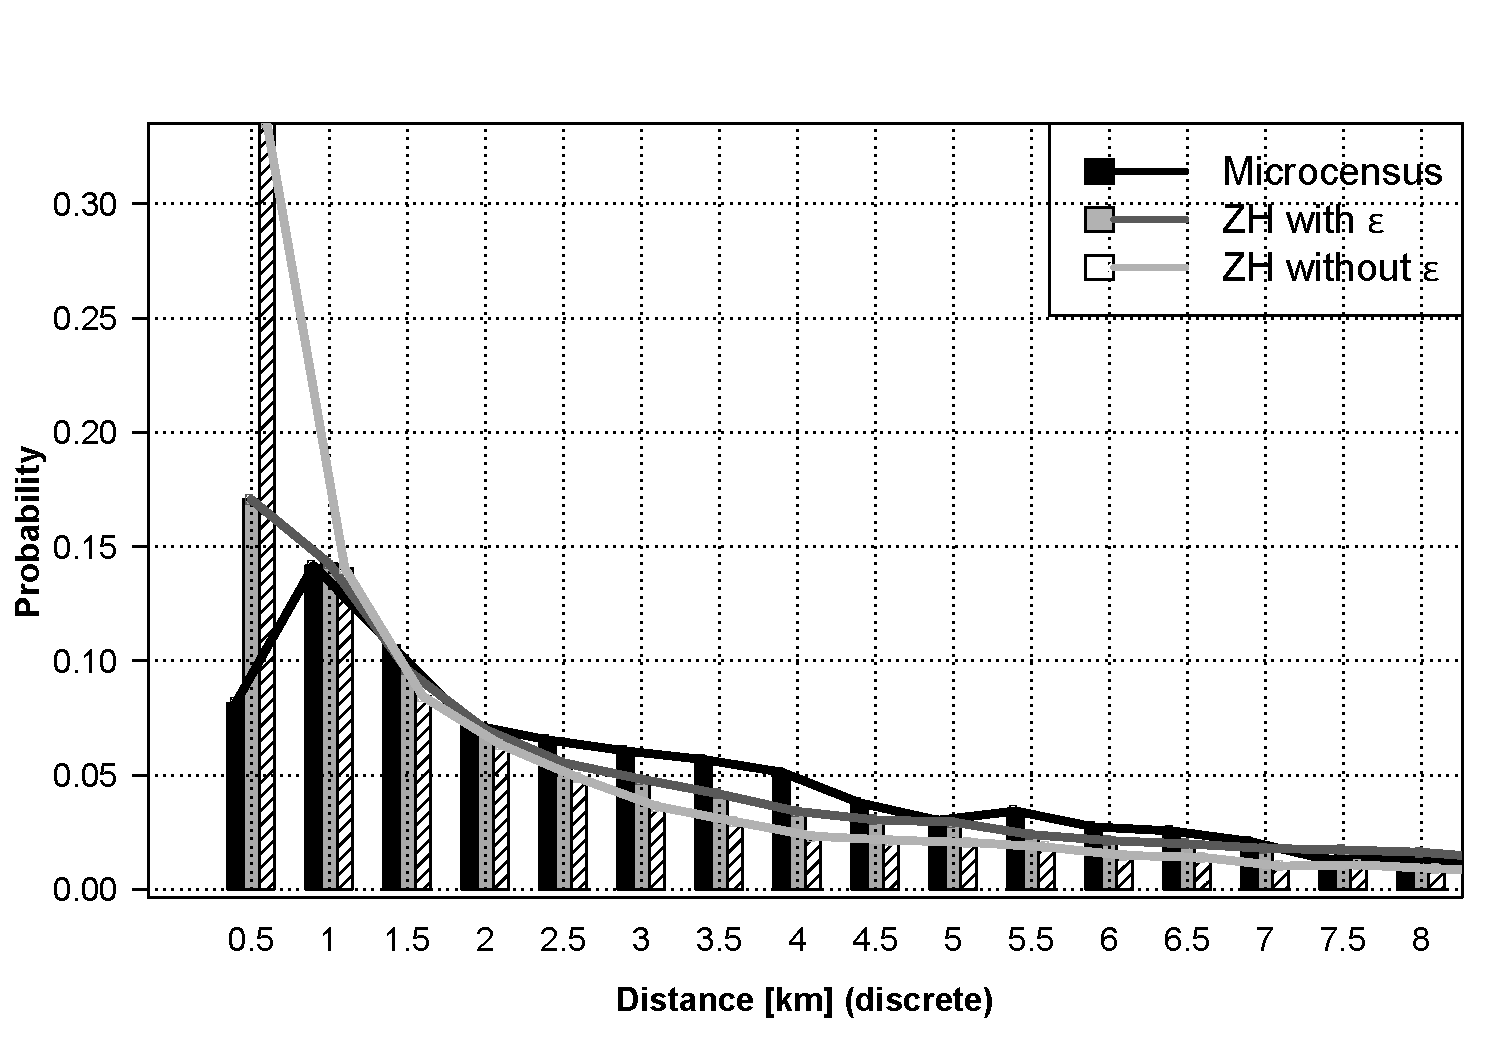
\includegraphics[width=0.99\textwidth,angle=0]{extending/figures/dc/zhShopping.pdf}}%
  {\label{fig:zhShopping}}%
  {}%
   \createsubfigure%
  {Leisure trips}%
  {\includegraphics[width=0.99\textwidth,angle=0]{extending/figures/dc//zhLeisure.pdf}}%
  {\label{fig:zhLeisure}}%
  {}%
}%
{}

\createfigure%
{Daily traffic volumes for 123 links compared to traffic counts}%
{Daily traffic volumes for 123 links compared to traffic counts. Per link $k$ the relative error is used, i.e, $(vol_{simulated,k}-vol_{counted,k}) / vol_{counted,k}$.}%
{\label{fig:countsLEGO}}%
{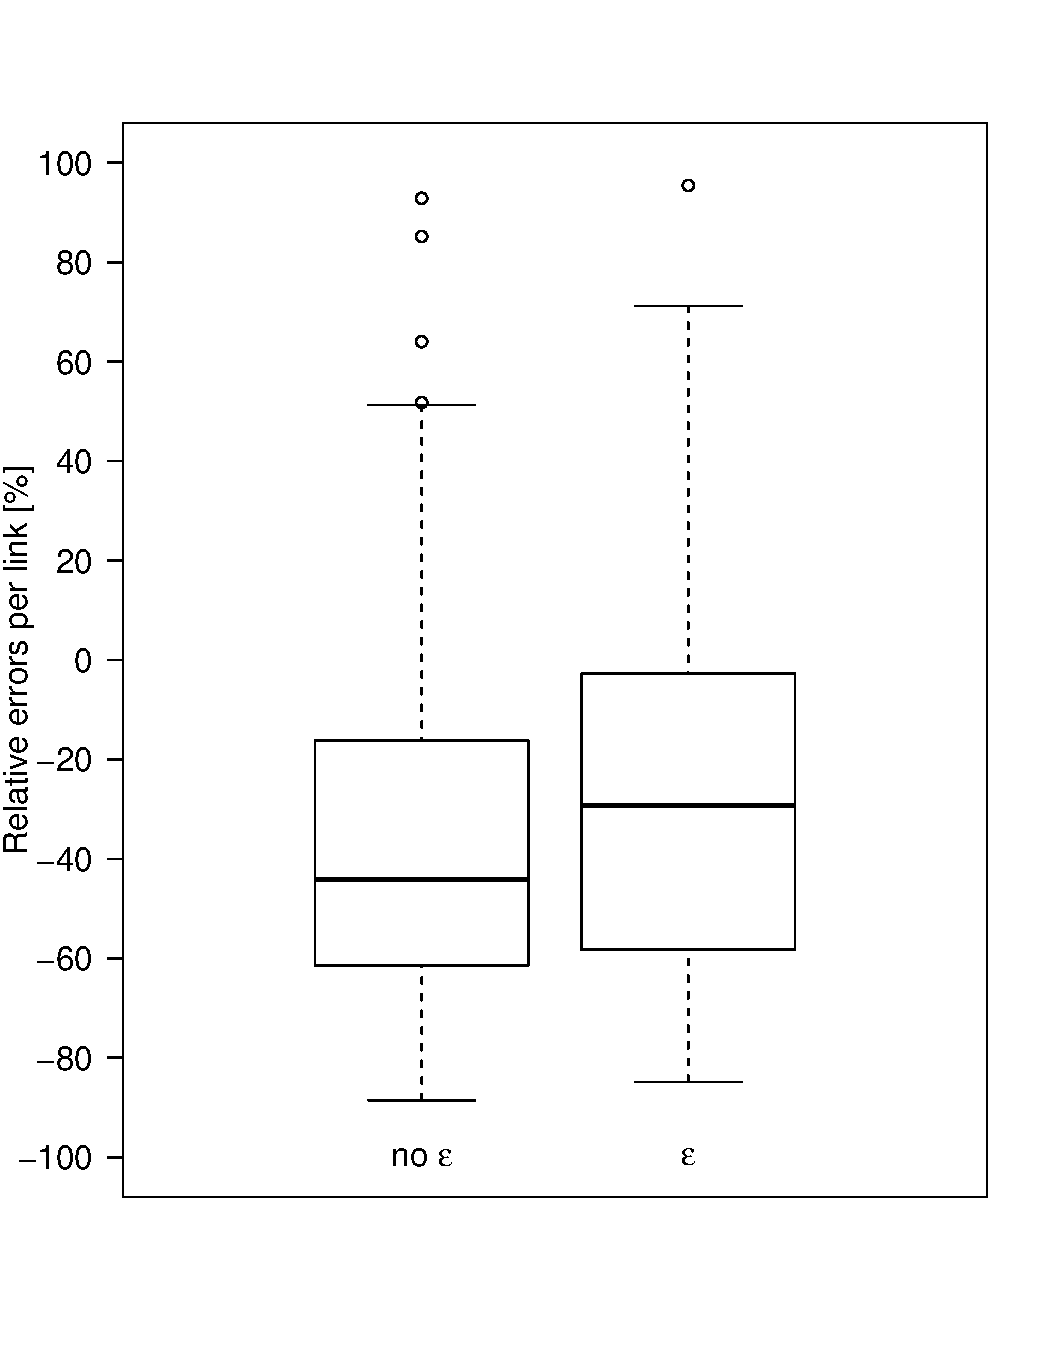
\includegraphics[width=0.8\textwidth, angle=0]{extending/figures/dc/zhCounts.pdf}}%
{}

% ##################################################################################################################
\section{Key Problems in Developing the Module}
Key problems of integrating destination choice into MATSim span behavioral and algorithmic issues. On the behavioral side, the specification of choice sets for model estimation is an unsolved problem to date. On the algorithmic side, as mentioned above, destination choice is in principle an ordinary optimization problem. However, as the agents interact and as the choices are embedded in a highly dynamic context, the problem becomes complex, even more as the targeted scenarios are usually large-scale. Thus, as is common for real-world optimization problems, solutions have to be based on problem-tailored heuristics \citep[][]{MichalewiczFogel_2004}. Important components of the MATSim destination choice are the construction of a limited search space and of the succeeding evaluation of this search space's elements. The main component however, is a mechanism to generate consistent random draws over the iterations necessary to include the objective function's error terms. This mechanisms is also applicable for other choice dimensions.

% --------------------------------------------------------------------
\subsection{Quenched Randomness}
In random utility theory, decision makers are assumed to be rational utility maximizers, where the utility is dependent on the characteristics of the alternatives, the choice maker itself and the choice situation. Besides these deterministic components, unobserved heterogeneity must be added by random error terms, often denoted $\varepsilon$. Due to these random error terms choices are quantified by probabilities dependent, for the logit model for example as $p_{n\ell q} = \exp(V_{n\ell q}) / \sum_L exp(V_{njq})$, where $V_{n\ell q}$ is person $n$'s systematic utility of alternative $\ell$ for activity $q$, which is divided by all remaining choice set's alternatives $j$. When drawing from the distribution specified by $p_{n\ell q}$ for a population, the aggregate choices are reproduced. This is basically also true, when applied in iterative frameworks. However, iterative frameworks are usually associated with some kind of learning or relaxation mechanism. This mechanism is heavily distorted by repeatedly and randomly drawing from $p_{n\ell q}$ in every iteration. In this case the $\varepsilon_{n\ell q}$ fluctuate from iteration to iteration, which is disastrous for the algorithm's convergence and behaviorally implausible.

Instead, the random error terms $\varepsilon$ need to remain fixed from iteration to iteration. The optimization is then performed as a deterministic search based on the resulting utilities $U_{n\ell q}$, i.e., an alternative $\ell$ for person $n$ and activity $q$ is selected as 
\[ 
\underset{\ell \in choice\: set}{\operatorname{argmax}} U_{nq} \,.
\] 
This includes, via the systematic part $V_{n\ell q}$, the disutility of traveling to destination~$\ell$ for activity~$q$.

As stated above, the random error terms need to remain the same over the iterations. In physics, this approach would be called ``quenched'' randomness; all randomness is computed initially and then attached to particles or destinations, rather than instantaneously generating it, which would be called ``annealed'' randomness. Two natural approaches for implementing quenched randomness are as follows:
\begin{itemize}
\item[(a)] Freezing the applied \emph{global} sequence of random numbers, meaning that a Monte Carlo method with the same random seed is used before and after the introduction of a policy measure and over the course of iterations. Thus, the error terms should come out the same way \emph{before} and \emph{after} the introduction of the policy measure. Differences in the outcome can thus be directly attributed to the policy measure. 
\item[(b)] Computing and storing a separate $\varepsilon_{n\ell q}$ for every combination of person $n$, alternative~$\ell$ and activity $q$.
\end{itemize}
 
Both strategies have flaws. Approach (a) is only an option if one is certain about every single aspect of the computational code. Importantly, one additional random number, drawn in one run but not in the other, completely destroys the ``quench'' for all decisions computed later in the program. Consistency is thus hard to achieve, especially in parallel or even distributed computing environments; according to personal communication a substantial machinery is necessary ensuring consistent choices. In a modular environment, as in MATSim, designed for external plugging-in of users' own modules---possibly drawing their own random numbers---the danger of destroying the quench is prohibitively high and thus approach (a) is impractical.

Approach (b) is certainly more robust. However, for large numbers of decision makers and/or alternatives, storing error terms is difficult. For destination choice, one quickly has $10^6$ decision makers and $10^6$ alternatives, resulting in $4 \times 10^{12} \hbox{Byte} = 4 \hbox{TByte}$ of storage space.

One may argue that this should not be a problem, since a normal person will rarely consider more than the order of a hundred alternatives in their choice set, reducing the computational problem. Aside from the necessity of storing every decision maker's choice set, this converts the computational problem into a conceptual one, since a good method to generate choice sets then needs to be found. With more conceptual progress, this may eventually be an option, but at this point, a conceptually simpler approach is preferred.

The developed solution below is generally applicable in econometric microsimulators. The same \emph{stable} error term can be \emph{re-}calculated on the fly by using stable random seeds $s_{n\ell q} = g(k_n, k_\ell, k_q)$, where are uniformly distributed random numbers associated with $k$, $\ell$, and $q$. That is, for each person $n$ a random number $k_n$ is generated and stored, and the same is done with each destination $\ell$. The value for the activity $q$ can be derived from its index in the plan possibly combined with the person's value $k_n$. This reduces the storage space dramatically from $\bar{nq} \times nn \times n\ell$ to $\bar{nq}(nn + n\ell)$, where $nn$ is the number of persons or agents and $n_\ell$ is the number of destinations and $\bar{nq}$ is the average number of discretionary activities in an agent's plan. This means that storage space is reduced to approx. $2 \times 4 \times 10^{6} \hbox{Byte} = 8 \hbox{MByte}$, which can be easily stored even on any modern machine.

The distribution of these seeds is essentially irrelevant; any error term distribution can be generated from any basic seed distribution. 
In the current version $g(k_n, k_\ell, k_q) = (k_n + k_\ell + k_q) \times v_{max}$ is used. $v_{max}$ is the maximum (long) number that can be handled by the specific machine.

To evaluate utility for a person $n$ visiting the destination $\ell$ for activity $q$ a sequence of Gumbel-distributed random numbers $seq_{n\ell q}$ is generated on the fly for every person-alternative-activity combination using the seed $s_{n\ell q}$. Some random number generators have problems in the initial phase of drawing, e.g., the first couple of random numbers are correlated or do never cover the complete probability space. As in our procedure the random number generator is constantly re-initialized, for these technical reasons, the error term $\varepsilon_{n\ell q}$ is derived not from the first element but from the $m^{th}$ element of the sequence $seq_{n\ell q}[m]$. Here, $m$ is set to 10. This procedure is valid as the set of all  $m^{th}$ elements of all different sequences is also a pseudo-random sequence following the same distribution as the sequences $seq_{n\ell q}$; clearly, \emph{true} random number generators relying on physical phenomena, such as hardware temperature, are not applicable. 

% ------------------------------------------
\subsection{Search Space Construction and Evaluation}
MATSim destination choice is based on best-response rather than random mutation, i.e., in every iteration the currently best alternative is chosen. This works as long as the inter-iteration changes are small, which is usually given by the relatively small share of agents who re-plan. The best-response approach is adopted due to the usually huge number of alternatives in combination with the search space characteristics. As the discrete search landscape is characterized by random noise because error terms are not (or only locally) spatially correlated (see Figure \ref{fig:landscape0}). For such problems---as opposed to continuous landscapes (see Figure \ref{fig:landscape1})---efficient search methods, such as local search methods, generally do not work.

% ---------------------------------
\createfigure%
{Search space}%
{Search space: The search algorithm is required to be able to handle correlated but also uncorrelated error terms as given by the MNL model. Local search methods, such as hill-climbing algorithms are only able to handle continuous search spaces, thus, for situation (a) a best-response global search algorithm is required.}%
{\label{fig:landscape}}%
{%
  \createsubfigure%
  {Uncorrelated error terms}%
  {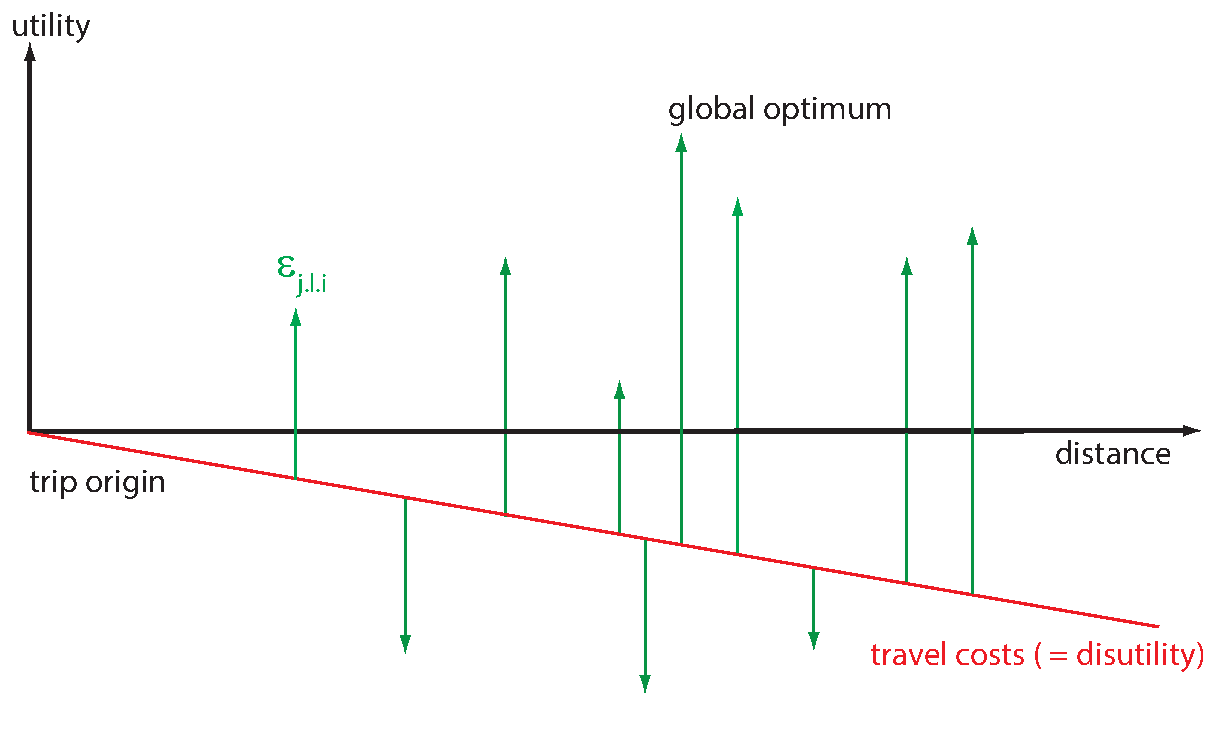
\includegraphics[width=0.8\textwidth,angle=0]{extending/figures/dc/landscape1.pdf}}%
  {\label{fig:landscape0}}%
  {}%
  \createsubfigure%
  {Spatially correlated error terms}%
	{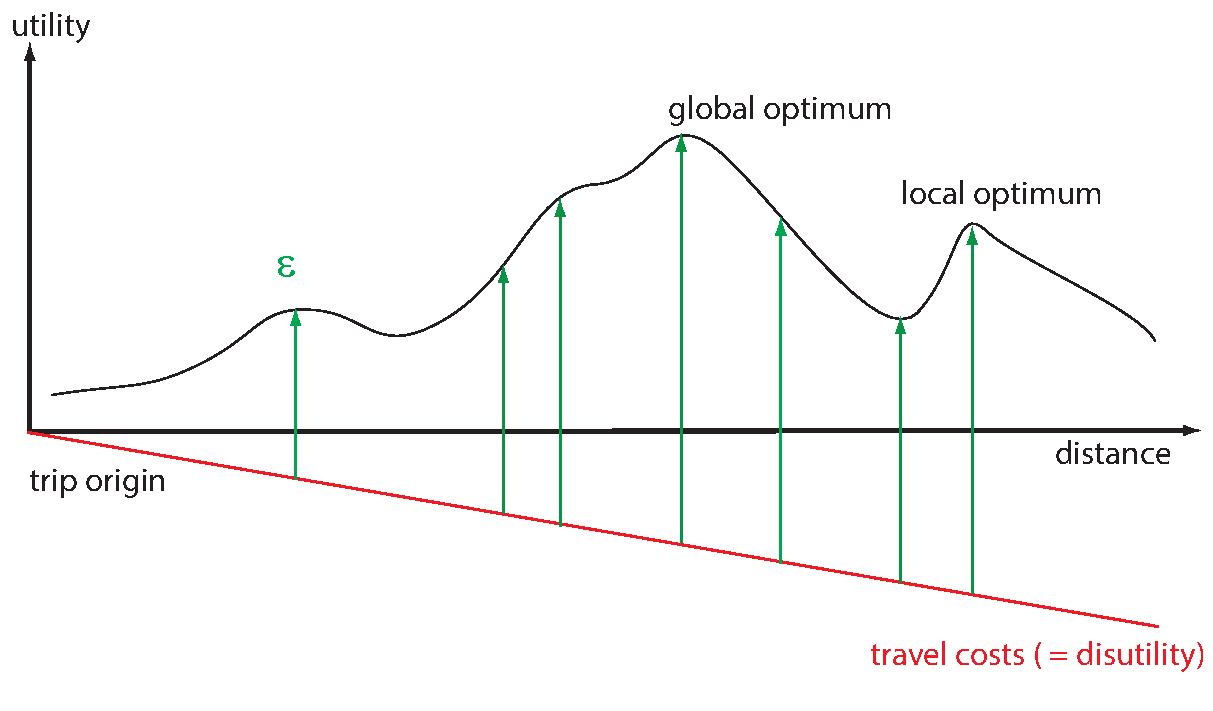
\includegraphics[width=0.8\textwidth,angle=0]{extending/figures/dc/landscape0.pdf}}%
  {\label{fig:landscape1}}%
  {}%
}%
{}

% ---------------------------------
On the search for the best choice, the large number of alternatives---prohibiting exhaustive search---is restrained as follows (for the detailed derivation see \citet[][p.51 ff.]{Horni_PhDThesis_2013}). It is assumed that travel costs are always negative, and that a person drops activities with negative net utility. Then the maximum potential travel effort a person is willing to invest is constrained by the maximum error term per person and activity. This approach is promising, as very large values for Gumbel-distributed are rare, meaning that a huge space must be searched for only a few persons. 

This reduction of the search space saves a lot of computation time, however, it is still infeasible and further speed-ups are necessary. Most computation time is due to calculation of travel times, i.e.,\ due to routing, for evaluation of the alternatives in the search space. To reduce these huge routing costs, the Dijkstra is not only applied forward---providing one-to-all travel times--but also \emph{backwards} using an average estimated arrival time as initial time. This is an approximation, and thus a \emph{probabilistic} best response is applied, justified by the natural assumption that, during the course of the iterations, the probabilistic choice probably reduces, or even compensates, the errors incurred by approximating travel times. 

With this procedure, the required computational effort is dramatically reduced, allowing application of destination choice to large-scale scenarios.

% ------------------------------------------
\subsection{Destination Choice Set Specification:}
While choice set specification is natural for choices with few alternatives, in contrast, for problems with a large universal choice set, usually present for spatial choices, such as destination or route choice, specifying individual choice sets becomes a challenging computational and even more behavioral issue (see e.g., \citet[][]{PagliaraTimmermans_TransLett_2009, Thill_PHG_1992, Schuessler_PhDThesis_2010, FrejingerEtAl_TransResB_2009}. Estimated parameters are sensitive to choice sets, and, at the same time, no established choice set definition procedure exists for spatial problems. This means that choice sets and, hence, estimation results are highly dependent on the modeler, which is an exogeneity problem, structurally similar to the well-known ``Modifiable Areal Unit Problem'' (MAUP), where results are dependent on modeler's zoning specification.

A prominent extension of the standard discrete choice modeling approach to treat this problem is formed by stochastic choice set models, founded by \citet[][]{Manski_TD_1977, BurnettKPHanson_TRR_1979, BurnettKP_UG_1980}, which integrates the choice set formation step into the estimation procedure by jointly estimating selection of a choice set and the choice of a particular alternative of this choice set \citep[][]{KaplanEtAl_TRB_2009, PagliaraTimmermans_TransLett_2009, Manski_TD_1977, Swait_TransResPartB_2001, HorowitzLouviere_IJRM_1995, BenAkivaBoccara_IJRM_1995, SwaitBenAkiva_TransResPartB_1987, Swait_TransResPartB_2001, MartinezEtAl_TransResPartB_2009, CascettaPapola_TransResPartA_2009, BierlaireEtAl_2_STRC_2009, ScroginEtAl_TechRep_UCF_2004, ManraiAndrews_EJOR_1998, Ansah_TransRes_1977}. Probabilistic choice set formation is conceptually appealing as choice sets are, in principle, not restrained a priori by exogenous criteria as in standard choice set specification. However, the procedure is in general associated with combinatorial complexity, making it computationally intractable. As a consequence, the practical approaches also require mechanisms to reduce the complexity of the choice set specification problem (see e.g., \citet[][p.11]{BenAkivaBoccara_IJRM_1995}). \citet[][]{ZhengJieGuo_TRB_2008}, for example, make the moderate assumption of continuous store choice sets (i.e., sets without ``holes'') around the trip origin, while the random-constraints model of \citet[][]{BenAkivaBoccara_IJRM_1995} exploits additional information on alternatives' availability for individuals.

Concluding, the destination choice set specification problem is still unsolved, meaning that the estimated models can only be fully consistently applied for the region, where the model was estimated. For MATSim, first destination choice model estimation efforts are reported in \citet[][Chapter 5]{Horni_PhDThesis_2013}.

% ##################################################################################################################
\section{The Module in the MATSim Context}
The destination choice module explicitly incorporates unobserved heterogeneity through random error terms. The standard MATSim utility function, however, does not contain error terms. The randomness measured in empirical data is included implicitly and in an uncontrolled way through the stochasticity of the simulation process. For destination choice, this has led to a dramatic underestimation of total travel demand making inclusion of unobserved heterogeneity inevitable. In the future, it should be researched if the standard utility function might also profit from the innovations of the destination choice module.

MATSim replanning offers different strategies to adapt plans ranging from random mutation to approximate suggestions, to best response answers. Destination choice is based on best response due to the sheer size of the alternatives set. 

As discussed in Chapter \ref{ch:scoring}, final goal is the implementation of an estimated utility function. At the moment, however, the standard MATSim scoring is still based on the Charypar-Nagel function and extended ad hoc by few attributes. This is also true for the destination choice module. Thus, calibration---instead of estimation---of the utility function is performed such that measured travel distances are matched. Calibration is performed by scaling the error terms. 

Although, the destination choice utility function is based on the discrete choice framework, some conceptual differences to the common application of discrete choice models exist. As shown above, there is no drawing from discrete choice models but maximization of an iteration stable utility function. In relation to that, the set of alternatives is not necessarily limited a priori and, thus, has the notion of a search space and not of a choice set.

% ##################################################################################################################
\section{Lessons Learned}
Two interesting lessons have been learning while developing the destination choice module. The first is a lesson of interdependence of preferences and space and,  thus, the necessity to evaluate them in combination. When looking at distance distributions (e.g., Figure \ref{fig:zhLEGO}) one might think that the functional form directly represents the preferences. This is not necessarily the case. In our simulations, it is the result of a \emph{linear} travel disutility applied in geographic space, where the number of opportunities increases with the square of the radius, in other words, with the travel distance. A similar emergent effect is present when scaling the random error terms. Although, both negative and positive error terms are enlarged and the average remains stable, the distribution gets more skewed toward the tail, as for the agents' choices the maximum values and not average values are relevant.

The second lesson concerns simulation results' variability. Although, random elements are not only present in destination choice, it was at the time of its development, the largest contributor of endogenous variability and made necessary the experiments presented in Section \ref{sec:variability}.

% ===============================================================================================
\section{Further Reading}
The main information source is \citet[][]{Horni_PhDThesis_2013}. Technical details and documentation are available at \citet[][]{MATSIM-T-DC_Webpage_2014}. Further reading related to destination choice is \citet[][]{HorniEtAl_IATBRspec_2013}, looking at parking, or \citet[][]{HorniEtAl_TechRep_IVT_2012}, coupling customers' and retailers' choices or in other words the supply and the demand side.

% ##################################################################################################################

% ======================================================================================================================
\paragraph{Facility Load:}
%The influence of interaction in \emph{transport} infrastructure for people's route and departure time choice has been recognized early \citep[e.\,g.,][]{Pigou_1920, Knight_QJE_1924, Wardrop_PICE_1952}. Similarly, it can be reasonably assumed that agent interaction in \emph{activities} infrastructure affects travel choices \citep[][]{Axhausen_SSRL_2006}. Marketing science provides ample evidence that agent interactions influence utility of performing an activity, where it can have both, positive or negative influence \citep[][p.331]{BakerJEtAl_JAMS_1994}, \citep[][]{ErogluAndHarrell_JR_1986, ErogluAndMachleit_JR_1990, ErogluEtAl_JBR_2005, HarrellEtAl_JMR_1980, HuiAndBateson_JCR_1991, PonsEtAl_PsychMark_2006}.
%
%In \citet[][]{HorniEtAl_TRR_2009}, based on the Zürich scenario, a singly-constrained model is presented that introduces competition for space-time slots on the activity infrastructure. The actual load is coupled with time-dependent capacity restraints for every activity location and incorporated explicitly into the agent's destination choice process as detailed below. 
%
%Activity location load, computed for time bins of 15 minutes, is derived from events that are delivered by the Mobsim. The load of one particular iteration combined with time-dependent activity location capacity restraints is considered in the agents' choice process of the succeeding iteration. In detail, this means that the utility function term $S_{dur,q}$, described above, is multiplied by $max(0; 1 - f_{load\ penalty})$ penalizing the agents dependent on the load of the location they frequented. $f_{load\ penalty}$ is a power function, as this has shown to be a good choice for modeling capacity restraints (remember that the well-known cost-flow function by \citet[][]{TA_manual_1964} is a power function). To introduce additional heterogeneity regarding the activity locations, an attractiveness factor $f_{attractiveness}$ is introduced that is defined to be logarithmically dependent on the store size given by the official census of workplaces.
%
%Likewise for demonstration purposes, capacity restraints are exclusively applied to shopping locations, where in principle leisure activity locations could be handled similarly. However, deriving capacity restraints for leisure activity locations is expected to be much more difficult than for shopping locations because data availability is much smaller for leisure locations and capacity restraints vary much more between different leisure locations than between different shopping activities (hiking versus going to the movies might be an illustrative example).
%
%The model allows the assignment of individual time-dependent capacities to the activity locations. For the sake of demonstration, the capacities of all shopping facilities are set equal, where the values are derived from the shopping trip information given in the National Travel Survey of 2005. The total daily capacity is set so that the activity locations located in the region of Zurich satisfy the total daily demand with a reserve of 50\%. In detail, the capacity restraint function for a location $l$ is as follows:
%
%\[
%f_{load\ penalty, \ell}=\alpha_l \cdot \Bigg(\frac{load_{\ell}}{capacity_{\ell}}\Bigg)^{\beta_\ell}
%\]
%with $\alpha_\ell=1/1.5^{\beta_\ell}$, $\beta_\ell=5$. $f_{load\ penalty, \ell}$ is the penalty factor for location $\ell$ as described above.
%
%The simultaneous computation of the score reduction for all agents avoids the last-record problem discussed in \citet[][]{VovshaEtAl_TRR_2002}. Therein, a sequential choice process is proposed where alternatives are removed from the choice set of the later travelers if the locations are already occupied by the earlier travelers. Thereby, the order of the travelers is specified arbitrarily and thus the last-record problem (the last travelers have to travel far to find an available location) is not negligible when modeling heterogeneous travelers. 
%
%As expected, the constrained model improves results' quality by reducing the number of implausibly overcrowded activity locations.

% ======================================================================================================================
\paragraph{Error Terms:}
%MATSim as a utility-maximizing model is strongly related to the discrete choice framework, meaning that this framework might guide the MATSim utility function specification. Utility in discrete choice models is composed of a deterministic part and a random error term. The random error term represents the unobserved heterogeneity, i.e., it subsumes, both, truly, i.e., inherently random decisions and the modeler's missing knowledge about the choice and its context. 
%
%In MATSim, the utility function for route, mode and time choice does not contain a random error term (yet). This can be regarded as a shortcoming of the model. However, this is at least partially compensated through the stochasticity of the replanning. First, route and time choices are usually subject to significant competition. The co-evolutionary algorithm of MATSim, detailed below, essentially assigns the resources in a random manner to the persons. For example, two identical persons may end up with different routes according to the order in which they undergo the replanning. Essentially, this means that a random term is present in the choice modeling. However, this randomness is introduced implicitly and not in a systematic manner. In other words, choice outcomes do not only depend on implemented choice model, but are also implicitly influenced by the implementation of the algorithm to find the solutions of the utility-maximization. This is difficult to interpret, and, furthermore, replanning did up to now not add enough unobserved heterogeneity to destination choice. Thus, an explicit random error term $\varepsilon_{n\ell q}$ for every person $n$, alternative $\ell$ and activity $q$, held stable over the iterations, is added to the destination choice utility function \citep[][]{Horni_PhDThesis_2013}. Research about the necessity of error terms for the remaining choice dimensions is required.

 \cleardoublepage

\chapter{Within-Day Replanning}
\label{ch:withinday}
% ##################################################################################################################

\hfill \textbf{Authors:} Christoph Dobler, Kai Nagel

\begin{center} \includegraphics[width=0.6\textwidth, angle=0]{extending/figures/WithinDayReplanning/WithinDayMATSimLoop} \end{center}

\editdone{This text has undergone the professional edit. Please no grammatical changes anymore! They are most-probably wrong.}

% ##################################################################################################################
% NOTE: The standard information layout is non-standard, thus it uses the ``basic'' command.  kai, dec'14
\section{Basic Information}
\label{sec:withinDay-stdInfo}
% ============================================================================================
\subsection{Implementation Alternative 1:}
\label{sec:withinDay1-stdInfo}

\createStandardInformationBasic{%
%
\url{http://matsim.org/javadoc} $\to$ core $\to$ \lstinline{org.matsim.withinday} package
%
}{%
%
\url{http://matsim.org/javadoc} $\to$ core $\to$ \lstinline{RunWithinDayExample} class 
%
}{%
%
no configuration from config file possible
%
}{
%
See Section~\ref{sec:impl-plan-based}.
%
}

% ============================================================================================
\subsection{Implementation Alternative 2:}
\label{sec:withinDay2-stdInfo}

\createStandardInformationBasic{%
%
\url{http://matsim.org/javadoc} $\to$ core $\to$ \lstinline{DriverAgent} class, \lstinline{MobsimAgent} class
%
}{%
%
\url{http://matsim.org/javadoc} $\to$ tutorial $\to$ \lstinline{RunOwnMobsimAgentUsingRouter} class
%
}{%
%
no configuration from config file possible
%
}{%
%
See Chapter~\ref{sec:dynAgent}.
%
}

% ##################################################################################################################
\section{Introduction}
In recent years, transport planning and traffic management interest in unforeseeable, or only partially foreseeable events within scenarios has increased. Partially foreseeable events often occur with taxis and car sharing. For example, agents with a planned taxi trip cannot know in advance which taxi will be available when they need one. When using car sharing, an agent might walk to the car sharing station and check whether a car is available or not. If it is not, the agent could either decide to wait, or change its plan and switch to another transportation mode. Road accidents, terrorist attacks or disasters such as earthquakes are examples of completely unpredictable events.

As discussed earlier, traditional simulation approaches (used in default-\gls{matsim}) calculate demand-supply equilibria using an iterative process. There, it is assumed that a typical situation is simulated where agents can rely on their experience from comparable situations, like previous iterations. Applying an iterative approach to a scenario with unexpected events results in problems like illogical agent behavior, producing false results. In the next section, these problems, as well as an alternative simulation approach, are presented. On one hand, this approach---called within-day replanning---simulates only a single iteration, avoiding problems resulting from an iterative simulation process. On the other hand, this approach does require a more detailed behavioral model for the agents. Subsequently, using \gls{matsim} as a base, the iterative approach is discussed, followed by two different implementations of the within-day replanning approach into the \gls{framework}, including discussions of the technical implementations.

% ##################################################################################################################
\section{Simulation Approaches} 
\label{sec:SimulationApproaches}
% ============================================================================================
\subsection{Iterative Simulation Approaches} 
\label{sec:IterativeSimulationApproaches}
%The starting point of an iterative simulation approach, as it is used in agent-based traffic flow micro-simulations like DYNEMO \citep{Schwerdtfeger_VolmulerHamerslag_1984, NoekelSchmidt_NSE_2002}, MATSim \citep{Balmer_PhDThesis_2007, BalmerEtAl_HEUREKA_2008} or TRANSIMS \citep{SmithEtAl_NTRPAC_1995, NagelRickert_ParComp_2001},  is the generation of an initial plan for each agent (e.g.,\,based on census and~/~or travel diary data). A plan contains an agent's intended schedule of activities and the trips that connect them. For each activity, its type (e.g.,\,\emph{work}, \emph{leisure} or \emph{shopping}), its location and the expected start and end time are given. A transport mode and a route specify a trip. The iterative optimization process consists of three steps. First, a mobility simulation executes the plans which are then evaluated using a fitness function. Finally, agents must select plans to be executed in the next iteration. Each agent can keep several plans in its memory. Bad plans can be deleted and new plans created by cloning and adapting existing ones using information (e.g.,\,travel times) from one or more previous iterations. The allowed adaption operations define the optimization search space (e.g.,\,routes, location and start / end times of activities). This iterative optimization can be seen as a period-to-period replanning strategy. Since one day is a commonly used duration, it is often called day-to-day replanning strategy.

An iterative day-to-day replanning approach is appropriate as long as the scenario describes a \emph{typical} situation or day. For such scenarios, it is feasible to assume that agents are familiar with typically occurring events like traffic jams during peak hours. Therefore, they try to avoid driving during those times, or use alternative routes with less traffic. However, if the scenario contains unexpected events that the agents cannot foresee (e.g.,\,accidents or heavy weather conditions), using an iterative approach is not an appropriate choice. First, user equilibrium will not be reached in such a scenario because agents do not have enough information to choose optimal routes and daily activity plans. Another problem is the optimization process itself. Even if an agent chooses its routes randomly due to a lack of information, it will eventually find a good route if it tries enough different routes.

%---------------------------------------------------------------------
\createfigure%
{Exceptional event in a network}%
{Exceptional event in a network}%
{\label{fig:labelExceptionalEventExample}}%
{%
  \createsubfigure%
  {Network with planned route}%
  {\includegraphics[width=0.43\textwidth, angle=0]{extending/figures/WithinDayReplanning/network_original_route}}%
  {\label{fig:labelNetworkPlannedRoute}}%
  {\qquad}%
  \createsubfigure%
  {Network with exceptional event}%
  {\includegraphics[width=0.43\textwidth, angle=0]{extending/figures/WithinDayReplanning/network_exceptional_event}}%
  {\label{fig:labelNetworkExceptionalEvent}}%
  {\vspace{5mm}}%

  \createsubfigure%
  {Network with exceptional event and planned route}%
  {\includegraphics[width=0.43\textwidth, angle=0]{extending/figures/WithinDayReplanning/network_original_route_with_event}}%
  {\label{fig:labelNetworkExceptionalEventPlannedRoute}}%
  {\qquad}%
  \createsubfigure%
  {Network with exceptional event and adapted route}%
  {\includegraphics[width=0.43\textwidth, angle=0]{extending/figures/WithinDayReplanning/network_adapted_route_with_event}}%
  {\label{fig:labelNetworkExceptionalEventAdaptedRoute}}%
  {}%
}%
{}
%---------------------------------------------------------------------

Figure~\ref{fig:labelExceptionalEventExample} shows a simple example scenario where an iterative approach would produce illogical and faulty results. In Figure~\ref{fig:labelNetworkPlannedRoute}, an agent's planned route in a sample network is shown, including the times when the driver passes each node of the route. Clearly, those times are only valid if no exceptional event occurs. Figure~\ref{fig:labelNetworkExceptionalEvent} shows a link where an event, like an accident, blocks that link for two hours. As a result, the agent reaches its destination two hours later than expected (Figure~\ref{fig:labelNetworkExceptionalEventPlannedRoute}). When this scenario is iterated, the agent recognizes that its route has a much higher travel time than expected and therefore it will choose another route. The traffic jam caused by the accident will probably also increase travel times on links next to the blocked link. Therefore, the agent might find a route which is quite different than the original one (Figure~\ref{fig:labelNetworkExceptionalEventAdaptedRoute}). A closer look at the node where the new route deviates for the first time from the original one shows that this occurs even before the accident happened, which is unfeasible and illogical.

An obvious solution to avoiding such problems is using an alternative simulation approach without an iterative optimization process. The next section discusses such an approach and the requirements that must be fulfilled.

% ============================================================================================
\subsection{Within-Day Replanning Approach}
A within-day replanning approach uses a significantly different strategy from that of an iterative approach. Instead of multiple iterations, only a single one is simulated. Thus, it is now essential that agents can adapt their plans during this iteration without having information from previous iterations available. To do so, they have to continuously collect information and take into account their desires, beliefs and intentions when they decide how to (re)act.

While iterative approaches can use best-response modules, a within-day approach has to use something that might be called a best-guess module. Travel times are an obvious example. In an iterative approach, travel times can be collected from the previous iteration or even be averaged over several past iterations. The nearer a stable system is to a relaxed state, the smaller the differences in travel times between two iterations. This is not possible in a within-day approach. Even if an agent has perfect knowledge, it can only assume how the traffic flows will evolve in the future. To do so, it can take different information into account to estimate travel times. It could, for example, take travel times from a typical day without exceptional events and combine them with information it gathers during the simulated day. Depending on the amount and the quality of this information, the agent might rely more or less on its experience.

Therefore, the decision-making process of an agent becomes an important topic. In an iterative approach, each agent has total information and can thus select the best route. Due to limited available information, this is not possible in a within-day approach. One agent could, for example, choose a route where expected travel time is very short, but also very uncertain. Another agent might not be willing to take that risk and therefore select a longer route where the assumed travel time is more reliable. Perception of information might also vary between agents; one could rely on media traffic information, another might ignore it.

Each within-day replanning action is categorized by two parameters---the replanned element of the plan (an activity or a trip) and the point in time when the replanned plan element is executed (right now or at a future point in time). If an activity is replanned, several changes are possible. Its start and end time can be adapted, its location can be changed, it can be dropped, or created new from scratch. For a trip, origin and destination, route, mode of transport and departure time can be replanned. Often replanning one single plan element results in a chain reaction that forces replanning of other plan elements. If, for example, an activity is dropped, the trips from and to this activity have to be merged.

The second parameter categorizing a replanning action depends on when the replanned plan element is executed. This could be either the currently performed plan element or one being performed in the future. Clearly, in a currently performed plan element, not all previously mentioned replanning actions could be conducted. E.g.,\,start time of an activity or transport mode of a trip currently being performed can no longer be adapted.

Due to the limited available information, a within-day replanning approach will, in contrast to an iterative approach, not converge to a user equilibrium. Decisions made during the simulated time period may seem to be optimal when they are made. However, evaluated retrospectively, an agent might realize that they were not.

Figure~\ref{fig:labelWithinDayMATSimLoop} shows how within-day replanning can be integrated into \gls{matsim}'s iterative optimization loop. An additional block builds another (inner) loop with the mobility simulation. Depending on the type of simulated scenario, the outer loop can be skipped.
%---------------------------------------------------------------------
\createfigure%
{(Iterative) within-day replanning MATSim loop}%
{(Iterative) within-day replanning MATSim loop}%
{\label{fig:labelWithinDayMATSimLoop}}%
{\includegraphics[width=12.5cm, angle=0]{extending/figures/WithinDayReplanning/WithinDayMATSimLoop}}%
{}%
%---------------------------------------------------------------------

% ============================================================================================
\subsection{Combined Approaches} 
\label{sec:CombinedApproaches}
An alternative to iterative, or within-day replanning only approaches, is to combine them. An obvious application is solving situations that cannot be planned exactly in advance, like parking or car sharing. An agent is, for example, able to plan a parking activity, but it cannot anticipate which parking spots will be available when the agent arrives. Thus, within-day replanning can be used when the agent starts its parking choice.

Other agents might want to share their cars, so an actual meeting must be confirmed. This can be ensured using within-day replanning. If the driver arrives too early, a \emph{waiting} activity is added to its plan; otherwise the agent being picked up will perform a \emph{waiting} activity until the car arrives.

% ##################################################################################################################
\section{Implementation}
% ============================================================================================
\subsection{General Thoughts}
Within-day or en-route replanning means that travelers replan during the day or while they are on their route. This means that the simulation needs to find some way to influence the agent while the \gls{mobsim} (network loading) is running. For the \gls{matsim} main network loading module, the so-called \gls{qsim}, this could be achieved by inserting an agent-loop, as follows:
\begin{lstlisting}
   void doSimStep() {
      for ( each agent ) {   // <-- agent loop
         agent.doSimStep() ;
      }
      for ( each link ) {
         link.doSimStep() ;
      }
      for ( each node ) {
         node.doSimStep() ;
      }
   }  
\end{lstlisting}
In this loop, each agent has the chance to deliberate in every time step. Clearly, the agent can decide that he/she has nothing to deliberate and return immediately.

Such an approach does, however, lead to computational challenges. Going through all links and nodes in every time step is already an expensive operation and a number of efficiency improvements (such as "switching off non-active links") are contained in the code.  Also, the number of links or nodes is typically an order of magnitude smaller than the number of synthetic persons in a scenario. Thus, some massive optimization would have to be undertaken in order to make the above approach computationally efficient.

An alternative approach to the above is to ask each agent only when a decision needs to be made. The most important decision for a driver is to chose the next link, i.e.,\,\begin{lstlisting}
class MyDriverAgent implements DriverAgent {
   ...
   @Override
   public Id<Link> chooseNextLink() {
      <algorithm to determine ID of next link>
      return nextLinkId ;
   }
}
\end{lstlisting}
%
Similar implementations are needed for all other queries that could be asked of the agent, for example:
\begin{compactitem}
\item Should the trip end on the current link?
\item Should the agent get off at the current stop?
\item What is the \lstinline|ID| of the vehicle to be used for a trip?
\end{compactitem}
%
From the agent's perspective, such an approach might be called \emph{event driven}, since the agent performs only mental activity at such events.

There is, indeed, a mechanism to program such agents and to insert
them into the \gls{qsim}. This is discussed in more detail in Section~\ref{sec:impl-repl-the-ag}.

A challenge inherent in that approach is that the complete agent needs to be re-programmed.  This agent needs to have enough capabilities to be oriented about itself; for example, it needs to be able to compute plausible routes.

On the other hand, there are situations where the capability to decide the turn at each intersection while en-route is, in fact, not needed.  
%
For example, for typical evacuation applications, it makes sense to start all agents on their normal daily plans. When an emergency warning is distributed, the simulation can go once through all agents and decide how they react. This will be done by replacing some, or all, future elements of the current plan. In some applications, this may happen more than once; for example, if recommended evacuation directions change because of a shift in the wind. In other applications, evacuating agents could become stuck in unexpected congestion which might trigger en-route re-routing. This may, however, be restricted to relatively small regions, and it may be sufficient to go through such a replanning loop, perhaps every 300\,simulated seconds. 

For such applications, the plan-based approach (Section~\ref{sec:impl-plan-based}) is more suitable. Rather than having each agent answering certain queries in every time step or at every intersection, the plan-based approach first waits for a trigger (such as an emergency warning, or unexpected congestion), then decides on the affected agents,  then goes through those agents and changes the future part of their plans. This is not only conceptually easier than having every agent answer for him-/herself, but it is also computationally more efficient, since it is only called when it is triggered and impacts only the affected agents. 

Overall, implementers and users will have to balance their needs.  
%
If there are relatively few times when agents should re-plan, and these times can be easily identified by, i.e., corresponding to an emergency signal, then this is an indicator for the plan-based approach.  
%
If, on the other hand, an agent goes into the simulation mostly or entirely without a plan, like an entirely reactive taxi driver, then this speaks for replacing the agent.

\gls{matsim} provides infrastructure for both approaches. The plan-based approach currently provides more support infrastructure, i.e.,\,many important use cases can be implemented by re-using existing methods. The approach that replaces the agent, in contrast, provides more flexibility. In particular, it allows agents to make decisions at the latest possible time without additional computational overhead.  While this is not entirely realistic behaviorally, such an approach is often desirable from a simulation perspective, where one does not want reproducibility of simulations depend on, e.g.,\,random elements such as how far an agent plans ahead.

% ============================================================================================
\subsection{Implementation Alternative 1: Plan-Based Implementation}
\label{sec:impl-plan-based}
%\kai{Christoph, die ``mnote'' sind für mich, damit ich einen schnellen Überblick habe, was Du geschrieben hast.  Damit ich das nicht wiederhole, sondern mich ggf.\ darauf beziehe.}
%
%\mnote{day-to-day loop no longer necessary}

When adding within-day replanning to \gls{matsim}, its iterative loop (see Figure~\ref{fig:matsimcycle}) has to be adapted as shown in Figure~\ref{fig:labelWithinDayMATSimLoop}. On one hand, the additional \emph{within-day replanning} module is added, which interacts with the \gls{mobsim}. On the other hand, multiple iterations are only necessary if a combined simulation approach is used.
%
%\mnote{implementation as MobsimEngine ... tracking agents and plans}

The implementation is realized as so-called \lstinline{MobsimEngine} which can be plugged into the \gls{qsim}. In every simulated time step, the \gls{qsim} iterates over all registered \lstinline{MobsimEngines} and allows them to simulate the current time step. Besides simulation of the traffic flows, those engines are also able to let agents start or end activities. The engine containing the within-day replanning logic (called \lstinline{WithinDayEngine}) does not simulate traffic flows, but tracks agents and adapts their plans. Doing so is separated into two steps. First, agents whose plans have to be adapted in the current time step are identified. In a second step, the adaption of their plans is performed. 
%
%\mnote{register identifiers with replanners, replanners with the within-day engine}

Figure~\ref{fig:labelWithinDayEngine} shows the structure of the \lstinline{WithinDayEngine}. Multiple \lstinline{Replanners} can be registered to the engine. Each \lstinline{Replanner} represents a unique replanning strategy like re-routing or time mutation and uses a set of \lstinline{Identifiers} that communicate with agents and select those who are given the opportunity to adapt their plans. An \lstinline{Identifier} can be seen as an information-distributing unit, like a radio station or a policeman. Therefore, not every \emph{Identifier} communicates with all agents. For example, agents at home will probably listen to the radio, but agents walking in the park will not. Each \lstinline{Identifier} returns a list of agents to its superior \lstinline{Replanner}, which then adapts those agents' plans.

%---------------------------------------------------------------------
\createfigure%
{WithinDayEngine}%
{WithinDayEngine}%
{\label{fig:labelWithinDayEngine}}%
{\includegraphics[width=8.0cm, angle=0]{extending/figures/WithinDayReplanning/ReplanningManager}}%
{}
%---------------------------------------------------------------------
%
%\mnote{more about itentifiers and replanners}

Responsibilities are divided between \lstinline{Replanners} and \lstinline{Identifiers}. The first ones are responsible for adapting the agents' plans, but they should not check whether an agent should be replanned or not. If, for example, a \lstinline{Replanner} updates an agent's route, it has to be ensured by the \lstinline{Identifiers} that only agents who are currently performing a leg are replanned. In turn, \lstinline{Identifiers} should select agents who have to be replanned but should not change their plans. As a result of this division, the often time-consuming replanning of the agents' plans can be performed using parallel threads, which leads to an almost linear speed-up. In general, simulation results do not depend on the order in which agents are replanned. \emph{Replanners} which use random numbers are a special case. 
%They have to ensure that 
In the present implementation, their \emph{random number generator} is re-initialized for every replanned agent, using a deterministic value (e.g.,\,a combination of the agent's ID and the current time step). On one hand, this ensures that an agent's decisions can be reproduced even when the global sequence of random numbers changes. On the other hand, the simulation outcomes do not change if the number of threads used for the replanning is changed.
% \kai{Christoph, ist es das?  ``have to'' (wie Du es vorher hattest), erscheint mir auf jeden Fall zu stark.  Oder hat es etwas mit multi-threading zu tun?}
%
%\mnote{identifiers run sequentially}

Running the \lstinline{Identifier(s)} to select those agents who have to adapt their plans is performed sequentially. On one hand, an \lstinline{Identifier}'s runtime is typically very short and therefore no significant performance losses are expected. On the other hand, 
%it is a robust design which 
this makes the design robust so it cannot produce race conditions which could occur if multiple instances of an \lstinline{Identifier} run concurrently. An example would be an \lstinline{Identifier}, which selects agents on household level, i.e.,\,if a member of a household is identified, also all other members are added to the list of agents who have to be replanned. In an approach with parallel running instances of an \lstinline{Identifier}, an instance could identify member A of a household while concurrently another instance could identify member B of the same household. As a result, the household's members would be duplicated in the list of agents to be replanned---once added by each \lstinline{Identifier} instance.
%
%\mnote{different basic replanners for current/future trips/acts}

\lstinline{Replanner} implementations are available for any basic change of an agent's scheduled daily plan. All trips and activities can be adapted, although some replanning operations are not available when trip or activity has already been started. Possible adaptations are:
\begin{compactitem}
    \item Current trip (route, destination)
    \item Future trip (add, remove, mode, route, origin, destination)
    \item Current activity (end time)
    \item Future activity (add, remove, location, type, start and end time)
\end{compactitem}
%
For complex plan adaptations, those basic \lstinline{Replanners} can be combined. If, for example, an agent currently performing a trip changes the destination of its next activity, routes of the current and next trip must be adapted.
%
%\mnote{different basic identifiers}

Additionally, four basic \lstinline{Identifiers} have been implemented so far. They identify agents, which are...
\begin{compactitem}
    \item Performing an activity.
    \item Performing an activity which will end in the current time step.
    \item Performing a trip.
    \item Performing a trip and are going to move to another link.
\end{compactitem}
%
%\mnote{AgentFilters (e.g.,\,for spatial areas)}

Often, identifiers have to handle only a subset of the population, e.g.,\,only male agents, or agents currently traveling in a car. To prevent that the same functionality having to be implemented multiple times, so-called \lstinline{AgentFilters} are introduced. Their task is to remove agents not meeting the filter criteria from an agent set. Using \lstinline{AgentFilters} not only avoids duplicated code, but can also reduce computation effort: for example, two \lstinline{Identifiers} which should identify only agents currently traveling in a certain part of the network. Without \lstinline{AgentFilters}, each of them would have to track all traveling agents and their current positions. When this functionality is moved to an \lstinline{AgentFilter}, the two \lstinline{Identifiers} can share a single instance of that filter.
%
%\mnote{filters: simple and re-usable; identifiers: complex and include decision-making}

Basically, simple and re-usable functionality should be implemented as \lstinline{AgentFilters}, while more complex and/or decision-making functionality should be part of an \lstinline{Identifier}. Again, an example: e.g.,\,a scenario modeling the search for a parking space: a filter can be utilized to take only agents currently traveling by car into account. The \lstinline{Identifier} solves the more complex tasks, such as deciding when the agent starts its search, or selecting the searching strategy to be applied.
%
%\mnote{basic AgentFilters}

Three basic \lstinline{AgentFilters} have been implemented so far. They filter agents which are not...
\begin{compactitem}
    \item Part of a predefined agent set.
    \item Currently using a transport mode included in a given set.
    \item Currently located on a link included in a predefined set.
\end{compactitem}
%
%\mnote{observers}

In addition to the logic identifying agents and adapting their plans, another important within-day replanning framework component is code that continuously collects information and provides it to the \lstinline{Identifiers}. These decide,based on that data, whether agents are replanned or not. In a time step-based approach---as realized by the \gls{qsim}---collecting, analyzing and aggregating data, as well as providing it, can be easily realized. Figure~\ref{fig:labelQSimTimeStep} shows the structure of a \gls{qsim}'s time step. Each time step is separated into three phases---\lstinline{before time step}, \lstinline{do sim step} and \lstinline{after time step}. During the \lstinline{do sim step} phase, all registered \lstinline{MobsimEngines} simulate the current time step. The \lstinline{before time step} and \lstinline{after time step} phases allow code execution before or after simulation of the current time step. A class can collect data such as link travel times during the \lstinline{do sim step} phase. Then, the collected data can be analyzed and aggregated in the \lstinline{after time step} phase. In the next time step, the \lstinline{WithinDayEngine's Identifiers} can use that data for their decisions. The \lstinline{WithinDayEngine} is always the first \lstinline{MobsimEngine} executing its \lstinline{doSimStep} method, ensuring that no agent has changed its status since the \lstinline{after time step} phase of the previous time step. As a result, the \lstinline{Identifiers} make their decisions on %actual 
current data.

%---------------------------------------------------------------------
\createfigure%
{\protect\gls{qsim} time step}%
{\protect\gls{qsim} time step}%
{\label{fig:labelQSimTimeStep}}%
{\includegraphics[width=8.0cm, angle=0]{extending/figures/WithinDayReplanning/QSimTimeStep}}%
{}
%---------------------------------------------------------------------
%
%\mnote{example: TravelTimeCollector}

An example of this type of class is the so-called \lstinline{TravelTimeCollector}. It provides actual link travel times to the \lstinline{Replanners} by collecting and averaging travel times of agents that have recently passed a link during a given time. A typical time span is 15\,minutes; older link travel times are ignored. Specific time span duration has an important impact on travel times reported to the \lstinline{Replanners}. On one hand, significant changes in link travel times will be communicated very slowly, if the time span is too long. On the other hand, a too short duration will overrate outliers.

The \lstinline{TravelTimeCollector} is a simple, but efficient, implementation of a within-day travel time calculator. It does not incorporate features like traffic flow predictions or dynamic recent travel times weighting based on historic data. 
%Due to 
Because it does not factor in such features, it is very robust, even in scenarios where traffic flow conditions change dramatically.

%---------------------------------------------------------------------
\createfigure%
{TravelTimeCollector}%
{TravelTimeCollector}%
{\label{fig:labelTravelTimeCollector}}%
{\includegraphics[width=8.0cm, angle=0]{extending/figures/WithinDayReplanning/TravelTimeCollector}}%
{}
%---------------------------------------------------------------------
%
%\mnote{matsim person vs.\ matsim agent}

The current \gls{matsim} code differentiates between \lstinline$Person$ and \lstinline$MobsimAgent$.  
%
\lstinline$Person$ can be seen as a very simple Q-learning entity, possessing multiple \lstinline$Plan$s ("actions"), each with an expected score updated with every plan run. Thus, a \lstinline$Person$ is consistent over the iterations; in fact, the internal state of each \lstinline$Person$ is written to file at the end of the iterations.
%
\lstinline$MobsimAgent$, in contrast, is instantiated every time the \gls{qsim} is called, and does not exist beyond the \gls{qsim} running time. A \lstinline$MobsimAgent$ is essentially reactive, queried by the framework about decisions when approaching intersections, arrival points, or public transit stops. In the standard implementation, these queries are answered by the plan, but other implementations can be used and/or additional \lstinline$MobsimAgent$s can be added which do not correspond to \lstinline$Person$s.
%
%\mnote{Which plan to modify}

This leads to a question; should within-day adaptations to the \lstinline$Plan$ be passed through to the \lstinline$Person$? Let us call the actual trajectory through the system the "executed plan"'. This can be different from the original plan, i.e.,\,a different route, different departure times, different modes, etc. The original plan cannot just be replaced by the executed plan, since it is not clear that the executed plan, when used as input, will have itself as expected output. In consequence, it is not possible to treat the executed plan together with the just-obtained score as an action-value pair in the sense of Q-learning, since the score was obtained from the \emph{original} plan, not from the executed plan.

As a result, the code uses a copy of the original plan and modifies the copy. The score, however, is given to the original plan. The implementation is able to 
%% \kai{"is able to"? (existiert das derzeit als Option?}
%% %
%% \dobi{Christoph: sollte da sein, sofern der Code nicht inzwischen zerschossen wurde. Ich hatte das für den Initial Routes Creation Abschnitt in meiner Diss verwendet. Ich wollte da auch nochmal genauer drauf schauen, was die produzierten Ergebnisse eigentlich bedeuten - habe ich dann aber irgendwie nie mehr Zeit dafür gefunden.}
% 
\emph{also} memorize the executed plan and add it to the set of plans. This functionality, however, is experimental.

%% \mnote{lskdjf}

%% An important aspect to be considered when using within-day replanning is whether persons' or only agents' plans are replanned. In this context, a person is a global object which exists during an entire simulation run. An agent represents a person in the (traffic flow) micro-simulation part of an iteration. Moreover, a person has several plans in its memory, an agent only a single one. By default, an agent's plan is only a copy of the  represented person's plan. Only the score of the person's plan is updated by MATSim's scoring module. 
%
%\mnote{parking example: parking search route should not be added to plan}

In certain situations, setting the original to the executed plan clearly does not make sense; a parking search is one \citep[][]{WaraichEtAl_unpub_TRB_2013, Waraich_unpub_IATBR_2012}. %% \kai{citation?}
%% \dobi{Christoph: keine. Eventuell könntem an den Absatz auch weglassen? Der Standard ist ja mittlerweile, dass man den Plan der Person nicht verändert. Andererseits wäre dann der Absatz unten (mit den initial Routes) eher interessant, weil der eben ein Beispiel dafür gibt, wo die Standardeinstellung nicht sinnvoll ist.}.
%% \ah{\citet[][]{WaraichEtAl_TechRep_IVT_2013_2, WaraichEtAl_TechRep_IVT_2012}. Komme weder an den einen noch an den anderen dran und kann die Frage deshalb nicht selber beantworten.}
%% \ah{Rashid: Hall Andi,

%% Wir mussten das parking + withinday aus zeit/Performance gründen abbrechen (wir sind momentan an einer psim + withinday + parking variante daran). Es gibt zwei Paper dazu: siehe oben.
%% }
%
%In a first example, within-day replanning is used to simulate agents' parking search. 
A person's plan contains, as destination, the location where a free parking space is expected. However, if the agent realizes in the mobility simulation that there is no free space left, it starts looking for a free parking spot. As a result, the agent's route is extended. This extension has to be local in the agent's route, since it is only necessary in the current iteration
and probably not in another one, where the initially selected parking spot is available.

%% \mnote{starting agents without routes: within-day routes \emph{should} be added to plan (but I don't agree)}

%Creating agents' initial routes using within-day replanning illustrates an application where persons' plans must be adapted. By default, creation of those routes is a step performed on a person level, before the micro-simulation is started. When this task is moved into the micro-simulation and is performed during their runtime, the created routes must still be stored in the person's plan. Otherwise they would be unavailable for later iterations. 
%\kai{Christoph, habe hier mal tentativ einen Absatz auskommentiert, der mir nicht wirklich hilfreich erscheint.  Solange der Plan, mit dem der Agent losfährt, derjenige ist, der den Score bekommt, ist es unerheblich, wann er berechnet wurde.}
%\kai{some pointers to simulations done with this set-up}

Capabilities of this within-day replanning implementation are shown and discussed by \citet{Dobler_PhDThesis_2013}, based on two sets of experiments. The first set is based on a model of Zürich city, where it is assumed that capacities of several city-center arterial roads are drastically reduced during the morning peak. Traveling agents are given the opportunity to bypass the resulting traffic jams by adapting their routes, using within-day replanning. As a result, average travel time of an agent affected by the incident is reduced from 42 to 23\,minutes. Also interesting is that even if only 50\,\% of the population adapts its routes, average travel times are reduced to 25\,minutes.
%\kai{Christoph: Vielleicht noch einen Satz über Ergebnisse (oder den vorhergehenden Satz umschreiben: Agents bypass the resulting traffic jams by adapting ..., leading to an overall readuction of travel times XX sec compared to the solution where agents stay on their original routes.} 

The second set of experiments uses within-day replanning to create agents' initial routes. The results are compared to runs where routes are created before the simulation starts, without traffic flow information. Results indicate that agents' average travel times are already very close to the values in a relaxed state. When using \gls{matsim}'s traditional approach, 10 to 15\,iterations must be performed before average travel times reach this level. %\kai{Christoph: Vielleicht noch einen Satz über Ergebnisse?}

% ============================================================================================
\subsection{Implementation Alternative~2: Replacing the Agent}
\label{sec:impl-repl-the-ag}
%% \kai{go through following and make consistent!!!}
According to \cite{RussellNorvigBook}, an agent is "anything that can be viewed as perceiving its environment through sensors and acting upon that environment through effectors."  As stated above, \gls{matsim} has agents on two levels:
%
\begin{compactitem}
	\item \lstinline$Person$ is a Q-learning agent that is persistent over the iterations.
	\item \lstinline$MobsimAgent$ is a reactive agent that only exists during the \gls{mobsim}.
\end{compactitem}

For the Q-learning agent, perception works through the events; i.e.,\,events are used to compute the score, build mental models to generate alternatives, etc. Acting on the environment works through plan selection.

For the reactive agent, perception works more directly through callback methods, such as the simulation notifying the agent it has just moved through an intersection. Acting on the environment works through making decisions at decision points, e.g.,\,about turning directions at intersections, or whether to board a certain bus.

As discussed, the approach described in Section~\ref{sec:impl-plan-based} assumes that the reactive agent still has followed (and generally follows) a plan. There may, however, be situations where this is inappropriate: for example, when the agent makes up the route as it goes, or when one wants to investigate models where each agent has its own perception and deliberation, rather than some external algorithm modifying its plan. As also mentioned earlier, there is no clear rule governing when and where an approach is better; it depends both on both project requirements and on the developer's personal preferences.
%
Here, with this in mind, we will look at \lstinline$MobsimAgent$s, which no longer have a pre-computed plan, but make decisions as they go. There is also a class of \lstinline$DynAgent$, which wrap around \lstinline$MobsimAgent$, making it easier to use and providing additional infrastructure (Section~\ref{sec:dynAgent}).

% ----------------------------------------------------------------------------
\subsubsection{Agent Interface}
The \lstinline$DriverAgent$ interface structurally resembles:
\begin{compactitem}
\item \lstinline$Id chooseNextLinkId()$---agent is asked at intersections and needs to return how to proceed.
%% \item \lstinline$Id<Link> getDestinationLinkId()$ -- agent is essentially asked if it wants to arrive on the current link.\footnote{%
%% The method can return {\tt null}.  Arguably, it should be modified to something like {\tt boolean isArrivingOnCurrentLink()}.
%% }  
\item \lstinline$boolean isWantingToArriveOnCurrentLink()$---agent is asked if it wants to arrive on the current link.
\item \lstinline$void notifyMoveOverNode(Id newLinkId)$---agent is notified that it has traversed the intersection and entered a new link.
\end{compactitem}
%
The rest comprises relatively simple bookkeeping methods like \lstinline$getId()$---the agent needs to know its own identifier.

If it is assumed that the agent does not only replan en-route, but also while at activities, then the \lstinline$MobsimAgent$ interface also must be implemented.  This is a bit more involved; important methods are:
\begin{compactitem}
\item \lstinline$endLegAndComputeNextState(...)$---agent is notified that the current transport leg has ended, and the agent internally needs to decide how to continue.
\item \lstinline$endActivityAndComputeNextState(...)$---agent is notified that current activity has ended; the agent internally needs to decide how to continue.
\item \lstinline$setStateToAbort(...)$---if a leg or an activity was not ended cleanly: this could happen if \lstinline$chooseNextLinkId()$ returns a link that is not outgoing from the current node.\footnote{%
%
Despite the name of the method, the agent can recover.  %
}
\item \lstinline$getState()$---agent needs to return its current state, which essentially either returns \lstinline$ACTIVITY$ or \lstinline|LEG|; most important here  is that the framework obtains information about whether the agent wants to start a new activity or leg.
\end{compactitem}
Again, everything else concerns bookkeeping methods.

% ----------------------------------------------------------------------
\subsubsection{Agent Insertion}
The code accepts several ways to insert such a self-programmed \lstinline$MobsimAgent$ into the code, but the preferred method is using the \lstinline$AgentSource$ interface, as follows:\footnote{%
%
See \url{http://matsim.org/javadoc} $\to$ core $\to$ the \lstinline{AgentSource} class for a pointer to a working code example.
%
}
\begin{lstlisting}[basicstyle=\footnotesize\tt]{}
class MyAgentSource implements AgentSource {
   // constructor
   MyAgentSource ( Guidance guidance ) {
      ...
   }
   public void insertAgentsIntoMobsim() {
      // insert agent:
      MobsimAgent ag = new MyMobsimAgent( guidance ) ;
      qsim.insertAgentIntoMobsim(ag) ;
        
      // insert vehicle:
      // ...
      qsim.createAndParkVehicleOnLink(veh, linkId );
   }
}
\end{lstlisting}
\lstinline$Guidance$ helps the agent with making decisions, see below.

% --------------------------------------------------------------------
\subsubsection{Perception, Decision, Integration}
The agents somehow need to perceive their environment. The simulation tells the agent where it is, via \lstinline|notifyMoveOverNode(Id<Link> nextLinkId)|. In general, however, this will not be sufficient. For example, the agent may want to be informed about congestion, or evacuation directions.

A general way to achieve this is to use the \lstinline$Events$ channel.

We would probably suggest separating observer, guidance, and the agent itself.

\paragraph{Observer}

The observer would probably listen to events:
\begin{lstlisting}
class MyObserver implements BasicEventHandler {
   @Override
   public void handleEvent(Event event) {
      ... // memorize information
   }
   ...
}
\end{lstlisting}
For working code, see \url{http://matsim.org/javadoc} $\to$ core $\to$ \lstinline{RunOwnMobsimAgentWithPerception} class and related.

\paragraph{Guidance}

A guidance object might give advice to agents, which could also be defined as a decision-making entity. This could, in principle, also be fully incorporated into the agent. It could, for example, be designed as follows:
\begin{lstlisting}
class MyGuidance {
   MyGuidance( MyObserver observer ) {
      ...
   }
   Id<Link> chooseNextLinkId( Id<Link> currentLinkId ) {
      ... // compute and return decision
   }
}
\end{lstlisting}
For working code, see \url{http://matsim.org/javadoc} $\to$ core $\to$ \lstinline{RunOwnMobsimAgentWithPerception} class and related.

\paragraph{Agent}

The agent needs access to guidance:
\begin{lstlisting}
class MyAgent implements MobsimDriverAgent {
   MyGuidance guidance ;
   MyAgent( MyGuidance guidance ) {
      this.guidance = guidance ;
   }  
   ...
   @Override
   Id<Link> chooseNextLinkId() {
      return this.guidance.chooseNextLinkId( this.currentLinkId ) ;
   }
   ...
}
\end{lstlisting}
For working code, see \url{http://matsim.org/javadoc} $\to$ core $\to$ \lstinline{RunOwnMobsimAgentWithPerception} class and related.

\paragraph{Control script}

This would be plugged together by a variant of the following script:
\begin{lstlisting}[basicstyle=\footnotesize\tt]{}
Controler ctrl = ... ;
...
// create observer object:
MyObserver observer = new MyObserver() ;
// add into events channel:
ctrl.addEventsHandler(observer) ;
// create guidance object:
MyGuidance guidance = new MyGuidance( observer ) ;
// create mobsim factory and set into controler:
ctrl.setMobsimFactory(new MobsimFactory(){
   public Mobsim createMobsim(Scenario sc, EventsManager ev ) {
      MobsimFactory factory = new QSimFactory() ; 
      QSim qsim = (QSim) factory.createMobsim(sc, ev) ;
      // add agent source into mobsim:
      qsim.addAgentSource( new MyAgentSource( guidance ) ) ;
      return qsim ;
   }
}) ;
...
ctrl.run() ;
\end{lstlisting}
The above "script" uses an anonymous class for the \lstinline$MobsimFactory$. This method of writing code is quite convenient for adapting \gls{matsim} to individual needs, also see Chapter~\ref{ch:extensionpoints}.

For working code, see \url{http://matsim.org/javadoc} $\to$ core $\to$ \lstinline{RunOwnMobsimAgentUsingRouter} class and related.

% ------------------------------------------------------------------
\subsubsection{Using Framework Methods}
\gls{matsim} uses a wide range of methods to plan the day of a simulated traveler. These can be passed into the guidance module, for example
\begin{lstlisting}
   Controler ctrl = new Controler(...) ;
   ...
   TripRouter router = ctrl.getTripRouterFactory().instantiateAndConfigureTripRouter() ;
   MyGuidance guidance = new MyGuidance( router ) ;
   ...
\end{lstlisting}
The guidance object can still be passed to the agent as it was before; it can now compute and then return, at each intersection, to make the best turn toward a destination.

%For working code, see \url{http://matsim.org/javadoc} $\to$ core $\to$ the \lstinline{RunOwnMobsimAgentWithPerception} class and related.
%\ah{Satz auskommentiert, da er ja schon in "Basic Information"' ganz oben (Section~\ref{sec:withinDay-stdInfo}) vorkommt. OK?}

% ---------------------------------------------------------------------
\subsubsection{\lstinline{DynAgent}}
As stated earlier, there is also a class \lstinline$DynAgent$. It wraps around  \lstinline$MobsimAgent$, making it easier to use and providing additional infrastructure (Section~\ref{sec:dynAgent}).
%% \mm{Kai, what do you mean by 'archaic'? In general, the architecture of DynAgent is much closer to the current version of PersonDriverAgentImpl.
%% DynAgentLogic produces next actions, like BasicPlanAgentImpl, and DynLegs (and DynActivities) are a kind of delegates for performing actions, like PlanBasedDriverAgentImpl is the delegate when it comes to driving.}

% ##################################################################################################################
% Local Variables:
% mode: latex
% mode: reftex
% mode: visual-line
% TeX-master: "../../main"
% comment-padding: 1
% fill-column: 9999
% End: 
 \cleardoublepage

\chapter{Public Transport}
\label{ch:pt}
% ##################################################################################################################

\hfill \textbf{Authors:} Marcel Rieser, Andreas Neumann, Johan W. Joubert, Sergio Arturo Ordóñez

\begin{center} \includegraphics[width=0.25\textwidth, angle=0]{extending/figures/ebr/Backwards.png} \end{center}

\editdone{This text has undergone the professional edit. Please no grammatical changes anymore! They are most-probably wrong.}

\section{Basic Information}

\subsection{Public Transit Extension}

\createStandardInformationBasic%
{\entryStd{core $\to$ \lstinline{org.matsim.pt} package}}%
{The module is invoked by enabling it in the configuration.}%
{\lstinline{transit} section(s) of the config file.}%
{\citet{Rieser2010}}

%%\ah{GTFS2TransitSchedule is also in there!} \kai{see below}

\subsection{Minibus Extension}

\createStandardInformationBasic%
{\entryStd{minibus}}%
{\invokeStd{minibus}{\lstinline{RunMinibus} class}}%
{\lstinline{transit} section(s) of the config file.}%
{\citet{Neumann2014PhD}}

\subsection{gtfs2matsimtransitschedule Extension}

%\createStandardInformationBasic%
%{\entryStd{minibus}}%
%{\invokeStd{minibus}{\lstinline{RunMinibus} class}}%
%{\lstinline{transit} section(s) of the config file.}%
%{-}

%%{\citet{Neumann2014PhD}}
%%\kai{Neimann2014 m.E.\ keine gute pub f gtfs2.... Oder?}
%%\kaitodo{check} 
%%\ah{m.E. war das sowieso falsch. gtfs2matsimtransitschedule (=Singapur) obwohl thematisch irgendwie verwandt hat nicht wirklich was mit Minibus zu tun, da gibt es ja gerade keine Schedule. Oder? Allerdings wird unten dann doch nicht die Schedule-Gen beschrieben.}

\createStandardInformationBasic%
{\entryStd{gtfs2matsimtransitschedule}}%
{\invokeStd{GTFS2TransitSchedule}{\lstinline{GTFS2MATSimTransitSchedule} class}}%
{no standard configuration.}%
{\citet{Ordonez_HKSTS_2011}}

\subsection{Events Based Public Transit Router}

\createStandardInformationBasic{
%
\entryStd{eventsBasedPTRouter}
%
}{%
%
\invokeStd{eventsBasedPTRouter}{\lstinline{RunControlerWS}, \lstinline{RunControlerWSV}, \lstinline{RunControlerWW} classes}%
%
}{}{%
%
\citet{OrdonezErath_TechRep_FCL_2013}%
%
}
% ##################################################################################################################
\section{Modeling Public Transport with MATSim}
\subsection{Introduction}
Public transport---or \emph{transit} as it is sometimes called---plays
an important role in many transport planning measures, even those initially
targeting only non-transit modes. By making other modes more or less
attractive (\eg by providing higher capacity with additional lanes, allowing
higher speeds, or charging money by setting up area road pricing), travelers
might reconsider their mode choice and switch to public transport (\emph{pt})
from other modes, or vice versa. Such changes can also occur when transit
infrastructure is changed; additional bus lines, changed tram routes with
different stops served, or altered headways---all are important for travelers
on specific lines, or public transport in general. Around~2007,
interest grew in extending \gls{matsim} to support detailed simulation of 
modes other than private car traffic, particularly public transport.

In a first step, \gls{matsim} was extended so that modes other than
\emph{car} would be \gls{teleported}; agents would be removed from one location
and placed at a later point of time---corresponding to estimated travel time---at
their destination location, where they could commence their next activity.
Together with a simple mode-choice module, randomly replacing all 
transport modes in all plan legs and a simple travel time estimation for
modes different than \emph{car}, first case studies resulting in modal share
changes were performed using \gls{matsim}
\citep{RieserGretherNagel2008modeChoiceCalculations,
GretherEtAl2009SimpleModeChoiceIPL}. This \gls{teleportation} mode is now available, by
default, in \gls{matsim} and still a very good fallback option to get a \gls{multimodal} scenario
up and running with as little data as possible.

In a second step, \gls{qsim} was extended to support detailed simulation of
public transport vehicles serving stops along fixed routes with a given schedule
\citep{Rieser2010}.
The next section describes, in more detail, data required and resulting features for this
detailed public transport simulation.

% ============================================================================================
\subsection{Data Model and Simulation Features}
\gls{matsim} supports very detailed modeling public transport; transit
vehicles run along the defined transit line routes, picking up
and dropping off passengers at stop locations, while monitoring transit
vehicles' capacities and maximum speeds. Data used to simulate public
transport in \gls{matsim} can be split in three parts:
%
\begin{itemize}\styleItemize
\item Stop locations
\item Schedule, defining lines, routes and departures
\item Vehicles
\end{itemize}

This data is stored in two files; vehicles are defined in one
file, stop locations and schedule in
another.
Examples of such files can be seen in
Section~\ref{sec:inputdata:transitvehicles} and
Section~\ref{sec:inputdata:transitschedule}, respectively.

The data model is comparable to other public transport planning
software, but simplified in several respects. A line typically has two or more
routes; one for each direction and additional routes when vehicles start
(or end) their service at some point on the full route (coming
from, or going to, a depot). Each transit route contains a network route,
specifying on which network links the transit vehicle drives, as well as
a list of departures, providing information about what time a vehicle
starts at the first route stop. A route also includes an ordered list
of stops served, along with timing information specifying when a vehicle
arrives or leaves a stop. This timing information is given as offsets only, to
be added to departure time at the first stop. Each departure contains the
time when a vehicle starts the route and a reference to the vehicle 
running this service. Because timing information is part of the route, routes
with the same stops sequence may exist, differing only in time offsets.
This is often the case with bus lines, that take traffic congestion and
longer rush hour waiting times at stops into account in the schedule. 

Stop locations are described by their coordinates and an optional name; they must
be assigned to exactly one line of the network for the simulation. Thus, they
can be best compared to ``stop points'' in \gls{visum}. There is, currently, no logical
grouping of stop locations to build a ``stop area''; this is a cluster of
stops often sharing the same name, but located on different intersection arms, 
served by different lines, many with transfer corridors for passengers.

Each vehicle belongs to one vehicle 'type', which describes various
characteristics, like seating and standing capacity (number of
passengers), its maximum speed and how many passengers can board or depart
a vehicle per second.

This data model already supports several advanced public transport modeling aspects: 
varying travel speeds along routes during different
times of day (important for improved simulation realism), using diverse vehicle types 
on routes at different times of day (interesting for schedule
economic analysis) and re-using transit vehicles for multiple
headways along one or different routes (allows vehicle deployment planning optimization, 
or research on delay-propagation effects).

With these data sets, the \gls{qsim} will simulate all transit vehicle movements.
The vehicles will start with their first route stop at the given
departure time, allow passengers to enter and then drive along their route,
serving stops. At each stop, passengers can enter or leave the vehicle.
The simulation generates additional, transit-related events whenever a transit
vehicle arrives or departs at a stop, when passengers enter or leave a vehicle,
but also when a passenger cannot board a vehicle because its capacity
limit is already reached. This allows for detailed analyses of \gls{matsim}'s public 
transport simulations.

For passengers to use public transport in \gls{matsim}, they must be able
to calculate a route using transit services. For this, \gls{matsim} includes a public
transport router that calculates the best route to the desired
destination with minimal cost, given a departure time. Costs are typically
defined only as travel time and a small penalty for changing lines, but other,
more complex cost functions could be used.

The routing algorithm is based on Dijkstra's shortest path algorithm
\citep{Dijkstra_NM_1959}, but modified to take
multiple possible transit stops, around the start and end coordinates,
into account to find a route. Multiple start and end stops must be considered
to generate more realistic transit routes; otherwise, agents could
be forced to travel first in the wrong direction, or wait at an infrequently
served bus stop, instead of going a bit further to a busy subway stop location.
By modifying the shortest path algorithm to work with multiple start and end
locations, a considerable performance gain was achieved when compared to the basic (and somewhat naive)
implementation that calculated a route for each combination of start/end location
and then chose the best outcome.
%
%"\Karen{Please check the meaning of this last sentence;
%it was not clear whether the last phrase of the sentence referred to the implementation with
%modifications or the basic version.  Thanks!}"
%\ah{I added ``(and somewhat naive)'' as I think it is quite precise}

% -----------------------------------------------------------------------
\subsection{File formats}

\subsubsection{\lstinline|transitVehicles.xml|}
\label{sec:inputdata:transitvehicles}

%%\kai{convert to normal vehicles?}

%%\ah{copied from let's get started:}
%%\kai{vehicles.xml?  (without ``transit''?)} \kai{Andreas, fyi: I think we are leaning towards having separate containers vehicles.xml and transitVehicles.xml.  Not yet implemented.}

To simulate public transport in \gls{matsim}, two additional input files are necessary. One is \lstinline|transitVehicles.xml|, which describes vehicles serving the lines: big buses, small buses, trains or light rail vehicles and description of each vehicle's passenger transport capacity.

Public transport vehicle description can be split into two parts; first, vehicle types must be described, specifying how many passengers a vehicle can transport (Note that the term ``vehicle'' can refer to multiple vehicles in reality, \eg a train with several wagons should be specified as one long vehicle with many seats). Second, actual vehicles must be listed. Each vehicle has an identifier and is a previously specified vehicle type. The following shows an example of a such a file, describing one vehicle  and two vehicles of the same type. 

\begin{xml}
<?xml version="1.0" encoding="UTF-8"?> 
<vehicleDefinitions xmlns="http://www.matsim.org/files/dtd" 
       xmlns:xsi="http://www.w3.org/2001/XMLSchema-instance" 
       xsi:schemaLocation="http://www.matsim.org/files/dtd 
			  http://www.matsim.org/files/dtd/vehicleDefinitions_v1.0.xsd"> 
	<vehicleType id="1"> 
      <description>Small Train</description> 
      <capacity> 
         <seats persons="50"/> 
         <standingRoom persons="30"/> 
      </capacity> 
      <length meter="50.0"/> 
   </vehicleType> 
   <vehicle id="tr_1" type="1"/> 
   <vehicle id="tr_2" type="1"/> 
</vehicleDefinitions>
\end{xml}

% -----------------------------------------------------------------------
\subsubsection{\lstinline|transitSchedule.xml|}
\label{sec:inputdata:transitschedule}
The second, rather complex, file necessary to simulate public transport is \lstinline|transitSchedule.xml|, containing information about stop facilities (bus stops, train stations, or other stop locations) and transit services.

In the first part, stop facilities must be defined; each one is given a coordinate, an identifier and a reference to a network link. The stop can only be served by vehicles driving on that specified link. It is also possible to specify both a name for the stop and whether other vehicles are blocked when a transit vehicle halts at a stop. This last attribute is useful when modeling \eg different bus stops, where one has a bay, while at another, the bus must stop on the road.

After stop facilities, transit lines, their routes and schedules are described. This is a hierarchical data structure; each line can have one or more routes, each with a route profile, network route and list of departures. The following listing is an example of a basic, but complete transit schedule.
%
\begin{xml}
<?xml version="1.0" encoding="UTF-8"?> 
<!DOCTYPE transitSchedule SYSTEM "http://www.matsim.org/files/dtd/transitSchedule_v1.dtd"> 
<transitSchedule> 
   <transitStops> 
      <stopFacility id="1" x="990.0"  y="0.0"   name="Adorf" 
           linkRefId="1" isBlocking="false"/> 
      <stopFacility id="2" x="1100.0" y="980.0" name="Beweiler" 
           linkRefId="2" isBlocking="true"/> 
      <stopFacility id="3" x="0.0"    y="10.0"  name="Cestadt" 
           linkRefId="3" isBlocking="false"/> 
   </transitStops> 
   <transitLine id="Blue Line"> 
      <transitRoute id="1"> 
         <description>Just a comment.</description> 
         <transportMode>bus</transportMode> 
         <routeProfile> 
            <stop refId="1" departureOffset="00:00:00"/> 
            <stop refId="2" arrivalOffset="00:02:30" departureOffset="00:03:00" 
                                                     awaitDeparture="true"/> 
            <stop refId="3" arrivalOffset="00:05:00" awaitDeparture="true"/> 
         </routeProfile> 
         <route> 
            <link refId="1"/> 
            <link refId="2"/> 
            <link refId="3"/> 
         </route> 
         <departures> 
            <departure id="1" departureTime="07:00:00" vehicleRefId="12"/> 
            <departure id="2" departureTime="07:05:00" vehicleRefId="23"/> 
            <departure id="3" departureTime="07:10:00" vehicleRefId="34"/> 
         </departures> 
      </transitRoute> 
   </transitLine> 
</transitSchedule>
\end{xml}

Each transit line must have a unique ID and each transit route has an ID, which must be unique within that one line, allowing the same route ID to be used with different lines. The \lstinline|transportMode| describes network links where the line runs. (Actually, this is not yet in force, although it might be in the future. It would be possible to let a bus run on train links in the simulation.)

The \lstinline|routeProfile| describes the stops this route serves; the route itself describes the series of network links the transit vehicle's driver must navigate, often referred to as network route. Note that the complete route, \ie all links the vehicle traverses, must be listed in the route, not only those with stops. All specified stops should occur along this route in correct order. Time offsets given for each stop in the \lstinline|routeProfile| describe relative time offsets to an actual departure time. If a bus departs at 7\,am, and stop~2 has a \lstinline|departureOffset| 3\,minutes, this must be read that the bus is expected to depart at 7:03\,am from the specific stop. All stops in the route profile must have a departure offset defined, except the last one. All stops, except the first one, can, optionally, have an arrival offset defined. This is useful for large trains that stop for several minutes at a station; helping the routing algorithm find connecting services at the correct time, namely the expected train arrival time.

As the last part of a transit route description, a departures list should be given. Each departure has an ID, which must be unique within the route, giving the departure time at the first stop of the specified route profile. The departure also specifies the vehicle (which must be defined in the previous transit vehicle list) with which the service should be run. 

Because of its complexity, transit schedules often contain small mistakes that will return in an error when the simulation runs. Typical examples include: missing links in the network route, or incorrect defined stop order on the network route. To ensure a schedule avoids such issues before the simulation starts, a special validation routine is available:
%
\begin{lstlisting}
java -Xmx512m -cp /path/to/matsim.jar  
      org.matsim.pt.utils.TransitScheduleValidator  
      /path/to/transitSchedule.xml /path/to/network.xml
\end{lstlisting}
%
If run, this validator will print out a list of errors or warnings, if any are found, or show a message that the schedule appears to be valid.

% ============================================================================================
\subsection{Possible Improvements}
While the ability to simulate public transport was a big advance for \gls{matsim},
several shortcomings still require attention:
%
\begin{itemize}\styleItemize
	\item The data model (and thus, the simulation) does not yet fully support some
	real world transit lines: for example, circular lines with no
	defined start and end cannot yet be easily modeled. Some bus or
	train lines also have stops where only boarding or alighting the vehicle is allowed,
	but not both (\eg overnight trains with sleeper cabins). At the moment, \gls{matsim}
	always allows boarding and alighting at stops, leading to agents \eg using a
	train with sleeper cabins for a short trip; in reality, they would be
	denied boarding without a reservation for a longer trip.
	\item A stop location, as seen by passengers in the real world, is
	typically modeled as a number of stop facilities in \gls{matsim}, detailing 
	different locations where transit vehicles stop (depending on their route and
	direction). For analysis, one is often interested in aggregated values
	for such logical stop locations, not for individual stop facilities.
	Such a logical grouping is still missing in \gls{matsim} data format.
	\item Running simulations with a reduced population sample leads to
	artifacts when public transport is used. In a simulation with a sampled demand,
	network capacity is reduced accordingly, to accommodate the fact that fewer
	private cars are on the road. But because 100\,\% of public transport vehicles
	must run (albeit with reduced passenger capacity), calibration becomes
	difficult. This should be solved, in the future, not by reducing network
	capacity, but by giving each vehicle and agent a weighting, specifying how much each should
	count.
	\item The public transport router available and used by \gls{matsim} by default is
	strictly schedule-based. It assumes vehicles can keep up with the
	schedule and that enough passenger capacity is provided. In some regions, where
	transit is chronically delayed and overcrowded, \gls{matsim}'s router will
	consistently advise agents to use routes that will perform badly in the
	simulation. Additional feedback from the simulation back to the router, as 
	already done in the \gls{matsim} private car router, will be needed.
	\item Last, but not least, the current router, based on a modified shortest path
	algorithm of Dijkstra, can become rather slow and memory-intensive for
	larger areas with extensive transit offerings. Improved algorithms to generate
	the routing graph, or different routing algorithms altogether (like the
	non-graph based Connection Scan Algorithm
	\citep{DibbeltEtAl_BonifaciEtAl_2013}) must be explored in the
	future.
\end{itemize}

% ============================================================================================
\subsection{Applications}
Public transport simulation has been used in myriad applications of
\gls{matsim} world-wide. The following list highlights some of these applications,
pinpointing their special public transport simulation features.

\begin{itemize}\styleItemize
	\item Berlin: the Berlin scenario (see Chapter~\ref{ch:berlinI}) was one of
	the first real applications using public transport simulation in \gls{matsim}.
	The road and rail network, as well as the full transit schedule, was converted
	from a \gls{visum} model. It is still one of the few known models where bus and tram
	lines share a common network with private car traffic, enabling full
	interaction between private and public vehicles (like transit vehicles) getting
	stuck and delayed in traffic jams.
	%
	\item Switzerland: \gls{senozon} maintains a model of Switzerland containing the
	full timetable of all buses, trams, trains, ships, and even cable cars, in the
	Swiss alps. The schedule data is retrieved from the official timetable,
	available in a machine-readable format called ``\gls{hafas} raw data format''.
	%
	\item Singapore: The model of Singapore (see Chapter~\ref{ch:singapore}) makes
	heavy use of public transport, and continually pushes the boundaries of what is
	currently possible to simulate. Due to the very large number of buses on
	Singapore's roads and strong demand for public transport, many extensions had to
	be implemented to realistically model pt in this context.
	%
	\item Minibus: The minibus contribution (see next Section~\ref{sec:paratransit}) 
	added an optimization layer to public
	transport functionality in \gls{matsim}, allowing automatic
	generation of an optimized transit schedule for a specific region.
	%
	\item WagonSim: In the WagonSim contribution (see Chapter~\ref{ch:wagonSim})
	public transport simulation was used to simulate
	rail-bound freight traffic. While the simulation was still moving around
	transit vehicles and letting passengers enter and leave these vehicles, the scenario
	had been customized so that vehicles corresponded to freight trains and
	passengers corresponded to actual goods being transported. Custom
	implementations of transit driver logic replaced vehicle capacity definition 
	by an alternative definition, ensuring that the trains vehicles represent
	did not get too long or heavy. The network was constructed so that changing
	vehicles at stops took minimum time, corresponding to the time
	needed for switching wagons at freight terminals.
\end{itemize}

In addition to applications mentioned in the list above, many additional scenarios now
use public transport simulation in \gls{matsim}. Importantly, the list also
shows, that with some custom extensions and imagination, public transport
functionality can be used for far more than ``just simulating public transport''; it can be
employed to solve complex problems previously handled by operations research
groups.

% ##################################################################################################################
\section{Paratransit}
\label{sec:paratransit}
Paratransit is an informal, market-oriented, self-organizing public transport system. 
Despite the significance of this transport mode, it is mainly unsubsidized, relying on collected fares. 
Paratransit systems can be categorized by route pattern and function, by driver organization, type of stops and fare type. 
Most case studies covered by the \citet[][]{Neumann2014PhD} thesis indicate that paratransit services are mainly 
organized as route associations operating 8-15\,seater vans on fixed routes. Most of the services run in direct competition to a
public transport system belonging to a public transit authority. Such a service---minibuses with fixed routes, but without fixed schedule---is often called a jitney service.
The minibus module of \gls{matsim} is based on the most common characteristics, with the understanding that the jitney/minibus
service is only one of many possible paratransit services.

The minibus model is integrated in the \gls{multimodal} multi-agent simulation of \gls{matsim}. In the model, competing minibus operators begin to explore the public transport market, offering their services. With more successful operators expanding and less successful operators going bankrupt, a sustainable network of minibus services evolves. In \citet[][]{Neumann2014PhD}, the model is verified through multiple illustrative scenarios, analyzing the model's sensitivity to different demand patterns, transfers, and interactions of minibuses and a formal operator's fixed train line.

The minibus model can be applied to two different transport planning fields. First: in the simulation of real paratransit targeting the inner workings of different paratransit stakeholders' relationships, the model can create ``close-to-reality'' minibus networks in a South African context. \citet[][]{NeumannEtAl2014MinibusRSA} gives an in-depth presentation of the module application and South African paratransit in general. Given the informal and emergent nature of minibus paratransit in developing countries, routes, schedules and fares are usually not published; they can only be captured in the tacit knowledge of operators and frequent users. Applying the minibus model has proven valuable in gaining a better understanding of how routes evolve. Instead of imposing routes and schedules \emph{on} the \gls{matsim} model, as is usually the case for formal transit, the modeler observes and gets the paratransit routes as an output \emph{from} the model. As each operator aims to maximize their profit, the resulting network often favors the operators' business objectives, instead of the connectivity and mobility of the mode's users. This model feature accurately captures route-forming behavior in the South African case, where commuters are often required to take multiple, longer trips instead of direct trips.

Second, the same model provides a demand-driven approach to solving a formal transit authority's network design problem; it can be used as a planning tool for the optimization of single transit lines or networks. For more details on the second form of application,see Section~\ref{sec:paratransit_application}.

For further reading: \citet[][]{Neumann2014PhD} provides an understanding of the underlying principles of paratransit services, namely minibus services, its stakeholders, fares, route functions, and patterns. Furthermore, it contains an in-depth description of the minibus model, its theoretical background, and its application to illustrative scenarios, as well as real world examples. The website of \gls{matsim} also hosts latest implementation documentation at \url{http://matsim.org/doxygen}.

% ##################################################################################################################
\section{Network Planning or Solving the Transit Network Design Problem with MATSim}
\label{sec:paratransit_application}
%\ah{Hilft da wagonSim oder dass was die IVT.Weidmann-Gruppe gerade macht?}
%\an{Braucht's eigentlich nicht aber man kann die beiden Koppeln und entsprechend auch Gueterfluesse optimieren.}
%
A public transport system's success depends primarily on its network design. When transport companies try to optimize a line using running costs as the main criteria, they quickly find that demand must be taken into consideration. The best cost structure is unsustainable if potential customers leave the system and opt for alternatives, like private cars. The basic problem to solve: find sustainable transit lines offering the best possible service for the customer.

More specifically,
\begin{itemize}\styleItemize
\item The customer's demand side asks for direct, uncomplicated connections.
\item The operator's supply side asks for profitable lines to operate.
\end{itemize}
Informal public transit systems around the world, often referred to as paratransit, are examples of market-oriented, self-organizing public transport systems. For an in-depth coverage of paratransit, see Section~\ref{sec:paratransit}, with references. Despite the significant and increasing importance of this transport mode, it is mainly unsubsidized and relies only on collected fares. Thus, the knowledge of paratransit---and its ability to identify and fill market niches with self-supporting transit services---provides an interesting approach to solving a formal public transit company's network design problem.

\noindent
The minibus module of \gls{matsim} provides a demand-driven approach to solving a formal transit authority's network design problem; it can be used as a planning tool for the optimization of single transit lines or networks. In the \citet[][]{Neumann2014PhD} thesis, the model was applied to two different planning problems of the Berlin public transit authority \gls{bvg}. In the first scenario, the model constructed a transit system, from scratch, for the district of Steglitz-Zehlendorf. The second scenario analyzed the Tegel airport closure impact on \gls{bvg}'s bus network. Apart from Tegel itself, the rest of the bus network was unaffected by the airport closure. The resulting minibus model transit system resembled the changes \gls{bvg} had scheduled for Tegel's closure.

In conclusion, the minibus model developed in the thesis automatically adapted supply to demand. The model not only grew networks from scratch, but also tested an existing transit line's sustainability and  further optimized the line's frequency, time of operation, length, and route. Again, the optimization process was fully integrated into the behavior-rich, multi-agent simulation of \gls{matsim}, reflecting passenger reactions, as well as those from competing transit services and other road users. Thus, the minibus model can be used, along with more complex scenarios, like city-wide tolls or pollution analyses.

% ##################################################################################################################
%%\section{Public Transport in Singapore}
% ============================================================================================
\section{Semi-Automatic Tool for Bus Route Map Matching}
\label{sec:SemiTool}
Current public transport assignment models adapt network assignment models to work with public transport traffic. Many commercial software products like \gls{emme2}, \gls{visum} and \gls{omnitrans} offer sophisticated procedures that include timetable-based route search. However, these models do not include interaction between public transport services and private transport. As mentioned above, the \gls{matsim} implementation handles private car traffic and public transport traffic in an integrated way, but it needs accurate public transport line routing on the transport network. While this is usually straightforward for rail-based public transport modes, the routing problem for buses requires more attention; experience shows that assumption of a shortest-path between two consecutive stops leads to unsatisfactory results. To overcome this shortcoming, one can either draw the routes manually or employ map-matching algorithms dependent on tracking data. Due to the burden of manual procedures, and the increasing availability of \gls{gps} tracking data, map-matching is becoming increasingly relevant. However, common map matching algorithms are usually not designed to account for the peculiarities of public transport routing; the procedure is very sensitive to errors in network coding, inaccurate bus stop locations and the simplified  link shapes in the model.

This section presents a semi-automatic procedure combining public bus routes information (sequences of consecutive stop locations and sequences of geo-referenced points) with a high resolution network \citep[][]{Ordonez_HKSTS_2011}. The objective is to obtain a sequence of links for every route of every line and to associate each bus stop with one single link in the network. The procedure was designed to prepare the Singapore scenario public transport extension, but the tools developed can be used to set up any other scenario with similar initial data (timetable and high resolution network).

% -----------------------------------------------------------------------------------
\subsection{Problem Definition}
Generally, the problem can be defined as follows. Given:
%
\begin{itemize}\styleItemize
\item A set of stop locations (two-dimensional point coordinates);
\item A set of route profiles (sequence of consecutive stops);
\item A set of \gls{gps} points sequences (sequence of two-dimensional point coordinates);
\item A high resolution navigation network (two-dimensional directed graph with attributes);
\end{itemize}
%
the task is to associate each stop with a network link, and translate each route to a network path (connected sequence of links). Figure~\ref{fig:Problem} illustrates the problem by providing an example of the available input information and correct output.
%
\createfigure
{Input data and expected solution of the map-matching problem}
{Input data and expected solution of the map-matching problem}
{\label{fig:Problem}}
{\includegraphics[width=1.0\textwidth]{extending/figures/semiAuto/Problem.png}}
{Reprinted from \citet[][p.753]{Ordonez_HKSTS_2011}, Copyright (2011), with permission from Hong Kong Society for Transportation Studies}

% .....................................................
\paragraph{Input Information}

The \gls{gtfs} is a recent, but already widely-used format for specifying public transport systems, created by Google for feeding its geographic information applications. As of April~2011, the Singapore public transport system featured 4\,584\,bus stops serviced by 355\,bus lines, all recorded on \gls{gtfs}. Each line had several routes, \ie different outward and return routes (due to one-way streets), as well as different coverage of serviced bus stops on weekdays and weekends. \gls{gtfs} records the name and location of each bus stop; for bus lines, it records constituent bus routes as a sequence of stops, along with their shape (a sequence of \gls{gps} points) as additional information. 

The \gls{gtfs} data must be mapped to a high resolution network; for Singapore, this is a navigation network developed by \gls{navteq}. The network is a directed graph where streets and intersections are represented as links and nodes. The links between nodes record attributes like street name, number of lanes, length, flow, free speed and capacity. Nodes are simply recorded as two-dimensional point coordinates. This network has a total of 79\,835\,links and 43\,118\,nodes.

% .....................................................
\paragraph{Special Restrictions}

There are some intrinsic characteristics of the public transport system that should be considered serious restrictions. First, when a certain stop is assigned to a network link, this link should be a part of all paths belonging to this stop's routes. In other words: once established, stop-link relationships are fixed for resolving the missing routes. If the \gls{gps} points from a route including a specific stop suggest it should be associated with a different nearby link, then all other routes including that stop must be resolved again. Hence, the order in which the routes are resolved is important; it is preferable to resolve those routes first, when we completely trust supporting information quality (\eg \gls{gps} trails).

Second, while many lines run in two directions, with most bus stops having a corresponding stop in the opposite direction (stop located on the other side of the street), this cannot be used to our advantage, because links defined by each return route are different, locations of stops are not necessarily exactly opposite to those in the opposite direction and return routes do not always use the same street.

However, some routes on the same line have an inclusion relationship; in peak hours, segments of bus routes with high demand are served by additional buses running on partial routes to meet demand. In these cases, if a full route is resolved, its partial routes solutions are included.

% ---------------------------------------------------------------------------
\subsection{Solution Approach}
It is not possible to automatically map-match the given \gls{gps} position with the network, as standard methods usually require at least 10\,points for each link \citep[][]{SchuesslerAxhausen_TechRep_IVT_2009}. In the Singapore \gls{gtfs}, distance between consecutive points averages about 65\,meters, and average link length is about 91\,meters; thus, we have fewer than 2\,points per link, on average. Furthermore, not all the routes have \gls{gps} points, which inhibits using a full automatic solution; in the Singapore \gls{gtfs}, there are 38\,bus routes without \gls{gps} points.

Consequently, the strategy for resolving each route consists of a semi-automatic procedure. Figure~\ref{fig:Process} illustrates the process. First, a simple map-matching algorithm is applied if the route is not part of a bigger route already solved (inclusion relationship described above). In this case, only a previous solution's partition is needed to obtain a first solution. Then, an automatic verification (described below) is performed. If the verification ends with a positive outcome, one can decide to finish the route and save the solution, or to continue editing. If one decides, or is forced, to modify the solution, there are two ways to proceed: changing parameters and running the automatic algorithm again, or editing the solution interactively with a graphical interface editing tool. In both cases, automatic verification must be executed again. If previously saved stop-link relationships are modified, prior routing solutions containing one of the involved stops are erased.
%
\createfigure
{Semi-automatic process for one route}
{Semi-automatic process for one route}
{\label{fig:Process}}
{\includegraphics[width=1.0\textwidth]{extending/figures/semiAuto/Process.png}}
{Reprinted from \citet[][p.754]{Ordonez_HKSTS_2011}, Copyright (2011), with permission from Hong Kong Society for Transportation Studies}

As long as more solutions are obtained, it becomes easier and faster to solve further routes, similar to a  machine learning process. This happens for two reasons; first, because of the inclusion relationships that omit the algorithm and second because the increasing number of fixed stop-link relationships relaxes the algorithm  (functioning explained in the following section).

% ---------------------------------------------------------------------------
\subsection{Map-Matching Automatic Algorithm}
This algorithm's objective is to generate a solution (path or sequence of connected network links and a set of stop-link relationships) for one route, knowledge of its profile, a sequence of \gls{gps} points and a set of stop-link relationships. The algorithm is designed to deal with:
%
\begin{itemize}\styleItemize
\item	Low \gls{gps} point resolution;
\item	Sporadic low network spatial resolution;
\item	Long distances between two express routes stops;
\item	Understanding that the nearest link to a stop point is not always the correct one.
\end{itemize}

The route map-matching process is illustrated in Figure~\ref{fig:Algorithm}. Except for the first stop, the algorithm solves for each stop in the route profile, a portion of the links sequence (from previous to current) and, if this stop has no fixed link, a set of link candidates pooled from the one link selected.
%
\createfigure
{Map-matching algorithm}
{Map-matching algorithm}
{\label{fig:Algorithm}}
{\includegraphics[width=1.0\textwidth]{extending/figures/semiAuto/Algorithm.png}}
{Reprinted from \citet[][p.755]{Ordonez_HKSTS_2011}, Copyright (2011), with permission from Hong Kong Society for Transportation Studies}

Link candidates are defined as follows: the $NL$ closest links to the stop point, within a distance $D_{max}$, define a set of candidates. Each set's element could be subjected to more restrictions; the closest point, between the stop point and the infinite line defined by the link, must be inside its line segment and the angle between the link direction and the nearest \gls{gps} points sequence direction must be lower than $\alpha_{max}$.

The link's selection is performed as follows; from the previous stop link to each defined candidate, an A star search algorithm is applied for finding the shortest path. For running this algorithm, each link's cost depends on the link's travel time and distance to the \gls{gps} points. A product with flexible exponents was proposed as a first model:
%
\begin{equation}
\label{eq:LinkCost}
	C_{link} = \exp{\frac{L_{link}}{S_{link}}}{w_{1}}\exp{D_{GPS}}{w_{2}}
\end{equation}
%
where $L_{link}$ is its length, $S_{link}$ is its free speed, $D_{GPS}$ is its distance to the \gls{gps} points sequence and $w_{1}$ and $w_{2}$ are positive weights with a standard value of 1, but modifiable by the user, according to existence or quality of the \gls{gps} points sequence. The definition of $D_{GPS}$ can also be modified; in the simplest approach, it is the minimum distance between the link and all \gls{gps} points (point-segment distance). From all calculated paths, the shortest is selected and added to the general route solution. The corresponding link candidate is also related to the stop. 

If the current stop has a stop-link relationship, only the shortest path to this stop defines the solution. Thus, the process continues with the next stop in the route profile. If the first stop of the profile has no fixed link, a similar algorithm between the first and the second stop is performed. The definition of candidates' procedure is applied to the first and the second stops. Then, the candidates' selection procedure consists of obtaining the shortest path of all combinations between the two sets of candidates, then selecting the shortest one. This path defines links for both stops.

% ---------------------------------------------------------------------------
\subsection{Automatic Verification}
In this step, accuracy of the routing solution is automatically checked by performing the following ordered verification:
%
\begin{enumerate}\styleEnumerate
\item Is the path joined?
\item Is the path without U turns?
\item Is the path without repeated links?
\item Does every stop of the route have a stop-link relationship?
\item Is every link related to a stop inside the path?
\item Is the related links' order in the path the same as the corresponding stops' order in the route profile?
\item Is the nearest point between the stop point and the infinite line defined by the link inside its line segment in every stop-link relationship?
\item Are the first and last links of the path related to the first and last  stops of the route profile?
\end{enumerate}

Verifications (2), (3) and (7) are not mandatory and can be deactivated through the user interface. User interaction is necessary to (i) cover possible errors, and (ii) include actual route characteristics: some bus routes do include U turns, some repeat exactly the same street, in the same direction, during their travel and the geometric restriction presented in (7) is not always valid in big stop facilities, like bus interchanges.

% ---------------------------------------------------------------------------
\subsection{Manual Editing Functionalities and Implemented Software}
The edit functions' objective is to allow the user to modify the automatically generated routing solution. Even if the automatic algorithm generates a correct solution based on input data, problems like recent changes in routes, differences in release dates between \gls{gps} points and network data, erroneous \gls{gps} points, or lack of network element all require manual changes. Although one also could modify and correct the input data, or the generated solution, with direct data modifications, two-dimensional visualization and keyboard-mouse user interaction are two quality attributes that help reduce time and effort. Developed functional requirements and quality attributes are:
%
\begin{enumerate}\styleEnumerate
\item Visualization: A navigation network is displayed, including all relevant information for working with a single route. This includes the route's profile, given sequence of \gls{gps} points, and its current solution (path and stop-link relationships). Selected elements are drawn in a different color. Everything is displayed in a two-dimensional and interactive way, including the cursor location in working coordinates, panning, zoom and view-all options.
%
\item Selection: Different options for selecting solution elements, or elements from the network, are provided. It is possible to select the nearest link from the solution or from the network, the nearest node from the network, or the nearest stop from the solution, to a point indicated by the user. When a stop that already has a stop-link relationship is displayed, its corresponding link is highlighted as well. If a solution path link is selected and does not have a subsequent link connected, a new one from the network is selected with one click; the selected link is that with the angle most similar to the line defined by the end node of the initial link and a point indicated by the user.
%
\item Path modification: The first link of the sequence can be added by selecting any network link. If a solution path link does not have a subsequent link connected, it is possible to add one, according to the selection function described in (2). If there are two unconnected sequential links in the solution (a gap), a sub-sequence  connecting these links is added, using the shortest path algorithm, with the current parameters. Further, selecting one  solution path link, it is possible to delete it, or to delete all links before or after it. Finally, stop-link relationships can be modified by selecting either elements. If the modified relationship was fixed, the user is prevented from modifying the relationship, because the tool will erase the solutions of the routes to which the selected stop belongs.
%
\item Network modification: New nodes to the road network can be added. In addition, with any node selected, it is possible to add a new link selecting the end node.
\end{enumerate}

These functions were implemented in a software package developed from scratch in \gls{java} and using the Java2D library for graphics. The package reproduces the described solution approach, looking for non-solved routes, and running the map-matching algorithm and the automatic verification for each one. Figure~\ref{fig:Application} shows the user interface and a demo video can be accessed at \url{http://www.vimeo.com/27137889}.

\createfigure
{User interface of the application to edit automatic solutions}
{User interface of the application to edit automatic solutions}
{\label{fig:Application}}
{\includegraphics[width=1.0\textwidth]{extending/figures/semiAuto/Application.png}}
{Reprinted from \citet[][p.757]{Ordonez_HKSTS_2011}, Copyright (2011), with permission from Hong Kong Society for Transportation Studies}

% ---------------------------------------------------------------------------
\subsection{Conclusion and Outlook}
The semi-automatic procedure designed for map-matching bus lines with a high resolution navigation in Singapore was successful, allowing the solving of all bus routes and stops in only ten days, even taking into account the quality of the input information offered, highlighting the low spatial and temporal resolution of the \gls{gps} points given for each route. Analysis indicates that reducing manual modification time is the best way to improve the procedure, which can be done by modifying the automatic algorithm to obtain more accurate results for the initial routes to be solved, or in other words, for routes not affected by the learning process.

As \gls{gtfs} is becoming so popular for defining public transport systems and the code in which this process is implemented is open source, it can be used for matching routes with high resolution networks of any \gls{gtfs}-specified place. The tools are available as a \gls{matsim} \gls{contribution} (\lstinline|GTFS2TransitSchedule|). For generating \gls{matsim} simulation scenarios, the procedures have been used by research teams in the province of Gauteng, South Africa, on the Toronto scenario and on a different public transport simulation model developed by SMART-MIT in Singapore.

% ============================================================================================
\section{New Dynamic Events-Based Public Transport Router}
In public transport route choice, decisions and actions of a particular user depend not only on his/her own preferences, like value of time, crowd avoidance or willingness to pay. They also depend on the decisions and actions of many other public transport users, operators and authorities. Even private transport users' decisions are also involved, as everybody shares the same infrastructure.

This implementation of \gls{matsim} used a \gls{sbptr}, as mentioned above, meaning that when an agent needed a route for a given start time, origin and destination, the \gls{sbptr} found the shortest path in a schedule-based network (assuming public transport vehicles are always on time and always have space). Within the mobility simulation, a vehicle could arrive early or late and/or it could be full, thus not allowing additional passengers to board. With a negative result, the agent obtained a bad score and this plan would have probably been replaced with a more favorable one during the iterative learning process. This scenario's problem occurred when the agent tried to find a new route for the same start time, origin and destination, the public transport scheduled network shortest path remained the same; agents could not improve their experiences by changing the route.

To address this shortcoming, a new \gls{ebptr} was proposed \citep[][]{OrdonezErath_TechRep_FCL_2013}, modeled, implemented and tested. It took the given schedule as a base for the first iteration, but updated information on travel times, occupancy of the public transport vehicles, and waiting times was propagated between subsequent iterations. Thus, when same day executions were performed, new routes could be generated for the same start time, origin and destination, because the system is remembered delayed bus services (longer travel times), or train services where the vehicle arrived full (longer waiting times). However, the network used to route agents required a new topology to account for such variables. This approach allowed then to account for emergent phenomena; in situations where overcrowded vehicles prohibited boarding, it made sense for some agents to travel a few stops in the outbound direction. They could then transfer to an inbound vehicle with sufficient capacity and board. Although more memory was needed, similar or even better computation times were achieved when shortest path calculations awe performed, due to the simpler network topology. Furthermore, to achieve user equilibrium required a significantly smaller number of iterations.

% ---------------------------------------------------------------------------
\subsection{Events-Based Public Transport Router} 
\label{sec:RouterStructure}
A new \gls{ebptr} was developed for \gls{matsim} to more realistically model public transport route choice, where agents learn, over time, that transit vehicles are not always on time, do not always have sufficient space to allow boarding and trips with more comfort are often preferable.

% .....................................................
\paragraph{Network Topology}

Figure~\ref{fig:Networks}(b) shows the structure of the proposed public transport network, compared with the original structure (Figure~\ref{fig:Networks}(a)). Inspired by the network designed by \citet{SpiessFlorian_TransResB_1989} this implementation had two types of nodes. The first type represented a stop facility (green-black squares) as point in space, while the second type (yellow-red dots)represented a stop-route relation which could be seen as a physical or virtual platform for each line  passing a particular stop facility. For example, different platforms in a metro system needed to be modeled as different stop facilities, because different services arrived at each platform and walking paths were needed to change from one platform to another. For bus stop facilities, they represented virtual platforms; in reality, buses from different lines serving the same bus stop would normally use the same physical infrastructure \eg a bus bay. To connect those nodes, there were four types of links. The in-vehicle links joined two consecutive stop-route nodes in the direction of the correspondent route. The boarding links connected a stop node with each corresponding stop-route node. The alighting links were opposite, connecting stop-route nodes with their corresponding stop node. Finally, walking links connected a stop node with all other stop nodes located within walking distance.

\createfigure
{Comparison of the network topologies}
{Comparison of the network topologies of the schedule-based transit router (a) and the new events-based transit router (b)}
{\label{fig:Networks}}
{\includegraphics[width=1.0\textwidth]{extending/figures/ebr/Networks.png}}
{}

% .....................................................
\paragraph{Link Costs}

Each link in this network had a related time-dependent disutility function. Different costs were saved for different times in the day for a given time bin (at this time, 15\,minutes). In-vehicle link disutilities depend on vehicle travel time, travel distance, level of occupancy and a fare rate, if this system is distance-based. Boarding link disutilities depended on waiting times, a transfer cost, and a fixed fare if this system was entry-based; thus it was possible to relate specific stop-route waiting times to these links. As the first waiting link was not a transfer, this cost had to be subtracted from the whole path cost, but this detail did not affect the shortest path calculation. Alighting links had no associated cost, but a fare could be related to them. Finally, walking links depended on the walking travel time and distance. Equation~(\ref{eq:CostFunction}) shows linear versions of these functions used in this model assuming a distance-based fare system.
%
\begin{equation}\label{eq:CostFunction}
	\begin{array}{l}
		C_{iv}(t) = (\beta_{iv}*t_{iv}(t))(1+g(p_{oc}(t))) + \beta_{vd}*l_{iv} + f_{iv}*l_{iv}\\
		C_{bo}(t) = \beta_{wt}*t_{wt}(t)) + c_{tr}\\
		C_{al}(t) = 0\\
		C_{wk}(t) = \beta_{wk}*t_{wk} + \beta_{wd}*l_{wk}\\
		C_{path}(t) = \sum{C_{iv}(t')} + \sum{C_{bo}(t')} + \sum{C_{al}(t')} + \sum{C_{tr}(t')} - c_{tr}
	\end{array}
\end{equation}

$C_{path}$: Total cost of the path.

$C_{iv}$: Cost of one in-vehicle link.

$C_{bo}$: Cost of one boarding link.

$C_{al}$: Cost of one alighting link.

$C_{wk}$: Cost of one walking link.

$\beta_{iv}$: Personalized cost per unit of time traveling in a vehicle.

$\beta_{vd}$: Personalized cost per unit of distance traveling in a vehicle.

$\beta_{wt}$: Personalized cost per unit of time waiting in a stop.

$\beta_{wk}$: Personalized cost per unit of time walking.

$\beta_{wd}$: Personalized cost per unit of distance walking.

$c_{tr}$: Personalized cost for make a transfer

$f_{iv}$: Vehicle dependent fare rate by distance traveled

$t_{iv}(t)$: In-vehicle travel time (from Stop-stop travel times structure).

$t_{wt}(t)$: Waiting time (from Stop-route waiting times structure).

$t_{wk}$: Walking time.

$l_{iv}$: In-vehicle distance.

$l_{wk}$: Walking distance.

$p_{oc}(t)$: Occupancy level in the in-vehicle link (from Route-stop occupancy structure).

$g(p)$: Simplified function of how occupancy level increases the cost (Equation~(\ref{eq:Occupancy}))

\begin{equation}\label{eq:Occupancy}
	g(p)=\left\{\begin{array}{l}
	0\hspace{25 mm}if\hspace{5 mm}p \leq p_{sit} \\
	r_{sta}*p + b_{sta}\hspace{5 mm} if\hspace{5 mm}p_{sit}<p<1\\
	b_{full}\hspace{20 mm} if\hspace{5 mm}p=1
	\end{array}\right.
\end{equation}

$p_{sit}$: Occupancy level when no more seats are available.

$r_{sta}, b_{sta}$: Parameters of percentage increase in discomfort from standing in the vehicle.

$b_{full}$: Maximum percentage increase when the vehicle is full.

% .....................................................
\paragraph{Shortest Path Algorithm}

To find a public transport route between an origin and a destination, for a given time of day, the applied method was the same as currently implemented in \gls{matsim}; first, the algorithm looked for the stop-nodes within walking distance from both origin and destination. An initial cost was associated with each of these stop-nodes, according to access and egress walking times. Then, starting from all the origin-stop-nodes with a given access cost, a multi-node time dependent Dijkstra algorithm found the shortest path, to the destination-stop-nodes with related egress costs. Thus, the path determined the best \gls{od} combination as well. The algorithm was time-dependent because it recognized that while it proceeded through the path, time advanced; thus, different costs are obtained from the links while time advanced. The total disutility of this path was compared with the cost of a full walking trip. If the cost is less, the path is converted to a sequence of stages: in-vehicle stages for each in-vehicle link in the path and walking stages for each walking link. Boarding and alighting links were ignored for this conversion.

% .....................................................
\paragraph{Structures to Save Travel Times, Waiting Times and Vehicle Occupancy} 
\label{subsec:Structures}

As mentioned earlier, the \gls{mobsim} of \gls{matsim} generated atomic units of information called \glspl{event}, which described changes for each person, \eg boarding or alighting: each vehicle, \eg entering and leaving a link during the simulation. The goal was to save information on public transport experience in one simulation and find better public transport routes for agents in the next iteration. This feedback mechanism was already implemented in \gls{matsim} for private transport; the car router used each saved link's time-dependent travel times from a previous iteration to calculate better routes in the road network, by changing the costs of the links. To allow the \gls{ebptr} to learn from the previous iteration, information about a) stop-stop travel times, b) stop-route waiting times and c) route-stop-stop vehicle occupancy, was required.

\begin{itemize}\styleItemize
\item Stop-stop travel times: to account for public transport vehicle delays, travel time between consecutive stops had be saved. Two stops are consecutive if they were consecutive for at least one public transport route. A first option was using the previously discussed travel times structure that saved time-dependent travel times for each road network link. Because a vehicle had to follow known road links between two consecutive stops, these travel times could be summed. One problem: this structure accounted for all the vehicles in the network, but  travel times of cars and buses were very different, particularly in links with public transport stops. Thus, a special structure was implemented to save these stop-stop travel times. The structure averaged all the public transport vehicle times from one stop to the next during a certain time bin. More specifically, each value comprised the time from when the vehicle arrived at a certain stop until it arrived at the next stop, denoted in the simulation by consecutive \lstinline|VehicleArrivesAtFacility| events. This meant that the first stop waiting time and all queue times (if the vehicle had to queue before the bay or platform was available) were included. In other words, when an agent routed the first in-vehicle link of each trip, the full dwell time would be included. Hence, this agent assumed it was the first passenger entering the vehicle. For all the other in-vehicle links the in-vehicle waiting was included. These stop-stop times were the main component of the in-vehicle link disutilities.
%
\item Stop-route waiting times: Waiting times are a fundamental aspect of public transport route choice and can be long due to vehicle delays (\ie due to the stop location), or full public transport vehicles of one or several consecutive services(\ie due to the route demand and stop position within the route). For that reason, waiting times were saved for each stop-route relation. Similarly, the structure averaged all agent waiting times in a certain stop, for a certain route, during a certain time bin in the day. More specifically, each value comprised the time from when the agent arrived at the public transport stop until it entered the vehicle, denoted in the simulation by consecutive \lstinline|AgentArrivesToFacility| and \lstinline|PersonEnterVehicle| \glspl{event}. These waiting times were the principal component of  boarding link disutilities. If no observations were found for a certain stop-route-time, the model returned half the corresponding headway, specified by the transit schedule.
%
\item Route-stop occupancy: by accounting for occupancy level, one can model routing decisions where people take longer/slower routes to feel more comfortable in emptier vehicles, i.e. valuing a higher chance to travel while seated. Occupancy depends on specific route demand and the stop position within the route. Here, occupancy was assumed to be constant between two consecutive stops. When a vehicle departed from a certain stop (denoted in the simulation as \lstinline|VehicleDepartsFromFacility| event) this structure averaged the occupancy level with the other vehicles on the same route departing from the same stop during the same time bin. As there were only a few vehicles  recorded for each time bin, it was unlikely to find observations for a specific bin. In this case, the structure returned the value of the next time bin, where at least one observation was found for the corresponding stop and route.
\end{itemize}

% ---------------------------------------------------------------------------
\subsection{Functional Results}
\paragraph{Relaxation Process}

The number of iterations needed by \gls{matsim}'s co-evolutionary algorithm to reach a stable state was a critical variable; efforts were made to reduce it \citep{%MeisterEtAl_STRC_2006, 
MeisterBalmerEtc2006planomatIatbr,FourieEtAl_TRR_2013}.

The \gls{ebptr} effectively reduced the iterations public transport users needed to reach equilibrium. Using a 25\,\% sample of the Singapore scenario, Figure~\ref{fig:Relaxation} showed average score plan evolution for 355\,207\,agents over 100\,iterations. These 100\,iterations were executed four times to use both routers for two different replanning strategies. Agents saved five plans in memory. At iteration~0, both \gls{ebptr} and \gls{sbptr} started with routes described in the schedule; however, the \gls{ebptr} returned routes that performed better in this first simulation. This occurred because, for each pair  of consecutive stops, the \gls{ebptr} used the average of all scheduled route times that contained this pair as the first estimate. On the other hand, the \gls{sbptr} used the specific scheduled time of the corresponding route. Results indicated the average stop-stop time seemed to be a more reliable estimate for this first iteration.
\createfigure
{Comparison of score evolution}
{Comparison of score evolution: a) 30\,\% re-route, b) 20\,\% re-route and 10\,\% time allocation}
{\label{fig:Relaxation}}
{\includegraphics[width=1.0\textwidth]{extending/figures/ebr/Relaxation.png}}
{}

For the rest of the iterations, the Figure~\ref{fig:Relaxation} shows how the scores evolved. The first replanning strategy stipulated that 30\,\% of the agents were re-routed at each iteration. This evolution is shown in the first graph of the figure. Using \gls{sbptr}, agents received the same route over and over again as the start time, origin and destination did not change between iterations. Small variations in scores occurred because of the stochastic simulation nature explained above. Although scores started in the same range, using \gls{ebptr} allowed better-performing routes to be found within a very small number of iterations.

For a more realistic comparison, a second replanning strategy was tested, where just 20\,\% of the agents were re-routed and the activity start times were modified randomly within a half an hour for 10\,\% of the agents. The second graph of the figure shows how both routers managed to improve agents' plan scores. But with the \gls{ebptr}, number of iterations needed to achieve the average executed score, achieved after 100\,iterations for the \gls{sbptr} (120), was only 5. The target marginal score, as a measure of change in score over iterations, was taken arbitrarily as 0.1\,utilities per iteration, or the rate produced after 200\,iterations with the \gls{sbptr}. In contrast, this target rate was achieved after 77\,iterations with the \gls{ebptr}, a 2.6 improvement factor .

% .....................................................
\paragraph{Modeling Advantages}

Because of the links disutility function in the proposed network account for aspects like waiting times or occupancy levels and because\gls{matsim} allows for modeling heterogeneity among agents, the router could be a very powerful tool to model observed emergent behavior in public transport route choice. In Singapore, like many other crowded cities in the world, some commuters decide to travel backwards for a few stops and then transfer to a train in the opposite direction to find a seat or space in a public transport vehicle \cite{ChakirovErath_HKSTS_2011}. With the \gls{sbptr} this kind of least cost path could not be found, but with the newer proposal, this was possible. Although proportions did not match actual observations as the Singapore scenario lacked appropriate and calibrated utility parameters for traveling and waiting time under crowded conditions, Figure~\ref{fig:Backwards} showed totals of people traveling backwards from different stops in the island after 100\,iterations (see Figure~\ref{fig:Relaxation} (a)).

\createfigure
{Number of agents traveling backwards at each \protect\gls{mrt} station of the Singaporean rail system}
{Number of agents traveling backwards at each \protect\gls{mrt} station of the Singaporean rail system}
{\label{fig:Backwards}}
{\includegraphics[width=1.0\textwidth]{extending/figures/ebr/Backwards.png}}
{}

\subsection{Comparing Quality Attributes With the Current Implementation}

% .....................................................
\paragraph{Computation Time}

The tests described next were executed using 12\,computational nodes, accessing 70\,\gls{gb} of shared memory, using the Singapore scenario described in Chapter~\ref{ch:singapore}. Before the first iteration, if plans were not routed, \gls{matsim} prepared every agent with an initial route. As mentioned before, the stop-stop travel times and stop-route waiting times were initially taken from the schedule. Because of its simpler network structure the \gls{ebptr} took 01:17:35 to initially route the 355\,207 users, compared with 01:28:55 needed by the \gls{sbptr}, producing a performance gain of about 12.7\,\% for this scenario. When running \gls{matsim} iterations with the \gls{ebptr}, computation times principally changed in two processes: mobility simulation (mobsim) and replanning. Figure \ref{fig:CompTimes} showed computation times measured for the first 20\,iterations of the process. Although the \gls{ebptr} needed more time in \gls{mobsim}, it continued to require considerably less time for re-routing during the replanning, due to a simpler network topology. The longer mobsim time was due to information saving in the new structures during the simulation. However, on average, the \gls{ebptr} outperformed \gls{sbptr}, per iteration, by about 3\,minutes or 11\,\%. As mentioned above, 2.6\,times more iterations were needed for the \gls{sbptr} to achieve a specific point in the relaxation process. For 77\,iterations with the \gls{ebptr}, computation amounts 35:25:43, and for 200\,iterations with the \gls{sbptr}, computation amounts 99:10:51; a 2.8 improvement factor in our experimental setting.

\createfigure
{Comparison of computation times for 20\,iterations}
{Comparison of computation times for 20\,iterations}
{\label{fig:CompTimes}}
{\includegraphics[width=1.0\textwidth]{extending/figures/ebr/ComputationTimes.pdf}}
{}

% .....................................................
\paragraph{Memory Consumption}

The \gls{ebptr} needed more memory than the \gls{sbptr}, because the \gls{ebptr} managed more information. The necessary extra memory was allocated to the three structures described before. Given the Singapore scenario conditions described, the extra memory was calculated as follows. One numeric value needed eight Bytes, and with a time bin of 15\,minutes, 120\,bins were needed for 30\,hours. The Stop-stop travel times structure saved two values (average and number of observations) for each time bin and each pair of consecutive stops. The number of pairs for the Singaporean public transport system was 6\,602. Thus, this structure needed approximately 12.7\,\gls{mb}. Similarly, the stop-route waiting time structure saved two values (average and number of observations) for each time bin and each pair of stop/route combinations. The number of stop/route relations for the Singaporean public transport system was 27\,156. Thus, this structure needed approximately 52.1\,\gls{mb}. Finally, the vehicle occupancy structure saved the average and number of vehicle occupancy observations for 26\,353\,route-stop relations for each of the 120\,time bins,  requiring approximately 50.7\,\gls{mb}. In total, less than 120\,\gls{mb} were needed for the three structures.

On the other hand, the size of the network where public transport routes were calculated was smaller for the \gls{ebptr}. Although, in the case of Singapore, it created 31\,939\,nodes compared with 27\,156 of the \gls{sbptr} (4\,783 new stop-nodes), the number of links is dramatically smaller. The \gls{sbptr} created 424\,070\,walking links and 26\,353\,travel links (450\,423 in total). The \gls{ebptr} created the same 26\,353\,travel links, plus 27\,156\,boarding links, plus 27\,156\,alighting links and just 4\,390\,walking links (85\,055\,links in total); less than a fifth in total. As a node needed 48\,bytes and a link 128\,bytes, the \gls{sbptr} needed roughly 46.8\,\gls{mb} more memory for links and just 229.6\,KB less for nodes. The \gls{ebptr} saved 46.5\,\gls{mb} for the network, concluding that in total the \gls{sbptr} needed 70\,\gls{mb} less memory. This quantity was negligible compared with the total memory needed for the whole simulation (more than 40\,\gls{gb}).

% ---------------------------------------------------------------------------
\subsection{Conclusion and Future Work} 
\label{sec:ConclusionsAndOutlook}
In this work, a new public transport router for \gls{matsim} was designed, implemented and tested. It produced more diverse routes in large scale scenarios, taking into account many complexities of urban public transport systems. On the supply side, the system simulated congestion, public transport vehicles occupancy levels, queues in public transport stops, bay sizes, and bus or train bunching. On the demand side, in addition to commonly used factors like in-vehicle time, number of transfers and walking time, the new router took disutility of additional waiting time due to congestion or overcrowded vehicles, comfort level inside public transport vehicles and preference heterogeneity among agents for all mentioned factors into account.

The utility of the new approach was tested in a large scale Singapore scenario. Using a simplified public transport only simulation, 100\,iterations of a 25\,\% scenario (355\,207 agents) with 30\,\% of the agents re-routing each iteration took just 45\,hours approximately, or about 27\,minutes per iteration, using 12\,cores and 70\,\gls{gb} of memory. The computation decreased by 11\,\% , compared to the standard \gls{matsim}. If just 20\,\% of the plans were re-routed, using 35\,cores accessing 85\,\gls{gb} of memory, the time per iteration would be reduced to less than 13\,minutes, achieving 100\,iterations in less than one day. But, most importantly, for computation time gains, we showed that the proposed events-based router was able to reach a steady state in a much smaller number of iterations.

If the proposed router works better than the original one, should it be changed? The current scheduled-based router of \gls{matsim} would still be relevant if the topology of its network were changed for the proposed one. It should also be applied to scenarios where the public transport system operates very reliably and punctually, with few cases of overcrowding. In that case, routing calculations would be as fast as the events-based router (with the new network structure), and the mobility simulation would be faster, as no information (in-vehicle time, wait time and occupancy) would be needed. In other words, it could be applied to city models where public transport users can reliably plan their trips using only a timetable.

Scrutinizing the resulting network loading, the biggest potential advantage of the proposed events-based router was its capacity to generate emergent behavior in congested public transport systems, in line with actual observations. Future research should aim at estimating the various route choice behavior parameters corresponding to the functionalities of the proposed system and calibrating the simulation. Although the values used came from a stated preference survey commissioned by the Land Transport Authority for the case of Singapore, advanced studies could, for example, be tailored to quantify preference heterogeneity. Furthermore, results from work in progress about the value of a seat in Singapore and discomfort disutility can improve prediction confidence. Finally, information from the Singapore smart card data could be used for revealed preference estimation of further behavioral parameters, like quality of a transfer described, \eg by the number of escalators, to further refine the system.
% ################################################################################################################


% Local Variables:
% mode: latex
% mode: reftex
% mode: visual-line
% TeX-master: "../../main"
% comment-padding: 1
% fill-column: 9999
% End: 
 \cleardoublepage
\chapter{The \enquote{Multi-Modal} Contribution}
\label{ch:multimodalsim}
% ##################################################################################################################

\hfill \textbf{Authors:} Christoph Dobler, Gregor Lämmel

\begin{center} \includegraphics[width=0.5\textwidth, angle=0]{extending/figures/MultiModalSimulation/multi-modal-link-extension} \end{center}

\editdone{This text has undergone the professional edit. Please no grammatical changes anymore! They are most-probably wrong.}

\createStandardInformation{multimodal}{\lstinline|RunMultimodalExample| class}{multimodal}{\citet{00DoblerLaemmelAxhausen2012PedMultiModal}}

% ##################################################################################################################
\section{Introduction}
%There are two basic types of simulation models available in today's agent-based transport simulations. The first type was developed for large-scale scenarios with hundreds of thousands or even several million entities. To keep the computational effort acceptable, this type is based on simplified physical traffic flow representations as identified in a dynamic \gls{trafficassignment} field. In contrast, the second model type offers high detail and a microscopic underlying physics modeling for small scenarios with several hundred or a few thousand agents. While the first type deals only with vehicular traffic, the second generally also deals with pedestrians and cyclists.
%
%A way to reduce the gap between these two simulation types is presented in the following. 

\gls{matsim}'s standard \gls{mobsim}, \gls{qsim}, has recently been enabled to model \gls{multimodal} scenarios as shown in Section~\ref{sec:using-othermodesthancar}. %\kai{chk}

In this chapter,\footnote{Parts of this chapter are based on work published at the 6th International Conference on Pedestrian and Evacuation Dynamics in Zürich \cite{00DoblerLaemmelAxhausen2012PedMultiModal}.}
 an earlier approach to handle \gls{multimodal} scenarios, the \gls{multimodal} link \gls{contribution}, is presented. As shown below, it is a very efficient approach, that considers persons' biking and walking speeds to improve the \gls{teleportation} estimates for these modes, whereas mode interactions are not taken into account. 

%The proposed \gls{multimodal} simulation model adds support for ride trips and non-motorized (i.e., walk and bike) traffic to a framework for large-scale simulations. The next section discusses the requirements of these \gls{multimodal} extensions. Then, modeling approaches for non-motorized and ride trips, as well as their implementation in \gls{matsim}, are described.
%Finally, the implementations are tested by conducting experiments with a sample scenario.

%% ##################################################################################################################
%\section{Requirements}
%Common micro-simulations focusing on vehicular traffic do not provide detailed information about the agents' positions when walking or biking. They either totally ignore non-motorized trips or \gls{teleport} agents from their trips' origins to destinations. When using the latter approach, as \gls{matsim} does so far, travel times are often determined using simple estimation rules, e.g., using an average travel speed and an estimated traveled distance based on the trip's crow-fly distance.
%
%An application's required level of detail strongly influences the modeling approach selection. A simple model including agents' age and gender, but not incorporating agent-agent interactions, might be detailed enough for some studies (e.g., e-bikes or public transport). However, for other studies, a more detailed model, also simulating agent interactions, might be necessary (e.g., evacuation of crowded pedestrian areas).
%
%A model's computational effort increases with its level of detail. Therefore, to keep computation times short, a model should only be as detailed as necessary. One solution is to provide several models with various levels of detail and selecting an appropriate one. On the other hand, a flexible model with an adaptive level of detail can be used. While the latter are more complex, they can provide more detail where needed and can be more aggregated where possible.
%
%One of few implementations of a model with different detail levels of detail is presented by \citet{SewallJEtAl_ACMTG_2011}. They use a hybrid model of both continuum and agent-based methods for vehicular traffic simulations. In regions of interest, the simulation uses an agent-based approach, in other areas a faster continuum model.
%
%For some applications, it is necessary for agents using different transport modes to interact. When modeling such interactions, it is important that infrastructure which would be shared in the real world is also shared in the simulation, to keep the simulation's behavior consistent. An example is shared trip simulation. When sharing infrastructure, an agent performing a ride trip physically enters a vehicle and reduces its free capacity. Therefore, the agent has to wait until the vehicle has arrived and then check whether it has free capacity left. Moreover, the vehicle can wait at the meeting point if the agent to be picked up has not yet arrived.
%
%When not sharing infrastructure, the simulation module for ride trips has to observe all vehicles and track their passengers and capacities. However, a vehicle will not recognize when a passenger has not yet arrived, because it does not communicate with the ride simulation module. As a result, the vehicle will depart and the passenger will not be able to perform its scheduled ride trip. An advantage of this approach is that a ride simulation module could be developed without changing code in the vehicular simulation module.
%
%Compared to vehicular traffic flow simulations, non-vehicular simulations require different input data. An agent's age and gender, for example, strongly influence its walk speed, but this is not taken into account by vehicular traffic flows models. Models including agent-agent or agent-environment interactions also need detailed information about a road network's geometry (e.g., shape, width and height profile of links), as well as buildings and other obstacles in the simulated area.

% ##################################################################################################################
\section{Modeling Approach and Implementation}
% =========================================================================
\subsection{Multi-modal Link Contribution} 
\label{sec:Multi-modalSimulation}
%For the simulation of non-motorized trips a new simulation module has been developed for \gls{matsim}'s \gls{qsim}. 
Figure~\ref{fig:multi-modal-link-extension} shows the implementation's basic concept---a \gls{multimodal} contribution is added to each link object in the \gls{mobsim}. 
% The existing network infrastructure is re-used, which---as discussed before---simplifies the realization of interactions between agents using different transport modes. \ah{But we do not do taht, right?}

%---------------------------------------------------------------------
\createfigure%
{Multi-modal link contribution}%
{Multi-modal link contribution}%
{\label{fig:multi-modal-link-extension}}%
{\includegraphics[width=0.75\textwidth, angle=0]{extending/figures/MultiModalSimulation/multi-modal-link-extension}}%
{}
%---------------------------------------------------------------------

While traffic flow dynamics are simulated by \gls{matsim}'s \gls{mobsim} using a queue model, these flows are not taken into account in the \gls{multimodal} contribution. Examining typical pedestrian and cyclist traffic flows shows that congestion is very rare compared to vehicular traffic, justifying application of this simplistic approach over a scenario. For regions with higher traffic flows, this simple model loses accuracy, but still outperforms the \gls{teleportation} approach, which \gls{matsim} uses by default.

Each \gls{multimodal} link contribution uses a priority queue to manage all agents traveling on that link using a non-motorized mode. The queue orders the agents based on their scheduled link leave time (see Figure~\ref{fig:linkRepresentationSimpleModel}). This time is calculated when an agent enters a link and is based on parameters like the agent's age and gender, as well as the links' steepness. In each time step, it is checked whether the queue contains agents who have reached their link leave time and thus must be moved to their route's next link. An agent's position on a link is not determined by the model. However, under the assumption that agents move with constant speed, their position can be interpolated. This approach is computationally very efficient, because computation effort is created only when an agent enters or leaves a link but not when it is traveling along a link. Additionally, agents can travel at different speeds, so can overtake each other.

%---------------------------------------------------------------------
\createfigure%
{Link representation in the simple model}%
{Link representation in the simple model. \\At time 12\,084\,seconds from midnight, agent~512 enters the link and is---based on its calculated link leave time 14\,618\,seconds from midnight---inserted into the queue. At time 12\,312\,seconds from midnight, agent~780 has reached its leave time and is then removed from the queue}%
{\label{fig:linkRepresentationSimpleModel}}%
{\includegraphics[width=1.0\textwidth, angle=0]{extending/figures/MultiModalSimulation/linkRepresentation}}%
{}
%---------------------------------------------------------------------

% =========================================================================
\subsection{Travel Times} 
\label{sec:TravelTimes}
Walk travel time calculation is based on results of a comprehensive literature review by \citet{Weidmann_TechRep_IVT_1992}. Starting point is a normally distributed reference speed of 1.34\,meters per second with a standard deviation of 0.26\,meters per second, which leads to an individual reference speed for each person. \citet{HBS_2009} and \citet{HCM_2010} report comparable, but less detailed data. If a trip's purpose is known, a person's reference value can be adjusted \citep[commuting 1.49\,meters per second, shopping 1.16\,meters per second, leisure 1.10\,meters per second; see][]{HBS_2009}. Using the reference speed and referencing a person's age, gender and statistical spreading, a personalized speed is calculated (see Figure~\ref{fig:labelPedestriansAge}). Finally, to calculate the person's travel time on a specific link, influence of the link's steepness on the person's speed is taken into account (see Figure~\ref{fig:labelPedestriansSteepness}). The combination of person-specific attributes and link steepness is shown in Figure~\ref{fig:labelPedestriansAgeSteepness3d}.

As a result, a person's speed on plain terrain is calculated as:\begin{align}
	f\textsubscript{person} = f\textsubscript{statistical~spreading} \cdot f\textsubscript{gender} \cdot f\textsubscript{age}\\
	v\textsubscript{person, walk} = v\textsubscript{reference, walk} \cdot f\textsubscript{person}
\end{align}
A link's steepness is incorporated as:
\begin{align}
    v\textsubscript{person~walks~on~link} &= v\textsubscript{person, walk} \cdot f\textsubscript{steepness}
\end{align}

%---------------------------------------------------------------------
\createfigure%
{Age and steepness dependent speed of pedestrians}%
{Age and steepness dependent speed of pedestrians}%
{\label{fig:labelWalkTravelTimes}}%
{%
  \createsubfigure%
  {Age dependent speed}%
  {\includegraphics[width=0.65\textwidth, angle=0]{extending/figures/MultiModalSimulation/pedestriansAge}}%
  {\label{fig:labelPedestriansAge}}%
  {\vspace{3mm}}%

  \createsubfigure%
  {Steepness dependent speed}%
  {\includegraphics[width=0.65\textwidth, angle=0]{extending/figures/MultiModalSimulation/pedestriansSteepness}}%
  {\label{fig:labelPedestriansSteepness}}%
  {\vspace{3mm}}%

  \createsubfigure%
  {Age and steepness dependent speed}%
  {\includegraphics[width=0.65\textwidth, angle=0]{extending/figures/MultiModalSimulation/pedestrians3d}}%
  {\label{fig:labelPedestriansAgeSteepness3d}}%
  {}%
}%
{}
%---------------------------------------------------------------------

The speed of cyclists is determined using results from \citet{ParkinRotheram_TPol_2010}. Starting point is, again, an individual's speed based on a normal distributed ($\mathcal{N}(6.01,1.17)$) reference speed. Once more, a person's speed is calculated by accounting for age and gender (see Figure~\ref{fig:labelCyclistsAge}).

%---------------------------------------------------------------------
\createfigure%
{Age and steepness dependent speed of cyclists}%
{Age and steepness dependent speed of cyclists}%
{\label{fig:labelBikeTravelTimes}}%
{%
  \createsubfigure%
  {Age dependent speed}%
  {\includegraphics[width=0.65\textwidth, angle=0]{extending/figures/MultiModalSimulation/cyclistsAge}}%
  {\label{fig:labelCyclistsAge}}%
  {\vspace{5mm}}%

  \createsubfigure%
  {Steepness dependent speed}%
  {\includegraphics[width=0.65\textwidth, angle=0]{extending/figures/MultiModalSimulation/cyclistsSteepness}}%
  {\label{fig:labelCyclistsSteepness}}%
  {\vspace{4mm}}%

  \createsubfigure%
  {Age and steepness dependent speed}%
  {\includegraphics[width=0.65\textwidth, angle=0]{extending/figures/MultiModalSimulation/cyclists3d}}%
  {\label{fig:labelCyclistsAgeSteepness3d}}%
  {}%
}%
{}
%---------------------------------------------------------------------
\afterpage{\clearpage}	% force latex to place the figures somewhere near here and not at the end of the chapter

When calculating the steepness factor, one must define whether a link goes uphill or downhill. When going uphill, the person's speed is reduced by a factor based on the grade and a reference factor of~0.4002\,meters per second, which is scaled by the same factor as the person's reference speed. \ie the speed drop of slow people is lower than the drop of fast people. When bike speed drops below walk speed, which happens at a grade of approximately 12\,\%, it is assumed that the person switches to walking (see Equation~(\ref{equ:bike_uphill})). For downhill links, a reference factor of 0.2379\,m/s is used. Additionally, it is assumed that cyclists limit their speed to 35\,kilometers per hour (9.7222\,meters per second; see Equation~(\ref{equ:bike_downhill})).

% default seems to be ~14.0
{\fontsize{12.8pt}{12}
\begin{align}
    v\textsubscript{person, bike} &= v\textsubscript{reference, bike} \cdot f\textsubscript{person}\\
    v\textsubscript{person, uphill} &= \text{max}
    \begin{cases}
        v\textsubscript{person, bike, flat} - 0.4002 \cdot |\text{grade}| \cdot f\textsubscript{person}\\
        v\textsubscript{person, walk, uphill}
    \end{cases}\label{equ:bike_uphill}\\
    v_{\textsubscript{person, downhill}} &= \text{min}
    \begin{cases}
        v\textsubscript{person, bike, flat} + 0.2379 \cdot |\text{grade}| \cdot f\textsubscript{person}\\
        9.7222
    \end{cases}\label{equ:bike_downhill}
\end{align}
}%

Another parameter affecting pedestrian and cyclist speed is the crowd density of the link where they are physically present. Data to take this effect into account is, again, presented by \citet{Weidmann_TechRep_IVT_1992}. However, to calculate crowd density of a link, its geometry has to be taken into account, as discussed by \citet{Laemmel_PhDThesis_2011}. 

% ##################################################################################################################
\section{Conclusions and Future Work}
The \gls{multimodal} \gls{contribution} allows the tracking an agent's movement in detail, essential for studies related to topics like evacuations, e-bikes, car sharing or public transport. Experiments testing the implementation and demonstrating its capabilities are described by \citet{Dobler_PhDThesis_2013}.

An application's required level of detail strongly influences the modeling approach selection. A simple model including agents' age and gender, but not incorporating agent-agent interactions, might be detailed enough for some studies (\eg e-bikes or public transport). However, for other studies, a more detailed model, also simulating agent interactions, might be necessary. 

A first implementation of a pedestrian simulation module for \gls{matsim}, which also supports agent-agent interactions, was presented by \citet{00LaemmelPlaue2012CollisionAvoidingModels} introducing a force-base model. The agents' high-level planning (\ie route and destination choice) was performed on a graph representing the transport system (\eg a \gls{matsim} network), while the low level behavior (\ie physical interaction between the participants) was simulated with a force-based model. Due to the intense computational effort of the underlying physical model, the scenario size was limited to a few thousand agents. An attempt to bypass this limitation was presented by \citet{00DoblerLaemmel2012MultiModalEvac}. They combined the force-based pedestrian simulation module with the \gls{multimodal} link contribution, creating the opportunity to simulate \gls{largescale} scenarios, by staying highly resolved where needed and being more aggregated where possible.

% ##################################################################################################################
 \cleardoublepage
\chapter{Freight Traffic}
\label{ch:freight}
% ##################################################################################################################

\hfill \textbf{Authors:} Michael Zilske, Johan W. Joubert

\begin{center} \includegraphics[width=0.65\textwidth, angle=0]{extending/figures/freightcarriers} \end{center}

\editdone{This text has undergone the professional edit. Please no grammatical changes anymore! They are most-probably wrong.}

\createStandardInformation{freight}{\lstinline|RunChessboard| class}{freight}{\citet[][]{SchroederZilskeEtAl2011TransportServiceProvider,ZilskeEtAl_TechRep_VSP_2012}}

% ##################################################################################################################
Various \gls{matsim} freight traffic modeling approaches have been implemented in recent years. 

For Zürich, available origin-destination matrices for small delivery trucks and heavy trucks have been disaggregated \citet[][]{ShahM_TechRep_IVT_2010}. Data was taken from the \gls{kvmzh} provided by \citet{AMV_Webpage_2011} and documented in \citet[][]{GottardiBuergler_SV_1999}. This special freight sub-population is restricted to route choice.

In South Africa, freight vehicles' plans were derived from \gls{gps} records of more than 30\,000 commercial vehicles tracked over a 6-month period.  Activity chains' extraction from raw \gls{gps} data was documented in \citet[][]{JoubertAxhausen_JTG_2011}; the first joint private car and freight implementation appeared in \citet[][]{JoubertJEtAl_TRR_2010}. In \citet[][]{NagelKickhoeferJoubert2014HeterogeneousVoTsPROCEDIA}, we used \gls{matsim} to evaluate the impact of a complex vehicle-type specific toll structure where sub-populations, including freight, have different time values.

The most sophisticated solution, however, was the introduction of carrier agents, described in the following section. 

% ##################################################################################################################
\section{Carriers}
\label{sec:carriers}
Until now, real-world scenarios set up with \gls{matsim} modeled freight traffic demand share by using plan sets with activities at the depot and pick-up and delivery locations, without variability in any dimension except route choice. We improved this situation by modeling freight vehicles as non-autonomous agents employed by, and serving the interests of, freight operators. Freight vehicle drivers' missing choice dimensions are then realized as logistics decisions made by the freight operators who employ them. In the freight transport sector, decisions are distributed among actors with different roles. Freight transport decisions include: lot-size choice, path-searches in logistical networks, vehicle choice and tour planning. A freight operator's planning problem is quite different from its passenger counterpart.

First, success of freight transport plans is not determined by the utility of time
spent at activity locations, but rather by commercial success. Plans must fulfill
customers' requirements, \ie time windows and providing sufficient capacity at
reasonable cost.

Second, freight operators often operate several vehicles and their
options include rescheduling deliveries from one vehicle to another or even changing the
number of vehicles used .

Thus, a new software layer populated by \emph{carrier agents} was introduced into the
simulation. Each carrier agent represents a firm with a vehicle fleet, depots and contracts.
Contracts determine type and quantity of goods to be carried and contains the respective 
origin and destination as well as pick-up and delivery time windows.

The carrier agent's plan contains a tour schedule  for each fleet  vehicle, containing 
planned pick-up, delivery or arrival times at customer locations and a route through 
the physical network. In our basic model, all vehicle schedules of a carrier begin and end at one of its depots.
When a simulation scenario is initialized, the carrier agents build a schedule for each of their vehicles, 
including a route through the transport network, with pick-up and delivery activities corresponding to their contracts.
At the interface between the freight operator plans and the mobility simulation, the set of routed vehicles 
from each carrier plan is injected into the traffic demand as individual driver agents, where they move 
through the traffic system along with passenger vehicles. While executing their plans, the freight driver 
agents report their shipment-related activities back to the carrier.

When all plans have been executed, agents evaluate the success of their plan. The carrier agents use a custom 
utility function capturing their economic success. Their cost is calculated as a sum of vehicle-dependent 
distance and time costs incurred by scheduled vehicles, as well as some individual fixed costs, plus penalties 
incurred by missed time windows.

Finally, carrier agents create new plans to improve their performance in the next iteration. For instance, a time-dependent vehicle routing heuristic can be plugged in to replan vehicle schedules. Shipments can be switched between vehicles, or an entire vehicle added or removed.
During repeated executions of their plans, passengers as well as carriers gain experience from the transport system. The carriers experience congestion and other disturbances in the traffic system when they incur a higher cost through longer vehicle usage, or by penalizing missed pick-up and delivery times.

The planning algorithms themselves are implemented in the project \lstinline|jsprit|, a library separate from \gls{matsim}.
In the replanning phase of each iteration, \lstinline|jsprit| is called and replans the carrier plans.

The model is described in a paper by \citet[][]{SchroederZilskeEtAl2011TransportServiceProvider}. For more details about the implementation, as well as more references, see the technical report by \citet[][]{ZilskeEtAl_TechRep_VSP_2012}.

% Package that plugs freight algorithms (programmed in external package jsprit) into matsim.
% * A good starting point is <a href="https://github.com/jsprit/jsprit/wiki/Network-Based-VRPs"> 
% * https://github.com/jsprit/jsprit/wiki/Network-Based-VRPs</a>.

% ##################################################################################################################

\chapter{Carsharing}
\label{ch:carsharing}
% ##################################################################################################################

\hfill \textbf{Authors:} Francesco Ciari, Milos Balać

\begin{center} \includegraphics[width=0.25\textwidth, angle=0]{figures/MATSimBook.png} \end{center}

\editdone{This text has undergone the professional edit. Please no grammatical changes anymore! They are most-probably wrong.}

\createStandardInformation{todo}{todo}{todo}{\citet[][]{Ciari_PhDThesis_2012, CiariEtAl_Transportation_2014}}

% ##################################################################################################################
\section{Background}
The basic idea of carsharing is simple; a fleet of cars can be shared by several users, who can rent a car when they need it, eliminating the necessity of ownership. The possibility to rent short-term is the main difference from traditional car rental. This basic concept can be implemented in various ways;  in the last few years, several new business models have evolved in the market. There are three main operational models:
%
\begin{compactitem}
	\item Round-trip based: cars are parked at dedicated stations. They can be picked up from a station and left at the same station after use.
	\item One-way: cars are parked at dedicated stations. They must be picked up from a station and can be left at any station after use.
	\item Free-floating: cars are parked in any parking slot within a defined service area. They can be picked up and left anywhere within this area after use. 
\end{compactitem}
%
From a transport planning perspective, the very nature of carsharing---the importance of its availability at precise points in time and space---does not fit with traditional models, which are based on vehicles-per-hour flows. It is crucial to represent the availability of vehicles at the local level,  therefore representing individual travel with high spatial and temporal resolution. At the same time, when analyzing the carsharing choice, it is extremely important how a trip/activity is embedded in the whole activity chain. This combination of features can be found in MATSim, making it t a suitable framework for carsharing modeling. 

% ##################################################################################################################
\section{Modeling of Carsharing Demand in MATSim}
Carsharing, as modal option in MATSim, was originally introduced in a simplified manner and only in its round trip-based version as part of a dissertation work \citep[][]{Ciari_PhDThesis_2012}. Several improvements have been introduced since then and currently all three main types of carsharing can be simulated.

% ===================================================================================
%\subsection{Carsharing Travel} 
% -------------------------------------------------------------------
%\subsubsection{Round-Trip Based Carsharing}
\subsection{Round-Trip Based Carsharing}
The use of round-trip carsharing by an agent in the simulation is modeled in the following steps: 
\begin{enumerate}
	\item agent finishes his activity, finds the closest available car and reserves it (making it unavailable for other agents),
	\item agent walks to the station where he has reserved a vehicle,
	\item agent drives the car (interaction with other vehicles is modeled),
	\item parks the car at the next activity,
	\item after finishing his activity, the agent takes the car and drives to the next activity...
	\item before reaching the last activity in the subtour, agent ends the rental and leaves the vehicle at the starting station making it available to other agents,
	\item walks to the activity,
	\item carries out the rest of the daily plan.
\end{enumerate}

% -------------------------------------------------------------------
%\subsubsection{One-Way Carsharing}
\subsection{One-Way Carsharing}
For one-way carsharing, the steps are similar, but with several significant differences:
\begin{enumerate}
	\item agent finishes his activity, finds the closest station with an available car and reserves the vehicle (making it unavailable for other agents),
	\item agent walks to the station where it has reserved the car (takes the car and frees a parking spot at the station),
	\item agent finds the closest station to his destination, with a free parking spot and reserves it (making it unavailable for others)
	\item agent drives the car to the reserved parking spot (interacting with other vehicles in the network),
	\item parks the car on the reserved parking spot and ends the rental,
	\item walks to the next activity
	\item carries out the rest of the daily plan.
\end{enumerate}

% -------------------------------------------------------------------
%\subsubsection{Free-Floating Carsharing}
\subsection{Free-Floating Carsharing}
 Free-floating carsharing by an agent is simulated using similar steps, but the rental ends with the end of one trip:
\begin{enumerate}
	\item rent the nearest car.
	\item	walk from start activity to the rented car.
	\item	drive to the next activity (interaction with other vehicles are modeled).
	\item	park the car close to the next activity.
	\item	end the rental (and make the car available for other rentals).
\end{enumerate}

% -------------------------------------------------------------------
%\subsubsection{Generalized Cost of Carsharing Travel}
\subsection{Generalized Cost of Carsharing Travel}
The function representing generalized cost of travel for car sharing traveling from activity $q-1$ to activity $q$ is:
%
\begin{equation}
S_{trav, q, cs} = \alpha_{cs} + \beta_{c,cs} \cdot c_{t} \cdot t_r + \beta_{c,cs} \cdot c_d \cdot d + \beta_{t, walk} \cdot (t_a + t_e) + \beta_{t,cs} \cdot  t
\end{equation}
%
The same equation is used for all modeled forms of carsharing, but the parameter values will be different. 
%
The first term $\alpha_{cs}$ is a constant which can be used as calibration parameter and will also usually be different for different types of carsharing (and for different contexts).
%
The second and third terms refer to the time-dependent and the distance-dependent part of the fee, respectively. 
%
$t_r$ is the total reservation time and $c_t$ represents the monetary cost for one hour reservation time.
%
$d$ is the total reservation distance and $c_d$ is the marginal monetary cost for one kilometer of travel. 
%
The parameter $\beta_{c,cs}$ represents the marginal utility of an additional unit of money spent on traveling with carsharing. 
%
The fourth term is the walking path to and from the station (access time $t_a$ and egress time $t_e$) and is evaluated as a normal walk leg. 
%
The parameter $\beta_{t,cs}$ represents the marginal utility of an additional unit of time spent on traveling with carsharing, where $t$ is the actual (in vehicle) travel time. 

% ===================================================================================
\section{Carsharing Membership}
Carsharing is a membership program.  To be able to access a specific carsharing service, individuals must become member of that carsharing program. A logit model has been estimated for Switzerland \citep[][]{CiariWeis_EURO_2014} and implemented in MATSim as part of the carsharing module. The variables of the models are mainly individual socio-demographic characteristics.  
An important feature of the model, however, is that carsharing accessibility is explicitly considered, both from home and from work. Thus, accessibility A of person p is calculated with the following formula:
%
\begin{equation}
A(n) = \mathrm{ln} \left(\sum_{s=1}^m X_s \cdot \mathrm{e}^{-\beta \cdot d_{sh}}\right) + \mathrm{ln} \left(\sum_{s=1}^{m} X_s \cdot \mathrm{e}^{-\beta \cdot d_{sw}}\right)
\end{equation}
%
The weight parameter for distances is set to 0.2 as in \citet[][]{Weis_PhDThesis_2012} \ah{ref correct?}, and more details on it are given below. Assuming $m$ as the number of stations in the system, $d_{sh}$ and $d_{sw}$, are calculated for each station as the distance between the station $s$ and the home and work location of person $n$ respectively; and $X_s$ is the number of cars at station $s$. 
The model is not directly transferable to other regions, but a different model can be easily implemented in the Java code created. 

% ##################################################################################################################
\section{Validation}
The simulation model has been calibrated in order to reproduce the actual modal share for carsharing in the Zürich region of Switzerland. It was made using booking data from the Swiss operator Mobility. With the same data, the results were validated along several dimensions. Since Mobility  offers only round-trip based carsharing, only  this model could be validated. Dimensions included in the validation process were: distance from the last activity to the pick-up station, departure times, purpose of the rental (main purpose of the subtour) and temporal length of the rental. 

% ##################################################################################################################
\section{Applications}
After a long phase of creating and improving the module to simulate carsharing in all its forms, work has been recently carried out addressing specific carsharing operations issues. Examples are: evaluating the impact of a free-floating carsharing program introduction in Berlin on travel demand \citep[][]{CiariEtAl_TRR_2014} and Zürich \citep[][]{CiariEtAl_Transportation_2014} and investigating the relationship between demand and supply in both round-trip and one-way systems \citep[][]{BalacEtAl_TRB_2015}.

% ##################################################################################################################
%\ah{\citet[][]{CiariEtAl_TechRep_IVT_2013, CiariEtAl_TechRep_IVT_2014, CiariEtAl_TRB_2009}}



 \cleardoublepage
\chapter{Joint Decisions \who{Dubernet}}
\label{ch:jointtrips}
% ##################################################################################################################

\hfill \textbf{Author:} Thibaut Dubernet

\begin{center} \includegraphics[width=0.4\textwidth, angle=0]{extending/figures/Jointtrips/group.png} \end{center}

% ##################################################################################################################

\newcommand\authoranddate{\citet}

\authoranddate{DubernetAxhausen_unpub_Frontiers_2013, DubernetAxhausen_unpub_SmartCities_2013, DubernetAxhausen_STRC_2014,DubernetAxhausen_Transportation_forth}

\section{Joint Decisions and Transport Systems}
%!!!!!!!!!!!!!!!!!!!!!!!!!!!!!!!!!!!!!!!!!!!!!!!!!!!!!!!!!!!!!!!!!!!!!!!!!!!!

In recent years, there has been a growing interest in the social dimension of travel,
and how travel decisions are influenced not only by the global state of the transportation system,
but also by joint decisions and interactions with social contacts.

A very active field of research is the study and modeling of intrahousehold interactions
and joint decision making, % \cite{TimmermansZhang_TransResB_2009},
often using the classical random utility framework extended to group decision making.
%
A classical way to cope with the possibly conflicting objectives of different members of the household
is to specify a group level utility function.
%
For instance,
\authoranddate{ZhangEtAl_TransResB_2005,ZhangJEtAl_TRR_2007}
develop a model where time for different activity types is allocated to household members,
subject to time constraints (including equality of time participation in joint activities),
using a group level utility function formulated as a multilinear combination of the individuals'
utilities --- that is, a linear combination of individual utilities and pair-wise
product of individual utilities;
%
% For instance,
\authoranddate{KatoMatsumoto_TransResB_2009}
use a linear combination of the utility functions of the household members as a group utility.
The assumption behind this kind of models is the existence of ``utility transfers'':
individuals accept to decrease their own utility if it allows to increase
the utility of others by a certain fraction of their loss.
%
\authoranddate{BradleyVovsha_Transportation_2005}
focus on the ``daily activity pattern'' generation,
with household ``maintenance'' tasks (\eg shopping) allocation and possibility of joint activities.
To do so, they assume a layered choice structure,
choosing first a daily activity pattern for each member,
and then assigning joint and maintenance activities.
%
\authoranddate{GliebeKoppelman_Transportation_2005} also base their model on the daily activity pattern concept,
choosing first a ``joint outcome'' (the sequence of individual and joint activities),
and then an individual pattern for each household member.
Those models rely on enumeration of the possible household level patterns.
%
\authoranddate{GliebeKoppelman_Transportation_2002}
also derived a constrained time allocation model,
which predicts the time passed by two individuals in joint activities.
Rather than postulating a group level utility function,
the models of those authors specify a special distribution for the error terms of the individuals.
In this setting,
the error term of the individuals are correlated so that the probability
of choosing a given joint output is the same for all individuals.
%
\authoranddate{HoCAndMulley_Transportation_2013} also estimate models in which members of the household
perform choices constrained by the choice of a household level travel pattern.
Their data, as well as the parameters of the models,
show high joint household activity participation on weekends,
and a high dependence of joint travel on trip purpose and household
mobility resources.
Those results highlight the importance of representing joint household decisions,
in particular when going beyond the ``typical working day''.
%
\authoranddate{VovshaGupta_Transportation_2013} formulate a time allocation model for multiple worker households,
which considers a positive utility for members of the household
to be home jointly, as it makes joint activities possible.
The estimation results show a significant influence of this kind of synchronization mechanism.
%
Most models listed in this paragraph
are specific to given household structures;
in particular, separate models need to be estimated for different household sizes.

Household level decision processes have also been modeled with approaches which significantly differ
from the classical random utility framework.
%
\authoranddate{GolobMcNally_TransResB_1997}
propose a \structeqmodel,
which predicts time allocation and trip chaining based on the sociodemographics of a household.
\authoranddate{Golob_TransResB_2000}
also used a \structeqmodel to model the dependency of time allocations
of the two heads (man and woman) of a household.
%

%
Another class of approaches,
more oriented toward multiagent simulation than analysis,
is the use of optimization algorithms to generate households plans.
They handle the household scheduling problem by transforming it into a deterministic utility maximization problem.
Contrary to the previously presented approaches,
those alternatives do not lead to the estimation of a model against data.
%However, the estimation of the utility function is usually not part of those approaches.
%
The first of those approaches was introduced by \authoranddate{Recker_TRR_1995}.
By extending increasingly the formulation of the \pudptw, a well studied combinatorial optimization problem,
he formulates the problem of optimizing the activity sequence of members of a household
as a mathematical programming problem.
%taking into account vehicle constraints, individual and household level activity,
%possibility of choosing whether to perform or not an activity, with the possibility of shared rides.
However, due to the complexity of the problem,
the full problem cannot be solved exactly by standard operations research algorithms,
and the activity durations are not part of the optimized dimensions.
\authoranddate{ChowRecker_TranResB_2012} designed an inverse optimization method
to calibrate the parameters of this model
%, including the time window constraints,
using measured data.
Also, the formulation from \authoranddate{Recker_TRR_1995}
was later extended by \authoranddate{GanRecker_TransResB_2008}
to introduce the effects of within day rescheduling due to unexpected events.
%
Another attempt to generate plans for households uses a \ga,
building on a previous \ga for individual plan generation
\cite{CharyparNagel_Transportation_2005,MeisterEtAl_Transportation_2005}.
This algorithm optimizes sequence, duration and activity choice for a household,
rewarding the fact that several members of the household perform the same activity
simultaneously, in the way also used by \authoranddate{VovshaGupta_Transportation_2013}.
%
Finally, \authoranddate{LiaoFEtAl_Transportation_2013} formulate the problem of creating
schedules for two persons traveling together as finding the shortest path
in a ``supernetwork'', and solve this problem using exact shortest path algorithms.
They however note that their model is specific to the two person problem,
and that extension to larger numbers of agents may prove to be computationally expensive.
%
%Finally, Fang \emph{et al.} optimize location and time of joint activities, constrained to time windows in pre-determined individual plans, using a multi-objective \ga \cite{Fang2011}.
All those approaches remained experimental,
and were not integrated into multiagent simulation tools.

Another class of methods aiming at multiagent simulations
is constituted rule based systems,
which use heuristic rules to construct household plans.
%
\authoranddate{MillerEtAl_Transportation_2005} develop such a model for household mode choice.
The main difference with an individual mode choice model is the consideration of household level vehicle allocation.
In their model, individuals first choose modes individually.
If a conflict occurs, the allocation that maximizes the household level utility is chosen.
The members which were not allocated a vehicle will fall back on their second best choice,
and/or examine shared rides options.
%
\authoranddate{ArentzeTimmermans_TransResB_2009}
develop a rule base model which
relies on a simulated bargaining process within the household.
Though such models can easily represent complex decision processes,
their calibration and validation is cumbersome.

Other authors have investigated the role of more general social networks on travel.
One of the main incentives to conduct such studies comes from the continuous increase of the share of
trips which are performed for leisure purpose \cite{SchlichEtAl_TransportRev_2004,Axhausen_DonaghyEtAl_2005}.
This fact represents a challenge for travel behavior modeling,
as those trips are much more difficult to forecast than commuting trips:
they are performed more sporadically, and data about those trips is much more difficult to collect
--- in particular concerning attributes of locations and events,
which are needed to make models that do not only consist of random noise.
Understanding better how destination choice for leisure trip is made is therefore essential to improve
the accuracy of those forecasts.

Various studies have been conducted with the idea that an important factor in leisure trip destination
choice, or activity duration choice, is the ability to meet social contacts.
Examples of empirical work include \authoranddate{CarrascoJAHabib_IATBR_2009}; \authoranddate{HabibCarrascoJA_TRR_2011} or \authoranddate{MooreJEtAl_Transportation_2013}.
All those studies show a substantial influence of social contacts on the spatial and temporal
distribution of activities.
%
Based on an analysis of social network involvement and role, \authoranddate{DeutschGoulias_Transportation_2013}
advocate considering the \emph{role} individuals play in different social networks.
Using latent class cluster analysis models to analyse the role of individuals in
the various social networks they are involved in,
they find that ``the decision-making role of an individual can differ vastly across different
social engagement types''.
%
\authoranddate{Frei_PhDThesis_2012} demonstrated in a simulation experiment how considering social interactions
in leisure location choice can help increase the accuracy of predicted leisure trip distance distribution.

Another field of empirical research studies the spatial characteristics of social networks.
For instance, \authoranddate{CarrascoJAEtAl_TRR_2008} studied the relationship between individual's socioeconomic
characteristics and the spatial distribution of their social contacts.
This kind of empirical work allows to specify and estimate models able to generate synthetic social networks,
given sociodemographic attributes and home location.
An example of such a model, based on the results of a survey in Switzerland,
can be found in \authoranddate{ArentzeEtAl_TRB_2012}.
This kind of model is essential if one wants to include social network interactions
in microsimulation model.

This integration of social networks in multiagent simulation frameworks has already
been attempted by other authors.
Due to their disaggregated description of the world,
such models are particularly well suited to the representation of complex social topologies.
\authoranddate{HanQEtAl_TransResPartA_2011} present experiments of using social networks
to guide activity location choice set formation in the FEATHERS multiagent simulation framework.
Using a simple scenario with 6 agents forming a \emph{clique},
%(a network where all agents have social ties with all other agents),
they consider the influence of various processes like
information exchange and adaptation to the behavior of social contacts to increase the probability
of an encounter.
They do not, however, represent \emph{joint decisions}, such as the scheduling of a joint activity.
The same kind of processes have been investigated by \authoranddate{Hackney_PhDThesis_2009},
using more complex network topologies,
within the \matsim framework, used in this paper.
\authoranddate{RonaldEtAl_TransResB_2012}
and \authoranddate{MaEtAl_TRR_2011,MaEtAl_IATBR_2012}
present agent based systems which do integrate
joint decision making mechanisms,
based on rule based simulations of a bargaining processes.
They are not yet integrated into
any operational mobility simulation platform.

% intro mon boulot
Building on all those ideas,\todo{lesquelles? preciser limitations identifies
et comment l'approche presente resoud tout}
the work presented in this paper aims at including explicit coordination of individuals
in a multiagent simulation software framework.
A game-theoretic model of joint decisions for daily planning is introduced,
and a simulation algorithm implemented using the
\matsim software framework.
The process is designed to be able to handle complex social network topologies,
%but the current implementation is restrained to a network consisting of
%isolated \emph{cliques}.
%Such a network is a good abstraction for the network of intrahousehold relationships,
%which importance should be clear from the review above.
but the current study focuses on intrahousehold ties only.
The results of an implementation for intrahousehold ridesharing
for a scenario for the Zurich area, Switzerland, are analyzed.
Comparing the results of this scenario with travel diary data,
limitations of the current implementation are identified,
and directions for future work are sketched.

\section{An Solution Algorithm for the Joint Planning Problem: a Generalization of the MATSim Process}
%!!!!!!!!!!!!!!!!!!!!!!!!!!!!!!!!!!!!!!!!!!!!!!!!!!!!!!!!!!!!!!!!!!!!!!!!!!!!

\subsection{Algorithm}
%---------------------------------------------------------------------------

\subsection{Technical Considerations on the Implementation}
%---------------------------------------------------------------------------
 \cleardoublepage
\chapter{Dynamic Transport Services \who{Maciejewski}}
\label{ch:dts}
% ##################################################################################################################

\hfill \textbf{Author:} Michal Maciejewski

\begin{center} \includegraphics[width=0.4\textwidth, angle=0]{extending/figures/DTS/dts.png} \end{center}

% ##################################################################################################################
Joschka Bischoff as author?
Taxis Berlin: electric vehicles -> pres Wiepersdorf

Mielec and Berlin Scenarios

http://www.matsim.org/node/379
 \cleardoublepage
\chapter{Parking \who{Waraich}}
\label{ch:parking}
% ##################################################################################################################

\hfill \textbf{Author:} Rashid A. Waraich

\begin{center} \includegraphics[width=0.6\textwidth, angle=0]{extending/figures/Parking/parking.png} \end{center}

\createStandardInformation{parking}{todo}{todo}{\citet[][]{WaraichAxhausen_TRR_2012, WaraichEtAl_TechRep_IVT_2012, WaraichAxhausen_TechRep_IVT_2012, WaraichEtAl_TechRep_IVT_2013_2, Waraich_unpub_Brownbag_2014, WaraichEtAl_unpub_STRC_2014}}

% ##################################################################################################################
\section{Introduction} 
\subsection{Main Purpose}
\subsection{Existing Applications}
\subsection{Functionalities}
                
% ##################################################################################################################
\section{Usage}
\subsection{Config Paramters}
\subsection{Extending the Code}

% ##################################################################################################################


 \cleardoublepage
\chapter{Electric Vehicles}
\label{ch:elvehicles}
% ##################################################################################################################

\hfill \textbf{Author:} Rashid A. Waraich, Joschka Bischoff

\begin{center} \includegraphics[width=0.65\textwidth, angle=0]{extending/figures/Elvehicles/main.png} \end{center}

\editdone{This text has undergone the professional edit. Please no grammatical changes anymore! They are most-probably wrong.}

\createStandardInformationBasic{transEnergySim}{No predefined invocation. A starting point is \lstinline|RunTransEnerySimExample| class}{No typical \gls{matsim} config}{\citet[][]{WaraichEtAl_TRR_2013, GalusEtAl_STRC_2009, WaraichEtAl_IATBR_2009, GalusEtAl_ITSG_2012, Waraich_PhDThesis_2014, AbedinWaraich_TechRep_IVT_2013, WaraichEtAl_TechRep_IVT_2013, GalusEtAl_ResRep_EWZ_2012, Waraich_unpub_EURO_2012, Waraich_unpub_MATSimUserMeeting_2012, WaraichEtAl_JanssensEtAl_2014, WaraichAxhausen_SDEWES_2013}}

\joschka{Verwende basic, da es kein config-basiertes Modul ist.}

\kai{ok.  TransEnery?  Oder TransEnergy?}

% ##################################################################################################################
\section{Introduction}
Research related to \gls{ev} modeling in \gls{matsim} started in 2008/2009, with an electricity grids project \citep[][]{WaraichEtAl_IATBR_2009, WaraichEtAl_TRR_2013}; it's goal was to uncover potential bottlenecks and/or constraint violations in Zurich city's lower voltage grid due to future \gls{ev} charging. A framework emerged from the research for \gls{ev} modeling, called \gls{tesf} \citep[][]{WaraichEtAl_JanssensEtAl_2014}. This resulted in various framework extensions and enabled simulation of various scenarios \citep[][]{WaraichEtAl_JanssensEtAl_2014, Waraich_PhDThesis_2014, AbedinWaraich_JSDEWES_2014, Schieffer_MastersThesis_2011, GalusAndersson_CIGRE_2011, GalusEtAl_ResRep_EWZ_2012, Bischoff2013MaTaxis, BischoffMaciejewskiEcabMielecMobilTUM}. This chapter provides advice on these research directions and serves as a starting point for modeling \glspl{ev} in \gls{matsim}.

% ##################################################################################################################
\section{Models}
The main reason for modeling \glspl{ev} in \gls{tesf} was simple: it was essential to keep track of the battery charging state in the \glspl{ev}. This meant that, as the \gls{ev} was driving, depletion of the batteries was simulated. It was also important to consider the charging process of \glspl{ev} at charging infrastructures.

While the basic \gls{ev} modeling mechanisms were simple, there were many details to ponder when modeling scenarios. 
The \gls{tesf} framework provided both interfaces and implementations to cope with more complex cases, \eg defining a vehicle that can charge without contact while driving,
\karen{Is this last phrase correctly changed? The wording was confusing for me... Thanks!} \ah{I would say: yes}
for example, by using dynamic inductive charging. Furthermore, charging mechanisms themselves could also be quite complex. The following sections provided some details on this, as well as different models involved.

% ==============================================================================================
\subsection{Energy Consumption Model}
When a vehicle was defined in \gls{tesf}, it could be assigned an energy consumption model, defining how much energy the vehicle used while driving. For conventional vehicles, just energy consumption could be logged using such a model; however, for electric vehicles, the energy consumption model was used to update the on-board battery system state of charge. \glspl{phev} can use both electricity and gasoline for driving and therefore had two different energy consumption models assigned to them for modeling these two modes. When this was written, a series hybrid model were implemented in \gls{tesf} \citep[][]{Chan_PIEEE_2007}, which used electricity as long as the battery charge state was above a certain threshold value, then switched to gasoline. This type of vehicle could also be charged using a plug, like a battery electric vehicle. For \glspl{phev}, car manufacturers often defined rules governing when a vehicle should switch between battery and gasoline use. The \gls{tesf} framework provided interfaces and examples of how more advanced control strategies for \glspl{phev} could be implemented.

% ==============================================================================================
\subsection{Charging Infrastructure}
In addition to plug-based charging, inductive charging infrastructure was also modeled in \gls{tesf}, with two types: dynamic and stationary. The dynamic inductive charging infrastructure was often embedded in roads; vehicles able to use such infrastructure could charge while they drove. Stationary inductive charging was, more or less, modeled like plug charging; however, charging interfaces between vehicle and the charging infrastructure had to match for the charging process to function.

Another fast route to a full battery was to replace/swap the used battery for a new one at a specialized infrastructure, sometimes referred to as a swapping station \citep[][]{LiEtAl_ACC_2011}. A basic modeling of this approach was provided in \gls{tesf}, which could be extended and detailed further according to specific scenario needs.

% ==============================================================================================
\subsection{Charging Schemes}
When an \gls{ev} connected to any infrastructure for charging, a scheme was needed to define how the vehicle charging would operate; should the vehicle start charging immediately, or would charging depend on an agent's pricing preferences, which could vary with time and location? Negotiations between the vehicle computer and grid operator were also possible, which perhaps allowed for some electricity grid temporal flexibility, while fully charging a vehicle's battery before departure (sometimes referred to as ``smart charging''). Various charging schemes were part of the \gls{tesf} and were be used to model other more complex charging schemes; \gls{tesf}-simulated examples of various charging schemes can be found in \citet[][]{WaraichEtAl_TRR_2013}.

% ==============================================================================================
\subsection{\protect\gls{v2g}}
When studying electric vehicles, charging is not the only topic of interest; \gls{v2g} applications where electric vehicle batteries supply power and energy back to the grid \citep[][]{KemptonTomic_JPS_2005} were analyzed. While the integration of \gls{v2g} models for \gls{matsim} was limited at any given time, an application related to \gls{v2g} and intermittent energy generation at wind parks using \gls{matsim} can be found in \citet[][]{GalusAndersson_CIGRE_2011} and a preliminary attempt to integrate \gls{v2g} in \gls{tesf} was described in \citet[][]{WaraichEtAl_JanssensEtAl_2014, Schieffer_MastersThesis_2011}.

% ==============================================================================================
\subsection{Vehicle Choice}
When conducting electric vehicle studies, each vehicle owner usually has to be assigned a specific type: \eg electric vehicle, conventional vehicle, plug-in hybrid, etc. Sometimes, these assignments were random, while ensuring vehicle type share constraints for the scenario \citep[e.g.,][]{WaraichEtAl_JanssensEtAl_2014}. Often, however, possible financial or infrastructural incentive implications, \eg different toll prices, parking fees or fuel prices for different vehicle types, had to be evaluated. A replanning module for vehicle choice, also covering \glspl{ev}, was recently implemented; first results should published soon and can also be integrated in \gls{tesf}.

This section provided an overview of the various \gls{tesf} framework parts and the following section an application of a \gls{tesf} extension, that modeled electric taxis.

% ##################################################################################################################
\section{Application: Electric Taxis} % Author: Joschka Bischoff
Combination and extension of both the \gls{tesf} and \gls{vrp} contribution (see Chapter~\ref{ch:dts}) allows simulation of \glspl{bev} taxi fleets.
For electric vehicles, vehicle charging process was adapted; for taxis, the concept of taxi ranks and a modified optimizer sending idling taxis to the rank and only dispatching vehicles with sufficient battery charge were introduced. 

% ==============================================================================================
\subsection{Taxi Ranks}
After dropping off passengers, taxis proceeded to the nearest rank location, unless there was an immediate follow-up request. 
Queuing took place at the rank location; the taxi that arrived first would leave the rank first. 
Other types of queuing were also tested, \eg a dispatch by battery \gls{soc}.
Ranks were not mandatory; however, driving there between trips would be typical German taxi driver behavior.

% ==============================================================================================
\subsection{Charging Process}
Chargers could be located at taxi ranks or any other link. 
Following any given \gls{bev} \lstinline$AgentArrivalEvent$ at a charger location link, charging would begin if
%
\begin{itemize}\styleItemize
	\item there was a free charging spot,
	\item the vehicle's \gls{soc} was under a certain threshold,
	\item at least two minutes of time passed required for parking the car and plugging it in.
\end{itemize}

Electric taxi simulation has been used in Mielec, Poland \citep[][]{Bischoff2013MaTaxis, BischoffMaciejewskiEcabMielecMobilTUM}. When this was written, an application for Berlin was in progress.

% ##################################################################################################################
\section{Usage}
The \gls{tesf} \gls{contribution} contained many features described above and interfaces were provided for framework extension. 
Examples were also given for the setup of different scenarios: \eg energy consumption model, vehicle types, charging schemes, etc.

% ##################################################################################################################

 \cleardoublepage
\chapter{Air- and Rail-Transport}
\label{ch:air}
% ##################################################################################################################

\hfill \textbf{Author:} Dominik Grether

\begin{center} \includegraphics[width=0.6\textwidth, angle=0]{extending/figures/air/air_network_europe_osm} \end{center}

\editdone{This text has undergone the professional edit. Please no grammatical changes anymore! They are most-probably wrong.}

\createStandardInformationBasic{\lstinline|playground.fuerbas.air| package}{No standard invocation.}{No standard config.}{\citet{GretherFuerbasNagel2013FlightTechnologyPROCEDIA,Grether2014PhD}}
\joschka{Kai: Hier wäre m.E. gar nichts Standard - vielleicht nehmen wir den obigen Eintrag einfach komplett raus und lassen nur die Referenz auf die Publikation?}
% ##################################################################################################################
This chapter discusses simulation of air- and rail-transport technology and passengers using \gls{matsim}. 
There is no great difference in overall travel times between middle-range rail and air transportation. 
Airports and railway stations are affected by capacity and opening time constraints. 
For passengers and goods, geospatial location is an important property. 
Both modes, but especially air transport, are faced with difficult capacity restrictions at fixed departure times. 

This chapter discusses how \gls{matsim} can be applied to capture these constraints and how interaction between passenger demand and constraints on technology supply can be modeled. 
The public transit model of \gls{matsim} (Chapter~\ref{ch:pt}) is applied. %public transit vehicles and stops. 
Airports and aircraft are microscopically modeled the same way as bus stops and buses. 
Passengers are represented microscopically as multi-agent demand for air transportation. 
Their choices of transport mode, routes, and departure time are restricted by the air transport technology simulation model's capacity. 
The modeling of rail transport is based on \gls{teleportation}. 
With appropriate data, the modeling approach for air transport could also be applied to rail transport \citep{Quick2012BARailTraffic}.  

The modeling of technology and demand is sketched in Section~\ref{sec:air_rail_scenario}. 
On the basis of simulation results for a pure air transport model, rail transport is added and effects of mode choice are presented (Section~\ref{sec:air_rail_results}). 
Section~\ref{sec:air_rail_discussion} then interprets simulation results and highlights some modeling aspects requiring further study. 
The choice set generation and plans removal algorithm of \gls{matsim} is discussed in detail; that is also the subject of Section~\ref{sec:future-of-scoring-function}. 
Modeling, results, and studies of this chapter present the highlights of \citet[][Chapter~6, pp.~119]{Grether2014PhD}, in more detail.   

% ##################################################################################################################
\section{Air Transport Scenario}
\label{sec:air_rail_scenario}
% ===========================================================================================
\subsection{Modeling \& Simulation of Air Transport Technology}
\label{sec:modeling-of-technology}
%
%\begin{figure}[t]
	%\begin{minipage}{0.5\linewidth}
				%\centering
			%\includegraphics[width=0.9\textwidth]{extending/figures/air/sf_flight_model_airport.pdf}
		%\vspace{1.3cm}
%
			%%\scriptsize
			%\footnotesize
			%\begin{tabular}{@{}lrrr@{}}
				%Linktype & Count & Length [m] & Speed [km/h] \\
				%\hline
				%Runway   	& 2					& 1500		& $length \cdot c_{flow} $  	\\ % former value 220
				%Taxiway   	& 2					& 500		& 20  	\\
				%Apron   		& 1					& 500		& 20  	\\
				%\end{tabular}		
				%\vspace{1.4cm}
				%\caption{Airport layout and characteristics}
				%\label{fig:matsim_airport}
	%\end{minipage}
	%\begin{minipage}{0.5\linewidth}
		%\centering
		%\includegraphics[width=0.9\textwidth]{extending/figures/air/sf_airport_network_no_slide.pdf}
		%\caption{Network layout}
		%\label{fig:matsim_network_model}
	%\end{minipage}
	%\caption{Layout of the air network, Source:~\citet{Grether2014PhD}}
	%\label{fig:air_network}
%\end{figure}
%
% ------------
\createfigure%
{Layout of the air network}%
{Layout of airports in the air transport network: In- and outbound runways are modeled by separate links connected by taxiways and a link representing the apron. There the transit stop facility is attached.}%
{\label{fig:air_airport}}%
{\includegraphics[width=0.8\textwidth]{extending/figures/air/sf_flight_model_airport.pdf}}%
{\citet{Grether2014PhD}}
% ------------
%
%\createtable%
%{Airport layout and characteristics}%
%{Airport layout and characteristics}%
%{\label{fig:matsim_airport}}%
%{%
%  \begin{tabular}{lrrr}
%		Linktype & Count & Length [m] & Speed [km/h] \\
%		\hline
%		Runway   	  & 2					& 1500	& $length \cdot c_{flow} $  	\\ % former value 220
%		Taxiway   	& 2					& 500		& 20  	\\
%		Apron   		& 1					& 500		& 20  	\\
%	\end{tabular}	
%}%
%{}
%
% ------------
\createfigure%
{Network layout}%
{Layout of airways in the air transport network: each airport pair is directly connected by two airway links, one for each flight and direction. }%
{\label{fig:air_network_model}}
{\includegraphics[width=0.8\textwidth]{extending/figures/air/sf_airport_network_no_slide.pdf}}%
{}
% ------------

%\mnote{OAG}
The air traffic technology model uses data provided by OAG \ah{glossary} Aviation.%
\footnote{\url{www.oagaviation.com}, last access 08.08.2012}
Relevant data for schedule and network generation is taken from the September 2009 OAG \ah{glossary} data, using all flights departing on a Tuesday, taking each specific flight number into account only once.
This may not always result in complete flight cycles, \eg when the outbound and inbound flight operate on different days of the week. 
Compared to using all flights of an entire week, the network may be incomplete, as certain destinations are only served on specific days.

%\mnote{Network}
The air network modeling aims at a simulation with \gls{matsim}.  
The network consists of airports, each showing an identical layout and point-to-point connections in between. 
Every runway is solely used either for inbound or outbound flights, with taxiways connecting the runways to the apron. The latter accommodates a transit stop, \ie the terminal, where flight movements originate and terminate (Figure~\ref{fig:air_airport}). 
Each airport pair is directly connected by airway links, one for each flight and direction of travel (Figure~\ref{fig:air_network_model}). 
Maximum speed on any of these links is calculated based on distance and flight duration provided by OAG \ah{glossary}. 
Times for taxi, take-off, and landing are also taken into account, \ie flight duration is reduced by the time needed from push-back to airborne before the maximum speed for an airway link is calculated.
Each flight has an individual link that could be interpreted as route, each possessing individual characteristics. 
Figure~\ref{fig:matsim_air_network_eu} shows parts of the network for European air traffic.
%
% ------------
\createfigure%
{European air network}%
{European air network with country borders in the background (country borders~\textcopyright~\url{openstreetmap.org})}%
{\label{fig:matsim_air_network_eu}}%
{\includegraphics[width=0.99\textwidth, angle=0]{extending/figures/air/air_network_europe_osm.png}}%
{\citet{Grether2014PhD}}

% ------------

%\mnote{Flight Schedule}
Flight schedules are taken from the OAG data and translated to a \gls{matsim} transit schedule containing information about each line, route, and departure. 
For each airline offering a connection between two airports, a transit line is generated. 
A transit route, which represents the route on the air traffic network, is created for each flight offered by this airline. 
%The route contains the links belonging to the airport representation plus the specific link for this flight connecting the airports' out- and inbound runway. 
Mutual interferences of aircrafts en-route are not included in the studies presented in this chapter.
%Tab.~\ref{tab:number_of_flights} lists the number of (not included) airports, direct origin-destination (O-D) connections and flight movements for three different area pairs.

%\mnote{Vehicles}
To represent individual aircraft in the simulation, transit vehicles are created on the basis of OAG data. 
IATA aircraft codes, operating airlines, and seating capacities are reflected in the respective aircraft representation for every flight. 
Information about boarding times, \ie passenger flow per door over time, is not available, but could be set for each aircraft type. 
One aircraft per flight is generated, thus delays resulting from a delayed incoming aircraft are not modeled.
Accordingly, no aircraft rotations and vehicle trip chains are implemented at this time. 
The maximum velocity of each aircraft is set to twice sonic speed, since speed limitations are set for each network airway link. 

% ===========================================================================================
\subsection{Passenger Demand}
%\mnote{Passengers, Synthetic Population}
As soon as the technology side of air transport is modeled, passenger demand simulation can begin. 
The passenger demand for trips in Germany created and used for the results of this section is based on \gls{od} data of DESTATIS.% 
\footnote{\url{destatis.de}, Fachserie~8 Reihe~6, last access 10.09.2012}.
% 
For each \gls{od} pair and trip a virtual person is created.
Each virtual person performs two activities, one at the origin and the other at the destination airport. 
Both activities are of same type, thus time spent performing both activities is accumulated before it is evaluated by the utility function according to Section~\ref{sec:charyparnagel}. %equation (\ref{eq:utility_v_perf}). 
A typical duration, $t_{typ,q}$, of 21\,hours is set for this activity type. 
The time virtual persons arrive at the origin airport and start waiting for a connection is drawn randomly from a uniform distribution in 04\,am to 6\,pm, UTC. 
This reflects estimated typical opening hours of European airports.
No other time constraints are set, thus the only incentive for virtual persons is to reduce overall travel time and maximize time spent at the activity. 
A flight leg is scheduled between the two activities, connecting origin and destination.
As usual, the demand does not specify if a direct flight from O to D is chosen or the virtual person is on a route containing one or more transfers.
The synthetic population contains 51\,832\,virtual persons, 1\,550\,trips from the original data are neglected as origin and destination are equal.

%\karen{this last sentence doesn't make sense. Please rewrite? Does he mean 'selected' instead of 'neglected'??} 
%\ah{yes, they are neglected as they do within-zone travel}
%

% ##################################################################################################################
\section{Simulation Results}
\label{sec:air_rail_results}
% ===========================================================================================
\subsection{Air Transport}
%\mnote{Parameters}
As a scenario for air transport technology, a coverage model from Europe to world wide destinations is used; 
with the synthetic population, it serves as input for the simulation.
%model with no delays and no effective runway capacity restrictions 
%from 
%\technologyCite~is used.
The assignment of flights to the desired \gls{od} connection, \ie the passenger routing, is calculated by \gls{matsim} 's default public transit routing module.

%\mnote{Simulation Runs}
Each simulation is run for 600\,iterations.
In each iteration, 10\,\% of the virtual passengers may shift their departure time randomly within a 2\,hour interval.
Another 10\,\% may seek a new route, \ie a connection between origin and destination. 
Each passenger chooses from a set of 5\,plans using an \gls{mnl}.
The outcome is stable after 500\,iterations, then departure time choice and routing are switched off. 
For another 100\,iterations only the \gls{mnl} is used by  passengers to select a plan. 
%
% ------------
\createfigure%
{Passengers in aircraft and available seats over time in Germany}%
{Passengers in aircraft and available seats over time in Germany: At any time, there are more seats than passengers. Air transport-only scenario based on O-D data for Germany, iteration~600}%
{\label{fig:2009_passengers_seats}}%
{\includegraphics[width=0.99\textwidth, angle=0]{./extending/figures/air/in_vehicle_histogram_flight_1876_it_600.pdf}}%
{}

% ------------

Results are then taken from the output of the 600th iteration. 
Filtered by flights in Germany, Figure~\ref{fig:2009_passengers_seats} depicts passengers in aircraft (red) and seats (black) over time of day
and reveals passengers' tendency to depart early. 

Some passengers fail to reach their destination and are ``stranded''.   
This is unrealistic; only trips within Germany are modeled. These are usually completed within a few hours, with no requirement for an overnight airport stay. 
320\,passengers stranded at the end of the day. 
Getting stranded is not a result of insufficient seating; at any time of day, there are more seats than demand.  
%
There are many reasons why passengers could be stranded in such a situation.
%
Further analysis of the $c_{lineswitch} = 0$ scenario simulation results indicates:
\begin{itemize}\styleItemize
\item 92\,passengers are stranded because there is no seat and no other flight on the same airline later that day, to which they could be shifted.
\item 228\,passengers are stuck at an airport because there is no connection after their departure time 
	between that airport and their destination airport. 
\end{itemize}

Behavioral aspects: neither departing early, nor getting stranded, are explicitly modeled.  

% ===========================================================================================
\subsection{Adding an Alternative Mode}
%\mnote{Simulation Setup}
To gain further insights, in the following a slightly different simulation setup is applied. 
%The additional cost for each transfer is fixed to $c_{lineswitch} = 0$ and has no influence on the model. 
A second option for mode choice is added. 
Each virtual passenger can now choose between the microsimulated air transport options and an alternative mode. 
The alternative mode has no capacity restrictions. 
Passengers traveling with the alternative mode can start directly at their randomly selected departure time. 
The travel time, $tt$, is computed by the \gls{microsimulation}, with an estimation of the beeline distance between the \gls{od} pair $d$ and a velocity $v$, \ie $tt = d / v$.  
This velocity is varied in several simulation runs, \ie $v \in \{100, 150, 200, 250, 300 \} [km/h]$. 
If the alternative mode is chosen, the (dis-)utilities for traveling are calculated accordingly in the scoring.  

%Each person in the synthetic population obtains a second plan employing the alternative mode. 
With this population, the simulation is again run for 600\,iterations. 
As in the previous simulations 10\,\% of the virtual passengers may shift their departure times, while another 10\,\% seek a different route between origin and destination in the air transport network. 
Additionally, further 10\,\% of virtual persons may change mode, \ie they can switch between the air traffic mode and the alternative mode. 
After 500\,iterations all choice modules are switched off; thus, for the last 100\,iterations, passengers use the logit model to select a plan. 

Simulation results for the 600th iteration show that the increasing speed of the alternative mode affects the modal split.  
While for a $v = 100 \, km/h$ the alternative mode is chosen by 1.2\,\% of the passengers, a mode alternative with a speed of 300\,kilometers per hour attracts 15.69\,\% of travelers. 
The number of stranded passengers for the alternative mode with $v = 100$\,kilometers per hour is substantially reduced, from approximately 320 to 67. 
Higher speeds of the alternative mode further reduce the number of stranded passengers. 
Slow speeds of the alternative mode imply dominance of the air transport mode. 
If there is a seat on a flight, travelers receive a higher score than when they use the alternative mode. 
However, travelers risk getting stranded, which can be hard to analyze and interpret. 
The implemented algorithm is also an open issue; if the number of plans per traveler exceeds a threshold of 5, the plan with the lowest score is removed from the plan database. 

% ------------
\createfigure%
{Results with random selector for plan removal, iteration~600.}%
{Passengers waiting for a flight, traveling by plane, or by alternative mode over time of day. 
Air transport and alternative mode scenario for Germany, iteration~600. Results with random selector for plan removal.}%
{\label{fig:2009_leg_histogram_modes_psl}}%
{\includegraphics[width=0.99\textwidth, angle=0]{./extending/figures/air/leg_histogram_improved_flight_train_en_route_1893_1897_it_600.pdf}}%
{\citet{Grether2014PhD}}

% ------------
%
\createtable%
{Results with random selector for plan removal, iteration~600. Modal split for different speeds of the alternative mode}%
{Modal split for different speeds $v$ of the alternative mode. % 
Air transport and alternative mode scenario for Germany, iteration~600. %
Results with random selector for plan removal. % 
}%
{\label{tab:2009_results_train_modal_split_psl}}%
{%
  \begin{tabular}{@{}l|ccc|ccc@{}}
		$v [km/h]$	& \# air mode  & \# alt.~mode & \# stuck & air mode[\%]  & alt.~mode[\%] & stuck[\%] \\
		\hline 
		100 & 49280 & 2551 & 1 & 95.08 & 04.92 & 00.00\\	%1893 & 600
		150 & 44835 & 6996 & 1 & 86.50 & 13.50 & 00.00\\	%1894 & 600
		200 & 39929 & 11902 & 1 & 77.04 & 22.96 & 00.00\\	%1895 & 600
		250 & 34332 & 17499 & 1 & 66.24 & 33.76 & 00.00\\	%1896 & 600
		300 & 27270 & 24562 & 0 & 52.61 & 47.39 & 00.00\\	%1897 & 600
	\end{tabular}
}%
{}

Instead of this deterministic plan removal, a probabilistic algorithm can be implemented: \eg plans for removal can be selected based on a path size logit model. 
With this modification, simulation runs are repeated. 
%with the same setup as the runs incorporating the alternative mode. 
Figure~\ref{fig:2009_leg_histogram_modes_psl} shows the resulting travel patterns over time for alternative modes at speed 100\,kilometers per hour and 300\,kilometers per hour.  
Traveler distribution on the alternative mode over time of day is quite homogeneous. 
The alternative mode speed increase attracts more passengers, as 
reflected by the modal splits in Table~\ref{tab:2009_results_train_modal_split_psl}. 
At most, one passenger is stranded at the end of day. 

\createtable%
{Random selector results for plan removal, iteration~600. Simulation results including an alternative mode at different speeds $v$}%
{%
Error calculations for different speeds $v$ of the alternative mode. % 
Air transport and alternative mode scenario for Germany, iteration~600. %
Results with random selector for plan removal. % 
}%
{\label{tab:2009_results_alternative_mode_psl}}%
{%
  \begin{tabular}{@{}l|cccc@{}}
			$v [km/h]$ & $\sigma^2$ & $\sigma$ & mean rel error  & stuck \\
\hline
 $od_{transfer} - od_{direct}$ &  12640 & 112 & 1.75 & - \\
 \\
 100	& 10367 & 102 & 0.35 &  1 \\	% 1893 & 600
 150	& 13820 & 118 & 0.43 &  1 \\	% 1894 & 600
 200 & 18651 & 137 & 0.56 &  1 \\	% 1895 & 600
 250 & 25291 & 159 & 0.68 & 1 \\	% 1896 & 600
 300 & 36059 & 190 & 0.76 & 0 \\	% 1897 & 600
		\end{tabular}
}%
{}

Simulation results are compared in more detail with DESTATIS data serving as a base for the virtual population.  
Synthetic population is generated based on \gls{od} pairs that may contain transfers ($od_{transfers}$), 
while other DESTATIS data counts the number of passengers on actual direct flights ($od_{direct}$). % (2.2.1).
The latter is used to evaluate model accuracy.
For comparison, number of passengers on direct flights is calculated for each \gls{od} pair ($sim_{direct}$) from the simulation results.
Based on these data sets, the mean square error and the mean relative error are calculated.%
\footnote{
The mean square error $\sigma^2$ is computed as
	$\sigma^2 = \frac{\sum_{i \in OD} (sim_{direct}(i) - od_{direct}(i))^2}{|OD|} \, , $
whereby $|OD|$ denotes the number of \gls{od} pairs, $sim_{direct}(i)$ the simulated passengers on a direct flight between the \gls{od} pair $i$, and $od_{direct}(i)$ the same, but retrieved from data.  
With the same values, the (unsigned) mean relative error for each \gls{od} relation is calculated as
$
\mbox{mean rel error} = \frac{\sum_{i \in OD} |(sim_{direct}(i) - od_{direct}(i))|/ od_{direct}(i)}{|OD|}.
$
} 

Table~\ref{tab:2009_results_alternative_mode_psl} shows the outcome of these calculations. 
The first line is the comparison of two input data sets from DESTATIS.%
\footnote{In the calculation, $sim_{direct}$ is replaced by $od_{transfers}$.} 
This serves as reference, as it would assume that all demand is served by direct flights.
All simulation runs explain the data better than that reference.
Mean square error and variance increase with the speed $v$ of the alternative mode;  
logical, as the demand covers only air transport trips. 

% ##################################################################################################################
\section{Interpretation \& Discussion}
\label{sec:air_rail_discussion}
The alternative mode can be defined as a combination of train, bus, or car connection availability. 
Clearly, the results hinge on the assumption that the alternative mode is always available and not capacity-restricted.  
All passengers on the alternative mode travel at the same speed, but 
this assumption is too coarse for the scenario presented. 
For example, average speed and temporal availability of train connections depends on the \gls{od} pair. 
In principle, the alternative mode could be refined by including \gls{od} pairs' dependent average speed data. 
Alternatively, train, bus, and car can be simulated explicitly, featuring capacity restrictions and mutual interactions. 
Even considering these factors, a homogeneous velocity for the alternative mode seems to be more appropriate for the overall modeling approach illustration. 
%\mnote{Effects}
Effects triggered by the alternative mode availability are illustrative. 
Data for the demand provides \gls{od} pairs for air transport, but not for car, train or bus trips.  
For more plausible interpretations, further demand data for other modes is required. 

%\mnote{Extent}
All the presented modeling approaches explain passenger routing in more detail than technically possible from the input data.  
Most passengers use a direct connection, which is very plausible, considering the geospatial demand extent.  
Flying within Germany is often not worthwhile if the connection includes a transfer; 
empirically it is faster to travel by train, car, or bus. 
For further insights, the geospatial extent of the modeled demand could be increased; but this depends on data availability,  not on the overall simulation approach. 

%\mnote{Time Structure}
Passengers are modeled without specific desired departure or arrival times. 
This study's input data does not contain any information about time distribution. 
The simulation approach can capture such individual time constraints and  
the information can be added, without too much effort, with some more data, thus 
resolving several departure time choice problems. 

%\mnote{Stuck}
Stranded passengers are an unwanted product of the simulation. 
Without the alternative mode, the only available transport mode is a capacity-restricted flight connection provided in discrete, irregular time intervals. 
The number of stranded passengers is higher than for the simulation runs with the alternative mode. 
Passengers are more likely to get stuck in \gls{od} pairs, where demand is higher than seat capacity, for 
extrinsic and intrinsic model reasons. 

%\mnote{Extrinsic Stuck}
The quality of the simulation model's outcome hinges on the data available.  
For older studies of air transport passenger demand, DESTATIS data for 09-2011 was used, but 
the air transport technology model was created on an 09-2009 flight schedule.  
The number of flight starts within Germany increased slightly between 2009 and 2011~\citep[][p.~23]{DLR2011Luftverkehrsbericht}. 
Assuming that the number of available seats increased accordingly, the simulation model provided too little capacity, at least on certain \gls{od} pairs. 
As result, the number of passengers not reaching their destination (stranded) was much higher.  
With the availability of 09-2009 DESTATIS data, the overall quality of results improved.  
Replacement of the 2011~data with 2009~data reduced the number of stranded passengers significantly, from around 1500 to 350\,travelers. 

Data is provided on a monthly basis, while the simulation model time horizon is one day. 
Number of trips per day is retrieved using the assumption that trips are uniformly distributed over all days of a month.  
The remaining 350\,stranded passengers might be resolved by a more accurate distribution. 
Otherwise, a longer time horizon could be simulated.%
\footnote{Note, that this requires some changes in the source code that may not be resolved by sole customizations of \gls{matsim}. Please ask the developers before running \gls{matsim} for a longer time horizon.} 
This would also include flights not departing on a Tuesday. 
With these alternations,the issue of stranded travelers might be solved. 

%\mnote{Intrinsic Stuck}
The problem of stranded passenger can be model-intrinsic. 
The algorithm removing plans is apparently critical to avoid stranded passengers. 
Replacing the deterministic formulation with the probabilistic resolves most of the stranded passenger problem. 
The applied path size logit modeling approach seems to be feasible, but requires further studies for parametrization and interpretation. 
In general, this modeling approach allows the generation of more heterogeneous choice sets, see also Section~\ref{sec:choicesets}. 
With the deterministic plan, removal plans with a high score (but similar structure) dominate all other generated plans. 
In combination with capacity restrictions, lack of alternatives results in stranded passengers.  
All other approaches to simulate more heterogeneity---discussed on the following---should consider these effects.  

%\mnote{Time Structure and Prices}
In further studies, departure time choice and cost structures can be refined. 
If there is only one early connection to a hub per day, some passengers' departure times might be too late to make connections. 
The random departure time mutation may not be able to find a connection for all passengers. 
This has been ruled out for the current setup, but should be considered in further studies. 

Alternatively, passengers could have a connection that works in theory, but are ``crowded out'' by other passengers arriving earlier at the gate;  
these passengers would reach their destination if they would take a different route.  
The current approach would not find such a solution, since passengers do not consider costs they impose on others; see~\citet{00LaemmelFloetteroed2009KISysOptEvac} for an approach taking that into account.  
The real-world solution, presumably, would be to raise prices on seats during congestion periods until a passenger re-routes. 
Currently, all passengers have homogeneous time values.   
For a more meaningful price modeling, additional heterogeneous passenger attributes can be included. 
As the present model is based on only \gls{od} data, it does not include such a process. 
In principle, other data, \eg Lorenz curves and median incomes, can be merged with the \gls{od} data~\citep{KickhoeferEtAl2011PolicyEvaluationIncome}.  

%\mnote{Diversity Routing}
An alternative approach to improve heterogeneity is a router generating a greater route diversity for the same departure time.  
Such a router would be able to direct a passenger to a route where seats are available, without actually knowing about seat availability.  
That approach would, however, not address the issue that some passengers might need to switch their path to allow others to obtain a feasible path. 
In~\citet{Graf2013Da}, a first prototype of such a router is tested in a different context, with 
first tests for the flight model revealing only slight improvement. 
As more diverse routes are dominated by the direct connection, they are removed by the algorithm similar to routes on slow alternative modes. 
After this general problem is solved, a more diverse routing should be reconsidered. 

% ##################################################################################################################
\section{Conclusion}
Overall, the results show that a microscopic, agent-based simulation of passenger demand for air transport is feasible. 
Most passengers are able to learn the constraints of air transport technology and arrive at their desired destination.

The technology modeling is similar to the ~\citet{ClarkeEtAl2007AirNetworkSim} approach, although the level of detail is coarser. 
In the same way as~\citet{ClarkeEtAl2007AirNetworkSim}, further models for, \eg gates, taxiing, weather or airline operations can be added to the approach. 
As the open source code of \gls{matsim} comes with options for extension, more detailed models of the technology side hinge on the availability of data. 
In contrast, and going beyond~\citet{ClarkeEtAl2007AirNetworkSim}, passengers are captured at all stages of their trip and 
passengers traveling on alternative transport modes can be simulated. 
The chapter discusses certain open general issues not specific to air transport systems. 
Interested users should support the \gls{matsim} team in solving these more general questions first, which will aid  
the model in achieving a more detailed picture of mid-distance travel patterns.

Clearly, potential applications of the proposed model depend on type and detail of information included. 
In general, application for policy planning allows a more detailed evaluation of mid-distance travel policy effects,  including mode alternative consideration. 
The approach could also be useful for private companies' planning of flight-schedules and capacities to their connections. 
The impacts of these changes on customers can be assessed in close detail. 

% ##################################################################################################################

 \cleardoublepage
\chapter{Roadpricing \who{Nagel?}}
\label{ch:roadpricing}
% ##################################################################################################################

\hfill \textbf{Author:} Kai Nagel

\begin{center} \includegraphics[width=0.25\textwidth, angle=0]{figures/MATSimBook.png} \end{center}

% ##################################################################################################################
Modules in the config: 
\begin{itemize}
	\item \lstinline|roadpricing|
\end{itemize}

Usage: Contrib via config \kai{not sure what that means}

Literature: \citet[][]{RieserEtAl_TechRep_VSP_2007, Rieser_unpub_IVT_2008, GretherEtAl_ERSA_2008, RieserEtAl_TRBTDF_2008} \who{Rieser, Chakirov, Grether, Kickhöfer, Nagel}

% ##################################################################################################################

\section{Introduction}

Roadpricing is an often-discussed policy measure.  

\section{Invocation}

\subsection{Minimal}

The least amount of infrastructure is necessary when running roadpricing from the command line.  For this, the \acrshort{matsim} jar, its libraries, \emph{and} the roadpricing jar need to be downloaded either from a release or from the nightly builds. \kai{explained where?}  After unzipping all zipfiles, the necessary command approximately is
\begin{lstlisting}
java -Xmx2000m -cp MATSim.jar:roadpricing-.../roadpricing-...jar org.matsim.roadpricing.run.Main config.xml  
\end{lstlisting}
where \verb$config.xml$ needs to contain a section
\begin{lstlisting}
	<module name="roadpricing" >
		<param name="tollLinksFile" value="<path>/<tollfilename>" />
	</module>
\end{lstlisting}
The toll file looks like this:
\begin{lstlisting}
<roadpricing type="link" name="abc">
   <links>
      <link id="11">
         <cost start_time="05:00" end_time="10:00" amount="1." />
         <cost start_time="17:00" end_time="20:00" amount="1." />
      </link>             
      <link id="12" />
   </links>

   <!--this is for all links with no cost entry above:-->
   <cost start_time="05:00" end_time="10:00" amount="2.00"/>

</roadpricing>
\end{lstlisting}
As one can see, there is a section where each link can be entered separately.  There can also be a separate cost structure for each link.  All links that are listed completely without a separate cost structure fall back on the general cost structure listed at the end.

\subsection{As ``script in Java''}

The above \verb$org.matsim.roadpricing.run.Main$ class can also be used as a starting point for one's own ``script in Java'':
\begin{lstlisting}
public static void main(String[] args) {
	// load the config, telling it to "materialize" the road pricing section:
	Config config = ConfigUtils.loadConfig( args[0], 
           new RoadPricingConfigGroup() ) ;
	
	// load the scenario:
	Scenario scenario = ScenarioUtils.loadScenario(config) ;

	// instantiate the controler:
	Controler controler = new Controler(scenario) ;

	// instantiate road pricing and add it as controler listener:
	RoadPricing roadPricing = new RoadPricing() ;
	controler.addControlerListener( roadPricing ) ;

	// run the controler:
	controler.run() ;
}
\end{lstlisting}




% Local Variables:
% mode: latex
% mode: reftex
% mode: visual-line
% TeX-master: "../../main"
% comment-padding: 1
% fill-column: 9999
% End: 
 \cleardoublepage
\chapter{Emission Modeling}
\label{ch:emissions}
% ##################################################################################################################

\hfill \textbf{Author:} Benjamin Kickhöfer

\begin{center} \includegraphics[width=0.4\textwidth, angle=0]{extending/figures/emissionToolOverview_pdfa.pdf} \end{center}

\editdone{This text has undergone the professional edit. Please no grammatical changes anymore! They are most-probably wrong.}

\createStandardInformation{emissions}{\lstinline|RunEmissionToolOnlineExample| class, \lstinline|RunEmissionToolOfflineExample| class}{emissions}
{\citet{HuelsmannEtAl_LAS_2011,KickhoeferEtAl_VanoutriveVerhetsel_2013,KickhoeferNagel2011MappingEmissions,KickhoeferNagel2012EmissionInternalization,HuelsmannEtAl_GerikeEtAl_2013,Kickhoefer_PhDThesis_2014,KickhoeferKern_MobilTUM_2014}}

% ##################################################################################################################
This chapter presents the emission modeling tool developed and tested by \citet{HuelsmannEtAl_LAS_2011} and further improved by \citet{KickhoeferEtAl_VanoutriveVerhetsel_2013}. The text in this chapter is a slightly updated version of the emission modeling tool description in \citet{Kickhoefer_PhDThesis_2014}.
%
The tool calculates warm and cold-start exhaust emissions for private cars and freight vehicles by linking \gls{matsim} simulation output to the detailed ``\gls{hbefa}'' database, available for many European countries.

The chapter is structured as follows:
%
Section~\ref{ch:emissions:relatedWork} reviews literature for other attempts to model transport-related emissions. Section~\ref{ch:emissions:overview} presents an overview of the ``\gls{emt}'' and Section~\ref{ch:emissions:structure} shows how the tool is embedded in \gls{matsim}'s software structure.

% ##################################################################################################################
\section{Integrated Approaches for Modeling Transport and Emissions}
\label{ch:emissions:relatedWork}
%
%\benjamin{This section maybe does not need to go into the MATSim book. Opinions?}
%
Over the last two decades, the modeling of transport-related environmental 
externalities has received increasing attention in transportation science.
%
The following paragraphs briefly present some recent 
work in the exhaust emission modeling area; additionally, they 
highlight differences to the \gls{emt}, which will then be described in 
subsequent sections.

\citet{CreutzigHe_TransResD_2009} and \citet{MichielsEtAl_TransResD_2012} use very 
aggregated figures to estimate air pollution in Beijing and Belgium, 
respectively. Neither approach mentions any particular underlying 
transport model. It seems that transport related emissions are based on
aggregated origin-destination matrices or aggregated demand functions. These 
two studies are on a very different level of aggregation than the \gls{emt} in 
this thesis, and a comparison does not seem constructive.

\citet{BeckxEtAl_EnvPlannB_2009} use a sophisticated 
activity-based model to simulate activity schedules for roughly 30\,\% of all 
households in the Netherlands. Traffic assignment for passenger cars is 
performed by using an aggregated ``all-or-nothing'' assignment approach, 
resulting in hourly aggregated traffic flows on the network. Based on the 
average speed for a trip, the \gls{mimosa} then 
calculates emission and fuel consumption rates, possibly dependent on vehicle 
category. The idea of using an activity-based model to simulate 
time-dependent emissions is similar to the \gls{emt}. In contrast to the 
latter, the underlying transport in \citet{BeckxEtAl_EnvPlannB_2009} 
does not account for congestion effects and different traffic situations. 
Additionally, similar macroscopic emission models are typically unable to 
capture certain microscopic behavior accurately 
\citep[see, e.g.,][]{AhnRakha_TransResD_2008}. 

\citet{HirschmannEtAl_ITSC_2010} link the microscopic traffic flow simulator ``\gls{vissim}'' with the instantaneous 
emission model ``\gls{phem}''%
%
\footnote{
%
The model uses speed trajectories as input and was tested against this thesis emission 
modeling tool in a paper by 
\citet{HuelsmannEtAl_LAS_2011}.
%
}%
. At first glance, this approach seems very promising, as it also builds the 
basis for the \gls{hbefa} database. In contrast to the \gls{emt}, it is not 
suitable for large-scale scenarios due to the computational complexity of 
\gls{vissim}.
%
In \citet{Kraschl-HirschmannEtAl_FISTS_2011}, the same authors attempt to 
develop a parametrization of fuel consumption based on average speeds of 
vehicles. Such parametrization could be helpful---in the future---to replace 
time-consuming lookups in large databases (\eg \gls{hbefa}). However, the 
model would need to allow for more input variables (\eg vehicle category, 
traffic state, etc.) and provide more differentiated outputs, \eg 
different emission types.

In a similar study, \citet{SongEtAl_TRR_2012} couples \gls{vissim} with the emission modeling tool ``\gls{moves}''. They find 
that the \gls{vissim}-simulated, vehicle-specific power distribution for 
passenger cars deviates significantly from the observed distribution, meaning that the estimated emissions also contain significant errors. Here 
again, the proposed model cannot be used for large-scale scenarios. Additionally, it seems questionable whether such detailed 
modeling will prove to be superior to less detailed models like \gls{emt} in 
this thesis.

\citet{WismansEtAl_TRB_2013} compare passenger car emission 
estimates of static and dynamic traffic assignment models. They claim that 
little research has been done in connecting macroscopic or meso-scopic dynamic 
traffic assignment models with emission models.
%
According to the authors, static assignment models predict congestion on the 
wrong locations and ignore spillback effects. They argue that emission 
hotspots are, in consequence, also predicted at the wrong locations and/or 
with the wrong amplitude.
%
To counter these disadvantages, they couple a static and a dynamic traffic assignment model with 
the exhaust emission model ``\gls{artemis}''. Large differences in air 
pollutant emissions are found and hotspot locations differ.

\citet{HatzopoulouMiller_TransResD_2010} develop a methodology for 
calculating exhaust emissions, using \gls{matsim} as meso-scopic transport 
model. The approach is therefore fairly similar to the \gls{emt} of this thesis.
%
In contrast to that study, the \gls{emt} does not assume fixed exhaust 
emissions per time unit. It uses a more detailed calculation of emissions based 
on the two different traffic states: ``free flow'' and ``stop\&go''. It is, thus, 
able to capture congestion effects that emerge, as well as the time spent 
in traffic jam. 
Furthermore, the \gls{emt} calculates exhaust emissions for passenger cars 
\emph{and} for trucks. Finally, since the methodology is based on \gls{hbefa}, 
it can be transferred to any scenario in Europe.

% ##################################################################################################################
\section{Emission Calculation}
\label{ch:emissions:overview}
%
Air pollution is caused by different contributions of road traffic:
%
Warm emissions are emitted while driving and are independent of the engine's temperature.
%
Cold-start emissions also occur during the warm-up phase and depend on the engine's temperature when the vehicle is started.
%
Warm emissions differ with respect to: \emph{driving speed}, acceleration/deceleration, \emph{stop duration}, road gradient, and \emph{vehicle characteristics} consisting of vehicle type, fuel type, cubic capacity, and European Emission Standard Class \citep{AndreRapone_Atmos_2009}.
%
Cold emissions differ with respect to: \emph{driving speed}, \emph{distance traveled}, \emph{parking time}, ambient temperature, and \emph{vehicle characteristics} \citep{WeilenmannEtAl_Atmos_2009}.

Currently, the emissions contribution to \gls{matsim} considers all differentiations above marked in \emph{italic}. Road gradient and ambient temperature are not considered; gradient is always assumed to be 0\,\%, and ambient temperatures are assumed to be \gls{hbefa} average.
%
In addition to warm and cold-start emissions, evaporation and air conditioning emissions also result from road traffic. At the moment, these are not considered in the emission modeling tool, because they  contribute little to the overall emission level.

The calculation of warm emissions is composed of two steps:
%
\begin{enumerate}\styleEnumerate
 \item Deriving \emph{kinematic characteristics} from the simulation
 \item Combining this information with vehicle characteristics to 
 extract emission factors from the \gls{hbefa} database
\end{enumerate}
%
In the first step, driving speed, as well as stop duration (and possibly an 
approximation of acceleration/deceleration patterns), is captured by a 
mapping of \gls{matsim}'s dynamic traffic flows to \gls{hbefa} traffic states. 
These traffic states, namely ``free flow'', ``heavy'', ``saturated'', and ``stop\&go'', 
have been derived from typical driving cycles, \ie time-velocity profiles. 
A parametrization of these profiles led to the definition of these traffic 
states, which depend on speed limit, average speed, and road type. Thus, 
typical emission factors for a specific traffic state on a specific road segment 
can be looked up in the \gls{hbefa} database.
%
In \gls{matsim}, neither the location on a road segment, nor the exact driving behavior of an agent is known (see Section~\ref{sec:trafficflowmodel}).
%
%\benjamin{Some pointer to the MATSim traffic flow model. Andi, can you do that?}
%
It is quite straightforward to extract agents' travel times on the road segment which, thanks to the queuing model, also includes interactions with other agents and spillback effects.
%
The average speed of an agent on a certain road segment is thus used to 
identify corresponding \gls{hbefa} traffic states, and to assign emission 
factors to the vehicle. As of now, the emission modeling tool considers only 
two traffic states: free flow and stop\&go.%
% 
\footnote{
%
Simplified because the difference between 
traffic states---free flow, heavy, and saturated---emission factors are 
only marginal. In contrast, emission factors for 
stop\&go are roughly twice as high.
%
}
%
Each road segment is divided into two parts representing these two 
traffic states. The distance $l_s$ that a car is driving in stop\&go traffic 
state is determined by the following equation:
%
\begin{equation}
l_s = \frac{l \ v_s  (v_f-v)}{v (v_f - v_s)} \ ,
\label{ch:emissions:eq:linkLengthStopGo}
\end{equation}
%
where $l$ is the link length in kilometers from the network, $v_s$ is the stop\&go speed in $km/h$ for the \gls{hbefa} road type, $v_f$ is the free flow speed in $km/h$ from the network, and $v=\frac{l}{t}$ is the average speed on the link for the vehicle, $t$ being the link travel time of the vehicle in the simulation. For the derivation of Equation~(\ref{ch:emissions:eq:linkLengthStopGo}), please refer to \citet{Kickhoefer_PhDThesis_2014}. The distance that the car is driving in free flow traffic state is then simply the remaining link length $l_f = l - l_s$.
%
The interpretation of this approach:
%
Cars drive in free flow until they have to wait in a queue. Stop\&go traffic state applies only in the queue. According to the \gls{matsim} queue model presented in Section~\ref{sec:trafficflowmodel}
%
%\benjamin{Some pointer to the MATSim traffic flow model. Andi, can you do that?}
%
, a queue emerges if demand exceeds capacity of a road segment, which can also result in spill-back effects on upstream road segments. The length of the queue is, thus, approximated by Equation~\ref{ch:emissions:eq:linkLengthStopGo}, where the average speed $v$ on a link is the only exogenous variable.

For the second step, agent-specific vehicle attributes are needed. They are 
usually obtained from survey data during the initial population 
synthesis. The vehicle attributes typically comprise: vehicle type, age, cubic 
capacity and fuel type. Because \gls{matsim} keeps socio-demographic information throughout 
the simulation process, it can be used at any time for reference in the 
detailed \gls{hbefa} database. Additionally, the emission modeling tool 
is designed in such way that fleet averages are used, whenever no detailed 
vehicle information is available.

The calculation of cold-start emissions is, again, composed of two steps:
%
\begin{enumerate}\styleEnumerate
 \item Deriving \emph{parking duration} and \emph{accumulated distance} 
 from the simulation
 \item Combining this information with vehicle characteristics in order to 
 extract emission factors from the \gls{hbefa} database%
 % 
 \footnote{
 %
 Please note that \gls{hbefa} provides cold-start emission factors only for 
 passenger cars. Freight traffic therefore only produces cold-start emissions 
 of passenger cars.
 %
 }
 %
\end{enumerate}
%
Parking duration refers to the time a vehicle is not moved \emph{before} 
cold-start emissions are produced. It is calculated by subtracting an 
activity's start time from the same activity's end time and by checking if the 
trip to and from the activity is performed by car. Emission factors in 
\gls{hbefa} 
are differentiated by parking duration in one hour time steps from 1\,hour to 
12\,hours. After 12\,hours, the vehicle is assumed to have fully cooled down.
%
The accumulated distance refers to the distance a vehicle travels \emph{after} 
a cold start. According to \gls{hbefa}, there are different cold-start 
emissions for short trips less than 1\,kilometer and and for longer trips equal to or greater than 1\,kilometer.
%
In reality, cold-start emissions are emitted along the route after a cold start;
at this time, the emission modeling tool maps the short trip emissions to the road
segment where the engine is started, and, if applicable, additional emissions
to the road segment where the accumulated distance exceeds the first kilometer.
%
Overall, cold-start emission factors increase with parking duration and 
accumulated distance; they also depend on vehicle attributes. The 
lookup for this information is identical to the one described for warm 
emissions.

In order to further process warm and cold-start emissions, so-called 
\emph{emission events} are generated during the simulation in a separate 
events stream. The definition of emission events follows the \gls{matsim} 
framework that uses events for storing disaggregated information in 
\gls{xml} format. The following section provides more information 
on the emission tool software structure.

% ##################################################################################################################
\section{Software Structure}
\label{ch:emissions:structure}
The information in this section refers to code that can be found in the 
\gls{matsim} repository.%
%
\footnote{
%
The exact location at the time of writing is 
\url{https://svn.code.sf.net/p/matsim/source/contrib/trunk/emissions}.
%
}
In the following, the software structure of the \gls{emt} at 
revision 30\,058 is described. For information on how to use the tool, please 
refer to \lstinline|package-info.java| in the corresponding package.%
%
\footnote{
%
This information can also be accessed via the \gls{javadoc} page for the emissions contribution; see \url{http://matsim.org/javadoc}.
%
}
%

Figure~\ref{ch:emissions:fig:emissionTool} shows the simplified software structure of the emission modeling tool. The core of the tool is the \lstinline|EmissionModule| which needs to be created before the simulation starts. There are also two public methods that must be called: \lstinline|createLookupTables()| and \lstinline|createEmissionHandler()|.
%
% ------------
\createfigure%
{Software structure of the emission modeling tool}%
{Software structure of the emission modeling tool}%
{\label{ch:emissions:fig:emissionTool}}%
{\includegraphics[width=0.99\textwidth, angle=0]{extending/figures/emissionToolOverview_pdfa.pdf}}%
{}

% ------------
The former creates lookup tables from input data that has to be exported from the \gls{hbefa} database. The path to these input files can be configured in the \lstinline|EmissionsConfigGroup|. Mandatory input are files for the creation of \lstinline|roadTypeMapping|, \lstinline|emissionVehicles|, \lstinline|avgHbefaWarmTable|, and \lstinline|avgHbefa-Cold-Table|.
%
The first lookup table maps road types from the \gls{matsim} network to \gls{hbefa} road types. For this mapping, it is necessary to classify the network road types into \gls{hbefa} categories; this requires some transport engineering knowledge.
%
The second lookup table defines the vehicle attributes of every owner in the population. It should therefore be generated during the population synthesis process. If no detailed information is available, the vehicle lookup table still needs to specify whether the vehicle is a car or a truck. The current implementation uses the \gls{matsim} vehicle interface 
\lstinline|Vehicles| as container for storing the relevant data in \lstinline|VehicleType|.%
%
\footnote{
%
Please note that vehicle information provided to the \lstinline|EmissionModule| is \emph{only} used for storing data on individual vehicle characteristics and other information will be omitted by the simulation.
%
}
%
The last two mandatory lookup tables (\lstinline|avgHbefaWarmTable| and \lstinline|avgHbefaColdTable|) provide warm and cold emission factors in $g/km$, respectively. The data is stored using a unique key. For the construction of this key, information from \lstinline|roadTypeMapping| and \lstinline|emissionVehicles| is needed, as well as information derived from the simulation as described in Section~\ref{ch:emissions:overview}.
%
The latter information is depicted in Figure~\ref{ch:emissions:fig:emissionTool} as variables of the two classes \lstinline|WarmEmissionHandler| and \lstinline|ColdEmissionHandler|. These two handlers implement several \gls{matsim} \lstinline|EventHandler| interfaces to extract necessary information from the simulation. After gathering this information, the \lstinline|WarmEmissionHandler| asks its \lstinline|WarmEmissionAnalysisModule| to reconstruct the key and look up the emission factors in the respective table. Similarly, the \lstinline|ColdEmissionHandler| asks the \lstinline|ColdEmissionAnalysisModule|. These analysis modules then create \lstinline|Warm/ColdEmissionEvents|, which follow the \gls{matsim} \lstinline|Event| interface definition. Finally, the resulting events stream is written in a joint emission events file by a separate \lstinline|EventsManager|.

For the calculation of emissions dependent on agent-specific vehicle characteristics, \lstinline|emissionVehicles| must contain that specific information, the corresponding flag in the \lstinline|EmissionsConfigGroup| needs to be switched on, and detailed emission factor tables also need to be exported from \gls{hbefa} and provided to the \lstinline|EmissionModule| with two additional input files: \lstinline|detailed\-HbefaWarmTable| and \lstinline|detailedHbefaColdTable|.

% ##################################################################################################################
 \cleardoublepage
\chapter{Accessibility \who{Ziemke}}
\label{ch:accessibility}
% ##################################################################################################################

\hfill \textbf{Author:} Dominik Ziemke

\begin{center} \includegraphics[width=1.\textwidth, angle=0]{extending/figures/accessibility/w_freeSpeed_snapshot.png} \end{center}

\createStandardInformation{accessibility}{\lstinline{RunAccessibilityExample} class}{accessibility}{\citet{NicolaiNagel2012HiResAccessibilityMethodInBook}}

% ##################################################################################################################
The term accessibility is widely used in the context of transport and infrastructure planning. The improvement of accessibility is often stated as a central goal of proposed transport or infrastructure schemes. In contrast to the ubiquitous use of the term accessibility, however, approaches to the quantitative analysis of accessibility are not widespread. This is striking since first such approaches appear to have been undertaken at the latest in the 1950s (cite Hansen ????????????). Likewise, it is notable that the development of gravity models, which have since then been the most prominent and widely-applied type of destination choice models, has originally been intertwined with quantitative approaches to accessibility analysis.

Today, methods to assess the quality of accessibility (cite BBSR, TUHH, TUM, Curtis, ... ??????????) are mainly used in superordinate planning procedures like regional planning, where a central goal is to provide citizens with a certain quality of access to various services. Curtis et al. (cite Curtis... ??????) also argue that accessibility-based analysis methods may be suitable to overcome the deficits that traditional transport analysis methods possess in terms of analyzing transport policies that are not construction-based, e.g. transport demand management schemes.

\mnote{typology}
Depending on the concrete definition of quantitative accessibility measures, the explanatory power of the result varies widely. As pointed out by \citet{NicolaiNagel2012HiResAccessibilityMethodInBook} (\citep[see also][]{GeursRitsema2001AccessibilityMeasures,Geurs2004AccessibilityReview}), quantitative indicators can rely on the following approaches:
%
\begin{enumerate}
\item An \textbf{activity-based} or \textbf{land-use-based} approach focuses on
the distribution of possible activity locations (land use). One can, for instance,
base calculations on the number and spatial distribution of activity opportunities
like shopping locations or workplaces within a certain distance.
%
\item An \textbf{in\-fra\-struc\-ture-based} or \textbf{transport-based} approach takes into account the effort to travel from a given origin to a given destination and 
can be based on performance characteristics of the transport system, e.g. the
average speed by mode at certain locations. If one considers, for instance, the
number of shopping locations or workplaces under a defined travel time threshold,
the activity-based and the infrastructure-based approaches can be combined.
%
\item A \textbf{temporal} component, which considers the availability of activities at different times-of-day, may be added.
%
\item An \textbf{individual} approach to accessibility computations can be
obtained by addressing different needs and opportunities of different socio-economic groups, e.g. different income groups.
%
\item A \textbf{utility-based} measurement of accessibility reflects the
(economic) benefits, as the maximum expected utility, that someone gains
from access to spatially distributed opportunities
\citep{GeursRitsema2001AccessibilityMeasures,deJongEtAl2007LogsumTRA}. The
typical example is the logsum term, which is discussed further below.
\end{enumerate}
%
%%%%%%%%%%%%%%%%%%%%%%%%%%%%%%%%%%%%%%%%%%%%%%%%%%%%%%%%%%%%%%
%
\mnote{Portfolio of opportunities}
Established and frequently applied approaches to accessibility analyses often calculate travel times to the next facility that offers a particular type of service (e.g. travel time to the next airport or next hospital, e.g. BBSR (\url{http://www.bbsr.bund.de/BBSR/DE/Raumbeobachtung/UeberRaumbeobachtung/Komponenten/Erreichbarkeitsmodell/erreichbarkeitsmodell_node.html}). ) and define this travel time as the accessibility (OR SAY use this as a proxy for accessibility....????).

While giving useful insights into the supply of the population with certain services, one can argue, however, that such approaches do not reflect the set of options, which a citizen can select from, very well. The measure will
arguably become more insightful, if not only the impedance to reach \textit{the nearest} facility serving a particular need is taken into account, but if instead a set of multiple reachable facilities serving the same need is considered. This is due to the fact, that different facilities of the same type may offer a  service in different qualities. Also, services may become more beneficent when combined with complementary services provided by another facility of the same type. For instance, a person wishing to make a holiday trip by airplane will likely take into account several airports in her/his vicinity when planning a journey instead of just looking at the flights offered from the nearest airport. Therefore, the accessibility to airports should be made dependent on the impedances to reach all of these airports instead of just the impedance to reach the nearest one. Facilities offering medical services may serve as another example. Only taking into account the nearest hospital may already be sufficient when looking at unsophisticated services like first aid, which can be assumed to be available at almost \textit{any} hospital. In most other cases, however, the the supply with medical services will be better represented by considering several hospitals in the vicinity because they are likely to offer different kinds of medical treatment that complement each other. Therefore, all reachable hospitals should be considered when calculating accessibilities of medical facilities instead of just taking into account the closest hospital. Only by including a set of potential locations, the approach becomes truly activity- or land-use-based in sense defined above.

In order to account for the multitude of facilities serving a given need, a (weighted) sum over the accessibilities of several facilities of a given type appears reasonable. The (quantitative) accessibility measure in the MATSim accessibility extension is of the mathematical form
\begin{equation}
A_i = g\Big( \sum_j a_j \, f(c_{ij}) \Big) \ ,
\label{eq:accessibility:basic}
\end{equation}
where the sum goes over all possible destinations (opportunities) $j$, $a_j$ is an indicator of the attractiveness of the opportunity, $c_{ij}$ is the generalized cost of travel to get from $i$ to $j$, $f(c)$ is an impedance function that typically decreases with increasing distance, and $g(.)$ is an arbitrary, but typically monotonically increasing, function.  That is, the accessibility at $i$ is computed from a weighted sum over all possible destinations, where the weight is the product of the destination's attractiveness and the ease to get there.

\mnote{ingoing vs. outgoing accessibility}
It is important to note that the above-defined measure quantifies how good the accessibility to certain services \textit{from} a given location $i$ is. This kind of accessibility may be referred to as "outgoing" accessibility, while a measure of "ingoing" accessibility would quantify how well a given location $i$ is accessible from other locations. Nicolai and Nagel \citet{NicolaiNagel2012HiResAccessibilityMethodInBook} discuss under which circumstances both measures are interchangeable.

\mnote{uncongested vs. congested network}
As mentioned above, accessibility computations are oftentimes based on travel times, which serve as an impedance measure (maybe no citation necessary here; otherwise: cite BBSR (\url{http://www.bbsr.bund.de/BBSR/DE/Raumbeobachtung/UeberRaumbeobachtung/Komponenten/Erreichbarkeitsmodell/erreichbarkeitsmodell_node.html}). ). The calculation of the travel time can, however, vary. The most simple approach to calculate a travel time between two locations is measuring the Euclidian distance (beeline distance) between these two locations and then, by means of some kind of average speed, approximate the travel time between these two locations. This has obvious disadvantages as, for instance, the quality of the transport infrastructure or topographic obstacles are not considered. in this sense, such an approach would not meet the characteristics of an {in\-fra\-struc\-ture-based} or transport-based accessibility computation as pointed out above.

These disadvantages can be overcome by calculating actual travel routes and corresponding travel times on a network that represents the real-world transport infrastructure. While this calculation is obviously already possible by only considering transport supply, i.e. the transport network (potentially using a distinction of road types by speed; e.g. BBSR (\url{http://www.bbsr.bund.de/BBSR/DE/Raumbeobachtung/UeberRaumbeobachtung/Komponenten/Erreichbarkeitsmodell/erreichbarkeitsmodell_node.html}). ), its expressiveness can be further increased by additionally taking into account transport demand as well. This is useful because transport system performance is obviously dependent of the utilization of transport supply by transport demand. With increasing travel times, for instance, the accessibility of a given location may decrease. To be able to analyze such effects, a transport simulation which represents the interaction of transport supply and demand is needed. This is one major argument why it is reasonable to integrate an accessibility extension into the MATSim framework.

As a result, the accessibility computation can be made dependent upon time-of-day, which is useful in contexts were levels of transport demand varies significantly over the course of the day as, for instance, in contexts where pronounced morning and afternoon peaks exist. This way, accessibility changes related to transport policies and corresponding reaction of decision makers can be considered in a more comprehensive fashion.

\mnote{spatial resolution, zones vs. points}
In contrast to many other transport simulations, MATSim is not zone-based, but based on coordinates (see section ?????). Therefore, the accessibility computation within MATSim can also be conducted independent of any zonation system and, instead, be based on points or on a raster with arbitrary granularity. This avoids several issues that may arise if accessibility computations are based on zones (see \citep[e.g.][]{NicolaiNagel2012HiResAccessibilityMethodInBook}) as it is done by the majority of other quantitative accessibility computations (?????) cite[e.g.][]{Curtis, BBSR , LiuZhu2004AccessibilityAnalyst} 
(\url{http://www.bbsr.bund.de/BBSR/DE/Raumbeobachtung/UeberRaumbeobachtung/Komponenten/Erreichbarkeitsmodell/erreichbarkeitsmodell_node.html}). Being raster- or coordinate-based, the outcome of the MATSim accessibility computation can be considered as an accessibility field,
i.e.\ as a measure continuously varying in space, $A(x,y)$, where $x$ and $y$
are the coordinates.  As is common in many areas of science, such
fields can be visualized by calculating the values on regular grid
points and using an averaging plotting routine. An example of such a visualization is shown in figure ????.

\mnote{econometric interpretation}
As pointed out by Curtis (????????????????) accessibilities can serve as an evaluation measure for transport policies. While most measures today rely on pure infrastructure characteristics (cite ??????????? look in ERAfrika-Antrag), accessibility indicators are a holistic measure, which explicitly observes the interrelationship between transport and land use.

To make this measure most expressive in terms of econometric evaluation (e.g. cost-benefit analyses), it seems sensible to adapt equation \ref{eq:accessibility:basic} as follows: $g(.) = \ln(.)$, $a_j = 1$, $f(c_{ij}) = e^{-c_{ij}}$, and $-c_{ij} = V_{ij}$. Thus, equation \ref{eq:accessibility:basic} becomes
\begin{equation}
A_i := \ln \sum_k e^{V_{ik}} \ ,
\label{eq:accessibility:logsum0}
\end{equation}
where $k$ goes over all possible destinations, and $V_{ik}$ is the
disutility of travel in order to get from location $i$ to location
$k$. Equation \ref{eq:accessibility:logsum0} is the so-called logsum term and has an econometric interpretation as the expected maximum utility \citep[e.g.][]{Ben-AkivaBook}. It can be derived as follows: Assume that the full utility of location $k$, seen from $i$, is $U_{ik} = V_{base} + V_{ik} + \epsilon_{ik}$, where $V_{base}$ is a constant base utility for doing the activity at any location, $V_{ik}$ is the systematic ($=$ observed) disutility to travel to location $k$, and $\epsilon_{ik}$ is a random term which picks up the randomness of the travel disutility and, more importantly, also the utility fluctuations around $V_{base}$.  Under the typical assumption that the $\epsilon_{ik}$ are independent and identically Gumbel-distributed random variables, the expectation value of $U_{ik}$ becomes
\begin{equation}
E(U_i) = E(\max_k U_{ik}) = \ln \sum_k e^{V_{ik}} + Const \equiv A_i + Const \ .
\end{equation}
$Const$ is an integration constant, which can be dropped as it is the same for all locations. $A_i$ may also be negative.

\mnote{functionings}
The concrete calculation of the accessibility $A_i$ of a given origin location $i$ to opportunity locations $k$ works as follows: The origin location $i$ and opportunity locations $k$ are assigned to a congested road network with time dependent travel times as it is simulated in MATSim. For every $i$ a so-called ``least cost path tree'' computation runs through the network and determines the best route, and thus the least negative travel utility $V_{ik}$, to each opportunity location $k$ by using Dijkstra's shortest path algorithm \citep{Dijkstra1959ShortestPath}. The best route from $i$ to $k$ depends on the given generalized cost such as link travel times or distances. Once the least cost path tree has explored all nodes, the resulting disutilities $V_{ik}$ for all opportunities are queried and the accessibility is calculated as stated in Eq.~(\ref{eq:accessibility:logsum0}).


USAGE: controlerListener in MATSim; if various activities and various modes are considered, one such contoler listener is added for each combination


\mnote{computational aspects}
TODO: say something about computation characteristics

runtime optimization

\mnote{resolution}
resolution can in principal be increased infinitely. Because of the runtime optimization, computation time increases sub-linearly with resolution.

studies showed that no significant further insights can be gained increasing the resolution beyond 100 meters.

\mnote{other}
ADD: different modes, activities

ADD: transport/land-use interaction

automatic

microscopic

\mnote{data}
free data

the accessibility computation does not rely on specific local data, that need to be collected, prepared and processed. Instead, it relies on data form OpenStreetMap (include link...?) which is openly and freely for every region in the world, and also has the same data format world-wide

\mnote{applicability, useability}




%Aufgabe des Staates: Grundversorgung der Bevölkerung
%Nötig: (Infrastruktur-)Maßnahmen bewerten
%Heute i.d.R. ausschließlich auf Basis verkehrs- und mobilitätsbezogener Maße
%Qualität der erreichbaren Angebote
%Nicht bewertet
%Mittels Durchschnittswerten bewertet
%Keine Aussage bzgl. etwaiger räumlicher und/oder sozialer Ungleichverteilungen
%Verteilungsmaße (z.B. generalisierter Gini-Koeffizient)
%Verortung unterversorgter Personen?
%Beitrag zur Verbesserung des Zugangs zum jeweiligen Angebot?





\section{Invocation}

\subsection{Minimal}

...



\subsection{Invocation as ``script in Java''}

See \url{http://matsim.org/javadoc} $\to$ accessibility $\to$ \lstinline{RunAccessibility} class for an example.



% ##################################################################################################################

% Local Variables:
% mode: latex
% mode: reftex
% mode: visual-line
% TeX-master: "../../main"
% comment-padding: 1
% fill-column: 9999
% End: 
 \cleardoublepage
\chapter{Evacuation Planning: Towards an Integrated Approach}
\label{ch:evacuation}
% ##################################################################################################################

\hfill \textbf{Author:} Gregor Lämmel, Christoph Dobler, Hubert Klüpfel 

\begin{center} \includegraphics[width=0.4\textwidth, angle=0]{extending/figures/Evacuation/evacuation} \end{center}

\createStandardInformation{todo}{todo}{todo}{todo}

% ##################################################################################################################
This chapter presents an integrated approach for performing evacuation simulations with \glsentrytext{matsim} using the \gls{grips} extension. %GRIPS stands for GIS-based Risk-Analysis-, Information-, and Planning-System for Regional Evacuation. 
The approach comprises all steps of the workflow for performing an evacuation analysis, i.e.,\,selecting the evacuation area and defining the population, specifying the behavioral parameters (i.e.,\,the pre-movement time distribution and the mode of evacuation---car or pedestrian), and analyzing the simulation output. These steps can all be performed within one graphical user interface. Additionally, two extensions of \glsentrytext{matsim} for simulating public transport and for changing the network during the simulation (i.e.,\,network change events) are accessible from the \glsentrytext{gui}. In this chapter, the steps for performing such an integrated analysis are described and illustrated based on the example of Hamburg-Wilhelmsburg. A detailed case study based on this scenario is given in Chapter~\ref{ch:sc:hhw} as well in \citet{DurstAtAl2012PEDGRIPSAppl,Hugenbusch2012Bachelor}.

% ##################################################################################################################
\section{Related Work}
The simulation of evacuation processes has gained much attention in recent decades. One reason is the increase in frequency and severity of natural hazards affecting human societies and (social) disasters~\citep{Rodr2006HBoDisasterResearch}. Another reason is the availability of large-scale and fast simulation models and tools. \citet{Laemmel_PhDThesis_2011} discusses such a model that is implemented as an extension to \glsentrytext{matsim}. Basically, this model implements the same iterative learning approach as it is applied to "regular" transport scenarios. In the first instance, the cost function comprise travel times only, albeit a combination of travel time and travel distance as a cost function has been investigated as well~\citep{LaemmelKluepfelNagel2009EvacPadangAtBookTimmermanns}. 
Artificial agents representing evacuees trying to improve their evacuation plans from iteration to iteration by creating new evacuation plans that are best responses to the experienced situation. 
In a typical run, the simulation comprises 500-1000\,iterations. 
%If after any iteration the best response dynamic produces the same evacuation plans as those that have been just performed the system has reached a steady state. This steady state would be a pure strategy Nash equilibrium regarding the cost function. There is, however, no guaranty that the system ever converges to a steady state. For that reason~\citet{Laemmel_PhDThesis_2011} refers to as Nash equilibrium approach.
%\ah{explained elsewhere}
The model is applied to a tsunami related evacuation of the city of Padang, Indonesia \citep[e.g.,][]{TaubenboeckEtAl2012ConcludingLastMilePaperNatHazards,GosebergEtAl2012LastLastMile}, some details about the scenario are discussed in Chapter~\ref{sec:padang}. 

Additional work related to evacuation simulations in \glsentrytext{matsim} is presented by \citet{Dobler_PhDThesis_2013}. The main difference to the approach presented in this chapter is that agents are allowed to adapt their plans on-the-fly using \glsentrytext{matsim}'s within-day replanning framework \citep{DoblerEtAl_TRR_2012} (Chapter~\ref{ch:withinday}). 
Based on a behavioral model, agents coordinate their actions on household level. If a household is e.g.,\,not complete when the evacuation starts, each member estimates the time to return home as well as the time to leave the evacuation area directly. Then, the household decides whether meeting at home and leaving together is preferred over every member leaving on its own.
Since the behavioral model is implemented on agent, respectively household level, individual attributes such as presence of children in the household or availability of a car can be taken into account.
In contrast to regular \glsentrytext{matsim} simulations, only a single iteration is performed. Since the agents can optimize their plans continuously using real time information, no further replanning is necessary. As a result, it is guaranteed that agents do not foresee future events such as traffic jams caused by people leaving the threatened area.

The remainder of this chapter is organized as follows: Section~\ref{grips:install} gives a brief description on how to setup and run \glsentrytext{grips}. 
A short quick start guide for \glsentrytext{grips} is presented in Section~\ref{evac:section:fifteenminute}. How to obtain the required input data is discussed in Section~\ref{grips:input}. Detailed instructions on how to use \glsentrytext{grips}'s \lstinline|ScenarioManager|, running simulations, and analyzing them afterward is given in Section~\ref{grips:scm}. This Chapter concludes with a brief outlook in Section~\ref{grips:outlook}.

% ##################################################################################################################
\section{Download \glsentrytext{matsim} and \glsentrytext{grips}}
\label{grips:install}
Even though it is referred here to the \glsentrytext{matsim} version \lstinline|0.6.0-SNAPSHOT| the package should also work with later versions of \glsentrytext{matsim}.
\begin{enumerate}
\item 
Download the current nightly build of \glsentrytext{matsim} and \glsentrytext{grips} from
\url{http://matsim.org/files/builds/}
\item 
Unzip the \lstinline|Matsim_rxxxxx.zip|, \lstinline|Matsim_libs.zip| and\\
 \lstinline|grips-0.6.0-SNAPSHOT-rxxxxx.zip|.
\item 
Move the \lstinline|grips-0.6.0-SNAPSHOT-rxxxxx.jar| and \lstinline|libs| folder from the \lstinline|grips-0.6.0-SNAPSHOT-rxxxxx| directory one level up, 
i.e.,\,to the directory, where \lstinline|MATSim_rxxxxx.jar| is located.
\end{enumerate}

You can test your configuration by invoking\\ 
\lstinline|java -cp grips-0.6.0-SNAPSHOT.jar;MATSim_rxxxxx.jar|\\ \lstinline|org.matsim.contrib.grips.scenariomanager.ScenarioManager|.\\
(You might also want to copy that command to a file \lstinline|grips.bat|---or \lstinline|grips.sh| if using a Unix-like operation system. You can then run that file instead of typing the command.)

% ##################################################################################################################
\section{The Fifteen Minutes Tour}
\label{evac:section:fifteenminute}
If you just want to get a quick impression, then the following steps can be performed within a few minutes:
\begin{description}
\item[OSM] Go to \url{www.openstreetmap.org} search for your favorite place and download a (small) \gls{osm} file. Please choose a small area, e.g.,\,100\,meters by 100\,meters. This is sufficient for the beginning and the size of the exported area is limited. For larger areas, a direct download from sites like \url{www.geofabrik.de} is preferable (see next section).
\item[Run] the \lstinline|ScenarioManager| as described in the previous section.
\item[Create] a scenario by clicking the leftmost button first and then \lstinline|New|. Go to the directory where you would like to save your project and name the project file (e.g.,\,\lstinline|london.xml| or \lstinline|scenario.xml|).
\item[Specify] The path of the \glsentrytext{osm} file (by clicking \lstinline|Set| next to network) and the output directory. Leave area and population file as it is, \glsentrytext{grips} will handle this.
\textbf{This step has to be done only once. After the scenario-file has been saved, you can just open it in the \lstinline|ScenarioManager|.}
\item[Sample size] Set the sample size to 0.1 (you can use the mouse or the cursor buttons of your keyboard).
\item[Departure] Specify the departure time distribution. Plausible values are: normal distribution, $\mu$ and $\sigma$ 600\,seconds (10\,minutes), earliest 300\,seconds, latest 1200\,seconds (20\,minutes).
\item[Save] your scenario file.
\item[Area] Switch to the area tab. You can define the circular evacuation area by keeping the left mouse button pressed and defining the center and radius. Do not forget to save your changes.
\item[Population] Switch to the population tab and define the population (handling is similar to area). Do not forget to save your changes.
\item[Convert] Switch to the next tab and convert the scenario to \glsentrytext{matsim} input files by clicking the \lstinline|run| button. The \glsentrytext{matsim} files will be stored in the output directory specified in the beginning.
\item[Run] the \glsentrytext{matsim} simulation by skipping the next two tabs/buttons (road closures and buses) and switching to the simulation tab (with the little "M" for \glsentrytext{matsim} on the computer screen). Click \lstinline|run|. This will take a while.
\textbf{If there already exists an output directory (e.g.,\,from a previous run) it will be renamed.}
\item[Analyze] your simulation results by switching to the final tab after the simulation is finished.

\end{description}

% ##################################################################################################################
\section{Input Data (any Place and any Size)}
\label{grips:input}
The only external input that is necessary for performing an evacuation analysis with \lstinline|org.matsim.contrib.grips| is an \glsentrytext{osm} file.
You can download \glsentrytext{osm}.
For the sake of this tutorial, we will use the file for Hamburg, Germany. Please go to \url{http://download.geofabrik.de/europe/germany/hamburg.html} and download the \lstinline|hamburg-latest.osm.bz2| file. This is all the initial preparation you need. Everything else can be done with the \lstinline|ScenarioManager| of the \glsentrytext{gui}.

% ##################################################################################################################
\section{Scenario Manager}
\label{grips:scm}
The scenario setup, evacuation simulation, and analysis are handled by the \lstinline|ScenarioManager| from the \glsentrytext{matsim} contribution package \lstinline|org.matsim.contrib.grips|, 
% =====================================================================================================
\subsection{Scenario Configuration}
At start-up the \lstinline|ScenarioManager| offers the option to either defining a new scenario configuration or opening an existing one from a \glsentrytext{xml} file, which then subsequently can be modified. Figure~\ref{chap:evac:fig:sc_man} shows a screenshot of a scenario configuration in the \lstinline|ScenarioManager| and the corresponding \glsentrytext{xml} file respective.

\createfigure%
{Illustration of a configuration}%
{Illustration of a configuration opened in the \lstinline|ScenarioManager| and as \glsentrytext{xml} file}%
{\label{chap:evac:fig:sc_man}}%
{%
  \createsubfigure%
  {\lstinline|ScenarioManager|}%
{\includegraphics[width=.475\linewidth]{extending/figures/Evacuation/grips_config}}
  {}%
  {}%
  \createsubfigure%
  {\glsentrytext{xml} file}%
{\includegraphics[width=.475\linewidth]{extending/figures/Evacuation/grips_config_xml}}
  {}%
  {}% 
}%
  {}%

The evacuation scenario is specified by the following parameters:
\begin{compactitem}
\item The path to the network file covering the evacuation area. Currently, \glsentrytext{osm} \glsentrytext{xml} files are supported (\lstinline|*.osm|).
\item The main traffic type for the simulation. This can either be \lstinline|VEHICULAR| or \lstinline|PEDESTRIAN|. Depending on the choice a vehicular specific (the \glsentrytext{matsim} default) or a pedestrian specific (as discussed in~\citet{LaemmelKluepfelNagel2009EvacPadangAtBookTimmermanns,Laemmel_PhDThesis_2011}) simulation network will be generated by setting free speed, number of lanes, and flow capacity for the links in the network accordingly.
\item The path to an \glsentrytext{esri} shape file describing the extend of the evacuation area by a simple polygon. This file does not need to be exist right from the beginning but can be produced manually by the \lstinline|ScenarioManager| itself as discussed later.
\item The path to an \glsentrytext{esri} shape file giving the size and distribution of the affected population. This file comprise a set of simple polygons with each polygon has an additional attribute for the number of persons residing at a location inside that polygon. As for the evacuation area this file can be produced with help of the \lstinline|ScenarioManager|.
\item The path to the output directory where the simulation output and \glsentrytext{matsim} scenario files will be stored.
\item The sample size for the \glsentrytext{matsim} simulation. A smaller sample size increases the simulation performance, while a larger size might increase accuracy of the results. Typical values are 1.0, 0.1, or 0.01 depending on the scenario and the available computing resources.
\item The departure time distribution defines the distribution from which the departure times for the simulation will be drawn. The intention behind this is that in real evacuation situations it is not expected that all people start simultaneously with their evacuation. 
People tent to perform pre-evacuation activities before they start. Those activities include picking up relatives, to pack food, cloths, or valuable belongings, and other things. 
Since number and duration of those activities differs on the individual level the departure times of the population is an unknown quantity. The \lstinline|ScenarioManager| supports three different distributions (Dirac-delta, normal, and log-normal). If the user chooses the Dirac-delta distribution then all evacuees will start at once, which might be the worst case~\citep{LaemmelKluepfel2012InfluenceOfDepartureTimeDistribution}. By choosing the normal distribution the departure times for the individuals are drawn from a normal distribution with mean $\mu$ and standard deviation $\sigma$, where the parameters $\mu$ and $\sigma$ are of unit [second]. As an example, setting $\mu = 1800$ and $\sigma =  900$ will result in a departure time distribution where on average after 30\,min 50\,\% of the population has departed and 68.3\,\% of the population departs in the time interval of 30\,minutes $\pm$ 15\,minutes. If the user decides to choose log-normal as the distribution then the departure times are drawn from a log-normal distribution, where $\mu$ and $\sigma$ are the parameters of the associated normal distribution (a discussion on this matter is given below). The parameters \emph{earliest} and \emph{latest} determine the earliest and latest possible departure time. The normal and log-normal departure time distribution are truncated accordingly.
\end{compactitem}
%
The departure time distribution is maybe the most unclear parameter to set. The authors are not aware of any holistic research into this matter. 
In general, it seems to be reasonable to assume that a lot of people starting the evacuation at the same time or soon after the evacuation order has been issued and as the the time proceeds fewer and fewer people still have to depart. 
This calls for a departure time distribution that has a probability density function with a steep positive gradient at the beginning and after a peak it levels out slowly. The probability density function of a log-normal distribution produces this kind of curve. log-normal and normal distributions are closely related. If the random variable $Y$ is normal distributed, then $X = \text{exp}(Y)$ is log-normal distributed. The expected value $E[X]$  and the variance $Var[X]$ are
\begin{equation}
E[X] = \text{exp}(\mu + \frac{\sigma^2}{2})
\end{equation}
and 
\begin{equation}
Var[X]=\text{exp}(2(\mu+\sigma^2))-\text{exp}(2\mu+\sigma^2).
\end{equation}
Conversely, if the expected value and variance is given $\mu$ and $\sigma$ of the associated normal distribution can be obtained as follows:
\begin{equation}
\sigma = \sqrt{\text{log}(1+\frac{Var[X]}{(E[X])^2})}\label{chap:evac:eq:sigma}
\end{equation}
and 
\begin{equation}
\mu = \text{log}(E[X] - \frac{1}{2}\sigma^2).\label{chap:evac:eq:mu}
\end{equation}
If the users wishes to generate a population with departure times that follow a log-normal distribution it is hard to see how $\sigma$ and $\mu$ will determine the outcome. It is much more convenient to think about the expected value and variance. Given Equation~\ref{chap:evac:eq:sigma} and Equation~\ref{chap:evac:eq:mu} a conversion from expected value and variance to $\sigma$ and $\mu$ is straightforward.

% =====================================================================================================
\subsection{Evacuation Area}% and population}
The \lstinline|ScenarioManager| integrates modules for the definition of the evacuation area and the distribution of the affected population. The so called evacuation area selection module allows the user to define the evacuation area by drawing either a simple polygon or a circle on map. The application can make use of either a WMS-provider or a tile map provider (e.g.,\,\glsentrytext{osm}) as background map renderer. Zooming and panning is restricted to the bounding box of the \glsentrytext{osm} network file provided in the scenario configuration. An illustration of the evacuation area selector is given in Figure~\ref{chap:evac:fig:area_pop}. Besides defining a new evacuation area a pre-existing one can also be loaded into the \lstinline|ScenarioManager|. The requirements for a pre-existing evacuation area file are:
\begin{compactitem}
\item It has to be provided as a \glsentrytext{esri} shape file.
\item The evacuation area must be defined as a simple polygon or a multi-polygon that contains one and only one simple polygon.
\item The coordinate reference system for polygon in the \glsentrytext{esri} shape file has to be set correctly. 
\end{compactitem}
Due to the error-proneness this approach is recommended for experienced users only.

Later in the process, the \lstinline|ScenarioManager| takes the evacuation area to cut out an evacuation network. However, after cutting out the evacuation net there is no particular node as a target for the route calculation, as the evacuees have more than one safe place to evacuate to. Instead, in the underlying domain every node outside the evacuation area is a possible destination for an evacuee that is looking for an escape route. Thus, the evacuation problem is in general a multi-destination problem. To resolve this, the standard approach \citep[e.g.,][]{FordFulkerson1962FlowsInNetworks,LuGeorgeEtAl2005CapacityConstrainedRouting} is to extend the network in the following way: All exit links (i.e.,\,links that are originating inside the evacuation area and terminating outside the evacuation area) are connected, using virtual links with infinite flow capacity and zero length, to a super-node, and all evacuation routes are routed to the super-node. This way, the problem is reduced to a multi-source single-destination problem. And thus, finding the shortest path from any node inside the evacuation area to this super-node and, in consequence, to safety can efficiently be solved. For technical reasons, a super-link is added to the super-node and the evacuees are routed to that link (compare the image at the at the beginning of this chapter).

% =====================================================================================================
\subsection{Evacuation Demand}
The process of defining the population distribution is similar to that of the evacuation area. The difference is that the population is distributed over circles drawn on the map. The user can draw an arbitrary number of those circles and define for each circle the population figures individually. Figure~\ref{chap:evac:fig:area_pop} illustrates the population editor. 
%
\createfigure%
{The evacuation area and the population distribution can be defined with an integrated \glsentrytext{gis} application}%
{The evacuation area and the population distribution can be defined with an integrated \glsentrytext{gis} application}%
{\label{chap:evac:fig:area_pop}}%
{%
  \createsubfigure%
  {Evacuation area}%
{\includegraphics[width=.475\linewidth]{extending/figures/Evacuation/evac_area_sel}}
  {}%
  {}%
  \createsubfigure%
  {Population distribution}%
{\includegraphics[width=.475\linewidth]{extending/figures/Evacuation/pop_sel}}
  {}%
  {}% 
}%
  {}%
%
The population editor only offers basic functionality to define a population distribution. For every circular area the \lstinline|ScenarioManager| produces as many agents as requested and assigns for each agent a random coordinate inside the circular area. However, in \glsentrytext{matsim} agents depart on links so the \lstinline|ScenarioManager| calls the \lstinline|getNearestLink()| method defined in \lstinline|NetworkImpl|. Thus, agents will depart on links inside and possibly nearby the circular areas. 

In the current version, it is not possible to use a predefined demand for the simulation. Extending the simulation package in this way would be straightforward but is out of scope of this work.

% =====================================================================================================
\subsection{Road Closures}
In real situations it is often the case that not all exiting roads are available for the evacuation. This has several reasons:
\begin{compactitem}
\item They might be impassable due to the event. This is often the case in flooding related evacuations.
\item The authorities might want to keep roads open exclusively for action forces.
\item In some situations, like hurricane evacuations, the direction of lanes on motorways might be reversed to increase the flow capacity in one direction.
\item The authorities have detailed evacuation plans in place with pre-planned evacuation routes and so road closures might become necessary in order to force evacuees to take certain routes.
\end{compactitem}
The actual planning of road closures can be a complex undertaking and not all attributes of such a planning can be integrated in a simple tool for rapid evacuation planning. Nevertheless, the \lstinline|ScenarioManager| offers a tool to create time-dependent road closures. An illustration of the road closures editor is given in Figure~\ref{fig:evac_editor}.

\createfigure%
{Road closures can be edited by an integrated \glsentrytext{gis} application. For every link the direction and the time of closure can be defined. Tool that let the user define bus stop locations and schedules}%
{Road closures can be edited by an integrated \glsentrytext{gis} application. For every link the direction and the time of closure can be defined. Tool that let the user define bus stop locations and schedules}%
{\label{fig:evac_editor}}%
{%
  \createsubfigure%
  {Road closures}%
{\includegraphics[width=.475\linewidth]{extending/figures/Evacuation/rd_closure_detail}}
  {}%
  {}%
  \createsubfigure%
  {Bus stop locations and schedules}%
{\includegraphics[width=.475\linewidth]{extending/figures/Evacuation/bus_stops}}
  {}%
  {}% 
}%
  {}%

Road closures are stored as \lstinline|NetworkChangeEvents| and handled as time-dependent network attributes in \glsentrytext{matsim}~\citep{LaemmelEtAl_TransResC_2010}.

% =====================================================================================================
\subsection{Bus Stop Editor}
Usually not all people have access to a private car. In the event of an evacuation, those people often rely on public transport. What is more, in region that are prone for natural disasters the local authorities normally have detailed evacuation plans in place. Those plans might include the evacuation by public transport. Consequently, it is of great interest to have a tool available that helps with the integration of public transport into to the simulation framework. The \lstinline|ScenarioManger| offers this possibility by defining bus stops and bus schedules in the interactive \glsentrytext{gui}. Figure~\ref{chap:evac:fig:rd_closures_bus_stops} gives an example of the bus stop editor. Besides the location the user can define when the first bus will serve a bus stop, how many buses overall will serve this particular bus stop, and of what capacity those buses are. 
The \lstinline|ScenarioManager| transforms the inputs made in the \glsentrytext{gui} into a \glsentrytext{matsim} compatible transport schedule. This means it enriches the scenario while using the same simulation model as before. Details about public transport simulations with \glsentrytext{matsim} are given in Chapter~\ref{ch:pt}. A tutorial can be found on the \glsentrytext{matsim} webpage (\lstinline|http://matsim.org/docs/tutorials/transit|).

Limitations of the public transport evacuation approach in this project are:
\begin{compactitem}
\item Each bus serves one and only one bus stop, which might be not too unrealistic either.
\item Buses always take the shortest path from their designated bus stops to the safe area. As the shortest path is not necessarily the fastest path this approach might lead to avoidable delays. Some newer research investigate the optimization of bus lines with respect to traffic demand and traffic condition~\citep{Neumann_PhDThesis_2014}. Implementing such optimization techniques in the evacuation context is a topic of future research.
\end{compactitem}

% =====================================================================================================
\subsection{Running the Scenario}
The \lstinline|ScenarioManager| runs the evacuation simulation in a similar way as it is done in other transport simulation studies with \glsentrytext{matsim}. 
At the beginning an evacuation plan is assigned to each evacuee. 
An evacuation plan describes the way how the evacuee intents to reach the safe area.
In case the evacuee evacuates by car or foot then such a plan essentially comprise a route (typically the shortest route) from home to the safe area. For evacuees who are evacuating by public transport such a plan can be much more complex. All those evacuation plans will be executed in the mobility simulation. After the mobility simulation terminates all plans are scored regarding their resulting travel time. 
As shorter a plan's resulting travel time is as higher is the score it receives. After this step the evacuees' plans are revised some evacuees will receive new plans while others will stick with the current ones. This step is called re-planning. Mobility simulation, scoring, and re-planning are repeated in a loop for a predefined number of iterations. The evacuees' individual performance improve over the iterations. 
In general transport studies this approach is meant to emulate the real-world travelers behavior when they perform their daily commutes and try to find better travel alternatives. Evacuations, however, are singular events where such a day-to-day re-panning would not occur. We argue here that the chosen iterative learning approach could be seen as the evacuees' anticipation of the conditions that are expected during an evacuation. 
Since people who know their  environment would likely avoid roads that obviously constitute bottlenecks during an evacuation. Nevertheless, there is more research needed in order to get a definitive answer how people choose evacuation routes or how many iterations of learning are realistic to reflect the assumed anticipation skills adequately. As a rule of thumb, running 100\,iterations of learning are usually enough to get results the constitute a lower boundary in terms of resulting evacuation times.

% =====================================================================================================
\subsection{Analysis}
After the last iteration has finished the \lstinline|ScenrioManager| enables the analysis module. The analysis model evaluates the performed simulation run by a number of different methods. 
\begin{compactitem}
\item The cumulative arrival curve tells the user the number of evacuated persons over time. From this curve the user can for example read at what time 50\,\% of the population are in safety.
\item The \glsentrytext{gis} based evacuation time analysis draws a grid over the evacuation area and computes for every grid cell the average evacuation time. The evacuation times are indicated be different colors. Therefore, the analysis modules runs a quantiles-based clustering analysis for each cell. The size of the cells can be varied  by the user.
\item The \glsentrytext{gis} based clearance time analysis is performed in the same way as the evacuation time  analysis. The clearance time of a cell is the time when the last evacuee leaves that cell. This evacuee is not necessary one who also started her evacuation inside the corresponding cell but might also be one who crosses that cell some when during the evacuation.
\item A similar quantiles-based clustering approach is used for the link utilization analysis. The link utilization analysis results help the user to identify the roads with the highest utilization during the evacuation.
\end{compactitem}
The analyses can be run for every single iteration for which the \glsentrytext{matsim} \lstinline|Controler| has dumped an events file (every 10th iteration by default). An overview of the analysis module is given in Figure~\ref{chap:evac:fig:analysis}

\createfigure%
{Screenshot of the analysis module showing \glsentrytext{gis} based evacuation time analysis and the evacuation curve}%
{Screenshot of the analysis module showing \glsentrytext{gis} based evacuation time analysis and the evacuation curve}%
{\label{chap:evac:fig:analysis}}%
{\includegraphics[width=1\textwidth]{extending/figures/Evacuation/it50_evac_time}}
{}

% ##################################################################################################################
\section{Conclusion}
\label{grips:outlook}
This chapter demonstrates how rapid evacuation planning can be performed with help of the \glsentrytext{grips} extension. The \glsentrytext{grips} extension provides an interactive \glsentrytext{gui} to perform this task.
The only required external input is a network file extracted from \glsentrytext{osm}, thus a simple scenario can be setup, simulated, and analyst in well bellow one hour. Obviously, for an in-depth evacuation analysis of a certain area a lot expert knowledge is needed that can not be replaced by a simple \glsentrytext{gui}. Still, for a rapid appraisal and for demonstration purposes \glsentrytext{grips} offers a powerful and easy to use tool. In future, it is planed to integrate a more advanced public transport planning tool that will be based on~\citet{Neumann_PhDThesis_2014}. Currently, there is also ongoing work to develop a more sophisticated pedestrians simulation model based on the theoretical framework given in~\citet{FloetteroedLaemmel2014BiPedFnd}.

% ##################################################################################################################
 \cleardoublepage
\chapter{Signals and Lanes \who{Grether, Thunig}}
\label{ch:signalslanes}
% ##################################################################################################################

\hfill \textbf{Author:} Dominik Grether, Theresa Thunig

\begin{center} \includegraphics[width=0.25\textwidth, angle=0]{figures/MATSimBook.png} \end{center}

% ##################################################################################################################

\section{Motivation}

%\mnote{Traffic Signal Control}
Traffic signals ensure security of travelers at junctions and regulate right of way. 
Furthermore, by assigning green times to the different approaches of a junction they are a determinant of the junctions performance. 
Fixed-time traffic signal control repeats periodically the same schedule for signalization. 
Traffic-responsive signal control reacts dynamically on the prevailing traffic patterns to improve the performance of the junction or the system as a whole.   
Even if traffic-responsive control improves the traffic conditions at a single junction, it might not result in benefits for the system as a whole. 
As result of an improved, traffic-responsive signal control at two single junctions, network wide changes in travel patterns can evolve~\cite{Burghout2007HybridSimulationAdaptiveSignal}. 
\citet{Hu1997D2DFlowEvolutionReactiveSignalsDynasmart} argue that
second order or network effects should be taken into account when effects of signal control strategies are tested. Network effects include drivers' reactions not only in terms of route choice but also in terms of scheduling. 
Traffic-responsive signals need to obey some constraints. 
Otherwise, traffic may become unstable at the network level. 
Thus, traffic-responsive signals can perform much worse than a fixed-time control in some situations~\citep{LaemmerHelbing2010SelfStabilizingSignalControlRealNet}. 
MATSim can capture most of these effects. 

This chapter reviews concepts, usage, and restrictions of the traffic signal control extension for MATSim. 
Before we will go into details, to motivate traffic signal with MATSim, a case study is reviewed. 
%TODO dg refer to time dependent network alternative, see diss and charypar thesis
%mnote{Traffic Signal Control}
%Traffic signals impose time variant attributes to a transport network. 
%The approaches presented in the first sections of this chapter may be used for modeling. 
%If traffic signals are controlled by a fixed-time control, the problem is periodical. 
%A cyclical time expansion of the network can be applied~\citep{KoehlerStrehler2010SignalDemandOptimization}. 
%However, for large-scale applications memory consumption of time expansion and the resulting network size still limits analysis to subnetworks, see Sec.~\ref{sec:optimized_fixed_time_control}. 
%
%In case of a traffic-responsive signal control, a periodic formulation is no longer suitable.  
%The approach by~\citet{GeorgeShekhar2008TimeAggregatedGraphs} requires too much memory.  
%Instead, the time dependent attributes developed for evacuation scenarios might be considered. 
%For traffic-responsive signal control, the number of changes is clearly higher than for evacuation scenarios. 
%The number of changes, $C$, to the network should be small.
%Otherwise, lookup costs increase logarithmically and memory consumption increases linear in $C$. 
%In case of a traffic-responsive signal control a preprocessing of changes is not feasible. 
%Then, the time dependent attributes have additional, permanent reorganization costs for the binary search tree data structure. 
%Thus, in the following, potential extensions of the traffic flow model of the mobility simulation are considered.

\subsection{Case Study}

The Cottbus scenario presented in Chapter~\ref{ch:scenarios:cottbus} is applied to illustrate the influence of traffic signal control. 
The section summarizes results published in~\citet{GretherBischoffNagel2011CottbusSylviaEventAbstract,Grether2014PhD}, readers interested in details are referred to these publications. 

%
The runs sequence of the base case is performed with three different signal control strategies:
%
In a first simulation sequence, all traffic signals are switched off. This can be used as a lower bound for results concerning signal control since it assumes that vehicles are able to traverse a crossing without any accident, i.e., they are able to drive ``through each other''. 
%
The next sequence uses the fixed-time setup. 
%
In the third, final, sequence, all traffic signals are controlled by a traffic-actuated stage length control. 
The control is based on the pretimed fixed-time schedules. 
The green times of the fixed-time schedules are reduced to a minimal green time of $5$/$10$ $sec.$. 
If at the end of this reduced green time vehicles are still approaching the green time is extended up to a predefined maximum. 

\createfigure%
{Simulation Results}%
{Simulation Results}%
{\label{fig:results_histogram}}
{%
  \createsubfigure%
  {No vs.~fixed-time vs.~traffic-actuated signal control, commuter traffic, iteration 1000}%
	{\includegraphics[width=0.48\linewidth]{extending/figures/signalslanes/leg_histogram_1292_1293_1291_it_1000.pdf}}
  {\label{fig:commuter_traffic}}%
  \createsubfigure%
	{Average travel time for unexpected event traffic, iteration 1000}
	{\includegraphics[width=0.48\linewidth]{extending/figures/signalslanes/average_travel_time_1220_1222.pdf}}
	{\label{fig:unexpected_event}}
}%
{Source:~\citet{Grether2014PhD}}

Simulation results for iteration 1000 of the Cottbus commuter scenario are depicted in
Fig.~\ref{fig:commuter_traffic}. 
The number of vehicles simultaneousely on the road is plotted over the time-of-day. 
%Due to the nature of a commuter scenario characterized by a steady
%demand over a certain time horizon 
The results are quite similar for all signal control strategies. 
The differences are small because of the lack of heavy congestion in the Cottbus scenario. 

A change of signal control has more effect if some unexpected traffic occurs on the network. 
It is assumed that the local football club ``FC Energie Cottbus'' has a derby that takes place on a normal weekday, thus interfering with the regular commuter traffic. 
In the last iteration of the run sequences, in addition to the commuters $0$ to $2000$ vehicles drive to the football stadium of Cottbus during the evening peak. 
It is assumed that 25 \% of these fans come from Cottbus,
while the other 75 \% come from the ``Spree-Nei{\ss}e'' area, and that all fans start their trips between 17:00 and 18:00. 

Fig.~\ref{fig:unexpected_event} plots the number of football fans on
the x-axis, and the average travel time of all travelers on the
y-axis. Without any additional vehicles,
the traffic-actuated signal control leads to a gain of
approx.~$1 \, min$ per traveler.
The more additional traffic is approaching the stadium, the more the traffic-actuated control saves travel time. In the case where 2000 additional vehicles are on the road, travel time savings reach ca.~$15\, min$~per traveler. 

Summarizing: In slightly jammed commuter scenarios, simulation results with a change in traffic signal control that leads to heavily decreased overall travel time have not been simulated with MATSim, yet. 
Looking at different objectives with more fine grained analysis tools can reveal network wide effects~\citep[e.g.~see the analysis using macroscopic fundamental diagrams, pp.114]{Grether2014PhD}, but this is work in progress.  
More heavily jammed scenarios can increase the overall traffic impact of a change in traffic signal control. The case study show significant effects of traffic-responsive signal control, if something unexpected happens and travelers do not react.  

\subsection{Overview -- MATSim \& Traffic Signals?}

The presented case study highlights some already researched aspects of MATSim simulations with traffic signals. 
MATSim is not the tool of choice for all questions concerning traffic signal control. 
The codebase, however, can also help to simulate other use cases, e.g.~evacuation or air transport scenarios. 
MATSim's open source nature provides hooks and interfaces for extension. 
But you should consider the amount of work required to get things done in respect to the current state of development and your project planning. 
The remaining chapter provides deeper insight.  
%If you need highly detailed traffic flow models or a high detail network representation, you should consider other tools. 
Sec.~\ref{sec:signals_traffic_signal_control} provides some traffic signal control backgrounds, vocabulary, and options for modelling with MATSim.  
Sec.~\ref{sec:signals_network_traffic_flow} goes into details of network and traffic flow modelling. 
If your requirements are met, Sec.~\ref{sec:signals_iterations_learning} considers iterations and learning. 
When it comes to agent based learning, MATSim is very fast -- the presented case study requires on average~$17$ seconds computation time per iteration -- for scoring, replanning, and output. One complete run sequence ($1000$ iterations, single core mobility simulation, multi core replanning) was simulated in $9 \, h$ and $12 \, min$. 
The speed of simulation leaves room for exploration of network wide behavioral reactions on changes of traffic signal control. 
Furthermore, the resource efficient simulation enables the joint simulation of several policies. 
Before you present your results to public, you should consider certain aspects concerning the  evaluation and interpretation of simulation results. 
Hints are provided in conjunction with a conclusion in Sec.~\ref{sec:signals_evaluation_conclusion}. 
In Sec.~\ref{sec:signals_config} the most important configuration parameters are provided. 
More details can be found in the traffic signals user guide. 
%Thus, it is well worth to consider a extension for the simulation of traffic-responsive signal control. Further, the impacts of recently developed optimization models for fixed-time control can be tested~\citep{KoehlerStrehler2010SignalDemandOptimization}. 

\section{Traffic Signal Control}

On a coarse level, control strategies for traffic signals can be classified in fixed-time and traffic-responsive strategies. 

Fixed-time traffic signal control periodically assigns green times for each approach of a junction. 
Cycle time and green split are not modified within short periods of time. 
To establish green waves between adjacent junctions the start of green light for the approaches within the cycle can be adjusted in respect to a global timer. 
These shifts are referred as coordination offsets. 
For optimization of fixed-time signals different regimes of equilibrium traffic flow are determined for several periods of time, e.g., weekday morning, midday, evening and night plus a separate estimate for weekends.   
Optimization may target all parameters of a signalized junction -- green split, cycle, offsets, and phase composition. 
%These traffic flows serve as input for optimization~\citep[e.g.~][]{Webster1961SignalSettings,Allsop1972SignalizedJunctionCapacity,Allsop1991SignalsStageBased,Robertson1969Transyt}.  
But, there is no possibility to react on acute changes of equilibrium traffic flows. 

Traffic-responsive control reacts on acute traffic patterns adjusting traffic signal control parameters on the fly. 
In principle all available information on prevailing traffic patterns can be used. 
The diversity of traffic-responsive control algorithms is wide, for a review of some of the reader is referred to~\citet[][]{Grether2014PhD}. 

MATSim's traffic signal module is designed to simulate all different kinds of traffic signal control strategies. 
The module provides a default implementation for fixed-time control. 
Traffic-responsive strategies require custom implementation of the control algorithm but can make use of the existing data formats. 
Data is divided into five different types of input:
\begin{description}
	\item[Signals:] The location of the traffic signal hardware on the network is typically independent from the control strategy. Signals can be located at the end of a link or a lane, see the next section for further discussion of lanes. Signals are attached to a system that reflects e.g.~all signals of a junction or even larger units. Each signal system is controlled by exactly one control algorithm at a time.  
	\item[Signal Groups:] Traffic signals have to be attached to a group. A group of signals shows the same color at the same time. Each time a signal group changes its state a MATSim event is triggered. 
		There is no explicit representation of phases. If required this can be realized on top of the signal groups.  
	\item[Control:] Comprises information for fixed-time control and can be used to specify custom control algorithms per system. 
	\item[Amber:] Specifies the time of amber at the beginning and end of green time. At time of writing this information is only used for visualization purposes. 
		Driving is not permitted if a traffic signal shows amber light. 
	\item[Intergreens:] Specifies the minimal time period between the ending of the one and the beginning of another signal group's green time.  
		This information is fairly important as MATSim's traffic flow model does not contain any collision detection. 
		When available a validation module reads the event stream and triggers a warning or an error if security constraints are violated. 
		Further, customized control strategies can access this information to ensure the validity of control in respect to security aspects.    
\end{description}

The next section considers network representation and location of traffic signals in more detail. 

%\mnote{Traffic-Actuated Control}
%With upcoming availability of sensors and computer technology these optimizations provided the basis for traffic-actuated signal control strategies. 
%Some actuated approaches use logical operators and functions to adjust signal timings~\citep{Friedrich2002VerkehrsadaptiveLSASteuerung}. More advanced methods as, e.g., SCOOT~\citep{HuntEtc1981SCOOT,RobertsonBretherton1991ScootMethod,BrethertonBodgerBaber2004ScootFuture}, MOTION~\citep{BielefeldtBusch1994MOTION,BuschKruse2001MotionSITRAFFIC,BrilonEtAl2009MotionMuenster}, or BALANCE~\citep{GEVAS2011Balance,BraunEtAl2009TravolutionLSA2CarCommunication} use macro- and mesoscopic traffic models to predict effects of adjustments of signal timings for a certain time horizon.  
%%
%
%%\mnote{Adaptive Control}
%Recent approaches for traffic signal control no longer need a fixed-time control that is adjusted. 
%Instead, the signal program is build completely on-the-fly based on sensor information.  
%%
%These methods originate from different areas of science. 
%One finds rather conceptual studies and methods that can and are used in practice. 
%%TUC
%An example for the latter is TUC (traffic-responsive urban control)~\citep{DiakakiPapageorgiouAboudolas2002MultivariableRegulatorTUC,DiakakiEtAl2003ExtensionsTUC,KrausEtAl2010CostEffectiveSignalsTUC,AboudolasEtAl2010RollingHorizonTUC,KouvelasEtAl2011HybridStrategyTUC} a control theoretic strategy that uses a linear-quadratic regulator approach to control green splits based on a store-and-forward model of urban traffic. 
%Due its polynomial complexity TUC can be used in real time monitoring the whole transport network. 
%Optional extensions to TUC provide cycle time adjustments, offset optimization, and public transit priority.   
%Also practice ready is the approach proposed by~\citet{Laemmer2007PhD,LaemmerHelbing2008SelfControlTrafficLights,LaemmerHelbing2010SelfStabilizingSignalControlRealNet}. 
%In undersaturated traffic conditions a priority based optimization of scheduling minimizes local waiting times. 
%A second module stabilizes the optimization when traffic density increases. 
%Green waves are established locally by a prediction model for future arrivals. 
%%
%Rather conceptual is the approach proposed by~\citet{CoolsEtAl2007SelfOrgSignalsSimulation,GershensonRosenblueth2009SelfOrgSignalsWithCA} that looks at traffic as a self-organizing system~\citep{ElmenreichEtAl2009SelfOrganizingSystemsSurvey}. 
%Traffic signals can be controlled by a set of simple rules, coordination evolves from the interaction between cars and signals. 
%Sensor information, however, can be erroneous as some detectors may not work at all or provide incorrect data. 
%If sensor data is erroneous, quality of an adaptive signal control may drop. 
%This problem is addressed by~\citet{OertelWagner2011DelayTimeActuatedSignals}. 
%Advanced traffic detection technologies as, e.g., GPS data or video processing, measure the delay imposed to individual vehicles approaching a signal. 
%When the delay is below a certain threshold a queue clearing policy terminates a green phase.  
%Noteworthy, in simulation studies, the signal control outperforms other approaches when only a part of the individual vehicle delays can be detected. 
%
%%\mnote{Agents}
%Intelligent agents~\citep{RusselNorvig2010ArtificialIntelligence} can be used to control traffic signals of one or several junctions~\citep{Bazzan2005signalAgents}. 
%Reinforcement learning techniques enable the agents to control traffic flows~\citep{Bazzan2005signalAgents,BazzanOliveiraSilva2010LearningTrafficSignals,Bazzan2009ReinforcementLearningPrint}.  
%Besides agent-based approaches, signalized junctions can be controlled by other techniques as autonomic and organic computing~\citep{Prothmann2010OrganicSignalControl}. 


\section{Network Representation \& Traffic Flow}
\label{sec:signals_network_traffic_flow}

This section discusses the representation of transport networks and traffic signals. In MATSim, the representation of  the transport network is a static, directed graph consisting of nodes and links. 
Links depict road segments while nodes can be interpreted as decision points in space that have a coordinate as attribute. 
The location of nodes in space is not supposed to vary over time. 
Links represent space, all other attributes relevant for the domain are attached to links. 
Thus, nodes get a geospatial interpretation and can be located in space. 
The course of the road segments, however, is not specified. 
Nodes have coordinates, links not. 
Thus, the course of road segments between nodes may be inaccurate. 
If, e.g., speed limits or the number of lanes are attached as attributes to links, a node can also represent a point in space where one of these attributes changes.  

Fig.~\ref{fig:real_road_layout} illustrates a typical layout of a real-world road segment with several turning lanes at its end. 
The layout of the corresponding MATSim network is shown in Fig.~\ref{fig:model_link_layout}. 
%If each edge is represented by one link spill-back effects between turning lanes can be captured. 

\createfigure%
{Caption in List of Figures}%
{Transition from a real road segment to a graph layout}
{\label{fig:combined_model}}
{%
  \createsubfigure%
	{Typical real road layout}
	{\includegraphics[width=0.475\linewidth]{extending/figures/signalslanes/real_road_layout.pdf}}
	{\label{fig:real_road_layout}}
  \createsubfigure%
	{Part of the graph required to model the road layout}
	{\includegraphics[width=0.475\textwidth]{extending/figures/signalslanes/link_lanes_layout}}
	{\label{fig:model_link_layout}}
}%
{info about source (optional)}


\subsection{Lanes Motivation from PhD}
Many different attributes may be attached to the links of a transport network, e.g., traffic count data, transit stops, transit lines, speed limits, etc. 
Geospatial location may not be sufficient to describe the matching between attributes and links. 
Often, certain attributes are matched manually. 
If, for the representation of turn pockets, the network layout is changed, the manual matching must be repeated. 
This can result in huge effort. 
Further, a comparison between a simulation with and without an implicit model for turn pockets is difficult. 
Simulation models deliver different results for different network resolutions~\citep[][p.~38]{GawronPhd}.  
For comparison, one needs some algorithmic that traces the changes in network structure.  
If the network is changed to capture turn pockets, the shortest path algorithm is responsible to select the appropriate turn pocket on a route. 
If many turn pockets lead to the same downstream link, the number of required iterations is increased. 

\createfigure%
{Caption in List of Figures}%
{Influence of traffic signals on traffic flow and spill-back can be modeled by a queue model, if the layout of turn pockets is considered.}
{\label{fig:lanes_representation}}%
{%
  \createsubfigure%
	{Single queue, spill-back is not captured correctly}%
	{\includegraphics[width=0.48\textwidth]{extending/figures/signalslanes/single_queue_model_inkscape.pdf}}%
	{\label{fig:lanes_representation_single_queue}}%
  \createsubfigure%
	{Multiple queues, spill-back is captured correctly}%
	{\includegraphics[width=0.48\textwidth]{extending/figures/signalslanes/multiple_queue_model_inkscape.pdf}}%
	{\label{fig:lanes_representation_multiple_queue}}%
}%
{info about source (optional)}



Waiting queues for distinct turning movements, including their spatial extension are modeled explicitly. 
For that reason, in case of spill-back mutual blocking effects between several turning directions are captured.
This is important if traffic signals are simulated microscopically, see Fig.~\ref{fig:lanes_representation}: If a single queue is used (Fig.~\ref{fig:lanes_representation_single_queue}), the first vehicle blocks all other vehicles upstream. 
This can capture reality if the approach has only one lane for all turning moves but does not hold in all cases. 
In the case, however, that the approach has several lanes for signalized turning-moves, a single queue model distorts the effects of signalization. 
In contrast, Fig.~\ref{fig:lanes_representation_multiple_queue} shows the modeling approach from~\cite{CremerLandenfeld1998MesoTrafficSignalModel}. Vehicles with distinct turn intentions do not block each other until the available space for queueing on the lane is used completely.



To resolve this problem, the implementation in MATSim allows the modeling of a subgraph on top of a link that reflects the structure shown in Fig.~\ref{fig:model_link_layout}. 
Edges of the subgraph are called \alert{lanes}. 
Traffic flow on each lane is simulated nearly the same way as for links in the extended queue model. 
Just the calculation of minimum travel time slightly differs to avoid systematic errors of temporal resolution~\citep[][p.~38]{GawronPhd}. 
The calculation for lanes is set up in a way that is compatible to a link of the extended queue model without lanes, i.e., in freeflow conditions both models result in exactly the same travel times. 
This avoids further propagation of systematic errors. 
At the beginning of the link only one lane may exist. 
%
The next lane is determined by the necessity to be in the correct turning lane for the next downstream link of the vehicle's precomputed route.
According to the Cremer and Landenfeld approach, the vehicle is placed on the lane that currently contains the smallest number of other vehicles if there are several lanes leading to the same downstream link.
Note, that the lanes of the model have no 1:1 relation to the lanes existing on a link in reality.
The use of lanes implies a specification of the downstream links, thus, specific turning moves can be forbidden. 
This requires a modified routing of vehicles.

\subsection{Routing}
Within the overall simulation process introduced in Chapter~\ref{sec:matsim-overview} the use of lanes affects the routing module. 
Routes are specified within MATSim as sequence of links\footnote{In older version of MATSim, this can also be specified by a sequence of nodes.}.  
The shortest path algorithm is set up on link travel times. 
These do not reflect the travel time differences for turning moves modeled by the subgraph. 
In addition, turn restrictions cannot be captured by standard shortest path algorithms. 
To avoid these problems, the shortest path algorithm can be set up on the line graph. 
Thereby, the turn restrictions are considered when the line graph is created. 
The dynamic link travel times for the line graph reflect the link travel time on the original network plus the travel time for the specific turning move. 
Then, the shortest path calculation captures the effects of lanes without further modification. 

subsection{Routing}
\mnote{Lanes \& Routing}
Within the overall simulation process introduced in Chapter~\ref{sec:matsim-overview} the use of lanes affects the routing module. 
Routes are specified within MATSim as sequence of links\footnote{In older version of MATSim, this can also be specified by a sequence of nodes.}.  
The shortest path algorithm is set up on link travel times. 
These do not reflect the travel time differences for turning moves modeled by the subgraph. 
In addition, turn restrictions cannot be captured by standard shortest path algorithms. 
To avoid these problems, the shortest path algorithm can be set up on the line graph. 
Thereby, the turn restrictions are considered when the line graph is created. 
The dynamic link travel times for the line graph reflect the link travel time on the original network plus the travel time for the specific turning move. 
Then, the shortest path calculation captures the effects of lanes without further modification. 


\begin{itemize}
	\item traffic flow linear to green time, see also LaemmerPhd
	\item Routing
\end{itemize}

\subsection{Findings}

\begin{itemize}
	\item Can you modify your network?
	\item Do you want to have a comparison between network with and without lanes?
\end{itemize}




\section{Iterations \& Learning}
\label{sec:signals_iterations_learning}


%\mnote{Equilibrium?}
Using Wardrop equilibrium assumptions and continuous link costs,~\citet{Smith1979ExistenceUniquenessStabilityEquilibria} shows the existence of a unique and stable static traffic equilibrium. 
This provides the underlying theory to prove, that traffic signal control influences route choice~\citep{Smith1979TrafficControlRouteChoice}. 
The existence of a dynamic traffic equilibrium is studied by~\citet{Smith1993ModelDynamicUE}. 
\citet{SmithVanVuren1993TrafficEquilibriumResponsiveControl} propose an optimization algorithm for dynamic assignments that takes traffic-responsive signal control into account.  
The dynamic formulations do not consider the physical extent of queues, they are built up on point-queues. 

%\mnote{Combined Problem}
The combined modeling of the traffic signal control and traffic assignment is subject of several other research lines. 
\citet{Meneguzzer1997ModelReviewTrafficAssignmentSignalControl} reviews their initial roots and defines the {\bf combined traffic assignment and control problem} (CTAC) as finding a tuple $(f^{*}, g^{*})$ of traffic flows $f$ and signal settings $g$ under policy $P$ that fulfills  
\[
f^{*} = f^{e}[g^{P}(f^{*})] \mbox{  or  equivalently } g^{*} = g^{P}[f^{e}(g^{*})]
\]
where $f^{e}$ is a function mapping signal settings to equilibrium traffic flows and $g^{P}$ a function mapping from traffic flows to signal settings under policy $P$.  
Nicely, the formulation shows the mutual interaction of traffic patterns and signal settings. 
A similar problem formulation is given by~\citet{CascettaGalloMontella2006SignalsWithStochAssignment}, studying the difference between global and local signal optimization. 
The time horizon, on that these interactions take place, is not captured by the formulations. 

%\mnote{Game theory}
Solution techniques for game theoretical models and mathematical programs with equilibrium constraints are similar, especially for bi-level, Stackelberg games~\citep{Hollander2006NonCooperativeGamesTransport}. 
Game theory provides techniques and terminology to describe the social dilemma of self-interest vs cooperation between distinct players. 
For transportation systems game theory provides ''a framework for modeling interactions between groups of decision makers when individual actions jointly determine the outcome''\citep{Fisk1984GameTheoryTransportationSystems}. 
The definition of a ``leader'' is required to model the decisions of a transport authority and the response of traffic participants as Stackelberg game. 
%
Mathematical programs also comprise such assumptions but they often are intrinsic to the model and not discussed. 
%
A broad review of games used to model and analyze transport systems was undertaken by~\citet{Hollander2006NonCooperativeGamesTransport}. 
Classical game theory is static an explicit representation of time is missing. 
In most cases traffic flows are modeled statically. 

%\mnote{Space \& Time}
Under the assumption that interactions between travelers and traffic signals over space and time have nicely behaved mathematical properties~\citet{Hu1997D2DFlowEvolutionReactiveSignalsDynasmart} use DYNASMART\footnote{see~\url{http://mctrans.ce.ufl.edu/featured/dynasmart/}, last access 17.05.2013} for simulation. 
Traffic signal control and travelers' reactions are studied in a day-to-day and real-time context. 
Traffic-responsive control may improve throughput of a traffic network. 
The peak load of the network stays equal. 
The travelers use the improvements to reduce schedule delay~\citep{Hu1997D2DFlowEvolutionReactiveSignalsDynasmart}. 
\citet{Burghout2007HybridSimulationAdaptiveSignal} build a hybrid simulation by a combination of a microscopic and a mesoscopic traffic simulation model. 
The replacement of a fixed-time control by a traffic-actuated signal control at two junctions changes the travel patterns in the city-wide network. 

%\mnote{Dynamics \& Game Theory}
Game-theoretic formulations for the dynamic interactions between traffic control and traffic assignment are given by~\citet{ChenBenAkiva1998GameDynamicTrafficControl}. 
Depending on the type of game used to model the problem, the quality of the solution with respect to the objective function differs.  
The solution of a monopoly game represents the optimal solution that can be used as benchmark. 
A Stackelberg equilibrium is superior to the Cournot-Nash equilibrium as user reactions are anticipated~\citep{ChenBenAkiva1998GameDynamicTrafficControl}\footnote{
%
The Cournot-Nash equilibrium is defined as follows: 
``In a noncooperative game between a traffic authority and highway
users, a combination of strategies $(g^*, h^*)$ is a Cournot(-Nash) equilibrium
$\Leftrightarrow$ control plan $g^*$ is the traffic authority's best
response to flow $h^*$, and flow $h^*$ is the users' 
%\kai{paper sagt user's (sing.), aber m.E.\ sollte es users' (plural) sein??} 
best response to control plan $g^*$'' \citep[from][]{ChenBenAkiva1998GameDynamicTrafficControl}.
%
\\
%
The Stackelberg equilibrium improves over the Cournot equilibrium in
that the traffic control authority anticipates the users' reactions:
``$\ldots$, a strategy combination $(g^*,h^*)$ is a Stackelberg
equilibrium $\Leftrightarrow$ it solves the following bilevel
programming problem: $\min_g Z[g,h^*(g)]$ such that flow $h^*(g)$ is
the users' best response'', where $Z$ is the traffic authority's
objective function \citep[after][]{ChenBenAkiva1998GameDynamicTrafficControl}.
%
\\
%
In the system optimum ($=$ monopoly game), the traffic authority also
controls the user flows; the optimization problem becomes: $\min_{g,h}
Z[g,h]$.
%
}.

Mutual effects between road users and two different road authorities responsible for traffic signal control are investigate by~\citet{VanZuylenTaale2004UrbanRingRoads} in an analytic, static setup, and by simulation.  
In a Stackelberg game, one of the road authorities takes the role of the leader. 
The other authority and the road users react to the decisions of the leader. 
Results for the analytical solution differ according to the leader of the Stackelberg game.  
Same holds for the presented dynamic simulation studies. 
Best results, however, are reported when both authorities cooperate and anticipate the road users' reaction on the traffic signal control. 
%\mnote{Physical Queues}
Noteworthy, the simulation model takes into account physical queue length~\citep{TaaleVanZuylen2003AnticipatoryTrafficControl} and is refined in further works to capture spill-back effects between links of the transport network~\citep{Taale2008Phd}. 
In a more general context, the importance of modeling physical queues for dynamic assignment is emphasized by~\citet{DaganzoAssign-w-queues}.  
The temporary limited effect of queue spill-back in conjunction with a dynamic assignment may lead to situations where the equilibrium is no longer unique.  

%\tododg{look at : I think so, should check the other Cascetta references in there? s.o. bzw discussion }

%\mnote{Agents \& Evolutionary Games}
In general, agent- and mechanism-design both can benefit from use of game theory~\citep[][pp.~666]{RusselNorvig2010ArtificialIntelligence}. 
Most mentioned approaches use classical game theory and the Nash equilibrium assumptions, i.e., the impact of a strategy is assumed to be fully known by all players. 
The approaches modeling interactions between traffic control and travelers that take time-scales into account use iterative solution techniques. 
Traffic assignment is solved iteratively and at least partly via simulation. 
\citet{Hu1997D2DFlowEvolutionReactiveSignalsDynasmart} report amongst other as result the number of ``days''~\footnote{one iteration represents one day} until convergence as measure of effectiveness. 
To describe the dynamic interactions between players, also evolutionary game theory can be used~\citep[e.g.~][]{HofbSigmBook}. 
While classical game theory looks for equilibrium solutions, evolutionary game theory searches strategies that are evolutionarily stable \citep[p.~348]{Bazzan2009ReinforcementLearningPrint}. 
Thus, use of evolutionary game theory helps when learning processes are included in the model. 
E.g., the agents that learn to control signalized junctions proposed in~\citet{Bazzan2005signalAgents} are useful if they are able to learn quickly but useless if learning takes infinite time. 
Evolution seems plausible on both sides of the game -- \citet[e.g.~][]{BazzanEtc2008co-evolution-of-tr-lights-lncs} signalized junctions \emph{and} car drivers are modeled as learning agents. 

\begin{itemize}
	\item Who is learning what? 
	\item No best way found
	\item Document what you have done
\end{itemize}

\section{Interpretation \& Conclusion}
\label{sec:signals_evaluation_conclusion}

\begin{itemize}
	\item Evaluation criteria manifold
	\item BUT: Matsim model only simulates a part of it
	\item Do Not over-interpret results, implement and interpret everything in respect to other simulation steps, document what you have done
\end{itemize}

\subsection{Conclusion, why -- again}

\begin{itemize}
	\item After reading a lot of constraints, why do not use another tool?
	\item Network wide effects
	\item Simulation results consistent with model's implementation 
	\item Economic evaluation
	\item Diversity 
	\item Go!
\end{itemize}

\section{Automatically Generated Module Information}
\label{sec:signals_config}
Module in the config: 
\begin{itemize}
	\item \lstinline|signalsystems|
\end{itemize}

Package:
\begin{itemize}
	\item \lstinline|org.matsim.signalsystems|
\end{itemize}

http://matsim.org/node/732

Literature: \citet[][]{GretherEtAl_ABMTRANS_2012, Grether_PhDThesis_2014, Neumann_MastersThesis_2008}
Auch Miss Ou-Paper ansehen: Optimierung von Lichtsignalen

\citet[][p.?]{BalmerEtAl_ResRep_bdktzrh_2009}


Information about signal light timing are available for the city of Zurich  \citep{STAPOZH-DAV_unpub_gtZH_2008} (\ref{ptl:zhCity}). Modeling of traffic lights was implemented for the project \emph{Westumfahrung} trough reducing the available link capacity. However, the used \emph{mobsim} (DEQSim) is deprecated (see Section \ref{sec:deqsim}).

Research and implementation efforts are undertaken to include individual traffic lights in other \emph{mobsims} (see e.g., (\ref{tl:docu}) and \citet[][]{Neumann_MastersThesis_2008}).

% -------------------------------------------

Lanes:

The lanes package has been implemented in conjunction with signal systems. Lanes are enabled in the \lstinline|scenario| configuration file section. The lanes package (\lstinline| org.matsim.lanes|) provides readers, where the class \lstinline|ModelLane| serves as the interface between the lane functionality and the mobility simulation. The lane definitions file needs to be specified in the \lstinline|network| configuration file section.

% ##################################################################################################################
 \cleardoublepage
\chapter{Multi-Modeling in MATSim: PSim}
\label{ch:psim}
% ##################################################################################################################

\hfill \textbf{Author:} Pieter Fourie

\begin{center} \includegraphics[width=0.5\textwidth, angle=0]{extending/figures/PSim/psim.pdf} \end{center}

\editdone{This text has undergone the professional edit. Please no grammatical changes anymore! They are most-probably wrong.}

\createStandardInformationBasic{todo}{todo}{todo}{\citet[][]{FourieEtAl_TRR_2013}}
\joschka{Kai, hier weiß ich nicht so recht, was ich dort oben eintragen soll.}
% ##################################################################################################################
\section{Introduction}
\gls{matsim}'s major current performance limitation is the network loading simulation, \ie the \gls{mobsim}, for example \gls{qsim} or \gls{jdeqsim}; 
this chapter focuses on \gls{qsim}. 
As shown earlier, \gls{qsim} is repeatedly executed in the \gls{matsim} loop for the entire agent population (Section~\ref{sec:inbrief}).

With the multi-modeling approach \citep[][]{FourieEtAl_TRR_2013}, shown in Figure~\ref{fig:PSim}, a \gls{matsim} run periodically replaces \gls{qsim} for a number of iterations with a simplified meta-model or \gls{psim}, running approximately one hundred times faster. 
In risk analysis, these models are called ``surrogate models'' \citep[][]{Sudret_APSSRA_2012}. 
\gls{psim} uses travel time information from the preceding \gls{qsim} iteration to estimate how well an agent day plan might perform, allowing multiple iterations of mutation and evaluation between \gls{qsim} iterations to more rapidly explore the agents' solution space, producing better performing plans in a shorter time.

% ------------
\createfigure%
{Operation of a \protect\gls{matsim} run implementing pseudo-simulation}%
{Operation of a \protect\gls{matsim} run implementing pseudo-simulation}%
{\label{fig:PSim}}%
{\includegraphics[width=0.7\textwidth, angle=0]{extending/figures/PSim/psim.pdf}}%
{}
% ------------

% ##################################################################################################################
\section{Basic Idea}
\gls{psim} exploits classes that record various network performance aspects during queue simulations and uses them as an approximate meta-model of \gls{qsim}. It fires the same sequence of events for car and public transport passengers that is produced during a \gls{qsim} mobility simulation, except that event timings are approximate values expected at the time of day they occur.

For private vehicle traffic, it calls the \lstinline|getLinkTravelTime(Link link, double time, Person person, Vehicle vehicle)| method of classes implementing the \lstinline|TravelTime| interface to fire \lstinline|LinkEnterEvents| and \lstinline|LinkLeaveEvents| at appropriate times for all car route links. For public transportation, the events sequence generated for a passenger traveling on a particular service relies on a meta-model of stop-to-stop travel times (\lstinline|interface StopStopTime|) and waiting times at stops (\lstinline|interface WaitTime|); both concepts were developed by Sergio Ord\`o\~nez at the Future Cities Laboratory (package \lstinline|playground.singapore.transitRouterEventsBased|).

\gls{psim} plans are scored using the same function as  \gls{qsim} iterations and are compatible with most replanning modules in \gls{matsim}. Following a series of \gls{psim} iterations, a plan is selected for each agent, in the usual fashion, and a \gls{qsim} iteration is run to start a new cycle. The various classes used in \gls{psim} are updated with the latest network performance information and the process repeats.

% ##################################################################################################################
\section{Performance}
Initial tests on the Zürich scenario (described in Chapter~\ref{ch:zhscenario}) have shown a dramatic decrease in computation times, compared to the default \gls{qsim}-only approach; performance improves linearly with an increasing number of computational cores.
Figure \ref{fig:PSimPerformance} compares the \gls{psim}-approach, in two configurations, against the existing approach, for a 10\,\% sample of private vehicle traffic in Zürich. All simulations were run until they reached a target score, \ie the score reached after running the standard approach for 100\,iterations. The first \gls{psim}-implementing configuration uses the same rate of plan mutation as the \gls{qsim}-only approach, where 30\,\% of agents are selected for plan mutation (replanning) after each iteration, whether it is a \gls{qsim} or \gls{psim} iteration. The new approach requires fewer \gls{qsim} iterations to reach a target score, but requires more time for replanning. Replanning is fully multi-threaded, with no synchronization between cores required, so its performance increases linearly, with increasing number of cores; times improve more dramatically with the new approach than the standard approach.
In the second configuration, the mutation rate is reduced and the number of \gls{psim} iterations between \gls{qsim} iterations increased to 24 for each \gls{qsim} iteration. The system now tests many more combinations of different mutation operations (four in this case: activity timing, mode choice, secondary activity location choice, and re-routing), to reach the target state much faster, even though it produces a smaller expected number of mutated plans per agent between \gls{qsim} iterations (three for configuration~1, 2.5\,plans for configuration~2).

This last point raises an interesting issue; namely, that the distribution of mutation operation numbers can be dramatically spread out with the \gls{psim} approach, because increasing the number of iterations is relatively cheap. This should make the approach preferable, especially with random mutation-producing replanning strategies, where a large number of mutations are needed to produce a relaxed simulation state.

For a detailed discussion of the meta-modeling approach and the results of applying this method to the Zürich scenario, refer to \citet[][]{FourieEtAl_TRR_2013}.

% ------------
\createfigure%
{\protect\gls{psim} computation time}%
{Computation time contributions vs. number of computational cores for \protect\gls{qsim}-only (0.3\,replanning rate), 9\,\gls{psim} iterations per \gls{qsim} iteration at 0.3\,replanning rate, and 24\,\gls{psim} iterations per \protect\gls{qsim} iteration at~0.1\,replanning rate}%
{\label{fig:PSimPerformance}}%
{\includegraphics[width=0.7\textwidth, angle=0]{extending/figures/PSim/times}}%
{}
% ------------

% ============================================================================================
\subsection{Distributed Computing}
Because \gls{psim} executes plans independently from each other, requiring no coordination of computational processes, it is possible to distribute it across multiple nodes, with no need of shared memory, as illustrated in Figure~\ref{fig:distributedPSim}. To this end, we (Fourie and Ord\`o\~nez, \gls{fcl}) are implementing a simple messaging protocol to transmit network performance objects to \gls{psim} slave nodes from a master node running \gls{qsim} only. Slave nodes perform replanning operations and evaluate plans in a pre-determined number of \gls{psim} iterations per cycle. At the start of each \gls{qsim} iteration, a single plan for each agent is transmitted back to the master from all the slaves, and updated \lstinline|TravelTimes, StopStopTimes and WaitTimes| are rendered during the full mobility simulation, to be transmitted back to the slaves in the next cycle.

The approach yielded promising results, with a reduction in the number of \gls{qsim} iterations, as in the previous work, as well as the potential for running large-scale simulations on much cheaper hardware than the current approach, that demands expensive shared memory servers. Most importantly, all replanning takes place in parallel with the \gls{qsim} running on the master, so the time spent waiting for replanning operations can be reduced to nil. This performance increase is especially useful for large scenarios implementing public transportation, where the time spent replanning can be up to twice that of the queue simulation.

% ------------
\createfigure%
{Master-slave configuration for running PSim}%
{Master-slave configuration for running PSim in distributed mode, across many slave computer nodes in a local area network or in a cloud computational framework. The master runs selected plans in a full queue simulation and transmits updated travel time information to slave nodes after every iteration. In turn, slaves produce and evaluate new plans in repeated \gls{psim}/replanning cycles, sending the master a single plan for each agent at the start of a \protect\gls{qsim} iteration}%
{\label{fig:distributedPSim}}%
{\includegraphics[width=0.7\textwidth, angle=0]{extending/figures/PSim/distributed}}%
{}
% ------------

% ##################################################################################################################
 \cleardoublepage
\chapter{Cadyts}
\label{ch:cadyts}
% ##################################################################################################################

\hfill \textbf{Authors:} Kai Nagel, Michael Zilske, Gunnar wo?

\begin{center} \includegraphics[width=0.4\textwidth, angle=0]{extending/figures/cadyts/cadyts} \end{center}

\createStandardInformation{cadytsIntegration}{\lstinline{RunCadyts4CarExample} class}{cadytsCar}{\citet[][]{cadyts-manual, floetteroed-2010e, FloetteroedChenEtAl2011BehavioralCalibAndAnaNETS, Floetteroed2008PhD, Moyo2013PhD,FloetteroedBierlaireNagel2010Bayesian}}

% ##################################################################################################################

\ah{adopted from \citet[][]{Floetteroed2009CadytsSTRC}. Please check, in particular copy rights of figure}

% ##################################################################################################################
\section{Introduction}
\gls{cadyts}\footnote{\url{http://people.kth.se/~gunnarfl/cadyts.html}}---licensed under \gls{gplv3}---estimates, \ie calibrates, disaggregate demand models of \gls{dta} simulators from traffic counts and vehicle re-identification data. \gls{cadyts} is compatible with a broad class of \gls{dta} microsimulators, and can be be hooked into simulators by sparse interfaces.

As explicated in formal terms in Chapter~\ref{ch:abta} and~\ref{ch:montecarlo}, \gls{dta} targets at consistency between a dynamic model of travel demand---in \gls{matsim} represented by the agents' plans---and a dynamic model of network supply, \ie traffic flow dynamics. 

\gls{cadyts} improves on the method by adjusting the plan choice probabilities of all agents such that they result in simulated network conditions that are consistent with measured real-world data, often traffic count data. Adjustment of plan choice probability is naturally done by adjusting the plans utility as shown in the next section.

% ##################################################################################################################
\section{Adjusting Plans Utility}
In case of count data being the empirical source, the plan-specific utility corrections are composed of link- and time-additive correction terms $\Delta V_a(k)$. 
In case congestion is light and traffic counts are independently and normally distributed, these link- and time-additive correction terms become \cite[p.487]{FloetteroedChenEtAl2011BehavioralCalibAndAnaNETS}
%
\begin{equation}
\Delta V_a(k) = \frac{y_a(k) - q_a(k)} {\sigma_a^2(k)} \ ,
\label{eq:cadyts:correction}
\end{equation}
%
where $y_a(k)$ is the real-world traffic, $q_a(k)$ is the simulated traffic count, and $\sigma^2_a(k)$ is the variance of the traffic count at location $a$ for time bin $k$.
%
%(its calculation is for example explained by \citet[p.54]{Moyo2013PhD} \kai{das ist eigentlich auch keine gute Referenz dafür; gibt es nicht etwas von Gunnar selber?  (Aber das enthält einen Fehler, oder wie war das?)}).
%\dominik{Bei Manuel stand bzgl. des sigma einfach etwas mehr, deswegen war er hier die Referenz}

The utility correction of a given activity-travel plan of an agent is calculated as the sum of all $\Delta V_a(k)$ that are covered by the plan \citep{FloetteroedChenEtAl2011BehavioralCalibAndAnaNETS}. 
With this, the \textit{a posteriori} choice probability of plan $i$ of agent $n$ becomes
%
\begin{equation}
P_n(i|\vec{y}) \sim \exp\left(V_n(i)+ \sum_{ak\in_{}i}   \frac{y_a(k)-q_a(k)}{\sigma^2_a(k)} \right)	
\label{eq:cadyts:selection}
\end{equation}
where $V_n(i)$ is the \textit{a priori} score of a plan $i$ of agent $n$ as calculated for example with Equation~(\ref{eq:matsimUTF}).
%The notation $ak \in i$ means all links $a$ and time slots $k$ in which the plan $i$ influences the measurements on those links.
%
Intuitively, if the simulation value, $q_a(k)$, is smaller than the measurement from reality, $y_a(k)$, an increase in score and thus an increase in choice probability results. 
$\sigma_a(k)$ denotes how much one should trust that specific measurement---a large $\sigma_a(k)$ implying a large variance and thus a low trust level.

%% \begin{equation}
%% = P_n(i) \cdot \exp\left( \sum_{ak\in_{}i}   \frac{(y_a(k)-q_a(k))}{\sigma^2_a(k)} \right)	
%% \end{equation}

%% $P_n(i)$ is the \textit{a priori} choice probability of plan $i$ of agent $n$, and 

% ##################################################################################################################
\section{Hooking Cadyts Into MATSim}
Hooking \gls{cadyts} into \gls{matsim} requires following operations:
\begin{enumerate}
\item Initialization: When the calibration is started, it needs to be provided with all available traffic counts and some further parameters.
\item Iterations: The calibration is run jointly with the simulation until (calibrated) stationary conditions are reached.
	\begin{compactitem}[(a)]
	\item Demand simulation: The calibration needs an access point in the simulation in order to affect the plan choice. There are various ways to realize this, depending on the concrete simulator.
	\item Supply simulation: The calibration needs to observe the simulated network conditions in order to evaluate their deviation from the traffic counts.
	\end{compactitem}
\end{enumerate}

\gls{matsim} implements these operations as follows.

\begin{enumerate}
\item Initialization: The function \lstinline|void addMeasurement(...)| is called once for every measurement before the simulation starts. It registers a measurement of a certain type, which has been observed on a certain link.
%
\item Iterations:
	\begin{compactitem}[(a)]
	\item Demand simulation: Whenever an agent chooses a plan, he or she asks the calibration through the function \lstinline|boolean getSampler(Object agent).isAccepted(Plan<L> plan)| if the plan is accepted or if another plan needs to be generated.
%
	\item Supply simulation: The function \lstinline|void afterNetworkLoading(SimResults<L> simResults)| is called once after each network loading. It passes a container object to the calibration that provides information about the results of the most recent network loading, in
particular about the simulated flows at the measurement locations.
	\end{compactitem}
\end{enumerate}

% ##################################################################################################################
\section{Applications}
\gls{cadyts} has been successfully applied in studies such as \citet[][]{ZiemkeNagelBhat2014IntegratingCemdapMatsimTransferabilityVSPWP, ZilskeNagelPhoneTracesAndCadyts, FloetteroedEtAl2009IatbrCalibration, FloetteroedChenEtAl2011BehavioralCalibAndAna}. 
Its efficiency is evident in the Zürich scenario results as shown in \citet[][Slide~8]{FloetteroedEtAl_unpub_MATSimUserMeeting_2011}, reproduced in Figure~\ref{fig:cadyts}.

\createfigure%
{Zürich case study results: mean relative error in link volumes}%
{Zürich case study results: mean relative error in link volumes \ah{get printable version}}%
{\label{fig:cadyts}}%
{\includegraphics[width=0.8\textwidth, angle=0]{extending/figures/cadyts/cadyts}}%
{\citet[][Slide~8]{FloetteroedEtAl_unpub_MATSimUserMeeting_2011}}

% ##################################################################################################################
% Local Variables:
% mode: latex
% mode: reftex
% mode: visual-line
% TeX-master: "../../main"
% comment-padding: 1
% fill-column: 9999
% End: 
 \cleardoublepage
\chapter{Making MATSim Agents Smarter with the Belief-Desire-Intention Framework}
\label{ch:bdi}
% ##################################################################################################################

\hfill \textbf{Authors:} Lin Padgham, Dhirendra Singh

\begin{center} \includegraphics[width=0.65\textwidth, angle=0]{extending/figures/bdi/title.png} \end{center}

%%\createStandardInformation{bdiintegration}{\lstinline|RunBDIWithinDayExample| class}{bdiintegration}{\citet{ecai}}

%%\kaitodo{bdi rather point to bdi repository (w/ matsim as mavenized plugin)?}

\section{Basic Information}

\createStandardInformationBasic{%
%
\entryStd{bdiintegration}
%
}{%
%
See \entryStd{bdiintegration}
%
}{%
%
%
}{}{%
%
\citet{ecai}
%
}

% ##################################################################################################################
\section{Introduction}
\label{sec:bdi-intro}
In this chapter, we introduce a \gls{matsim} extension allowing a
developer to program (some of) an agent's decision-making in a \gls{bdi} system, while actual actions and
environment percepts occur within \gls{matsim}.\footnote{This work was supported by the ARC Discovery DP1093290,  ARC Linkage LP130100008 and Telematics Trust grants. We would like to thank Agent Oriented Software for use of the JACK \gls{bdi} platform and Kai Nagel, Todd Mason, Sewwandi Perera, Edmund Kemsley, Oscar Francis, Daniel Kidney, Andreas Suekto, Qingyu Chen, and Arie Wilsher for their contribution to the \gls{bdi} platform integration framework and to these applications.} 
This allows
sophisticated modeling of agents within a \gls{bdi}
framework, using the concepts of goals, hierarchical abstract plans
(containing sub-goals) and percepts (information from the
environment), as well as information about the current situation. For
example, we used it to model residents in a 
bush fire evacuation, as well as an incident controller in an evacuation
scenario. The residents may receive information about the bush fire from
the fire simulation, as well as warnings and messages from the incident
controller agent. They may well have to
pick up children, check on neighbors and communicate with
other family members, etc. Their plans enable
decision-making, which will result in actions 
executed within \gls{matsim}.

In standard \gls{matsim} usage, intelligence within individual agents' behavior 
arises from co-evolutionary algorithms in
the replanning phase. This is based on agents evaluating---via a scoring
function---the plan they have executed during a given day and
modifying this to obtain a new plan, until all agents have acceptable
plans; the system then reaches a stable state. This approach, however,
only works for applications where one can assume that the agents
adjust and refine their behavior over many iterations, to eventually
obtain their standard modus operandi. For applications such as
emergency management, agents must react immediately to the situation
as it evolves, doing so in an ``intelligent'' manner. 

The chapter on Within-Day Replanning introduces two approaches to the
\gls{mobsim} component which address the need to be more reactive to an
evolving situation. The first allows a centralized \gls{matsim} process to
identify sets of agents that should have their plans modified, then
runs one or more processes to adjust agents' plans. The
second rewrites the agent, so that instead of
following a specified plan, the agent invokes a decision-making
process at all possible decision points. By integrating a \gls{bdi} agent
platform with \gls{matsim} \citep{ecai}, we allow autonomous individual
decision making to be programmed in specialized and powerful systems
developed specifically for this purpose, balancing
reactive behavior and goal-based commitment. Different \gls{bdi} platforms
have different strengths, but are, in general, based on a simplified
psychological/philosophical view of how people behave, facilitating a
high level specification of complex human behavior. These systems have
been proved to be very efficient for building complex
applications \citep{benfield}.  The process of providing the appropriate system
interface support is developed; any \gls{bdi} system can be coupled to
\gls{matsim}, as described here. Until now, we have used three different \gls{bdi}
systems, for which the system level interface is available.  The
decisions made in the \gls{bdi} system are then inserted into the relevant agents' \gls{matsim}
plans, allowing the \gls{matsim} agents to operate in
the same efficient manner as in standard \gls{matsim}.

% ##################################################################################################################
\section{Software Structure}
\label{sec:bdi-structure}
Our framework supports the \gls{matsim} independent execution and the \gls{bdi} platform, with 
synchronization via the infrastructure provided.
They can either run within a single process (in
separate synchronized threads, or sequentially in a single thread), or in two
separate processes (synchronizing using inter-process communication, such as
sockets). The former is, of course, considerably more efficient. 
%
Conceptually, for every \gls{matsim} agent whose decision making is to be
carried out in the \gls{bdi} system, a \gls{bdi} agent must be created. The \gls{bdi} counterpart can
be regarded as ``the brain'' associated with the \gls{matsim} agent. It is
possible to have \gls{bdi} agents with no \gls{matsim} counterpart and vice
versa. For example, in our bush fire application, the incident
controller has no \gls{matsim} agent, as he does not move on the road
network. He receives information about the fire and has some static
location information;  his role in the simulation is to issue
warnings and evacuation advisories, which, in turn, affect the resident
agents. There may also be \gls{matsim} agents that do not have a \gls{bdi}
counterpart. For example, in a taxi modeling application, there may be
\gls{matsim} agents using the road network, but with no need for
complex decision-making modeling;hese may exist only within
\gls{matsim}. 

Figure~\ref{architecture} shows the two parallel systems' basic architecture 
and the information passed between them
at each time step.

%\begin{figure}
%\centering
%\resizebox{0.75\textwidth}{!}{
%\begin{tikzpicture}
\tikzstyle{active}=[draw=red, fill=red!20, very thick, draw]

\node[above=1.1cm, xshift=2.75cm, label={[label distance=-0.3cm]120:A1}]
(bdi1) {\includegraphics[height=0.8cm]{extending/figures/bdi/fig-braincogs.png}};

\node[below=0.45cm,xshift=2.5cm, label={[label distance=-0.3cm]120:A2}]
(bdi2) {\includegraphics[height=0.8cm]{extending/figures/bdi/fig-braincogs.png}};

\node[below=1.3cm, xshift=1.5cm, label={[label distance=-0.3cm]120:A3}] 
(bdi3) {\includegraphics[height=0.8cm]{extending/figures/bdi/fig-braincogs.png}};

\node[above=0.5cm]
(bdi4) {\includegraphics[height=0.8cm]{extending/figures/bdi/fig-braincogs.png}};

\node[above=1.75cm, xshift=1cm]
(bdi5){\includegraphics[height=0.8cm]{extending/figures/bdi/fig-braincogs.png}}; 


\node[above=1.1cm,xshift=7cm, label={[label distance=-0.3cm]30:A1}]
(abm1) {\includegraphics[height=0.8cm]{extending/figures/bdi/fig-robot.png}};

\node[below=0.45cm, xshift=9cm, label={[label distance=-0.3cm]30:A2}] 
(abm2) {\includegraphics[height=0.8cm]{extending/figures/bdi/fig-robot.png}}; 

\node[below=1.3cm, xshift=7.2cm, label={[label distance=-0.2cm]30:A3}]
(abm3) {\includegraphics[height=0.8cm]{extending/figures/bdi/fig-robot.png}}; 

\node[above=1.75cm, xshift=9cm] 
(abm4) {\includegraphics[height=0.8cm]{extending/figures/bdi/fig-robot.png}}; 

\node[above=0.75cm, xshift=9.5cm] 
(abm5) {\includegraphics[height=0.8cm]{extending/figures/bdi/fig-robot.png}}; 
\draw[densely dashed](bdi1)--(abm1);
\draw[densely dashed](bdi2)--(abm2);
\draw[densely dashed](bdi3)--(abm3);
\begin{pgfonlayer}{background}
\node [fit=(bdi1) (bdi2) (bdi3) (bdi4) (bdi5)]
[rectangle, minimum height=4cm, minimum width=2.5cm, draw]{BDI System};
\node [fit=(abm1) (abm2) (abm3) (abm4) (abm5)]
[rectangle, minimum height=4cm, minimum width=2.5cm, draw]{ABM System};
\draw [->, >=latex,] (4,1.0) -- node[above]{actions} (6,1.0);
\draw [<-, >=latex,] (4,0.4) -- node[above]{percepts} (6,0.4);
\draw [<->, >=latex,] (4,-0.2) -- node[above]{status} (6,-0.2);
\end{pgfonlayer}
\end{tikzpicture}


%}
%\caption{Conceptual BDI-\gls{abms} integration architecture}
%\label{architecture}
%\end{figure} 

\createfigure%
{Conceptual BDI-\gls{abms} integration architecture}%
{Conceptual BDI-\gls{abms} integration architecture}%
{\label{architecture}}%
{\resizebox{0.75\textwidth}{!}{\begin{tikzpicture}
\tikzstyle{active}=[draw=red, fill=red!20, very thick, draw]

\node[above=1.1cm, xshift=2.75cm, label={[label distance=-0.3cm]120:A1}]
(bdi1) {\includegraphics[height=0.8cm]{extending/figures/bdi/fig-braincogs.png}};

\node[below=0.45cm,xshift=2.5cm, label={[label distance=-0.3cm]120:A2}]
(bdi2) {\includegraphics[height=0.8cm]{extending/figures/bdi/fig-braincogs.png}};

\node[below=1.3cm, xshift=1.5cm, label={[label distance=-0.3cm]120:A3}] 
(bdi3) {\includegraphics[height=0.8cm]{extending/figures/bdi/fig-braincogs.png}};

\node[above=0.5cm]
(bdi4) {\includegraphics[height=0.8cm]{extending/figures/bdi/fig-braincogs.png}};

\node[above=1.75cm, xshift=1cm]
(bdi5){\includegraphics[height=0.8cm]{extending/figures/bdi/fig-braincogs.png}}; 


\node[above=1.1cm,xshift=7cm, label={[label distance=-0.3cm]30:A1}]
(abm1) {\includegraphics[height=0.8cm]{extending/figures/bdi/fig-robot.png}};

\node[below=0.45cm, xshift=9cm, label={[label distance=-0.3cm]30:A2}] 
(abm2) {\includegraphics[height=0.8cm]{extending/figures/bdi/fig-robot.png}}; 

\node[below=1.3cm, xshift=7.2cm, label={[label distance=-0.2cm]30:A3}]
(abm3) {\includegraphics[height=0.8cm]{extending/figures/bdi/fig-robot.png}}; 

\node[above=1.75cm, xshift=9cm] 
(abm4) {\includegraphics[height=0.8cm]{extending/figures/bdi/fig-robot.png}}; 

\node[above=0.75cm, xshift=9.5cm] 
(abm5) {\includegraphics[height=0.8cm]{extending/figures/bdi/fig-robot.png}}; 
\draw[densely dashed](bdi1)--(abm1);
\draw[densely dashed](bdi2)--(abm2);
\draw[densely dashed](bdi3)--(abm3);
\begin{pgfonlayer}{background}
\node [fit=(bdi1) (bdi2) (bdi3) (bdi4) (bdi5)]
[rectangle, minimum height=4cm, minimum width=2.5cm, draw]{BDI System};
\node [fit=(abm1) (abm2) (abm3) (abm4) (abm5)]
[rectangle, minimum height=4cm, minimum width=2.5cm, draw]{ABM System};
\draw [->, >=latex,] (4,1.0) -- node[above]{actions} (6,1.0);
\draw [<-, >=latex,] (4,0.4) -- node[above]{percepts} (6,0.4);
\draw [<->, >=latex,] (4,-0.2) -- node[above]{status} (6,-0.2);
\end{pgfonlayer}
\end{tikzpicture}

}}%
{Figure adapted from \citet[][Figure~1]{ecai} distributed under the Creative Commons Attribution Non-Commercial License}

The structure of the data components passed between the \gls{matsim} agent
and its \gls{bdi} counterpart is shown in Table~\ref{interfacedata} and
consists of {\it BDI Actions}\footnote{We call these actions \gls{bdi}
  Actions to distinguish them from actions in the \gls{abms} which may
  include lower level or additional actions.}, {\it Percepts} and {\it
  Queries}. As indicated in Figure~\ref{architecture}, \gls{bdi}-actions are
always initiated by the \gls{bdi} system. Their status field, however, can be
modified by both systems.  When a \gls{bdi} action such as
\lstinline{DriveTo(loc)} is decided by the \gls{bdi} agent, the \gls{bdi} system
sets the status of this action as``INITIATED''. \gls{matsim} will then
set its status to ``RUNNING'', which will probably remain in this state for
several steps. When the \lstinline{loc} destination is reached,
the \gls{matsim} routine will set the status to ``PASSED'' and the \gls{bdi}
system will continue reasoning about the next stage of agent
behavior. If desired, the \gls{matsim} routine can also detect situations
which should be conveyed as ``FAILED'' and pass this to the \gls{bdi}
counterpart. For example, if there is a \gls{bdi} action to meet at a
location and time and the \gls{matsim} agent is delayed in traffic, the \gls{bdi}
action implementation in \gls{matsim} can be programmed to detect the
missed deadline and set the status to ``FAILED'', at which
point the \gls{bdi} agent will attempt failure recovery (as part of the \gls{bdi}
infrastructure). The \gls{bdi} system can also set the status to 
``ABORTED''---for example, if information arrives requiring a different
action---in which case, it is canceled within \gls{matsim}. The \gls{bdi} system
can also set status to ``SUSPENDED'', though this is not currently
implemented.

\Omit{
 Our \gls{matsim} infrastructure will initially set
the status of an ``INITIATED'' action to ``RUNNING'' and when it
completes, it will be set to ``PASSED''.  It can also be set to ``FAILED''
by \gls{matsim}, based on an application-specific assessment relevant to the
logic of the \gls{bdi}-action. The \gls{bdi} system can set the status to ``ABORTED'' and
potentially ``SUSPENDED'', which will cause \gls{matsim} to cease executing
the relevant \gls{bdi}-action, either permanently or temporarily.
}

\createtable%
{Data passed between the \gls{bdi} and \gls{abms} systems}%
{Data passed between the \gls{bdi} and \gls{abms} systems}%
{\label{interfacedata}}%
{%
Components of the data package provided to specific agents via the interface:\\ 
  \begin{tabular}{ @{}p{0.15\textwidth} | p{0.8\textwidth}@{}}
\hline\noalign{\smallskip}
{Component Type} & {Component fields}\\
\noalign{\smallskip}\hline\noalign{\smallskip}
{BDI action} & $<instance\_id, action\_type, parameters, status>$  \\
{Percept} & $<percept\_type, parameters, value>$
(parameters and value may be complex objects) \\
{Query} & $<query, response>$ \\
\noalign{\smallskip}\hline
\end{tabular}

~\\~\\BDI action status:\\
\begin{tabular}{ @{}p{0.15\textwidth} | p{0.8\textwidth}@{}}
\hline\noalign{\smallskip}
{State} & {Description}\\
\noalign{\smallskip}\hline\noalign{\smallskip}
INITIATED & Initiated by \gls{bdi} agent and to be executed\\
RUNNING & Being executed, set by the simulation agent\\
PASSED & Completion detected and set by the simulation agent \\
FAILED & Failure condition detected and set by the simulation agent \\
DROPPED & Aborted by the \gls{bdi} agent \\
SUSPENDED & Temporarily suspended by the \gls{bdi} agent  \\
\noalign{\smallskip}\hline
\end{tabular}
}%
{}

%\begin{table}[h]
%Components of the data package provided to specific agents via the interface:\\ 
%\begin{tabular}{ @{}p{0.15\textwidth} | p{0.8\textwidth}@{}}
%\hline\noalign{\smallskip}
%{Component Type} & {Component fields}\\
%\noalign{\smallskip}\hline\noalign{\smallskip}
%{BDI action} & $<instance\_id, action\_type, parameters, status>$  \\
%{Percept} & $<percept\_type, parameters, value>$
%(parameters and value may be complex objects) \\
%{Query} & $<query, response>$ \\
%\noalign{\smallskip}\hline
%\end{tabular}
%
%~\\~\\BDI action status:\\
%\begin{tabular}{ @{}p{0.15\textwidth} | p{0.8\textwidth}@{}}
%\hline\noalign{\smallskip}
%{State} & {Description}\\
%\noalign{\smallskip}\hline\noalign{\smallskip}
%INITIATED & Initiated by \gls{bdi} agent and to be executed\\
%RUNNING & Being executed, set by the simulation agent\\
%PASSED & Completion detected and set by the simulation agent \\
%FAILED & Failure condition detected and set by the simulation agent \\
%DROPPED & Aborted by the \gls{bdi} agent \\
%SUSPENDED & Temporarily suspended by the \gls{bdi} agent  \\
%\noalign{\smallskip}\hline
%\end{tabular}
%\caption{Data passed between the \gls{bdi} and \gls{abms} systems} 
%\label{interfacedata}
%\end{table}

%To manage the BDI actions we define a \lstinline{MatsimAction}
%class which has all BDI-action strings, and maps these to the appropriate
%MATSim function calls. The \lstinline{actionHandler} class then defines
%all these functions. 

To manage \gls{bdi} actions, we provide a \lstinline{MatsimAgentManager} class
responsible for updating \gls{bdi} actions status for all agents.
At each step, the \lstinline{MatsimAgentManager.updateActions(\ldots)} function
  identifies (from the information package supplied by the \gls{bdi} system)
  all agents initiating, aborting, or suspending
  actions. These are the agents which may require their \gls{matsim} plans
  to be modified.  When an agent undertakes   
  status ``INITIATED'' action, the action is passed to the agent's action handler 
  class \lstinline{MatsimActionHandler} via a call to
  \lstinline{MatsimActionHandler.processAction(agentID, actionID, params)}.
  This function, based on the action, calls an appropriate helper
  function that performs required modifications to the \gls{matsim} plan and other
  relevant bookkeeping, to ensure that success and failure are observed
  (via appropriate \gls{matsim} callbacks) and that status is reported back
  to the \gls{bdi} system.  
%
For example, for a \lstinline{DriveTo} action, a
\lstinline{processDriveTo(agentID, loc)} function is executed to determine the leg 
associated with \lstinline{loc} obtain a route using the \gls{matsim} router and
insert this into the \gls{matsim} agent's plan. The standard \gls{matsim} execution then
follows this plan at each subsequent step. 
If the \lstinline{processAction} function returns a success
  status indicating that the action was handled successfully, then
  \lstinline{updateActions} changes the status for this
  action to ``RUNNING''; otherwise, it sets it to ``FAILED.''   
  
 Sometimes, a running
  action can also  fail in the \gls{abms} for some reason. For
  instance, a \lstinline{DriveTo(loc)} action could fail due to a
  road-closure in a bush fire evacuation simulation.
  While this
  functionality is supported by our infrastructure, it has not yet been used
  in the applications we have built with \gls{matsim}. Failing actions will
  soon be added for some applications.
  Aborting and suspending are also not currently
  implemented for \gls{matsim}.  This would be accomplished by having appropriate
  functions declared which reset the plan contents of the agent to 
  a 'holding state' (activity with infinite end time),
  maintaining the removed contents of a suspended plan in some data
  structure for eventual resumption.
  
Percepts capture information identified as
necessary for the \gls{bdi} agent's reasoning. Typically, this is any
information leading to triggering of a \gls{bdi}-goal, or 
causing an executing goal/plan to be re-evaluated. 
Approaching a destination is one example. \gls{matsim} callbacks are used to capture the relevant
information within \gls{matsim}; this is then provided to the \gls{bdi}
counterpart via our infrastructure. The appropriate \gls{matsim} event is
caught with
\\ \lstinline{AgentActivityEventHandler.handleEvent(event-type)}.  The
\lstinline{handleEvent(event-type)} function then first checks whether the
agent receiving the event is one registered for a percept that
triggers with this event type, and if so, calls the appropriate function
to calculate the percept's value and add it to the percept
container for that agent, to be sent to the \gls{bdi} system. Termination
conditions (PASSED and FAILED) of \gls{bdi} actions are also similarly detected.

Instead of passing back the percept in these cases, the relevant
action and its status is edited and passed back.  For example, a \gls{bdi}
action \lstinline{DriveTo(loc)} should succeed when the agent reaches the
link closest to this location. To achieve this, we implement 
\lstinline{handleEvent(PersonArrivalEvent)}, which will then trigger for every
agent arriving anywhere. If the agent has a current (\lstinline{DriveTo})
\gls{bdi} action being monitored, then \lstinline{arrivedAtDest(agentID,loc)} is
called to ascertain whether the \lstinline{PersonArrivalEvent} caught
does match the link closest to the coordinates of the desired
destination. If it does, the action status of that \lstinline{DriveTo} action for
that agent is changed to PASSED and the action is removed from the monitoring
list.

This approach conveniently uses \gls{matsim} callback
infrastructure. However, we note that it will generate an event that
must be processed any time any agent arrives anywhere, although most
will not be an arrival at a desired destination. This is a
substantial overhead; we may eventually consider collecting (some)
percepts and state information for determining action status, in a
separate, more efficient global processing at the end of the step.

Queries are defined for any information that the \gls{bdi} system may want
to request from \gls{matsim} during its reasoning process. Typically, queries
are based on plans' context conditions, which must be evaluated
to determine if a plan is applicable. Each query structure must be
defined and the code must be supplied on the \gls{matsim} side to call the
relevant functions to provide the response. 
Similar to the \lstinline{MatsimActionHandler} class, we have a
\lstinline{MatsimQueryHandler} 
class containing a \lstinline{queryPercept(agent,query,response)}
function.
This function then uses the \lstinline{query} string received to extract the
percept type and make a specific function call to obtain and provide the
results. For example, if an agent \lstinline{agentID} sends a
\lstinline{queryPercept(agentID, ``RequestLocation agentX'', loc)} query to
request the location \lstinline{loc} of another agent \lstinline{agentX}, then the
\lstinline{queryPercept} 
function will execute the clause:
\begin{lstlisting}
if percept_type = "RequestLocation"
   loc = getLocation("agentX")
\end{lstlisting}
The \lstinline{agentID} of
the requesting agent, obtained from the data package, is always
provided to the query response function, in case it is required, 
although in this case it is not.
Queries can be made at any point
during the \gls{bdi} execution and are answered immediately. They 
have no effect on the \gls{matsim} simulation.

A number of commonly used \gls{bdi} actions, percepts and queries are
defined as part of our integration infrastructure. New ones can be
added as part of developing a specific application, as described in
Section~\ref{sec:bdi-usage}.
%
This structure allows all high-level decision making to be carried out by 
individual agents, within the \gls{bdi}-system, which is designed and
optimized for this purpose, for both representation and
execution. On the \gls{matsim} side, specified functions simply modify the
agents' \gls{matsim} plans (in parallel, if desired), retaining the standard
\gls{matsim} simulation execution where each agent just follows its \gls{matsim}
plan.  This approach allows for both simplicity and efficiency at the
lower level.

% ##################################################################################################################
\section{Building an Application Using BDI Agents}
\label{sec:bdi-usage}
We focus here only on what must be done to integrate  \gls{bdi} agent
reasoning into \gls{matsim}. To learn about \gls{bdi} design and development, we
refer the reader to \citet{prometheusbook}, as well as the excellent
``practicals'' (tutorials) available as part of the JACK
platform\footnote{\url{http://aosgrp.com/products/jack/}}. In Figure~\ref{taxigptree}, 
we show part of a  
taxi agent design, in an application involving taxis operating
within \gls{matsim}. Here, the percept \lstinline{ClosetoDest}
(potentially) triggers a plan \lstinline{GrabJob}. Plans have context
conditions which indicate whether or not they are viable in the
current situation, as a response to a percept, or a way of achieving a
goal. Let us assume, in this example, that the plan \lstinline{GrabJob} has
the context condition \lstinline{(Location(self,loc))} $\wedge$ \lstinline{board.job.loc} $\wedge$ \lstinline{(distance(board.job.loc,loc)} $<$
\lstinline{4km}). Thus, the figure at the left of the diagram can be understood as the rule: \\
\lstinline{ClosetoDest} $\wedge$ \lstinline{Location(self,loc)} $\wedge$ \lstinline{board.job.loc} $\wedge$ \lstinline{(distance(board.job.loc,loc)} $<$ 4km) $\rightarrow$ \lstinline{GrabJob} 

There are two pieces of information in this rule that must come from
\gls{matsim}: first, the agent is close to its
destination (\lstinline{ClosetoDest}) and second, the agent's
current location (\lstinline{Location(self,loc)}).  We could have \gls{matsim}
send the agent location at every step. However, this is unnecessary
overhead; instead, we send \lstinline{ClosetoDest} as a percept. 
This requires the \gls{bdi} agent to query its location to evaluate
whether there are pending jobs whose location necessitates triggering
 \lstinline{GrabJob}.  This gives us an
example of a percept and a query required in \gls{matsim}. On the right hand
component in Figure~\ref{taxigptree}, we see four different actions
which will have a corresponding \gls{bdi}-action on the \gls{matsim} side. We will
focus here on the \lstinline{DriveTo} action, but the \lstinline{PickUp} and
\lstinline{DropOff} would be realized in a similar way, using \gls{matsim}
activities rather than legs.

The following must usually be done:
\begin{itemize}\styleItemize
\item every plan trigger which is information from \gls{matsim} must
be defined as a percept; 
\item all information required from
\gls{matsim}, but not a trigger, must be defined either as: a
percept (and then stored locally) or as a query; 
\item all actions which should be executed in \gls{matsim} must be defined.
\end{itemize}
%
In the rest of this section, we describe exactly what must be provided
in the \gls{matsim} application files for each of these to work as
expected. Instructions and examples for the \gls{bdi} application can be
found in the integration repository at \url{}.

%\begin{figure}
%\begin{center}
%%\centering
%%\resizebox{0.75\textwidth}{!}{
%\includegraphics[width=0.75\textwidth]{extending/figures/bdi/fig-taxi-gptree.jpg}
%%}
%\caption{Excerpt of taxi design}
%\label{taxigptree}
%\end{center}
%\end{figure}

\createfigure%
{Excerpt of taxi design}%
{Excerpt of taxi design}%
{\label{taxigptree}}%
{\includegraphics[width=0.75\textwidth]{extending/figures/bdi/fig-taxi-gptree.jpg}}%
{}

% ===========================================================================
\subsection{The \lstinline{ClosetoDest} Percept}
All functions for collecting percepts for the \gls{bdi} system are defined
in the \lstinline{AgentActivityEventHandler} class. Perusal of existing
functions can ascertain whether the desired percept is already
calculated. For example, \lstinline{arriveAtDest} is already defined for use as a
\gls{bdi} percept. 
%
If the percept collection function already exists, 
confirmation is necessary to ensure that the appropriate type agent is
registered for this percept within the relevant function.
For example, in \lstinline{arriveAtDest()} we have:
\begin{lstlisting}
if agent.type = taxi
   AND agent.loc = dest(agent) \* obtained from infrastructure data *\
       // collect and package this percept
\end{lstlisting}
If we now want this percept provided to agents of type commuter, we
must make the first line:
\begin{lstlisting}
if ((agent.type = taxi) OR (agent.type = commuter))
   AND agent.loc = dest(agent) \* obtained from infrastructure data *\
       // collect and package this percept
\end{lstlisting}

The \lstinline{arriveAtDest} function is triggered by the \gls{matsim}
\lstinline{enterLink} event using \gls{matsim} provided callbacks. Thus,
we have defined \lstinline{handleEvent(enterLink)} to call all percept
  collection functions triggered by this event -- in this case
  \lstinline{arriveAtDest}. 

The \lstinline{ClosetoDest} percept will be triggered by the same \gls{matsim}
event \lstinline{enterLink}, so to add this, we must add the call to
\lstinline{ClosetoDest} in the \lstinline{handleEvent(enterLink)} and then
  define our \lstinline{ClosetoDest} function within the
  \lstinline{AgentActivityEventHandler} class.  We only want to send the
  \lstinline{ClosetoDest} percept when we first come within the defined
  distance of our destination, not at every step. Therefore, the
  \lstinline{ClosetoDest} function must first check whether this percept
  has already been sent to this agent, for the current destination. If
  so, nothing more is done. If not, it is ascertained whether the link
  entered is within the desired ``close-to'' distance and, if so, the
  percept is registered. For efficiency, the first link 
 ``close-to'' the dest can be calculated and recorded when the
    \lstinline{DriveTo} action is initiated; in which case, one must only
   check whether the entered link-ID is the same as the recorded
    ``close-to'' link-ID.

In principle, percepts could also be calculated in a function 
executed after all agents had been stepped. It is very important 
that the percept is recorded in the percept data
package for that agent when it occurs. Further work is required to ascertain which
percept collection methods will be most efficient with very large
numbers of agents.

% ===========================================================================
\subsection{The \lstinline{RequestLocation} Query}
Queries are defined in, and managed through, the \lstinline{MatsimQueryHandler}
class.
A function \lstinline{queryPercept(agent,query,response)} responds to a query by
extracting the specific query and calling the relevant defined
function. So, for example, to respond to the
\lstinline{queryPercept(ownID,``RequestLocation agentID'',loc)} query from an
agent, \lstinline{queryPercept} will contain the code:
\begin{lstlisting}
if percept_type = "RequestLocation"
   loc = getLocation("agentID")
\end{lstlisting}
The \lstinline{getLocation} function will then ascertain the location of
\lstinline{agentID}, storing the value in \lstinline{loc}. 
%
If the query is already defined in \gls{matsim}, nothing further is required
to use it in an application.

% ===========================================================================
\subsection{The \lstinline{DriveTo} BDI-Action}
The \lstinline{DriveTo(loc)} \gls{bdi} action is, of course, the most basic and
commonly used \gls{bdi} action in \gls{matsim} and is already
implemented in our infrastructure. As long as the appropriate \gls{bdi}
action and parameters are passed in the information package from the
\gls{bdi} system, nothing further is required within \gls{matsim}. However, for
the purpose of illustration, we will assume it has not yet been
implemented and we will go through the steps of defining a new \gls{bdi}
action with this as an example.

The \lstinline{MATSimActionList} class defines mappings for all \gls{bdi}
actions in the system and the \gls{matsim} function calls that realize those
\gls{bdi} actions.  Any new \gls{bdi} action must first be added to this list.

The \lstinline{MATSimActionHandler} defines all functions that
realize \gls{bdi} actions, as well as a \lstinline{processAction} function
which handles all \gls{bdi} action strings from the \gls{bdi} system,
calling the appropriate helper functions. Thus any new \gls{bdi} action must have
its implementation defined within this class and must have the appropriate
call to the function added within \lstinline{processAction}.  Let us call
the relevant function that we will add \lstinline{processDriveTo}. This function
will always need the \lstinline{agentID} as a parameter, as well as
whatever parameters are provided in the action package. So, in our
example, we will have the function \lstinline{processDriveTo(agentID, loc)}
which needs to be defined. 
%
The function for the new action must perform two key tasks:
\begin{tightenumerate}
\item obtain the \gls{matsim} plan of the relevant agent and modify it so
  that regular \gls{matsim} execution of the plan will have the desired
  effect.

Generally, when the plan is accessed, it will have a single dummy
activity with end-time infinity. The end time of this activity must be
set to now and a leg must be instantiated with the link corresponding
to the destination \lstinline{loc} as the end point and the links to be
followed, as calculated by the router. This leg must then be inserted
into the plan, followed by a new dummy activity instance with end time
infinity. 

\item place the action instance into the list of actions being
  monitored. 
\end{tightenumerate}

It is also necessary to set up recognition of when the action has
finished, so that this information can be sent back to the \gls{bdi} system
and the agent can continue to reason about its next actions.  This is
done via the \gls{matsim} callbacks provided, in the same way as 
detecting percepts. However, the corresponding function, instead of
placing information in the percept package for the agent, will modify
the \lstinline{status} of the relevant \gls{bdi} action instance in the
information package to PASSED and remove the instance from the list
of actions being monitored. It is also possible to define a condition
where the action should be considered FAILED
and to detect this in a similar way. Alternatively, failure can be
managed by sending a percept, and having the \gls{bdi} agent abort the
action as a result\footnote{The simplest way in JACK is to use a
  maintenance condition relying on a belief modified 
by a percept.}.

The current structure assumes that multiple actions of a single agent
cannot be executed in parallel (a reasonable assumption for
\gls{matsim}). It is the responsibility of the \gls{bdi} system to allow only
one \gls{bdi} action per active agent.

Further instructions, as well as examples, can be found in our
\gls{bdi}-\gls{matsim} integration repository.

% ===========================================================================
\subsection{Discussion}
An important aspect of a simulation design using \gls{bdi} agents
within \gls{matsim} is deciding on which abstraction level \gls{bdi}
actions should be described. So far, we have tended to have \gls{bdi}
actions map to a single \lstinline{leg} or \lstinline{activity} within a
\gls{matsim} plan. However, it is certainly easy to think of \gls{bdi} actions
that combine several such components. Straightforward examples would
be grocery shopping or taking kids to school - both involving a
leg to a destination, an activity at that destination and a return
leg. There are no immediately obvious advantages associated with \gls{bdi}
actions at higher abstraction levels (requiring coding of these
actions in \gls{matsim}) vs using lower level \gls{bdi} actions with the higher
level coded as \gls{bdi} plans/goals. Future experience and experimentation
may provide insights to guide decisions.

% ##################################################################################################################
\section{Examples}
\label{sec:bid-examples}
Here, we describe two different examples of \gls{bdi} agents within
\gls{matsim}: a bush fire evacuation simulation, where \gls{matsim} is
being used because traffic flow is a crucial component in this type of
evacuation and a taxi application developed as a
demonstrator for integration of a \gls{bdi} system with \gls{matsim} \citep{ecai}. We 
compare this approach to incorporating taxis, as
described in Chapter~\ref{ch:dts} for
incorporating dynamically scheduled vehicles, with the approaches
to ``within-day replanning'' described in Chapter~\ref{ch:withinday}.

%
Both our example applications use only the \lstinline{Mobsim} engine
(\lstinline{QSim}) of \gls{matsim} and do no repeated daily cycles
with plan scoring and modification. There are undoubtedly applications which
could benefit from a combination of \gls{bdi} agents and agents which evolve using
\gls{matsim}'s scoring and replanning, but we have not yet investigated them.

% ===========================================================================
\subsection{Bush fire Example}
The bush fire example (currently) involves modeling of residents and
their decision-making behavior about what to do regarding a nearby
bush fire. Potential driving activities include picking up children
from a school or other facility, checking on neighbors or friends
and driving to a local or more distant destination, possibly via a
specified route. Decision making may involve various factors, such as
time of day, ideas about what other family members are doing,
warnings and notifications from emergency services, observations of
neighbors, etc. In one approach, we focused on incorporating
well-developed and validated actual human decision making models in
a bush fire situation, developed by a collaborator. Our contribution
has been to integrate this with \gls{matsim}, using our integration
framework, to provide data about any traffic-related issues, thus
providing a more valuable simulation to planners. In our other
approach, we model both residents and an incident
controller. Here, our focus has been on technical issues that involve
providing an interactive simulation suitable for use by emergency
services personnel and/or communities for exploration of potential
strategies. 

In the interactive version, the incident controller assigns specified
evacuation centers and routes to residents in certain sections of
the town being evacuated. Evacuation of different areas may be started
at different times. Residents follow the incident
controller's instructions with some probability based on their individual situations
(currently modeled very superficially). Following the suggested route
is achieved by driving via suggested way points  (using the \lstinline{DriveTo} \gls{bdi}
action), with the \gls{bdi} agent (potentially) re-assessing as each
waypoint is reached. An alternative would be to define a new \gls{bdi}
action \lstinline{DriveToViaWaypoints}. One issue that arose during the
development of this simulation involved road congestion;
\gls{matsim} routing algorithms began developing very circuitous routes,
sometimes going back towards the fire threat. There were two issues illustrated
here about developing a realistic simulation: one was that,
realistically, people would not choose their routes based on global
knowledge of current congestion; the other was that, regardless of
congestion, people would not head back into the fire zone. The current
solution is to use a routing algorithm not accounting for 
current road speeds, using only static speed limits. Going forward ,one
may want to assume some knowledge of congestion (based on radio
broadcasts or other social media). An interesting future research question: how to best
achieve responsibility sharing for realistic behavior between
\gls{matsim} and the \gls{bdi} decision-making program, on route
selection. 

% ===========================================================================
\subsection{Taxi Example}
The taxi prototype application was developed purely as a 'proof of
concept', allowing decisions to be made dynamically by the \gls{bdi}
brain on an ongoing basis, then carried out by the \gls{matsim} execution
engine. There is a simple taxi administrator in the \gls{bdi} system, which
generates jobs, posts them to a notice board and confirms requests
from taxis to take specific jobs. Taxis have plans allowing them to
take jobs from the board, go to a taxi rank, or take a break. After
taking a job from the board, the taxi drives to the pick-up address,
picks up the passenger, then drives to the destination and drops
them off. When the taxi approaches the destination, it looks
on the job board for nearby jobs;  if something suitable is found,
it requests it from the administrator. The only \gls{bdi} action implemented
in this application is a simple \lstinline{DriveTo}. The
\lstinline{ClosetoDest} percept was used as described in Section~\ref{sec:bdi-usage}. 
This application was tested with the Berlin road network
and the 15\,963 agents in the \gls{matsim} sample files, with all agents
operating as \gls{bdi} taxi agents. Profiling showed that, by far, the
majority of the execution time was spent in route planning, with very
little in the \gls{bdi} reasoning, or communication with the \gls{bdi} system.

% ===========================================================================
\subsection{Discussion}
Both evacuation and taxis are discussed in Chapters~\ref{ch:withinday} and~\ref{ch:dts}, 
as applications requiring a reactive approach to planning,
rather than iteration over many days to find the preferred plan. 
 Chapter~\ref{ch:dts} discusses two implementation options: one
which replaces the \gls{matsim} agent with an agent that considers what to
do at each relevant decision point (particularly intersections);
the other leaves the agent code as is, but modifies the agent's
plans when certain events occur. The \gls{bdi} approach has the computational
advantages of the latter, in that only a small subset of agents
require changes to their plans at any simulation step and many
existing \gls{matsim} routines can be used to modify the plans. However, it
also has many of the advantages of the former approach;
agents are still fully autonomous, with all decision making occurring
within the \gls{bdi} system. By registering for any percepts which could
potentially cause the agent to change its mind, the agent remains
fully in control at all times. However, it only needs to decide its next action
when it completes the current high level action---which will almost
certainly be orders of magnitude less often than at each intersection---or when 
a percept arrives indicating a need to reconsider. The
provision of the ability to drop current \gls{bdi} actions (legs or
activities) provides the same level of reactive autonomy as the fully
reactive within day replanning agent, but probably at a
lower computational cost. 
%
Perhaps more important than the computational cost savings: 
agent decision making can be programmed in a framework
that is at a high level of abstraction, using goals, plans and
beliefs, within existing highly efficient platforms such as JACK
\citep{jackref}, Jadex \citep{jadex2005} or Jason \citep{jason}. Design
tools for developing such agents also already exist
\citep{prometheusbook}. One study has shown that using a \gls{bdi} language
makes program development hugely more efficient than programming in
\gls{java} \citep{benfield}. The close mapping between intuitively
understandable design diagrams and the program code implementing
this in a \gls{bdi} system is also highly advantageous for validating
design of realistic agents with domain experts. We have discussed
design of resident agents in a sandbagging flood scenario, with
emergency services personnel extremely experienced in that
domain and found the representation to be effective. We consider that
this representational aspect can be a significant advantage when
compared to programming the agent using the \lstinline{DynAgentLogic}
facility described in Chapter~\ref{ch:dts}.
%\label{ch:dts} 13
%\label{ch:withinday}7

% ##################################################################################################################








 \cleardoublepage
\chapter{WagonSim}
\label{ch:wagonSim}
% ##################################################################################################################

\hfill \textbf{Author:} Michael Balmer

\begin{center} \includegraphics[width=0.25\textwidth, angle=0]{extending/figures/wagonsim/wagonSimProcessChain.png} \end{center}

\editdone{This text has undergone the professional edit. Please no grammatical changes anymore! They are most-probably wrong.}


\kai{Bitte noch RunXxx ...}

\kai{Bitte noch std syntax for ``invoking'' ...}

% ##################################################################################################################
\section{Basic Information}
\createStandardInformationBasic{{\url{http://matsim.org/javadoc} $\to$ wagonSim}}{\lstinline|WagonSimController| class}{No standard configuration.}{\url{http://www.matsim.org/extensions/wagonSim}}

% ##################################################################################################################
%\ah{taken from \url{http://www.matsim.org/extensions/wagonSim} and slightly adapted}
The wagonSim \gls{contribution} allows use of \gls{matsim}'s route-optimization process to find optimal paths for rail-based freight wagons in a given rail-based freight infrastructure.

The network links, here, define the rails, nodes define train stations and schedule transit stops define train station stopping points. 
Freight locomotives are driven by a strictly fixed schedule, where each locomotive is given as a single transit line with a single transit route and a single departure. 
Freight wagons correspond to agents with a given origin and destination (single trip agents). 
Routing takes various constraints into account, \ie a minimum shunting time while switching locomotives and maximum freight train weight and length; it also differentiates between locomotive stops for shunting and stops  only for waiting (without shunting possibility).

WagonSim \gls{contribution} is based on specialized input data. 
The first step converts input data into \gls{matsim} formats (scenario data). In a second step, it allows one to manually adapt the scenario for different parametrization of train stops, shunting stations, minimum shunting times and dwell times of trains at stops. 
The third step sets up route optimization configuration and runs the \gls{matsim} optimization cycle.

As shown at \url{http://www.matsim.org/docs/extensions/wagonSim} and in Figure~\ref{fig:wagonSimProcessChain}, data conversion and WagonSim execution is composed of five stages, described in more detail at above referenced url:
%
\begin{enumerate}[label=\emph{\Alph*})]
\item Schedule data conversion
\item Shunting data definition
\item Shunting data enrichment
\item Demand data conversion
\item Route optimization
\end{enumerate}
%
WagonSim \gls{contribution} has been applied to \gls{eth}, \gls{ivt} Transport Systems group projects.

\createfigure%
{WagonSim process chain}%
{WagonSim process chain}%
{\label{fig:wagonSimProcessChain}}%
{\includegraphics[width=1.22\textwidth,angle=90]{extending/figures/wagonsim/processChainsCompact}}%
{}

% ##################################################################################################################
 \cleardoublepage

\chapter{Senozon Via}
\label{ch:via}
% ##################################################################################################################

\hfill \textbf{Author:} Marcel Rieser

\begin{center} \includegraphics[width=0.25\textwidth, angle=0]{figures/MATSimBook.png} \end{center}

% ##################################################################################################################

\ah{
\begin{compactitem}
\item Invoking the module: via is a standalone visualizer
\item Configuration: separate configuration file
\item Code: proprietary
\end{compactitem}

Senozon via is the new and powerful MATSim visualizer. It is proprietary and can be bought from \citep[][]{senozonVIA_Webpage_2014}. Research licenses and a trial version are available. via is written in JAVA and distributed as a jar file. It offers various features such as dynamic visualization of vehicles and agents' activities, extensive analysis and query functionality and powerful plugins such as a movie maker or a car count data analyzer.
}

% ################################################################################################################





 \cleardoublepage
\chapter{OTFVis Visualizer}
\label{ch:otfvis}
% ##################################################################################################################

\hfill \textbf{Authors:} Kai Nagel, Michael Zilske ???

\begin{center} \includegraphics[width=0.25\textwidth, angle=0]{figures/MATSimBook.png} \end{center}

\createStandardInformationBasic{otfvis}{run \lstinline|org.matsim.contrib.otfvis.OTFVis|}{otfvis}{\citet[][]{Strippgen_PhDThesis_2009}}

% ##################################################################################################################
\begin{compactitem}
\item Invoking the module: 
\end{compactitem}

Before senozon via the OTFVis (on-the-fly visualizer) \citep[][]{Strippgen_PhDThesis_2009} was the main visualization tool of \gls{matsim}. OTFVis is able to visualize results during runtime of a \gls{matsim} run. It is available as a contribution. It is implemented in \gls{java}, however, to make use of sophisticated visualization of the OpenGL framework, it is also heavily based on jogl. This requires a couple of user actions to get jogl running on his specific platform. 

%This platform dependency has lead to some issue with the programs stability. It is thus recommended to use the senozon via. visualizer.
%\michaz{The jogl and stability issues aren't true anymore, it runs out of the box everywhere and hasn't broken for quite some time. I also recommend using via, but only because otfvis is otfvis, not because of jogl. :-)}

% ################################################################################################################





 \cleardoublepage
% !TeX root = ../../main.tex
\chapter{Network Editors \who{Neumann, Zilske, Ord��ez}}
\label{ch:networkeditor}
% ##################################################################################################################

\hfill \textbf{Author:} Andreas Neumann, Michael Zilske, Sergio Arturo Ord��ez

\begin{center} \includegraphics[width=0.3\textwidth, angle=0]{figures/MATSimBook.png} \end{center}

% ##################################################################################################################
\section{JOSM Network Editor}
This is a plug-in for \citet[][]{JOSM2014}, the Java OpenStreetMap editor, which simplifies the process of creating and editing MATSim networks. The plug-in fully integrates with JOSM and thus benefits from its build-in functionality.

\begin{figure}
\centering
\includegraphics[width=0.9\linewidth]{extending/modules/networkeditor/josm_screenshot.png}
\caption{JOSM with converted MATSim network and OpenStreetMap background imagery. Map data taken from \citet[][]{OpenStreetMap2014}.}
\label{fig:networkeditor_screenshot}
\end{figure}

\subsection{Features}
It lets you preview, edit and save a MATSim network directly from the map. Basic support for converting and editing public transport networks is implemented. The plug-in allows to automatically post-process a network by removing unnecessary intermediate nodes and links.
\begin{description}
\item[Convert] MATSim networks from OpenStreetMapData. Load map data for a selected area directly from the Internet or load it from a local osm file. Specify conversion parameters and save a MATSim network.
\item[Visualize] an existing or newly converted MATSim network along with other data like satellite imagery or other JOSM-supported layers.
\item[Edit] an existing or newly converted MATSim network with the available JOSM tools you know. Use the build-in undo and search functions of JOSM. Changes to the underlying OpenStreetMap data are instantly reflected by the converted MATSim network. Use MATSim-specific presets to minimize errors.
\item[Validate] an existing or newly converted MATSim network with respect to the requirements of the MATSim network file description. Visualize the errors and fix them (automatically). 
\end{description}

\subsection{How to install}
You don't need to download the source to use it. It is in the JOSM plug-in repository. Just start JOSM and look for the MATSim plug-in under Edit$>$Preferences$>$Plugins. Download the list of available plug-ins and search for ``matsim''. Tick the box, press ``ok'' and restart JOSM.

\subsection{How to extend}
The sourcecode is hosted on github (\url{https://github.com/matsim-org/josm-matsim-plugin}). Unlike MATSim, the build is not based on Maven, but on Gradle. The reason is that there are some things to do (like editing the Manifest, downloading JOSM for compilation, and building a flat jar) for which we found a good example in Gradle. Use your favorite IDE to import the Gradle project and/or see the comments in build.gradle for details. You can run JOSM and the plug-in in the debugger.
 
% ##################################################################################################################
\section{Network Editor Singapore}
\citet[][]{Ordonez_Webpage_2011_3}

% ################################################################################################################## \cleardoublepage
\chapter{Using Business Analytics Tools for Decision Support with MATSim}
\label{ch:businessanalytics}
% ##################################################################################################################

\hfill \textbf{Authors:} Alexander Erath and Pieter Fourie

\begin{center} \includegraphics[width=0.4\textwidth, angle=0]{extending/figures/businessanalytics/tableau.png} \end{center}

% ##################################################################################################################

With the progress in transport demand modeling from aggregated, static and zone-based
assignment models to fully dynamic agent- and activity-based transport simulations, the scope of
data that needs to be collected, managed and maintained has changed dramatically. Furthermore,
the type of analyses as well as potential analysts have changed. Whereas traditionally transport
modelers would analyze data and create static maps, pre-defined graphs and tables we envision
other end-users: transport authorities, architects, policy-makers and the service industry. These
analysts can utilize a decision-support tool, based on the output of an agent-based model as well
as analyze their own datasets and fully analyze spatial and temporal agent behavior without
requiring continuous support from a transport modeler.

In this chapter, we present a framework of a decision support system designed to enable analysis
of the wealth of information provided by agent-based transport demand models, travel diary
surveys and automatically collected data on transport infrastructure usage \citep[see also][]{ErathEtAl_unpub_EASTS_2013, ErathEtAl_unpub_STRC_2013}. We present a practical application of the framework using it for analyzing the MATSim model of Singapore along with
the Household Interview Travel Survey and public transport smart card transaction data. At
the time of writing, the status of presented applications is only preliminary as not all necessary
dataset and interfaces are yet fully developed, but the presented case-studies give already a very
good idea about the potential scope and functioning of the decision support system. For future
work, we envisage stakeholder workshops to better understand their diverse requirements and
jointly refine what type of questions the decision support system should support to answer and
adapt it accordingly.

% ------------
\createfigure%
{Tableau visualization}%
{Tableau visualization of public transport ridership from a MATSim simulation compared against actual smart card data records in Singapore}%
{\label{fig:analyticsTableau}}%
{\includegraphics[width=0.25\textwidth, angle=0]{extending/figures/businessanalytics/tableau.png}}%
{}
% ------------

% ------------
\createfigure%
{General framework of the decision support system}%
{General framework of the decision support system}%
{\label{fig:analyticsFramework}}%
{\includegraphics[width=0.65\textwidth, angle=0]{extending/figures/businessanalytics/general}}%
{}
% ------------

% ------------
\createfigure%
{Simplified entity relationship diagram showing shared keys across tables}%
{Simplified entity relationship diagram showing shared keys across tables}%
{\label{fig:analyticsERD}}%
{\includegraphics[width=0.65\textwidth, angle=0]{extending/figures/businessanalytics/schema}}%
{}
% ------------

% ------------
\createfigure%
{Table joined in analytics software}%
{A diagram showing how the tables from Figure \ref{fig:analyticsERD} are joined together for visualization in business analytics software, e.g. Tableau, as shown in Figure~\ref{fig:analyticsTableau}}%
{\label{fig:analyticsFramework}}%
{\includegraphics[width=0.65\textwidth, angle=0]{extending/figures/businessanalytics/join}}%
{}
% ------------


% ################################################################################################################
\section{Diaries from Events}
In the package \lstinline|playground.singapore.travelsummary| the reader may find a set of classes that will transform their MATSim simulation results into a set of travel diary tables, such as those discussed in the preceding section.

% ################################################################################################################




 \cleardoublepage

\chapter{Miscellaneous Contribs in Short}
\label{ch:misccontribs}
% ##################################################################################################################

\hfill \textbf{Author:} Kai Nagel

% ##################################################################################################################
\section{Analysis}
\label{sec:contrib-analysis}
\createStandardInformationBasic{{\url{http://matsim.org/javadoc} $\to$ analysis}}{\lstinline|RunKNEventsAnalyzer| class}{Analysis tools without standard configuration.}{-}
\lstinline{org.matsim.contribs.analysis.*}

% ##################################################################################################################
\section{freightChainsFromTravelDiaries}
\label{sec:freightChainsFromTravelDiaries}
\createStandardInformationBasic{{\url{http://matsim.org/javadoc} $\to$ freightChainsFromTravelDiaries}}{Currently not possible.}{No standard configuration.}{-}


\kai{todo kai}

%##################################################################################################################
%\section{gtfs2matsimtransitschedule}
%\label{sec:gtfs2matsimtransitschedule}
%
%\kai{todo not kai}

%\ah{wird in in Section~\ref{sec:SemiTool} abgehandelt}

% ##################################################################################################################
\section{matrix based pt router}
\label{sec:matrix-based-pt-router}
\createStandardInformationBasic{{\url{http://matsim.org/javadoc} $\to$ matrixbasedptrouter}}{\lstinline|RunMatrixBasedPTRouterExample| class}{No standard configuration.}{-}
\kai{todo kai}

% ##################################################################################################################
\section{MATSim4UrbanSim}
\label{sec:matsim4urbansim}

\editdone{This text has undergone the professional edit. Please no grammatical changes anymore! They are most-probably wrong.}

\subsection{Basic Information}
\label{sec:matsim4urbansim-stdInfo}

\createStandardInformationBasic{%
\url{http://matsim.org/javadoc} $\to$ matsim4urbansim
%
}{%
%
The module is invoked from a live UrbanSim implementation.
%
}{%
%
In the UrbanSim config file.
%
}{%
\citet[][]{Nicolai2011Couplinganurbansimulationmodelwithatravelmodel}; \citet{NicolaiNagel2012HiResAccessibilityMethodInBook}; \citet{NicolaiNagel2013HandbookIntegrationOfTransportLanduse}
%
}

% ##################################################################################################################
\subsection{Summary}
``MATSim4UrbanSim'' is an adapter package for using \gls{matsim} as a travel model plug-in to \gls{urbansim}, a well-known land use simulation \citep[e.g.][see \url{http://www.urbansim.org}]{WaddellEtc2003UrbanSim}.
\gls{urbansim} has, for example, submodels for residential location choice, commercial location choice, or development and building construction, thus creating synthetic  potential urban or regional development scenarios under various conditions and constraints. 
Traffic infrastructure plays a significant role in such developments; for example, very accessible areas are more attractive as residences and for commercial activities. 
Since accessibility is reduced by congestion, and congestion can only be realistically modeled through a sophisticated model of demand and supply interaction, \gls{urbansim} does not have its own travel model, but delegates that task to external models, such as \gls{matsim}.

To use MATSim4UrbanSim, one first needs to have a running \gls{urbansim} installation. 
From there, one can add \gls{matsim} to that installation; see Section~\ref{sec:matsim4urbansim-stdInfo} for more information. 
Basic \gls{matsim} parameters are configured from the \gls{urbansim} configuration file by adding an appropriate section; again, see Section~\ref{sec:matsim4urbansim-stdInfo} for more information. 
It is possible to add a standard \gls{matsim} \gls{configfile} allowing use of the extended \gls{matsim} features, including those added after the adapter package was designed.

The module was applied by \citet[][]{ZoelligRenner_PhDThesis_2014}, but it has not been maintained since 2013 and it is unclear how much of it currently works.

% ##################################################################################################################

% Local Variables:
% mode: latex
% mode: reftex
% mode: visual-line
% TeX-master: "../../main"
% comment-padding: 1
% fill-column: 9999
% End: 
\cleardoublepage
\chapter{Discontinued Modules}
\label{ch:discontinued}
% ##################################################################################################################

\hfill \textbf{Authors:} Kai Nagel, Andreas Horni

\editdone{This text has undergone the professional edit. Please no grammatical changes anymore! They are most-probably wrong.}

% ##################################################################################################################
This chapter lists modules that were important for several projects in the past, but which are no longer being developed.

% ################################################################################################################
\section{DEQSim}
\label{sec:deqsim}
\gls{deqsim} was used for project \emph{Westumfahrung} \citep[][]{BalmerEtAl_ResRep_bdktzrh_2009}. It was a queue-based, event-based parallel simulation written in \gls{cpp} \citep[][]{CharyparAxhausenEtAl2007Event-DrivenQueueBasedTraffic,Charypar_PhDThesis_2008}. This simulation included handling of reduced capacities due to traffic lights in an aggregate manner \citep[][p.139 ff]{Charypar_PhDThesis_2008}. It also supported modeling of gap back propagation at junctions \citep[][p.98 ff]{Charypar_PhDThesis_2008}.

Events were written do file by \gls{deqsim} and subsequently read by \gls{matsim}.  This represented a major framework performance bottleneck. \Gls{deqsim} was therefore replaced by a \gls{java} version, the \gls{jdeqsim} (see Section~\ref{sec:using-jdeqsim}).
 %% \kai{Andreas, gibt es da ein Kapitel zu?}. \ah{nicht wirklich}).

% ################################################################################################################
\section{Planomat}
\label{sec:planomat}
%\kai{Müssen wir das hier wirklich drinlassen?  Es hatte ja schon seinen Grund, dass wir das aus \gls{matsim} entfernt haben.}
%\ah{Ist die Frage, ob man die Historie noch mitschleppen will oder nur den aktuellen Stand beschreiben will. Bin in diesem Fall etwas unschlüssig. Planomat war für zwei grosse Projekte hier ein wichtiges Teil, deshalb wird man gute Argumente hören dafür es drinzulassen. Für den aktuellen Stand ist es aber tatsächlich nicht mehr relevant.}

Chapter~\ref{ch:extensionpoints} explains how \gls{matsim} can be extended. One long-standing extension point is the \lstinline{PlanStrategy} extension point (Section~\ref{sec:replanning-extension-point}). It allows the addition of ``innovative'' strategy modules (see Section~\ref{sec:strategymodules}), above and beyond those available by default.

One such replanning model was Planomat \citep[][]{MeisterBalmerEtc2006planomatIatbr, %MeisterEtAl_STRC_2006, %same as iatbr
Meister_PhDThesis_2011}. It replaced the randomizing modules for (departure) time innovation (Section~\ref{sec:timechoice}) and for mode innovation (Section~\ref{sec:modechoice}), with a module that computed a joint best reply for both choice dimensions internally, using a Genetic Algorithm. Thus, it evaluated not just one random alternative per iteration, as standard \gls{matsim} would do, but multiple alternatives within one single iteration, to obtain an (at least locally) optimal solution. Planomat was successfully applied in the project ``KTI Frequencies'' for time and mode innovation for sub-tours \citep[][p.10]{BalmerEtAl_ResRep_datapuls_2010}.
Unfortunately, there were three interacting problem complexes with Planomat:
%
\begin{itemize}\styleItemize
\item Any strategy module generating best reply plans must be able to compare plans and select a better one, at least along the considered choice dimensions. This is typically achieved by giving such a module an objective function which needs to be optimized. For example, a fastest path router minimizes the travel time; a generalized cost router minimizes the generalized travel cost.

All best reply modules here face the challenge that they cannot run the full \gls{mobsim} ($=$ network loading $=$ synthetic reality) every time they need such information. As a result, all best reply modules are forced to build some internal synthetic reality model.  

Planomat did this by running its plans through a simplified \gls{mobsim} of its own. This \gls{mobsim} was a re-implementation of the most important aspects for the core \gls{mobsim}.
%
%% Planomat 
%% %did not re-use core \gls{matsim} structural information, but 
%% built its own model of the environment.  For example, it would not use the \gls{matsim} core scoring function provided by the infrastructure, but compute its own score based on the events. \kai{Thibaut or Andreas H., is this correct?} \ah{at least for the KTI frequencies project based on Planomat this is true.}  \thibaut{Uhm, not really, this is exactly the opposite: it would go through the new plan, and ``fake'' events, that it would pass to the scoring function. It caused problems, because the way plans were replayed could easily differ from what the mobsim did (it for instance did not use the ``activity duration interpretation'' parameter, or was unable to consider tolls, as they are represented by money events thrown during the mobsim step), which was pretty hard to check (I remember having passed a lot of time trying to figure out the proper way to consider start, end time and duration in activities).}
%% \ah{It also used its own scoring function, right?}
%
Unfortunately, however, this meant that Planomat would not automatically pick up any change or addition to the core \gls{mobsim}.
%
Consequently,  Planomat's idea of a good plan often diverged from \gls{matsim}'s, especially when \gls{matsim} extensions were used.
%
In other words, any addition to the \gls{matsim} system: \eg tolls, or opening/closing time restrictions, or differentiating link travel times by turning directions, would have to be mirrored inside Planomat.
%
\item Planomat always tended to return the same solution: understandable from a best-reply module, but it becomes a problem when what the module thinks is a best reply starts to differ from what the \gls{matsim} core thinks.  

While an innovative strategy that deliberately generates diversity can be useful even when not fully consistent with the \gls{matsim} core \citep{NagelKickhoeferJoubert2014HeterogeneousVoTsPROCEDIA}, this cannot function with a non-diverse innovative strategy, since it then insists on returning only suboptimal plans.
%
\item In addition, Planomat used the \gls{matsim} core router in a way that hindered further software development of the core router. Essentially, Planomat used \gls{matsim} classes and methods not designed for re-use, but just happened to be public.

It was thus an obstacle for a major \gls{matsim} core router re-design, undertaken by T.~Dubernet (se Section~\ref{sec:router-extension-point}).
\end{itemize}

The combination of these three issues meant that Planomat was eventually discarded; moving it to the new router infrastructure would have entailed a major piece of one-time work. After that, maintaining Planomat's best-reply capability would have been a permanent work-intensive obligation. It was thus decided instead to invest our scarce resources in the design of a better core allowing extensions to survive without much manual intervention. Although this will always be work in progress, Chapter~\ref{ch:extensionpoints} explains our substantial progress toward pluggable extensibility.

%\kai{pls note following new paragraph:} 
However, it must be noted that the improved software architecture does not resolve the general conceptual problem; best reply modules somehow need to follow core system development. Chapter~\ref{ch:psim} discusses a newer alternative that re-uses \gls{mobsim} output for plan evaluation without having to run the full \gls{mobsim} every time. An alternative approach, based on plan diversity, is investigated by \cite{NagelKickhoeferJoubert2014HeterogeneousVoTsPROCEDIA}. Additionally, Chapter~\ref{ch:discretechoice} discusses aspects of diversity in plan set generation.

%% The Planomat module cannot be invoked directly anymore; it is not available in current releases anymore but can be downloaded from SVN history.
%% \kai{hier stand noch das mit der svn history.  ich vermute mal, dass man das wirklich noch aus svn bekommt, aber wollen wir das wirklich nochmal ausprobieren?  Falls nicht, wollen wir das wirklich schreiben?}
%% \ah{Vermutlich sollte man die Leute tatsächlich "zwingen" erstmal mit dem \gls{matsim}-Team zu sprechen, anstatt sie implizit zu ermuntern auf eigene Faust sich das Zeug zu besorgen und loszulegen.}

% ################################################################################################################
\section{PlanomatX}
\label{sec:planomatX}
PlanomatX was based on Planomat. It extended it by performing activity choice and adopting a Tabu Search approach \citep[][]{Feil_PhDThesis_2010}. To cope with the dimensionality curse (due to the added choice dimension), PlanomatX introduced schedule recycling, basically a warmstart concept. Because of problems when using the standard \gls{matsim} logarithmic utility function for activity choice, PlanomatX also derived an alternative utility function from \citet[][]{Joh_PhDThesis_2004}. Rough estimates for its parameters based on an \gls{mnl} exist, but turned out to be problematic, as shown in Section~\ref{sec:s-shaped}.

PlanomatX, derived from Planomat, suffered from the same maintenance problems and was eventually abandoned for the same reasons.

% ################################################################################################################

%\kai{habe das queueSimulation Kapitel mal auskommentiert; falls nicht ok, sollten wir da nochmal drüber diskutieren.}
% \ah{ok}

%% \section{queueSimulation}
%% \label{sec:queueSimulation}

%% \kai{Anders als bei planomat finde ich, dass wir dies hier auch einfach komplett weglassen können.  Es gibt m.E.\ keine Veröffentlichungen, die nur Sinn machen, wenn man dies hier weiß; soweit wir es getestet haben, waren die beiden mobsims immer äquivalent.}

%% For some time, there existed two different versions of the QSim, the more advanced and experimental one called ``QSim'', and the more basic one named ``simulation'' or ``queueSimulation''.   Essentially, the basic version was forked off just before QSim exploded in terms of functionality and extensibility, in order to have a much simpler reference mobsim available.  

%% Over time, however, changes in the core made it necessary to adapt the basic queue simulation to those changes.  Many of these changes had to do with agent behavior, where the basic queue simulation was not able to differentiate, say, between activity end and departure.  In order to reduce the maintenance burden, eventually the agent concept in the basic queue simulation was retrofitted to the agent concept of the more advanced QSim.  In the end this meant that the basic queue simulation was slowly drifing away from the original fork, while on the other hand not being used and thus not tested by the \gls{matsim} core team.

%% It was thus eventually decided to remove the basic queue simulation from the repository, and concentrate on \lstinline{QSim}.
%% %% The queueSimulation was another mobsim forked from QSim. It cannot be invoked directly anymore; it is not available in current releases anymore but can be downloaded from SVN history. 
%% The \lstinline|simulation| config 
%% file section, which you might come across in old config files, is deprecated as well. 
%% %\ah{stimmt das so?}\michaz{Yes. IMO let's not even mention it. The fact that it was forked from QSim at all is a technicality which nobody wants to know.})


% ################################################################################################################
%\section{Discussions}
%% ===================================================================================
%\subsection{Planomat}
%\label{sec:planomat}
%\kai{Müssen wir das hier wirklich drinlassen?  Es hatte ja schon seinen Grund, dass wir das aus \gls{matsim} entfernt haben.}
%\ah{Ist die Frage, ob man die Historie noch mitschleppen will oder nur den aktuellen Stand beschreiben will. Bin in diesem Fall etwas unschlüssig. Planomat war für zwei grosse Projekte hier ein wichtiges Teil, deshalb wird man gute Argumente hören dafür es drinzulassen. Für den aktuellen Stand ist es aber tatsächlich nicht mehr relevant.}
%
%% ===================================================================================
%\subsection{PlanomatX ... Activity Choice}
%\label{sec:activitychoice}
%
%\kai{Müssen wir das hier wirklich drinlassen?  Es hatte ja schon seinen Grund, dass wir das aus \gls{matsim} entfernt haben.}
%\ah{Ähnlich oben, nur dass ich hier die Argumente dann nicht so gut nachvollziehen kann.}
%
%\kai{Ich habe das wie folgt in Erinnerung: (1) PlanomatX war mit heißer Nagel gestrickt.  Es gab nie ein Bemühem um code re-use, weder im code von Feil selber noch in bezug auf \gls{matsim} Infrastruktur.  Jedes "computational experiment" wurde definiert durch eine weitgehenden Kopie der gesamten code base.  Wir sahen uns nicht dazu in der Lage, hier dasjenige Subset zu extrahieren, welches einer sinnvollen Funktionalität entsprach.  (2) Durch die vielen Kopien war der playground beim refactoring massiv im Weg.  Es ist schon ok, wenn man bestimmte code Zeilen pro playground ein- oder zweimal austauschen muss, aber 14x ist zu viel.  (3) Michael Balmer sagte, dass er den Resultaten, insbesondere denen in den hinteren Kapiteln der Diss, nicht trauen würde (sonst hätten wir vielleicht ein paar test cases drumherum gebaut und versucht, es zu retten).}
%
%\kai{Ich sehe das von daher gesehen interessanterweise eher umgekehrt wie Du: Meiner Intuition nach hätte eher der normale planomat bleiben können.  Hier kann ich mich nicht dran erinnern, dass ich eine eigene Meinung hatte.  Als wesentliches technisches Problem habe ich in Erinnerung, dass planomat die Tendenz hatte, immer die gleiche Lösung zu finden, völlig unabhängig von den Präferenzen des Agenten (z.B.\ value of time).}
%
%\kai{Wenn es wg.\ der Historie ist, würde ich es in einer separaten Section unterbringen.}
%
%\kai{Falls es Euch wirklich wichtig ist, dann kann man ein ``contrib'' Kapitel ``planomat'' einfügen, analog zu den anderen contribs (accessibility, roadpricing, emissions, locationchoice, ...).  Wenn alles gut gelaufen wäre, dann wären auch planomat/planomatX jetzt contribs.  Bei PlanomatX wurde, wie gesagt, von Feil nie genug geliefert, dass das Chancen gehabt hätte.  Bei Planomat ist mir, wie gesagt, der Prozess nicht ganz klar.}
%
%\kai{Vermutlich brauchen wir irgendwann eine oder mehrere Skype Bereinigungstreffen, oder? :-)}
%
%\ah{Da habe ich mich missverständlich ausgedrückt: Die Argumente es \textbf{zu behalten} kann ich für PlanomatX nur schwer nachvollziehen, was mir bei Planomat besser gelingt.
%
%kwa ist aber auch mehr für "Current State" denn für "History". Allerdings wird wohl Planomat(X) von Balac wieder reaktiviert werden (müssen). D.h., irgendwo eine kurze Section zu "`Former Important Modules"' wäre evtl. nicht schlecht.}

% ===================================================================================
% ################################################################################################################

% Local Variables:
% mode: latex
% mode: reftex
% mode: visual-line
% TeX-master: "../../main"
% comment-padding: 1
% fill-column: 9999
% End: 
 \cleardoublepage

\chapter{Organization: Development Process, Code Structure \& Contributing to MATSim}
\label{ch:developmentprocess}
% ##################################################################################################################

\hfill \textbf{Authors:} Andreas Horni, Kai Nagel, Marcel Rieser

\begin{center} \includegraphics[width=0.5\textwidth, angle=0]{extending/figures/ConceptualMeetingVillaHatt.png} \end{center}

% ##################################################################################################################
This chapter describes how new functionality enters \gls{matsim}. It describes the \gls{matsim} team and community, the different roles existing in the \gls{matsim} project, development drivers and processes, and tools used for integration. The goal is to 
%give you 
provide an overview of the development process such that 
%you 
one quickly finds access to the \gls{matsim} community and such that 
%you are 
one is able to efficiently contribute to \gls{matsim} according to one role or another, if you commendably like to.

% ##################################################################################################################
\section{MATSim's Team, Core Developers Group, and Community}
The \imp{\gls{matsim} team}, 
%the heart of the \gls{matsim} community, 
currently consists of three research groups and a spin-off company, namely 
\begin{itemize}\styleItemize
\item the \gls{vsp} group at the \gls{ils}, \gls{tu} Berlin, led by Prof.~Dr.~Kai Nagel,
\item the \gls{vpl} group at the \gls{ivt}, \gls{eth} Zürich, led by Prof.~Dr.~Kay~W.~Axhausen, 
\item the recently founded Mobility and Transportation Planning group at the \gls{fcl}, based in Singapore and led by Prof.~Dr.~Kay~W.~Axhausen, and 
\item \gls{senozon}, based at Zürich with a subsidiary in Germany, founded by former \gls{phd} and research students. 
\end{itemize}

As common in research the universities groups' composition changes frequently. Over the last decade more than 50\,people build \gls{matsim} as listed earlier.

A small group of the \gls{matsim} team builds the \imp{\gls{matsim} core developers group} maintaining \gls{matsim}'s core as defined below in Section~\ref{sec:extending-core}.

Additionally, there is a \imp{\gls{matsim} community} composed of closely connected research groups (such as Stockholm, Pretoria, Poznan, and Jülich),
% and Toronto) 
%\kai{habe Toronto hier rausgenommen.  Spricht etwas dagegen?}
%\ah{nein. Danke! }
and more loosely connected external users coming together, \eg at the annual \gls{matsim} user meeting.   

\gls{matsim} is an open-source program provided by the \gls{gplv2}, thus, you are also very welcome to contribute to the code base as described in Section~\ref{sec:yourcontribution}. New contributors are mentored in the beginning \citep[][]{MATSIM-BecomingAContributor_Webpage_2015} to become familiar with the project and the coding conventions \citep[][]{MATSIM-CodingGuide_Webpage_2015}.

Picture~\ref{fig:team} shows a snapshot of the participants of the first conceptual meeting representing a good mix of team members but also associated researchers.
%
% ------------
\createfigure%
{Participants of the first MATSim conceptual meeting at Villa Hatt in Zürich in~2012}%
{Participants of the first MATSim conceptual meeting at Villa Hatt in Zürich in~2012}%
{\label{fig:team}}%
{\includegraphics[width=0.99\textwidth, angle=0]{extending/figures/ConceptualMeetingVillaHatt.png}}%
{}
% ------------

% ##################################################################################################################
\section{Roles in the MATSim Community}
\label{sec:roles}
There are the following roles in the \gls{matsim} community.
%
\begin{itemize}\styleItemize
\item The \imp{\gls{matsim} user} uses the official releases or nightly builds and runs \gls{matsim} core with the \gls{configfile} (Section~\ref{sec:using-core-only}). He or she does not write computer code. Part~I of the book is dedicated to the \gls{matsim} user. On the web page he or she finds relevant information in the \emph{user's guide} and in the user's mailing list \lstinline|users@matsim.org|.
%
\item The \imp{\gls{matsim} power user} is a \gls{matsim} user with knowledge on how to use the additional modules presented in the book's part~II. He or she does \emph{not} program but knows how to use \gls{matsim} scripts as shown in Section~\ref{sec:writing-scripts-java}. Part~I and~II of the book are helpful to the \gls{matsim} power user.
%
\item The \imp{\gls{matsim} \gls{api} developer} extends \gls{matsim} by programming against the \gls{matsim} \gls{api} (Section~\ref{sec:writing-your-own-extensions}). He or she also finds his or her information in Part~II of the book, in particular in Chapter~\ref{ch:extensionpoints}, on the web page in the \emph{\gls{api} user's guide} and the \emph{developer's guide} and in the mailing list \lstinline|developers@matsim.org|.
%
%\item The \imp{\gls{matsim} \gls{api} developer} also programs against the \gls{matsim} \gls{api}, but additionally he or she is part of the \gls{matsim} code base by having his or her own playground or \gls{contribution} being part of the refactorings. 
%\ah{contribs auch, oder?} \kai{ja}. 
%The \gls{api} developer finds information in Part~II of this book, on the web page in the \emph{developer's guide} and in the mailing list \lstinline|developers@matsim.org| 
%
\item There are relatively few \textbf{\gls{matsim} core developers} stemming from the \gls{matsim} team, \ie the \gls{matsim} core developers group. This role is an extension of the \gls{matsim} \gls{api} developer and these guys make necessary modifications of the core as defined in Section~\ref{sec:extending-core}), usually after having discussed them in the issue tracker, in the \gls{matsim} committee, or at a developer meeting (see below). 
%% Part~II and part~III of this book might be particularly interesting for them.
%
% \kn{Sehe nicht, warum ausgerechnet die core developers neben dem software engineering auch noch die mathematisch-konzeptionelle Arbeit übernehmen müssen. --> weglassen}
% \ah{Dachte eher an Hintergrund: Damit man auch weiss, was man in einem weiteren Sinn eigentlich tut. Gibt aber verschiedene Blickwinkel drauf ... und deinen finde ich mittlerweile viel naheliegender.}
\end{itemize}
%
% ##################################################################################################################
\section{Code Base}
\label{sec:core-contribs-playgrounds}
The various pieces of \gls{matsim} are delineated by \gls{maven} projects and sub-projects. 
The \gls{maven} layout corresponds to the layout of the \gls{svn} repository.  
Note that the \gls{java} package structure does \emph{not} directly correspond to the \gls{maven}/\gls{svn} layout.

%---------------------------------------------------------------
\subsection{Main Distribution}
\label{sec:extending-main}
The ``\gls{matsim} main distribution'' corresponds to the ``matsim'' part of the \gls{svn} repository. 
\footnote{
It is currently at \gls{sourceforge} under \url{https://svn.code.sf.net/p/matsim/source/matsim}. 
The exact path name sometimes changes, \eg because of changes at \gls{sourceforge}.
}

\gls{matsim} main distribution is maintained by the \gls{matsim} team.

At the time of writing, the \gls{matsim} main distribution contains following packages:
\begin{itemize}\styleItemize
\item \lstinline{org.matsim.analysis.*}
\item \lstinline{org.matsim.api.*} 
\item \lstinline{org.matsim.core.*}
%\footnote{Please note, that at the moment, the core is \emph{not} restricted to this large package as one might naturally assumes. \kai{chk.  Ich hatte das immer anders gesehen: core nur org.matsim.core.* und org.matsim.api.*.}}
\item \lstinline{org.matsim.counts.*}
\item \lstinline{org.matsim.facilities.*}
\item \lstinline{org.matsim.households.*}
\item \lstinline{org.matsim.jaxb.*}
\item \lstinline{org.matsim.lanes.*} presented in Chapter~\ref{ch:signalslanes}
\item \lstinline{org.matsim.matrices.*}
\item \lstinline{org.matsim.population.*}
\item \lstinline{org.matsim.pt.*} presented in Chapter~\ref{ch:pt}
\item \lstinline{org.matsim.run.*}
\item \lstinline{org.matsim.signalsystems.*} presented in Chapter~\ref{ch:signalslanes}
\item \lstinline{org.matsim.utils.*}
\item \lstinline{org.matsim.vehicles.*}
\item \lstinline{org.matsim.vis.*}
\item \lstinline{org.matsim.visum.*}
\item \lstinline{org.matsim.withinday.*} presented in Chapter~\ref{ch:withinday}
\item \lstinline{tutorial.*}
\end{itemize}

%---------------------------------------------------------------
\subsection{Core}
\label{sec:extending-core}
The material that is considered basic and indispensable residues in the three packages 
%Most of the core material is in packages that start with 
\begin{itemize}\styleItemize
\item \lstinline{org.matsim.api.*}
\item \lstinline{org.matsim.core.*}
\item \lstinline{tutorial.*}
\end{itemize}
%
The \gls{matsim} core is maintained by the \gls{matsim} core developers group.
 
%There is additional material in that part of the repository, for example under \lstinline{org.matsim.withinday.*} or \lstinline{org.matsim.pt.*}, that could as well be moved into the ``contrib'' section, but for the time being has remained in the core \ah{see below}, mostly because the maintainers of these parts have moved to \gls{senozon} and from there continue to maintain these functionalities.

%\ah{we should make the difference more clearer between \lstinline{org.matsim.core.*} and \lstinline{org.matsim.*}. 
% I have the impression that we use the word ``core'' interchangeably, and even if not, then having \lstinline{org.matsim.core.*} inside ``core (?) MATSim'' is confusing.}
%\ah{see now below and issues \url{https://matsim.atlassian.net/browse/MATSIM-327} and \url{https://matsim.atlassian.net/browse/MATSIM-323}}

%---------------------------------------------------------------
\subsection{Contribs}
The idea of the \glspl{contribution} part of the repository is to host community contributions considered helpful. 
Historically, most contributors are from \gls{matsim} team, but this is not a requirement.
The code is maintained by the corresponding contributor. 
Code is considered much more stable than the one within playgrounds as shown below.
\footnote{
It is currently at \gls{sourceforge} under \url{https://svn.code.sf.net/p/matsim/source/contrib}.  
}
The \gls{java} packages often have the root \lstinline{org.matsim.contrib.*}, but this is not enforced.

At the time of writing, following \glspl{contribution} are in the ``contrib'' repository:
\begin{itemize}\styleItemize
\item \lstinline{org.matsim.contribs.accessibility.*} presented in Chapter~\ref{ch:accessibility}
\item \lstinline{org.matsim.contribs.analysis.*} presented in Section~\ref{sec:contrib-analysis}
\item \lstinline{org.matsim.contribs.cadytsIntegration.*} presented in Chapter~\ref{ch:cadyts}
\item \lstinline{org.matsim.contribs.dvrp.*} presented in Chapter~\ref{ch:dts}
\item \lstinline{org.matsim.contribs.emissions.*} presented in Chapter~\ref{ch:emissions}
\item \lstinline{org.matsim.contribs.freight.*} presented in Chapter~\ref{ch:freight}
%\item \lstinline{org.matsim.contribs.freightChains.*} \ah{gehört zu freightChainsFromTravelDiaries}
\item \lstinline{org.matsim.contribs.freightChainsFromTravelDiaries.*} presented in Section~\ref{sec:freightChainsFromTravelDiaries}
\item \lstinline{org.matsim.contribs.grips.*} presented in Chapter~\ref{ch:evacuation}
\item \lstinline{org.matsim.contribs.gtfs2matsimtransitschedule.*} presented in Section~\ref{sec:SemiTool}
\item \lstinline{org.matsim.contribs.locationchoice.*} presented in Chapter~\ref{ch:destinationchoice}
\item \lstinline{org.matsim.contribs.matrixbasedptrouter.*} presented in Section~\ref{sec:matrix-based-pt-router}
\item \lstinline{org.matsim.contribs.matsim4urbansim.*} presented in Section~\ref{sec:matsim4urbansim}
\item \lstinline{org.matsim.contribs.minibus.*} presented in Chapter~\ref{ch:pt}
\item \lstinline{org.matsim.contribs.multimodal.*} presented in Chapter~\ref{ch:multimodalsim}
\item \lstinline{org.matsim.contribs.networkEditor.*} presented in Chapter~\ref{ch:networkeditor}
\item \lstinline{org.matsim.contribs.otfvis.*} presented in Chapter~\ref{ch:otfvis}
\item \lstinline{org.matsim.contribs.parking.*} presented in Chapter~\ref{ch:parking}
\item \lstinline{org.matsim.contribs.roadpricing.*} presented in Chapter~\ref{ch:roadpricing}
\item \lstinline{org.matsim.contribs.signals.*} presented in Chapter~\ref{ch:signalslanes}
\item \lstinline{org.matsim.contribs.transEnergySim.*} presented in Chapter~\ref{ch:elvehicles}
\item \lstinline{org.matsim.contribs.wagonSim.*} presented in Chapter~\ref{ch:wagonSim}
\end{itemize}

%% in the code base 
%% as \gls{matsim} contributions (\lstinline|package org.matsim.contrib.*|). Such modules are usually provided by \gls{matsim} \gls{api}-users or developers. %

%---------------------------------------------------------------
\subsection{Playgrounds}
Another element of the \gls{matsim} repository are the ``playgrounds''. 
These are meant as a service to programmers. 
The have historically grown from the fact that \gls{matsim}'s object classes and in consequence the interfaces between them have evolved and grown over time, and thus a stable \gls{api} was not available.  
At this point, the extension points described in Chapter~\ref{ch:extensionpoints} should be somewhat stable, and development against them should be possible without major changes from release to release.  
Anybody who needs tighter integration with the project should apply for a playground of her or his own.

% ====================================================================================
\subsection{Contributions and Extensions}
Congruent with the structure of this book, the \gls{matsim} code structure contains a core which allows to run basic \gls{matsim} using the \gls{configfile}, a population and a network. Packages going beyond this basic functionality are \glspl{extension}, where three different kind of extensions exist:
\begin{itemize}\styleItemize 
\item Extensions in main distribution.
\footnote{At time of writing it is unclear if these extensions should be made \glspl{contribution} one day, shrinking \gls{matsim} main distribution to its core.
}
\item Extensions contributed by \gls{matsim} community known as \glspl{contribution}.
\item Any code written anywhere published or unpublished extending \gls{matsim} core.
\end{itemize}

% ====================================================================================
\subsection{Releases, Nightly Builds and Code HEAD}
\label{sec:releases-builds}
Twice a year, a \gls{matsim} release is published, which can be downloaded from \gls{sourceforge} at \url{http://sourceforge.net/projects/matsim/files/}. Usually, \gls{matsim} users and \gls{matsim} power users as defined above in Section~\ref{sec:roles} work with releases. 

MATSim is based on continuous integration and, thus, nightly builds are available without stability guarantee \url{http://matsim.org/downloads/nightly}. Nightly builds might be used by \gls{matsim} \gls{api} developers, which depend on a very recent feature. 

\gls{matsim} \gls{api} developers or core developers often work on the code's HEAD version, which is available from \gls{sourceforge} at \url{http://sourceforge.net/p/matsim/source/HEAD/tree/}.

Nightly builds are only generated when the code compiles and passes the regression tests.  They are, in consequence, somewhat ``safer'' than the direct download from the HEAD.

% ##################################################################################################################
\section{Drivers, Organization and Tools of Development}
Main drivers of the \gls{matsim} development are the projects and dissertations of the \gls{matsim} team. 
New features are developed as an answer to requirements of these dissertations and projects, where projects range 
%
from purely scientific ones (often sponsored by \gls{snf} or \gls{dfg}) 
%
via projects for governmental entities
%administration 
%
and projects where science and industry contribute equally (\eg \gls{cti}-projects) 
%
to purely 
%industrial 
commercial projects, which are managed by \gls{senozon} in the majority of cases. 
%
A significant amount of innovation is also introduced by the collaboration with external researchers.

Systematic code integration is mainly performed by the Berlin group and by \gls{senozon}. 
This includes continuous code review and integration upon request of the community, but also comprehensive code refactorings to clean up
%degenerated 
code and to 
improve modularity.  Refactorings are discussed and documented in the \gls{matsim} issue tracker.

The development process is supported by a standing \gls{matsim} committee discussing conceptual issues on a regular basis. 
Another element bringing in innovation but also organization are the annual meetings. 
Right from the beginnings, there has been a \gls{matsim} developer meeting focused on coding issues. 
Later, a user meeting giving insights into current work by the community has been invented. 
Finally, a conceptual meeting has been added strictly dedicated to issues that go beyond pure software engineering. 
The developer and the conceptual meeting have shown to establish an effective road map, which has guided the development for the remainder of the year. 

The internal development is organized by regular group meetings, in Zürich for example by the \gls{matsim} ``group meeting''.
%% and in Berlin by the "jour fix". 

Due to the heterogeneous character of the community and its individual research groups, with every member being engaged in his individual dissertation work, organizing the development in an agile and somewhat ad hoc manner has been regarded beneficial over adopting an established and strict software project management method.

% ====================================================================================
%\subsection{Development Tools}
%\kai{Moved some material from here to ``history''.}
%\ah{ok. Adapted title, as there was nothing about "core" here anyamore.}

\gls{matsim} development makes use of a whole bunch of tools greatly leading to better software quality. Summarized and accessible from \url{http://matsim.org/developer}:
%---with private access---
%
%m.E. war das nie non-public.  Evtl. nicht auf der home page ausgewiesen. kai, dec'14
a change log, an issue tracker, the \gls{javadoc}, static code analyses performed by \emph{FindBugs} and \emph{PMD}, test code coverage analysis, copy paste analysis, code metrics, \gls{maven} dependencies, the complete code linked by \gls{xref}, and the information about the nightly test results are provided. These nightly test results are generated by the \gls{matsim} build server based on \gls{jenkins}. 

Furthermore, there is a \gls{matsim} benchmark available \url{http://www.matsim.org/docs/devguide/optimization}.

Most \gls{matsim} developers use \gls{eclipse} as an \gls{ide}. The \gls{matsim} documentation is tailored to this \gls{ide}. Team development is based on \gls{svn}. External libraries dependencies are managed by \gls{maven}.

% ##################################################################################################################
\section{Documentation, Dissemination and Support}
The main documentation can be found on the \gls{matsim} web page \citep[][]{MATSIM-Docu_Webpage_2015}, where information is provided in the three guides mentioned above. Additionally, a handful of tutorials is available, with the ``Quickstart''-tutorial to give fast access to \gls{matsim} and the ``Learning \gls{matsim} in 8\,Lessons''-tutorial, which is used for the user's meetings and hands-on tutorials in Berlin, Zürich and occasionally elsewhere, also listed on that page. 

Code documentation in form of \gls{javadoc} can be found at \citet[][]{MATSIM-Javadoc_Webpage_2015}, as \gls{xref} view \url{http://matsim.org/xref} and as doxygen documentation \url{http://matsim.org/doxygen}. %\kai{gerne auch xref und doxygen URLs: \url{http://matsim.org/xref} and \url{http://matsim.org/doxygen}.}

For fast application of \gls{matsim} some small-scale example scenarios are provided in the code base (\lstinline|folder: src/test/resources/test/scenarios/|), where recently an extended version of the well-known benchmark scenario for the City of Sioux Falls has been added \citep[][]{ChakirovFourie_TechRep_FCL_2014} (Chapter~\ref{ch:siouxfalls}).

Further information is disseminated at the afore-described annual user meetings and \gls{matsim} mailing lists \url{http://www.matsim.org/mailinglists}. Usually, also support is provided by the \gls{matsim} team via these mailing lists. Particularly active in support are the Berlin group and \gls{senozon}. A theoretical overview of all the components in \gls{matsim} is given by the numerous papers published in international journals and presented at worldwide conferences; an overview can be found at \citep[][]{MATSIM-Publications_Webpage_2015} and in this book's part~II.

The information on \gls{matsim} is quite extensive, however, getting a complete picture as a new \gls{matsim} user or developer requires a substantial literature search. Minimization of this effort is the goal of the book at hand.

% ##################################################################################################################
\section{Your Contribution to MATSim}
\label{sec:yourcontribution}
The technical details, \ie the \gls{matsim} extensions points, where to hook with \gls{matsim} are detailed in the next chapter. Here, the different ways of contributing to \gls{matsim} according to the roles presented in Section~\ref{sec:roles} are introduced.

As a \gls{matsim} user, power user, or \gls{api} developer, you are warmly welcome to make an important impact by reporting your achievements, needs and problems with, or bugs of, the software via the users mailing list or at the annual \gls{matsim} user meeting. 

If you would like to directly contribute to the code base of \gls{matsim} you are welcome to become part of the \gls{contribution} repository.

If you are the type of guy that likes to change the core system, you can, although it is a long way, become a member of the \gls{matsim} core developers group. Core developers are usually picked from the \gls{matsim} team. Prerequisites are a strong computer scientist background, several years of experience with \gls{matsim} and a deep understanding of large software projects.

% ##################################################################################################################
%\section{Discussion and TODOs}
%\label{sec:development_process}
%Will be commented, when chapter is finished. Make final results traceable.
%
%% --------------
%\kai{Ich würde gerne ``Development process'' und ``Contributing to MATSim'' auftrennen.  Ersteres beschreibt Dinge wie core development, regression tests, etc.  Aber ``contributing to MATSim'' sollte sich auf die extension points konzentrieren.  Vielleicht zusammen mit dem vorhergehenden Kapitel.}
%
%\kai{Bin mir allerdings beim zweiten Nachdenken nicht mehr sicher, ob das so kategorisch sein muss.  Wir sollten erstmal versuchen, ``contributing to matsim'' als logische Folge des development process zu schreiben.  Dann sind ``minimally invasive contributions'' ja gerade solche, welche die extension points verwenden.}
%
%% --------------
%\ah{Vieles noch etwas zu implizit dargestellt! -> Aufzählungen einfügen. Playgrounds! Testing! Verantwortlichkeiten!}
%
%% --------------
%\ah{Classes und Methods stabil seit Langem: 
%auf was deutet das hin? Zu wenig Innovation oder Clean-Code? Steckt zuviel in den Playgrounds, Contribs oder ist das genau richtig?
%Wurde Kernfunktionalität eingefügt und dafür weniger Zentrales (wie Evacuation) nach und nach in Contrib verschoben?}
%
%\ah{Der Drop Ende 2007, war das schon Core, API Umstruktutierung oder war das die Entfernung von G. package?}
%\kai{Entfernung von Gunnar's package.}
%
%\createfigure%
%{Code development since 2005}%
%{Code development since 2005}%
%{\label{fig:codedev}}%
%{%
  %\createsubfigure%
  %{...}%
  %{\includegraphics[width=0.95\textwidth,angle=0]{extending/figures/nof_classes.png}}%
  %{\label{fig:codedev0}}%
  %{}%
  %\createsubfigure%
  %{...}%
	%{\includegraphics[width=0.95\textwidth,angle=0]{extending/figures/avg_method.png}}%
  %{\label{fig:codedev1}}%
  %{}%
%}%
%{}
%
%
%\ah{noch weiter eingehen auf Code Struktur? Resources, XML, ect.???}
%\ah{approx. number of playgrounds}
%\ah{approx number of code lines /classes at the different locations (core, playgrounds, contributions etc.}

% ##################################################################################################################
% Local Variables:
% mode: latex
% mode: reftex
% mode: visual-line
% TeX-master: "../main"
% comment-padding: 1
% fill-column: 9999
% End: 
 \cleardoublepage
\chapter{How to Write Your Own Modules and Contribute Them to MATSim \who{Zilske}}
\label{ch:extensionpoints}
% ##################################################################################################################
\hfill \textbf{Authors:} Michael Zilske

\begin{center} \includegraphics[width=0.25\textwidth, angle=0]{figures/MATSimBook.png} \end{center}

% ##################################################################################################################
\section{Introduction}
\label{sec:ownmodules-intro}

\subsection{Extensions to and modifications of the co-evolutionary process}

As explained in Section~\ref{sec:co-ev}, \acrshort{matsim} at its core is a co-evolutionary cycle consisting of the three elements \verb$Mobsim$, \verb$Scoring$, and replanning.  All three elements operate on what is essentially an in-memory object-oriented data base of \verb$Person$s \citep{RaneyNagel2006traf-framework}.  
%
On a conceptual level, each \verb$Person$ object is a Q-learning agent whose action consists of selecting a \verb$Plan$.  The plan is then executed in the \verb$Mobsim$; the executed plan obtains a score in the \verb$Scoring$; plans are possibly mutated and finally selected in \verb$Replanning$.

In consequence, it is these three elements which can be reconfigured:
\begin{compactitem}

\item The \textbf{\tt Mobsim} can be replaced, either by an internally available alternative, or by a fully external \verb$Mobsim$.

%% In addition, one can insert additional instructions into the program flow of \verb$QSim$, which is the default implementation of the \verb$Mobsim$.  This is achieved by so-called \verb$MobstimListener$s.

\item The \textbf{\tt Scoring} can be replaced, by possibly giving each individual agent a different recipe to compute its score.

\item Arbitrary implementations of type \verb$PlanStrategy$ can be added to the replanning -- these either generate new plans from scratch or by mutating existing ones, or they select between plans.

\end{compactitem}
It is also possible to insert additional material between these elements.  This is achieved by so-called \verb$ControlerListener$s.

The \verb$Mobsim$ generates a stream of \verb$Event$s.  These are primarily used in two places:
\begin{compactitem}

\item The \verb$Scoring$ uses them to track each agent's success at executing its plan, and compute the scoring value based on this.

\item \verb$PlanStrategy$ modules use them to build approximate models of the world in which they operate.  For example, the router obtains time-dependent expected link travel times from a \verb$TravelTime$ object, which in turn listens to link enter and link exit events.
  
\end{compactitem}
In consequence, each \verb$PlanStrategy$ module can use them, either directly or via some observer object, to obtain information about the world in which the plans of the synthetic travelers need to be improved. Additionally, one can write nearly arbitrary handlers for analysis: If one wanted to and if the corresponding information is in the data, then one could extract the average age of all drivers using roads with speed limits 30 or less.


\subsection{Extensions to and modifications of specific elements}

Some modules are so large that fully replacing them in order to adapt the simulation system to one's need is too much work.  These are, in particular,
\begin{compactitem}
\item the \verb$QSim$, which is the default implementation of the \verb$Mobsim$, and
\item the router.
\end{compactitem}
In consequence, it is possible to add material into the execution flow of the \verb$QSim$ by \verb$MobsimListeners$ in a similar way as this is possible with the \verb$ControlerListeners$ mentioned above.
%
The router, in contrast, is most importantly configured by replacing the definition of the generalized travel cost. \kai{more?  modes?  I don't know all the configuration options of the router.}

% ##################################################################################################################
\section{MATSim Extension Points}
This section describes what could be called the service provider interface (SPI) of MATSim.
Historically, the main entry-point for writing a MATSim extension has been to literally extend (in the Java sense)
the Controler class.  Essentially, one would override the methods calling the mobsim, the scoring, and/or the replanning, as explained in Section~\ref{sec:ownmodules-intro}. \kai{Michael, previous sentence added; ok?} This is now discouraged. While this pattern worked when a each member of the team
was working on extending the MATSim core by a different aspect, it fails when it comes to
integrating those aspects to a single product: There is nothing one can do with a PublicTransportControler, an EmissionsControler, a RoadPricingControler and an OTFVisControler,
if one wants to combine them to visualize the emissions of buses on toll roads.

% =========================================================================================
\subsection{Config Group}
\label{sec:config}

% =========================================================================================
\subsection{ScenarioElement}

As explained in Section~\ref{sec:ownmodules-intro}, the \verb$Person$s are stored in an in-memory object-oriented data base.  This means that they are read into memory at the beginning of a run, kept in memory during the whole run, and written to file at the end of a run.
%
The same approach, i.e.\ reading a file into memory and keeping it there, has always been used for the network, consisting of links and nodes, although here it is less normal that this data is modified over the iterations.

Since then, additional data containers were introduced for vehicles, households, the transit schedule, and so-called activity facilities (see Section \kai{which one}).  These provide additional modelling options, yet they are only loosely connected to the \acrshort{matsim} core.  It then became increasingly obvious that there is no standard set of data containers, but different modelling tasks need different containers.  For example, traffic signals need signal plans, while freight modelling needs a separate freight population.  It was thus decided to allow for the addition of arbitrary scenario elements, by the syntax
\begin{lstlisting}
  scenario.addScenarioElement( "myContainer", new MyContainer() ) ;
\end{lstlisting}
This is then retrieved by
\begin{lstlisting}
  (MyContainer) scenario.getScenarioElement( "myContainer" ) ;
\end{lstlisting}

\subsection{Controler}
\label{sec:controlerextension}
%http://ci.matsim.org:8080/job/MATSim_M2/javadoc/org/matsim/core/controler/package-summary.html
Controler remains the main user-facing class of MATSim, but please do not subclass it. Rather,
use its setter methods to plug in your own code.

% =========================================================================================
\subsection{ControlerListener}

ControlerListeners are called at the transitions of the washing-machine diagram, in undefined order.
Thus, AControlerListener may only rely on the computation of BControlerListener if BControlerListener
 makes that computation in an earlier transition. For instance, if BControlerListener is a StartupListener
 and loads data into a Map on start-up, AControlerListener can be an IterationStartsListener and use that Map.
 But do not write two IterationStartsListeners where the first puts some data into a Map and the second expects
 to find it there - they may be called in any order.

% =========================================================================================
\subsection{Events}
\label{sec:events}
\subsubsection{What they are}
The mobility simulation moves the agents around in the virtual world according to their plans and within the bounds of the ``simulated reality''. The mobility simulation documents its moves with so-called ``Events''. These events are small pieces of information describing the action of an object at a specific time. Examples of such events can be:

    An agent finishes an activity
    An agent starts a trip
    A vehicle enters a road segment
    A vehicle leaves a road segment
    An agent boards a public transport vehicle
    An agent arrives at a location
    An agent starts an activity

Each event has a timestamp, a type, and additional attributes required to describe the action like the agent's id, a link id, an activity type or other data. In theory, it should be possible to replay the mobility simulation just by the information stored in the events. While plans describe the agents' plan for a day, the events describe how the agents' day actually was (according to the simulation).

As the events are so basic, each agent typically generates hundreds of events during one execution of a mobility simulation. In total, the number of events generated by a mobility simulation can easily reach a million or more, with large simulations even generating more than a billion events. But as the events really describe all the details from the execution of the plans, it is possible to extract mostly any kind of aggregated data one is interested in. Practically all analyses of MATSim simulations make use of events to calculate some data. Examples of such analyses are the average duration of an activity, average trip duration or distance, mode shares per time window, number of passengers in specific transit lines and many more.

The scoring of the executed plans makes use of events to find out how much time agents spent at activities or for traveling. Some replanning modules might make use of events as well: The router for example can use the information contained in events to figure out what links are jammed at certain times and route agents around that jam when creating new plans.
``

\subsubsection{How to handle them}
MATSim extensions can watch the mobility simulation by interpreting the stream of Events. This is done
by implementing an EventHandler interface and registering the implementation with the framework. The lifecycle of
an EventHandler can be chosen by the developer. Normally, an EventHandler lives as long as the simulation run.
It is notified before the beginning of each new iteration so that its state can be reset to listen to a new
iteration. This pattern can be used to collect information over all iterations. But if the purpose of
an EventHandler is used to make a calculation based on one single iteration, it may be more natural
to create a new EventHandler instance for each iteration, querying it for its result and discarding it
after the iteration finishes. This can be done in a ControlerListener.
% =========================================================================================
\subsection{PlanStrategy}

% =========================================================================================
\subsection{Scoring}
By default, MATSim uses the so-called Charypar-Nagel utility formulation to score plans. Its parameters
are configurable.
The code which maps a stream of mobility simulation events to a score for each agent is placed behind a factory
 interface and replaceable. However, replacing it means replacing the entire utility formulation. There is
 currently no mechanism for composing a utility formulation from contributions by different modules.
 For instance, a module which simulates weather conditions would probably calculate penalties for pedestrians
  walking in heavy rain, and the Cadyts calibration scheme already uses utility offsets in its formulation. A modeller
  who wishes to compose a scoring function from the Charypar-Nagel utility, the rain penalty and the calibration offset
  needs to do this manually, in code, accessing the code of all three modules contributing to the score and (for instance) summing
  up their contributions.

As of the writing of this chapter, this makes scoring in a way the least modular part of MATSim. \kai{Ob das wohl daran liegt?  Oder liegt es daran, dass man immer zusätzlich noch ein mindestens randomisierendes Modul implementieren muss, damit eine Änderung der scoring function tatsächlich etwas bewirkt?}


% ##################################################################################################################
\section{Contributing to MATSim ... Technically}
% =========================================================================================
\subsection{Getting an Building the Source Code}

http://matsim.org/docs/devguide/development-environment

\kai{Da sollte man aber wohl nur auf die relevanten Webseiten verweisen, oder?}

% =========================================================================================
% ##################################################################################################################

% Local Variables:
% mode: latex
% mode: reftex
% mode: visual-line
% TeX-master: "../main"
% comment-padding: 1
% fill-column: 9999
% End: 
 \cleardoublepage

% -----------------------
\ThisCenterWallPaper{1.21}{images/DSCF5900.jpg}
\part{Understanding MATSim} \cleardoublepage
\label{part:understanding-matsim}
\chapter{Some History of MATSim}
\label{ch:history}
% ##################################################################################################################

\hfill \textbf{Authors:} Kai Nagel, Kay W.\ Axhausen

\begin{center} \includegraphics[width=0.3\textwidth, angle=0]{figures/MATSimBook.png} \end{center}

% ##################################################################################################################
\kai{Auch dieses Module nur ein Vorschlag.  Ich nehme es erstmal als Ablage für Absätze, die ich in diese Richtung geschrieben habe.  Johan war daran mal sehr interessiert.}

\ah{Wo wir sonst noch History drinhaben und Konsistenz garantieren müssen: Editor's Foreword, Preface, Section\ref{sec:howitstarted}, Chapter~\ref{ch:developmentprocess}}

\ah{Finde es je länger desto besser dieses Kapitel drinzuhaben und es hier drinzuhaben. Wenn wir schon über die verweneten Konzepte refektieren, dann ist auch eine Art Reflektion über das MATSim-Unternehmen an sich nötig. ... wo auch die frühere History-Einsprengsel nochmals auf einen Blick und im Fluss vorkommen}

\kai{Finde ich eigentlich auch.  Nehme das mal zum Anlass, da etwas mehr zu schreiben.}

%%%%%%%%%%%%%%%%%%%%%%%%%%%%%%%%%%%%%%%%%%%%
%%%%%%%%%%%%%%%%%%%%%%%%%%%%%%%%%%%%%%%%%%%%

\section{Kai Nagel's perspective}

\kai{Wäre vielleicht gut, wenn wir das hinterher zusammenführen könnten.}

\subsection{Fast microscopic modelling of traffic flow (University of Cologne with some does of Los Alamos National Laboratory)}
\label{sec:history-u-of-cologne-phase}

Kai Nagel originally wanted to do this Ph.D.\ in meteorology.  When the funding did not come together, he started exploring alternatives, and applied with Prof.\ A.\ Bachem at the University of Cologne for a position in insurance modelling.  He was instead offered a position in operations research/logistics, solving problems such as dynamic vehicle routing with time windows. 

Having had some training in Computational Statistical Physics, he soon became a bit sceptical if it made sense to optimize up to the last second of a closing time window while at the same time being faced with highly stochastic transport system.  He thus embarked on using his training to build a microscopic model of the transport system, in particular single-lane~\citep{NagelSchreckenberg1992CA,Nagel1999flowTheoTrr} road traffic on long links as well combining such links to large-scale network-based simulations where each vehicle would follow its own individual route~\citep{Nagel1996NRW}, including an adaptive dynamics being influenced most heavily by \cite{ArthurBar}.  Already that paper describes what is still the main MATSim architecture, where agents have many different plans, they keep trying them out, and eventually settle on the best option.  In contrast to the current approach, all plans were pre-computed, i.e.\ there was no innovation during the iterations.  This was possible because the network was much coarser than what we use today, and thus computing route plans with enough diversity was easy.

\subsection{TRANSIMS (Los Alamos National Laboratory with some dose of Santa Fe Institute)}
\label{sec:history-lanl-phase}

Some of the above Ph.D.\ work was already done at Los Alamos National Laboratory (LANL).  After his Ph.D., Kai Nagel then moved fully to LANL, where he worked with the TRANSIMS \citep[TRansportation ANalysis and SIMulation System, e.g.][]{SmithEtc1995TRANSIMSSeattle} team, under the leadership of Chris Barrett.
%
The TRANSIMS project inherited some of the above design, most notably the cellular automata approach to road traffic modeling, which was thus extended to multi-lane traffic \citep{NagelWolfEtAl1998TwoLaneSystematic}, to intersections \citep{NagelEtc1997flow-char}, and to massive parallel computing \citep{NagelRickert2001parallel}.

%% However, it became quickly clear that if the goal was realistic long-term traffic forecasting, demand modelling needed to correspond to what the network loading could do.  This was the time when activity-based demand modelling gained ground \citep{Axhausen1988PhD,Bowman1998PhD,KitamuraEtcSequential}, and it was thus expected that the activity-based demand would eventually come from somewhere else.  

In terms of software design, TRANSIMS was a collection of stand-alone modules, coupled by a script.  For example, the population synthesizer would generate a population file, the activity generate would take the population file as input and generate an activities file as output, etc.  Iterations were done by running the traffic microsimulation based on plans and outputting average link travel times, and then the router based on link travel times and outputting plans.


\subsection{MATSim in C++ (ETH Zurich Computer Science)}
\label{sec:history-ethz-phase}

Kai Nagel moved to ETH Zurich Computer Science in 1999.  Unfortunately, it turned out to be difficult to continue with TRANSIMS, for example because TRANSIMS was not under an open source license, and also because TRANSIMS fell under U.S.\ technology export restrictions for some time.  In consequence, \acrshort{matsim} was started.

MATSim had to important differences to TRANSIMS from the beginning: (1) it tried to be more ``lightweight'', i.e.\ running much faster, in particular by using the queue model \citep{GawronPhd,Gawron1998IterativeAlgorithmto} rather than the cellular automata model for network loading; and (2) other than TRANSIMS, agent properties such as demographic data, activity patterns or routes were no longer distributed across multiple files, but contained in one hierarchical XML file.

Another difference followed eventually, which was to go back to the approach of \citet{Nagel1996NRW}, but this time truly following \citet{ArthurBar} by giving each individual agent its own memory \citep{RaneyNagel2006traf-framework}.  After experimentation with relational databases such as MySQL \citep{mysql-wikipedia} or Oracle \citep{oracle}, it was eventually decided to implement MATSim as an object-oriented database ``in memory'', i.e.\ by first reading in all XML files, modifying the data in memory during the life-time of a run, and writing the data back from memory to XML files at the end of the run.  The decision was based on the observation that the MATSim data model was described much better by XML files, and conversion to the relational format was impractical, prone to errors, and also too slow if not kept in memory during iterations. 


The first version of MATSim was, similar to the original TRANSIMS, a collection of stand-alone modules coupled by scripts.  For example, the router would read plans and events, and replace some of the plans by other plans with modified routes.  The program flow was organized with shell scripts and makefiles.  Later it was possible to start all modules simultaneously and they would use messages to interact \citep[also see][]{GloorNagel2005ped-att04-birkh}, but the file-based and scripted interaction always remained available.

The original approach had, as a consequence, very clearly defined interfaces, i.e.\ the files.  Exchanging information that was not exchanged before meant changing the readers and writes on \emph{both} side, which was in consequence rarely done, and the stand-alone modules rather tried to live with the information they had.

When \acrshort{matsim} was re-implemented in \gls{java} around 2006--7, it was re-implemented as one system.  As a result, now everything could interact with everything.  For example, a router would modify the network, compute routes on the modified network, and then modify it back -- including the danger of not getting things completely right in changing it back.  

What made even more problems, however, were extensions to the program flow.  The program flow was, as it still is, organized by the \lstinline$Controler$ class.  Originally, everybody who wanted to change the program flow, in particular insert his or her own research modules, would inherit from \lstinline$Controler$, override some methods, and insert his or how own instructions.  This did, however, have the consequence that it was impossible to combine the extensions without possibly massive manual interventions (see Figure~\ref{fig:do-not-extend-controler}).

\begin{figure}\footnotesize
\hrule
For example, assume the core method as
\begin{lstlisting}
class Controler {
   void run() {
      ...
      aMethod() ;
      ...
   }
   void aMethod() {
      doA() ;
      doB() ;
   }
}
\end{lstlisting}
Also assume an extension called \protect\lstinline$MyControler$
from one researcher, and another extension called \protect\lstinline$YourControler$ by another researcher:
\begin{lstlisting}
class MyControler extends Controler {
   @Override
   aMethod() {
      doA() ;
      doMyStuff() ;
      doB() ;
   }
}
\end{lstlisting}
\begin{lstlisting}
class YourControler extends Controler {
   @Override
   aMethod() {
      doA() ;
      doYourStuff() ;
      doB() ;
   }
}  
\end{lstlisting}
You can neither say \protect\lstinline$YourControler extends MyControler$ nor \protect\lstinline$MyControler extends YourControler$, since either way one of the two extensions gets lost.  In this simple case, it may be possible to address the problem by manual intervention, but in more complicated situations this is no longer possible without extensive additional testing.
\hrule
\caption{Example why extending Controler does not allow combination of extensions.}
\label{fig:do-not-extend-controler}
\end{figure}

% ##################################################################################################################
%%%%%%%%%%%%%%%%%%%%%%%%%%%%%%%%%%%%%%%%%%%%
%%%%%%%%%%%%%%%%%%%%%%%%%%%%%%%%%%%%%%%%%%%%
% Local Variables:
% mode: latex
% mode: reftex
% mode: visual-line
% TeX-master: "main"
% comment-padding: 1
% fill-column: 9999
% End: 
 \cleardoublepage
%\chapter{Basic Procedure of MATSim and Other Equilibrium-based Transport Microsimulations}
\label{ch:basicprocedure}
% ##################################################################################################################
\hfill \textbf{Author:} Andreas Horni 

\begin{center} \includegraphics[width=0.3\textwidth, angle=0]{understanding/figures/fixedpoint.pdf} \end{center}

% ##################################################################################################################
The basic procedure of equilibrium-based microsimulations, such as MATSim or TRANSIMS is depicted in Figure \ref{fig:maxUtf}. A comprehensive (discrete) choice model is applied to a population for a specific choice situation. The choices are forwarded to a network load simulation (sometimes also called the physical simulation or mobility simulation). This network simulation takes into account constraints, such as network capacities. Generalized travel costs, calculated in the simulation, are fed back to the choice model. The choice model is also subject to constraints such as opening hours. The microsimulation is instantiated by census data for the population, travel surveys to estimate the models and infrastructure information to define the constraints. This instantiation or application is described for the MATSim Z�rich scenario by  \citet[][]{HorniEtAl_TechRep_IVT_2011_a}. %In a very general sense, utility-based transport microsimulations do utility-maximization subject to constraints following the discrete choice methodology.

% ----------
\createfigure%
{Basic procedure of transport microsimulations}%
{Basic procedure of transport microsimulations}%
{\label{fig:maxUtf}}%
{\includegraphics[width=0.99\textwidth, angle=0]{understanding/figures/maxUtf.pdf}}%
{}

% ----------

The cycle in the middle of Figure \ref{fig:maxUtf} represents a systematic relaxation process \citep[e.g.,][Figure 1.3]{Balmer_PhDThesis_2007}. In MATSim, the interpretation of the relaxation procedure is unclear. Sometimes the relaxation process is ascribed a behavioral interpretation, for example, day-to-day learning, where also the transition process and not only the final equilibrium has a meaning \citep[][p.128]{LiuEtAl_TransResA_2006}, \citep[][p.523]{NagelBarrett_IJMPC_1997}. An opposite perspective exists, where the relaxation procedure is just a numerical method to compute the Nash equilibrium without behavioral basis of the transitions.

To reveal similarities with known mathematical problems and their solution approaches a more abstract formulation can be established. 

The choice model draw is given as follows.
\begin{equation}
\label{eq:choiceModel}
\theta = h_0(\beta, y, \epsilon, \psi),
\end{equation}
where $\theta$ are the choices, $h_0$ is the choice model function, $\beta$ are the choice model coefficients, $\psi$ are the generalized costs given by the infrastructure conditions (e.g., network conditions), $y$ are further parameters such as the age of the decision maker and $\epsilon$ denotes the random error terms. 

Equilibrium-based transport microsimulations go beyond a single draw from a choice model. The parameters, such as the travel times, are an \emph{endogenous} component of these microsimulations. The circular relation between choices and the generalized costs can be written as a (usually non-linear) system of equations (see also Figure \ref{fig:fixedpoint}): 
\begin{equation}
\label{eq:initialSystem}
\begin{cases}
\theta = h_0(\beta, y, \epsilon, \psi) \\
\psi = h_1(\theta) 
\end{cases}
\end{equation}
where $\theta$ are the choices, $\psi$ are the generalized costs and $h_0$ and $h_1$ are mathematical maps. In microsimulations $h_0$ is implemented by the choice models and $h_1$ is the network loading simulation plus the succeeding conversion of infrastructure conditions into generalized costs. 

This can be rewritten as
\begin{equation}
\theta = h_0(\beta, y, \epsilon, h_1(\theta))
\end{equation}
%
or in a more general form:
%
\begin{equation}
\label{eq:phi}
\theta = \varphi(\theta, \beta, y, \epsilon) %f(\theta) = \varphi(\theta, \beta, y, \epsilon)
\end{equation}
%
%
% ----------
\createfigure%
{Fixed point problem}%
{Fixed point problem}%
{\label{fig:fixedpoint}}%
{\includegraphics[width=0.4\textwidth, angle=0]{understanding/figures/fixedpoint.pdf}}%
{}
%
% ----------
%
This is a fixed point problem (see e.g., \citet[][p.6]{RamaduraiUkkusuri_TechRep_RPI_2008}, \citet[][]{BierlaireCrittin_TransScience_2006, KaufmanEtAl_TransResC_1998, RamaduraiUkkusuri_NSE_2010}). The fixed points are found by iteratively applying Equation \ref{eq:phi}. In the microsimulation context, \emph{iteratively}, the outcomes of the comprehensive choice model are directed to a network load simulation, whose outcomes (the infrastructure conditions) are in turn fed back to the choice model. But naively doing this most probably leads to very bad convergence behavior.

From numerics it is known that fixed point problems can be transformed such that convergence behavior is improved. This is explained with an example. In numerics root finding problems given as $f(x)=0$ are often transformed into fixed point problems as
\begin{equation}
\label{eq:fpf}
x=g(x)
\end{equation}
where the fixed points are the solutions of the root finding problem. As fixed point problems can be transformed, infinitely many possibilities exist for the choice of $g(.)$. For example the root finding problem $f(x)=x^2-2x-3=0$ can be transformed by using $g_0(x)=\sqrt{2x+3}$ or $g_1(x)=\frac{3}{x-2}$ or $g_2(x)=\frac{x^2-3}{2}$ to name a few. The choice of $g(.)$ thereby has a crucial impact on the convergence behavior, i.e., dependent on the form of $g(.)$ and the initial point $\theta_0$ the iterations may converge to a fixed point with different speed, are attracted by an orbit or may also move through the state space in a completely chaotic manner. In the example above, starting from $x_0=4$, $g_0(x)$ converges, $g_1(x)$ also converges but slower and $g_2(x)$ diverges. In numerics, the Picard method \citep[][p.2ff]{Vogt_TechRep_IfMath_2001} is improved by e.g., the Newton-Raphson method \citep[][p.28ff]{Vogt_TechRep_IfMath_2001}, which employs an efficient mapping for $g(.)$. 

A very similar approach is maybe productive for transport modeling; $\varphi(.)$ (which corresponds to $g(.)$) should be chosen reasonable, such that fixed points are found efficiently.

In first generation models, the fixed points are searched by implementing $\varphi(.)$ with iterative numerical algorithms such as the \emph{method of successive averages} (MSA) \citep[][p.342f]{OrtuzarWillumsen_2001} or the Frank-Wolfe algorithm \citep[][]{FrankWolfe_NRLQ_1956}, \citep[see also][p.4]{CorreaStier_Cochran_2010}. Every person searches its optimum subject to competition leading to an equilibrium state. This is achieved in the MSA by moving a certain share of the flow to the cheapest route, while taking it away from the remaining routes per OD-relation. For first generation models, much is known about existence, stability, uniqueness and computation of fixed points. Thus, by continuing the lines of the first generation models, one can hope to produce something reasonable also for second generation models, but this has to be investigated further. As shown in Section \ref{sec:co-ev}, a possible implementation of $\varphi(.)$ for MATSim is a co-evolutionary algorithm, which, in practice, has shown to efficiently lead to behaviorally sound fixed points.

% ################################################################################################################## \cleardoublepage
\chapter{Agent-Based Traffic Assignment \who{Nagel}}
\label{ch:abta}
% ##################################################################################################################

\hfill \textbf{Authors:} Kai Nagel

\begin{center} \includegraphics[width=0.25\textwidth, angle=0]{figures/MATSimBook.png} \end{center}

% ##################################################################################################################


% ################################################################################################################## \cleardoublepage
\chapter{MATSim as a Monte-Carlo Engine}
\label{ch:montecarlo}
% ##################################################################################################################

\hfill \textbf{Author:} Gunnar Flötteröd

\begin{center} \includegraphics[width=0.7\textwidth, angle=0]{understanding/figures/mc/fig0.pdf} \end{center}

% ##################################################################################################################

\makeatletter

%%%%%%%%%%%%%%%%%%%%%%%%%%%%%% LyX specific LaTeX commands.
%% Because html converters don't know tabularnewline
\providecommand{\tabularnewline}{\\}
\floatstyle{ruled}
\newfloat{algorithm}{tbp}{loa}
\providecommand{\algorithmname}{Algorithm}
\floatname{algorithm}{\protect\algorithmname}

\makeatother

% ##################################################################################################################
\section{Introduction}

{}``Agents'' that {}``learn'' in a {}``synthetic reality'' is common language 
in Artificial Intelligence \citep{RusselNorvig2010ArtificialIntelligence} and/or 
Multi-Agent simulation~\citep{FerberBook}, but it does
not belong to the standard terminology of transport modeling. This
chapter phrases the functioning of MATSim in terms of modeling and simulation concepts
that are more established in the transportation field.
% \kai{Gunnar, habe an obigem Satz ein wenig gebastelt.  Wir haben uns diese Sprache 
% ja nicht selbst ausgedacht; sie war immer nur eine Reaktion auf Dinge, die wir 
% anderswo gelesen haben, und die u.E.\ besser passten als die etabliertere Terminologie.}

It is important to distinguish between a \gls{model} and a \gls{simulation}. A
model describes certain aspects of a system. A simulation evaluates
a model. For instance, a simple route choice model may state that
route A is selected with 25\% probability and route B with 75\,\% probability.
A simulation of this model then draws one or more realizations (route
choices) from this distribution. One always needs a model before one
can simulate. Possible feedbacks from simulation to modeling comprise
(i) new insights into emergent model properties and (ii) computational
constraints that prohibit overly complex model specifications. In
MATSim, both feedbacks are strong drivers of the modeling. 


% ----------
\createfigure%
{Demand/supply perspective on MATSim}%
{Demand/supply perspective on MATSim}%
{\label{fig:Demand/supply-perspective-on}}%
{\includegraphics[width=0.99\textwidth, angle=0]{understanding/figures/mc/fig0.pdf}}%
{}
% ----------

Consider Figure~\ref{fig:Demand/supply-perspective-on}. It displays
MATSim as a model system comprising a (travel) demand model and a
(network) supply model. The travel demand model predicts the behavior
of travelers given their information about the network conditions.
The network supply model predicts these network conditions given a
certain travel behavior chosen by all travelers in the system. On
top of this comes the modeling assumption that demand and supply should
be mutually consistent, in the sense that the network conditions resulting
from a certain travel behavior are statistically equal to the network
conditions that caused this behavior.

Simulation addresses the question of how to identify this state of
mutual demand/supply consistency, \ie it solves the model. The model
system shown in Figure~\ref{fig:Demand/supply-perspective-on} is
complicated---it nonlinear, stochastic, and extremely high-dimensional.
The only known technique to solve it exploits an additional modeling
assumption that justifies the real occurrence of demand/supply consistency:
Travelers adjust their behavior for their own benefit, and they only
stop doing that when further improvement is insubstantial. Demand/supply
consistency characterizes the outcome of this process jointly for
all travelers.

\begin{algorithm}
\caption{\label{alg:Iterative-scheme-to}Iterative scheme to reach demand/supply
consistency}

\begin{enumerate}
\item Create a synthetic agent population.
\item Create a synthetic environment.
\item Iterate:

\begin{enumerate}
\item All agents chooses some planned travel behavior.
\item All agents execute their travel plans.
\item All agents see the resulting network conditions.\end{enumerate}
\end{enumerate}
\end{algorithm}


Now consider Algorithm~\ref{alg:Iterative-scheme-to}. It displays
the high-level simulation logic of MATSim. This is indeed a logic
that iteratively adjusts travel demand. If this logic adjusts the
simulated behavior of the simulated travelers until further simulated
improvements are insubstantial, then this logic may be expected to
approach a state of demand/supply consistency. That is, Algorithm~\ref{alg:Iterative-scheme-to}
may be a valid solution method for the model system shown in Figure~\ref{fig:Demand/supply-perspective-on}.
However, that model system does not specify how demand and supply
become consistent, it merely specifies that this eventually happens.
The only modeling assumption made is that some process of this type
exists. The purpose of Algorithm~\ref{alg:Iterative-scheme-to} is
not to mimic this (unspecified) process. It only identifies the final
outcome of that process.

The fact that Algorithm~\ref{alg:Iterative-scheme-to} looks like
a mimicry of real urban day-to-day dynamics invites misleading interpretations
of the underlying model system. In particular, it is a misconception
that the there is more than a superficial resemblance between the
{}``learning agents'' in \gls{matsim} and the (hardly understood) learning
processes of real humans. If the notion of {}``learning'' has to
be used at all when interpreting Algorithm~\ref{alg:Iterative-scheme-to},
it should be understood as {}``moving a \gls{matsim} model closer to its
solution point''.  Also see Sec.~\ref{sec:transients-vs-learning}.
% \kai{Gunnar, I hope that this is ok.}

The remainder of this chapter phrases these statements more technically and explains 
its implications for the interpretation of \gls{matsim} outputs.  This presentation is in parts a 
more technical reformulation of Chapter~\ref{ch:abta}.


\section{\label{sec:Relaxation-as-a}Relaxation as a Stochastic Process}


\subsection{\label{sub:Probabilistic-model-components}Probabilistic Model Components}

Algorithm~\ref{alg:Iterative-scheme-to} can be written more formally.
Denoting the iteration index by $k$, the following happens in every
iteration:
\begin{enumerate}
\item \label{enu:Every-traveler-chooses}All agents choose some planned
travel behavior, resulting in the travel demand $D^{k}$ of the entire
agent population.
\item \label{enu:All-travelers-execute}All agents execute their travel
plans, resulting in the (time-of-day dependent) network conditions
$S^{k}$.
\item \label{enu:All-travelers-observe}All agents see the resulting network
conditions $S^{k}$. As a result, the information $Z^{k}$ is now
available to the agents.
\end{enumerate}
The variables $D$ and $Z$ apply to the population as a whole, comprising
all agents. Similarly, the variable $S$ represents the network conditions
for an entire day and for the entire physical system. Given MATSim's
high level of detail, one hence may think of $D$, $S$ and $Z$ as
placeholders for arbitrarily large data and complex structures.
%\note{Refer to corresponding data containers in MATSim?}\kai{done, see next.}  
Under standard conditions, $D$ corresponds to the set of selected plans, 
$S$ corresponds to the collection of all events, 
and $Z$ corresponds to the full plans file including the scores.

Step~\ref{enu:Every-traveler-chooses} evaluates the (stochastic)
travel behavior model of each agent. Technically, this comprises (i)
an optional update of the plan choice set and (ii) the choice of one
plan to be executed. Symbolically, this is written as
\begin{equation}
D^{k}\sim P(D\mid Z^{k-1}),\label{eq:choice-model}
\end{equation}
meaning that the travel demand of iteration $k$ follows a probability
distribution that is conditional on the information $Z^{k-1}$ that
was available to the agents at the end of iteration $k-1$.

%% \kai{@Gunnar: Wir haben $S$ für score im Buch.  Habe daher aus Deinem $S$ mal $C$ gemacht; das entspricht auch der Notation in der Lehrveranstaltung Verkehrstelematik ($C$ $=$ ``conditions'').}
%% \gunnar{ok}

Step~\ref{enu:All-travelers-execute} runs the (stochastic) mobility
simulation that moves all agents jointly through the network. In symbols,
this becomes
\begin{equation}
C^{k}\sim P(S\mid D^{k}),\label{eq:network-loading-model}
\end{equation}
meaning that the network conditions of iteration $k$ follows a probability
distribution that is conditional on the demand $D^{k}$. 

Step~\ref{enu:All-travelers-observe} updates (possibly in a stochastic
way) the information available to all agents using the new network
conditions $C^{k}$. This is written as
\begin{equation}
Z^{k}\sim P(Z\mid C^{k},Z^{k-1}).\label{eq:learning-model}
\end{equation}
That is, the new information $Z^{k}$ is not only a transformation
of the current network conditions $C^{k}$ but may also be based on
the previously available information $Z^{k-1}$.

The conditional distributions \MyEqRef{eq:choice-model}--(\ref{eq:learning-model})
are detailed elsewhere in this book: Chapter~\ref{ch:discretechoice} 
describes the plan selection mechanisms leading to $P(D\mid C^{k-1})$,
Chapter~\ref{ch:kinematicwaves} explains the physical processes underlying
$P(S\mid D^{k})$, and Chapter~\ref{ch:scoring}
%% \note{REF?} \ah{Interesting, but not treated explicitly anywhere. Different cases: Regular repl.: plan set is subject to slow diffusion. Within-day-repl: instantaneous update} 
specifies at least some part of the information update logic behind $P(Z\mid C^{k})$. A greater level of detail is, however, not needed for the purposes of the present chapter.


\subsection{\label{sub:Markov-chain-perspective}Markov Chain Perspective}

Algorithm~\ref{alg:Iterative-scheme-to} constitutes a discrete time
stochastic process. {}``Discrete-time'' because it evolves from
iteration to iteration; stochastic because it evaluates stochastic
models. Further, one iteration of this process only requires information
about the outcome of the previous iteration. This allows to express
Algorithm~\ref{alg:Iterative-scheme-to} in terms of a {}``Markov
chain'' \citep{ross-2006}.

In symbols, let $X^{k}$ be the stochastic state in which the Markov
chain is during stage $k$, and let $P(X^{k}=x)$ be the probability
that that the chain is in the concrete state $x$. Further, let $T_{y}^{x}$
be the probability that the chain enters state $x$ in its next stage
given that it is currently in state $y$. The transition from one
stage to the next can then be expressed as follows:
\begin{eqnarray}
P(X^{k+1}=x) & = & \sum_{y}P(X^{k}=y)\cdot T_{y}^{x}.\label{eq:one-mc-transition}
\end{eqnarray}
Each argument of the sum expresses the probability of the chain being
in one particular state $y$ and then entering $x$. The overall probability
of arriving in $x$ results from summing these probabilities up.

Markov chains tend, under certain assumptions that are sketched in
the next section, to stabilize after sufficiently many iterations,
in the sense that there exits a long-term probability $\Pi(x$) of
encountering the process in state $x$. This stationary distribution
satisfies
\begin{eqnarray}
\Pi(x) & = & \sum_{y}\Pi(y)\cdot T_{y}^{x},\label{eq:mc-stationary}
\end{eqnarray}
which essentially results from removing the $k$-indices from \MyEqRef{eq:one-mc-transition}.
Intuitively, removing the stage-indices $k$ means that \MyEqRef{eq:mc-stationary}
now applies, on the long term, for any stage $k$.

Given that the long-term behavior of Algorithm~\ref{alg:Iterative-scheme-to}
shapes the predictions made with \gls{matsim}, its characterization in terms
of the stationary distribution of a corresponding Markov chain is
of interest. In order to obtain a Markov chain representation of Algorithm~\ref{alg:Iterative-scheme-to},
one needs to specify (i) what variables in \gls{matsim} represent the states
of that chain and (ii) what transition distribution underlies the
simulation logic of \gls{matsim}.

A state variable must provide sufficient information to simulate a
process further into the future. Candidates for \gls{matsim}'s state space
are the demand $D$, the network condition $S$ and the information
$Z$. Of these, only the information $Z$ qualifies as a state variable:
If one knows $Z^{k}$, it is possible to draw the next day's travel
demand $D^{k+1}$ based on \MyEqRef{eq:choice-model}, to insert this
demand into \MyEqRef{eq:network-loading-model} and obtain the network
conditions $C^{k+1}$, and to finally use both $C^{k+1}$ and $Z^{k}$
to obtain an updated $Z^{k+1}$ through \MyEqRef{eq:learning-model}.
This last step is what disqualifies $D$ and $S$ as state variables
because an evaluation of \MyEqRef{eq:learning-model} is not possible
without having $Z$ in the state space.

Letting $X^{k}=Z^{k}$, the transition distribution hence needs to
express how the information $Z^{k}$ available to the population in
iteration $k$ carries over to the information $Z^{k+1}$ that is
available in iteration $k+1$. This relationship is given by
\begin{eqnarray}
T_{y}^{x} & = & \sum_{s}\sum_{d}
%
P(Z^{k+1}\!=\!x\mid C^{k}\!=\!s,Z^{k}\!=\!y)
\, P(C^{k}\!=\!s\mid D^{k}\!=\!d) 
\, P(D^{k}\!=\!d\mid Z^{k}\!=\!y) .\label{eq:matsim-transition-distr}
\end{eqnarray}
Each argument of the double sum represents the probability of one
particular sequence of given information $y$, resulting travel demand
$d$, resulting network conditions $s$, and updated information $x$.
The double sum over all possible travel demand realizations $d$ and
network conditions $s$ then accounts for the fact that there are
many different such sequences through which one can start out at $y$
and end up at $x$.

This completes the representation of \gls{matsim} in terms of a Markov chain.
The next section puts this representation to practical use.
% gives some examples of how this representation
% can be put to practical use.


%\section{Application of the Stochastic Process Perspective}
\section{\label{sec:Existence-and-uniqueness}Existence and Uniqueness of
MATSim Solutions}

The long-term (stationary) behavior of a Markov chain can be derived
from its transition function. This leads to useful insights also in
the case of \gls{matsim}, despite of the complexity of its transition function
\MyEqRef{eq:matsim-transition-distr}.

% ----------
\createfigure%
{Example of (a)periodicity}%
{Example of (a)periodicity}%
{\label{fig:Example-of-(a)periodicity}}%
{\includegraphics[width=0.99\textwidth, angle=0]{understanding/figures/mc/fig1.pdf}}%
{}
% ----------

% ----------
\createfigure%
{Example of (ir)reducibility}%
{Example of (ir)reducibility}%
{\label{fig:Example-of-(ir)reducibility}}%
{\includegraphics[width=0.99\textwidth, angle=0]{understanding/figures/mc/fig2.pdf}}%
{}
% ----------

Two key properties are aperiodicity and irreducibility. Informally,
a Markov chain is aperiodic if all of its states can be visited at
irregular times; Figure~(\ref{fig:Example-of-(a)periodicity}) provides
an example. It is irreducible if it can reach from any given initial
state any other state with one or more transitions; see Figure~(\ref{fig:Example-of-(ir)reducibility})
for an example. Aperiodicity and irreducibility are essential when
it comes to long-term predictions, where (i) aperiodicity guarantees
that the concrete iteration at which one evaluates the simulation
does not play a role and (ii) irreducibility ensures that every possible
future system state can be reached (predicted) by the simulation.
If both properties are given, the Markov chain has the following properties
\citep{ross-2006}:
\begin{enumerate}
\item A unique stationary distribution exists. The simulation process attains
this distribution after {}``many'' iterations, independently of
its initial state.
\item It is feasible to compute statistics of the stationary distribution
from a single simulation run, meaning that it is not necessary to
run replications.
\label{it:self-averaging}
\end{enumerate}

With respect to \gls{matsim}, the following holds: %\kai{@Gunnar: Das habe ich
% aufgrund unsere Diskussionen neu versucht; schaust Du es bitte durch?  Danke.}
\begin{itemize}

\item Periodicity is already broken if there exists a nonzero probability of staying in
the same state. This is possible in \gls{matsim} 
%if agents have a finite memory
because the following sequence of events may occur by chance:
%% as often as the agent memory is long: 
(i) no agent uses plan innovation,
(ii) all agents select the same plan as in the previous iteration, 
(iii) the mobility simulation creates identical congestion and travel time patterns 
%% as in the previous iteration.
such that $Z^k$ from \MyEqRef{eq:learning-model} remains the same as $Z^{k-1}$; practically, this means that all plan scores remain the same. 
%% \kai{@Gunnar: Habe das mal umgeschrieben, weil in der praktischen Implementierung die Agenten kein Memory haben; sie merken sich nur den geglätteten Score.}  
%% \gunnar{ok}

The above is a rather formal argument; more intuitively, the stochasticity in \gls{matsim} means that even if the system returns multiple times exactly to a state where it has been before, it is improbable that it does so with the same number of steps. 
%% \kai{@Gunnar: pls chk the above.}
%% \gunnar{ok}

%% \gunnar{Kai, Du hattest Folgendes geschrieben: ``Periodicity is easily broken by stochasticity.  
%% Given the many sources of stochasticity in MATSim, it is improbable that deterministic cycles exist.''
%% Ich finde das problematisch, weil MCs ``by design'' stochastisch sind; periodicity und stochasticity
%% schliessen einander nicht aus.} \kai{Vielleicht einfach so: das Diagramm 9.3(links) kommt in matsim sozusagen nicht vor.}

%% \kai{Mir würde es plausibel erscheinen, wenn wir das auf einen bestimmten Zustand beziehen.  Wenn wir davon ausgehen, dass Innovation ausgeschaltet ist, dann fällt (i) weg.  Danach bleibt dann die Frage, was ein ``state'' ist; wenn dies der Vektor der gewählten Pläne ist, dann reicht (ii) bereits aus für ``staying in same state''.  Wenn die ``plan scores'' zu ``state'' dazu gehören, dann brauchen wir auch noch, dass die scores bereits konvergiert sind.}

\item With plan innovation (see Sections~\ref{sec:strategymodules}, \ref{sec:innovation-switchoff} and~\ref{sec:innovation}) switched on, the system is in general not irreducible:
%% The MATSim property that causes problems when it comes to irreducibility are the changes to the set of possible plans per agent: 
Every time a new plan is added somewhere, the previous subspace of the state space where the plan was not available \emph{cannot} be reached any more until that plan is removed; similarly, every time a plan is removed, the previous subspace of the state space where the plan was available cannot be reached any more until the plan is re-created again. (Chapter~\ref{ch:discretechoice} discusses this in greater detail and also suggests a cure to this problem.)

Even if plans creation and removal could be modelled such that irreducibility was guaranteed, the dynamics of this process would, due to the size of the state space, be slow.

 %% that it would be impractial to sample over the resulting iterations. Thus, although the above item~\ref{it:self-averaging} would be formally correct, one would never have enough iterations to put it to practical use.  \gunnar{Sind wir da sicher? Wenn wir uns nur f\"ur niedrigdimensionale projections interessieren, dann mag es durchaus sein, dass sich diese projections hinreichend schnell durchmischen. Ich bin zumindest nicht daf\"ur, die M\"oglichkeit von vorneherein auszuschliessen.}


\item With plan innovation switched off, 
MATSim in its {}``standard configuration'' is likely to 
% have
%% these properties if the plan choice sets of all agents are a priori
%% defined, meaning technically that all {}``plan innovation'' modules
%% are switched off and that only {}``plan selection'' modules are
%% used. 
be irreducible.  This is only {}``likely'' because the notion of a {}``standard
configuration'' itself is not rigorously specified here. The arguments
behind this follow \citet{cascetta-1989}, who presents a related
result for a much simpler, trip-based traffic simulation that only
allows for route choice. Observing that travel plans are, technically,
paths in a rather complicated decision network then allows to carry
this result over to \gls{matsim}. See also \citet{NagelEtc2000tristan-succ} and \citep{floetteroed-2010e}.

%% \kai{@Gunnar: Du erwähnst in Deiner Email etwas von ``finite score memories''.  Kann leider nicht sagen, wie sich das überträgt: matsim in std config hat eigentlich gar kein memory.  Von vorherigen Iterationen übrig bleiben nur die scores, die evtl.\ auch noch gemittelt sind.  Es kann allerdings sein, dass es sehr lange her ist, dass ein Plan zum letzten Mal angefasst wurde, und der Score daher sehr alt ist.

%% Normalerweise ist es damit erledigt, denn das mit dem ``finite memory'' hat, so wie ich es kenne, eigentlich nur etwas mit dem ``finite state space'' zu tun.

%% Außerdem hat (normalerweise) jeder Plan in jeder Iteration eine non-zero proba, gewählt zu werden, m.E.\ eine weitere Versicherung gegen ``Probleme''.
%% }

%% \gunnar{ok. Das ist jetzt ja auch so vorsichtig formuliert, dass es eigentlich gar nicht falsch sein kann.}

\item In the particular case of the scores being additionally forced to their 
expected values (Section~\ref{sec:score-msa}), the system eventually draws
agent behavior from fixed choice distributions and hence varies independently
from one iteration to the next.

In the case the config option \lstinline|ChangeExpBeta| is used, some
correlation is maintained between the choices in subsequent iterations, 
even though the long-term choice distributions remain unchanged.

\end{itemize}

% MATSim with variable plan choice sets, is unlikely to have these properties,
% at least if the currently used {}``plan innovation'' modules are
% used. The reason for this is that plan innovation is at least in parts
% based on best response behavior, which may limit behavioral variability
% to the extent that irreducibility is destroyed. (Chapter~\ref{ch:discretechoice}
% discusses this in greater detail and also suggests a cure to this
% problem.) This means, that MATSim with plan innovation turned on (i)
% may yield different simulation results depending on how the simulation
% process is initialized (empirical evidence for this is indicated in
% Chapter~\note{REF: Kai mentioned this in the past; is it documented somewhere?} 

% \kai{Nein, eigentlich hatten wir das nie.  Effekte, an die ich mich erinnern kann 
% (nicht notwendigerweise verbunden mit obiger Aussage), sind:
% \begin{itemize}
% %
% \item Wenn man den scale parameter zu groß macht (also stark deterministische best response Reaktion) 
% \emph{und} TimeMutation verwendet, dann kann es Periodizitäten geben \citep{RaneyNagel2006traf-framework}. 
% -- Ich habe immer spekuliert, dass das reine route assignment problem auch bei uns die 
% Stabilitätseigenschaften von static asssignment irgendwie erbt.
% %
% \item Network breakdowns \emph{in aufeinanderfolgenden Iterationen} kommen vor allem aus der 
% (best reply) innovation. Wenn man Innovation abschaltet, verschwinden sie ganz; wenn man die Mobsim 
% mit immer den gleichen Plänen startet, verschwinden sie \emph{nicht}, sind aber nicht 
% mehr über die Iterationen korreliert (was ja auch kein Wunder ist).  
% Siehe \citep{RieserNagel2008NetworkBreakdown}. -- Leider sagt das Paper nicht genau, 
% ob es mit \lstinline{ChangeExpBeta} oder mit \lstinline{SelectExpBeta} gerechnet wurde. :--(
% %
% \item Die network breakdowns verschwinden auch, wenn man die storage capacity auf den Kanten hochdreht.  
% Das kam mal von David Charypar, aber der hat das leider nie aufgeschrieben.  
% Hat was damit zu tun, dass bei hoher storage capacity die queue, die nötig ist, um eine schnelle Kante 
% mit einer langsameren zu balancieren, dann in die Kante selber reinpasst, damit keinen spill-back mehr 
% bildet, und damit keinen network breakdown mehr auslöst.
% \end{itemize}
% %
% })
% and that (ii) statistics of interest cannot be obtained from a single
% MATSim run.

% \note{Mention broken ergodicity?}

In summary, there exists a mathematical framework that allows to somewhat
rigorously characterize the outcome of \gls{matsim}'s relaxation process.
It turns out that \gls{matsim} in its current form is not necessarily a ``well-behaved''
stochastic process, but casting it into this framework also enables a structured
approach of developing the simulation logic further. An example of how to go
about this is given Chapter~\ref{ch:discretechoice}.


%\gunnar{Ich habe die ``breakdown''-Diskussion jetzt rausgenommen; alles was ich da ausprobiert habe, war zu
%technische und konstruiert, als dass es dem Kapitel weiterhelfen w\"urde.}


%\subsection{Reducing variability \textcolor{gray}{Avoiding Network Breakdowns}}

% \subsection{The effect of (implicitly) synchronized agent behavior}
% 
% % \kai{Vermeidet nicht network breakdown (siehe Zusammenfassung oben) ... 
% % bzw.\ es ist zumindestens unklar.  Meiner Erinnerung nach hatte ich \lstinline{ChangeExpBeta} 
% % eingeführt, weil das equil net scenario sehr schlecht konvergierte.  Und das ist ja auch klar: 
% % Wenn $N$ Agenten die selben zwei gleich gute Optionen haben, dann ist die Amplitude der 
% % Fluktuationen auf einer Option $\sim \sqrt{N}$.  -- Ob das allerdings so funktioniert wie gedacht, 
% % weiß ich nicht.  Wenn man die scores zum Konvergieren bringt, kann es ja keinen Unterschied 
% % mehr machen.  Also muss es, wenn überhaupt, etwas damit zu tun haben, dass die scores nur 
% % die letzte Planausführung reflektieren. -- Aber da das mit der switching proba auch einfacher 
% % und eleganter ist, bin ich dabei geblieben. } 
% 
% % \kai{Ich habe hier irgendwie kein gutes Gefühl bei.  ERSTENS ist unklar, ob es wirklich
% %  mit dem network breakdown etwas zu tun hat.  Da kannst Du jetzt schimpfen, dass wir das 
% %  unsauber aufgeschrieben haben, aber es hilft nichts.  ZWEITENS kann es ja nicht sein, dass wir 
% %  die gleiche stationäre Verteilung bekommen, aber eine geringere breakdown proba.  
% %  Ich denke auch, dass wir dann doch eine andere Verteilung der $Z$ bekommen.  Aber ich habe keine 
% %  Intuition, was das bzgl.\ breakdown tut ... z.B.\ könnte das System auch einfach mehr 
% %  Iterationen brauchen, um sich an den kritischen Zustand heranzutasten, und dann dauert die 
% %  ``Lawine'' auch länger, um davon wieder wegzukommen.  (Dann würde sich wohl das $Z^{crit}$ verändern.)}
% 
% % \kai{Irgendwie müssen wir dringend mal einen Antrag schreiben, der diese Dynamiken untersucht, 
% % und dafür jemanden einstellen, den das interessiert.  Derzeit habe ich die Situation, dass das sogar 
% % aus Anträgen immer wieder rausfliegt, weil keiner außer mir die entsprechenden work packages schreiben kann.}
% 
% 
% Section~\ref{sec:ag-based-assignment-selection}presents the \texttt{ExpBetaPlanChanger}
% as an alternative to the \texttt{ExpBetaPlanSelector} that offers (i) better convergence
% properties (smoother transients) and (ii) identical stationary plan choice distributions 
% at the individual-agent level. 
% 
% System modifications that exclusively affect the transients are uncritical from the modeling
% perspective, which is exclusively concerned with the simulation behavior in stationary
% conditions. In this regard, the \texttt{ExpBetaPlanChanger} is nothing but a computationally
% advantageous simulation scheme. 
% 
% The following presentations deploys the MC perspective on MATSim in order to analyze
% the effect of using the \texttt{ExpBetaPlanChanger} on the stationary behavior of the
% simulation as a whole -- which turns out to be potentially different from the stationary 
% behavior of a set of independent agents.
% 
% % \kai{Kann es (natürlich) nur, wenn es eben doch nicht das gleiche stationäre Modell ist.}
% 
% \gunnar{(to self) Continue here.}
% 
% To keep the presentation tractable, it is assumed that a network breakdown
% occurs if and only if a sufficiently large number of agents selects
% a {}``critical travel plan''. It further is assumed that the probability
% of selecting a critical plan is zero unless a {}``critical path''
% of events has occurred in the past. The recent occurrence of such
% a path is instantaneously reflected by the system being in a {}``critical
% state''. Formally, the probability of a breakdown given that the
% system is in a critical state can be written as
% \begin{eqnarray}
% P(\text{breakdown}\mid Z^{\text{crit}}) & = & P\left(\left[\frac{1}{N}\sum_{n=1}^{N}\mathbf{1}(i_{n}\in C_{n}^{\text{crit}}\mid Z^{\text{crit}})\right]\geq\phi^{\text{crit}}\right)
% \end{eqnarray}
% \kai{habe da noch eine weitere Klammer reingebaut}
% where $Z^{\text{crit}}$ is the event of the system being in a critical
% state, $C_{n}^{\text{crit}}$ is the set of critical plans of agent
% $n$ and $\mathbf{1}(i_{n}\in C_{n}^{\text{crit}}\mid Z^{\text{crit}})$
% indicates if agent $n$ selects a critical plan $i_{n}$ given that
% the system is currently in a critical state. Letting $N$ be the total
% number of agents, then $\frac{1}{N}\sum_{n=1}^{N}\mathbf{1}(\cdot)$ represents
% the fraction of agents selecting a critical plan. The breakdown probability
% is then given by the probability that this fraction is larger than
% a critical value $\phi^{\text{crit}}$. As $N$ gets larger, the variance
% of the average value $\frac{1}{N}\sum_{n=1}^{N}(\cdot)$ gets smaller.
% This means that for a large agent population it is reasonable to approximate
% this quantity by its expectation. Observing further that $\text{E}\{\mathbf{1}(\text{event }X\text{ happens})\}=P(X)$,
% one obtains
% \begin{eqnarray}
% P(\text{breakdown}\mid Z^{\text{crit}}) & \approx & \mathbf{1}\left(\frac{1}{N}\sum_{n=1}^{N}P(i_{n}\in C_{n}^{\text{crit}}\mid Z^{\text{crit}})\geq\phi^{\text{crit}}\right),\label{eq:breakdown-indicator}
% \end{eqnarray}
% meaning that if the system is currently in a critical state then a
% breakdown is guaranteed if and only if the average probability of
% selecting a critical plan over all agents in the population exceeds
% $\phi^{\text{crit}}$.
% 
% Denote the probability that agent $n$ selects plan $i$ given the
% information $Z$ by $P_{n}(i\mid Z)$. Assume that this choice distribution
% can lead to breakdowns. Now consider a modification of the plan choice
% mechanism that selects, for each agent, with probability $\alpha$
% a plan according to $P_{n}(i\mid Z)$ and otherwise according to $P_{n}(i\mid\tilde{Z})$,
% with $\tilde{Z}$ being the simulator state (information) from a randomly
% selected previous iteration. Assuming stationarity, this yields
% \begin{eqnarray}
% \tilde{P}_{n}(i\mid Z) & = & \alpha P_{n}(i\mid Z)+(1-\alpha)\sum_{\tilde{Z}}P_{n}(i\mid\tilde{Z})\Pi(\tilde{Z})\label{eq:modifed-choice}
% \end{eqnarray}
% with $\Pi(\tilde{Z})$ being the stationary distribution of the simulator
% states. This resembles the \texttt{ExpBetaPlanChanger} in the sense
% that past iterations are recycled: Here, this happens by using past
% information whereas the \texttt{ExpBetaPlanChanger} realizes a similar
% effect by increasing the number of iterations during a previously
% selected plan is maintained. Another similarity is that (\ref{eq:modifed-choice})
% does, just like the \texttt{ExpBetaPlanChanger}, not change the agent's
% stationary choice distribution:
% \begin{eqnarray}
% \tilde{\Pi}_{n}(i) & = & \sum_{Z}\tilde{P}_{n}(i\mid Z)\Pi(Z)\\
%  & = & \sum_{Z}\left[\alpha P_{n}(i\mid Z)+(1-\alpha)\sum_{\tilde{Z}}\alpha P_{n}(i\mid\tilde{Z})\Pi(\tilde{Z})\right]\Pi(Z)\\
%  & = & \alpha\sum_{Z}P_{n}(i\mid Z)\Pi(Z)+(1-\alpha)\sum_{\tilde{Z}}P_{n}(i\mid\tilde{Z})\Pi(\tilde{Z})\sum_{Z}\Pi(Z)\\
%  & = & \sum_{Z}P_{n}(i\mid Z)\Pi(Z).
% \end{eqnarray}
% 
% 
% Now the effect of inserting this model into the simulation as a whole
% is considered. For this, recall that $P_{n}(i_{n}\in C_{n}^{\text{crit}}\mid Z)$
% is nonzero only for $Z=Z^{\text{crit}}$, implying
% \begin{eqnarray}
% \tilde{P}_{n}(i_{n}\in C_{n}^{\text{crit}}\mid Z^{\text{crit}}) & = & \alpha P_{n}(i_{n}\in C_{n}^{\text{crit}}\mid Z^{\text{crit}})+(1-\alpha)\sum_{\tilde{Z}}P_{n}(i_{n}\in C_{n}^{\text{crit}}\mid\tilde{Z})\Pi(\tilde{Z})\\
%  & = & \alpha P_{n}(i_{n}\in C_{n}^{\text{crit}}\mid Z^{\text{crit}})+(1-\alpha)P_{n}(i_{n}\in C_{n}^{\text{crit}}\mid Z^{\text{crit}})\Pi(Z^{\text{crit}})\\
%  & = & [\alpha+(1-\alpha)\Pi(Z^{\text{crit}})]P_{n}(i_{n}\in C_{n}^{\text{crit}}\mid Z^{\text{crit}}).
% \end{eqnarray}
% Inserting this into (\ref{eq:breakdown-indicator}) results in the
% modified breakdown probability
% \begin{eqnarray}
% \tilde{P}(\text{breakdown}\mid Z^{\text{crit}}) & \approx & \mathbf{1}\left(\frac{1}{N}\sum_{n=1}^{N}\tilde{P}(i_{n}\in C_{n}^{\text{crit}}\mid Z^{\text{crit}})\geq\phi^{\text{crit}}\right),\\
%  & = & \mathbf{1}\left(\frac{1}{N}\sum_{n=1}^{N}P_{n}(i_{n}\in C_{n}^{\text{crit}}\mid Z^{\text{crit}})\geq\frac{\phi^{\text{crit}}}{\alpha+(1-\alpha)\Pi(Z^{\text{crit}})}\right).
% \end{eqnarray}
% This expression looks like (\ref{eq:breakdown-indicator}), only that
% the threshold value $\phi^{\text{crit}}$ is now divided by $\alpha+(1-\alpha)\Pi(Z^{\text{crit}})$.
% This denominator ranges from $\Pi(Z^{\text{crit}})$ (for $\alpha=0$)
% to one (for $\alpha=1$), meaning that the breakdown threshold is
% increased by decreasing $\alpha$.
% 
% Intuitively: For a breakdown to happen, enough agents must simultaneously
% select a critical plan. The unmodified simulation synchronizes the
% plan choices by conditioning all of them on the current system state:
% If the system can break down at all, then according to (\ref{eq:breakdown-indicator})
% it will do so once a critical state is reached. The modified plan
% choice logic breaks this synchronization, in the sense that the occurrence
% of a critical state alone is no more sufficient to trigger plan choices
% that lead to a breakdown. Additionally, enough agents must base their
% replanning on past state that was by chance also critical.
% 
% Even though this analysis does not fully represent the \texttt{ExpBetaPlanChanger}
% (which would be more involved because then further complications such
% as score difference thresholds would enter the picture), it offers
% an intuitive explanation of its stabilizing effect. The perhaps surprising
% effect of unchanged stationary choice distributions at the individual
% level leading to a change in the overall system's state can be explained
% by the different ways in which agent behavior can be synchronized.




\section{\label{sec:Statistical-analysis-of}Analyzing Simulation Outputs}

%\note{I don't know how useful this is. Perhaps move it to an earlier chapter with a more practical focus?}
%
%\kai{Würde es erstmal hier lassen.  Man kann ja drauf verweisen.  Wir können es ggf.\ immer noch später umstellen.}

Many of the models used in \gls{matsim} are stochastic, for instance random
utility models for plan choice or the randomized selection of the
next vehicle to enter a congested downstream link in the mobility
simulation. The reason for this randomness is that real mobility and
transportation processes are understood only to a limited degree.
The insertion of randomness represents the remaining uncertainty in
the modeling. 

This uncertainty may apply to both (i) model inputs, meaning that
random variables are computed once before a simulation run and then
kept fixed (for instance, the random generation of a synthetic population)
and to (ii) processes, meaning that random variables are computed
throughout the simulation (for instance, the repeated evaluation of
discrete choice models). Technically, if a \gls{matsim} scenario is simulated
$R$ times, with different random seeds, one obtains $r=1\ldots R$
independent simulation outputs $y_{r}$. Note that while the raw outputs
are plans and event files, the actual quantities for which $y_{r}$
stands here are numerical in in the majority of applications.

Given that one has used different random seeds, $y_{1},\ldots,y_{R}$
constitute independent draws from a distribution $\Pi(y)$. This means
that if one performed a huge number of simulation runs and plotted
a (possibly multidimensional) histogram of the $y$ values, then this
histogram would eventually attain the shape of $\Pi(y)$. It is important
to acknowledge that stochastic simulation outputs are a desirable
consequence of the stochasticity inserted elsewhere in the simulation:
Just as the output of a deterministic model is a truthful representation
of the consequences of its input, a stochastic model output contains
a truthful representation of the prediction uncertainty that results
from uncertainties in its input and its process specification.

To help intuition, one may think in the following of $y_{r}$ as a
large vector that contains the travel times on all links in all one-hour
time bins as observed during the last iteration of the $r$th simulation
run. Questions of the following type may then be asked:
\begin{itemize}
\item What travel times can one expect on average?
\item What is the travel time variability?
\item How probable are travel times beyond some threshold $\theta$?
\item ...
\end{itemize}
This list can be arbitrarily continued. It turns out that most (if
not all) of these questions can also be expressed symbolically. For
instance:
\begin{itemize}
\item What travel times can one expect on average?
\begin{eqnarray}
\text{E}\{y\} & = & \sum_{y}y\cdot\Pi(y)\label{eq:question-exp}
\end{eqnarray}
This asks for the expected value of the simulation output distribution.
\item What is the travel time variability?
\begin{eqnarray}
\text{VAR}\{y\} & = & \sum_{y}(y-\text{E}\{y\})^{2}\cdot\Pi(y)\label{eq:question-var}
\end{eqnarray}
This asks for the variance (or, for multidimensional outputs, the
variance-covariance matrix).
\item How probable are travel times beyond some threshold $\theta$?
\begin{eqnarray}
\text{Pr}(y\geq\theta) & = & \sum_{y}\mathbf{1}(y\geq\theta)\cdot\Pi(y)\label{eq:question-proba}
\end{eqnarray}
This expression merely sums up the probabilities of all simulation
outputs that exceed the threshold.
\item ...
\end{itemize}
This enumeration of symbols reveals a common structure. The mathematical
formulation of each question can be written in the form
\begin{equation}
\sum_{y}m(y)\cdot\Pi(y)\label{eq:exp-of-m}
\end{equation}
with different specifications of $m(y)$:

\begin{center}
\begin{table}[H]
\caption{\label{tab:Examples-of-m}Examples of $m$ functions.}


\centering{}%
\begin{tabular}{r|l}
\hline 
quantity of interest & corresponding $m(y)$ \tabularnewline
\hline 
$\text{E}\{y\}$ & $y$\tabularnewline
$\text{VAR}\{y\}$ & $(y-\text{E}\{y\})^{2}$\tabularnewline
$\text{Pr}(y\geq\theta)$ & $\mathbf{1}(y\geq\theta)$\tabularnewline
$\ldots$ & $\ldots$\tabularnewline
\hline 
\end{tabular}
\end{table}

\par\end{center}

By definition, \MyEqRef{eq:exp-of-m} is the expectation $\text{E}\{m(y)\}$
given that $y$ is distributed according to its stationary distribution
$\Pi(y)$. Combining this with the observation that the mean over
a sample converges to its expectation as the number of samples grows
(the Law of Large Numbers), one obtains
\begin{eqnarray}
\text{E}\{m(y)\} & = & \sum_{y}m(y)\cdot\Pi(y)\label{eq:define-question}\\
 & = & \lim_{R\rightarrow\infty}\frac{1}{R}\sum_{r=1}^{R}m(y_{r})\\
 & \approx & \frac{1}{R}\sum_{r=1}^{R}m(y_{r})\qquad\text{for a finite }R,\label{eq:approximate-answer}
\end{eqnarray}
where the simulation outputs $y_{r}$, $r=1\ldots R$, are independent
draws from $\Pi(y)$.

Now recall the original problem of asking certain questions about
the simulation outputs. The first row \MyEqRef{eq:define-question}
represents exactly these questions in a formal way -- and the last
row \MyEqRef{eq:approximate-answer} provides a simple recipe to compute
the answers of these questions, which reads as follows:
\begin{enumerate}
\item Define the function $m(y)$ that represents the question of interest.
\item Perform $R$ independent simulation runs and obtain the outputs $y_{1},\ldots,y_{R}$.
\item Compute $m(y_{r})$ for all $r=1\ldots R$ and average these numbers.
\end{enumerate}
Returning to the example questions, one hence obtains the following:
\begin{itemize}
\item What travel times can one expect on average?
\begin{eqnarray}
\text{E}\{y\} & \approx & \frac{1}{R}\sum_{r=1}^{R}y_{r}
\end{eqnarray}
Not surprisingly, this turns out to be the mean value over all simulated
travel times.
\item What is the travel time variability?
\begin{eqnarray}
\text{VAR}\{y\} & \approx & \frac{1}{R}\sum_{r=1}^{R}(y_{r}-\text{E}\{y\})^{2}
\end{eqnarray}
This is the empirical variance of the simulated travel times. (Note
that in practice $\text{E}\{y\}$ needs to be replaced by its estimator.)
\item How probable are travel times beyond some threshold $\theta$?
\begin{eqnarray}
\text{Pr}(y\geq\theta) & \approx & \frac{1}{R}\sum_{r=1}^{R}\mathbf{1}(y_{r}\geq\theta)
\end{eqnarray}
This divides the number of times the threshold was exceeded by the
total number of experiments, i.e.\ it yields the frequency of the event
of interest.
\item ...
\end{itemize}
Revisiting Section~\ref{sec:Existence-and-uniqueness}, it may
be possible to make these computations more efficient. If (i) there
is no uncertainty in the model inputs and (ii) the simulation uses
fixed choice sets, then its likely to be feasible to compute the above
statistics by averaging over many stationary iterations of a single
simulation run instead of having to run a large number of replications
to convergence. 

Practically, all of this is just a starting point. Important questions,
such as how precise these estimates are, how many runs one needs to
obtain a certain level of precision, etc. are not answered here; 
\citet{ross-2006} is a good starting point for further reading. 


\section{\label{sec:Summary}Summary}

This chapter attempted to clarify certain mechanisms underlying \gls{matsim}'s
iterative solution scheme. The specification of \gls{matsim}'s model (components)
was distinguished from \gls{matsim}'s iterative solution algorithm. It was
stressed that the behavioral day-to-day interpretation of \gls{matsim} is
not to be taken literally: realism can only be expected from the long-term
behavior of the process.

This long-term behavior was then related to properties of the iteration
logic using the the Markov chain formalism. \gls{matsim} was phrased as
such a chain, with its state space being comprised of the information
available for replanning. This representation was exploited to
observe that the long-term distribution of \gls{matsim} is likely to exist
and be unique if the plan choice sets are a priori fixed.
% ; and to (ii)
% provide insights into how the \texttt{ExpBetaPlanChanger} avoids network
% breakdowns. 

It further was explained that (i) there are good reasons for the stochasticity
both in \gls{matsim}'s inputs and outputs; and that (ii) instead of avoiding
stochasticity where it constitutes a truthful representation of uncertainty
one should access adequate statistical techniques to make sense of
it. 

% Local Variables:
% mode: latex
% mode: reftex
% mode: visual-line
% TeX-master: "../main"
% comment-padding: 1
% fill-column: 9999
% End: 
 \cleardoublepage
%\chapter{Discrete Choice Modeling Perspective on MATSim \who{Flötteröd}}
\chapter{Choice Models in MATSim}
\label{ch:discretechoice}
% ##################################################################################################################

\hfill \textbf{Author:} Gunnar Flötteröd

%\gunnar{Equation underlying the ``title figure'' has changed.} \ah{corrected}

\begin{center} \includegraphics[width=0.5\textwidth, angle=0]{understanding/figures/dc.png} \end{center}

% ##################################################################################################################
This chapter (i) attempts to reconcile \gls{matsim}'s mechanisms of plan
{}``mutation'', {}``selection'' and {}``execution'', borrowed from evolutionary computation, with a 
%mainstream
discrete choice perspective, and (ii) and sketches a solution to the
plan choice set generation problem.

Let $\mathcal{U}_n$ be the universal set of all plans that may ever be considered
by agent $n$, and denote by $C_{n}$ the concrete plan choice set
of that agent. The choice set independent probability that agent $n$
selects plan $i$ for execution can then be written as
\begin{eqnarray}
P_{n}(i\mid \mathcal{U}_n) & = & \sum_{C_{n}\subset \mathcal{U}_n}P_{n}(i\mid C_{n})\cdot P_{n}(C_{n}\mid \mathcal{U}_n),
\label{eq:unconditional-choice-proba}
\end{eqnarray}
which means the following. Selecting a plan requires a plan choice
set. The term $P_{n}(C_{n}\mid \mathcal{U}_n)$ represents the probability that
this concrete choice set is $C_{n}$, which must be a subset of $\mathcal{U}_n$.
Technically, the plan innovation modules draw from this distribution.
The term $P_{n}(i\mid C_{n})$ represents the probability that agent
$n$ selects plan $i$ given that its concrete choice set is $C_{n}$.
Technically, the plan selection modules draw from this distribution.
The product of these terms hence represents the probability that both
the choice set $C_{n}$ is available and that plan $i$ is chosen out
of that set. The probability of selecting plan $i$ independently
of the concrete choice set then results from adding the probabilities
of selecting it in the presence of all possible choice sets $C_{n}\subset \mathcal{U}_n$.

One observes in \MyEqRef{eq:unconditional-choice-proba} that the
behavior of an agent depends on both the choice model and the way
in which the choice set is generated, both of which are addressed
in the following.

% ##################################################################################################################
\section{\label{sec:Evaluating-choice-models}Evaluating Choice Models in
a Simulated Environment}

The discussion provided in this section focuses on the choice distribution
$P_{n}(i\mid C_{n})$ for given choice sets. In \gls{matsim}, a plan is
evaluated in terms of its score, and plan selection is based on the
score as the sole property of the plan. This is only a technical specification;
the scoring and selection protocols are responsible of representing
adequate perceptional and behavioral mechanisms. The notions of {}``choice''
and {}``selection'' are subsequently used interchangeably. \note{Parts of this had been suggested in an earlier Email. Not sure where else it may show up.}

The usual selection protocol of \gls{matsim} resembles an \gls{mnl}
choice model. Letting $S_{ni}$ be the score of plan $i$ of agent
$n$, one has
\begin{eqnarray}
P_{n}(i\mid C_{n}) & = & \frac{e^{\mu S_{ni}}}{\sum_{j\in C_{n}}e^{\mu S_{nj}}}\label{eq:ExpBetaPlanSelector}
\end{eqnarray}
with $\mu$ controlling the preference for higher scores.
It is set to one in the remainder of this section. Only if the score
of a plan represented its expected utility, then this would constitute
a plain \gls{mnl} choice model with $\mu$ taking the role
of a scale parameter. However, things are somewhat more complicated.

Assume that the attribute vector $\mathbf{x}_{ni}$ of the alternatives in \MyEqRef{eq:ExpBetaPlanSelector}
is defined through (a transformation of) the network conditions observed
during the last iteration(s). Assume further that the score is a linear
function of these attributes:
\begin{eqnarray}
S_{ni} & = & \boldsymbol{\beta}^{T}\mathbf{x}_{ni}\\
 & = & \boldsymbol{\beta}^{T}(\text{E}\{\mathbf{x}_{ni}\}+\boldsymbol{\eta}_{ni})\label{eq:score}
\end{eqnarray}
where $\boldsymbol{\beta}$ is a coefficient vector, superscript $T$ denotes the transpose,
and $\boldsymbol{\eta}_{ni}$ is a zero mean random vector. 
In the general case of $S_{ni}$ being a random
variable and not just an expected value, one obtains a mixture-of-logit
model with the choice distribution
\begin{eqnarray}
P_{n}(i\mid C_{n}) & = & 
\int\frac{\exp\left(\boldsymbol{\beta}^{T}\text{E}\{\mathbf{x}_{ni}\}+\boldsymbol{\beta}^{T}\boldsymbol{\eta}_{ni}\right)}
{\sum_{j\in C_{n}}\exp\left(\boldsymbol{\beta}^{T}\text{E}\{\mathbf{x}_{nj}\}+\boldsymbol{\beta}^{T}\boldsymbol{\eta}_{nj}\right)}
p(\boldsymbol{\eta}_{n})d\boldsymbol{\eta}_{n}\label{eq:mixture-of-logit}
\end{eqnarray}
where $p(\boldsymbol{\eta}_{n})$ is the probability density function of 
$\boldsymbol{\eta}_{n}=(\boldsymbol{\eta}_{ni})$, \ie the joint probability
density function of the random disturbances of all alternatives of individual $n$.
\citep{train-2003}. This formulation comprises most if not all \gls{matsim}
configurations currently used. It represents the \lstinline{ExpBetaPlanSelector}
and the equivalent \lstinline{ExpBetaPlanChanger}. It also comprises
the \lstinline{BestPlanSelector} because that is equivalent to the \lstinline{ExpBetaPlanSelector}
with a very large (infinite) $\mu$. Arbitrary score averaging schemes
are also included; this only leads to different instances of $p(\boldsymbol{\eta}_{n})$.

Mainstream applications of mixture-of-logit models attempt to combine
the tractability of closed-form logit models with the flexibility of
simulating arbitrary $p(\boldsymbol{\eta}_n)$ distributions.
The distribution of $\boldsymbol{\eta}_n$ is often as simple as a multivariate normal
because this already allows to introduce rich correlation structures
into the underlying random utilities. In \gls{matsim}, however, the simulated
error term $\boldsymbol{\eta}_n$ is extremely complicated. Revisiting \MyEqRef{eq:score},
it defines the variability of the score that results from the fact
that the simulated network conditions are stochastic. The distribution
from which these network conditions are drawn is defined implicitly
through the mobility simulation. It is not available in closed form;
one can only draw from it.

Additional complexity results from the simulated network conditions
being in turn the consequence of simulated travel behavior that is
again defined through \MyEqRef{eq:mixture-of-logit}. This circular
dependency is natural, given that \gls{matsim} is mainly a transport planning
model, (see Chapter~\ref{ch:montecarlo}). Indeed, just as a representation
of the mutual demand/supply dependency is essential in transport planning,
the circular definition of the $\boldsymbol{\eta}_n$ terms adds realism to \gls{matsim}:
\begin{enumerate}
\item Assume one could somehow make the simulated network conditions more
realistic. The result would be a more realistic distribution $p(\boldsymbol{\eta}_n)$
of the simulated error terms.
\item All else equal, increasing the realism of $p(\boldsymbol{\eta}_n)$ in \MyEqRef{eq:mixture-of-logit}
would also increase the realism of the resulting choice distributions.
\item This in turn would lead to the selection of more realistic travel
plans, with the consequence that their execution would result in even
more realistic network conditions.
\end{enumerate}
However, this positive feedback only applies to the extent to which
the random error terms of the postulated behavioral model are indeed
outputs of the mobility simulation. Simulated travel time (variability)
is such a case. Unobserved preferences of the decision maker, however,
are not an output of the mobility simulation and hence need to be
captured otherwise. (The extreme case of a choice distribution that
results from combining a stochastic mobility simulation with a best-response
plan selection hence constitutes only a limited, so to say {}``mechanical''
perspective on travel behavior.)

How to insert the randomness of the simulated network conditions into
$\boldsymbol{\eta}_n$ is a delicate problem. The notion of {}``learning'' again
enters the picture, and again it is not particularly helpful, cf.
Chapter~\ref{ch:montecarlo}: If the simulation iterations really represented
simulated days, a model of real human learning would be needed in
order to combine a sequence of past network conditions into an instantaneous
$\boldsymbol{\eta}_n$ realization. Without a sound instance of such a learning model,
a behavioral justification of \MyEqRef{eq:mixture-of-logit} cannot
be given.

However, another perspective on this problem is possible, continuing
the arguments of Chapter~\ref{ch:montecarlo}. It is argued there that
the sole purpose of \gls{matsim}'s iterative mechanism is to attain a realistic
stationary distribution. If so, then the sole purpose of the simulated
$\boldsymbol{\eta}_n$s is to yield a realistic stationary choice distribution. To
illustrate this perspective, consider the following moving-average score
updating rule:
\begin{eqnarray}
\bar{S}_{ni}^{k+1} & = & \begin{cases}
\alpha S_{ni}^{k} + (1 - \alpha)\bar{S}_{ni}^{k} & \text{if }n\text{ chose plan }i\\
\bar{S}_{ni}^{k} & \text{otherwise}
\end{cases}
\end{eqnarray}
where $\bar{S}^{k}$ is the filtered score of iteration $k$ and $S^{k}$
is the concrete score observed in that iteration. The learning rate $\alpha$
controls how strongly the filtered score is smoothed out, and hence
it controls the variability of $\boldsymbol{\eta}_n$. \gls{matsim} enables this mechanism
through the \lstinline{learningRate} parameter.

Assuming for simplicity that upon convergence the unfiltered stationary score
$S_{ni}^{\infty}$ fluctuates independently from iteration to
iteration around its expected value, one can derive the following 
(as demonstrated in the appendix to this chapter):
\begin{eqnarray}
\text{E}\{\bar{S}_{ni}^{\infty}\} & = & \text{E}\{S_{ni}^{\infty}\}\\
\text{VAR}\{\bar{S}_{ni}^{\infty}\} & = & \frac{\alpha}{2-\alpha}\text{VAR}\{S_{ni}^{\infty}\}.
\end{eqnarray}
$\bar{S}$ is unbiased with respect to the underlying score process
and its variance is in the interval from zero to $\text{VAR}\{S\}$,
depending on the chosen $\alpha$. There is no need to justify this
through a learning process. One merely has constructed a parametrization
of the distribution $p(\boldsymbol{\eta}_n)$. In the resulting
mixture model \MyEqRef{eq:mixture-of-logit}, $\alpha$ should be
estimated from real data, just as any other parameter of that model.


% ##################################################################################################################
\section{\label{sec:Evolution-of-choice}Evolution of choice sets in a simulated
environment}

This section turns to the question what it means to insert a plan
innovation mechanism into \gls{matsim}'s iterated simulation logic. The
modeling of a choice set is, even in the discrete choice community,
quite controversial \citep{frejinger-2010}, and there is no reason
to believe that {}``plan mutation'' or {}``plan innovation'' in
\gls{matsim} are more realistic than anything proposed in that community.
However, as said before, if the choice sets are {}``wrong'' (whatever
this may precisely mean) then one can be fairly confident that the
simulated behavior also turns out wrong.
%\kai{gunnar, pls chk following paragraph.} To illustrate that last statement:
%
For example, if all alternatives in the synthetic choice set are very different from the alternative that is used in the real world, it is quite improbable that the simulation will display correct aggregated quantities, and it is even more improbable that the simulation will have useful sensitivities to policy measures.

%%\kai{Ich würde das so nicht unterschreiben.  Irgendwie brauchen wir aber einen Weg, wie wir das in diesem Buch zur Konvergenz bringen.  EINE Möglichkeit wäre, dass wir an mehreren Stellen so etwas wie ``Also see Sec.??? for a discussion.'', und versuchen dann, dort auf Formulierungen zu kommen, auf die wir uns einigen können.  Das wäre dann ``research avenues'', was es dann logischerweise ist.}

%%\kai{Inhaltlich: Wenn ich mir so etwas wie das Buch von Norvig/Russel anschaue, dann kann man m.E.\ nicht behaupten, dass im Umfeld von ``artificial intelligence'' (AI) nichts passiert ist.   Mein Eindruck ist eher, dass Fortschritt vor allem dann passiert, wenn die ``intuitiveren'' Methoden aus AI sich mit den ökonometrischen Methoden irgendwie einigen.  Deshalb will ich auch keine Gegnerschaft zwischen ``MATSim'' und sogenannten ``more mainstream methods''.  Selbst wenn Dinge wie ``genetic algorithms'', ``simulated annealing'', ``neuronale Netze'' bereits bekannte statistische Methoden neu erfinden, so ist es dennoch so, dass sie vielleicht ein gutes ``Bild'' finden, was die Methode viel zugänglicher macht.  Und schlussendlich wollen wir mit \gls{matsim} kein perfektes ökonometrisches Modell, sondern etwas, was in der Praxis gut funktioniert.  Und bisher hat es tatsächlich recht gut funktioniert, das choice set einfach heuristisch zusammenzusetzen, und dann mit starker Betonung der guten Lösungen auszuwählen.  Es spricht nichts dagegen, zu \emph{untersuchen}, ob man es besser machen kann.  Aber ohne  klaren Nachweis, dass man mit einer stärker ökonometrischen Methode wirklich für die Praxis brauchbarer wird, möchte ich die (für Nicht-Ökonometriker) besser verständliche Variante gerne auch behalten.  --  Der deutsche BVWP macht übrigens Routenwahl \emph{nur} basierend auf ``fastest route'', und hat noch nicht einmal ein konvergierendes Verfahren.}

\gls{matsim} performs in every iteration the following operations for each
agent: (1) update of the choice set and (2) choice of a plan from
the updated choice set, using the model (\ref{eq:ExpBetaPlanSelector}).
To make the simulated long-term (stationary) plan choice independent
of the plan choice set generation, one may require the following stationary
choice distribution:
\begin{eqnarray}
P_{n}(i\mid \mathcal{U}_n) & = & \frac{e^{\mu S_{ni}}}{\sum_{j\in \mathcal{U}_n}e^{\mu S_{nj}}},
\label{eq:global-choice-model}
\end{eqnarray}
meaning that plans are selected from the universal choice set.

Denoting further by $P(C_{n}\rightarrow C_{n}')$ the probability
that plan mutation/innovation turns the choice set $C_{n}$ into $C_{n}'$,
it is possible to enforce the long-term choice distribution \MyEqRef{eq:global-choice-model}
through an application of the \gls{mh} algorithm \citep{hastings-1970}.
(See also \citet{floetteroed-2012b} for a related approach to a similar
problem.) 

The \gls{mh} algorithm specifies the transition distribution
of a Markov chain such that a desired stationary distribution of that
chain is reached. Given that Chapter~\ref{ch:montecarlo} has established
a formulation of \gls{matsim} in terms of such a chain, the \gls{mh} machinery can
hence be inserted into the \gls{matsim} iterations. A simplification made in
the following is that the choice distribution of agent $n$ is considered
independent of all other agents.

To make this concrete, the state space of the algorithm is defined as the tuple
$(C_{n},\, i\in C_{n})$ consisting of choice set and resulting choice.
During each (\gls{matsim}) iteration, one first draws a new choice set $C_{n}'$,
then draws a new choice $i'\in C_{n}'$, and finally accepts the new
state $(C_{n}',\, i')$ with probability
\begin{eqnarray}
\phi[(C_{n},\, i),(C_{n}',\, i')] 
& = & 
\min\left\{ 
\frac{{\displaystyle P_{n}(i'\mid \mathcal{U}_n)}}
{{\displaystyle P_{n}(i\mid \mathcal{U}_n)}}
\cdot
\frac{{P(C_{n}'\rightarrow C_{n})P_n(i\mid C_{n})}}
{{P(C_{n}\rightarrow C_{n}')P_n(i'\mid C_{n}')}}
,\,1\right\} 
\label{eq:accept-proba-1}
\end{eqnarray}
and rejects it otherwise (meaning that the original choice set $C_{n}$
and choice $i\in C_{n}$ are maintained).
Technically, the first fraction introduces a preference for states
that comprise a more probable choice, and the second
fraction corrects for the way in which transitions between states are
proposed.

% \kai{Kann es sein, dass da der $n$-Index verrutscht ist:
% \begin{eqnarray}
% \phi & = & \min\left\{ \frac{{\displaystyle P_{n}(i'\mid C)P(C_{n}'\rightarrow C_{n})P_n(i\mid C_{n})}}{{\displaystyle P_{n}(i\mid C)P(C_{n}\rightarrow C_{n}')P_n(i'\mid C_{n}')}},\,1\right\} \label{eq:accept-proba-1}
% \end{eqnarray}
% ?? --  Ich finde das mit dem $C$ ohne $n$-Index schwer zu lesen; vielleicht doch $\tilde C_n$?}

Assume that the plan innovation yields exactly
one new plan $i_{\text{in}}$ through a best-response against the
last iteration. The corresponding plan innovation distribution is
approximated by $e^{\mu_{\text{inno}}S_{ni}}/\sum_{j\in \mathcal{U}_n}e^{\mu_{\text{inno}}S_{nj}}$,
with a very large $\mu_{\text{inno}}$. Assuming further that $i_{\text{in}}$
replaces exactly one uniformly selected plan $i_{\text{out}}$, 
which implies that the choice set size $J$ is constant, 
and excluding for simplicity the case that the best response innovation
reconstructs exactly the removed plan,
one obtains
\begin{eqnarray}
P(C_{n}\rightarrow C_{n}') & = & \frac{1}{J}\cdot\frac{e^{\mu_{\text{inno}}S_{ni_{\text{in}}}}}{\sum_{j\in \mathcal{U}_n}e^{\mu_{\text{inno}}S_{nj}}}\\
P(C_{n}'\rightarrow C_{n}) & = & \frac{1}{J}\cdot\frac{e^{\mu_{\text{inno}}S_{ni_{\text{out}}}}}{\sum_{j\in \mathcal{U}_n}e^{\mu_{\text{inno}}S_{nj}}}.
\end{eqnarray}
Inserting this as well as \MyEqRef{eq:ExpBetaPlanSelector} and \MyEqRef{eq:global-choice-model}
into \MyEqRef{eq:accept-proba-1}, one obtains
\begin{eqnarray}
\phi[(C_{n},\, i),(C_{n}',\, i')] & = & 
\min\left\{ 
\frac{e^{\mu S_{ni'}}}{e^{\mu S_{ni}}}\cdot
\frac{{\displaystyle e^{\mu_{\text{inno}}S_{ni_{\text{out}}}}\frac{\displaystyle e^{\mu S_{ni}}}{\sum_{j\in C_{n}}\displaystyle e^{\mu S_{nj}}}}}
{{\displaystyle e^{\mu_{\text{inno}}S_{ni_{\text{in}}}}\frac{\displaystyle e^{\mu S_{ni'}}}{\sum_{j\in C_{n}'} \displaystyle e^{\mu S_{nj}}}}},\,1\right\} \\
 & = & 
 \min\left\{ 
 {\displaystyle e^{\mu_{\text{inno}}(S_{ni_{\text{out}}}-S_{ni_{\text{in}}})}} \cdot
 \frac{\sum_{j\in C_{n}'} \displaystyle e^{\mu S_{nj}}}{\sum_{j\in C_{n}} \displaystyle e^{\mu S_{nj}}},\,1\right\} 
\end{eqnarray}
and hence
\begin{eqnarray}
\lim_{\mu_{\text{inno}}\rightarrow\infty}
\phi[(C_{n},\, i),(C_{n}',\, i')] & = & \text{Pr}(S_{ni_{\text{out}}}\geq S_{ni_{\text{in}}}).
\end{eqnarray}
Some care is needed when evaluating this expression because it assumes
$S_{ni_{\text{in}}}$ and $S_{ni_{\text{out}}}$ to be independent
random variables, whereas $S_{ni_{\text{in}}}$ is (due to the best
response) always maximal among all alternatives given the most recent
iteration. One should hence evaluate this expression by computing
both scores from the network conditions of two randomly selected stationary
iterations.

This allows to select plans according to (\ref{eq:global-choice-model})
from an unconstrained choice set even though one enumerates only a
small subset of the full choice set, which is updated through a computationally
efficient best-response mechanism. In summary, one does the following
for each agent in each iteration:
\begin{compactenum}
\item Randomly select a given plan for removal and compute a new best response
plan against the last iteration.
\item Is, based on network conditions from two randomly selected stationary
iterations, the new plan better than the one selected for removal?

\begin{compactitem}
\item Yes: Keep the previously selected plan and the previous choice set.
\item No: Remove the randomly selected plan from the choice set, add the
newly generated plan, and select a new plan from the new choice set.
\end{compactitem}
\end{compactenum}
This at first glance counter-intuitive behavior can be motivated as follows:
%\kai{previous sentence changed; pls check} 
Best response creates new plans that are by chance
better than any other plan in a given iteration. Best response is
hence corrected for by accepting the new plan only if it is by chance
worse than a randomly selected alternative plan, with both plans being
evaluated in randomly selected stationary iterations.

Note that the correctness of this approach depends on the ability
of the best-response plan innovation to create plans that are sufficiently
variable, in the sense that the plan choice set innovation process
is irreducible \citep{ross-2006}.

% ##################################################################################################################
\section{\label{sec:Summary}Summary}
This chapter attempted to phrase \gls{matsim}'s mechanisms of plan scoring,
innovation, mutation and selection in the somewhat more mainstream
terminology of discrete choice modeling. The implications of evaluating
stochastic scores when selecting a plan were explained. Further, a
cure to the possibly detrimental effect of using best-response plan
innovation modules was suggested.

% ##################################################################################################################

\section*{Appendix: Derivation of Filtered Score Statistics}

Writing out the expectation:
\begin{eqnarray}
\text{E}\{\bar{S}_{ni}^{k+1}\} & = & P_{n}(i)\text{E}\{\alpha S_{ni}^{k}+(1-\alpha)\bar{S}_{ni}^{k}\}+(1-P_{n}(i))\text{E}\{\bar{S}_{ni}^{k}\}\\
% & = & \alpha P_{n}(i)\text{E}\{S_{ni}^{k}\}+P_{n}(i)\text{E}\{\bar{S}_{ni}^{k}\}-\alpha P_{n}(i)\text{E}\{\bar{S}_{ni}^{k}\}+\text{E}\{\bar{S}_{ni}^{k}\}-P_{n}(i)\text{E}\{\bar{S}_{ni}^{k}\}\\
\Leftrightarrow\text{E}\{\bar{S}_{ni}^{k+1}\}-\text{E}\{\bar{S}_{ni}^{k}\} & = & \alpha P_{n}(i)(\text{E}\{S_{ni}^{k}\}-\text{E}\{\bar{S}_{ni}^{k}\}).
\end{eqnarray}
From $\lim_{k\rightarrow\infty}\text{E}\{\bar{S}_{ni}^{k+1}\}-\text{E}\{\bar{S}_{ni}^{k}\}=0$
then follows
\begin{eqnarray}
\lim_{k\rightarrow\infty}\left(\text{E}\{S_{ni}^{k}\}-\text{E}\{\bar{S}_{ni}^{k}\}\right) & = & 0. \label{eq:first-score-moment}
\end{eqnarray}
%
Proceeding similarly for the second moment:
\begin{eqnarray}
\text{E}\{(\bar{S}_{ni}^{k+1})^{2}\} 
& = & 
P_{n}(i)\text{E}\{(\alpha S_{ni}^{k}+(1-\alpha)\bar{S}_{ni}^{k})^{2}\}+(1-P_{n}(i))\text{E}\{(\bar{S}_{ni}^{k})^{2}\}\\
%& = & 
%P_{n}(i)\text{E}\{\alpha^{2}(S_{ni}^{k})^{2}+2\alpha(1-\alpha)S_{ni}^{k}\bar{S}_{ni}^{k}+(1-\alpha)^{2}(\bar{S}_{ni}^{k})^{2}\}+(1-P_{n}(i))\text{E}\{(\bar{S}_{ni}^{k})^{2}\}\\
%& = & 
%\alpha^{2}P_{n}(i)\text{E}\{(S_{ni}^{k})^{2}\}+2\alpha(1-\alpha)P_{n}(i)\text{E}\{S_{ni}^{k}\}^{2}+(1-\alpha)^{2}P_{n}(i)\text{E}\{(\bar{S}_{ni}^{k})^{2}\}+(1-P_{n}(i))\text{E}\{(\bar{S}_{ni}^{k})^{2}\}\\
\Leftrightarrow
\text{E}\{(\bar{S}_{ni}^{k+1})^{2}\}-\text{E}\{(\bar{S}_{ni}^{k})^{2}\} 
%& = & \alpha^{2}P_{n}(i)\text{E}\{(S_{ni}^{k})^{2}\}+2\alpha(1-\alpha)P_{n}(i)\text{E}\{S_{ni}^{k}\}^{2}+(1-2\alpha+\alpha^{2})P_{n}(i)\text{E}\{(\bar{S}_{ni}^{k})^{2}\}-P_{n}(i)\text{E}\{(\bar{S}_{ni}^{k})^{2}\}\\
%& = & \alpha^{2}P_{n}(i)\text{E}\{(S_{ni}^{k})^{2}\}+2\alpha(1-\alpha)P_{n}(i)\text{E}\{S_{ni}^{k}\}^{2}+(-2\alpha+\alpha^{2})P_{n}(i)\text{E}\{(\bar{S}_{ni}^{k})^{2}\}\\
& = & P_{n}(i) \alpha \left[\alpha\text{E}\{(S_{ni}^{k})^{2}\}+2(1-\alpha)\text{E}\{S_{ni}^{k}\}^{2}-(2-\alpha)\text{E}\{(\bar{S}_{ni}^{k})^{2}\}\right]
\end{eqnarray}
From $\lim_{k\rightarrow\infty}\text{E}\{(\bar{S}_{ni}^{k+1})^{2}\}-\text{E}\{(\bar{S}_{ni}^{k})^{2}\}=0$
then follows
\begin{eqnarray}
%\text{lim}_{k\rightarrow\infty}\alpha(2-\alpha)P_{n}(i)\text{E}\{(\bar{S}_{ni}^{k})^{2}\} 
%& = & 
%\text{lim}_{k\rightarrow\infty}\left[\alpha^{2}P_{n}(i)\text{E}\{(S_{ni}^{k})^{2}\}-2\alpha(1-\alpha)P_{n}(i)\text{E}\{S_{ni}^{k}\}^{2}\right]\\
\text{lim}_{k\rightarrow\infty}\text{E}\{(\bar{S}_{ni}^{k})^{2}\} 
%& = & \frac{\alpha^{2}}{\alpha(2-\alpha)}\text{E}\{(S_{ni}^{k})^{2}\}-\frac{2\alpha(1-\alpha)}{\alpha(2-\alpha)}\text{E}\{S_{ni}^{k}\}^{2}\\
& = & 
\frac{\alpha}{2-\alpha}\text{E}\{(S_{ni}^{k})^{2}\}-\frac{2-2\alpha}{2-\alpha}\text{E}\{S_{ni}^{k}\}^{2}. \label{eq:second-score-moment}
\end{eqnarray}
%
The limiting variance then results from inserting of \MyEqRef{eq:first-score-moment} and \MyEqRef{eq:second-score-moment} into
\begin{eqnarray}
\text{lim}_{k\rightarrow\infty}\text{VAR}\{\bar{S}_{ni}^{k}\} 
& = & \text{lim}_{k\rightarrow\infty}\left[\text{E}\{(\bar{S}_{ni}^{k})^{2}\}-\text{E}\{\bar{S}_{ni}^{k}\}^{2}\right]\\
% & = & \frac{\alpha}{2-\alpha}\text{E}\{(S_{ni}^{k})^{2}\}-\frac{2-2\alpha}{2-\alpha}\text{E}\{S_{ni}^{k}\}^{2}-\frac{2-\alpha}{2-\alpha}\text{E}\{S_{ni}^{k}\}^{2}\\
% & = & \frac{\alpha}{2-\alpha}\text{E}\{(S_{ni}^{k})^{2}\}+\frac{\alpha}{2-\alpha}\text{E}\{S_{ni}^{k}\}^{2}\\
 & = & \frac{\alpha}{2-\alpha}\text{VAR}\{(S_{ni}^{k})^{2}\}.
\end{eqnarray}
 \cleardoublepage
\chapter{Queueing Interpretation of Kinematic Waves \who{Fl�tter�d}}
\label{ch:kinematicwaves}
% ##################################################################################################################

\hfill \textbf{Authors:} Gunnar Fl�tter�d

\begin{center} \includegraphics[width=0.25\textwidth, angle=0]{figures/MATSimBook.png} \end{center}

% ##################################################################################################################
 \cleardoublepage
\chapter{(Welfare) Economics Interpretation of MATSim \who{Kickh�fer, Nagel}}
\label{ch:eco}
% ##################################################################################################################

\hfill \textbf{Authors:} Benjamin Kickh�fer, Kai Nagel

\begin{center} \includegraphics[width=0.25\textwidth, angle=0]{figures/MATSimBook.png} \end{center}

% ##################################################################################################################

\citet[][]{NagelEtAl_JBNATSTAT_2008, RieserEtAl_TechRep_IVT_2007}

\citet[][]{Kickhoefer_PhDThesis_2014}
http://opus4.kobv.de/opus4-tuberlin/frontdoor/index/index/docId/5348  (Kapitel: Kapitel 2, insbesondere 2.3.) 

% ################################################################################################################## \cleardoublepage

% -----------------------
\ThisCenterWallPaper{1.05}{images/DSC00233.jpg}
\part{Scenarios} \cleardoublepage
\label{part:scenarios}
\chapter{Scenarios Overview}
\label{ch:scenarios}
% ##################################################################################################################

\hfill \textbf{Authors:} Marcel Rieser, Andreas Horni, Kai Nagel

\begin{center} \includegraphics[width=0.7\textwidth, angle=0]{./scenarios/figures/MATSimModelsMap} \end{center}

\editdone{This text has undergone the professional edit. Please no grammatical changes anymore! They are most-probably wrong.}

% ##################################################################################################################
This last book part summarizes \gls{matsim} scenarios, as located on the map in Figure~\ref{fig:scenarios} and listed at \url{http://matsim.org/scenarios}.
%%\citet[][]{MATSIM-Scenarios_Webpage_2015}).

Many scenarios are not public, due to data privacy issues. However, knowing about general methods and approaches adapted for scenario creation and understanding problems faced during these processes might significantly support and encourage the building of new scenarios. Content basically covers information on study area, population and demand generation, activity locations, network, simulated modes, calibration and validation, achieved results and associated projects. Further subjects involve where to find more information and where/when emphasis is put on certain scenario specialties---be it parsimonious data usage procedures, special modules used, or special modes simulated (such as the parataxis in the Gauteng scenario). Some scenarios have been used for years, with ongoing further development. We target the latest version when reporting. 

Different levels of \gls{matsim} involvement are possible. For some regions and projects, \gls{matsim} is, for example, used only for traffic assignment, where for others, the complete demand is endogenously handled. Couplings with other forecasting models for transport demand generation have been successfully applied, like the coupling with \gls{tasha} for Toronto, or the combination of \gls{matsim} with the Tel Aviv activity-based transport model.

\createfigure%
{Scenarios overview}%
{Scenarios overview}%
{\label{fig:scenarios}}%
{\includegraphics[width=0.99\textwidth, angle=0]{./scenarios/figures/MATSimModelsMap}}%
{}

% ==================================================================================================================
%Further models are available or currently being developed \citep[][]{Axhausen_unpub_Hong_Kong_2013, MATSIM-T-Scenarios_Webpage_2014}: 
% Izmir, 'yalcin.alver@ege.edu.tr'; 'mmetinm@gmail.com' 
% San Francisco Bay Area (alexeip@berkeley.edu) Somewhen given up asking.
% Tampa (sgurram@mail.usf.edu) Somewhen given up asking.
% Ivory Coast (Zilske), 
% LA (Balmer, unfinished), 
% Kyoto (who?)
% Santiago (who?)
% all contacted, where author known.

% ##################################################################################################################
%\section{Discussion and TODOs}
%Will be commented, when chapter is finished. Make final results traceable.

%\ah{
%- region description (characteristics, stats, ...)
%- population (popgen, Balmi plug together)
%- facilities
%- network
%- utility function (estimated, how derived)
%- pt (simulated, pseudo pt)
%- modes
%- freight (siehe keynotes Kai)
%- border crossers/boundary effects
%
%data sources
%methods applied
%
%- special problems faced \& solutions found
%
%- simulation quality
%- calibration \& validation (+available data)
%
%- purpose and sponsor/client
%- associated projects -> see Section \ref{sec:projects}
%
%- specialties: parataxis in Gauteng, connections to other sims (Toronto, Tel-Aviv)
%}

% ##################################################################################################################
 \cleardoublepage
% !TeX root = ../../main.tex
% ##################################################################################################################
\section{Berlin I: BVG Scenario}
\label{ch:scenarios:berlinI}
\hfill \textbf{Author:} Andreas Neumann

\citep[][p.67ff]{Balmer_PhDThesis_2007}

coupling with Visum BVG \\
Marcel: IATBR \\


The Berliner Verkehrsbetriebe (BVG) is Berlin's main public transport company
and runs all kind of services with the exception of the S-Bahn urban rail
system. This includes bus services, the subway network, the largest tram network
of Germany as well as ferry services. The bus network consists of 149
different lines, 6468 directed stops and a vehicle fleet of 1316 buses \citep{BVG2012}.
In total, about 937~million trips were served by BVG in 2012,
41\,\% of them by bus.

% start excerpt from the paper
With the opening of the new international airport of Berlin and Brandenburg BER,
Berlin is expecting some major changes in travel demand. Especially, the
existing airport Tegel, currently exclusively served by buses operated by BVG,
will cease operations. BVG had thus a large interest in a new transport model
for the Berlin area. Due to the big changes, the model should not only deliver
the basis for future planning of the regional transport system, but has to
provide detailed information about passenger flows of different user groups as
well. Such user group specific analyses are considered of high importance for
the BVG in order to provide a basis for their future business strategies, which
is why an agent-based model was specifically requested. Two scenarios were
actually asked for, one for the year 2008 (actual state), and one for the year
2015 (prediction). To fulfill the needs mentioned above, the team of 
\citet{PTV2013}, \citet{Senozon2013} and \citet{VSP2013} at Technische Universit{\"a}t Berlin (TU Berlin)
offered a combined model consisting of both a static macroscopic model built with
PTV VISUM \citep{VISUM2013} as well as an integrated activity-based demand and
dynamic traffic assignment model built with MATSim. During
the project, attention was given that both models were based on the same data
sources and that both modeling processes interact with each other to allow data
exchange between the two models.
% end excerpt from the paper

In
brief, the model contains about 115,000 links, % 113269
about 15,000 directed stops, % 14902
6.0~million agents, % 4422012 (sex) 5992771 (/person)
and 539 public transport lines operated by BVG and other companies of the city
of Berlin and the state of Brandenburg. Among others the model features the transport modes Besides the transport modes car, For a more in-depth description of the
model, its generation and its calibration, the reader is referred to the work of
\cite{NeumannEtAl2014IatbrPtBerlinBook}. The model has been extensively been used in \citet[][Ch 7/8]{Neumann2014PhD} for the development of the minibus module of Section~\ref{sec:paratransit}.



% ################################################################################################################## \cleardoublepage
% ##################################################################################################################
\section{Berlin II: CEMDAP-MATSim-Cadyts Scenario}
\label{sec:berlinII}
\hfill \textbf{Author:} Dominik Ziemke

% ##################################################################################################################

As explained in section ?????, transport modeling can be considered as the representation of the interaction of transport demand (i.e. people and goods being transported) and transport supply (i.e. transport infrastructure and services) in the transport system. Depending on the application of innovative strategy modules (see section ?????), MATSim accounts for the adaption of transport demand to transport supply \citep{Balmer2007phd}. It is, therefore, crucial to distinguish choice dimensions, which may be adapted during the modeling process (via the application of innovative strategy modules, see section....) and choice dimension whose initial properties are assumed to be correct (e.g. mode shares have to be initially correct in a scenario where the choice of transport modes is not modeled). In the latter case, it is important that respective properties of the transport demand are correct at the start of the simulation (see section Data Requirements - Demand???).

In order to model these properties of the initial demand correctly, suitable data are needed. A widely utilized source of such data are travel diaries, which contain sequences of departure times, mode choice decisions, and activity locations.
%A disadvantage of using trip diaries is, however, that all information that is taken from the diaries is by definition not sensitive to policy measures. Also, trip diaries are normally only available for a very small fraction of the population. Another drawback is that, in Germany and the U.S. (and many other parts of the world), the geo-coding of the activity location is considered sensitive information under privacy legislation, and thus increasingly difficult to obtain (cite ZiemkeNagelBhat2015).
Many contents of this data source, in particular information concerning locations, are, however, in many parts of the world (e.g. in Germany and the United States) considered sensitive in terms of data privacy legislation and thus increasingly difficult to obtain and to process \citep{ ZiemkeNagelBhat2015IntegratingCemdapMatsimTransferabilityTRB}.

The \textit{Berlin II scenario} (also referred to as the \textit{CEMDAP-MATSim-Cadyts scenario} according to applied models in its setup) is the outcome of an alternative approach that relies exclusively on input data that are freely available and easy to obtain. The starting point for the Berlin II scenario are publicly available commuting matrices which contain home and work places of socially-secured workers on the municipality level. Based on this information, it is possible to model morning and evening commuting peaks.

In order to obtain a demand representation of the full population, two further major modeling steps are required. First, in cases (like in the Berlin case, see below), where the spatial resolution of the commuter matrix is quite coarse, a method to attain origin-destination information at a higher resolution is needed. Second, there needs to be a procedure to model secondary activities, i.e. all other activities that go beyond home and work activities.

The necessity of the first step becomes obvious when looking at the German case, where, for instance, all of the city of Berlin, with 3.4 million inhabitants, is represented by exactly one zone \citep{BA2010Pendlerstatistik}. In the U.S., commuting matrices are typically available only at a county-to-county level. Since such location-aggregation-based matrices may become the rule rather than the exception in privacy-sensitive societies, a (generalizable) method to attain origin-destination information at a higher resolution is needed \citep{ ZiemkeNagelBhat2015IntegratingCemdapMatsimTransferabilityTRB}. The standard solution would be to estimate an activity location choice model. This, however, is difficult if no trip data to estimate the model is available. OD matrix estimation studies \citep{ZuylenWillumsenMatrix-from-cnts} suggest that traffic counts may be used to make an initially rough OD matrix more appropriate for a region. As MATSim is not based on OD flows (see section ????), but on full daily plans, the issue becomes whether there is a procedure to update these initial full daily plans using traffic counts. In the approach to create the Berlin II scenario, a procedure proposed by Flötteröd et al. \citep{FloetteroedBierlaireNagel2010Bayesian} and implemented in the software Cadyts (Calibration of Dynamic Traffic Simulations \citep{Floetteroed2010Manual110}) is applied for this task. Specifically, random draws of possible home and work locations within the home or work municipality given by the commuter matrix are taken. Various MATSim plans each containing one pair of home and work locations are created for each agent. Then, the Cadyts calibration procedure is applied within the iterative MATSim simulation to select those plans, and thus also those locations, which appear more plausible with regard to given traffic counts.

As stated above, however, full daily plans (as opposed to mere home-work-home comuting patterns) are needed. Therefore, the second aforementioned additional modeling step, the modeling of secondary activities for each individual in the region, needs to be addressed. For the Berlin II scenario, the Comprehensive Econometric Microsimulator for Daily Activity-Travel Patterns \citep{BhatEtAl2008CEMDAPUserManual} is used to generate initial complete daily plans for each individual. One the one hand, however, no CEMDAP parameter set is available for Berlin. On the other hand and more importantly, one major goal of the study creating the Berlin II scenario was to show is generalizability \citep{ ZiemkeNagelBhat2015IntegratingCemdapMatsimTransferabilityTRB}. So, the model parameters of CEMDAP estimated for the Los Angeles region (the estimation context) are retained, and then used to generate the initial plans for individuals in Berlin (the application context in the current paper) based on Berlin demographic data.

To sum up, home and work municipalities are taken from the commuter matrix. Within these municipalities, a set of (more precisely spatially defined) potential home and work locations are randomly chosen for each agent. Full daily plans incorporating the various potential locations of each agent are generated with CEMDAP based on a parameter set from another region and local demographic data.

Then, the Cadyts calibration procedure is used to select those initial full daily plans that are most consistent with Berlin traffic count data. In other studies, Cadyts has already been applied to update route choice predictions, both for car \citep{FloetteroedChenEtAl2011BehavioralCalibAndAna} and for public transit \citep{MoyoNagel2013ptNetCalibrationABMTPO}. However, it has not been used to update full daily activity-travel plans, as it has been done in the procedure that created the Berlin II scenario. 

As a result, the Berlin II scenario, is an activity-plan-based MATSim transport model for Berlin that is exclusively based on freely or easily available data. If a commuter matrix, some basic demographics of the population, and traffic counts (or theoretically another suitable data source to run the calibration procedure on) are available for a particular regional context, the approach used to create the Berlin II scenario can be transfered to this context. In fact, the Berlin II scenario itself has to be seen as a \textit{transferred model} because the initial plans generated by CEMDAP are based on parameter estimates from another geographic region (namely the Los Angeles area).

Through a validation based on the Berlin 2008 SrV \textit{System repräsentativer Verkehrserhebungen}, an extensive, regularly conducted travel survey, the quality of the created transport demand representation has been successfully tested. So far, the Berlin II scenario exists for a 1\%{} and a 10\%{} population sample of all persons, i.e. also non socially-secured workers and also non-working people, aged 18 and above for the study region. Currently, only motorized traffic is considered. Stability tests, showing that agents' daily plans keep being chosen when the Cadyts calibration functionality is switched of, have been successfully carried out. This can be seen as a clear indication that the scenario is applicable for policy studies in a meaningful way.

Further improvements like the addition of public transport and a more realistic representation of the population are planned. Moreover, similar approaches of integrating activity-travel pattern generators (e.g. the FEATHERS model, cite?????) with MATSim as a transport simulation are planned.

\ah{NOTES: to be removed:
AN: Szenario entstand aus einer Arbeit zur Nachfragegenerierung. Würde also auch in einen conceptual part passen, anderer Ansatz als die meisten anderen Szenarien ("datensparsam"), Integration von CEMDAP (Modell zur Aktivitätenkettenerzeugung)

Auch link auf Cadyts.

Aktivitätenkettenerzeugung: ähnlich zu Tel Aviv Modell

FEATHERS am Beginn -> Vortrag Wiepersdorf
}

% ################################################################################################################## \cleardoublepage
% ##################################################################################################################
\chapter{Switzerland}
\label{ch:switzerland-scenario}
\hfill \textbf{Author:} Andreas Horni

\editdone{This text has undergone the professional edit. Please no grammatical changes anymore! They are most-probably wrong.}

% ##################################################################################################################
The Switzerland scenario was initially created for the project Westumfahrung \citep[][]{BalmerEtAl_ResRep_bdktzrh_2009} and serves as the base for the very frequently used Zürich scenario (Chapter~\ref{ch:zhscenario}). 

Two main branches can be distinguished. The first, older one is based on a one-to-one translation of the Swiss population census \citep[][]{BfS_VZ_2000}; the second applies approaches from the \gls{ipf} family, reported by \citet[][]{MuellerKAxhausen_TechRep_IVT_2013, Mueller_unpub_LATSIS_2012, Mueller_unpub_ETC_2011, Mueller_unpub_STRC_2011, Mueller_unpub_IATBR_2012} to generate population.

The scenario's study area covered all of Switzerland. Due to administrative borders, no demand and supply data were available for adjoining countries, which, then and now, leads to boundary effects; studies focusing on Swiss border areas are difficult.

The population was derived from the Swiss Census of Population~2000 \citep[][]{BfS_VZ_2000}. The complete Swiss population was modeled, resulting in around 7.5\,million agents. 

This population's home locations were given at hectare level and work locations were specified at municipality level from commuter matrices, a component of the Swiss Census of Population~2000 \citep[][p.35]{BalmerEtAl_ResRep_bdktzrh_2009}. A very good overview, in German, of the population generation, its initial individual demand and activity locations can be found in \citet{MeisterEtAl_SVT_2009}. Further information is given in \citet[][]{CiariEtAl_STRC_2008, MeisterEtAl_WCTRS_2010, BalmerEtAl_ResRep_bdktzrh_2009, BalmerEtAl_ResRep_datapuls_2010, BalmerEtAl_HEUREKA_2008}.

Travel demand was basically taken from the 2000 and 2005 National Travel Surveys \citep[][]{BfS-MZ2005_manual_2006} (Swiss microcensus), although this sample substantially underestimated freight traffic and ignored cross-border traffic of non-Swiss residents. Freight traffic for Switzerland was missing at this time (except Zürich, see next chapter). Cross-border traffic was derived from mode-specific, hourly origin-destination matrices given by \citet[][]{VrticEtAl_ResRep_UVEK_2007}. These were disaggregated to around 600\,000 individual \gls{matsim} plans for the whole country, which contain the cross-border traffic originating \emph{outside} Switzerland. Non-Swiss, cross-border traffic starting in Switzerland was supposed to be negligible. 

The activity location data set, comprising home, work, education, shopping and leisure locations, was also derived from the 2000~Swiss Census of Population and the 2001~Federal Enterprise Census \citep[][]{SwissEnterpriseCensus_manual_2001}, providing hectare level information. Facility generation was described in \citet[][p.33]{BalmerEtAl_ResRep_bdktzrh_2009}.

For car traffic, navigation networks from Teleatlas \citep[][]{MultiNet_Webpage_2010} and \gls{navteq} \citep[][]{Navteq_2011} were available. The most-used network was the planning network derived from from the Swiss National Transport Model \citep[][]{VrticEtAl_BiegerEtAl_2003}.

The public transport simulation network was derived from the National Transport Model of the \gls{uvek}, described by \citet[][]{VrticFroehlich_ResRep_UVEK_2010}. 

The scenario simulated car and public transport; schedules for public transport were given at the municipality level. Fine-granular schedules were not available then, but were in preparation. The modes walk and bike were usually ``\gls{teleported}''. 

Calibration was mainly performed for modal split and distance distributions; utility function values were set accordingly.

For validation, count data on city level, cantonal level and national level \citep[][]{ASTRA_Webpage_2006} were available from various sources, resulting in 600\,links measured for Switzerland. An average working day (Monday to Thursday, excluding public holidays) was used for comparisons in current projects.

% ##################################################################################################################
 \cleardoublepage
% ##################################################################################################################
\section{Zürich}
\label{sec:zhscenario}
\hfill \textbf{Author:} Andreas Horni

\editdone{This text has undergone the professional edit. Please no grammatical changes anymore! They are most-probably wrong.}

% ##################################################################################################################
The \gls{matsim} team frequently uses the Zürich scenario, based on the Switzerland scenario described above. The Zürich scenario, however, was more detailed; it was enhanced by data available only for the smaller region; \eg traffic light data or freight demand data was only included for Zürich city and the canton. It is under continuous development, calibration and validation and has been applied in numerous projects, serving as a real-world research example.   

\citet{HorniEtAl_TechRep_IVT_2011_a} provided a technical overview of the first scenario branch; \citet[][]{BalmerEtAl_ResRep_bdktzrh_2009} described its generation for the ``Westumfahrung'' project . 

The study area was delineated by a circle, with a 30\,kilometer radius around Bellevue, a central and prominent Zürich location. This delineation led to two versions,  the \emph{Zürich diluted scenario} and the \emph{Zürich cut scenario}. For the first, all agents crossing the study area during the simulated day were considered (Figure~\ref{fig:zurichScenario}), resulting in almost 2\,million agents. For the second, only agents remaining in this area the whole day were modeled. The \emph{Zürich cut scenario} was employed as an experiment in \citet[][]{Hackney_PhDThesis_2009}, but using the \emph{Zürich diluted scenario} for production runs is preferable.

Demand was taken directly from the Swiss model; freight traffic was also added to the Zürich scenario, as follows. Canton Zürich raw freight traffic data was taken from the \gls{kvmzh}, provided by \citet{AMV_Webpage_2011} and documented in \citet[][]{GottardiBuergler_SV_1999}. Zonal level matrices were disaggregated to single \gls{matsim} plans \citep[][]{ShahM_TechRep_IVT_2010}. Matrices for small delivery and heavy trucks were combined into one activity called \emph{freight}. An additional 180\,000 agents were generated for the Zürich region.

For the diluted Zürich scenario, all Swiss facilities, as described above, were used as activity locations. For the diluted scenario, the networks were not thinned out. For  public transport simulation, network and transport schedules were derived from the \gls{kvmzh}. Walk and bike modes were ``teleported''. 

Calibration was mainly done for modal split and distance distributions and utility function values set accordingly.

For validation, count data on city level, cantonal level and national level \citep[][]{ASTRA_Webpage_2006} were available from various sources, resulting in 123\,links measured for the Zürich inner city, delineated by a 12\,kilometer radius around Bellevue. The reduced count analysis radius was applied to reduce boundary effects resulting from demand reduction outside the 30\,kilometer radius study area. An average working day (Monday to Thursday, excluding public holidays) was used for comparison in current scenarios.

Some traffic signal data was available for Zürich city \citep[][]{STAPOZH-DAV_unpub_gtZH_2008}; this was integrated for the Westumfahrung project.
%
\createfigure%
{The diluted Zürich scenario}%
{The diluted Zürich scenario}%
{\label{fig:zurichScenario}}%
{\includegraphics[width=0.99\textwidth, angle=0]{using/figures/zh.pdf}}%
{}

% ##################################################################################################################
 \cleardoublepage
% ##################################################################################################################
\section{Singapore}
\label{sec:singapore}
\hfill \textbf{Author:} Alexander Erath, Artem Chakirov

% ##################################################################################################################
The MATSim Singapore scenario \citet[][]{ErathEtAl_TechRep_FCL_forth} was implemented and is maintained at the Future Cities Laboratory, a research program of the Singapore-ETH Centre for Global Environmental Sustainability (SEC) and part of Singapore's National Research Foundation CREATE (Campus for Excellence and Technological Enterprise). The scenario covers the whole area of Singapore with a population of approximately 5 million inhabitants and includes traffic from and to neighboring Malaysia. Singapore provides an excellent study case for an agent- and activity based modeling approach: a fairly densely populated city with an extensive public transport infrastructure and advanced transportation and pricing policies. 

% ====================================================================================================
\subsection{Demand}
In the absence of a full-population census for Singapore, a synthetic population is generated based on data from the Household Interview Travel Survey (HITS) 2008 \citep[][]{Choi_JOUR_2010} and population breakdowns of Singapore’s population census 2010. The synthetic population was derived using the fitting and sampling method \citep{MuellerKAxhausen_TRB_2011}, where a reference sample of household and person records  is weighted using an iterative proportional fitting (IPF) technique, until the weighted sample matches marginal control totals from the census. In our case, the reference sample is the records form the travel survey, and the fitting technique is the entropy optimization method proposed by \citet[][]{BarGeraEtAl_TRB_2009}, implemented by Kirill Müller, IVT, ETH Zürich. Then the reference sample records are replicated through weighted sampling until the population total is met. 
 
Car ownership is modeled on a household level and driving licenses are assigned to individuals, using discrete choice methods. Given the high taxation of cars in Singapore, the model reflects that car ownership is much lower than in other developed nations. The model presented in \citet[][]{VanEggermondEtAl_IATBR_2012} includes not only socio-economic but also spatial variables and has proven to be essential to the MATSim Singapore model, leading to accurate mode choice and mode share predictions. 

Activity locations are defined on the level of individual buildings, with the information on building and facility types compiled from various sources such as the land-use master plan \citep[][]{URA_Rep_URA_2008}, government websites and online directories as well as points of interest information provided by NAVTEQ. In the absence of a business census, an innovative approach for identification of locations and corresponding number of work places has been developed. It draws from the full smart card data record of public transport journeys and enriches it with information on land-use and estimates of building floor space. In a first step, a probabilistic model is applied to a daily record of public transport journeys in order to identify types of activities performed between two subsequent public transport trips. Estimated and calibrated using HITS 2008 records, the model combines variables such as time of day, activity duration and land-use around each stop or station to ensure an accurate differentiation between home, work or other activities. After accounting for mode shares in 53\,different zones, an optimization technique employing accessibility computation is applied in order to distribute work activities to individual buildings. More details on the newly developed methodology and its practical application are reported in \citet[][]{ChakirovErath_IATBR_2012} and \citet[][]{OrdonezErath_TRR_2013}. 

The assignment of households to buildings is performed using detailed information on residential developments: for public housing which represent about 80\,\% of Singapore's residential building stock, information on the distribution of different dwell types is employed, while for privately owned condominiums, only information on the number of apartments per building is available. Work locations are assigned using a zone-based gravity model that uses the prior estimated number of work activities in each building as additional information for the distribution of workplaces within each zone. Activity chains are assigned based on their observed frequency in HITS, taking into account key socio-demographic parameters such as sex, age, occupation and income. Activity chains of type home~--~work~--~home are by far the most frequent, accounting for approximately 50\,\% of the trips.
Freight and cross border traffic as well as tourist travel demand are derived based on a set of origin destination matrices provided by the Singapore Land Transport Authority (LTA). These matrices are converted into special daily plans. Information on the temporal distribution of trips for freight is derived from loop detector data for freight and temporal attraction profiles of major tourist sites.

% ====================================================================================================
\subsection{Supply}
Using a semi-automatic map-matching algorithm~\ref{sec:networkeditor-singapore} a high-resolution navigation network provided by NAVTEQ is map-matched to and enhanced with lane and capacity information from the Land Transport Authority's (LTA) planning network. In absence of access to traffic signal cycle time data, traffic lights are not specifically modeled. Extensive attention was paid to the modeling of public transport due to the the importance of interaction between private and public transport in Singapore’s context of high density and limited space. Simulating dynamic effects such as bus bunching is crucial for obtaining realistic travel times and mode shares. Public transport network and schedule data provided by LTA includes bus and train routes,  as well as the location of stops and stations. This information has been matched to the road network using yet another map-matching algorithm presented by \citet[][]{Ordonez_HKSTS_2011, Ordonez_Webpage_2011_4}. More recently, the scenario got updated by using public transport schedule data as derived from public transport smart card data records \citet[][]{Fourie_TechRep_FCL_2014}. Such schedule information accounts for the actual vehicle dispatch frequencies and headways, which undergo continuous adjustments and in some cases can substantially deviate from the published schedule. Furthermore, additional features of the public transport simulation in Singapore’s model include advanced bus dwell time model \citep[][]{SunEtAl_TransResA_2014} as well as an approximation of the distance based public transport fare scheme.

Other modes, specifically walking and cycling are "teleported" with constant travel speeds and without any interaction with other users. 

% ====================================================================================================
\subsection{Behavioral parameters}
The behavioral parameters, specific to Singapore's context have been borrowed form the study by \citet[][]{LTA_unpub_2009} and used in conjunction with the widely applied Charypar-Nagel function for activity scoring \citet[][]{CharyparNagel2005ga4acts}. Thereby same parameters have been used for all agents, neglecting heterogeneity of user preferences and values of time in the initial scenario implementation. Furthermore, no additional crowding penalties accounting for travelers' discomfort have been considered at this stage and the effects of public transport overcrowding are only taken into account with the physical vehicle capacity limitations as well as its implications on dwell time and occurrence of the bus bunching phenomenon. 

% ====================================================================================================
\subsection{Policy}
The MATSim model for Singapore also includes the Electronic Road Pricing (ERP) scheme featuring time and vehicle dependent road pricing. Based on two data sets indicating the location and time dependent price levels, prevailing tolls are specified for 73\,network links where toll gantries are installed as of February, 2012. To account for the widely available dedicated bus lanes, additional links that are attributed to be used exclusively by buses have been added to the network. The capacity of the respective existing links has been reduced accordingly, even if in some cases the exclusive use of dedicated lanes by buses is granted during the peak hours only. Such a simplified setup, insensitive to the time dynamic operation of the dedicated lanes, leads to an underestimation of actual road capacity during periods when bus lanes are also open to other motorized traffic. However, as most links featuring bus lanes consist of three or more lanes, the effect on modeled traffic conditions during off-peak hours appears to be low.

% ====================================================================================================
\subsection{Calibration and validation}
Road usage data is available for around 200\, 
%\textbf{EXACT 200?} 
count stations in hourly intervals. The availability of public transport smart card data provides an additional dimension for validation. In particular opening of new mass rapid transit (MRT) lines since setting up the model in 2012 presents a unique opportunity for comparison the observed ridership with predicted ridership in the model. However, systematic calibration and detailed validation are yet to be conducted.

% ################################################################################################################## \cleardoublepage
% ##################################################################################################################
\subsection{Munich, Germany}
\label{ch:scenarios:munich}
\hfill \textbf{Author:} Benjamin Kickh\"ofer

The \acrshort{matsim} scenario for the Munich metropolitan area was set up during the year 2010.%
%
\footnote{
%
The most detailed descriptions of the scenario can be found in \citet{KickhoeferEtAl_VanoutriveVerhetsel_2013} and \citet{Kickhoefer_PhDThesis_2014}.
%
}
%
The main goal was, and still is, the simulation of local air pollutant and global greenhouse gas emissions, and how their levels change with respect to different policy measures -- on aggregated and spatially disaggregated level. The scenario was therefore used for the development and testing of the \gls{emt} (see Ch.~\ref{ch:emissions}).

Network information from \acrshort{visum} was converted into \acrshort{matsim} format, resulting in a network of 17'888 nodes and 41'942 links.
%
This transport supply was then linked to travel demand from different sources: an activity-based demand for inner-urban traffic from survey data was created based on "Mobility in Germany" \citep[MiD 2002,][]{FollmerEtAl_TechRep_infasDIW_2004}. This part of the synthetic population consists of roughly 1.4m individuals with detailed vehicle information for every household.
%
Commuter and reverse commuter were modeled based on data provided by the German Federal Employment Office \citep{BoehmeEigenhueller_TechRep_IAB_2006}. This part of the population consists of roughly 0.5m individuals from which 0.3m commute to Munich for work. The remaining individuals live in Munich and commute to their workplace in the surroundings of Munich.
%
Freight traffic was also introduced into the model by using data from the German Ministry for Transport \citep{ITBBVU_TechRep_2007}. This part of the population consists of roughly 0.15m freight vehicles who perform one single commercial trip per day.

The scenario has so far been used for several case studies:
%
\citet{HuelsmannEtAl_LAS_2011} used a single street corridor of the scenario to validate simulated travel times and emission levels against actual data obtained from a test vehicle.
%
\citet{KickhoeferEtAl_VanoutriveVerhetsel_2013} investigate the relationship between the price elasticities of car travel demand and those of air pollutant emissions.
%
\citet{HuelsmannEtAl_GerikeEtAl_2013} identify areas with high air pollution concentration in the city. They define these areas as 'hotspots' since the \gls{eu} limits for \gls{no2} are exceeded. The authors then incrementally raise the toll levels for passing the hotspots until they disappear in order to estimate the true avoidance costs of the \gls{eu} threshold values.
%
\citet{KickhoeferEtAl_NSE_2013} derive time-dependent vehicle-specific first-best air pollution tolls in order to create a benchmark for the evaluation of real-world policies.
%
\citet{KickhoeferKern_MobilTUM_2014} go a step beyond and calculate time-dependent vehicle-specific air pollution exposure tolls in order to correct the toll levels by \citet{KickhoeferEtAl_NSE_2013} for the number of affected individuals.



% ################################################################################################################## \cleardoublepage
% ##################################################################################################################
\section{City of Sioux Falls, South Dakota}
\label{ch:scenarios:siouxfalls}
\hfill \textbf{Author:} Artem Chakirov

The Sioux Falls scenario represents a small scale scenario featuring realistic demand with socio-economic and demographic attributes and an integrated public transport system. Based on the  Sioux Falls road network commonly featured as a test-case in the transportation literature \citep[][]{BarGera_TNTP_Webpage_2013}, the scenario aims to provide a fully dynamic demand with heterogeneous users and a high degree of spatial resolution. It can serve as a convenient test-case for the study of different transportation policies as well as a test bed for the software extension and development. However, it is important to stress that despite the use of real world data for its generation, the scenario does not aim to replicate the real City of Sioux Falls in South Dakota, US and remains a fictitious test-case scenario. Detailed report on scenario generation and its characteristics is provided \citet[][]{ChakirovFourie_TechRep_FCL_2014} and can be found at www.matsim.org/scenario/sioux-falls. 

Often used test scenario . Not aimed at replicating the real City of Sioux Falls, South Dakota.

% --------
\paragraph{Demand:}

A realistic, socio-economically and demographically diverse demand population with  heterogeneous preferences is crucial for unlocking the full potential of an agent-based simulation. However, the generation of a disaggregated, agent-based demand description, which closely resembles reality, not only in terms of trip origins and destination, but also with respect to associating travel patterns with socio-demographic characteristics, is challenging.

In order to address this challenge in case of Sioux Falls scenario and represent the household structure, demographic profile and income distribution as realistically as possible, a synthetic population of households using entropy maximization technique is generated. It matches the aggregate distribution of demographic attributes (age, sex and household income) recorded during the 2010 US Census for the 27 census tracts inside and adjoining the city centre of Sioux Falls and is composed of household and person records taken from the (anonymous) 5-year sample (2007-2011) of the American Community Survey, covering 5.0\% of all households.

On the demand side of the activity-based model only two simple activity chains are initially included, in order to keep the scenario accessible and to facilitate interpretation and understanding of the possible effects of policies under study. Modelling only home – work – home and home – other – home activity chains, destinations are assigned using a parameter-free radiation model (Simini et al. 2012).

Activity locations are identified using the data set of real building stock provided by the City of Sioux Falls GIS division. The home location of each household is assigned randomly to a residential unit within the tract it belongs to. As no information on the real number and distribution of work places within the relevant area is easily accessible, the static OD-Matrix from LeBlanc et al. (1975) are taken as an indicator of workplace attraction for each zone. Subsequently, the assignment of work places to individual workers was performed using a parameter free radiation model presented by Simini et al. (2012).

In order to exploit the full potential of a disaggregated demand and to add another degree of realism to the scenario, a car ownership model is applied to the synthetic population of households. An ordered probit model estimated by Giuliano and Dargay (2006)based on the US Nationwide Personal Transportation Survey (NPTS) 1995. Next to socio-demographic characteristics of a household (number of adults, children, pensioners, household income), the model uses attributes of residential location (population density, public transport access and dwelling type), which allows to better account for characteristics of the Sioux-Falls scenario with its added area-wide bus network. 

% --------
\paragraph{Supply:} 

A transportation test network should ensure sufficient complexity of travellers’ choice dimensions while limiting computational effort. To this end, the Sioux Falls test network was introduced by Morlok et al. (1973) and later adapted as a benchmark and test scenario in many publications, as e.g. LeBlanc et al. (1975), Abdulaal and LeBlanc (1979a), Suwansirikul et al.  (1987), Friesz et al. (1992), Meng et al. (2001), Bar-Gera et al. (2013) to name but a few. The structure of this network captures the major arterial roads of the City of Sioux Falls, but was never intended to replicate the real city or all characteristics of its transportation system, such as travel times or mode share. The network os comprised of 76 arcs, 24 nodes and 552 origin-destination pairs. For this scenario the capacities of the roads were adjusted according to values provided by the Highway Capacity Manual (TRB, 2000) or other related research publications (e.g. Ng and Small, 2011). The public transportation network includes 5  bus lines, as initially proposed by Abdullal and LeBlanc (1979), with bus stops placed in constant distance of 600m away from each other. 

Due to the design of MATSim’s queue simulation, agents are only handled at the beginning and end of each network link, and cannot enter or leave a link along its length. Therefore, origins and destinations located along very long links will lead to a loss of spatial detail, as all origins and destinations along the length of the link are effectively assigned the same coordinate. Consequently, to improve the level of spatial detail, all links of the Sioux Falls network are evenly split into smaller links with maximal length of 500 meters each. Following this operation, the network detail increased from 27 to 282 nodes and the number of links increased from 76 to 334.

In addition to car and bus modes, walking as 'teleported' mode with constant travel speeds and without any interaction with other users is used as the non-motorized mode of transportation. 

% --------
\paragraph{Behavioural parameters:}

The behavioural parameters used in utility functions of activities and trips are based on the estimated demand model for Sydney by Tirachini, Hensher, and Rose (2012). The time-related parameters derived in their model have to be adjusted for application in the activity-based context. In order to provide a value for marginal utility of performing an activity, the travel mode with smallest disutility is set as a baseline, under the assumption that travelling with this mode is as good or as bad as idling and doing nothing. Therefore, the corresponding parameters are split into opportunity costs of time and a mode-specific disutility of travelling, as was done previously by Kickhöfer et al. (2011), Kickhöfer et al. (2013), Kaddoura et al. (2013), Kickhöfer and Nagel (2013), who employed the same parameters within their MATSim based studies. 

% --------
\paragraph{Results, drawbacks and outlook:}

The stability and performance of the Sioux Falls scenario has been tested using two set of activity timing constrains as well as 5 different random seeds. which all delivered stable and realistic results. Furthermore \citet[][]{ChakirovFourie_TechRep_FCL_2014} also investigate the existence and shape of the Macroscopic Fundamental Diagram, as demonstrated by Geroliminis and Daganzo (2007, 2008). 

However, the more recent experience has shown certain drawbacks of the coarse network representing only major arterial roads and neglecting finer neighbourhood access road network. Combined with the realistic synthetic population and high demand peaks during rush hours, the network appears to be sensible to network breakdowns under high loading conditions. 

Along with the coarse road network, the coarse level of public transport network and therewith its low level of accessibility and attraction represents another drawback, in particular relevant for simulation and evaluation of policies sensible to or requiring certain share of public transport users. 

Substituting, the original Sioux-Falls networks with its only 76 links with a finer Open Street Map network and adding additional public transport line to it, allows to address this problem, but brings another drawbacks at the same time. First, it increases time and resources for routing and dynamic queue simulation due to the significantly larger number of links and nodes present in the network. Second, the increase in total network capacity leads to the disappearance of congestion during peak hours.

The extended simulation times can be improved by using the new pseudo-simulation methodology, currently developed by Fourie (2014). The larger network capacity can be addressed by the inclusion of freight and through traffic into the scenario. 

Drawbacks: course resolution of the network
public transport is not attractive and accessible enough, especially for experiment design in european context
no freight of through traffic


% ################################################################################################################## \cleardoublepage
% ##################################################################################################################
\chapter{Aliaga}
\label{ch:aliaga}
\hfill \textbf{Authors:} Pelin Onelcin,Mehmet Metin Mutlu, Yalcin Alver

% ##################################################################################################################
Aliaga is one of the 30\,districts of Izmir Province in the Aegean Region of Turkey. 
The town is situated in about 50\,kilometers north of Izmir and has crucial contributions to Turkey’s economy. 
Aliaga has one of the greatest petrochemical enterprises of Turkey, called Petkim, In~2011, Petkim was ranked as the 12th greatest enterprise among 500\,top industrial enterprises in Turkey \citep[][]{ICI_Webpage_2012}(accessed 03.07.12). There are 14\,plants and seven auxiliary units belonging to Petkim. 

Turkish Statistical Institute announces the population of Aliaga as 68\,432 among which 56\,440 live in the central neighborhoods and 11\,992 live in the villages in year~2011 \citep[][]{TSI_Webpage_2011}.

There are many chemical factories located near the residential areas. The evacuation zone is determined based on a scenario developed for a chemical accident in one of the factories of Petkim. Features of the chemical substances and the National Fire Protection Association (NFPA~704) ratings ranging from 1 to 4, given for flammability, health and reactivity are compared. The most dangerous substance is acrylonitrile (ACN) with the ratings 3, 4, 2 for flammability, health and reactivity, respectively.

The radius of the risk zones are found via Aloha software developed by Office of Emergency Management and Emergency Response Division. The software divided the risk area into three zones based on the type of the chemical substance, wind speed and wind direction. The wind data obtained from Aliaga wind measurement station shows that the maximum wind speed is 17\,meters per second \citep[][]{Wolfram_Webpage_2012}(accessed 02.08.12) and the prevailing wind direction is WNW. The wind blowing from west is the most dangerous one for Aliaga, because it would carry the smoke over residential areas which would increase the number of persons to be evacuated.

The evacuation zone is divided into 19\,\glspl{taz}. The trips that are generated from these zones are directed to six destination \glspl{taz} of which three of them are health care centers and three of them are gathering-places. Petkim area is divided into six zones where the first zone is in the impact area. In Figure~\ref{fig:aliaga_fig1} evacuation planning zone is shown.

Number of evacuees is calculated considering the permanent residents and employees being as transients. The scenario is prepared by taking into account the following conditions:
%
\begin{itemize}\styleItemize
\item The explosion occurs in the evening when there are no students in schools and people are awake.
%
\item The employees in the first risk zone and partially in the second risk zone are taken to the Aliaga state hospital in zone~30, and to the other health care centers in zones~26 and~27. The first risk zone is the most vulnerable zone, thus, persons who need medical intervention in this area should be taken to hospital. The typical behavior of persons in Turkey is to flock to hospitals in emergency situations. In generation of the scenarios this behavior is considered and not only in the first risk zone but also in the second risk zone health care centers are determined as destination zones.
%
\item People living in the residential zones self-evacuate. Since Aliaga is a small town, public transportation service is weak. Moreover, in the evening the frequency of public transportation is low. Therefore, public transportation is not considered in the present study.
%
\item The employees in Petkim and in Tupras work in three shifts. The factories are active for 24\,hours and there always are employees present in the factories.
\end{itemize}

The total number of the employees in the studied area is 3\,883. The number of employees to be evacuated from the factories is computed by means of the following assumptions:
%
\begin{itemize}\styleItemize
\item The total number of the employees is divided into three as they work in three shifts.
%
\item The time of the explosion does not correspond to the time of the shift change.
\end{itemize}

The number of evacuees from the residential buildings is calculated following these steps:
%
\begin{itemize}\styleItemize
\item The number of the persons living in the neighborhood belonging to the evacuation zone is divided into the number of the buildings in that neighborhood which give the mean number of the persons living in one building.
%
\item The number of the buildings that remains in the evacuation zone is multiplied by the mean number of persons in one building.
\end{itemize}

Here, to estimate the number of evacuation vehicles, car occupancy ratio rate is used. This rate is 1.57 in normal situations---as given in the Urban Transportation Plan of Metropolitan Area of Istanbul by
Istanbul Metropolitan Municipality Directorate of Transportation Planning---however in emergency situation it is expected to be higher. In this study the car occupancy ratio rate is taken as two. The number of evacuees is computed as 14\,472 and the number of vehicles is computed as 7\,236.

The network of Aliaga has been taken from \gls{osm} and has been converted to a shape file and \gls{matsim} network file with \lstinline|NetworkGenerator| class of \gls{matsim}. Zones used in generating synthetic population for \gls{matsim} were created in Quantum GIS (QGIS).

Three different scenarios have been identified for the evacuation simulation. In Table~\ref{tab:aliaga_tab1}1, \gls{od} matrices for each scenario can be seen. The selection of these three scenarios is mainly based on the location of the destination zones and traffic demand. Free spaces which are close to the risk zone are designated as gathering-areas. The time required for the evacuees to reach health care centers is of significant importance in an emergency situation such as in this case. The traffic demand generated for the health care centers is distributed between zone~26, 27 and~30 in the scenarios though the first risk zone is always directed to Aliaga State Hospital for it has the greatest capacity among the health care centers and severely injured persons should be transferred to this state hospital. Evacuating vehicles departing from the second risk zone are directed to health care centers in zone~26 and~27. Changing the number of evacuating vehicles between these zones result in different evacuation times. Thus, these different scenarios could allow observing the effect of traffic demand on traffic and if this leads to any reduction in evacuation time.

Initial demand refers to synthetic population derived from numbers and locations of evacuees to be transferred to presumed health care centers or gathering-areas according to distance. \lstinline|DemandGenerator| module of \gls{matsim} \ah{?} is used to generate initial demand, which generates given zone. Zones are modified according to density of population that actually exists in given zone and road links that evacuees will possibly start their trip at a possible chemical accident moment to generate a relatively realistic scenario. The population zones are set for a group of origin zones which are assigned for a predefined destination. For each agent, random activity coordinates are generated such as home, work, and leisure or in this case evacuation zones and hospitals gathering areas. Departures and arrivals of the agents take place on the nodes which are closest to the activity coordinates, and in the first iteration shortest path is calculated for route choice.

\gls{matsim} assigns the trip start to closest node to coordinates of agent activity (\ie home or work) for each agent. Simulation results of \gls{matsim} are analyzed by \gls{senozon} \gls{via}. In Figure~\ref{fig:aliaga_fig2} a snapshot from the simulation is shown.

The clearance time of three risk zones and total arrival time for three different scenarios are listed in Figure~\ref{fig:aliaga_tab2}. For the first scenario the evacuation times are 45\,minutes for the first risk zone, 83\,minutes for the second risk zone, and 86\,minutes for the third risk zone. For the second scenario the evacuation times are 44\,minutes for the first risk zone, 82\,minutes for the second risk zone, and 91\,minutes for the third risk zone. Finally, for the third scenario the evacuation times are 47\,minutes for the first risk zone, 86\,minutes for the second risk zone, and 88\,minutes for the third risk zone. The third scenario gives the best results with the minimum clearance time of the entire risk area among the given scenarios. Scenario results show us clearance times are not enough for people to evacuate safely, especially in the first risk zone.

% ##################################################################################################################

 % ------------
\createfigure%
{Evacuation planning zone}%
{Evacuation planning zone}%
{\label{fig:aliaga_fig1}}%
{\includegraphics[width=0.8\textwidth, angle=0]{scenarios/figures/aliaga_fig1.png}}%
{}
% ------------

 % ------------
\createfigure%
{MATSim simulation snapshot}%
{MATSim simulation snapshot}%
{\label{fig:aliaga_fig2}}%
{\includegraphics[width=0.8\textwidth, angle=0]{scenarios/figures/aliaga_fig2.png}}%
{}
% ------------

 % ------------
\createfigure%
{OD matrices for evacuation scenarios}%
{OD matrices for evacuation scenarios}%
{\label{fig:aliaga_tab1}}%
{\includegraphics[width=0.8\textwidth, angle=0]{scenarios/figures/aliaga_tab1.png}}%
{}
% ------------

%---------------------------------------------------------------------
\createtable%
{Risk zones evacuation times in minutes}%
{Risk zones evacuation times in minutes}%
{\label{tab:aliaga_tab2}}%
{%
  \begin{tabular}[c]{|l|c|c|c|}
    \hline
		& \textbf{Risk zone~1} & \textbf{Risk zone~2} & \textbf{Risk zone~3} \\
		\hline
    Scenario~1 & 45 & 83 & 86 \\
		Scenario~2 & 44 & 82 & 91 \\
		Scenario~3 & 47 & 86 & 88 \\
    \hline
  \end{tabular}
}%
{}
%---------------------------------------------------------------------

% ##################################################################################################################
 \cleardoublepage
% ##################################################################################################################
\chapter{Baoding: Testing a New Household Utility Function in MATSim : A Case Study of Baoding, China}
\label{ch:baoding}
\hfill \textbf{Author:} Chengxinag Zhuge, Chunfu Shao

\ah{wording? scenario vs. configuration (also in Figures!)}

% ##################################################################################################################
\section{Introduction}
Two scenarios were proposed to compare the performance of two utility functions, including the household and individual utility function, respectively. 
In Scenario~1, it is assumed that each household seeks to maximize their total household utilities when they schedule their plans, therefore, communication and coordination among family members exist in each household; while in Scenario~2, the individual utility function, which is the default utility function in \gls{matsim}, is utilized to score plans, and each agent only seeks to maximize their own utilities without communicating with other family members. 
Overall, the Scenario~1 simply differs from Scenario~2 in the utility function, and other input data and parameters in these two scenarios will be kept the same. 

The study area of these two scenarios is Baoding, a medium-sized city in Hebei Province, China. 
The scenarios only simulate the travel behavior of citizens living in the urban area. 
In 2007, the size of the population in the study area is 1\,060\,783, and the number of the households is 299\,850.  
The number of the private cars is 355\,465. 

% ##################################################################################################################
\section{Population and Demand Generation}
\paragraph{Population:} The agent population used in the scenarios was created by using a new population synthesis. 
The synthesizer starts with the initial household weights, which are obtained from the Household Travel Survey of Baoding in 2007. 
The final household weights, which are used for creating the population, are figured out by iteratively adjusting the initial household weights in a specified way. 
In addition, the gender and the household car ownership were used as the person-level and household-level control variables, respectively. 
In the scenarios, only 20\,\% of the total population in Baoding, which is approximately equal to 212\,000, was synthesized and used, in order to speed up the simulation. 

\paragraph{Travel Demand Generation:} For initial demand generation---\ie to generate the initial daily plans for each agent in the synthetic population---a \gls{ga} adopting utility maximization theory was implemented. 
In Scenario~1, the \gls{ga} employed the household utility function to calculate the fitness value, which enabled the \gls{ga} to search for a set of daily plans for each household in the population with the maximum household utility. 
Similarly, in Scenario~2, the \gls{ga} incorporated the individual utility function to search for plans for each agent (family member). 

% ##################################################################################################################
\section{Activity Locations, Network and Transport Modes}
\paragraph{Activity Locations:} Five typical activity types, including the work, home, leisure, education and shopping, were taken into account in the scenarios. 
The number of activity facilities of these five types is 1647, 462, 246, 372 and 445, respectively. 

\paragraph{Transport Network:} The scenarios contain two network types, including the road network and public transit network. 
Figure~\ref{fig:baoding_fig1} demonstrates the road and transit network of Baoding in 2007. The road network is composed of nodes and links, and the number of them in Baoding is 1\,650 and 539, respectively. 
The transit network is made up transit routes and transit schedule. There are 49\,transit lines (98\,transit routes) in total in 2007. 

\paragraph{Transport Modes:} The simulated transport modes include car, public transport, bike and walk. Car drivers and the passengers of the public transport move on the road network and transit network, respectively. While the agents who travel by bike or on foot have no access to the transport network, therefore, they are teleported from origin to destination and no exact routes are assigned to them, but their travel time was calculated. 

% ##################################################################################################################
\section{Historical Validation}
The historical validation was carried out to assess the performance of \gls{matsim} applied in both scenarios. 
More specifically, the validation was composed of the following two steps:

Step~1: Both the comparison of real and simulated car flow and the comparison of real and simulated transit passenger flow were carried out in either scenario, in order to assess the performance of \gls{matsim} in term of car and transit simulation, respectively. 
Herein, the \gls{mre}, which can be calculated by the Equation~(\ref{eq:baosing_mre}), was employed for assessing the performance.

\begin{equation}
\label{eq:baoding_mre}
MRE = \frac{\lVert F_{simulated} - F_{real} \lVert}{F_{real}} \times 100\,\%
\end{equation} 
where, $F_{simulated}$ and $F_{real}$ denotes the simulated and the real flow (car flow or passenger flow), respectively.

Step~2: Compare the performance of two scenarios in term of car and transit simulation based on the results from step~1. 

% ===========================================================================
\subsection{Comparison of Two Scenarios: Car Traffic}
The data used for comparison in terms of car simulation was manually counted in 2007. 
It contains the car flow of six road links (is equal to 12\,links in \gls{matsim} scenario) from 7\,am to 9\,am. 
Figure~\ref{fig:baoding_fig2a} demonstrates the performance of both scenarios in terms of car simulation. 
It can be seen that four dots approximately locate in the line of $y=x$, and the other two dots which are below the line also are very close to it. 
Besides, the mean relative error of Scenario~1 and Scenario~2 are 44.8\,\% and 47.5\,\%, respectively. 
Therefore, it can be concluded that the performance of Scenario~1 (using the household utility function) is slightly better than the one of Scenario~1 (using the individual utility function). 

% ===========================================================================
\subsection{Comparison of Two Scenarios: Transit Traffic}
The data used for comparison in term of transit simulation was also manually counted in 2007, and it was composed of passenger flow of nine transit lines from 7\,am to 9\,am. Figure~\ref{fig:baoding2b} illustrates the performance of both scenarios in term of transit simulation. 
It can be seen that most of the dots locate closely to the line of $y=x$, however, two dots which are below the line are significantly far from it. 
Besides, the mean relative error of Scenario~1 and Scenario~2 are 38.7\,\% and 47.9\,\%, respectively. 
Therefore, the comparison suggests that the Scenario~1 is more capable of representing the passenger flow of transit than Scenario~2. 

% ##################################################################################################################
\section{Achieved Results}
A proposed household utility function in \gls{matsim} was tested on the basis of comparison of two scenarios using household and individual utility function, respectively. According to the historical validation, it can be found that the \gls{matsim} improves its own performance in term of car and transit simulation by using the new utility function. 
However, more case studies are needed to further confirm the advantages of this new proposed utility function.

% ##################################################################################################################
More information on the Baoding scenario can be found in \citet[][]{Zhuge_PhDThesis_2014} (in Chinese) 

 % ------------
\createfigure%
{Road and transit network of Baoding in 2007}%
{Road and transit network of Baoding in 2007}%
{\label{fig:baoding_fig1}}%
{\includegraphics[width=0.8\textwidth, angle=0]{scenarios/figures/baoding_fig1.png}}%
{}
% ------------

% ------------
\createfigure%
{Performance comparison of scenario 1 and 2}%
{Performance comparison of scenario 1 and 2}%
{\label{fig:baoding_fig2}}%
{%
  \createsubfigure%
  {Car}%
  {\includegraphics[width=0.7\textwidth,angle=0]{scenarios/figures/baoding_fig2a.png}}%
  {\label{fig:baoding_fig2a}}%
  {}%
  \createsubfigure%
  {Public transit}%
	{\includegraphics[width=0.7\textwidth,angle=0]{scenarios/figures/baoding_fig2b.png}}%
  {\label{fig:baoding_fig2b}}%
  {}%
}%
{}
% ------------

% ##################################################################################################################
  \cleardoublepage
% ##################################################################################################################
\subsection{Barcelona}
\label{ch:scenarios:barcelona}
\hfill \textbf{Author:} Miguel Picornell

zugesagt

% ################################################################################################################## \cleardoublepage
% ##################################################################################################################
\chapter{Belgium: The Use of MATSim Within an Estimation Framework for Assessing Economic Impacts of River Floods}
\label{ch:belgium}
\hfill \textbf{Author:} Ismaïl Saadi, Jacques Teller, Mario Cools

% ##################################################################################################################
\section{Problem Statement}
In the context of past river floods in Belgium, and given the significant probability that such events take place in the near future, the need to assess both the potential direct and indirect economic impact is essential to enable the formulation of an adequate policy program and efficient flood risk management. 
In this regard, it is proposed to assess the flood risk  at the micro-scale level (\ie individual buildings for exposure analysis and direct economic damage estimation, individual companies for indirect economic damage estimation, 10\,meter grid spacing for land-use modeling, and individuals/vehicles for transportation models). 
To this end, an integrated modeling framework combining different simulation theories from a multidisciplinary perspective is being developed. 
Figure~\ref{belgium_fig1} describes the followed procedure to measure the annual flood risk. 
A more detailed description of the whole modeling chain is available in \citet[][]{DewalsEtAl_IAHR_2015}.

 % ------------
\createfigure%
{Economic impact estimation procedure}%
{Economic impact estimation procedure}%
{\label{fig:belgium_fig1}}%
{\includegraphics[width=0.97\textwidth, angle=0]{scenarios/figures/belgium_fig1.pdf}}%
{}
% ------------

A basic premise in the modeling framework is that different families of spatial patterns might influence the damage intensity caused by river floods (\eg land use change, transportation systems). 
In this chapter, we focus on how \gls{matsim} is being integrated within this overall framework, and thus focus on the \gls{tsa} within the overall estimation procedure. With respect to this \gls{tsa}, two configurations are distinguished: a freight and passenger model. 
Regarding the passenger model, a \gls{matsim} scenario is developed at the national scale to simulate the travel demand at a base year (2010) and its evolution during the following years. 
Recall that the main objective is to study the effects of river floods on the transportation network and consequently on travel demand; both of them from an economical point of view. 
Besides a freight travel demand model has been developed, to enable the interactions between passenger and good flows. 
It has to be acknowledged that at the current state of development this is still an aggregate four-step model, but development is ongoing to develop also an agent-based model for the freight side.  

% ##################################################################################################################
\section{Data Collection}
As inputs, \gls{matsim} requires a synthetic population (or travel demand) file as well as its related transportation network. 
Concerning the first input, no recent census is available unfortunately. 
The latest dates from~2001. 
In this context, a synthetic population is derived from more recent travel surveys \citep[e.g.,][]{CornelisEtAl_ResRep_BELDAM_2012} by employing a Gibbs sampler \citep[][]{FarooqBierlaireHurtubiaEtAl2013Simulationbasedpopulation}. 
The Belgian National Household Travel Survey \citep[e.g.,][]{CornelisEtAl_ResRep_BELDAM_2012} contains socio-demographics and activity travel diaries with a detailed description of activity start, end times and durations. 
Activity locations are also available but at the municipality code. level. They are generally referred by using the new municipalities referencing system: \gls{lau} level~2. 
With respect to the transportation network, the \gls{osm} network data has been used.

% ##################################################################################################################
\section{Inputs Preparation}
% ========================================================================================
\subsection{Network}
The network data of Belgium, downloaded in~2015, is available online from the \gls{osm} server. 
It consists of 100\,467 nodes and 232\,715 links. 
Network quality is generally acceptable according to many \gls{matsim} users even if manual adjusting is suitable for specific links.

% ========================================================================================
\subsection{Synthetic Population}
The preparation of a synthetic population presents a great challenge for the current case study. 
In practice, only micro-data are available to enable the synthesizing of a population. 
From these partial views of the true population, the use of a Gibbs sampler enables the (re-)construction of the joint distribution. 
The outputs seem to be encouraging when comparing the computed predictions with the reference dataset. 
Here, we propose to test the methodology by synthesizing some relevant variables for both transportation and urban systems simulations at the household level (see Figure~\ref{fig:belgium_fig2}).

 % ------------
\createfigure%
{Examples of households synthesized attributes}%
{Examples of households synthesized attributes}%
{\label{fig:belgium_fig2}}%
{\includegraphics[width=0.97\textwidth, angle=0]{scenarios/figures/belgium_fig2.pdf}}%
{}
% ------------

% ========================================================================================
\subsection{Activity-Based Pattern Generation}
Consequently, after the synthetic population has been generated, \emph{activity types}, \emph{activity times} and \emph{activity locations} are generated and associated to the agents using an activity-based pattern generator. 
Using a combined set of machine learning techniques, daily activity planers are generated for each agent. 
As shown in Figure~\ref{fig:belgium_fig3}, the model suggests some promising preliminary results. The activity-pattern generator is calibrated by using micro-data such as activity travel diaries extracted from travel surveys. 
The calibration quality will be measured after analyzing the outputs of \gls{matsim} scenario when traffic counts will be compared. 
If the comparison between observed and simulated traffic counts suggests a significant deviation, a direct approach based on traffic counts \citep[][]{CoolsEtAl_TRR_2010} could be opportune to adjust the parameters of the activity-based pattern generator.

 % ------------
\createfigure%
{Activity chains generation}%
{Activity chains generation}%
{\label{fig:belgium_fig3}}%
{\includegraphics[width=0.97\textwidth, angle=0]{scenarios/figures/belgium_fig3.pdf}}%
{}
% ------------

As outlined by \citet[][]{CoolsEtAl_TRB_2011}, uncertainties introduced by the statistical distributions of the random components existing in most of activity-based models might be significant. 
In this regard, some key indicators (\eg proportions of sequences type) will be investigated to measure the impact of micro-simulation error.

% ##################################################################################################################
\section{General Modeling Framework}
In Saadi et al. (2014), the overall modeling framework is presented as well as the integration of the components in the scheme. 
This paper includes all the concepts that will probably be used to build the future \gls{matsim} scenario. 
Figure~\ref{fig:belgium_fig4} is a partial view of the overall modeling framework on which researches are in progress at the moment.

 % ------------
\createfigure%
{Partial Modeling Framework}%
{Partial Modeling Framework}%
{\label{fig:belgium_fig4}}%
{\includegraphics[width=0.97\textwidth, angle=0]{scenarios/figures/belgium_fig4.pdf}}%
{}
% ------------

% ##################################################################################################################
\section{Modeling Network Disruption}
As mentioned previously, this study also suggests modeling the network inaccessibility occurring after river floods. 
This approach assumes that the links capacities subjected to river floods are reduced depending on floods intensity. 
Given the fact that the damage is mainly a function of the water depth, the idea is to intersect a steady-state inundation map with the transportation network or, at least, the area concerned by floods \citep[][]{SaadiEtAl_ICTTE_2014}. 
Then, an extension of the analysis will be realized by including time series of river floods to enable a better understanding of the dynamic effects (\eg response to river floods propagation, return way and time to the new equilibrium point between transport supply and demand). 
A similar problem had been studied to simulate an evacuation scenario due to a tsunami in the city of Padang \citep[][]{LaemmelGretherNagel2009TimeDependentNetworks} (Section~\ref{ch:padang}. 
This work is interesting in terms of network dynamic evolution during the simulation of the scenario.

% ##################################################################################################################
\section{Next Development Steps}
When the complete integrated agent-based transportation model is ready, the coupling with the land-use change \gls{ca} based model proposed by \citet[][]{MustafaEtAl_PES_2014} will be achieved to allow more interactions between those two patterns. 
This connection will be the basis for an innovative micro-scale \gls{luti} model.
In this context, more accurate predictions about future river floods influenced by the different micro-scale patterns will be carried out.

% ##################################################################################################################







 \cleardoublepage
% ##################################################################################################################
\section{Brussels}
\label{ch:scenarios:brussels}
\hfill \textbf{Author:} ?


% ################################################################################################################## \cleardoublepage
% ##################################################################################################################
\chapter{Caracas: Scenario}
\label{ch:caracas}
\hfill \textbf{Authors:} Walter J. Hernández B., Héctor E. Navarro U.
%\editdone{This text has undergone the professional edit. Please no grammatical changes anymore! They are most-probably wrong.}
% ##################################################################################################################

Being the capital of the country, Caracas is the largest city of Venezuela and one in particular, where vehicle traffic is quite serious. With a daily estimated circulation of 1.5\,million units, this number represents three times the load originally estimated for the city's growth. %One of the current main issues for planning is 
Despite the lack of official statistics, it is possible to estimate the amount of traffic of Caracas using other nation wide figures, such as the \emph{Time Travel Index} employed by the \citet{fhwa2013}, which allows to surmise an approx. 50\,\% longer than \textit{free-flow travel} to move around the inner circles of the city and 75\,\% around the metropolitan areas. This is in stark contrast to an average city in the US, which normally does not go beyond 35\,\% in the worst case.

Apart from the obvious budget-related deficits that these delays cause to the working force productivity for companies and organizations, the country itself loses an estimated \$2.1\,billion per year. This is only including the precious subsidies that have helped to maintain the country's world lowest prices of gas for decades (\citet{wilson2008}), and still, \$1\,billion could be saved by reducing the average circulation time in just 30\,minutes. Plus a significant reduction on \gls{co2} emissions, that in turn would help to meet greenhouse emission targets for the country.

Several initiatives have been put in place in recent years to cope with the increased traffic in Caracas:

\begin{itemize}\styleItemize
\item \gls{hov} lanes (\citet{turnbull1990}), implemented in a \textit{contraflow} fashion to increase traffic flow on central roads and highways.

\item Bus lanes for rapid bus trips and bicycle lanes, to stimulate the use of alternative means of transport.

\item Shifting the sign-in hour of jobs to non-peak times and also increasing the number of working hours from home of certain types of jobs, to cut back vehicle use and costs to public transport in general.
\end{itemize}

In addition to the these measures, some other mechanisms could be implemented, such as weekday circulation restrictions (\eg based on the license plate number) and smart traffic lights. Whatever the case, but especially in the case of smart traffic devices and planning of special lanes, careful study and simulation of traffic patterns must be taken. Considering this latter aspect, a software tool was envisioned with the following objectives:

\begin{itemize}
 \item To visually engage the creation and editing of traffic networks on \gls{matsim} format, and also the assignment of validation points to the network.

\item To visually engage the study of the results from simulations, especially the traffic volumes assigned to roads.

\item To translate data obtained in \gls{od} format for input to \gls{matsim}.

\item To run the simulations and validate outputs in order to calibrate the parameters involved.
\end{itemize}

The tool was tested with real data traffic in an area of Caracas named ``Los Cortijos'' (Figure~\ref{fig:caracas1left}), one of the most transited zones on the east side of the city. The simulation model falls under the \emph{microscopic} category made by \citet{gartner2001}, since only individuals elements are taken into account (i.e, vehicles).

 %------------
\createfigure%
{An area of ``Los Cortijos'' in Caracas, Venezuela.}%
{An area of ``Los Cortijos'' in Caracas, Venezuela.}%
{\label{fig:caracas1}}%
{%
 \createsubfigure%
 {Snapshot obtained from \gls{osm}.}
 {\includegraphics[width=0.35\textwidth, angle=0]{./scenarios/figures/caracas0.png}}
 {\label{fig:caracas1left}}
\createsubfigure%
 {Three snapshots of a simulation ran in \gls{matsim} between 6:00 and 6:30 am, depicting the increasing traffic in the zone}
 {\includegraphics[width=0.64\textwidth, angle=0]{./scenarios/figures/caracas1.jpg}}
 {\label{fig:caracas1right}}
}%
{}
 %------------

The network was created by using data from \gls{osm}, then manually modified (\ie setting correct speed, capacity attributes) based on information delivered by a company doing a prior study in the same area. Demand was given in a \gls{od} matrix by the same company, but only for the morning period. As the area researched is mainly a consuming zone in the morning, and a producing zone in the afternoon, the values from the \gls{od} matrix were used to create day-plans for the agents. An initial departure around 7:30\,am time was assigned to the plans.

Several scenarios with different re-planning rates were run to test how much agents have to change their departure time in the morning such that the network can accommodate all of the travel demand. Figure~\ref{fig:caracas1right} shows how the traffic jam builds up in the scenario in which the simulated demand matches the values of real-world traffic counts best.

Figure~\ref{fig:caracasA} shows the interface of the tool which provides options to: load a map from \gls{osm}, load a network from \gls{matsim}, load counters (blue dots in the map image), save the map and export to a shape file (an open file format for \gls{gis} systems).

 %------------
\createfigure%
{Interface of the software tool developed in Java showing the area studied.}%
{Interface of the software tool developed in Java showing the area studied. Blue dots over the roads in the map, represent the counters positioned in the area to capture vehicle flow used as input for the simulation.}%
{\label{fig:caracasA}}%
{\includegraphics[width=0.99\textwidth, angle=0]{./scenarios/figures/caracasA.png}}%
{}
 %------------

Figure \ref{fig:caracasBleft} shows an image output of the same area after running a simulation generated with \gls{matsim} and including a vehicle-density color map. Figure Figure \ref{fig:caracasBright} shows a sample score graph from one of the many tests run: \textit{avg. trip time} of 02h:06m:38s and \emph{avg. distance per agent} of 1727.83\,meters; \textit{total run time} of the simulation was 41\,minutes 56\,seconds.

 %------------
\createfigure%
{Simulation results.}%
{Simulation results.}%
{\label{fig:caracasB}}%
{%
 \createsubfigure%
 {A snapshot of the area at 7:00\,am  with a color map for vehicle flow.}
 {\includegraphics[width=0.49\textwidth, angle=0]{./scenarios/figures/caracasB1.png}}
 {\label{fig:caracasBleft}}
\createsubfigure%
 {\gls{matsim} sample score statistic for one of the scenarios defined.}
 {\includegraphics[width=0.49\textwidth, angle=0]{./scenarios/figures/caracasB2.png}}
 {\label{fig:caracasBright}}
}%
{}
 %------------

In spite of the different approaches for generating results between the study made by the company and our own results through simulations, the numbers were quite similar with a range of difference that did not exceed 3\,\% (-0.42\,\% to 2.52\,\%). Taking into account these promising results but also the limitations encountered, the following future lines of work were defined:

\begin{itemize}\styleItemize
\item Run a larger number of simulations to compare with real data to fine tune accuracy of results.

\item The ability to incorporate simulation plans from censuses, polls, among other alternative data sources different from \gls{od}, as well as a methodology that favors the collection of data in a disaggregated fashion.

\item Include more options for the creation of networks. For instance, to create links based on characteristics such as zebra crossings, speed humps, curb extensions and/or a number of traffic signs.

\item Create options to manage a simulation project that incorporates the internal organization made by the tool, where all iterations of simulations are kept separate in folders with all the outputs produced. This also implies the creation of a more refined reporting tool that could be used to support the decision making process of smart traffic devices, contraflow lanes, etc.
\end{itemize}


\paragraph{Acknowledgements}
The authors wish to acknowledge Daniel Ampuero Anca and Jesús Francisco Gómez Ortíz, for their Bachelor's degree final work at \emph{Universidad Central de Venezuela}. Also to Óscar Anzola, founder of \emph{URVISA S.A.}, who provided the logistics for the capture of real traffic data used on the simulations.

% ################################################################################################################## \cleardoublepage
% ##################################################################################################################
\chapter{Cottbus: Traffic Light Simulation}
\label{ch:cottbus}
\hfill \textbf{Authors:} Joschka Bischoff, Dominik Grether

\editdone{This text has undergone the professional edit. Please no grammatical changes anymore! They are most-probably wrong.}

% ##################################################################################################################
The Cottbus (Germany) scenario (Figure~\ref{fig:scenarios:cottbus_location}) is used for traffic light simulation (see Chapter~\ref{ch:signalslanes}). 
It is explained well in \citet[][pp.~87]{Grether_PhDThesis_2014}; this chapter briefly reviews the main points. 
The scenario data is generally available to the public.

The network is derived from \gls{osm} data in summer, 2010 \citep{Bischoff2010BaSylvia} and 
covers all streets within the city boundaries, as well as main roads in the surrounding Spree-Neiße administrative district . 
It is designed as a 100\,\% sample. 
The population is based on the German federal employment agency commuter statistics for both Cottbus and Spree-Neiße \citep{WiethoelterBogaiCarstensen2010IABPendlerberichtBB}. 
As such, the population has only home-work-home plans spread over the usual commuting times, resulting in two peaks, including 
33\,479 agents traveling exclusively by car. 
The scenario is generally not very busy; the area does not usually have major congestion issues.

Figure~\ref{fig:network_municipalities_cottbus_landuse} shows the network over the 
``Corine Land Cover'' landuse \citep{CorineLandCover2006Data}, provided by European Environmental Agency. 
Woods and agricultural areas are depicted; most of the region is agricultural use area.  
Virtual persons in \gls{matsim} need a geographic coordinate for their activities. 
If this coordinate is drawn randomly (solely based on municipality borders), home and work activity locations are uniformly distributed over  the area, \ie most of them in woods and fields. 
Thus, activity locations are drawn randomly in combination with land use data. 
The coordinate must be in the municipality area and for home activity, it must be located in urban fabric areas; for work locations, industrial or commercial areas are also allowed. 
The resulting home activity locations are shown in Figure~\ref{fig:cottbus_population_home}. 

The scenario contains data for 22\,traffic signals within the city center, based on the city's 2009~signal plans; junction layout is also modeled in detail. Fixed-time control data is taken from \citet{KoehlerStrehler2010SignalDemandOptimization}.  
Due to higher transport network resolution, several originally recorded fixed-time control schedules are invalid and were removed; data for 22\,junctions is available. 
Figure~\ref{fig:cottbus_network_signal_locations} shows their transport network location.  

Public transit, not part of the original scenario, is available based on 2011~schedules, although it is not currently used. 
\createfigure%
{Cottbus scenario: Geospatial location within Germany, Europe}%
{Cottbus scenario: Geospatial location within Germany, Europe}%
{\label{fig:scenarios:cottbus_location}}%
{%
  \createsubfigure%
	{Geospatial area of Brandenburg within Germany, Europe (Red); City of Berlin (Yellow)}
	{\includegraphics[width=0.49\textwidth]{./scenarios/figures/brandenburg_europe.png}}
	{\label{fig:scenarios:cottbus_brandenburg_europe}}
  \createsubfigure%
	{Geospatial area of Cottbus (Dark Red), within administrative district Spree-Neiße, Brandenburg (Light Red)}
	{\includegraphics[width=0.49\textwidth]{./scenarios/figures/brandenburg_spree_neise_cottbus.pdf}}
	{\label{fig:scenarios:cottbus_bb}}
}%
{\citet{Grether2014PhD}}

\createfigure%
{Cottbus scenario: Network and population}%
{Cottbus scenario: Network and population}%
{\label{fig:cottbus_network_population}}%
{%
  \createsubfigure%
	{Cottbus network and municipality borders}
	{\includegraphics[width=0.49\linewidth]{./scenarios/figures/2013_network_gemeinden_landuse_edit.pdf}}
	{\label{fig:network_municipalities_cottbus_landuse}}
  \createsubfigure%
	{Synthetic population for the Cottbus scenario, geospatial location of home activities}
	{\includegraphics[width=0.49\linewidth]{./scenarios/figures/2013_network_gemeinden_landuse_population_home.jpg}}
	{\label{fig:cottbus_population_home}}
}%
{Source:~\citet{Grether2014PhD}} 

\createfigure%
{Cottbus scenario: Network, area with traffic signals within the city of Cottbus}
{Cottbus scenario: Network, area with traffic signals within the city of Cottbus}
{\label{fig:cottbus_network_signal_locations}}
{%
  \createsubfigure%
	{Location within city of Cottbus}
	{\includegraphics[width=0.49\linewidth]{./scenarios/figures/2013_cottbus_network_signals.jpg}}
	{\label{fig:cottbus_network_signals}}
  \createsubfigure%
	{Signalized area in detail}
	{\includegraphics[width=0.49\linewidth]{./scenarios/figures/2013_cottbus_network_signals_zoom.jpg}}
	{\label{fig:cottbus_network_signals_zoom}}
}%
{\citet{Grether2014PhD}}

% ##################################################################################################################

% Andreas Neumann-Mail: frei verfügbar. ÖV vorhanden, 100\% Szenario, das sich mit einigermassen geringem Aufwand rechnen lässt. Grundlage für Dominik G.s Ampelpart
  \cleardoublepage
% ##################################################################################################################
\section{Dublin}
\label{sec:dublin}
\hfill \textbf{Authors:} Gavin McArdle, Eoghan Furey, Aonghus Lawlor, Alexei Pozdnoukhov

% ##################################################################################################################
\subsection{Introduction}
In order to demonstrate a new spatial choice model, a micro-simulation of urban traffic flows for the Greater Dublin Region was implemented using MATSim. The scenario simulates leisure activities and commuting trips completed by individuals using private cars over a twenty four hour period. For commuting trips, detailed information from the Irish Census was used while a new spatial choice model, inspired by the radiation model, was developed for leisure trips. The effectiveness of the approach was validated using hourly data from count stations on the main motorways around Dublin City. The results show that the micro-simulation accurately reproduces traffic volumes.

% =======================================================================================
\subsection{Study Area}
County Dublin, in Ireland covers an area of approximately 115\,square kilometers and encompasses several administrative areas. Dublin is a coastal county with the Irish Sea lying to the East of the county. In order to capture both intra-city and inter-city flows, the scenario considers individuals who live or work in the Dublin. This captures those who commute into or away from Dublin as well as those who reside and work there.

% =======================================================================================
\subsection{Network}
To capture the desired study area for the scenario, the network consists of all roads in the Greater Dublin Region and the major roads for the remainder of the county. The road network consists of a mix of motorway, national routes and local roads. The road network was extracted from Open Street Map (OSM) along with other information such as the speed limits and number of traffic lanes. This OSM network was prepared for use in MATSim. Private vehicles were the focus of this study and so the public transport network was not considered but can be incorporated into the micro-simulation in future studies.

% =======================================================================================
\subsection{Population Generation}
The population for this scenario consists of all car drivers who live or work in the Great Dublin Region. The population was prepared from a variety of datasets. To obtain the home and work locations, the Irish Census from 2011 was used. In particular a subset of the census called Place of Work, School or College Census of Anonymised Records (POWSCAR), was used. This provides the home and work locations, the mode of transport used for commuting, the time of departure for work or school and a variety of socio-economic data at an individual level. The individuals relevant to this scenario (drivers who live or work in Dublin) were extracted from the dataset. In POWSCAR home locations are anonymised by aggregating them into a statistical unit called the small area. A small area consists of 80 to 100\,households.  In the Greater Dublin Region this represents a street or an apartment complex.  We translate this to an individual address point by selecting a random address point within the small area.  For this process we use a commercial database of addresses and their coordinates in Ireland called Geodirectory. To account for non-workers, we use census statistics regarding the spatial distribution of the number of sick, unemployed, retired persons and car ownership to produce the non-working population for the Greater Dublin Region.  These are also assigned to individual address points. This provides us with a population of 600\,000 agents for the scenario (see Figure~\ref{fig:dublin0}).

% ======================================================================================= 
\subsection{Demand Generation}
Individuals from the population were assigned work and school locations according to POWSCAR (see Figure~\ref{fig:dublin0}). In POWSCAR, work and school locations are given at a 250\,M grid level. This was translated into an individual address point using Geodriectory. For school and collage locations, the address point was checked using NACE Codes, to ensure it is an educational institute. The departure times for work  and school were assigned using a Gaussian curve centered at the declared 30\,minute departure time from POWSCAR. The Irish National Travel Survey (INTS) was used to create non commuter demand for the road network. Through a survey, the INTS collected a 24\,hour travel diary for a sample of the Irish population. The travel diary records, journey origin, destination, departure time and mode. We extracted the private car mode and combined the data with the commuter data to create a 24\,hour activity chain for each individual in the population.

% ======================================================================================= 
\subsection{Activity Locations}
A set of activity locations were obtained from an in-car navigation system’s points of interest (POI) database and augmented with additional POIs from OSM. While work locations are assigned from the demand generation, the locations for secondary activities such as shopping and leisure are not specified in the INTS and so must be modeled to create spatial and temporal activity chains for the population. We developed a variant of the radiation model which applies emission-absorption ideas to compute the probabilities of interactions for a set of origins and destinations. The radiation model is parameter free model and distance decay is replaced by a ranked-based decay \citep[][]{SiminiEtAl_NAT_2012}. While generally used for modeling movement between regions or cities, we used this approach to produce probabilities of selecting different locations which can fulfill a given activity. Where the radiation model uses known populations of locations to produce a ranking of regions we use attractiveness scores for areas and facilities that can fulfill an activity. The attractiveness of a facility, venue or area is derived from the size of the venue which is calculated using domain knowledge. The model is calibrated with trip distribution patterns seen in social media check-in statistics. This variant of the radiation model was used to assigning locations to the secondary activities in the agents’ day chains for the demand in the Dublin scenario.

% ======================================================================================= 
\subsection{Validation and Results}
The network, population and demand data were prepared for use with MATSim. For efficiency reasons, a 25\,\% sample of the population was used for the simulation. The location choice model described above was used to generate the initial demand. On each interaction of the simulation, agents could be rerouted or rescheduled according to the MATSim default settings but the locations defined in activity chains remained constant. The simulation reached a stable state after 350\,iterations. The road volume data output was scaled according to the sample used, aggregated to an hourly count and compared to the observed count data from 6\,count stations on motorways around Dublin. In order to compare the effect of the new location choice model, the simulation was re-run using the MATSim nearest neighbor algorithm for selecting the locations of secondary activities.

% =======================================================================================
\subsection{Achieved Results}
The aggregated hourly counts were compared with the counts observed at the 6 count stations which count vehicles traveling in two directions.  A typical hourly distribution was obtained by averaging mid week traffic volumes for a 3\,month period.  The results show a stronger correlation between simulated and observed counts for those produced by the radiation model than for the nearest neighbor approach. Figure~\ref{fig:dublin1} shows the hourly observed and simulated count data for 2 count stations.  The inset shows the relative percentage error for the two approaches being tested. The results indicate that both techniques are effective for estimating commuter traffic in the morning and evening peak. This is to be expected as the location of school and work activities are provided from real world data but it does show the effectiveness of the MATSim routing algorithm. For daytime traffic, which consists mostly of secondary activities, our variant of the radiation model outperforms the nearest neighbor approach as it accounts for individuals who are willing to travel further for better opportunities and so produces more accurate results.

% =======================================================================================
\subsection{Associated Projects and Where to Find More}
The validation results for the Dublin Scenario demonstrate the effectiveness of MATSim as a traffic simulation tool and also show the power of our spatial choice model which adapts the radiation model to predict individual movement at a small spatial scale. In the future, the research will be expanded by considering a multimodal transport network and scaling the scenario from an urban simulation to a national one. Full details of the Dublin scenario can be found in \citet[][]{McArdleEtAl_IWUC_2012} and \citet[][]{McArdleEtAl_ACMTIS_2014}.

% =======================================================================================
% ------------
\createfigure%
{The distribution of work and home locations for part of the Dublin scenario}%
{The distribution of work (upper image) and home (lower image) locations for part of the Dublin scenario}%
{\label{fig:dublin0}}%
{\includegraphics[width=0.99\textwidth, angle=0]{using/figures/dublin0.png}}%
{}
% ------------

% ------------
\createfigure%
{Hourly observed traffic volumes compared to the estimated traffic volumes}%
{Hourly observed traffic volumes (dashed line) compared to the estimated traffic volumes produced by MATSim using the radiation model (green line) and nearest neighbor model (orange line)}%
{\label{fig:dublin1}}%
{\includegraphics[width=0.99\textwidth, angle=0]{using/figures/dublin1.png}}%
{}
% ------------

% =======================================================================================





  \cleardoublepage
% ##################################################################################################################
\section{Gauteng}
\label{sec:gauteng}
\hfill \textbf{Author:} Johan Joubert

% ##################################################################################################################
\citep[][]{JoubertJEtAl_TRR_2010}
https://matsim.atlassian.net/wiki/display/MATPUB/South+Africa

% ################################################################################################################## \cleardoublepage
% ##################################################################################################################
\chapter{Hamburg Wilhelmsburg}
\label{ch:hhw}
\hfill \textbf{Authors:} Hubert Klüpfel, Gregor Lämmel

\editdone{This text has undergone the professional edit. Please no grammatical changes anymore! They are most-probably wrong.}

% ##################################################################################################################
Hamburg-Wilhelmsburg's evacuation was described as a case study; the scenario was created using \gls{matsim}'s \gls{grips} \gls{extension}. Technical details of this extension are given in Chapter~\ref{ch:evacuation}. 

Wilhelmsburg was severely flooded in 1962; since then, many structural and operational improvements have been implemented. At the time of the flood, the housing situation was precarious, with many people still living in provisional housing built after World War II damage. In additional to  construction of much more stable buildings, precautions against flooding have been taken and sea and flood walls have been heightened. However, evacuation can still be necessary under certain circumstances. The relocation of one of the major Wilhelmsburg roads, the B75, also influences any evacuation traffic, since it is one of the major north-south arteries. In this case study, road relocation consequences on the evacuation of Hamburg-Wilhelmsburg were investigated.

% ==================================================================================
\section{Brief Description}
The scenario investigated here was the relocation of highway B75 in Wilhelmsburg. Two cases were investigated, as summarized in the following table.
%
\createtable%
	{Scenarios}%
	{Scenarios}%
	{\label{table:b75scenarios}}%
	{%
	\begin{tabular}{|l | l|}
	\hline
	1 & Current location of B75 with restricted directional choice\\
	2 & New location of B75 with restricted locational choice\\
	\hline
\end{tabular}
}%
{}%
%
\createfigure%
	{New and old section of B75}%
	{The current trail of highway B75 is shown in the center of the image. The new trail is east of it close to the railroad.}%
	{\label{fig:overviewB75}}%
	{\includegraphics[width=0.7\linewidth]{using/figures/B75overview}}%
{}
%
The investigation highlighted differences in the evacuation traffic for both variants of the B75 trail. As seen in Figure~\ref{fig:overviewB75}, the new trail ``B75 new'' was located generally next to the existing railway track. In the south, the new variant was connected to the existing highway at the junction ``Hamburg Wilhelmsburg Süd'' (just north of the bridge across the river Elbe); in the north, it was connected to the existing highway just before the junction ``Hamburg Georgswerder''. The main differences between the two variants were access routes to highway B75 in the center of Wilhelmsburg.

% ==================================================================================
\section{Road Network}
The \gls{matsim} road network was generated (``imported'') from the Hamburg \gls{osm} file. This file was downloaded from \url{www.geofabrik.de}. Fortunately, the \gls{osm} file already contained the new B75 highway track, marked by an attributed ``open 2016''. Therefore, the two networks for the ``B75 old'' and ``B75 new''  variants could be derived from the same \gls{osm} file. For the variant ``B75 old'', this file could be directly imported. For the variant ``B75 new'', the section of B75 to be relocated was removed in a first step. In a second step, the new B75 track was connected to the existing road network, \ie the B75 north at junction ``Georgswerder'' in the north and junction ``Hamburg Wilhelmsburg Süd'' in the south.

Additionally, the internal on and off-ramps to the B75 were added. The two variants of the resulting road network, \ie ``B75 old'' and ``B75 new'' are shown in Figure~\ref{fig:b75oldnew}.
%
\createfigure%
{Comparison between network for the old and new track of the B75.}%
{Comparison between network for the old and new track of the B75.}%
{\label{fig:b75oldnew}}%
{%
  \createsubfigure%
  {}%
  {\includegraphics[width=.475\linewidth]{using/figures/B75old}}%
  {}%
  {}%
  \createsubfigure%
  {}%
  {\includegraphics[width=.475\linewidth]{using/figures/B75new}}
  {}%
  {}% 
}%
  {}%

In an evacuation, some roads would be blocked to avoid intersecting traffic and inbound traffic would be blocked. The following streets were thus deleted in the \gls{osm} file:
%
\begin{compactitem}
	\item Neuenfelder Str. 
	\item Im Schönenfelde
	\item Elsterweide
	\item Kirchdorfer Str.
\end{compactitem}
%
This was illustrated in Figure~\ref{fig:b75sperrung}.
%
%
\createfigure%
{Closed roads in Hamburg-Wilhelmsburg}%
{Roads closed during evacuation}%
{\label{fig:b75sperrung}}%
{\includegraphics[width=0.7\linewidth]{using/figures/B75sperrung}}%
{}

% ==================================================================================
\section{Evacuation Scenario}
The comparison of the two variants was based on overall evacuation time, clearing time of different cells (squares in the area that had to be evacuated) and the number of cars using the road network (utilization).

As described in Chapter~\ref{evac:section:fifteenminute}, the input files for the network (\gls{osm}), the area (shp), and the population (shp), as well as the parameters for sample size and departure time distribution, were specified and assessed via a \gls{gui}. They were stored in an \gls{xml} file. The scenario \gls{xml} file for the existing (or ``old'', in German ``alt'') track of highway B75 was shown in the following listing. 

\lstinputlisting[language=XML]{using/scenarios/whb_B75alt.xml}

% ==================================================================================
\subsection{Departure Time Distribution}
The departure time distribution was specified in the file \lstinline|scenario.xml|. The values were in seconds, \ie a normal distribution with a mean value (mu) and a standard deviation (sigma) of 30\,minutes in the range of zero (earliest) to one hour (latest) was chosen. 
More details about time distributions were discussed in Chapter~\ref{chap:evac:eq:mu}. This distribution reflected certain assumptions made about evacuation procedure. The overall time frame, based on the warning time, was minimum 7\,hours. The preparation phase took three hours, setting up the buses and alarming the emergency staff twp hours and boarding of the buses was estimated at one hour. Available time for the evacuation was three hours, with a one-hour buffer. 
The warning via radio was started at t=0\,hours and local warning (\eg by police cars, sirens, and via short messages) at t=1\,hours; simulation reference point was set to t=3\,hours. The overall time acceptance criterion for the simulation was the required safe evacuation time (for simulation by car) of less than three hours (including reaction time). The reaction time set in the simulation could therefore be interpreted as decision-making time after readying personal belongings. In short: \gls{aset} determined by flooding was 3\,hours and the \gls{rset} was determined by the simulation. The criterion for a successful evacuation was \gls{aset} $>$ \gls{rset}.

% ==================================================================================
\subsection{Population Size}
As explained previously, population was not stored in the scenario file, but in the population shape file, possibly consisting of several polygons. Number of persons was stored as an attribute for each polygon. Here, one must assume that only part of the population would have to evacuate; for many, escape to higher ground might be sufficient. Detailed information on the different procedures can be found at \url{http://www.hamburg.de/sturmflut/3425646/sturmflut-download-1/} (in German).

Each agent represented one evacuee traveling by car. To independently check the number of agents based on the simulation files, one could open the file \lstinline|population.dbf| with a database or spreadsheet editor. Note that the number specified in the \lstinline|population.shp| (resp. \lstinline|population.dbf|) was multiplied with the \lstinline|sampleSize| when converting the files to \gls{matsim} input, \ie in this case, the \lstinline|population.xml.gz| located in the output directory.

The population was initially distributed as shown in Figure~\ref{fig:B75initial}. 
%
\createfigure%
{Initial distribution of agents.}%
{The initial distribution of the agents for the evacuation of Wilhelmsburg (for both cases, B75 new and old).}%
{\label{fig:B75initial}}%
{\includegraphics[width=0.7\linewidth]{using/figures/B75initial}}%
{}
The algorithm that converted the area and population (\ie \lstinline|area.shp| and \lstinline|population.shp|) was described in Chapter~\ref{chap:evac:fig:area_pop}). It assigned agents to the edges of the network. In the case study, harbor areas were left out and agents were equally distributed to streets in the housing (and agricultural) areas of Wilhelmsburg (Figure~\ref{fig:B75initial}).
Of course, this could have been further refined by going to a block, or even house level and assigning the population according to detailed statistical housing data. This was not undertaken for this simulation, for two reasons. First, many assumptions were made about behavior, initial location, and share of population that had to evacuate. Therefore, the level of detail seemed to be sufficient. Second, each agent represented a car driver, \ie in the simulation, all cars registered in Wilhelmsburg left the area. Considering that inbound, as well as through traffic would be prohibited when flooding level exceeded a certain threshold, this was a ``worst case'' assumption resulting in a heavy traffic load. To summarize, the overall approach was justified to assess highway B75 relocation based on heavy traffic load with a reaction time span between 0 and 1\,hour.

% ==================================================================================
\section{Simulation Results}
The simulation results are summarized in Table~\ref{table:b75results}. The 0th iteration is based on shortest distance only. 
%
\createtable%
{Results.}%
{Results.}%\begin{table}[!ht]
%	\centering
%	\caption{Results.}
{\label{table:b75results}}%
{%
\begin{tabular}{|c|c|c|}
	\hline \rule[-2ex]{0pt}{5.5ex}  & B75 old & B75 new \\ 
	\hline \rule[-2ex]{0pt}{5.5ex}  Iteration & Time &  (hh:mm) \\ 
	\hline \rule[-2ex]{0pt}{5.5ex}  00 & 04:45 &  05:00\\ 
	\hline \rule[-2ex]{0pt}{5.5ex}  10 & 01:52 &  01:58\\ 
	\hline \rule[-2ex]{0pt}{5.5ex}  20 & 01:42 &  01:46\\ 
	\hline \rule[-2ex]{0pt}{5.5ex}  30 & 01:40 &  01:42\\ 
	\hline 
\end{tabular}
}%
{}% 
%
This might have resulted in ``strange'' behavior, as illustrated in the following Figure~\ref{fig:B75iteration0} (south of the bridge across the Elbe river, near the junction ``Gro{\ss}moordamm''). The road network had a circular shape; it was cut out from the osm road network according to the \lstinline|area.shp|, which was, in our case, just a circle. Since all the agents were taking the shortest path in iteration~0, they headed to the nearest road out of the evacuation area. Technically, the boundary links in the network were connected to a super link when creating the \gls{matsim} network from the \gls{osm} file and the \lstinline|area.shp|. This super-link was the destination in all evacuees' plans. 
%
\createfigure%
{Results for B75 old, iteration 0}%
{Results for B75 old, iteration 0.}%
{\label{fig:B75iteration0}}%
{\includegraphics[width=0.7\linewidth]{using/figures/B75iteration0}}%
{}
%
A second factor that contributed to congestion in iteration~0 was a short cut via an on- and off-ramp of Autobahn A253 at ``Gro{\ss}moordamm''. Capacity of the on- and off-ramp was 1\,500 cars per hour, compared to 4\,000 cars per hour on the highway. Thus, the short cut (which was shorter in distance, the reason agents chose it) was a bottleneck, resulting in artificial congestion in iteration~0.
Therefore, the 0th iteration was unsuitable for assessing the overall evacuation time. As can be seen from Table~\ref{table:b75results} above, for both cases, from iteration~10 on, time presumably converges to some realistic value. This was also illustrated in Figure~\ref{fig:B75iteration20} where the situation at t=1:30\,hours was shown for iteration~20.
%
\createfigure%
{Results for B75 old, iteration~20}%
{Results for B75 old, iteration~20.}%
{\label{fig:B75iteration20}}%
{\includegraphics[width=0.7\linewidth]{using/figures/B75iteration20}}%
{}

In summary, relocation of highway B75 had no major influence on the overall evacuation time. The evacuation time of about two hours was also within the available safe egress time, as described in the previous section. 

It would certainly have been possible to analyze the results further. The two screenshots above, for the situation in iteration 0 at t=3\,hours and for iteration 20 at t=1.5\,hours, were created with \gls{senozon} Via (the visualizer presented in Chapter~\ref{ch:via}). As a conclusion to this chapter and an illustration for the built-in capabilities of \gls{grips} for analyzing simulation results, road utilizations of the two variants are shown in Figure~\ref{fig:b75utilization}.
%
\createfigure%
{Network utiliziation for B75}%
{Comparison between network utilization for the old and new track of the B75.}%
{\label{fig:b75utilization}}%
{%
  \createsubfigure%
  {}%
  {\includegraphics[width=.475\linewidth]{using/figures/b75utilizationold}}%
  {}%
  {}%
  \createsubfigure%
  {}%
  {\includegraphics[width=.475\linewidth]{using/figures/b75utilizationnew}}
  {}%
  {}% 
}%
  {}%
% ##################################################################################################################
 \cleardoublepage
% ##################################################################################################################
\chapter{London}
\label{ch:london}
\hfill \textbf{Authors:} Joan Serras, Melanie Bosredon, Vassilis Zachariadis, Camilo Vargas-Ruiz, Thibaut Dubernet, Mike Batty

\editdone{This text has undergone the professional edit. Please no grammatical changes anymore! They are most-probably wrong.}

% ##################################################################################################################
The building of a London travel demand model began with the EUNOIA Project.%
\footnote{see \url{http://eunoia-project.eu}} 
Core model design decisions were made after two meetings with \gls{tfl}, part of the project Advisory Board; 
\gls{tfl}'s main suggestion was the adaption of an activity-based approach.

Main features of the current London model implementation were:
%
\begin{itemize}\styleItemize
\item     Baseline year was 2010.
\item	Geographic case study area extent was bounded by the M25 and included about 9,4\,million inhabitants (Census~2011)
\item	Types of activity in the model were: home, work, shop, education, leisure and other.
\item	Four travel modes were included: walk, cycle, car and public transport. Public transport mode included buses, underground, rail, Docklands Light Railway and the London Overground.
\item	 London model analysis zones were the English Census~2011 Wards, referred to as wards; our case study was composed of 850\,wards.
\end{itemize}
%
% ##################################################################################################################
\section{Supply}
The supply assembly for our model defined these three components:
%
\begin{itemize}\styleItemize
\item	Road network
\item	Public transport services
\item	Land-use configuration
\end{itemize}
%
Integrated Transport Network from the Ordnance Survey provided data used to build the road network. 
The source network, defined at navigation level, was processed to remove some detail. 
Decisions on each road link's capacity was based on guidelines proposed by the COBA Manual~(2002)(Vol.~13),%
\footnote{retrieved from \url{https://www.gov.uk/government/publications/coba-11-user-manual}} 
by the UK’s Department for Transport. 
This involved usage of each road link’s road type (Motorway or A road, etc.) and road nature (single carriageway, dual carriageway or slip road, among others) to establish road capacity for each link.

Information on all case study region public transport services was obtained from National Public Transport Data Repository from~2009%
\footnote{see \url{http://data.gov.uk/dataset/nptdr}} timetable data; this dataset included a very detailed account of all UK services.

Finally, land-use configuration for the London model was produced using the Ordnance Survey \lstinline|AddressBase| layer that held address records for the whole United Kingdom, with individual land-use definitions. 
We processed detailed spatial information to assign each address point to the nearest network road link; after this process, each link in our network contained many addresses with associated land use. 
We also mapped multiple categorizations attached to each address point with model activity types: home, work, shop, education, leisure and other.

% ##################################################################################################################
\section{Demand}
To define travel demand associated with London, we followed methodology adopted in \gls{transims}%
\footnote {We used v3.1, corresponding to that developed in Los Alamos National Laboratory.}. We first generated a synthetic population representative of the case study area and then assigned each synthetic individual a sequence of activities.

We created our synthetic population using a simulated annealing technique based on \citet[][]{metropolissampling}, using the following two datasets: Census~2011 data for each of the 850\,wards in London and the \gls{hsar} for England in~2001. This technique was based on a survey household selection from the \gls{hsar}, that best matched overall socio-demographics from the Census~2011 for each of the 850\,wards in London. This technique output included a number of synthetic households associated with each ward and, correspondingly, synthetic individuals living in the household, with very detailed socio-demographic information.

Each synthetic household was assigned to our network using a probabilistic distribution based on the use of home-only activity locations within each ward.

Skeletal activity pattern assignment for each synthetic individual was executed using Classification and Regression Tree Algorithms similar to \citet[][]{SpeckmanEtAl_TechRep_NISS_1998}: specifically, the multivariate regression tree algorithm. 
This technique aimed to produce clusters of survey households with similar activity patterns through the use of socio-demographic data. 
Once the decision tree was built, it was used to assign each synthetic household to a given survey household through socio-demographic similarities between the two. 
In this case study, we used the \gls{ltds}~2010/11 to generate the tree.

After assigning skeletal activity patterns to each synthetic individual, we next assigned each activity a location. 
To do this, we used a multinomial logit choice model. This technique allowed each synthetic individual to evaluate the benefit of performing a specific activity at a particular destination as a composite value, based on objective metrics associated with the destination (\eg number of relevant addresses), objective metrics associated with traveling from origin to destination (\eg travel time) and subjective components following a probability distribution. Wards, again, made up the area units considered in London; each ward's attractiveness was quantified by number of addresses for each activity type and accessibility throughout the region (travel time across all wards using crow-fly distances and average speed for each travel mode). Each travel mode and activity type pair was calibrated and those parameters were used to calculate new activity locations for each synthetic agent.

% ##################################################################################################################
\section{Calibration and Validation}
For calibration, the multinomial logit choice model applied described in the previous section could also have been included here and activity-related time values were set in \gls{matsim}’s configuration file, using typical duration values observed from the \gls{ltds} dataset. 
Finally, parameter values set by default in \gls{matsim} 
%taking the Vickrey scenario values 
were also adopted here. This was a limitation, as the modal split then in place was that provided by the \gls{matsim} corresponding module. 
Related parameters should first be adjusted, so that observed modal share is similar across modes.

For validation, traffic counts from approximately 600\,sensors were made available to us for London. We held values for the morning peak (8-9\,am), the inter-peak (9\,am-5\,pm) and the evening peak (5-6\,pm). The former and the latter were hourly counts; the inter-peak was an average value. 
Those counts were organised into so-called cordons (3) and screenlines (3). Comparisons are currently taking place; we are not yet in a position to evaluate, in detai,l how the model validated with the data observed.

% ##################################################################################################################
\section{More Information}
More detailed information on the building of the model, including some results from each module previously 
described, can be found at: \url{http://eunoia-project.eu/publications/} (Report on Case Study~1: London).

% ##################################################################################################################
 % ------------
\createfigure%
{Snapshot of the road network for London's case study}%
{Snapshot of the road network for London's case study colored by road type (left) and map showing number of bus trips per road segment in London using timetable data (right)}%
{\label{fig:london_fig1}}%
{\includegraphics[width=0.95\textwidth, angle=0]{scenarios/figures/london1.png}}%
{}
% ------------
 % ------------
\createfigure%
{Visual estimate of activities performed in London at 9am using the \gls{via} software}%
{Visual estimate of activities performed in London at 9\,am using the \gls{via} software}%
{\label{fig:london_fig2}}%
{\includegraphics[width=0.95\textwidth, angle=0]{scenarios/figures/london2.png}}%
{}
% ------------

% ##################################################################################################################










 \cleardoublepage
% ##################################################################################################################
\section{Nelson Mandela Bay}
\label{sec:nelsonMandelaBay}
\hfill \textbf{Author:} Johan W. Joubert

\editdone{This text has undergone the professional edit. Please no grammatical changes anymore! They are most-probably wrong.}

% ##################################################################################################################
The Nelson Mandela Bay metropolitan area is in the Eastern Cape province of South Africa and includes the cities of Port Elizabeth and Uitenhage, with a population of approximately 1.2\,million inhabitants.

The issue of complexity drove the development of a scenario for this region. We needed an area where we could experiment with various modules and elements offered by \gls{matsim}, but one less complex than the mega-city region of Gauteng. The Nelson Mandela Bay case was attractive; it still had a substantial population, only one official bus operator (Algoa Bus Company) and one passenger rail operator (Metrorail). It also displayed the characteristic apartheid urban form of South African cities and towns, where many low-income commuters lived on the outskirts of spatially sprawled cities.

The population was, initially, generated from the 2001~census: later revised and updated to the 2011~census data. Travel demand was inferred from the 2006~travel diary conducted in the metro. The process of synthetic population generation is described in detail on the \gls{matsim} \href{https://matsim.atlassian.net/wiki/display/MATPUB/South+Africa}{Confluence} site. The population was generated as entire households, using \gls{mlipf} as published by \citet[][]{MuellerKAxhausen_LATSIS_2012}. households were also assigned to buildings, based on census description.

This was the first South African scenario to include private cars, freight and detailed public transport. The unique minibus taxis, a form of paratransit in South Africa and many developing countries, were incorporated in the Nelson Mandela Bay area and reported in \citet[][]{Roeder2013MasterMinibus} and \citet[][]{NeumannEtAl2014MinibusRSA}.

% ################################################################################################################## \cleardoublepage
% ##################################################################################################################
\section{New York City}
\label{sec:nyc}
\hfill \textbf{Author:} Christoph Dobler

% ##################################################################################################################
\ah{\citet[][]{Balmer_unpub_ZMNY_2014}.}




% ################################################################################################################## \cleardoublepage
% ##################################################################################################################
\section{Padang}
\label{sec:padang}
\hfill \textbf{Author:} Gregor Lämmel

% ##################################################################################################################
The Padang scenario demonstrates the application of MATSim to large-scale evacuation problems. The scenario was created as part of the third party funded project ``Last-Mile''. \citet{TaubenboeckEtAl2012ConcludingLastMilePaperNatHazards} gives a comprehensive overview of the project.
Padang is locate at the west coast of Sumatra Island, Indonesia. 
As of 2014, the city has a population of about 1,000,000 people. 
Because if its prominent location at the coast in a so-called seismically locked area~\citep{McCloskey2010Padang2009Earthquake}, Padang is prone to earthquakes and subsequent tsunamis. 
Within the ``Last-Mile'' project a likely tsunami scenario triggered by an earthquake about 300 km off the coast has been identified~\citep{GosebergSchlurmann2009HazardMappingPadang}. 
The assumed tsunami would leave about 30 min for the evacuation. 
The flooding would reach as far as 3 km inland, and thus, it would endanger the life of up to 330,000 people. \citet{Laemmel_PhDThesis_2011} developed a MATSim scenario representing the city with its affected population. 
The specialty of the situation in Padang is that it is expected everyone evacuates by foot. 
Simulating pedestrians with MATSim was a novelty at the time of the project. 
Therefore, the standard simulation model (see,~e.g.,~Chapter~\ref{sec:trafficflowmodel}) has been adapted in order to deal with pedestrians. 
Details are discussed in~\citep{LaemmelKluepfelNagel2009EvacPadangAtBookTimmermanns}. 
Another important difference to most standard transport scenarios is that links in the network become flooded once the tsunami reaches them. Thus, the accessibility (i.e.~flooded or not flood) for the links in the network is time-dependent. This time dependency is modeled by the concept of time-dependent networks~\citep{LaemmelEtAl_TransResC_2010}. In the time-dependent network concept link attributes  like \emph{freespeed} can by changed while the simulation is running by precomputed so-called network change events. For the Padang scenario the network change events have been extracted from microscopic flooding simulation data.
% ##################################################################################################################

%\begin{figure}[!ht]
%\centering
%\includegraphics[width=.6\linewidth]{using/figures/dwntwnpdg}
%\caption{Evacuation time analysis for downtown Padang. Numbers showing average evacuation time in mintues, which are also indicated by the colors green, yellow, red.}\label{chap:using:padang}
%\end{figure}
\createfigure%
{Evacuation time analysis for downtown Padang. Numbers showing average evacuation time in mintues, which are also indicated by the colors green, yellow, red.}%
{Evacuation time analysis for downtown Padang. Numbers showing average evacuation time in mintues, which are also indicated by the colors green, yellow, red.}%
{\label{chap:using:padang}}%
{\includegraphics[width=0.6\textwidth, angle=0]{using/figures/dwntwnpdg}}%
{}

Key facts about the Padang scenario:
\begin{itemize}
\item The network consist of about 6,000 nodes and 17,000 links.
\item Synthetic populations for morning, afternoon, and night time have been create comprising up to 330,000 agents.
\item The flooding is modeled by a set of 109 network change events (one per minute) effecting 7609 links.
\item A set of 42 shelter buildings, which can be used for vertical evacuation are also part of the scenario.
\end{itemize}
Based on the Padang scenario various evacuation strategies have been investigated:
\begin{itemize}
\item An obvious evacuation strategy is the shortest path solution, where everyone is on the shortest path. This solution, however, ignores possible congestion and lead to unfeasible results;
\item  An improvement is the so-called Nash equilibrium approach, where everyone tries to find an optimal evacuation route by iterative learning~\citep{LaemmelKluepfelNagel2009EvacPadangAtBookTimmermanns};
\item While the Nash equilibrium reduces the individual evacuation time, the total evacuation might not be minimal. The marginal social cost based simulation approach tries to minimize the total evacuation time~\citep{LaemmelFloetteroed_MertschingEtAl_2009,DresslerFloetteroedLaemmelNagelSkutella2010OptimalEvacuationLargeScaleScenarios};
\item This three basic evacuation approaches are investigated in combination with flooding~\citep{LaemmelEtAl_TransResC_2010};
\item On top of this an evacuation strategy that reduces the risk of exposure is developed by~\citep{LaemmelKluepfelNagel2010PEDRiskPrinted};
\item And finally, \citet{FloetteroedLaemmel2010ICECShelterEvac} propose a method for integrating shelter buildings, which constiitute sinks with limited capacity, into the simulation.  
\end{itemize}
 \cleardoublepage
% ##################################################################################################################
\subsection{Patna}
\label{ch:scenarios:patna}
\hfill \textbf{Author:} Amit Agarwal

% ################################################################################################################## \cleardoublepage
% ##################################################################################################################
\section{The Philippines: Agent-Based Transport Simulation Model for Disaster Response Vehicles}
\label{sec:philippines}
\hfill \textbf{Author:} Elvira B. Yaneza

% ##################################################################################################################
The primary purpose of this study is to adopt an agent-based traffic simulation model to assist planning agencies in determining road traffic routes for exclusive use of \gls{drv} in the event of disaster. After the initial period of disaster, road network management is crucial to cope with the increase of travel demand for disaster response operations. Depending on the level of road damages, possible road closures may occur in the road network. The degraded road traffic routes of \gls{drv} will result in increase of travel time period from its source to destination.

The model is developed using agent-based simulation modeling paradigm implemented through the use of \gls{matsim}. Road traffic routes are generated using Dijkstra’s shortest path algorithm. \gls{matsim} output files store the routes by each agent. These routes represent the traffic routes for \gls{drv}, in which the travel time calculated in each route is equivalent to the running time of each agent in actual motion while traversing the shortest paths from source to destination. 

% ##################################################################################################################
\section{Literature Review}
Studies involving road traffic routing has generally use different modeling approaches and shortest path algorithms. Among studies using modeling approach, \citet[][]{LefebvreBalmer_TechRep_IVT_2007} used \gls{matsim} for \gls{largescale} agent-based transport simulation and investigated the variations of Dijkstra’s algorithm and A*-algorithm as well. Sumalee and Kurauchi [2] used Monte-Carlo simulation approach to approximate the capacity reliability of the network. The study was then used to evaluate the performances of traffic regulation policies with road network of Kobe city in Japan. Teknomo [3] multi-agent simulation modeling approach considered route probability as direct output of the simulation rather than an input to the network. Sanders and Schultes [4] outlined algorithms for route planning in transportation networks that run faster than Dijkstra’s algorithm. Their study focused on successful speedup techniques in static road network with fixed edge cost. Elalouf [5] model incorporated joint analysis of expected route time and its variance and used dynamic-programming shortest path algorithm as basis for a fully polynomial time approximation scheme. 

% ##################################################################################################################
\section{Design Details And Specifications}
% ..........................................
\paragraph{Element 1: Study Area}
During the occurrence of Tropical Storm Washi (Sendong), the most affected areas were those near the strip of Cagayan de Oro river [6]. Landslides near the river banks, flash floods, overflowing rivers and tributaries, caused some barangays having swept away during the occurrence of Tropical Depression Shanshan (Crising) [7]. The five major bridges mostly affected lie along Cagayan de Oro River connecting its two main lands, District 1 to the west and District 2 to the east, located in the province of Misamis Oriental, Philippines (see Figure~\ref{fig:philippines_fig1}). The designated road network coverage has a total area of approximately 73.2\.square kilometers which includes the riverside (see Figure~\ref{fig:philippines_fig3}). 

% ..........................................
\paragraph{Element 2: Road Network and Facilities}
The model involves three main entities: road network, facilities and population. Road network is described by two variables: nodes and links. It is represented using graphical representation and has 3\,847\,nodes and 9\,630\,directed links (see Figure~\ref{fig:philippines_fig2}). A stretch of a particular street may consist of nodes and links representing intersections and street sections, respectively. \gls{matsim} handles only one-way links. In this model, one-way attribute has a default value of 1 and modes attribute assigned only as car. Facilities are represented by its geographical coordinate locations in the network. It involves twenty one entities from the following agencies: 10\,hospitals with ambulance services, 3\,fire stations, 8\,police stations and 2\,evacuation centers. Facilities are mapped on its nearest links located in the road network.

% ..........................................
\paragraph{Element 3: Population and Demand Generation}
The population is composed of different types of \gls{drv} representing the major agents in the traffic simulation model. These are ambulances, fire trucks and police cars.  The hospitals, fire stations and police stations are assigned as origins of agents, where vehicles start and end their activities, whereas evacuation centers are assigned as destinations of agents. Population is characterized by four variables: person, plan, act and leg. The leg variable is characterized by mode that defines the type of vehicle, assigned as car. The model advances by performing traffic routing activities. Each traffic routing activity, seven events are processed in the following sequence: end activity event, agent departure event, wait to link event, enter link event, leave link event, agent arrival event and start activity event. The end activity event initiates the agent to depart from the facility of origin and back again in the same flow of events. 

% ##################################################################################################################
\section{Model Scenarios} \ah{do we need to use a different term than scenario here? However, these are \emph{actually} scenarios.}
The simulation model was applied to the network of Cagayan de Oro City in Philippines. Two scenarios were assumed.

% ..........................................
\paragraph{Scenario 1: No Bridge Closures}
The scenario was based on disaster response operations right after the occurrence of disaster. The operations took place in Cagayan de Oro City. The scenario has two evacuation centers identified, (1) Balulang Elementary School Evacuation Area located at the west side of Cagayan de Oro and (2) Burgos Barangay Hall Area located at the east side of the city. The road network has 21\,facilities as origins of agents having 3 to 4\,\gls{drv} in each, traversing the network into 2\,different evacuation centers. A total of 67\,\gls{drv} joined the operations over the time and 50\,additional vehicles coming from private institutions traveling on their own rescue operations with different origins and destinations. No road obstructions were considered so traffic movements can access all five bridges defined in the network (see Figure~\ref{fig:philippines_fig4}). During the simulation run, \gls{drv} were expected to pass the nearest bridge on its trip to the destinations or evacuation areas. Thus, passing only the routes that gave shortest time traveled.

% ..........................................
\paragraph{Scenario 2: With Bridge Closures}
In this scenario, road obstructions were represented as bridge closures in the network. The link ids of the identified bridges for closure were required as the data needed to run the java class for road closure generation. In the experiment performed, the link ids of the following three bridges were entered; Carmen Bridge, Rotunda Bridge and Marcos Bridge. The same two evacuation areas and fifty additional vehicles were considered in the experiment. This time considering road obstructions of three bridges only. The \gls{drv} and other vehicles were expected to pass only to the two remaining bridges not included in the road closure generation; Taguanao Bridge and Kauswagan-Puntod Bridge. The expectation of vehicle movements was met as seen during the visualization of the output (see Figure~\ref{fig:philippines_fig5}). 

% ##################################################################################################################
\section{Validation} 
% ..........................................
\paragraph{Face Validation from Field Experts}
The goal was to verify and validate if the simulation model had a reasonable representation of the real-world system and its conformance in the design and operational behavior specifications. Four domain experts were invited from the field of traffic engineering, computing, planning and management for the face validation. Two evaluators were invited from the academe, one was a Transportation Engineering and Built Environment Specialist and the other was a Computing Scientist. The other two evaluators were from the local government units, one was handling management and administration as Technical Supervisor from Road and Traffic Administration Office and the second was involved in planning as Coordinator of Cagayan de Oro City Planning Office. Either accepting or rejecting, the field experts evaluated the simulation model in terms of reasonableness based on their field of expertise. Generally, the four evaluators verified and accepted the design specifications of the simulation model as well as validated and accepted the operational behavior of the simulation model.

% ..........................................
\paragraph{Travel Time Validation Using Test Car Technique and Simulation Model Results}
Looking at the plans file, from both scenarios, it was found out that the calculated travel time resulted from the simulation was actually equal to the amount of running time that the vehicle was in actual motion. The running time was computed as equal to the difference between the travel time and stopped time delay. Actual measurement of travel time and delay using test car technique [8] and travel time using the simulation model were compared. Delay time was the time lost by traffic due to traffic friction, traffic control devices and geometric designs. The actual running time computed was only 36\,\% from the actual total travel time measured due to the amount of travel time delay. The difference between the actual running time computed and running time resulted from the simulation model was mainly caused by the vehicle speed ranges. 

% ##################################################################################################################
\section{Achieved Results}
% ..........................................
\paragraph{Scenario 1: No Bridge Closures}
Based on the generated events file, there were 667\,directed links used by agents representing the \gls{drv}. It was about 6.9\,\% of the total 9\,630\,directed links in the network. The events file stored all activities of 117\,agents, 67\,agents represented the \gls{drv} and 50\,agents represented the additional other vehicles. Finally, when no bridge obstruction occurred, the \gls{drv} coming from 86\,\% of the entities passed by the Carmen Bridge. For faster road traffic access, it was suggested that Carmen Bridge shall be declared exclusive for \gls{drv} during disaster response together with the 667\,directed links.

% ..........................................
\paragraph{Scenario 2: With Bridge Closures}
Results showed that there were 841\,directed links used by agents representing the \gls{drv}, about 8.7\,\% of the total 9\,630\,directed links in the network. Note that three bridges (i.e.,\,Marcos Bridge, Carmen Bridge and Rotunda Bridge) were considered for road closures. \gls{drv} originated from 90\,\% of the entities passed by Kauswagan-Puntod Bridge. Therefore, it was suggested that this bridge and the 841\,directed links were potential candidates in declaring routes for exclusive use of \gls{drv}.

% ################################################################################################################## 
\section{Conclusions}
This study shows that the simulation model has a reasonable representation of the real-world system as verified and validated by the four field domain experts. The results of the study prove the exclusive traffic routing system through the shortest path routes generated by Dijkstra’s algorithm. The results can then be utilized by traffic management decision-makers in determining traffic routes for exclusive use of disaster response vehicles in disaster events.

% ##################################################################################################################
\paragraph{Acknowledgements}
The author wishes to acknowledge the guidance and information received from the developers of \gls{matsim}, Prof. Dr. Nagel Kai of Transport Systems Planning and Transport Telematics at the Institute for Land and Sea Transport Systems, in Berlin, Germany and Dr. Marcel Rieser of Senozon AG in Switzerland. The author would also like to thank Engr. Gerardo S. Doroja for several discussions we had in the implementation of this model.

% ##################################################################################################################
\createfigure%
{Cagayan de Oro City, Philippines urban road network}%
{Cagayan de Oro City, Philippines urban road network}%
{\label{fig:philippines_fig1}}%
{\includegraphics[width=0.85\textwidth, angle=0]{./using/figures/philippines_fig1.png}}%
{GIS City Planning Office, 2012}

\createfigure%
{Spatial coverage of the road network and locations of facilities in the network}%
{Spatial coverage of the road network and locations of facilities in the network: It has 73.2\,square kilometers which includes the land and surrounding river and coastal areas. The facilities are mapped based on its actual geographical x and y coordinates in the road network. There are 23\,facilities located in its nearest link in the network. These are 10\,hospitals, 3\,fire stations, 8\,police stations and 2\,evacuation centers.}%
{\label{fig:philippines_fig3}}%
{\includegraphics[width=0.85\textwidth, angle=0]{./using/figures/philippines_fig3.png}}%
{}

\createfigure%
{Nodes and links representation}%
{Nodes and links representation: Road Network has 3\,837\,nodes representing road intersections and 9\,630\,links representing the streets. It includes five major bridges along Cagayan River: A. Kauswagan-Puntod Bridge, B. Maharlika Bridge (formerly known as Marcos Bridge), C. Gov. Ysalina Bridge (formerly known as Carmen Bridge), D. Kagay-an Bridge (Rotunda Bridge) and E. Emmanuel Pelaez Bridge.}%
{\label{fig:philippines_fig2}}%
{\includegraphics[width=0.85\textwidth, angle=0]{./using/figures/philippines_fig2.png}}%
{}

\createfigure%
{Screenshot of SCENARIO~1}%
{Screenshot of SCENARIO~1 (without bridge closures) using agent~ID\#4. \protect\gls{drv} trip starting from the Sabal Hospital (Origin) passing Carmen Bridge (Gov. Ysalina Bridge) going to Balulang Evacuation Center dropping point (destination) then back to its origin.}%
{\label{fig:philippines_fig4}}%
{\includegraphics[width=0.85\textwidth, angle=0]{./using/figures/philippines_fig4.png}}%
{}

\createfigure%
{Screenshot of SCENARIO~2}%
{Screenshot of SCENARIO~2 (with bridge closures) using Agent~ID\#48. \protect\gls{drv} trip starting from the Sabal Hospital (Origin) passing Kauswagan-Puntod Bridge going to Balulang Evacuation Center dropping point (destination) then back to its origin.}%
{\label{fig:philippines_fig5}}%
{\includegraphics[width=0.85\textwidth, angle=0]{./using/figures/philippines_fig5.png}}%
{}

% ##################################################################################################################






 
 \cleardoublepage
% ##################################################################################################################
\section{Poznan}
\label{sec:poznan}
\hfill \textbf{Author:} Michal Maciejewski

% ################################################################################################################## \cleardoublepage
% ##################################################################################################################
\section{Quito Metropolitan District}
\label{sec:quito}
\hfill \textbf{Authors:} Rolando Armas, Hernán Aguirre

% ##################################################################################################################
\gls{dmq}, Ecuador, has grown rapidly the last years increasing traffic congestion, gas emissions, pollution, and use of energy. Our research integrates evolutionary computation, traffic simulation, emission models, and data mining tools to gain a better understanding on \gls{dmq}’s complex mobility and transportation system and propose solutions to it from a sustainability standpoint.

As a first case study \citep[][]{ArmasEtAl_SEAL_2014}, we have implemented a mobility scenario to optimize traffic lights under congested conditions. We have focused on the
\gls{dmq}’s business district, which geographical area covers 7x3\,square kilometers as shown in Figure~\ref{fig:quito_fig1}. The area considers only the primary and secondary pathways, which free speeds are in the range from 30 to 80\,kilometers per hour. The network has 1\,000\,links approximately and comes from Geofabrik and \gls{osm}. The number of simulated agents is 20\,000. The mobility plan for each agent consists of three main trips: (1) home to work, (2) work to leisure, and (3) leisure to home (see Figure~\ref{fig:quito_fig2}). The plans are designed so that all agents move first from south to north, completely crossing the geographical area of study. In their second trip, the agents move from north to the central zone of the area under study and in their last trip from the central zone to the south. Eleven signal lights are located in a main two-way street with flows in south-north and north-south directions (see Figure~\ref{fig:quito_fig1}).

The evolutionary algorithm finds optimal signal settings of the \gls{dmq} scenario minimizing average travel time. First, we run \gls{matsim} for 500\,iterations, making sure it reaches a user equilibrium state without setting any traffic signal. After that, the evolutionary algorithm evolves a population of candidate solutions for a number of generations. Each solution represents a configuration of signals (signal control) for the transportation system. At each generation, the evolutionary algorithm calls \gls{matsim} for each candidate solution in order to evaluate it. \gls{matsim} starts from the equilibrium state setting its signals controls with the tentative solution provided by the optimizer and runs one additional iteration. The output collected from that iteration of the simulator is used to calculate travel time, which is passed as fitness of the solution to the optimizer. Figure~\ref{fig:quito_fig2} illustrates the interaction of \gls{matsim} and the evolutionary algorithm. The first case study \citep[][]{ArmasEtAl_SEAL_2014} provides valuable insights to understand better the optimal setting of traffic lights in the business district of \gls{dmq} under congested conditions, allows us to validate the problem representation used in the evolutionary algorithm and the effectiveness of the mutation and recombination operators implemented to search solutions.

Currently, we are scaling up the number of traffic signals to be optimized and testing under other mobility scenarios within the same area of study. Our next step is to incorporate a emissions model and use multi- and many-objective evolutionary algorithms \citep[][]{AguireEtAl_EMO_2013} to evolve optimal designs of the transportation and mobility system of the \gls{dmq} satisfying multiple criteria for sustainability. These criteria include desired transportation and mobility policies, accessibility, reduction of emissions, reduction of energy use, and societal and economic benefit.

\createfigure%
{Study area}%
{Study area}%
{\label{fig:quito_fig1}}%
{\includegraphics[width=0.7\textwidth, angle=0]{./using/figures/qfig1.png}}%
{}

\createfigure%
{Optimization system}%
{Optimization system}%
{\label{fig:quito_fig2}}%
{\includegraphics[width=0.7\textwidth, angle=0]{./using/figures/qfig2.png}}%
{}

% ##################################################################################################################


 \cleardoublepage
% ==================================================================================================================
\section{Rotterdam: Revenue Management in Public Transportation with Smart-Card Data Enabled Agent-Based Simulations \textsuperscript{\footnotesize{\footnote{This research was conducted at Rotterdam School of Management and
supported by Netherlands Organisation for Scientific Research (NWO)
Complexity Grant No. 645.000.001 awarded to Dr. Ting Li and Prof.mr.dr. Peter Vervest from
Rotterdam School of Management. It was presented at \protect\gls{matsim} User Meetings in 2011 and 2012,
INFORMS International 2012 Beijing, the 7th Workshop on Agents in Traffic and Transportation at
AAMAS 2012 Valencia, Erasmus University Rotterdam, Berlin Institute of Technology, Tsinghua
University and Beijing Jiaotong University.}}}}
\label{sec:rotterdam}
\hfill \textbf{Authors:} Paul Bouman, Milan Lovric

% ==================================================================================================================
In \citet[][]{LovricEtAl_DSS_2013} and \citet[][]{BoumanEtAl_AAMAS_2012}, we proposed two scenarios for studying revenue management in public transportation via time-based pricing strategies, such as peak markups and off-peak discounts, nowadays being used by various transit agencies. To evaluate this approach, we developed agent-based simulations using \gls{matsim} and a transportation demand generated from smart-card data collected in a Dutch urban area. In the first scenario, we simulated only a metro network, while in the second scenario we considered a \gls{multimodal} network consisting of metro, tram and bus.

In \citet[][]{LovricEtAl_DSS_2013}, we designed and implemented a decision support system for sustainable revenue management that can evaluate the impact of various revenue management strategies on economic, social, and environmental performance. Figure~\ref{fig:rotterdam} shows the structure of the decision support system built on top of the \gls{matsim} framework. Smart card transactions (individual check-in and check-out transactions made at stations' entrance and exit gates) were used to reconstruct daily tours of individual passengers. These were inputted into \gls{matsim} as the initial demand. Furthermore, information about the transit network and vehicle schedule was extracted from the \gls{osm} data and the public transit operator's web site, respectively. Revenue management experiments were then conducted by applying various time-based pricing strategies defined as percentage-wise discounts or markups (applied on top of the nominal price) during specific periods of the day. 

\gls{matsim}'s loop (Section~\ref{sec:inbrief}) was adapted for studying time-based pricing. Firstly, an event handler was created to calculate travel fare of the whole daily tour for each individual (this was implemented according to the real-life pricing scheme: a fixed fee applied at check-in plus a variable distance-based fee applied at check-out). Secondly, we adapted the original Charypar-Nagel scoring function \citep[][]{CharyparNagel2005ga4acts} by adding the disutility of the travel fare. The existing \gls{matsim}'s time mutator was used as a replanning strategy to allow passengers to discover more affordable travel times when pricing strategies were enforced (however, a trade-off was introduced by applying a penalty for arriving outside of the expected arrival window that was based on the check-out times observed in the smart card data).

To capture the impact of revenue management on the three sustainability dimensions, we added event handlers to produce a number of relevant \glspl{kpi}. The economic performance was measured by the revenue of the \gls{pto}, passenger kilometers, and vehicle load factors. The social performance was measured by the availability of seating places (as a proxy for passenger comfort) calculated from vehicles loadings after the mobility simulation. We also looked at the average tour price as the measure of public transportation affordability. The impact of a pricing policy on the environment was expressed as the change in carbon footprint stemming from a possible shift of demand between public transportation and private cars (calculated from the change in average tour price and the elasticity of demand). 

Our results show that, by using a smart-card enabled decision support system and by taking a customer-centric view, \glspl{pto} can better explore the space of feasible solutions in a broader policy-making context that includes all three dimensions of people-profit-planet sustainability. We validated our approach by comparing the simulation-generated travel fares in the nominal scenario with actual fares recorded in the smart card transactional database \citep[see][]{LovricEtAl_DSS_2013}.

To further study the opportunities of smart card data for demand generation, in paper by \citet[][]{BoumanEtAl_AAMAS_2012} we introduced a pattern-based demand generation method using smart card transactions of three different modalities (metro, tram and bus) in an urban area of The Netherlands as an input. In addition to the use of observations for a single day to generate activity-based demand, daily commuting patterns detected from longitudinal observations for a single smart card were generated. In the specific study, the generated demands were utilized to analyze time-shifting behavior under two different revenue management policies: a plain tariff (with a fixed price per journey and a price per unit of traveled distance) and an off-peak discount. The experiment was repeated for different amounts of pattern-based demand, where the varied parameter was the number of observed samples required for a smart card to be included. 

In the generated demand, the agents which were not generated using pattern-based demand had to replicate their observed tour or trip within 15\,minute windows of the observed arrival and departure times. The pattern-based agents had time windows dependent on the observed standard deviations in passengers' actual commuting travel patterns, which were used as a proxy for their time flexibility. This aspect of the demand modeling was more detailed than in study of \citet[][]{LovricEtAl_DSS_2013}, in which agents were assumed homogeneous with respect to their time flexibility. This flexibility was exploited by the time shift mutator which was made available in \gls{matsim} as one of the \gls{replanning} strategies. In future work, improvements in the scoring function and the use of more sophisticated pattern-based demand generation approach need to be considered in order to create more realistic scenarios for a study of time-shifting behavior under revenue management policies.

\createfigure%
{Rotterdam scenario: Decision support system for sustainable revenue management in public transportation}%
{Rotterdam scenario: Decision support system for sustainable revenue management in public transportation}%
{\label{fig:rotterdam}}%
{\includegraphics[width=0.85\textwidth, angle=0]{./using/figures/rotterdam}}%
{}

% ==================================================================================================================

 \cleardoublepage
% ##################################################################################################################
\chapter{The SmartBay Project: Connected Mobility in San Francisco Bay Area}
\label{ch:sanfrancisco}
\hfill \textbf{Author:} Alexei Pozdnoukhov, Andrew Campbell, Sidney Feygin, Mogeng Yin, Sudatta Mohanty

% ################################################################################################################## \cleardoublepage
% ##################################################################################################################
\section{Seattle Region}
\label{sec:seattle}
\hfill \textbf{Author:} Kai Nagel

% ##################################################################################################################
A \gls{matsim} model of the Seattle region---more precisely of the \gls{psrc} area---was developed during a sabbatical stay of K.\ Nagel with the \gls{urbansim} team in Seattle in 2008. The model resulted from a prototypical integration of the \gls{urbansim} software \citep[e.g.,][]{WaddellEtc2003UrbanSim} with \gls{matsim}. 

The base was an existing \gls{psrc} \gls{urbansim} model, which used an existing \gls{emme2} model 
%\kai{citation!} \ah{Etwa so? \citep[][]{RolleEtAl_ITE_2007, EMME_Webpage_2008}} \kai{Ja danke.  ausser dass ich das Rolle paper nicht kenne; hoffe, es geht über emme :-)} 
as a travel model. It was investigated how difficult it would be to replace the \gls{emme2} model by \gls{matsim}. 

The network was taken by conversion from the existing \gls{emme} network, resulting in 15\,478\,links and 5\,025\,nodes with attributes length, free speed, and capacity.

The demand was generated as output from \gls{urbansim}. Evidently, the \gls{urbansim} simulation already contained a full synthetic population of the area. The \gls{urbansim} model was also set up with workplace choice, so that each synthetic person with status "working" had a workplace assigned. Since that version of \gls{urbansim} worked on the parcel level, this meant that home-to-work trips could be extracted directly, with coordinates, from the model. As so often for initial \gls{matsim}  studies, this home-to-work demand was completed into home-work-home plans.

The configuration used the standard \gls{matsim} scoring parameters, a workplace opening time of 7\,am, and a latest work start time of 9\,am. The iterations were run with re-routing and time mutation enabled until convergence. Since this was an exercise in rapid prototyping, only a 1\,\% sample of the full synthetic population was used; the flow and storage capacities of the road network were scaled down accordingly. Figure~\ref{fig:seattle-snapshot.left} shows a result. Figure~\ref{fig:seattle-snapshot.right} shows households most affected by a hypothetical closure of the Alaskan Way viaduct, which bypasses the Seattle downtown area on the waterfront side to the west.
%
\createfigure%
{Seattle region scenario}%
{Seattle region scenario}%
{\label{fig:seattle-snapshot}}%
{%
  \createsubfigure%
  {Simulated congestion patterns in Seattle at 7:30\,am}%
  {\includegraphics[width=0.49\textwidth,angle=0]{using/figures/seattle-snapshot-7h30.pdf}}%
  {\label{fig:seattle-snapshot.left}}%
  {}%
  \createsubfigure%
  {10\,\% households most affected by closure of the so-called Alaskan Way Viaduct (in red)}%
	{\includegraphics[width=0.49\textwidth,angle=0]{using/figures/seattle-top-10pct-0it.pdf}}%
  {\label{fig:seattle-snapshot.right}}%
  {}%
}%
{}

% ##################################################################################################################


% Local Variables:
% mode: latex
% mode: reftex
% mode: visual-line
% TeX-master: "../../main"
% comment-padding: 1
% fill-column: 9999
% End: 
 \cleardoublepage
% ##################################################################################################################
\subsection{Seoul}
\label{ch:scenarios:seoul}
\hfill \textbf{Author:} Seungjae Lee

<sjlee@uos.ac.kr> zugesagt

% ################################################################################################################## \cleardoublepage
% ##################################################################################################################
\subsection{Shanghai}
\label{ch:scenarios:shanghai}
\hfill \textbf{Author:} Lun angeschrieben

\citep[][]{WangtEtAl_TRB_2013}

% --------
\paragraph{Associated projects:}

% --------
\paragraph{Study area:}

% --------
\paragraph{Population and demand generation:}

% --------
\paragraph{Activity Locations:}

% --------
\paragraph{Network:}

% --------
\paragraph{Modes:}

% --------
\paragraph{Calibration and validation:}

\ah{Simulation quality, achieved results}

% ################################################################################################################## \cleardoublepage
% ##################################################################################################################
\section{Sochi}
\label{ch:scenarios:sochi}
\hfill \textbf{Author:} Marcel Rieser




% ################################################################################################################## \cleardoublepage
% ##################################################################################################################
\chapter{Stockholm}
\label{ch:stockholm}
\hfill \textbf{Author:} Joschka Bischoff

\editdone{This text has undergone the professional edit. Please no grammatical changes anymore! They are most-probably wrong.}

% ##################################################################################################################
The Stockholm scenario was created as a student project at TU Berlin in summer, 2014. 
Because several groups worked on the project, the common base was a census data synthetic population, an \gls{osm}-based network and counts data.

The network was taken from \gls{osm} 2013~data. 
Within the city, all roads were used; in outlying regions, only mayor roads were included in the network. 
Demand consisted of home-work-home-plans only. 
The population sample size was---depending on the student group---between 1 and 5\,\%. Agents used car and (pseudo) public transit.

Count data for the morning peak along a mayor road, the E4, was used to calibrate the scenario. 
This calibration was handled differently by the groups; some just added traffic, others tried to imitate the Stockholm toll. 
Further scenario documentation is available in German. 

% ##################################################################################################################
 \cleardoublepage
%% ##################################################################################################################
\chapter{Tampa, Florida: High Resolution Simulation of Urban Travel and Network Performance for Estimating Mobile Source Emissions}
\label{ch:tampa}
\hfill \textbf{Authors:} Sashikanth Gurram, Abdul R. Pinjari, and Amy L. Stuart

% ##################################################################################################################
\section{Introduction}
Mobile sources are significant contributors to ambient traffic-related air pollution associated with several adverse health impacts in urban areas. Therefore, it is important to accurately characterize mobile source emissions and population exposures to those emissions. Doing so, however, requires a high-resolution simulation of urban travel. In this study, using activity-based travel demand modeling and \gls{matsim}-based dynamic traffic assignment modeling, we demonstrate a large-scale, high-resolution simulation of resident population travel activity and highway network performance in Tampa, Florida. Such high resolution simulation outcomes are useful for subsequent estimation of mobile source emissions and human exposure to those emissions. 

% ##################################################################################################################
\section{Study Area}
Hillsborough County, comprising a majority of the Tampa Bay region in Florida is our study area. The geographic context of the county is presented in Figure~\ref{fig:tampa-fig1}. The freeway road I-275, acts as a major commuter corridor connecting north of Tampa to central business district at the south. The freeway roads I-75 and I-4 run along the north-south and east-west directions, respectively, and serve as major highways for intra-city, inter-city and inter-state travel. The county has a diverse mix of air pollution sources and population demographics, few public transportation options, an unsatisfactory air quality record, and a sprawling urban form, which makes it an interesting test bed from an air pollution perspective.

 %------------
\createfigure%
{The study area of Hillsborough County, Florida}%
{The study area of Hillsborough County, Florida}%
{\label{fig:tampa-fig1}}%
{\includegraphics[width=0.7\textwidth, angle=0]{./scenarios/figures/tampa-fig1.jpg}}%
{\ah{Gurram et al. 2015}}
 %------------

% ##################################################################################################################
\section{Modeling Framework}
Figure~\ref{fig:tampa-fig2} depicts the modeling framework used to simulate urban population activity and transportation network performance for the study region. 
An \gls{abm} of travel demand (DaySim) is coupled with \gls{matsim}, here applied as a \gls{dta} model. 
The DaySim framework was originally developed for the Sacramento region \citep[][]{BradleyEtAl_JOCM_2010} and calibrated for the Tampa Bay region using local household travel data \citep[][]{}(Gliebe et al. 2014). 
An appealing feature of DaySim is its use of fine, parcel-level resolution for representing space, which leads to high spatial resolution in the simulated activity locations.  
Similar to other \glspl{abm}, inputs to DaySim include detailed population demographics, land-use patterns, and transportation system characteristics in the study region. The demographic inputs come from a population synthesizer called \lstinline|PopGen| \citep[][]{}(Pendyala et al. 2011) that generates a synthetic population of individuals and households to match aggregate-level distributions of both household- and person-level characteristics from the U.S. Census. 
To generate demographic variables that were not controlled in PopGen (\eg household car ownership and individual employment characteristics), a suite of econometric models estimated using local data were used. 
Taking all the above as inputs, DaySim simulates the daily activity and travel patterns of all residents in the study region, including the timing, duration and location of activities, and the mode of travel between different activity locations. 
We ran the model on an eight-core Windows machine with a 2.8\,GHz Intel Xeon processor and 24\,\gls{gb} \gls{ram}. 
The run time was approximately 5\,hours for the entire Tampa Bay population of about 3\,million individuals.

 %------------
\createfigure%
{The transportation modeling framework}%
{The transportation modeling framework}%
{\label{fig:tampa-fig2}}%
{\includegraphics[width=0.7\textwidth, angle=0]{./scenarios/figures/tampa-fig2.jpg}}%
{}
 %------------

DaySim does not simulate the travel route information between the different activity locations. 
However, information on travel routes and network performance (\ie link speeds and volumes) is essential for estimating emissions and human exposure to those emissions. 
Therefore, \gls{matsim} was used to simulate travel routes and network performance \citep[][]{BalmerEtAl_TRBTDF_2008}. 
To do so, outputs from the Tampa \gls{abm} were processed using SPSS and \gls{java} programming to provide the initial set of plans for \gls{matsim}. 
Similarly, the ArcGIS road network file for the Tampa Bay area was processed to create the network inputs for \gls{matsim}. 
Since a majority of travel in Tampa is by automobile (with close to 90\,\% mode share), only the automobile trips were simulated in \gls{matsim}. 
It is worth noting, however, that a rather large number of automobile trips were simulated. 
Specifically, 9.7\,million trips made by approximately 2.3\,million residents of the study region during a 24\,hour period were simulated. 
The simulation was run for 300\,iterations, with the storage capacity factor for the links set to 3. 
Additionally, the maximum plan memory size for each agent was set to 3. The \lstinline|BestScore| and \lstinline|ReRoute| replanning modules were used with a probability of 0.9 and 0.1, respectively. 
To undertake this large-scale and computationally intensive simulation, 48\,parallel processors each with 25\,\gls{gb} of \gls{ram} were utilized from a university research computing cluster setup. 
The total run time for this scenario was approximately 5.2\,days. 
Link-level outputs from the simulation, including the hourly traffic volumes and travel times, were written to a \lstinline|linkstats| file whereas the trip-level route information was written to a \lstinline|plans| file.

% ##################################################################################################################
\section{Results}
The diurnal patterns of link-level passenger car volumes and travel speeds for Hillsborough County are presented in Figure~\ref{fig:tampa-fig3} (in the form of bi-hourly averages). As expected, traffic volumes, shown in Figure~\ref{fig:tampa-fig3} a), are higher during the morning (7 to 9\,am) and the evening (4 to 7\,pm) peak hours compared to the rest of the day. Additionally, traffic volumes during the evening peak hours are higher compared to volumes during the morning peak hours, perhaps partly because the evening commute has a higher propensity for trip chaining when compared to the morning commute \citep[][]{}(Chu 2003). Corresponding to the diurnal pattern of traffic volumes is that of travel speeds shown in Figure~\ref{fig:tampa-fig3} b), with lower speeds during the morning and evening peak hours.

Spatially, higher volumes are observed along the major freeway corridors---I-75, I-275, and I-4. This is expected as these freeway corridors experience high traffic volumes. Higher volumes were also observed along the road network near suburban locations including Brandon, Citrus Park, and Town 'N' Country. Accordingly, travel speeds are lower in these suburban locations along with the North Tampa area, University area, and a few sections of the freeway corridors. 

The \gls{rmse} between the estimated traffic volumes and observed traffic volumes at eight different traffic counting stations is 0.41. Further, the error between estimated and observed traffic flows for inter-city roads was higher compared to those for intra-city roads. This is presumably because the current model system does not consider long-distance (or inter-city) travel, visitors' travel, and freight movement in detail. Nevertheless, the high temporal and spatial resolution of the population activity (including individuals' travel routes) and network performance (\ie link volumes and speeds), simulated using the model system, holds promise for subsequent estimation of traffic pollutant emissions and human exposures to those emissions in detail.  

 %------------
\createfigure%
{Simulated bi-hourly varying a) passenger car volumes and b) travel speeds (mph) for Hillsborough County on a typical weekday}%
{Simulated bi-hourly varying a) passenger car volumes and b) travel speeds (mph) for Hillsborough County on a typical weekday}%
{\label{fig:tampa-fig3}}%
{\includegraphics[width=1.5\textwidth, angle=90]{./scenarios/figures/tampa-fig3.jpg}}%
{}
 %------------

% ##################################################################################################################
\section{Future Work}
The next steps of this study include addition of inter-city, visitor, and freight travel to the model system. 
Utilizing the fine-resolution, link-level traffic volume and speed outputs from \gls{matsim}, EPA’s MOVES software is being used to estimate mobile source emissions. 
Mobile source emissions can be combined with other, point sources of emission as well as meteorological factors using a pollutant dispersion model to estimate diurnal cycles of hourly varying pollutant concentrations. 
The resulting pollutant concentrations (from the pollutant dispersion model) will be combined with the diurnal locations of individuals (obtained from \gls{abm} and \gls{matsim}) to estimate individual-level exposure to traffic-related pollutants such as nitrogen oxides. 
Such individual-level exposure measures will be utilized to estimate demographic group-level exposures for subsequent assessment of inequality in exposure to traffic-related air pollution as we have done previously using travel survey data \citep[][]{}(Gurram et al. 2015). 
The above described model system will be used to obtain estimates of population exposure for alternative scenarios of urban land-use design and transport policies.

% ##################################################################################################################
\section{Conclusion}
In this study, we simulated urban travel using activity-based travel demand modeling and \gls{dta}, to obtain network performance measures, including link-level traffic volumes and speeds, at a high spatial and temporal resolution for Hillsborough County in Florida. 
As expected, the simulated traffic volumes are higher and the travel speeds are lower during the morning and evening peak hours than other time periods in the day. 
Spatially, higher volumes and lower speeds are observed along the freeway corridors and suburban locations than other locations. 
Model performance (vis-à-vis observed traffic patterns) is better for inter-city roads compared to intra-city roads highlighting the need for better modeling of long distance passenger travel and freight movement. 
When the \gls{abm}-\gls{dta} framework built in this study is expanded to consider mobile source emissions and pollutant dispersion, the resulting transportation and air pollution modeling system will be useful for understanding interactions between urban transportation design, air pollution, and population exposure to pollution.

% ##################################################################################################################
 \cleardoublepage
% ##################################################################################################################
\section{Tel Aviv}
\label{ch:scenarios:telaviv}
\hfill \textbf{Author:} Christoph Dobler

\citep[][]{BekhorEtAl_TRB_2011}

% ################################################################################################################## \cleardoublepage
% ##################################################################################################################
\section{Toronto}
\label{sec:toronto}
\hfill \textbf{Author:} Adam Weiss, Peter Kucireck, Khandker Nurul Habib

% ##################################################################################################################
\subsection{Study Area:}
The Greater Toronto and Hamilton Area (GTHA) is situated to the north west of Lake Ontario in the province of Ontario, forming Canada’s largest urban region. The GTHA’s current population is over 6.5\,million, with projected growth to approximately 8.6\,million by 2031. 

% =============================================================================================
\subsection{Population, Demand Generation and Activity locations}
The Transportation Tomorrow Survey (TTS) forms the basis of the travel demand to be used for the multimodal assignment simulation. The TTS is a retrospective telephone survey conducted in the GTHA every 5\,years. The TTS samples just over 5\,\% of the GTHA households. The survey collects household socioeconomic and geographical characteristics, characteristics of each household member, and a full 24\,hours travel diary for each household member. The current MATSIM models use the TTS travel diary records to generate the plans file. There has also been some investigation into the integration of the Travel Activity Scheduler for Household Agents (TASHA) activity based model, which has been developed for the GTHA. Irrespective of the source of the demand data, both sources provide the traffic zone location of all activities. The Toronto implementation will then randomly distribute the activities around the traffic zone, resulting in unique x-y coordinates for each activity. Within the current implementation of MATSIM within Toronto, no development of MATSIM facilities has been attempted.

% =============================================================================================
\subsection{Network Development and Simulated Modes}  
The GTHA MATSIM implementation uses a preexisting planning level network for static user equilibrium assignment using the EMME traffic assignment software. This network is converted to a MATSIM network using a conversion tool, which can be found in the MATSIM Toronto playground. More recently, this network was merged with GTFS data for 5 of the 8\,major regional transit agencies to allow for multimodal demand assignment.  

% =============================================================================================
\subsection{Calibration, Validation, Results}
The Toronto MATSIM implementation has been compared to the more conventional large-scale assignment models with varying degrees of success. While the work of \citet[][]{GaoWEtAl_TRR_2010}, found that travel time, travel distance, link flows and speeds were all reasonably comparable and in fact more plausible than those achieved through the EMME assignment. Conversely, work on transit assignment done first by \citet[][]{Kucirek_MastersThesis_2012} and then by \citet[][]{WeissEtAl_CJCE_2012} found that there were limitations associated with predicting line boardings based on different transit technologies and agencies, which utilized different fare structure, suggesting that further work to calibrate the multimodal assignment model is required. These issues are exasperated by the current implementations inability to distinguish between in vehicle dwell times and out of vehicle wait times, which ideally should be weighted differently, particularly given the climate and prominence of outdoor bus stops within the region. 

% =============================================================================================

% ################################################################################################################## \cleardoublepage
% ##################################################################################################################
\section{Trondheim}
\label{ch:scenarios:trondheim}
\hfill \textbf{Authors:} Stefan Fl�gel, Julia Kern 


% ################################################################################################################## \cleardoublepage
\section{Yarrawonga and Mulwala: Demand-responsive transportation in regional Victoria, Australia}
\label{sec:yarrawonga}
\hfill \textbf{Author:} Nicole Ronald
% ==================================================================================================================

In November 2013, Public Transport Victoria (PTV) implemented a service called
Flexiride in twin towns in regional Victoria, consisting of an on-demand public
transport service using taxis. This service replaced an existing fixed-route bus
service, which had a low patronage.

The aim of this scenario was to investigate the change in operational
performance between two different DRT schemes: the Flexiride scheme and a
completely ad-hoc scheme. More details can be found in
\citep[][]{RonThoWin2015}. This work is a first step towards developing a
decision-support tool to evaluate different DRT schemes, in particular
integrated with other modes of transport. 


% --------
%Associated projects: 
The scenario was built as part of a larger project exploring the viability of
mobility-on-demand, focusing on ridesharing and demand-responsive transportation
(DRT) services \citep[][]{Ronald_iMoD_2014}.

% --------
%Study area: 
The scenario covers twin towns on the border of Victoria and New South Wales,
Australia, separated by the Murray River. Yarrawonga (Victoria) has a population
of 7,057 and an area of 95.0km$^2$, while Mulwala (New South Wales) has a
population of 1,904 and an area of 18.6km$^2$. 

The Flexiride scheme delivers six services on weekdays and three services on
Saturday, leaving the centre of Yarrawonga (Orr St) at fixed times.  The local
taxi operator is paid a holding fee by PTV to ensure that a taxi is available at
Orr St at the nominated time. The taxi returns to normal service if there are no
bookings and no passengers waiting.

Passengers can ride either by booking over the phone at least 10 minutes before
the service is scheduled to depart from Orr St, or by arriving at Orr St in
person to begin their trip. Existing bus stops were used as pickup and dropoff
points.

Figure \ref{fig:yarrawonga} shows the stops in both towns; the main stop
in Yarrawonga, Orr St, is denoted by a star.

\createfigure%
{Location of bus stops in Yarrawonga/Mulwala}%
{Location of bus stops in Yarrawonga/Mulwala, including origin/destination zones}%
{\label{fig:yarrawonga}}%
{\includegraphics[width=0.85\textwidth, angle=0]{./using/figures/yarrawonga_high.png}}%
{}


% --------
%Population and demand generation:

Flexiride drivers record the location of pickups and drop-offs for each service,
as well as fare revenue collected. Using this data, probabilities of trips
occurring between two zones were developed following the process in
\citep[][]{Deflorio_ITSIET_2011}. A continuous distribution of departure times was
derived from evenly spreading the demand for particular services to either side
of that service. 

% --------
%Activity Locations: not used

% --------
%Network:
The network was extracted from OpenStreetMap. Some bus stops were removed if
they were assigned to the same link in MATSim, e.g., stops on the same road
between intersections.

% --------
%Modes:
Only passengers for the demand-responsive service are included. However, the use
of MATSim for this initial model means that we can add in other modes for later
versions.

% --------
%Calibration and validation: exploratory

% --------
%Simulation quality and achieved results:
This was an exploratory simulation, intended to demonstrate how DRT can be
modeled for exploring viability and how different schemes can be compared.

Using MATSim, experimentation with varying demands, two different scheduling
algorithms, and an altered Flexiride service with more services was able to be
carried out. Outcomes such as drive time, vehicle-kilometres traveled, and
passenger wait time could be measured.

Results showed that the two schemes performed differently for operators and
passengers. Optimization schemes had little effect with low demands, while
seating requirements showed more variability in the ad-hoc scheme as demand
increased. Future work involves estimating costs of the two schemes for further
comparison.


% --------
%Miscellaneous, important to mention:

% --------
%Specialties:

%-------
% Acknowledgements:

This work has been supported by a grant from the Australian Research Council
(LP120200130). We are also grateful to Michal Maciejewski for his assistance
with the dvrp module. Michael Rigby prepared the map of Yarrawonga and Mulwala.
% ================================================================================================================== \cleardoublepage

% ===========================================================================
\bookmarksetup{startatroot}
\chapter{Research Avenues \who{Axhausen, Nagel}}
\label{ch:researchavenues}
% ##################################################################################################################

\hfill \textbf{Authors:} Kai Nagel, Kay W.\ Axhausen

\begin{center} \includegraphics[width=0.3\textwidth, angle=0]{figures/MATSimBook.png} \end{center}




\ah{temporarily commented out in main.bib due to compilation problems.}
%
\kai{Das ist jetzt ok, oder?}

%%%%%%%%%%%%%%%%%%%%%%%%%%%%%%%%%%%%%%%%%%%%
%%%%%%%%%%%%%%%%%%%%%%%%%%%%%%%%%%%%%%%%%%%%
\section{\acrshort{matsim} and Agents}

% Q-learning: learn utility for each state-action pair
%
% utility learning: learn utility for each state
%
% difference: In the second case, need to have a model about the world.  I.e. need to know which actions lead to which probabilities for the next state.

% 20.2 passive learning in a known environment

% naive: proceed until terminal state, backpropagate utility to all previous states, average over all such utility values ever collected per state

% adaptive dynamic programming: U(i) = R(i) + \sum_j M_{ij} U(j)

% where R(i) is the reward at i and M_{ij} are the transition probas 
% (recall that this is passive learning)

% I don't that that this can be sampled ... needs to solve the equations

% temporal difference (TD) learning: U(i) <-- U(i) + alpha * ( R(i) + U(j) - U(i) ) 

% 20.3 passive learning in an unknown environment

% Since TD never neede M_{ij}, it will still work as before.  Will now also 
% learn M_{ij}, but separately

% 20.4 active learning in an unknown environment

% Now M^a_{ij} (depending on the action)

% U(i) = R(i) + max_a \sum_j M^a_{ij} U(j)

% TD approach same as before

% 20.5 Exploration

% 20.6 Learning an action-value function (Q values, Q-learning)

The core \acrshort{matsim} architecture -- where agents learn utilities for plans -- was originally derived from the so-called field of Complex Adaptive Systems (CAS).  
%
\cite{ArthurBar} addresses a coordination problem, where agents receive a payoff only when less than 60 out of 100 go to an event.  He addresses this by first generating a large number of heuristic predictors for the next round's attendance, such as ``same as in last round'' or ``trend of last four rounds''.  He next gives each agent a randomly selected handful of these strategies, so that agents in general have different sets of predictors.  Then, many rounds of the game are played, where the score of each predictor is updated based on its prediction quality, and agents act based on their currently best predictor.  Simulations demonstrate that the approach leads to successful coordination, i.e.\ around 60~agents show up in every round.
%
That approach in turn builds on work by \cite{PalmerEtAl_PhysicaD_1994}, who simulate a stock market,  \cite{Holland_1992}, whose classifier systems have more structure than Arthur's model but have a similar model of performance learning, or \cite{AxelrodBook}, who investigates adaptive agent in the face of repeated non-cooperative games.  

\citet{ArthurBar} kept each agent's predictors fixed after initialization.  In contrast,
\cite{HraberJonesForrestEcho} simulate an artificial ecosystem, where the individual agent strategies are based on so-called genes, which are adapted over the rounds/iterations by a genetic algorithms \citep{Goldberg_1989}.

The focus of CAS is on many agents, agent interaction, and emergence.  Artificial intelligence (AI) in contrast concentrated on single agents.  In AI terms, the original \acrshort{matsim} agents (those that do day-to-day learning) are very simple active reinforcement learning agents \citep[][Chapter 21.3]{RusselNorvig2010ArtificialIntelligence}.  Since these \acrshort{matsim} have only one state and each plan is simply an action, the distinction between Q-learning and utility learning actually collapses, and what remains is the temporal difference learning scheme for the utility, which translated to the \acrshort{matsim} situation updates the score/performance/utility value of each plan every time it is selected.

That is, overall, the original \acrshort{matsim} system has inherited the focus on large systems, interaction, and emergence as well as the approach to strategy innovation from CAS, while the score updating rather comes from the field of AI.

In the meantime, both AI and the field of transport simulation have moved on, increasingly looking at agents that can react immediately, rather than having to wait for the next iteration or round.  In transport, this is sometimes called en-route or within-day replanning \citep[e.g.][]{EmmerinkEtAl_TransResC_1995,balijepalli-2007}.

\kai{to do more}



%%%%%%%%%%%%%%%%%%%%%%%%%%%%%%%%%%%%%%%%%%%%
%%%%%%%%%%%%%%%%%%%%%%%%%%%%%%%%%%%%%%%%%%%%
\section{Within-Day Replanning and the User Equilibrium}
\label{sec:researchavenues-withinday}

\vfill\eject
%%%%%%%%%%%%%%%%%%%%%%%%%%%%%%%%%%%%%%%%%%%%
%%%%%%%%%%%%%%%%%%%%%%%%%%%%%%%%%%%%%%%%%%%%
\section{Frozen randomness}

a horni

\vfill\eject
%%%%%%%%%%%%%%%%%%%%%%%%%%%%%%%%%%%%%%%%%%%%
%%%%%%%%%%%%%%%%%%%%%%%%%%%%%%%%%%%%%%%%%%%%
\section{Choice set generation}
\label{sec:choicesets}

\kai{in particular plans removal!! From Benjamin's diss:}

In the plans innovation process of the simulation, the plan with the lowest utility is removed whenever the maximum number of plans are reached for an agent. In consequence, this decreases the probability that heterogeneous plans survive and increases the probability of very similar plans. This, again, increases the likelihood that the final choice set is correlated, i.e.\ containing only plans that are very similar to the best plan \citep[see][for a review on correlation of 
 routes]{Prato2009ChoiceModellingSurvey}.%
 %
 \footnote{
 %
 A possible solution to this problem is most likely composed of two steps:
 %
 First, more heterogeneity needs to be introduced into the choice set generation, e.g.\ by producing very different plans.
 %
 Second, the method for plans removal needs to be based on an \gls{mnl} model where the difference in utility enters, similar to the approach of selecting plans for execution. This could be done by an implementation of a method called `pathsize logit' which uses similarity measures for plans \citep[see][for a possible solution in route choice]{FrejingerBierlaire2007PathSizeLogit, BenAkivaBierlaiere1999DiscreteChoice}.
 %
 }

---

To give recommendations to other researchers: the bias in choice set generation of \gls{matsim} needs to be fixed in the near future in order to obtain valid choice sets.
%
This requires (i) the generation of more heterogeneous plans \citep[see, e.g.,][for such attempts in the \acrshort{pt} and in the car mode, respectively]{Moyo2013PhD, NagelKickhoeferJoubert2014HeterogeneousVoTsPROCEDIA}; and (ii) the implementation of a pathsize logit model in the plans removal process \citep[see, e.g.,][]{Grether2014PhD}.
%
Having obtained these valid choice sets \citep{NagelFloetteroed2009IatbrResourceInBook}, the calculation of user benefits based on the logsum formulation is preferable.
%
\benjamin{Well, here it now depends on how we write the previous section...}
%
Using the logsum formulation with correlated choice sets requires a careful interpretation of the results. However, when looking at differences between the two states before and after a policy, this issue is unlikely to change results structurally: if the correlation remains roughly the same between the two states, the error of utility differences is small. If the correlation structure of plans changes, the error will\textemdash among other model specifications\textemdash depend on the number of iterations.
%
\benjamin{If we iterate the base case to the same iteration number as the policy case, the former will be more correlated. This would result in a underestimation of the utility changes.}
%
In that sense, one could include some approximation of the error into the analysis of results, possibly similar to Eq.~\ref{eq:ch:economicEval:logsumMaxError}. If the differences in utility levels between the two states are in the same magnitude as $\ln(P)$, it is possible that the signal of the policy effect is smaller than the noise of randomness.

%%%%%%%%%%%%%%%%%%%%%%%%%%%%%%%%%%%%%%%%%%%%
%%%%%%%%%%%%%%%%%%%%%%%%%%%%%%%%%%%%%%%%%%%%
\section{Utility function}
\label{sec:future-of-scoring-function}

\kai{In particular: calibration of 2nd derivative!}


\vfill\eject
%%%%%%%%%%%%%%%%%%%%%%%%%%%%%%%%%%%%%%%%%%%%
%%%%%%%%%%%%%%%%%%%%%%%%%%%%%%%%%%%%%%%%%%%%

% Local Variables:
% mode: latex
% mode: reftex
% mode: visual-line
% TeX-master: "main"
% comment-padding: 1
% fill-column: 9999
% End: 
 \cleardoublepage

% ===========================================================================
% book backmatter
\addtocontents{toc}{\bigskip}

\phantomsection
\addcontentsline{toc}{chapter}{Acronyms}
\printglossary[type=\acronymtype] \cleardoublepage
\phantomsection
\addcontentsline{toc}{chapter}{Glossary}
\printglossary \cleardoublepage

\phantomsection
\addcontentsline{toc}{chapter}{Symbols \& Typographic Conventions}
% ##############################################################################################################################
\chapter*{Symbols and Typographic Conventions}
\label{ch:conventionsSymbols}
% ##############################################################################################################################

\ah{Sollte das in (verschiedene Glossaries rein?}

\section*{Symbols}
\label{sec:symbols}

% ============================================================================================
\subsection*{Variables}
\ah{Bez�glich Gross- und Kleinschreibung habe ich jetzt grad ein bisschen ein Durcheinader mit Statistik, Algebra und Analysis. U wie Utility ist bei uns gross. t ist aber klein. Meist wird U aber als Funktion angegeben. Brauchen wir hier Konsistenz bis zum Kopfschmerz oder lassen wir die gewachsenen Bezeichnungen so?}


\begin{tabular}{l l}
	$c$ & monetary costs \\
  $d$ & distance \\
  $t$ & time \\
  $U$ & utility variable ($V + \varepsilon$) \\
  $V$ & systematic component of utility variable \\
  $\beta$ & utility function coefficient \\
  $\hat{\beta}$ & estimated utility function coefficient \\
  $\varepsilon$ & random component of utility variable \\
  $\phi$ & replanning share \\
  $\sigma$ & scale parameter of the multinomial logit model \gunnar{$\mu$} \\
  
\end{tabular}

% ============================================================================================
\subsection*{Indices and Subscripts}
\begin{tabular}{l l}
  $i$ & index of plan activities\\
  $j$ & index of agents \gunnar{index agents by $n$ (like decision makers in discrete choice)}\\
  $k$ & index of plans \gunnar{index plans by $i$ (like alternatives in discrete choice)} \\
  $l$ & index of locations/facilities/alternatives \\
\end{tabular}

\ah{noch abstimmen mit 
- F�r Verhaltensmodelle: Ben-Akiva and Lerman (1985). \\
- F�r Netzwerkmodelle: Daganzo and followers. \\
- F�r assignment eventuell Nagel und Fl�tter�d (2012). \\
(G. Fl�tter�d)
}

% ##############################################################################################################################
\section*{Typographic Conventions}
\label{sec:typogr-conv}

blabla

% ##############################################################################################################################

% Local Variables:
% mode: latex
% mode: reftex
% mode: visual-line
% TeX-master: "../main"
% comment-padding: 1
% fill-column: 9999
% End: 

 \cleardoublepage

\phantomsection
\addcontentsline{toc}{chapter}{\bibname}
\footnotesize
\bibliography{0/added_bibs,0/ivt_bibs,0/tub,0/ref-gunnar,0/michalm_matsim_book,0/laemmel} \cleardoublepage
\normalsize

%\ah{I do not think that we need that besides the accronyms and glossary}
%\phantomsection
%\addcontentsline{toc}{chapter}{Index}
%\printindex \cleardoublepage

%\appendix	% ##################################################################################################################
\chapter{Mathematical Derivations}

% ##################################################################################################################
\section{Derivation of Filtered Score Statistics}
\label{sec:derive-filtered-score}

\gunnar{Do we want this in the book? If so, need to simplify and replace $\alpha$ by $1-\alpha$ throughout.}

Expectation:
\begin{eqnarray*}
\text{E}\{\bar{V}_{ni}\} & = & P_{n}(i)\text{E}\{\alpha\bar{V}_{ni}+(1-\alpha)V_{ni}\}+(1-P_{n}(i))\text{E}\{\bar{V}_{ni}\}\\
 & = & \text{E}\{\alpha\bar{V}_{ni}+(1-\alpha)V_{ni}\}\\
 & = & P_{n}(i)\alpha\text{E}\{\bar{V}_{ni}\}+P_{n}(i)\text{E}\{V_{ni}\}-P_{n}(i)\alpha\text{E}\{V_{ni}\}+\text{E}\{\bar{V}_{ni}\}-P_{n}(i)\text{E}\{\bar{V}_{ni}\}\\
(P_{n}(i)-P_{n}(i)\alpha)\text{E}\{\bar{V}_{ni}\} & = & (P_{n}(i)-P_{n}(i)\alpha)\text{E}\{V_{ni}\}\\
\text{E}\{\bar{V}_{ni}\} & = & \text{E}\{V_{ni}\}
\end{eqnarray*}


{[}Intermediate result{]} Second moment:
\begin{eqnarray*}
\text{E}\{(\bar{V}_{ni}^{k+1})^{2}\} & = & P_{n}(i)\text{E}\{(\alpha\bar{V}_{ni}^{k}+(1-\alpha)V_{ni}^{k})^{2}\}+(1-P_{n}(i))\text{E}\{(\bar{V}_{ni}^{k})^{2}\}\\
 & = & \text{E}\{\alpha^{2}(\bar{V}_{ni}^{k})^{2}+2\alpha\bar{V}_{ni}^{k}(1-\alpha)V_{ni}^{k}+(1-\alpha)^{2}(V_{ni}^{k})^{2}\}\\
 & = & \alpha^{2}\text{E}\{(\bar{V}_{ni}^{k})^{2}\}+2\alpha(1-\alpha)\text{E}\{\bar{V}_{ni}^{k}V_{ni}^{k}\}+(1-\alpha)^{2}\text{E}\{(V_{ni}^{k})^{2}\}\\
(1-\alpha^{2})\text{E}\{\bar{V}_{ni}^{2}\} & = & 2\alpha(1-\alpha)\text{E}\{\bar{V}_{ni}^{k}\}\text{E}\{V_{ni}^{k}\}+(1-\alpha)^{2}\text{E}\{(V_{ni}^{k})^{2}\}\\
 & = & 2\alpha(1-\alpha)\text{E}\{V_{ni}^{k}\}^{2}+(1-\alpha)^{2}\text{E}\{(V_{ni}^{k})^{2}\}\\
\text{E}\{\bar{V}_{ni}^{2}\} & = & \frac{2\alpha}{1+\alpha}\text{E}\{V_{ni}^{k}\}^{2}+\frac{1-\alpha}{1+\alpha}\text{E}\{(V_{ni}^{k})^{2}\}
\end{eqnarray*}


Variance hence becomes:
\begin{eqnarray*}
\text{VAR}\{\bar{V}_{ni}\} & = & \text{E}\{\bar{V}_{ni}^{2}\}-\text{E}\{\bar{V}_{ni}\}^{2}\\
 & = & \frac{2\alpha}{1+\alpha}\text{E}\{V_{ni}\}^{2}+\frac{1-\alpha}{1+\alpha}\text{E}\{(V_{ni})^{2}\}-\frac{1+\alpha}{1+\alpha}\text{E}\{V_{ni}\}^{2}\\
 & = & \frac{1-\alpha}{1+\alpha}\left(\text{E}\{(V_{ni})^{2}\}-\text{E}\{V_{ni}\}^{2}\right)\\
 & = & \frac{1-\alpha}{1+\alpha}\text{VAR}\{V_{ni}\}
\end{eqnarray*}

% ##################################################################################################################

\end{document}

%%%%%%%%%%%%%%%%%%%%%%%%%%%%%%%%%%%%%%%%%%%%%%%%%%%%%%%%%%%%%%%%%%%%%%

% Local Variables:
% mode: latex
% mode: reftex
% mode: visual-line
% comment-padding: 1
% fill-column: 9999
% End: 

% putting some non-ascii characters there so that this does not revert to ascii
% in some editor.  ä ß Ü
